\documentclass[11pt,a4paper]{report}
\usepackage[utf8]{inputenc}
\usepackage[T1]{fontenc}
\usepackage{lmodern}
\usepackage[french]{babel}
\usepackage{amsmath}
\usepackage{graphicx}
\usepackage{geometry}
\geometry{margin=2.5cm, headheight=14pt}
\usepackage{parskip}
\usepackage{setspace}
\usepackage{fancyhdr}
\usepackage{hyperref}

% Configuration des en-têtes et pieds de page
\pagestyle{fancy}
\fancyhf{}
\fancyhead[L]{\small\textit{Mes souvenirs de soixante ans}}
\fancyhead[R]{\small\textit{Chapitre \thechapter}}
\fancyfoot[C]{\thepage}
\renewcommand{\headrulewidth}{0.4pt}
\renewcommand{\footrulewidth}{0pt}

\begin{document}

\begin{titlepage}
    \centering
    \vspace*{1.5cm}
    {\Huge \textbf{Mes souvenirs de soixante ans}\par}
    \vspace{1cm}
    {\Large \textbf{Benoît Coste}\par}
    \vspace{0.4cm}
    {\small Fils d'Isaac Coste et de Jeanne Jordan (1756--1853)\par}
    {\small Père de : Marie (épouse de François Félix Berloty), Blandine (religieuse), François\par}
    \vspace{1cm}
    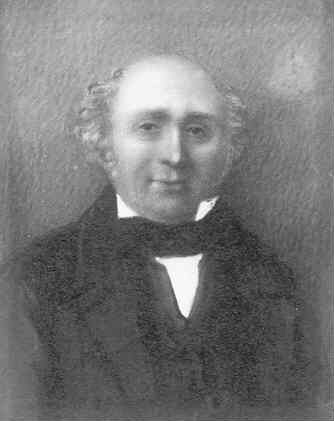
\includegraphics[width=0.42\textwidth]{portrait_benoit_coste.jpg}\par
    \vspace{0.4cm}
    {\small \textit{Benoît Coste (1781--1845)}\par}
    \vfill
\end{titlepage}

\newpage
\pagestyle{plain}
\tableofcontents
\newpage

\pagestyle{fancy}

\part*{Première Époque (1781--1801)}
\addcontentsline{toc}{part}{Première Époque (1781--1801)}

% ===================================================
% CHAPITRE 1
% ===================================================
\chapter{Premières années et Jeunesse (1781--1800)}

Je suis né à Lyon, le sept avril 1781. Mon père était marchand de soie ; il possédait une fortune qui, sans être considérable, était honnête. Il était généralement aimé et estimé, et il le méritait, soit par la loyauté de son caractère, soit par l'aménité de ses manières ; de plus, il était doué d'une qualité assez rare : il avait un excellent jugement.

Ma mère, aussi fille d'un marchand de soie, se distinguait par la vivacité de sa foi et l'ardeur de sa charité. On peut dire que, toute sa vie, cette charité qui remplissait son cœur a dirigé toutes ses actions. J'avais trois sœurs, toutes mes aînées : Madeleine, Catherine et Adélaïde.

Je fus baptisé le lendemain de ma naissance, et on me donna le nom de Benoît, qui était celui de mon grand-père paternel.

Les premières années de mon enfance ressemblèrent à celles de tous les autres enfants. Je passai à la campagne, comme c'était l'usage alors, les trois premières années de ma vie. Dès que je fus rentré dans la maison paternelle, ma mère commença à jeter dans mon jeune cœur ces semences de foi et de religion qui, grâce au Seigneur, n'ont jamais été étouffées. Cette excellente mère employait la plus grande partie de son temps à l'éducation de mes sœurs et à la mienne.

\section*{Le costume d'enfance}

Je vais vous dépeindre mon costume pour ne point laisser échapper l'occasion de vous parler des modes et des usages anciens, pour que vous puissiez les comparer à ceux d'aujourd'hui.

Lorsque j'étais en toilette, j'avais un juste-au-corps et une culotte de soie brochée fond blanc avec des petites bouquets verts et rouges ; des bas de fil blanc, une collerette ; une écharpe de soie verte en ceinture avec un gros nœud à gauche, dont les bouts ornés de franges me tombaient presque jusqu'aux talons ; à la jarretière de la culotte et aux souliers, des boucles de diamants (faux bien entendus,) ou de similor, autre fausseté car ce n'est que du cuivre doré. Les cheveux ondoyants sur les épaules et point de chapeau : ma mère voulait m'accoutumer à ne pas craindre les intempéries de la saison, et cela avait encore un autre avantage, c'est que cela m'évitait de les perdre. Vous jugez que, dans cet accoutrement, je devais être assez joli garçon et, lorsque, sur le quai St Clair, précédant fièrement en guise de Suisse ma petite sœur Adélaïde, une petite badine à la main pour remplacer la hallebarde, je criais : "Place à ma sœur !" on pouvait facilement m'apprécier pour ce que j'étais : un petit étourdi.

Il y avait cependant temps pour tout. Cela ne m'empêchait pas d'apprendre à lire, ensuite mon catéchisme, et, de plus, la grammaire française. Lorsque je fus parvenu à l'âge de six ans, grâce aux soins de ma bonne mère, j'étais déjà assez avancé dans cette petite science de mon âge pour que l'on se décidât à me faire passer mes journées dans un externat, afin de commencer à apprendre à déclamer et à conjuguer le latin.

\section*{Premières études}

Me voilà donc passant mes journées à un 4\up{e} étage de la rue du Théâtre chez un Monsieur Asme...... (...)

D'après l'aveu que je vous ai fait de mon ignorance sur la personne de monsieur Asme, vous avez bien dû pressentir que la science que j'ai pu acquérir auprès de lui n'est guère demeurée gravée dans ma mémoire ; cependant, je trouve dans mes souvenirs que c'est chez lui que, pour la première fois de ma vie, j'ai mis le nez dans \textit{Télémaque}. N'oublions pas d'ajouter un autre souvenir de ce premier pas que j'ai fait dans la carrière de la vie, c'est celui de ces papiers de biscuits que nous achetions à deux liards la feuille pour avoir le plaisir de lécher, de savourer la douce empreinte qui témoignait du passage de ces pâtes exquises.

Parvenu à l'âge de sept ans, beaucoup plus, à ce que je crois du moins, grâce aux soins de ma bonne mère qu'à ce que je pouvais avoir appris chez monsieur Asme, je savais parfaitement mon catéchisme et ma grammaire française, et je commençais à décliner et à conjuguer le latin. La santé de ma mère était altérée et mes grands parents craignirent que les peines qu'elle prenait pour Monsieur son fils ne lui fussent nuisibles. D'après leur avis, on me fit entrer au Grand Collège de Lyon, tenu alors par les Pères de l'Oratoire.

\section*{Le Collège et la Révolution}

Je ne fus point du tout fâché de cette décision : d'abord, c'était un changement et tout changement plaît à cet âge, mais ce qui me ravissait par-dessus tout, c'était la perspective de porter l'uniforme. Je vous ferai donc le portrait d'un écolier du collège ; comme cet uniforme a été plusieurs fois modifié, je m'arrête au premier dont on m'a revêtu.

Nous portions un ample habit bleu, fait à la française, c'est-à-dire à un seul rang de boutons ; il avait de grands pans qui retombaient jusqu'au milieu de la jambe. Il était doublé de serge rouge ; la culotte et la veste étaient en drap rouge. Tous les boutons en cuivre étaient rayés en cercle ; des bas de laine gris, des boucles de cuivre aux souliers et à la jarretière de la culotte ; un tout petit col venait me prendre à la gorge. Ma tignasse bien pommadée et bien poudrée était collée contre ma tête et les cheveux de derrière, enfermés dans un ruban, formaient une queue bien serrée contre la nuque, c'était ce que l'on appelait une queue à la prussienne ; un petit chapeau à trois cornes couronnait tous ces élégants édifices.

Dans une maison qui réunissait 200 élèves, il était impossible de me suivre comme un enfant de cet âge aurait eu besoin de l'être ; d'ailleurs, le système de nos maîtres n'était pas de gagner les cœurs des enfants qui leur étaient confiés et de trouver par là le moyen de les conduire. Ils avaient à leur usage un luxe de sévérité et de punitions, à l'aide duquel ils faisaient régner l'ordre à l'extérieur, ce qui leur suffisait, ils ne demandaient rien de plus.

À cette époque, la révolution qui commençait excitait partout une effervescence dont les maisons d'éducation n'étaient point exemptes. Il en résulta que le séjour de trois ans que je fis au collège me fut extrêmement nuisible. Et j'ajoute que la paresse était alors mon défaut mignon. Personne ne m'aidait à le combattre. Heureusement, la Providence a veillé sur moi d'une manière toute paternelle et elle m'a préservé de grands dangers : c'est dire que je Lui dois plus qu'à la surveillance de nos maîtres, qui était à peu près nulle ; grâce à elle, ma foi ni mes mœurs n'ont reçu aucune atteinte.

S'apercevant du peu de fruit que je recevais de cette éducation, mes parents se décidèrent, dans le courant de l'année 1791, à me rappeler dans la maison paternelle. Cela devenait d'autant plus nécessaire que, la plupart de nos maîtres ayant adhéré au schisme constitutionnel et reconnu l'évêque intrus, me laisser dans cette maison eût été confier mon éducation à des schismatiques.

Comme nous aurons souvent l'occasion de parler dans cet ouvrage de l'église constitutionnelle, il est bon de vous donner immédiatement une explication à ce sujet. On a donné le nom de constitution civile du clergé à une loi par laquelle l'assemblée dite nationale avait, dans les premières années de la révolution, réglé, sans le consentement du Chef de l'Église, toute la hiérarchie de l'église de France, qu'elle rendait à peu près indépendante du St Siège. Le Pape et tous les évêques de France, moins quatre, avaient condamné cette entreprise impie et audacieuse. S'endurcissant de plus en plus et persévérant dans la voie du schisme, le gouvernement exigeait de tous les prêtres un serment d'adhésion à cette constitution civile du clergé ; on a appelé "prêtre constitutionnel" ou assermenté celui qui a eu la faiblesse de se soumettre à cette exigence ; celui qui, au contraire, demeurait fidèle à l'unité catholique méritait le nom de "prêtre réfractaire" ou insermenté. Enfin, les évêques et les curés qui, sous la protection des autorités civiles, ont pris la place des pasteurs légitimes chassés à cause de leur résistance aux injonctions des schismatiques ont pris le nom d'évêques ou de curés intrus.

Je suis donc rentré chez mes parents en 1791. Ils me confièrent à un jeune ecclésiastique plein de vertu et de talents qui s'appelait monsieur Satin ; c'était un vicaire de monsieur Linsolas que vous avez connu ; il était vicaire de Vaugneray et avait refusé le serment, ce qui faisait qu'on l'avait chassé de son poste.

Malgré les conseils d'un homme aussi supérieur, j'avais gardé les habitudes de paresse que j'avais contractées au Collège. On crut triompher de ce misérable défaut par des voies de rigueur, vieille marotte qui était encore un peu en usage, mais on se trompa, on ne parvint qu'à m'aigrir le caractère et à m'exaspérer. Cette fâcheuse disposition s'empara si fort de mon âme qu'un jour je pris la résolution insensée de fuir la maison paternelle. Je m'évadai donc, sans chapeau et avec, pour tout bien, une pièce de trente sols dans ma poche. Je pris la route de Montluel, forgeant dans ma petite cervelle mille projets divers, comme d'aller m'offrir en qualité de tambour aux émigrés rassemblés sur les bords du Rhin, ou bien de me placer auprès d'enfants plus jeunes que moi pour leur communiquer ma science. Heureusement, la Providence dirigea mes pas et me fit entrer pour demander asile dans une maison bien chrétienne. La maîtresse de la maison m'admit le soir à la prière commune et me chargea même de faire la lecture ; en me remettant le livre, elle eut soin de choisir l'histoire de l'enfant prodigue. Je me suis bien douté que j'étais deviné mais n'en fis pas semblant. Le lendemain, un domestique de mes parents, envoyé pour me découvrir, me ramena à la maison.

Le système adopté ne fut pas changé et, persuadé que mes parents ne m'aimaient pas, -- alors qu'ils me chérissaient, -- je continuais de vivre dans un état tout à fait violent. Je ne travaillais plus que comme un esclave, dans la crainte du châtiment. Cette pénible situation dura environ un an.

% ===================================================
% CHAPITRE 2
% ===================================================
\chapter{Souvenirs du Siège de Lyon et de ses suites (1793)}

La persécution, dont les rigueurs s'aggravaient de jour en jour, força vers ce temps-là monsieur Satin à se séparer de nous et à quitter la France. Je le vis partir avec beaucoup de peine car, malgré que nous fussions loin d'être toujours d'accord, je l'aimais bien sincèrement et, de son côté, il avait beaucoup d'amitié pour son élève. Cette année n'avait pourtant pas été perdue pour moi et les soins assidus de mon professeur m'avaient fait faire dans l'étude du latin des progrès assez sensibles. Il avait su aussi développer en moi les semences de foi que les instructions de ma mère avaient placées dans mon cœur.

\begin{quote}
\textit{(Après le départ de M. Satin, Benoît Coste est confié à un Sulpicien, M. Molin, qui avait été, lui aussi, chassé du séminaire. Il ne restait alors que de rares églises ouvertes au culte et Benoît Coste allait tous les jours servir la messe dans la chapelle des Joséphistes.)}
\end{quote}

Au 29 janvier 1792, les Dames de la Visitation de Ste Marie de Bellecour étaient encore dans leur couvent, dans lequel était mort St François de Sales et où l'on conservait le cœur du saint. Cette précieuse relique était exposée à la vénération des fidèles pendant trois jours consécutifs, à l'époque de la fête du saint, et les prêtres s'empressaient de venir dire la messe en sa présence.

Monsieur Satin partagea la dévotion commune ; et il y fut, et je lui servis la messe. Or, mes enfants, il faut que vous sachiez que ces dames étaient en usage d'offrir à déjeuner pendant ces trois jours à tous les prêtres qui venaient célébrer dans leur église. Mon précepteur avait la plus grande envie d'éviter ce déjeuner mais moi, qui savais que le clerc devait passer par dessus le marché, j'étais animé d'un sentiment tout contraire. Malheureusement, ce n'était pas moi qui faisais la loi. Pour sortir de la maison, il fallait, en quittant la sacristie, descendre un escalier alors que, pour aller trouver le bienheureux déjeuner, il le fallait monter. Voilà qu'après avoir terminé son action de grâces, mon maître me dit tout bas :
-- Allons-nous en vite, avant qu'on ne nous voie !

En même temps, il ouvre la porte et commence à descendre. Je n'étais pas content mais n'ose sais rien dire. Comme St Pierre, je suivais de loin, le plus lentement que je pouvais. Tout à coup, ô bonheur ! j'entends la voix de la tourière :
-- Monsieur, monsieur !
-- Monsieur, lui dis-je, on vous appelle.

Il entendait aussi bien que moi mais ne s'en sauvait que plus vite, et cela était loin de faire mon compte. Heureusement, la tourière, voyant qu'on ne lui répondait pas et venant peut-être aussi au secours d'un désir que trahissait ma voix enfantine, précipite ses pas, rejoint mon homme, parvient à le ramener et le fait entrer tout penaud dans la salle du festin. Quelle bonne fortune pour un écolier de onze ans !

Peu d'années après, ce bon monsieur Satin partit pour le Canada avec monsieur Molin et quelques autres membres de la compagnie des Sulpiciens fixés au séminaire de Montréal. Il y est mort en 1836.

Après le départ de monsieur Satin et avant qu'ils eussent pu prendre une détermination définitive, mes parents jugèrent à propos, dans l'espoir de vaincre ma paresse, de me soumettre à une nouvelle épreuve. Ils m'annoncèrent que, puisque je ne voulais pas étudier, ils allaient me mettre chez un ouvrier en soie, pour apprendre un état mécanique et, effectivement, je fus envoyé en qualité d'apprenti chez un vénérable et saint patriarche qu'on appelait monsieur Durol. Il faisait marcher, avec le secours de sa femme et de ses trois filles, un atelier considérable d'étoffes de soie. Je ne fus pas là deux jours qu'il me fut facile d'apprendre qu'on ne m'y avait pas placé pour apprendre sérieusement l'état. On m'installa à la vérité à un rouet à cosmette mais je n'y travaillais qu'autant que cela me convenait. Tout le monde me gâtait, on s'amusait de mon petit babil et une partie de la journée était employée à feuilleter la bibliothèque très bien montée du fils de la maison, jeune homme de vingt ans qui étudiait pour être prêtre. Les deux mois de séjour que je fis dans cette maison furent donc complètement perdus par rapport à ma disposition de paresse. Les exemples d'édification que j'ai eus sous les yeux n'ont cependant pu qu'être avantageux pour le bien de mon âme.

Vers le commencement de 1793, on imagina un nouveau moyen de vaincre mon dégoût du travail. On décida de me laisser sans rien faire et, en même temps, on défendit à mes sœurs de s'amuser avec moi. Je passais donc ainsi de longues journées sans qu'il me fût seulement permis de toucher un livre. Je succombais à l'ennui, aussi je crois que ce moyen aurait réussi si, après m'avoir tenu pendant quelque temps à ce régime, on eût essayé de me permettre de reprendre le travail. Pourtant, d'autres épreuves m'attendaient.

Un matin, sans qu'aucune faute nouvelle de ma part eût donné un motif plausible à cette scène, mon père entre dans ma chambre, paraissant fort en colère car je n'étais pas encore levé. Il me déclare qu'il ne veut plus d'un vaurien ni d'un paresseux dans sa maison et que, s'il me retrouve lorsqu'il rentrera pour dîner, il me cassera bras et jambes. Sans ajouter un mot, il disparaît.

Cette fureur apparente, si peu dans le caractère de mon père, me remplit de consternation. Ahuri et tremblant, je me lève en gémissant. Je suis à peine habillé que je vois entrer dans ma chambre ma sœur aînée. Elle vient me demander quel parti je veux prendre.
-- Eh ! Que veux-tu que je fasse ? lui répondis-je en sanglotant. Mon père me chasse, il faut bien que je m'en aille !

Ma mère survient, elle me conseille de me réfugier chez une grand tante qui était pleine de bonté pour moi, elle m'ajoute que, par grâce, elle veut bien m'accompagner. On me conduit à l'armoire où sont mes hardes, on me fait faire un petit paquet. Je le place sous mon bras et, donnant la main à ma mère, je passe en pleurant le seuil de l'appartement. Chez ma tante, nouvelle scène, on défend solennellement à mes cousins de s'amuser avec moi parce que je suis un mauvais sujet qui ne peut que leur donner de mauvais conseils et de mauvais exemples.

Ma mère me quitte, ma tante se retire, on me laisse seul, livré à mes réflexions, qui étaient fort tristes. J'étais accablé de douleur, une multitude de pensées s'offraient tour à tour à mon imagination de douze ans. Ma situation était affreuse, je me voyais abandonné par mes parents, sans pouvoir trouver aucun moyen de parvenir en grâce avec eux. Une heure s'écoula ainsi. Ma mère revient :
-- Monsieur, me dit-elle, j'ai été assez heureuse pour trouver un pension où l'on veut bien vous recevoir, je vais vous y conduire.

Ces paroles firent sur moi un effet magique. En un clin d'œil, tous mes chagrins furent dissipés : la colère de mon père, le froid glacé de ma mère, la sévérité apparente de ma tante, tout cela ne fut plus à mes yeux que le résultat d'un plan combiné pour opérer sur mon esprit une impression plus vive, car enfin, me disais-je \textit{in petto}, une pension ne se choisit pas et ne s'arrête pas en une heure de temps ! il est évident que tout cela était préparé et calculé d'avance.

Je suivis donc ma mère, toujours portant mon petit paquet, beaucoup moins pesant alors. C'est ainsi que nous arrivons à la pension destinée à me recevoir. Elle était tenue par un certain monsieur Reydellet. Ma mère m'y laisse et me voilà tout joyeux, lancé au milieu de mes nouveaux camarades. Il était d'usage dans ce pensionnat que l'entrée d'un nouvel écolier fût célébrée par une demi-journée de vacance. Je trouvai ce règlement admirable et cette journée si tristement commencée se termina donc dans les jeux. Comme c'était la coutume, mes nouveaux compagnons m'éprouvèrent par quelques petites farces dont je fus le premier à rire, ce qui me valut l'amitié de mes camarades.

Le régime de cette pension me convenait à merveille car il y avait beaucoup de récréations et peu de travail. Malgré ma paresse et mon étourderie, je fus immédiatement rangé parmi les enfants dont on était content. M. de Viller, prêtre zélé qui, au péril de sa vie, exerçait alors le saint ministère dans notre ville était l'aumônier de la pension. C'est lui qui l'avait indiquée à mes parents.

Ce prêtre me prit en particulier quelques jours après mon entrée, m'engageant à écrire à mon père, qu'il me peignit comme fort en colère, pour lui demander pardon et le supplier de me rendre ses bonnes grâces. Persuadé que le passé n'était qu'une comédie, je ne croyais pas du tout à la grande colère de mon père mais je promis cependant d'écrire et, dès le lendemain, remis à M. de Viller une lettre où, dans les termes les plus soumis, j'implorais mon pardon.

Quinze jours se passent sans réponse. À ce moment, une circonstance fortuite vint me tirer de peine. J'étais en promenade avec la pension quand, passant dans une des rues de la ville, nous rencontrons un cortège dont mon père faisait partie. Il m'aperçoit et son cœur paternel est ému : oubliant le rôle qu'on lui faisait jouer mais ne pouvant venir à moi, il me regarde avec des yeux emplis de bonté. Ce sourire d'amitié porta la consolation et le bonheur jusqu'au fond de mon âme.

Le soir même, M. de Viller vient me dire que mon père est toujours fâché contre moi et qu'une seule lettre ne suffit pas, qu'il faut que j'écrive de nouveau.
-- Non, Monsieur, non ! répondis-je avec vivacité, non Monsieur, mon père n'est plus fâché contre moi !
-- Et comment le savez-vous, me dit-il sèchement ?
-- Je l'ai rencontré ce matin : quand on est fâché contre quelqu'un, on ne lui sourit pas comme il m'a souri !

Je n'en écrivis pas moins une seconde lettre et, pour toute réponse, mon bon père vient me voir, m'embrassa de bon cœur et tout fut terminé.

Il était de règle dans la pension Reydellet que, chaque année, il y avait un jour de congé particulier et une grande promenade pour les plus sages de la pension. La condition en était la remise de quarante exemptions. Ces exemptions s'obtenaient à titre de récompense et avaient cours pour épargner les punitions. La promenade était annoncée le lendemain et, pour y participer, il fallait quarante exemptions ; il fallait déposer la veille, c'est-à-dire le jour même, les titres voulus or, si j'avais beaucoup d'exemptions, je n'en avais pas le compte. J'ai beau tourner et retourner mon portefeuille, compter et recompter, je ne puis en trouver plus de trente-cinq. Que faire ? Je veux pourtant être de la promenade, qui ne doit revenir que dans un an. Tout bien pesé et considéré, je m'arrête à ce qui me paraît avoir plus de chances de succès, je vais confier ma peine à l'un de nos maîtres, Monsieur Cottin, et lui dis timidement :
-- Monsieur, je n'ai que trente-cinq exemptions. Vous savez que j'en gagne assez souvent ; vous pourriez me tirer d'embarras : si vous vouliez seulement m'avancer une exemption de cinq, cela me ferait mon compte et, à la première occasion, je vous la rendrai fidèlement.

Ma demande fit sourire le digne prêtre, qui y satisfit sans hésiter et me permit d'être de la bienheureuse promenade. Il me souvient encore que nous fûmes aux Brotteaux et que nous pêchâmes des grenouilles dans un petit bras du Rhône qui passait près de la Tête d'Or.

Quelques jours après, j'obtins mes cinq exemptions que je rapportai fidèlement à Monsieur Cottin, qui eut la générosité de ne pas vouloir les reprendre.

\section*{Coup d'œil sur la Révolution}

Alors que je me livrais aux joies et aux plaisirs de mon âge, une cruelle révolution promenait déjà sa faux meurtrière sur notre malheureuse ville. Avant de rappeler ces tristes souvenirs, jetons un coup d'œil en arrière pour considérer les causes qui ont attiré tant de maux sur notre infortunée patrie.

Il y a plus de trois siècles que le démon de l'orgueil a proclamé par la bouche de ses suppôts, -- Luther, Calvin et consorts, -- l'indépendance de la pensée en matière de religion. Voulant encore étendre ces maximes de licence, le même esprit de mensonge s'est servi de ceux qui, au dernier siècle, se sont eux-mêmes honorés du nom de philosophes. Ces nouveaux précepteurs du genre humain ont voulu qu'à l'avenir, pour peser les vérités de la foi, le poids du sanctuaire fût remplacé par celui de leur intelligence. Ils ont livré la parole immuable sortie de la bouche même du Très-Haut à tout l'arbitraire des systèmes que leurs imaginations déréglées ont été capables d'inventer.

Quelques-uns d'entre eux ont daigné faire la grâce à Dieu de l'admettre dans le symbole de leur croyance, à la condition, toutefois, que ce serait un Dieu commode qui se bornerait à régner dans le ciel sans se mêler en aucune manière des affaires de ce monde, que surtout il cesserait de les effrayer avec ses peines éternelles de l'enfer, dont ils ne veulent absolument pas car ils les redoutent trop pour y croire. D'autres, plus hardis, n'ont pas voulu reconnaître d'autre dieu que la matière, et certains, poussant à la dernière extrémité les conséquences logiques de leurs principes, ont fini par rejeter entièrement ces notions du juste et de l'injuste que Dieu, par la loi naturelle, a gravées dans le cœur de tous les hommes.

Le même esprit de licence qui portait ces novateurs à secouer le joug de la religion devait aussi les amener à chercher les moyens de se débarrasser de l'autorité des rois. Un grand complot fut donc formé pour détrôner en même temps, si cela eût été au pouvoir de ces hardis conspirateurs, et le Dieu qui règne dans le ciel, et ceux qui le représentent sur la terre.

Considérons cependant comment la Providence, dans Sa sagesse, permet que le châtiment si justamente mérité par l'orgueil insensé de l'impie se rencontre précisément dans le succès de ses projets liberticides. Un roi philosophe l'avait dit : "Si je voulais punir une province, je la donnerais à gouverner aux philosophes !" Pour punir la France qui a applaudi et exalté ce Voltaire, chef d'une philosophie anti-chrétienne, et ses nombreux complices, Dieu, dans sa colère, va la livrer au gouvernement des disciples de cette école d'impureté. Nous pourrons juger de l'arbre à ses fruits amers.

Ces artisans de ruine marchent au but qu'ils se sont proposé, déjà ils ont renversé l'ordre des Jésuites : il fallait bien commencer par détruire ce boulevard redoutable ! Déjà, ils ont travaillé et n'ont que trop réussi à corrompre les mœurs, car ils n'ignorent pas que le désordre de la conduite amène le désordre dans les idées et que l'impureté, presque toujours, est fille du libertinage.

Tout fait alors pressentir une imminente catastrophe. Les ministres du Dieu vivant, le cœur oppressé de douleur, y président du haut de la chaire de vérité et, dans les transports d'une joie satanique, les suppôts de l'enfer l'annoncent au milieu de leurs orgies.

Un seul obstacle pourrait retenir les efforts des méchants, mais combien il sera facile à renverser ! Un digne fils de St Louis porte la couronne de France ; c'est un prince solidement vertueux, également pénétré de ses devoirs envers son Dieu et de ses devoirs envers son peuple, mais son âme est trop belle pour le malheureux temps où il est appelé à régner. Si son trône est encore debout, il ne ressemble que trop aux antiques débris qu'on croirait sains et entiers au milieu de ces cités ensevelies sous la lave d'un volcan : un souffle suffira pour le réduire en poudre.

Déjà, l'agitation commence. Les États Généraux sont convoqués. Le premier acte de cette assemblée soi-disant nationale est un acte de révolte, qui consacre le principe de l'insurrection. Bientôt on attaque la religion par le schisme, en attendant de faire disparaître cette ombre vaine qu'on en conserve un instant encore. On décrète la liberté pour tous, mais cette liberté n'existe que pour le mal, elle est nulle pour le bien. Le Roi est moins libre que personne, il est livré aux attaques des factieux, en butte à leurs outrages. Enfin, le 10 août 1792, on a achevé de détruire ce qui semble encore rester de l'autorité royale, le trône est renversé, l'héritier d'une dynastie de huit siècles est jeté dans les fers.

Quelques jours après, le 2 septembre, d'infâmes scélérats croient anéantir la religion en massacrant des évêques et des prêtres prisonniers et sans défense, mais ils ne réussissent qu'à faire des martyrs.

La révolution ne recule devant aucun crime : une assemblée de factieux ose juger son souverain. Louis XVI, devant ses juges iniques, parle avec la majesté d'un Roi ; dans son immortel testament, il tient le langage d'un saint et, le 21 janvier, victime expiatoire des crimes de son peuple, il meurt avec le courage d'un martyr.

Ceux qui n'ont pas craint de verser le sang de leur roi ne s'arrêtent pas là et le règne de l'échafaud, si justement nommé le règne de la terreur, commence et se personnifie dans le misérable horriblement célèbre sous le nom de Maximilien Robespierre.

Ces scènes d'horreur se passaient à Paris, mais elles trouvaient dans les provinces, et surtout à Lyon, une affreuse imitation : toutes les phases de la révolution s'y reproduisaient tour à tour. Ainsi, en septembre 1792, des prêtres et des officiers furent massacrés à Lyon ; à Paris, on ameutait le faubourg St Antoine et le faubourg St Marceau, à Lyon, c'était les quartiers St Georges et de la Grande-Côte. À Paris, Robespierre et Marat étaient les chefs de ces bandits qu'on a appelés Jacobins, à Lyon, c'était Chalier.

Ce scélérat, après la mort du Roi, forma le projet d'assassiner en un seul jour un grand nombre des principaux citoyens de la ville. Cette tentative fut déjouée mais Chalier, soutenu et encouragé par ses amis de Paris, ne renonça pas à saisir la victoire. La ville était dans une extrême agitation, l'administration départementale avait embrassé le parti des honnêtes gens mais la municipalité, -- au contraire soumise à l'influence de Chalier, -- favorisait les fauteurs de désordre. On avait lieu de craindre les massacres et le pillage.

Le 29 mai 1793, dans la matinée, un bataillon de la Garde Nationale se présente devant l'Hôtel de Ville, où siégeait la municipalité jacobine, pour lui adresser des plaintes sur quelques nouvelles mesures de tyrannie. Une décharge d'artillerie est la seule réponse qu'il reçoit. La vue des blessés et des mourants met l'exaspération à son comble, c'est une étincelle électrique qui porte la plus violente commotion dans tous les quartiers de la ville. Les citoyens courent aux armes, ils se réunissent place Bellecour, dans l'intention d'attaquer à l'Hôtel de Ville cette municipalité anarchique.

Les hommes en armes se mettent en marche sur trois colonnes, par le quai du Rhône, par les rues de l'intérieur de la ville et par le quai de la Saône. Les deux premières colonnes, accueillies par des décharges de mitraille, reculent et sont dispersées ; la troisième, plus heureuse, parvient à la boucherie des Terreaux où elle se cantonne. Là, elle se recrute encore des débris des deux autres. Les avenues de l'Hôtel de Ville sont gardées par un régiment de troupes de ligne et par ceux, heureusement en petit nombre, des Gardes Nationaux qui font cause commune avec les Jacobins.

Pendant le reste de la journée, on continue à échanger quelques coups de canon ; la nuit semble apporter une espèce de suspension aux hostilités. Les sommités jacobines réunies à l'Hôtel de Ville, se croyant sûres de la victoire, la célèbrent d'avance par un repas somptueux et par d'abondantes libations. Pour la plupart, ils sont bientôt réduits à un état complet d'ivresse. Cependant, les Lyonnais tenaient toujours leur poste de la boucherie et ne s'endormaient pas.

Vers 5 heures du matin, leurs canonniers chargent leurs pièces à boules et, les pointant contre la grande porte de l'Hôtel de Ville, les font voler en éclats. La colonne s'ébranle alors ; son commandant, un simple charcutier du nom de Gingesme, marche en tête, à cheval, la bride aux dents et un pistolet à chaque main. C'est ainsi qu'il aborde hardiment le perron de l'Hôtel de Ville ; en un clin d'œil, il en a franchi les degrés et la colonne victorieuse s'empare facilement des autorités révolutionnaires dont le vin avait troublé la raison et rendu les pas chancelants. Ceux qui s'étaient voués à leur défense fuient ou se rallient aux Lyonnais. Tous ces hommes qui avaient conspiré la perte de la ville et le massacre de ses principaux citoyens sont conduits en prison.

Telle fut l'issue de cette journée qui avait occasionné de cruelles inquiétudes à tous les honnêtes gens. Nous nous étions couchés le 29 au soir, dans notre pension, avec la douleur dans l'âme comme tout le monde, croyant alors au triomphe de ceux que l'on appelait, dans le langage du temps, les sans-culottes ou les clubistes. Quelle fut notre surprise et notre joie lorsque, le 30 au matin, nous fûmes réveillés par les chants de victoire. Nous n'eûmes plus qu'à rendre grâce au Seigneur.

Cet événement valut à Lyon quelques mois de tranquillité. Malheureusement, la révolution vaincue dans notre ville avait triomphé à Paris. La journée du 31 mai avait plus que jamais affermi le pouvoir des Jacobins. Ces hommes de sang, furieux de l'échec essuyé à Lyon, résolurent d'employer tous les moyens à leur portée pour nous faire courber la tête sous leur joug de fer et annoncent donc qu'ils vont avoir recours à la force.

De son côté, à Lyon, on se prépare à la défense. Les habitants sont pourtant loin d'être complètement unis dans une même pensée et dans un même sentiment ; les autorités surtout, c'est-à-dire l'administration du département et la municipalité provisoire formée des présidents des différentes sections ou quartiers de la ville, qui ne partageait point le désir d'un grand nombre de nos concitoyens de profiter de la victoire pour revenir à l'ancienne monarchie sous le gouvernement de laquelle nos pères avaient trouvé le bonheur. Ces magistrats républicains modérés se bornaient à résister à un gouvernement de sang, mais ils voulaient eux aussi la république et c'est sous le drapeau tricolore, ce drapeau de la révolte, qu'ils se disposaient à combattre l'anarchie.

Avant l'investissement de notre ville, on instruisit le procès des chefs des Jacobins. Une procédure régulière fit connaître au public les crimes affreux dont ils s'étaient rendus coupables et deux d'entre eux, -- Chalier, leur chef, et un nommé Riard, -- furent condamnés à perdre la tête sur l'échafaud. Remarquons au passage comment il plaît au Très-Haut de montrer quelquefois avec évidence les dispositions de sa justice : Dans sa rage sanguinaire, Chalier avait fait venir à ses frais, de Paris, cette machine de mort inventée par les Jacobins pour procéder avec plus de rapidité à leurs barbares exécutions et qu'on a appelée la guillotine ; il avait formé le projet de la placer sur le pont Morand et de s'en servir pour se débarrasser de tous les négociants qui lui faisaient ombrage ; ce fatal instrument n'avait pas encore servi et c'est pour abattre sa tête coupable qu'un bourreau maladroit en a fait l'essai ; comme si le ciel eût voulu rendre plus cruel le supplice de ce scélérat, il fallut y revenir à cinq fois pour terminer et ses souffrances et sa vie.

Cependant, les troupes révolutionnaires s'étaient mises en marche. La jeunesse de la ville se dispose à les bien recevoir. Pour faciliter la défense par une exacte discipline, on invite les hommes de bonne volonté et dans la force de l'âge à quitter le toit paternel pour se résigner à la vie du soldat. Six mille hommes environ répondent à cet appel ; ils vont habiter les casernes et prennent le nom de casernés. Pantalon et veste de nankin, point de gilet ni de cravate, voilà tout l'uniforme de ces braves.

Monsieur de Précy, gentilhomme de Bourgogne, ancien militaire, est appelé à Lyon et se charge de la défense de la ville dont il prend le commandement militaire. Si tous les pouvoirs eussent été remis entre les mains de ce général en chef, lui et ses braves casernés auraient promptement arboré le drapeau blanc et proclamé comme notre légitime souverain, sous le nom de Louis XVII, le fils infortuné de notre Roi Martyr. Cette énergique résolution eût peut-être assuré le succès de la plus juste et de la plus noble des causes, mais il avait été arrêté par les décrets éternels que la justice de Dieu devait s'appesantir sur nous. On ne fit donc rien de ce qu'on aurait dû faire, car nous étions pour lors livrés à la puissance des ténèbres.

Enfin, il n'est plus possible d'en douter, nous allons être attaqués. Qu'ils furent tristes pour nous, pauvres écoliers, les trois jours qui précédèrent le siège ! Nous avions alors été transférés des Grands Capucins dans une maison occupée avant la révolution par une Providence et maintenant occupée par les dames Carmélites. Cette maison est située sur la colline de Fourvière, de manière à dominer la ville, et nous y parvenaient les sons lugubres et accélérés du tocsin qui, de tous les clochers, annonçaient les malheurs qui allaient fondre sur la cité. Puis ce bruit effrayant fit place au bruit plus terrible encore de la canonnade, de la fusillade et du bombardement.

Nos casernés volent aux avant-postes et y font des prodiges de valeur. Les avantages marqués qu'ils remportent les premiers jours augmentent leur courage et leur ardeur. Les habitants du Forez, dans une déchirante et douce confraternité, rivalisèrent de zèle avec ceux de Lyon. On pouvait encore communiquer avec St Etienne et avec Montbrison. Au bout de quelques jours, cette ressource nous fut enlevée et nous fûmes environnés de toutes parts. Des représentants de cette assemblée de brigands qu'on a appelée Convention avaient été envoyés pour réduire la ville par le fer et par le feu ; ils imaginent de porter la discorde et la désunion parmi les habitants en engageant ceux-ci à se séparer des autorités et à faire leur soumission particulière. On rédige à l'instant une réponse, qui est revêtue, au milieu même de la place des Terreaux, de vingt mille signatures ; cette réponse annonce la volonté de toute la population de résister à l'oppression et de rester sur la brèche pour se défendre.

Et pendant ce temps de si triste mémoire, dans notre pension, nous gémissions des maux de la patrie ; nous suivions le mouvement des bombes qui tombaient sur la cité et, parfois, arrivaient jusqu'à nous. Si on nous eût laissé faire, nous, jeunes écoliers, nous eussions été tout à fait disposés à aller aux avant-postes. En fait, nous avons pris notre part des privations que nous imposait l'état de siège car la famine commençait à se faire sentir. Monsieur Reydellet avait pris ses précautions, il avait fait d'amples provisions de farine mais le siège se prolongeait et on commençait à craindre que ces provisions ne fussent pas suffisantes. Il prit donc le parti de nous mettre à la ration et, chaque matin, nous recevions tous une livre de pain ; nous avions pleine liberté de nous servir de notre portion à volonté. Les élèves, par l'usage qu'ils faisaient de leur pain, montraient leur caractère : Quelques-uns mangeaient tout à déjeuner, sauf à jeûner le reste du jour ; de petits avares, crainte de manquer, le laissaient durcir, sans oser y toucher, au point qu'il devenait immangeable ; d'autres, seulement économes, en conservaient pour le déjeuner du lendemain. Un certain nombre le divisait convenablement entre les quatre repas de la journée ; enfin, il s'en trouvait quelques-uns qui rognaient un morceau de leur portion pour venir au secours de leurs camarades trop affamés. Quant à moi, je l'avoue, je partageais mon pain entre mes quatre repas et, quand il y en avait de reste, -- mais cela n'arrivait pas tous les jours, -- j'en faisais profiter un ami.

Les assiégeants gagnaient toujours du terrain et nous resserraient de plus en plus, les pauvres casernés étaient sur les dents. Il n'y avait de repos pour eux que de passer d'un poste périlleux à un autre moins exposé. Le 29 septembre, les assiégés et leur général, Précy, se couvrirent de gloire. La ville fut attaquée de cinq côtés différents ; après avoir repoussé l'ennemi sur un point, Précy s'empressait de voler sur un autre, et sa présence suffisait à assurer la victoire. Elle fut complète en ce jour mais, hélas ! c'était la lueur d'une lampe qui s'éteignait : cent mille hommes environnaient la ville et la mort avait fait de grands vides parmi les héroïques défenseurs. La famine se faisait sentir et l'on avait perdu espoir d'être secouru. Après deux mois de siège, l'issue ne pouvait faire de doute.

Précy voulut essayer du moins de sauver avec lui ce qui restait des intrépides défenseurs de la cité. On sort par la porte de Vaise, espérant gagner la Bourgogne et, à travers la Franche-Comté, se réfugier en Suisse. Cette sortie échoua complètement. Avec un détachement de cinquante hommes, Monsieur de Précy parvint dans les bois d'Alis, où il se sépara de ses fidèles compagnons qui cherchèrent, chacun comme il put, à se dérober aux perquisitions des terroristes. Quant aux Lyonnais qui avaient fait partie de cette sortie désespérée, ils furent tous massacrés par les paysans, ou faits prisonniers, et ramenés à Lyon. Mon oncle Jordan fut du nombre de ceux-ci ; heureusement, grâce à quelques apparences de douceur et d'humanité par lesquelles on chercha dans les premiers jours à rassurer la population, il fut mis en liberté et pu se soustraire à une seconde arrestation dont la suite eût été véritablement la mort.

Les troupes révolutionnaires prirent donc possession de la ville et bientôt Lyon fut comme Paris, comme Nantes et plusieurs autres villes de France, placé sous le niveau sanglant de la Révolution. La guillotine, d'abord dressée sur la place des Terreaux puis transférée à Bellecour, pour être remise aux Terreaux, fut solidement placée sur un échafaud permanent peint en rouge. Les représentants de la Convention, des cannibales, habitaient la rue Ste Catherine ; comme une maison leur masquait la vue si agréable pour eux de la guillotine, ils la font abattre, ce qui leur permet de se délecter en comptant toutes les angoisses qui accompagnaient les derniers moments de leurs victimes.

Quelque promptitude que pût apporter l'instrument de mort à répandre le sang de nos concitoyens, il était encore trop peu expéditif au gré de nos tyrans. Il leur fallut la balle meurtrière qui vint suppléer à la lenteur du fer homicide et le canon, pointé avec une joie féroce contre une troupe nombreuse de victimes, fut charged d'accélérer encore l'effroyable rapidité du carnage. Lorsque quelque malheureux conçoit l'espérance d'échapper à la mort, à la faveur du grand nombre, des bourreaux organisés en grand nombre pour cet odieux service se précipitent sur l'horrible champ de bataille pour achever à coups de sabre la victime épargnée par la mitraille.

Toute marque de deuil, tout signe de pitié, la moindre sympathie à l'égard des malheureux immolés à ce que l'on appelle la vengeance nationale est un crime irrémissible jugé digne de mort.

La rage de ces hommes de sang n'est pas satisfaite par ces torrents de sang innocent, il lui faut encore s'assouvir par la destruction des objets inanimés. Les plus beaux édifices de la cité sont renversés et ils vont jusqu'à changer le nom de l'infortunée ville de Lyon en celui de \textit{Commune Affranchie}.

Pendant cette triste époque, nous avons perdu trois parents, parmi lesquels mon grand-père maternel. Mon grand père paternel était mort en 1793, s'il eût vécu, il n'aurait pas été épargné ; quant à mon père, Dieu, dans sa miséricorde, nous le conserva miraculeusement.

Dès la prise de la ville, ma mère voulut le faire sauver mais mon père n'accepta pas, par égard pour son frère aîné qui a, hélas, payé de sa tête sa fatale sécurité. Mon père, donc, ne fut arrêté qu'au bout de trois semaines ; après deux mois de détention, il fut appelé devant les assassins qu'on nommait le Tribunal révolutionnaire et fut envoyé à la cave de gauche de l'Hôtel de Ville, de laquelle on ne sortait que pour mourir. Parmi les condamnés se trouvaient quelques jeunes gens qui avaient pensé tenter une évasion ; après des efforts inouïs, ils parvinrent à trouver une issue par des corridors souterrains. Mon père fut averted et eut le bonheur d'être du petit nombre de ceux qui parvinrent à s'échapper.

J'étais instruit de sa condamnation, je savais que, le jour même (jour mémorable, c'était le 11 décembre), il devait être exécuté et, comme vous le pensez bien, j'étais abîmé de douleur. C'était le matin, nous étions tous encore couchés dans le dortoir ; mon voisin m'entend sangloter.
-- Mon ami, me dit-il, tu te désoles et tu as tort ; j'ai la conviction intime que ton père se sauvera ; sois sûr qu'il échappera, je t'en réponds !

Hélas, toutes ces assurances ne me tranquillisaient guère et cependant c'était l'heure même où Dieu l'arrachait à la fureur de ses bourreaux.

Pendant ce temps affreux, il n'était guère possible de s'occuper d'études ; maîtres et disciples, nous étions tous préoccupés des scènes horribles que nous avions sous les yeux. La prière était notre occupation principale, encore fallait-il se cacher pour cela : nos Heures nous avaient été enlevées, un livre de prières eût pu occasionner un arrêt de mort ; nous n'avions pour toute la communauté que deux paires d'Heures que nous tenions cachées entre nos tiroirs. Nos récréations se passaient fort tristement, nous n'avions pas le courage de nous amuser. On nous faisait apprendre par cœur les droits de l'homme, dont, entre nous, nous faisions gorges chaudes, mais nous étions cependant tenus d'être en état de les réciter en cas de visite. Pour nous attirer la bienveillance de nos seigneurs et maîtres les citoyens sans-culottes, quelques-uns d'entre nous, et j'étais du nombre, avaient été chargés d'apprendre à lire aux petits galopins du quartier.

Après son évasion, mon père resta trois semaines caché dans la ville. Vers la fin du mois de décembre, à l'aide de faux papiers, il parvint à gagner la Suisse. Craignant qu'on ne mît à mon égard à exécution une mesure dont on avait menacé, d'enlever les enfants des condamnés pour en faire des mousses, ma mère jugea à propos de me faire sortir de pension et me fit entrer sous un faux nom chez un ouvrier en soie nommé Tissot qui nous était un peu parent. Je passais pour son neveu.

Ainsi se sont terminées mes études de latin. Malgré toute ma paresse, ces différentes interruptions et la perte presque totale des derniers mois, j'étais parvenu à être un troisième passable. Je ne suis guère resté que six semaines chez Tissot car ma mère prit la résolution d'aller rejoindre mon père en Suisse avec tous ses enfants. Il y avait alors une entreprise qui, moyennant une somme déterminée, vous fournissait un passeport, applanissait toutes les difficultés sur la route et se chargeait de vous rendre sains et saufs à Genève.

Nous profitâmes donc de cet expédient et partîmes sous un faux nom. Nous avons voyagé à petites journées. Le premier jour, pour ne pas éveiller l'attention des tyrans, nous sortîmes de la ville en trois bandes, et à pied. Nous fûmes ainsi jusqu'à l'Hôtel d'Henri IV, un peu plus loin que la Boucle, où nos effets avaient été déposés d'avance. Nous y trouvâmes notre voiture et fûmes coucher à Meximieux. Le second jour, nous couchâmes à Nantua, le troisième à Collonge et, le quatrième, dans la matinée, nous étions à Genève, d'où nous partîmes le soir même pour nous rendre plus tôt auprès de mon père.

% ===================================================
% CHAPITRE 3
% ===================================================
\chapter{Souvenirs de Constance (1794--1796)}

Nous nous embarquâmes donc sur le lac avec d'autres Lyonnais qui, comme nous, fuyaient la tyrannie révolutionnaire. Il y avait entre autres le fameux Gingesme, le héros du 29 mai. Il n'avait pour lors qu'une seule jambe, l'autre ayant été emportée pendant le siège par un boulet de canon. À peine eûmes-nous quitté le port que, d'un mouvement unanime, nous nous empressâmes de nous dépouiller du signe de la bête, cette cocarde tricolore que la terreur nous avait forcés à placer sur nos chapeaux ; avec quel plaisir nous la précipitâmes dans les eaux du lac ! Nous pensions être hors de toute atteinte et nous avions cependant encore un grand danger à courir. Le vent nous était contraire ; notre batelier, en deux heures, avait à peine pu nous faire faire une demi-lieue et se vit forcé, à la tombée de la nuit, de prendre terre à la Pointe Gentôt, qui appartenait pour lors à la France. Nous y étions à peine depuis une demi-heure qu'on nous signale l'arrivée d'une patrouille ; nous voilà donc exposés à être arrêtés et renvoyés à Lyon. Heureusement, le vent s'était calmé, nous eûmes le temps de nous rembarquer ; nous gagnâmes vite le large et, par une nuit magnifique, nous arrivâmes à Coppet sur les dix heures du soir.

Là, à Coppet, nous apprîmes que mon père habitait alors une petite ville nommée St Prés, sur les bords du lac, à trois lieues de Lausanne. Nous nous remêmes donc en route le lendemain matin, avec l'espérance de ne pas passer la journée sans l'embrasser ; à notre arrivée à St Prés, mon père était absent, étant allé à Morges dans l'espérance d'y trouver de nos nouvelles. La petite contrariété de ne pas le rencontrer ne nous empêcha pas de trouver une véritable jouissance à notre entrée dans cette petite ville. Dès que le mouvement de notre voiture eut éveillé l'attention, que par les demandes que nous adressions aux passants on eut appris qui nous étions, toute la bourgeoisie fut sur pied pour nous recevoir, soit aux fenêtres, soit dans la rue. On applaudissait, on se félicitait, on versait des larmes de joie ; toute la population paraissait si bien partager notre bonheur qu'on aurait pu croire que, toute entière, elle était de notre famille. Pendant que les excellentes personnes qui ont donné asile à mon père nous font entrer et reposer, un des principaux habitants monte dans son cabriolet et va à la rencontre de mon père pour le préparer tout doucement à l'heureuse nouvelle de notre arrivée et lui éviter ainsi une émotion trop vive. Quelques heures plus tard, nous pûmes tous embrasser notre père chéri.

Après avoir passé huit jours au sein de cette bonne famille, nous allâmes dans un appartement que mon père s'était assuré dans une fort belle maison de campagne située en dessous de Lausanne, sur les bords du lac, à dix minutes du port d'Ouchi. Les beaux appartements étaient occupés par des Anglais, nous autres, pauvres fugitifs, nous fûmes relégués dans les mansardes. Nous avions cependant la jouissance de la promenade, non seulement dans le jardin de notre habitation mais encore, grâce à la complaisance de nos voisins, dans ceux de toutes les maisons des environs.

Il n'y avait point alors, à Lausanne, d'église catholique, ce n'était même que depuis peu de temps qu'on tolérait l'existence assez publique de quelques oratoires. Le plus considérable était celui d'une dame émigrée, la baronne d'Oréa. Il était sur le chemin de Vivoy. Il y en avait un autre chez un perruquier, dans la rue du bourg ; celui que nous fréquentions habituellement était à la montée d'Ouchi, à Lausanne, chez le marquis de Bismond. Un vénérable curé savoyard en était l'aumônier ; de l'autel, en se tournant vers l'assemblée des fidèles, il pouvait apercevoir la paroisse dont il était le pasteur et dont les révolutionnaires l'avaient arraché ; c'était les larmes aux yeux qu'il prêchait le pardon des injures. Son cœur fidèle aux leçons de l'Evangile accordait à ses persécuteurs un généreux pardon, il n'en sentait pourtant pas moins bien vivement cette éternelle séparation.

Nous ne passâmes que trois mois dans cette charmante retraite ; vers la fin de ce temps, un de nos parents, monsieur l'abbé Verger, que la révolution avait depuis plusieurs années chassé de France, vint nous joindre pour aller avec nous habiter Constance, où mon père avait résolu de fixer notre résidence.

\vspace{0.3cm}\hrulefill\vspace{0.3cm}

Nous nous mîmes donc en route vers le mois de juin 1794 ; en passant, nous vîmes Fribourg, Berne et Zurich. Notre voyage n'offrit rien de bien remarquable. Peu de jours après notre arrivée à Constance, nous fûmes installés dans une petite maison de la rue St Paul, maison haute de quatre étages, composés chacun de deux petites pièces.

Constance ressemblait alors à une ville française ; l'empereur d'Allemagne, François II, dont elle dépendait, avait cherché à profiter de nos troubles politiques pour repeupler cette ville. Elle avait autrefois renfermé plus de quarante mille âmes mais, par suite des guerres dont ce pays avait été le théâtre, il n'en restait qu'à peine trois mille. L'Empereur y avait ouvert un asile aux émigrés français, il s'empressait surtout d'y accueillir les fugitifs lyonnais, dans l'espérance de faire de Constance, si bien située sur les bords du beau lac du même nom, une ville manufacturière, et cela en y implantant l'industrie lyonnaise.

Tout semblait favoriser l'exécution de ce projet. Les habitants, religieux et de mœurs fort douces, faisaient aux Français un accueil d'autant plus favorable qu'ils avaient appris, par les instructions de leurs prêtres, qu'un grand nombre d'entre eux avaient été forcés de quitter la France à cause de leur attachement à la religion.

Pour vous donner témoignage de l'hospitalité de cette population, je vous citerai le procédé aimable d'un de nos voisins, un simple ouvrier, que nous ne connaissions aucunement. Dans sa cour, il avait un cep de vigne que nous pouvions voir de nos fenêtres ; lorsqu'il fit la récolte de ses raisins, il nous en me porta gracieusement une grosse assiette, nous disant qu'il n'était pas juste que nous puissions les voir sans en goûter. Cette attention avait d'autant plus de prix que les raisins bons à manger étaient fort rares à Constance et qu'il ne s'en vendait point au marché.

Les émigrés, tant lyonnais qu'autres, avaient profité avec empressement de l'asile qui leur était offert. La colonie française était de 1 500 à 2 000 personnes, au nombre desquelles se trouvaient 200 prêtres. À la tête de ce vénérable clergé, on comptait sept évêques de France parmi lesquels, soit à cause de son rang, soit à cause de ses vertus, on distinguait surtout le digne archevêque de Paris, Monseigneur de Juigné. Il me semble encore le voir arriver le soir, en toute simplicité, à la maison, une petite lampe à la main et dire à ma mère, avec une expression de bonté qu'il est impossible de rendre : "Ma voisine, voulez-vous bien me permettre de venir voisiner ?"

À la tête de la noblesse, on remarquait trois grands seigneurs, tous trois anciens lieutenants-généraux des armées du Roi et décorés de l'Ordre du St Esprit : Monsieur le prince de Montbaret, Monsieur le marquis de Lassalle et le vénérable et pieux comte d'Apchon qui, dans le temps, avait fait la guerre de 1744 et avait, à cette époque, été commandant militaire de la ville de Constance. Par sa noble conduite et en sachant mêler la générosité et la modération chrétiennes aux devoirs parfois rigoureux qu'impose la profession des armes, il avait acquis l'estime générale et laissé de profonds souvenirs. Il était réduit à un état voisin de la misère, un seul domestique, son ancien valet de chambre, composait toute sa livrée. Sans regretter sa grandeur passée, ce pieux seigneur plaisantait lui-même de ce changement de fortune : "Autrefois, je disais : mes gens, nous disait-il en souriant ; mais maintenant, je dis : mon Jean", car tel était le nom de son fidèle serviteur.

Le comte d'Apchon est mort à Constance. Dans sa dernière maladie, il a donné l'exemple de la résignation la plus entière, de la piété la plus profonde. Le jour où il fut administré, voulant faire honneur autant qu'il était en lui au Dieu de bonté, dont il allait recevoir la visite, il se fit revêtir sur son lit de son habit de lieutenant-général avec ses Ordres. Après la cérémonie, il remit à son fidèle Jean deux pièces de ruban bleu qui lui restaient (c'était la décoration de l'Ordre du St Esprit) et lui donna ordre de porter l'une à M. de Montbaret, l'autre à M. de Lassalle. Il entendait ainsi leur abandonner les honneurs de la terre, ne voulant conserver pour lui que les honneurs du ciel, dont il allait bientôt entrer en possession.

\begin{quote}
\textit{(Benoît Coste parle alors des différents prêtres qu'il rencontra à Constance, de leur sainteté, de leur résignation. Parmi eux, il cite monsieur Paret, curé de Bourg-en-Bresse, Monsieur Dervieux, curé de St Ennemond de Saint-Chamond, et Monsieur Mathieu.)}
\end{quote}

Monsieur Mathieu, alors tout jeune prêtre, se mit aussi en rapport avec ma famille. Il n'avait point exercé le ministère, s'étant destiné à l'enseignement. À Lyon, à l'époque du siège, malgré le sacerdoce dont il était déjà revêtu, il n'eut pas la force de se refuser à prendre les armes ; pensant que la gravité des circonstances pouvait en quelque sorte excuser ce qu'il y avait d'irrégulier dans cette détermination. Il supporta toutes les fatigues du siège avec zèle et en affronta les dangers avec courage. Après la reddition de Lyon, il sortit de France et vint bientôt après se réfugier à Constance, où il se trouvait encore sous le poids des censures qu'il avait encourues en portant les armes. Lorsque nous y arrivâmes, il fut pendant un an privé de célébrer les Saints Mystères. Toujours ardent pour le bien, on le voyait constamment disposé à servir, par tous les moyens en son pouvoir, la cause de la religion et de la justice. Rentré à Lyon après la tourmente, il fut longtemps vicaire de St Pierre ; il est mort en 1834.

Nous sommes aussi entrés en relation avec des laïcs parmi lesquels je vous citerai surtout messieurs Nolhac, dont l'aîné montrait déjà cette aptitude pour les sciences et les langues qui lui a procuré un rang distingué parmi les savants ; le cadet, Marc-Antoine, âgé de dix-huit ans, était tout amabilité, grâce et légèreté. Pour mon compte, je l'aimais beaucoup et je lui savais gré, alors qu'il était déjà homme, de ne pas dédaigner de s'amuser avec moi, comme si j'eusse été son camarade.

A notre cercle d'intimité était encore admis un certain Cayeux, fils d'un intendant du prince de Condé. Nous avions aussi des parties de plaisir avec beaucoup de jeunes gens de la colonie. Je vous citerai seulement messieurs Anatole de Juigné, Léon de Vauce, de Lourretin et de Talmont. La plupart de ces jeunes gens appartenaient à la haute noblesse, ce qui ne les empêchait pas de frayer avec nous, sans jamais montrer la moindre morgue. Au surplus, la colonie tout entière était sur un pied de simplicité et d'abandon ; rien de plus curieux ni de plus instructif que le spectacle qu'elle présentait.

Les niveleurs qui subjuguaient alors la France avaient inscrit sur leur drapeau les mots : "Liberté, Egalité, Fraternité ou la Mort". Pour eux, cette égalité et cette fraternité s'établissaient par le crime mais, à Constance, parmi les victimes échappées à leur rage, cette égalité formée par le malheur appelait à son service la véritable fraternité, cette fraternité des enfants de Dieu, qui savent qu'ils sont enfants d'un même père.

La nécessité, mère de l'industrie, forçait chaque émigré à chercher des moyens d'existence ; cela donnait lieu à la confusion la plus complète entre tous les rangs et tous les états, ce qui offrait à l'œil observateur le tableau le plus pittoresque : des prêtres cardaient dans les fabriques de chapellerie la laine préparée pour confectionner les chapeaux ; d'autres exerçaient les fonctions de garde-malades, des gentilshommes montaient sur le métier et passaient la manette. Un révérend père Capucin, expert en fait de broderies, en donnait des leçons, et des duchesses et des marquises sont, par ses soins, devenues très habiles dans cet art.

Monsieur Dervieux, savant dans l'art minutieux et délicat de faire des fleurs artificielles, en apprenait la méthode aux jeunes demoiselles, et notamment à ma sœur. Devenu forgeron, Monsieur Mathieu, frappant avec un lourd marteau, à coups redoublés, sur son enclume, forgeait les outils nécessaires aux fleuristes ; constitué serrurier de la colonie, il était à notre disposition pour réparer nos serrures et, en outre, il fabriquait des fallots qu'il faisait vendre à la foire. Monsieur Paret s'était constitué libraire et m'honorait du titre de commis ; il m'envoyait proposer à ses pratiques les livres qu'il faisait venir de France. Je ne parle pas des maîtres d'écriture, de grammaire, de langues, de calcul. Les émigrés des deux sexes exerçaient généralement toutes les professions, même les moins libérales et les plus opposées à leur rang, à leur sexe ou à leur caractère. Au milieu de ces occupations diverses et de cette espèce de gâchis, il est consolant de penser que le meilleur esprit animait la colonie.

\vspace{0.3cm}\hrulefill\vspace{0.3cm}

Réunis dans une ville étrangère, tous ces Français s'aimaient comme des frères, ils avaient tous la même devise : "Dieu et le Roi !" L'arrivée d'un compatriote, nouvellement échappé à la fureur des bourreaux, était une occasion de joie que tous partageaient : le dimanche, à Vêpres, l'église des Cordeliers, désignée pour les Français, quoique très vaste, était constamment remplie. On se pressait autour de la chaire pour entendre les paroles de vérité qu'un prêtre français, désigné par Monseigneur l'archevêque de Paris, était chargé de nous adresser. Nous avions quelquefois d'excellents prédicateurs. Le carême de 1796 fut prêché par Mgr de Laluzerne, évêque de Langres, une des lumières de l'Église de France. C'est ainsi que, à Constance, j'ai éprouvé une bien grande consolation, celle de me trouver en terre catholique et de pouvoir jouir du spectacle du culte extérieur.

J'avais toujours beaucoup aimé les cérémonies religieuses ; je me rappelais avoir vu à Lyon, dans ma première enfance, les belles processions de la Fête-Dieu de la paroisse St Pierre, où l'on déployait une pompe imposante, et à laquelle les magistrats de notre ville assistaient en robe violette. J'avais aussi été témoin, pendant mon séjour au collège, de l'appareil que l'on mettait à la célébration des fêtes, et j'y avais pris grand intérêt. Depuis plusieurs années, cela avait disparu pour la France et il était doux pour moi de le retrouver à Constance.

Nos plaisirs en ce genre étaient variés. Les dimanches ordinaires, dans notre petite et modeste église de St Paul, nous avions des cantiques chantés en quatuor, pendant la messe paroissiale. Aux solennités, nous allions parfois à la cathédrale, ainsi que pour les fêtes des grands saints. Nous y pouvions admirer un outil magnifique entièrement en vermeil ; les chanoines superbement vêtus ressemblaient à une assemblée de prélats ; on pouvait cependant regretter que leur gravité et leur dignité, au cours des cérémonies, ne répondissent pas à la magnificence de leur costume. Pour donner plus d'éclat aux jours de grande fête, on dévalisait les forêts, des arbres entiers étaient fixés à chaque pilier de l'église, la transformant en un véritable bosquet ; il en était de même à la Fête-Dieu quand, au lieu d'orner les maisons avec des tapisseries, comme cela est d'usage en France, chaque rue devient une allée d'arbres.

La première et la plus importante de toutes mes occupations, à cette époque, fut la grande affaire de ma première communion, à l'âge de treize ans. Les circonstances et mon étourderie s'étaient opposées à ce que je puisse la faire plus tôt. Dès que nous fûmes établis, mes parents y songèrent sérieusement. Monsieur Paret eut la bonté de m'y préparer ; trois fois par semaine, je me rendais chez lui pour y réciter mon catéchisme et recevoir les explications voulues. Les instructions de mon digne instituteur étaient claires et lumineuses ; me jugeant instruit, il me fit commencer ma confession générale. Je me repentis bien sincèrement de toutes les fautes de mon enfance et, pour m'approcher de la Sainte Table pour la première fois, j'avais un véritable désir de commencer une vie nouvelle et de me donner à Dieu pour toujours. C'est donc le 9 novembre 1794, après une longue maladie, que j'eus le bonheur de recevoir pour la première fois la divine Eucharistie. La cérémonie eut lieu dans l'église des Cordeliers, sans aucun appareil. Mon confesseur m'y avait préparé, il disait la messe, je la servais, ma famille y assistait ; mon père, ma mère, mes sœurs, et même les domestiques, m'accompagnèrent à la Table Sainte. Ce fut pour moi un indicible bonheur.

Sans vouloir vous exprimer l'effet ineffable de cette union de mon âme avec mon Dieu, je vous dirai quand même que cette impression ne s'est jamais effacée et que la résolution que je pris à ce moment, d'employer toute ma vie à servir le Seigneur, en quelque état que la Providence me destinât par la suite, cette résolution n'a pas été un feu de paille. Sans doute, j'ai bien des fautes à me reprocher devant mon Dieu mais, grâce à son aide, malgré ma faiblesse, dans aucune circonstance de ma vie je n'ai eu un seul instant la pensée d'abandonner la pratique habituelle des devoirs de la religion et la si douce fréquentation des sacrements.

Peu de mois après, le jour de la fête de la Pentecôte de 1795, une nouvelle grâce me fut accordée, j'eus le bonheur de recevoir le sacrement de Confirmation dans l'église-cathédrale. Mes sœurs Catherine et Adélaïde, qui n'avaient pas encore été confirmées, le furent en même temps. Au milieu de la cohue qui régnait dans l'église, il nous était bien difficile de conserver le recueillement qu'eût exigé ce sacrement. On est dans l'habitude, à Constance, de conférer ce Sacrement même aux enfants à la mamelle ; la cathédrale était en conséquence presque entièrement remplie de femmes et d'enfants de tous les âges. À mesure qu'approchait l'évêque, la crosse et la mitre remplissaient d'effroi ces marmots qui poussaient des cris lamentables. Les nourrices cherchaient à les consoler, augmentant encore le vacarme par un caquetage continuel. Aussi ai-je regretté d'avoir été admis à la réception de ce sacrement car il m'a semblé que, quelques années plus tard, j'aurais pu le recevoir avec plus de fruit des mains de Mgr d'Avian, archevêque de Vienne.

Au milieu des soins nécessaires pour préparer mon âme à ces grandes actions, mes parents ne négligeaient pas de me faire continuer, autant que les circonstances le permettaient, les études utiles à la culture de mon esprit. M. Carré, chanoine de Fourvière, se chargea de me donner des leçons d'écriture ; M. Giraud, du diocèse de Paris, puis M. Pollet donnèrent à mes sœurs, et à moi-même, des leçons d'allemand ; M. Dufour fut mon professeur d'arithmétique, de géométrie et d'algèbre.

Puisque j'ai l'occasion de parler de M. Dufour, il faut que je vous raconte un trait de sa vie. Quelques années après l'époque où il m'avait donné des leçons, il fut appelé en Russie, chez un grand seigneur, pour y élever un enfant. Il y avait de très gros appointements, dix mille francs par an, je crois, avec la perspective d'une pension de retraite, qui devait lui assurer une fort belle existence. Sur ces entrefaites, le Concordat est publié en France. À l'instant, quoique d'un âge avancé et n'ayant jamais exercé de ministère, il quitte tout et vole où il croit que le devoir l'appelle. Je le vis à son passage à Lyon :
-- Je vais, me dit-il, me mettre à la disposition de mon évêque. J'ai tout abandonné, les prêtres me manquent, il ne m'est plus permis de m'occuper de science. Mon devoir est de travailler à la conquête des âmes. Quelque poste que l'on m'assigne, je serai toujours content.

Convenez, mes enfants, que l'on est heureux de rencontrer sur son chemin d'aussi belles âmes et que, lorsqu'on a eu le bonheur de les compter parmi ses maîtres, on doit bien en remercier la Providence.

% ===================================================
% CHAPITRE 4
% ===================================================
\chapter{Souvenirs de Noefels et pèlerinage à N.-D. des Hermites (1796--1797)}

Parlons un peu maintenant de nos plaisirs, car ce n'était pas la partie la moins intéressante de notre séjour à Constance. Tous les jours, à la récréation de l'après-dîner, mes bons amis Courajod venaient me joindre. Quelquefois aussi, Cayeux était de la partie ; nous nous amusions à différents jeux, toujours fort innocents. Nous avions un grand goût pour le jeu de l'oie si bien que nous en avions établi un grand dans le jardin et, pour ce noble jeu renouvelé des Grecs, nous servions nous-mêmes de marque. Nous étions assez savants pour, à l'occasion, faire une partie de dames, d'échecs ou même une partie de tric-trac, grâce au bon monsieur Paul qui nous en avait appris la marche. On jouait aussi assez souvent au volant, et c'était même le jeu qui avait prévalu parce que mes sœurs pouvaient y prendre part ; nous y étions devenus si habiles qu'il n'était pas rare de faire des parties de 1 000 à 2 000. Les plus experts à ce jeu étaient M. Mathieu, ma sœur Catherine et Aimé Courajod.

Les seuls jeux qui ne fussent pas admis dans la maison étaient les jeux de cartes ; un jour, pourtant, me trouvant chez mes amis Courajod, ils proposèrent une partie ; on organisa un brelan ; on joua, non pas de l'argent, mais des sols, ou plutôt des kreutzers (le kreutzer vaut les trois quarts d'un sol). J'ai gagné, je crois, huit à dix kreutzers ; en quittant la partie, j'étais bourrelé, je sentais que ce jeu m'avait fortement agité, que j'avais eu une très grande envie de gagner, enfin que la cupidité était entrée dans mon âme ; cela me fit réfléchir et Dieu me fit la grâce de comprendre que la passion du jeu était prête à naître dans mon cœur ; Il m'inspira la bonne pensée de ne pas m'y remettre à l'occasion et, depuis, j'ai toujours pu rester fidèle à cette détermination.

Nous faisions souvent de grandes promenades, en compagnie de plusieurs autres enfants de notre âge. Accompagné d'un prêtre de nos amis, nous allions, soit à la jolie île de Miman, soit dans les vastes forêts de sapins du voisinage. Nous y prenions tout à notre aise nos ébats, jouant à la cachette ou au jeu de barres.

À ces différents souvenirs, je vais joindre celui d'une promenade faite à l'île de Rischeman, à deux lieues de Constance, sur le lac. Cette île est célèbre par une antique abbaye. Plusieurs ecclésiastiques firent le projet de l'aller visiter. Tout enfant que j'étais, ils voulurent bien me permettre que je fusse de la partie. Le jour fixé, nous embarquons ; il y avait douze prêtres et trois laïcs seulement, Messieurs Nolhac et moi. C'était en été, il faisait très chaud ; sur notre barque grossière le soleil dardait à plomb sur nos cerveaux. Mon pauvre chef cuisait au soleil et il en résulta pour moi un violent mal de tête. Nous débarquons dans l'île ; dès qu'on a pris terre, il faut se mettre en course pour visiter les trois paroisses et surtout l'église antique de l'abbaye.

Nous y trouvâmes, suivant l'usage ancien, des autels élevés de quinze à vingt degrés au-dessus du sol. On nous ouvrit le trésor et on nous fit remarquer plusieurs objets dignes de fixer l'attention : une dent de Charles le Gros, une émeraude d'une dimension prodigieuse, une grande urne de pierre, qu'on nous dit avoir été une de celles de Cana, et enfin la relique la plus précieuse, -- si on pouvait être parfaitement sûr de son authenticité ! -- serait du sang renfermé dans un tube de verre et qu'on nous affirma être du sang de Notre Seigneur. On alluma des cierges ; avant de sortir cette relique du tabernacle où on la conserve, un prêtre en surplis et en étole nous la fit vénérer à genoux. On nous montra ensuite la légende qui atteste des miracles qui semblent en démontrer l'authenticité ; sans vouloir, à cet égard, mettre en question cette authenticité, j'avoue que, quant à moi, j'aime bien mieux vénérer le sang de Notre Seigneur dans l'adorable Eucharistie : la foi m'offre alors une certitude dont toutes les légendes du monde ne peuvent me rapprocher.

Lors de cette visite, mon mal de tête avait considérablement augmenté ; mon estomac ne s'en trouvait pas moins vide et sollicitait impérieusement des vivres. On se met à table, j'en éprouve une grande joie et, dès que mon tour arrive, je me jette avec voracité sur les mets, sans oublier, pour faire passer le solide, du mauvais vin rouge, et du mauvais vin blanc ; mon gosier s'accommode de tout mais je sens ma tête qui se trouble, ma raison qui s'affaiblit. Dans la cour, il y avait une fontaine, je me hâte d'y descendre et voilà que j'avale de l'eau comme j'avais avalé du vin. Le remède opère en sens contraire, je perds entièrement connaissance. Messieurs Nolhac me prennent, l'un par les pieds, l'autre par la tête, me portent sur le pré voisin où je m'endors paisiblement. Au bout d'une heure ou deux, je me suis réveillé fort bien portant, mais ce tout petit événement m'a donné une telle horreur de l'ivrognerie que je puis bien le regarder comme une grâce de Dieu.

\vspace{0.3cm}\hrulefill\vspace{0.3cm}

Notre temps s'écoulait donc assez agréablement à Constance, dans une douce variété d'exercices religieux, de travail et de récréations prises avec de bons amis que j'aimais beaucoup et dont j'étais aimé. Il est temps, maintenant, de rejeter un coup d'œil sur la France.

Nous avons laissé notre pauvre patrie en proie à toute la rage des révolutionnaires. Des milliers de victimes, des hommes, des femmes et jusqu'à de faibles enfants, étaient journellement immolées sur tous les points du royaume, par la barbarie de Robespierre ou de ses délégués. La Providence vint cependant apporter quelque adoucissement à tant de maux. Le monstre sanguinaire qui régnait par la terreur sur ce pays désolé est prévenu par d'autres de ses complices, au moment où il a formé le projet de les perdre. Il est arrêté en cherchant à se défendre, il reçoit une blessure qui le couvre de sang et est ainsi porté, tout sanglant, sur l'échafaud où l'accompagnent les malédictions et les injures d'une population révoltée par tant d'horreurs. Ceci se passait au mois de juin 1794 ; cette journée, que l'on appela le neuf thermidor, fut saluée par la France comme le jour de la délivrance.

Ce fut peu de temps après que l'infortunée fille de Louis XVI, après avoir successivement vu traîner sur l'échafaud ses augustes parents et sa sainte tante, Madame Elisabeth, fut enfin arrachée des mains de ses infâmes geôliers et échangée contre quelques généraux de la république ; elle put aller sur la terre étrangère respirer un air pur et se réunir aux débris de sa malheureuse famille. Son frère, que la loi fondamentale de l'État, avait rendu notre Roi légitime, et que tous les Français demeurés fidèles avaient reconnu sous le nom de Louis XVII comme leur souverain, accablé de mauvais traitements, avait terminé dans une odieuse captivité, -- peut-être par le poison ? -- sa triste et pénible existence. Son oncle, M. le comte de Provence, réfugié pour lors à Vérone, avait, conformément aux lois du royaume, recueilli le triste héritage d'une couronne qui pouvait bien, ainsi qu'il le disait lui-même, être appelée une couronne d'épines. Il avait pris le nom de Louis XVIII et avait fait notifier son avènement au trône partout où se trouvaient réunis un certain nombre de Français, et notamment à la colonie de Constance.

Je me rappelle avoir assisté, peu de temps après cette importante époque, à la réception de nouveaux chevaliers que, en vertu de son autorité royale, le Roi avait décoré de la Croix de St Louis. Qu'ils étaient touchants sur la terre de l'exil, ces serments prononcés avec un saint enthousiasme de consacrer sa vie à la défense de la religion catholique et de notre légitime souverain, dans un moment, hélas ! où les vagues furieuses soulevées par la tempête révolutionnaire s'élevaient en courroux pour éloigner à jamais l'un et l'autre de France !

Le gouvernement de la République avait parfois quelques moments lucides ; alors, il s'efforçait de faire disparaître les lamentables désastres du règne de la Terreur et, du sein de ces assemblées délibérantes, sortaient quelques lois réparatrices, comme celle qui rappela les fugitifs lyonnais et leur rendit les propriétés qui avaient été soumises à la confiscation ; pourtant, par une bizarrerie qui peint bien le caractère de cette époque, cette loi fut déclarée n'être pas applicable à ceux qui avaient été condamnés à mort et ce ne fut guère qu'un an plus tard qu'on se décida à leur ouvrir aussi les portes de la France. Le patriotisme des Lyonnais éclata dans l'ardeur qu'ils mirent à conserver intacte l'industrie de leur ville. Dès qu'il fut possible de retourner à Lyon, tous les métiers qu'ils avaient établis, soit à Constance, soit à Zurich, furent démontés, les pièces enlevées et toutes les précautions furent prises pour dérober à l'œil attentif des étrangers les secrets relatifs à la fabrication, source de la prospérité lyonnaise. La tardive justice de la République permit enfin à mon père de retourner en France ; il se hâta d'en profiter pour y aller liquider son commerce et pour régler nos affaires de famille. Comme son intention était alors de se fixer définitivement en Allemagne, il ne nous emmena pas avec lui. Les événements que la Providence règle sans consulter nos idées particulières le firent, dans la suite, changer cette résolution.

Mon père nous avait quittés vers la fin de 1795, ou au printemps de 1796. Les armées de la République entrent en campagne. Le général Bonaparte, appelé à jouer par la suite un si grand rôle, commandait l'armée d'Italie ; le général Moreau commandait en Allemagne ; nos troupes marchaient de succès en succès, de victoire en victoire, et nous, pauvres réfugiés, quelque peu de sympathie que nous eussions pour la cause dont le succès était confié à leur valeur, nous n'en sentions pas moins le sang français bouillonner dans nos veines, et nous nous surprenions de nous enorgueillir de triomphes cependant si contraires à nos désirs.

L'armée révolutionnaire avançait, l'alarme se donne à Constance ; nous étions menacés d'être prochainement envahis, il n'était pas prudent à des réfugiés d'attendre de tels hôtes, aussi chacun se disperse. Les uns vont chercher un asile en s'enfonçant en Allemagne, d'autres vont en Prusse, en Angleterre et même jusqu'en Russie. Obligée de prendre un parti en l'absence de mon père, ma mère se décide à transporter notre domicile dans le canton de Glaris. Dès l'année 1794, mon père y avait acheté le droit de bourgeoisie, cela nous donnait l'assurance d'y trouver un asile qui, vraisemblablement, nous aurait été refusé sans cette circonstance, car les succès d'une armée patriote rendaient messieurs les Suisses fort inhospitaliers à l'égard des réfugiés français.

\vspace{0.3cm}\hrulefill\vspace{0.3cm}

Nous partîmes donc pour Glaris vers le mois de juillet 1796. Pour le voyage, nous nous divisâmes en deux bandes, ma mère et mes deux sœurs cadettes partant les premières, notre cousin, M. Verger, ma sœur aînée et moi-même, nous mettant en route vingt-quatre heures après. Pendant trois heures environ, nous longeâmes les bords du lac de Constance, par un chemin qui était, en plusieurs endroits, entièrement inondé, car le lac avait débordé. Malgré ce petit désagrément, nous arrivâmes sans malheur à St Gall ; nous y admirâmes la superbe église de l'abbaye et nous continuâmes notre voyage par Gossan et la vallée du Tokenbourg ; nous étions parvenus au haut de la descente qui devait nous amener dans la vallée de la Kiths lorsque notre cocher jugea à propos de nous faire arrêter pour passer la nuit dans une auberge qui se trouve sur cette hauteur. Un ange servait d'enseigne à cette auberge ; était-ce un ange de ténèbres ou un ange de lumière ? C'est ce que j'ignore mais je puis bien vous affirmer que ce n'était ni l'ange de la bonne chair, ni celui du repos ; de ma vie, je n'ai eu plus mauvais souper, ni plus mauvais lit. J'avais conservé contre cette auberge dent si longue que, lorsqu'en passant dans le même pays à notre voyage de 1835, j'ai revu cet ange de malheur qui avait été jadis pour nous un ange séducteur, et je n'ai pu m'empêcher de le regarder de travers. Ainsi donc, le jour venu, nous nous empressâmes de quitter cette auberge.

Nous descendîmes rapidement dans la plaine et, en peu d'heures, nous fûmes à Glaris. Ce bourg, chef-lieu du canton auquel il a donné son nom, est situé au pied d'une haute montagne appelée le Glarnischt. Nous n'y passâmes que quelques jours et fûmes ensuite prendre possession de l'habitation qui nous était destinée à Noefels, joli village sur la Sinth, à une heure et demie de Glaris.

Situé au fond d'une vallée, au milieu de vertes prairies maintenues par les eaux de la Sinth dans une agréable fraîcheur, environné de montagnes couvertes de noirs sapins ou de gros pâturages entremêlés çà et là de quelques pointes de rochers arides, le village de Noefels offre un aspect vraiment romantique ; un torrent fougueux accourt avec fracas du haut de la montagne, ses eaux blanchissantes se précipitent en bouillonnant jusque dans la plaine et viennent donner du mouvement à ce paysage pittoresque. Ce magnifique tableau est dignement couronné par les cimes altières des Alpes, tantôt légèrement colorées d'une gracieuse teinte de rose échappée des doigts de l'aurore, tantôt étincelantes de tout l'éclat du diamant, lorsque les rayons du soleil font briller les neiges de mille feux.

Au milieu du vallon, un monticule se détache, formé d'un énorme rocher détaché de la montagne il y a vingt ou trente siècles, par une de ces catastrophes si communes dans les Alpes. Sur ce monticule, existe un couvent de Capucins. Parmi les religieux qui l'habitaient lors de notre séjour, il y avait le Père Sémor, qui avait longtemps habité la France ; grâce à lui, nous pûmes continuer à nous approcher des Sacrements.

Catholiques, les habitants de Noefels sont vraiment religieux, ne se contentant pas de venir exactement aux offices le dimanche mais y assistant encore les jours non fériés. Il ne nous fut pas difficile de nous conformer à un usage qui était déjà dans nos habitudes.

Nous trouvâmes là un peu de société, et surtout une famille alsacienne qui avait, comme nous, été chassée de France par la révolution. La bourgeoisie du pays, assez nombreuse, se composait de familles qui, pour la plupart, avaient donné des défenseurs à la France. On distinguait surtout la famille de Bochman dont le chef, major-général des Suisses, avait péri le 10 août sur les marches du trône, en défendant notre Roi. Nous fîmes connaissance avec son frère, alors général au service de Naples ; nous vîmes aussi un de ses fils. Une infirmité l'avait empêché de servir, il était boiteux. Le cadet, jeune officier fort aimable se trouvait en garnison à Lyon, dans les premières années de la révolution. À cette époque, il était lieutenant dans le régiment de Sonnenberg ; depuis, comme son oncle, il s'était mis au service du Roi de Naples. Quelques années plus tard, cet officier faisait partie de l'armée Suvarov, au moment où elle cherchait à opérer en Suisse sa jonction avec celle de l'archiduc Charles. Les Français battaient alors en retraite, mais lentement et en défendant le terrain pied à pied. Le régiment de M. de Bochmann avait pénétré dans le canton de Glaris ; il va occuper Noefels ; ce jeune homme aperçoit son clocher, encore quelques instants et il se flatte d'aller embrasser sa mère. À peine a-t-il mis le pied sur le pont de son village qu'une balle cruelle vient l'étendre sans vie et ne laisse plus qu'un cadavre à rapporter à sa mère.

Nous avons aussi connu à Noefels M. Aloyes de Reding, du canton de Schwitz, qui s'est couvert de gloire, quelques années plus tard, comme commandant général de l'armée des petits cantons suisses, en défendant avec succès la cause de la véritable liberté contre les révolutionnaires français. Monsieur de Reding vint à Noefels pendant que nous y étions, pour épouser sa cousine, Melle Louise de Boschman, petite-fille du major général.

Noefels est célèbre dans les fastes de l'indépendance Suisse par une grande victoire qui y a été remportée en 1388. La tradition rapporte que les Autrichiens, secondés par la trahison des habitants de Pesen, port du lac de Wallenstadt, à peu de distance de Noefels, débarquèrent en grand nombre, pendant la nuit, non pas dans un cheval de bois, comme les Grecs, mais dans des tonneaux de fromage ; on dit qu'ils étaient quinze mille. Les habitants du canton, surpris et effrayés, se réfugièrent sur la montagne et se disposèrent à combattre, mais ils n'étaient que trois cents. N'importe, ils se proposent de faire une vigoureuse défense, ils font rouler sur l'ennemi d'énormes rochers ; le combat se prolonge, longtemps incertain. Enfin, une bannière de Schwitz paraît au sommet de la montagne, c'était un bien faible secours : 50 hommes seulement ! et cependant, cette apparition décida la victoire : les Autrichiens, saisis d'épouvante, prirent la fuite. Les Suisses descendirent de la montagne et s'avancèrent hardiment à leur poursuite ; onze fois, les Autrichiens font volte face, onze fois ils sont culbutés. La victoire des Suisses fut complète. A chacun des endroits où ont eu lieu ces différents combats, on a posé une pierre où, pour toute inscription, on lit la date de 1388.

Une fête solennelle se célèbre chaque année, en action de grâces de cette grande victoire. Comme j'y ai assisté, je puis en donner les détails, en témoin oculaire. De grand matin, les habitants de Noefels se rendent à l'église pour assister à un service solennel qu'on célèbre pour les morts de la journée ; toutes les paroisses catholiques du canton arrivent avec croix et bannières. Des députés du canton de Schwitz viennent aussi assister à la cérémonie. Lorsque tout le monde est réuni, la procession se met en marche, elle parcourt successivement les onze champs de bataille dont les pierres monumentales portant la date glorieuse indiquent la place. A chacune d'elles, on se met à genoux et on récite le \textit{Miserere}\footnote{Psaume 50 (51) : \textit{Miserere mei, Deus} (« Aie pitié de moi, ô Dieu ») (Note du transcripteur).} et le \textit{De profundis}\footnote{Psaume 129 (130) : \textit{De profundis clamavi ad te, Domine} (« Des profondeurs, je crie vers toi, Seigneur ») (Note du transcripteur).}. À la sixième, un huissier du canton, revêtu d'un manteau mi-parti rouge, mi-parti blanc, apporte un antique registre et le Landmann chef de la République donne solennellement lecture des noms conservés depuis plus de quatre cents ans. On entend ensuite un sermon et la procession continue de suivre les pierres monumentales jusqu'à l'église où une grand messe termine cette fête nationale.

Ne trouvez-vous pas que cet anniversaire vaut bien celui des glorieuses de juillet, que je doute qu'on célèbre encore dans quatre cents ans.

\vspace{0.3cm}\hrulefill\vspace{0.3cm}

A Noefels, ma vie ne ressemblait en rien à celle de Constance ; il eût été impossible de se procurer dans ce village des maîtres pour continuer mon éducation. Je n'avais aucun camarade de mon âge ; mon temps se trouvait partagé entre les exercices de la religion, la vie de famille, un travail volontaire sur l'allemand, les mathématiques et enfin les courses nécessaires aux affaires de la maison. Il m'arrivait alors d'aller à Glaris jusqu'à six fois par semaine.

À ces différentes occupations, il faut encore joindre les soins assidus que je prenais d'un cheval que mes parents s'étaient procuré. Pendant presque tout notre séjour à Noefels, nous n'avons eu qu'une fille domestique, j'avais en conséquence l'honneur d'être le palefrenier et le valet d'écurie de mon cher cheval : trois fois par jour, je lui rendais visite, je faisais sa toilette, je préparais son râtelier, je lui assaisonnais certains pâtés de son et d'avoine dont il était très friand. Quant à lui, il venait m'embrasser toutes les fois que je le désirais ; il obéissait à ma voix. Des égards réciproques avaient établi entre nous une véritable amitié.

Souvent, pour faire mes courses ou pour conduire ma famille à la promenade, je l'attelais à un joli char-à-bancs peint en vert ; mais c'est en hiver que j'étais au comble de la joie, quand il m'était donné, par temps de neige, de le faire galoper, attelé à un charmant traîneau qu'un voisin avait la complaisance de me prêter et qui était tout recouvert de sonnettes.

\begin{quote}
\textit{(La vie se déroulait donc agréablement à Noefels, et Benoît Coste raconte alors quelques excursions faites en famille, au sommet du Rautipitz ou à Hamen, au dessus du lac de Wallenstadt, à Hanon ou à Schenis.)}
\end{quote}

Près de Pesen, toujours au pied de la même montagne sur laquelle est le village de Hanon, il existe un autre village qu'on appelle Schenis. À cette époque, il y avait là un couvent de chanoinesses ; c'était une réunion de personnes du sexe, vivant pieusement en communauté, sans être pourtant engagées par aucun vœu, à l'exception toutefois de l'Abbesse. Les autres, pour la plupart, étaient de jeunes personnes de famille qui attendaient, dans cette maison comme dans un asile honorable, l'occasion de s'établir. Ces maisons étaient assez communes en Allemagne ; il y en avait même, avant la révolution, plusieurs en France. Celle-ci avait un point remarquable, c'était que Madame l'Abbesse était Princesse Souveraine, ne dépendant d'aucun gouvernement, ayant droit de vie et de mort, et pouvoir absolu, même sans charte constitutionnelle. À la vérité, son royaume était resserré dans d'étroites limites ; il n'était pas même aussi étendu que la célèbre monarchie du roi d'Yvetot car il ne dépassait pas les bornes de sa porte cochère. Dans sa cour, elle régnait et gouvernait ; combien de rois ne peuvent en dire autant !

\begin{quote}
\textit{(Il semble que Benoît Coste et sa famille ne trouvent pas de plus grand plaisir que de frayer avec les personnes de la religion, fussent-elles bien mondaines ! C'est ainsi qu'il nous conte maintenant une réception dans ce couvent, où il a su apprécier les nourritures terrestres, puis, sans doute pour se faire pardonner de ses enfants, il les entretient d'un pèlerinage fait à Notre Dame des Hermittes, le 12 septembre 1796. Confession, grand messe, vêpres, consécration à la Sainte Vierge, visite du trésor, tous faits fort émouvants que j'épargne cependant au lecteur ; qu'il sache pourtant que la piété de Benoît Coste était sincère et que, s'il a parfois tendance à se prendre pour Bossuet, ce qu'il n'est pas, la profondeur de ses sentiments religieux ne s'est jamais démentie.)}
\end{quote}

Peu de temps après ce pèlerinage, mon père revint enfin de sa longue absence. Sa santé était bien altérée et, à peine fut-il à Noefels, qu'il y fut attaqué d'une fièvre quarte. Depuis cette époque, sa santé a toujours été languissante, tous ses projets sur nos destinées futures étaient changés. Ses parents et ses amis l'avaient sollicité pour revenir dans la ville natale ; on concevait alors, comme je l'expliquerai dans le chapitre suivant, quelque espérance de voir rétablir l'ancienne monarchie et, d'autre part, il était fort difficile de trouver un lieu convenable pour nous établir à poste fixe : toutes ces considérations avaient déterminé mon père à nous ramener dans la patrie. Il nous annonça sa décision et notre rentrée en France fut arrêtée pour le printemps. Nous vîmes avec grand plaisir approcher le moment du départ ; nous allions retrouver notre pays et revoir ceux de nos parents qui avaient échappé à la tourmente révolutionnaire.

Nous quittâmes Noefels vers le commencement de mai 1797 et nous prîmes la route de France. Notre train de voyage ressemblait presque à celui d'un prince : mon père, ma mère, mon cousin et mes deux sœurs trouvaient place dans deux voitures ; je suivais, monté sur mon char-à-bancs, dans lequel je conduisais les domestiques. La santé de mon père nous forçait à voyager à très petites journées et à nous arrêter souvent. Nous nous détournâmes à Zurich, dans l'intention de passer par Aarau, pour y voir la respectable famille Magneval qui y avait fixé son séjour ; nous y fûmes accueillis en amis car, après les événements que nous avions traversés, il était doux de se revoir.

Après plus de quinze jours de voyage, nous nous arrêtâmes pour la dernière nuit à Montluel. Comme nos cœurs palpitaient en nous sentant si proches de la patrie ! Le lendemain, nous fûmes de bonne heure en route et nos yeux ne se lassaient pas de tout revoir ; voilà Miribel, voilà La Pape ! Nous apercevons notre cité que nous saluons avec un plaisir inexprimable. Enfin ! nous avons franchi la barrière. Nous sommes sur le quai, sur le port St Clair, et bientôt dans les bras de notre vénérable grand'mère, de ma tante et de tous nos bons parents. Hélas ! la cruelle révolution avait décimé la famille, mais qu'il était doux à ceux qui se retrouvaient après un exil aussi long de pouvoir confondre leurs embrassements et de pleurer ensemble ceux dont ils avaient à déplorer la perte.

Ma grand'mère nous logea chez elle, en attendant que l'appartement qui nous était destiné fût prêt à nous recevoir. La même maison allait être habitée par toute la famille : ma grand mère habitait au premier, mon oncle au second, et nous, nous allions occuper le troisième.

% ===================================================
% CHAPITRE 5
% ===================================================
\chapter{Souvenirs de l'état de la religion en France (1797)}

\section*{Situation de mon esprit à mon retour en France}

Me voilà transporté sur un nouveau théâtre, mes chers enfants, et environné de dangers bien plus grands que ceux que j'avais pu craindre jusqu'ici. Mon Père qui les redoutait pour moi, avait eu soin dans les derniers mois, que nous avions habités à Noefels, de me prémunir par de sages avis contre tous les périls auxquels ma jeunesse pouvait être exposée. Il m'avait peint avec énergie le tableau des désordres et des scandales dont nécessairement je devais bientôt être le témoin. Vous l'avouerai-je, mes bons amis, avec ma petite tête sans expérience et avec mes seize ans, âge auquel on ne doute de rien, j'écoutais mon père avec le plus grand respect mais je ne croyais pas du tout ce qu'il me disait ; ou si vous voulez le savoir, voici comment je raisonnais : Je n'en suis pas étonné, il me parle de ce qu'il a vu autrefois avant la révolution, mais aujourd'hui tout cela doit être changé ; après une leçon si terrible dont les traces sont encore toutes fraîches, il est impossible qu'on ait déjà oublié et les réflexions qu'on a dû faire et les bonnes résolutions qu'on a dû prendre. Au milieu de tant d'angoisses, on a dû apprécier les dangers de l'irreligion par les maux qu'elle a attirés sur nous, donc tout le monde a dû revenir à de meilleurs sentiments ; je m'appuyais pour me fortifier dans cette manière de voir par les exemples édifiants que m'avait offerts la colonie de Constance. Tout ce bon raisonnement pouvait bien annoncer chez moi l'innocente candeur de mon âge, mais en même temps il ne prouvait que trop mon peu d'expérience, hélas, je ne tardai pas à décompter. Dès que nous fûmes fixés à Lyon et que je fus à portée de voir quelques jeunes gens, je m'aperçus bien vite que loin d'avoir chargé le tableau, mon père ne m'en avait pas encore assez dit. Je m'étais figuré que j'allais trouver une Ninive repentante et loin de là c'était toujours Babylone et Babylone dans toute sa corruption.

Les victimes palpitantes de la Terreur n'étaient pas encore refroidies et leurs enfants et leurs frères échappés pour la plupart à l'échafaud rougi du sang de leurs proches, ne songeaient à profiter de cette vie que le ciel dans sa miséricorde leur avait conservée pour leur donner le temps de faire pénitence, que pour retourner à leurs vains plaisirs et à leurs frivoles amusements. Alors mon cœur se serra ; hélas ! me disais-je, c'est comme au temps du déluge, toute chair a corrompu sa voie. Vous ne pouvez pas vous figurer combien cette pensée m'affligeait. J'en vins en tombant dans une autre extrémité à me persuader que le sentier de la vertu n'était plus fréquenté par personne ; ce ne fut qu'à la longue que mon imagination se calmant un peu je revins à des idées plus justes et je compris que nous ne devons pas être surpris, si la voie large est toujours suivie par la multitude, car l'Evangile nous l'a dit, il n'y a que peu d'élus, mais enfin en cherchant un peu autour de soi on parvient à trouver ce petit nombre d'élus et à s'aider des exemples et des conseils de ces amis de Dieu pour marcher avec eux dans ce chemin étroit qui seul peut nous conduire au véritable bonheur.

J'ai encore quelque chose à vous dire sur cet âge de seize ans où j'entrais dans le monde ; si ce n'était pas pour vous seuls que j'écris, je supprimerais ces détails, mais comme il peut vous être de quelque utilité de comparer vos pensées avec celles qui agitaient l'âme de votre père lorsqu'il était jeune, je ne veux rien vous taire ; vous saurez donc qu'au moment de mon arrivée à Lyon, j'avais beaucoup d'amour-propre et cet amour-propre servait souvent à m'humilier. J'apercevais que parfois dans les conversations auxquelles je prenais part il m'arrivait de laisser échapper des paroles peu sensées ; je réfléchissais à part moi sur cela. Je m'efforçais alors de prendre des mesures pour n'y pas revenir, mais le babil des personnes que je voyais m'étourdissait au point de me rendre fort timide, ce qui ne faisait qu'augmenter ma gaucherie. Je trouvais à tout le monde plus de facilité à s'exprimer en conversation que je n'en avais moi-même. Les autres savaient annoncer leur esprit par des saillies et moi il m'arrivait souvent de dire des bêtises. Je vous l'avoue, mon amour-propre en souffrait fortement ; je me croyais un homme et j'aurais voulu persuader à tout le monde que je ne devais plus être considéré comme un enfant ; j'étais très affligé d'être ainsi constamment écrasé par le mérite transcendant des autres ; ce qui finissait par me persuader qu'il y avait chez moi, absence complète de moyens. Je vais maintenant vous dire comment se termina cette disposition de mon esprit ; mais c'est cela qu'il faudra bien vous garder de répéter à personne, car on rirait de ma naïveté et peut-être on n'aurait pas tort. Eh bien, vous saurez donc qu'en assez peu de temps après avoir observé avec un peu plus d'attention les jeunes gens qui m'environnaient, j'ai fini par me convaincre que si je n'étais pas un aigle, tous ces jeunes gens ne l'étaient pas plus que moi.

\section*{Situation de la France avant le 18 Fructidor}

C'est assez vous entretenir des folles imaginations de ma jeunesse, passons à des objets plus sérieux, et voyons en quel état je retrouve ma patrie. La Terreur avait entièrement cessé, avant de terminer son existence de sanglante et dégoûtante mémoire, la Convention nous avait doté d'une nouvelle constitution. Une commission de cinq membres que l'on appelait directeurs formait sous le nom de Directoire le pouvoir exécutif. Deux assemblées délibérantes, l'une nommée Conseil des Anciens, parce qu'il fallait avoir au moins 40 ans pour en faire partie et l'autre conseil des Cinq cents, à cause du nombre de ses membres, exerçaient le pouvoir législatif. Ces conseils nommaient les directeurs et devaient eux-mêmes être élus par les assemblées électorales des départements ; mais pour le moment les conventionnels, afin de conserver le plus longtemps possible un pouvoir dont ils eussent désiré ne jamais se départir, s'étaient arrogé le droit de les composer en grande partie, des membres mêmes de la Convention, sauf à les renouveler ensuite d'année en année par tiers, ainsi que le prescrivait la constitution.

Bientôt arrived le moment où le premier tiers devait être remplacé ; les excès de la Convention avaient amené dans l'opinion publique une réaction bien prononcée, elle se manifesta dans le choix de ce premier tiers. Son arrivée opéra un changement notable dans l'esprit des deux conseils, mais surtout dans celui du Conseil des Cinq cents. On osa, quoique avec un peu de noblesse, plaider à la tribune, la cause de la religion. La Société semblait revenir alors à des idées d'ordre ; le mouvement qui y ramenait se faisait sentir partout. À la vérité, les lois contre les catholiques subsistaient toujours, mais dans la pratique on ne les exécutait plus. Le Gouvernement n'en protégeait pas moins de tout son pouvoir l'église constitutionnelle. La Terreur avait dispersé et persécuté le clergé de cette église schismatique, tout comme le clergé catholique. Quelques-uns de ses membres, durent à cette persécution commune, le bonheur de reconnaître leurs enfants et plusieurs obtinrent un glorieux martyre que leur mérita leur repentir ; mais la plupart, au contraire s'endurcit davantage et cela ne doit pas paraître étonnant car un abîme appelle un autre abîme. C'était pour un grand nombre la crainte de se voir enlevé tous moyens d'existence qui les avait rendus schismatiques ; la crainte de la mort en fit des apostats ; ils livrèrent lâchement leurs lettres de prêtrise. Il s'en trouva parmi eux qui furent assez déhontés pour se soumettre à déclarer publiquement au Peuple que jusqu'ici leur bouche n'avait proféré que des mensonges.

Aussitôt que la France fut délivrée de la Terreur, les débris de cette église séparée cherchèrent à se réunir. Les constitutionnels parvinrent à se faire remettre en jouissance, dans le diocèse de Lyon, d'un assez grand nombre d'églises paroissiales, à Lyon même, ils en obtinrent quatre. Leur évêque intrus, M. Lamourette, après avoir témoigné du repentir de ses enfants était mort victime de la Terreur. Ils le remplacèrent par un M. Primat qui établit son siège épiscopal dans l'église de St Nizier car on n'avait pas voulu leur donner l'église St Jean.

L'Église constitutionnelle était donc réorganisée. Malgré tous les avantages extérieurs dont elle était en possession, le schisme comptait à Lyon bien peu de partisans ; les habitants de notre ville étaient tout comme aujourd'hui partagés en deux classes, les vrais catholiques et les hommes sans religion ; ceux-ci ne voulaient pas plus de l'Église séparée que de la véritable Église.

\section*{Organisation du diocèse de Lyon (1797)}

L'administration du diocèse ne laissait rien à désirer. Je vais vous en donner ici quelque idée, ce sont des souvenirs qui sont bons à conserver. Monseigneur Marbour avait été au commencement de la révolution nommé archevêque de Lyon. Il ne lui a jamais été possible de prendre en personne possession de son siège ; bientôt la persécution le força de s'expatrier, mais du fond de sa retraite avec le secours de Monsieur l'Abbé Verdalin, son secrétaire intime, il n'a pas cessé jusqu'à sa mort, d'administrer son diocèse avec autant de zèle que de prudence. Il avait nommé parmi les prêtres, qui, demeurés à Lyon, s'étaient dévoués à affronter toutes les rigueurs de la persécution pour ne pas laisser les fidèles sans secours douze vicaires généraux dont il avait formé un conseil, deux de ces vicaires généraux résidaient l'un à Bourg, l'autre à Saint-Etienne, pour pouvoir veiller de plus près aux portions du diocèse les plus éloignées du chef-lieu. Tous ces hommes étaient d'un rare mérite. Parmi eux on distinguait M. l'abbé de Viller (celui-là même qui m'avait placé chez M. Reydellet) par son intrépidité à braver tous les dangers pour voler à la conquête des âmes. À la tête du Conseil était placé Monsieur Linsolas, ce cousin de M. Satin dont nous avons déjà parlé ; c'est lui qui entretenait la correspondance avec Monseigneur et qui était plus spécialement chargé de faire exécuter les ordres. Monsieur Linsolas était ancien prêtre habité de l'église de St Nizier ; il est mort en 1828, chanoine de St Jean et vicaire général d'honneur ; il a déployé dans son administration une rare prudence et une courageuse fermeté. La dette que le diocèse de Lyon a contractée envers lui est immense ; heureusement Dieu est assez riche pour l'acquitter. Conformément à un plan, dont ce vénérable ecclésiastique fut l'inventeur, le diocèse fut divisé en cercles de missions formés par la réunion de plusieurs paroisses ; On mita à chacun de ces cercles un chef de mission et plusieurs missionnaires ; de cette manière, les prêtres n'ayant aucune résidence fixe, mais transportant successivement, suivant que l'exigeaient les circonstances, leur domicile dans l'une ou l'autre des huit ou dix paroisses qui composaient la mission qui leur était confiée, se trouvaient beaucoup moins exposés, à tomber entre les mains de leurs persécuteurs. Au moyen de ces arrangements, les fidèles purent toujours (excepté toutefois dans les jours les plus affreux de la Terreur) se procurer avec facilité les secours de la religion. Seulement, lorsqu'il y avait une recrudescence de persécution on redoublait de prudence. Dans chaque village on avait choisi comme dans les missions des sauvages, des Lates recommandables pour y exercer les fonctions de catéchistes et présider à la prière des fidèles, en l'absence du prêtre. À Lyon même, où le nombre des maisons où on célébrait les Saints Mystères, était très considérable (il s'est élevé graduellement jusqu'à quatre cents) plusieurs personnes d'un grand mérite étaient attachées au conseil, pour servir d'intermédiaires entre les supérieurs d'une part et le clergé et les fidèles de l'autre ; de ce nombre était monsieur Vuillerme, mort curé de St Nizier. Monsieur l'abbé Fournel, mort à Fourvières en 1834 et le bon Monsieur Defard, le vénérable supérieur du petit séminaire des minimes ; aucun de ces messieurs n'était prêtre à cette époque. Monsieur l'Abbé Ribier parent de votre bonne Mère, dont j'espère bien que nous reparlerons plus longuement plus tard, était ainsi que monsieur l'Abbé Thinot, secrétaire du Conseil.

\section*{Suites du 18 Fructidor}

On jouissait donc au commencement de 1797 d'une espèce de liberté ; aussi dans un grand nombre de nos oratoires, le service divin s'exerçait-il presque publiquement. Dans les campagnes, les catholiques se réunissaient presque partout dans de vastes granges, transformées en oratoires ; et même dans quelques paroisses où ils se trouvaient en grande majorité ils s'étaient mis en possession des églises qui n'étaient pas occupées par les constitutionnels. Les vicaires généraux crurent devoir profiter de ce moment de calme pour réunir dans un séminaire les jeunes gens qui se destinaient à l'état ecclésiastique, afin d'assurer par là, la perpétuité du sacerdoce ; on plaça ce séminaire dans cette maison de la providence où j'étais en pension pendant le siège.

Nous l'avons déjà remarqué, la tendance générale de l'opinion paraissait alors de plus en plus favorable à une heureuse solution des affaires de la religion et de celles de la patrie ; on se flattait même que le renouvellement d'un second tiers dans les conseils pourrait amener par les voies constitutionnelles seules, et sans effusion de sang, le retour de la famille de nos Rois. Le souverain légitime en remontant sur le trône de ses ancêtres, rendait à la religion tout son éclat, assurait la paix au monde et le bonheur à la France. Dans cette confiance, malgré les lois qui les proscrivaient, beaucoup d'émigrés étaient rentrés et les autorités de la République, dans l'attente des événements fermaient les yeux. Hélas ! il faut bien en convenir, si Dieu dans sa miséricorde avait suspendu les coups de sa justice nous étions loin d'avoir employé par la pénitence le véritable moyen de fléchir sa colère ; nous devions donc nous attendre à voir de nouveau sa verge redoutable s'appesantir sur nous.

Les vieux révolutionnaires s'aperçurent en frémissant que le pouvoir va leur échapper ; ni les coups d'état, ni les prescriptions ne seront épargnés par eux, pour conserver leur puissance : des directeurs, des députés sont bannis, d'autres sont expulsés des conseils, toutes les élections qui déplaisent au parti dominant sont cassées et la pauvre France se voit plus que jamais enfoncée dans le gouvernement de boue du Directoire. C'est cet événement, arrivé en Septembre 1797 qu'on a appelé le 18 fructidor.

La réputation justamente acquise au gouvernement de cette époque est d'avoir été souverainement méprisable ; mais il ne doit pas moins être considéré comme un gouvernement persécuteur et même sanguinaire. Les émigrés rentrés furent obligés de quitter de nouveau la France. Ceux qui avaient le malheur d'être arrêtés étaient fusillés. Les Églises dont les catholiques s'étaient remis en possession furent immédiatement fermées ; il fallut apporter de nouveau dans l'exercice de la religion la plus stricte prudence ; car si en général (quoique cela soit encore arrivé) on ne guillotinait plus les prêtres, on les déportait à Sinnamary, où on les entassait à Rochefort à bord de bâtiments dans lesquels ils étaient condamnés à supporter pour la foi, des souffrances pires que la mort. Ce malheureux temps a été qualifié du nom assez expressif de demi-terreur.

\vspace{0.3cm}\hrulefill\vspace{0.3cm}

On fut obligé de fermer bien vite le nouveau séminaire mais le zèle des catholiques dirigé par les Vicaires généraux sut y suppléer ; trente maisons se chargèrent de recevoir tour à tour les étudiants pendant une journée ; ceux-ci logés en ville par les soins de l'administration du diocèse, se rendaient chaque matin dans le lieu où devaient faire les exercices de la journée et retournaient le soir passer la nuit dans leurs chambres ; les professeurs attendaient que la nuit leur permît de sortir sans crainte d'être reconnus, pour aller s'installer dans la maison désignée pour le lendemain et ils allaient de nouveau au bout de vingt-quatre heures en chercher une troisième, puis une quatrième et ainsi de suite.

Les Vicaires généraux commis à la garde du troupeau de J.C. avaient besoin d'une vigilance continuelle, pour préserver des dangers sans nombre dont elles étaient environnées les brebis confiées à leurs soins. Non seulement il fallait les garantir de toute participation au schisme, mais encore il fallait les prémunir contre les actes d'idolâtrie dans lesquels on cherchait à les entraîner. Voilà sans doute qui vous étonne, mes enfants ; l'idolâtrie, cependant rien n'est plus vrai ; dans ces temps de discordes et de perturbation, comme au temps des empereurs païens et surtout comme au temps de Julien l'Apostat, avec la persécution duquel, celle qui pesait sur nous avait beaucoup de rapports, on embarrassait les actes de la vie civile de formalités de nature à forcer les gens qui avaient à les remplir. C'est dans ce but impie que Messieurs les directeurs avaient réveillé un certain culte de la déesse Raison, inventé dans le temps par Robespierre ; on avait transformé des églises en temples de la Raison et à défaut de personnes assez déhontées pour remplir le rôle de déesse, on y avait pourvu par des statues de plâtre ; un arrêté du Directoire assujettissait tous ceux qui voulaient se marier à se présenter dans le temple de la Raison aux pieds de la déesse pour cimenter leur union ; cette déesse devait à l'avenir donner au mariage cette sanction qu'il recevait autrefois du Dieu Tout Puissant par le ministère de l'Église. Vous comprenez maintenant que pendant plusieurs années, il fut impossible aux catholiques de s'unir, sans faire un acte de paganisme. À la vérité les autorités locales dont la plupart sentaient le ridicule de cette cérémonie en dispensaient facilement ; mais il fallait toujours que l'acte par un mensonge officieux certifiât qu'elle avait été remplie. C'était donc dans ce cas suivre le conseil qu'on donnait à Eléazar ; faire semblant de manger des viandes défendues.

Nos Gouvernements se montraient de plus en plus fanatiques du simulacre de religion qu'ils avaient inventé ; dans leur intolérance, ils faisaient mettre rigoureusement à l'amende ceux qui ouvraient leurs magasins le jour du décadi ; jour que dans un calendrier établi dans l'intention de faire oublier celui de la religion, la République avait consacré au repos. Les hommes religieux qui malgré la persécution, continuaient à se montrer fidèles observateurs du jour de dimanche étaient menacés des mêmes vexations.

Le Directoire essaya aussi d'établir des fêtes publiques pour singer celles dont la révolution nous avait privés ; ces jours-là, nos autorités allaient en grand cortège devant l'autel de la patrie, élevé au pied de l'arbre de la liberté sur la Place des Terreaux, ou dans notre basilique de St Jean devenue pour lors le temple de la raison, chanter quelque cantate ou prononcer quelque amplification de rhétorique en l'honneur de la Sainte République.

Il y avait des fêtes de tous les genres ; on avait soin de nous les faire connaître par des programmes ronflants affichés sur tous les murs. Il y avait la fête de la Jeunesse et la fête de la vieillesse ; il y avait aussi la fête des époux ; mais notre malicieuse population ne manquait jamais, en enlevant surtout des affiches l'E du mot époux, de la transformer en \textbf{fête des poux} ; il y avait encore au quatorze juillet la fête de la révolte, sous le nom de fête de la fédération et jusqu'à l'anniversaire à jamais lamentable du vingt et un Janvier avait été changé pour la république en une fête solennelle sous le nom de fête de la haine à la royauté, fête et haine ne trouvez-vous pas, mes enfants, que ces deux mots hurlent de se trouver ainsi réunis ? Ce jour-là, des hommes qui, autrefois avaient prêté serment de fidélité au Roi Louis XVI qui bientôt viendront jurer fidélité à l'empereur Napoléon et plus tard au Roi Louis XVIII, retrempaient en attendant leur patriotisme dans un serment de haine !... Il va sans dire que les catholiques ne prenaient aucune part à ces fêtes odieuses ou ridicules, mais toujours païennes. Ces jours-là, ils se tenaient renfermés chez eux, gémissaient dans le secret de leurs maisons et s'abstenaient même d'ouvrir leurs croisées, pour jeter sur le cortège un simple regard de curiosité.

Nous voilà maintenant au courant de la position du moment, il me reste à vous apprendre comment cela se passait en famille. Nous avions la messe chez ma grand'mère ; mais depuis le dix huit fructidor, pour plus de sûreté, on la disait le dimanche à minuit ; le Saint Sacrement était conservé dans la maison, il était déposé dans une bourse, cachée dans la niche d'un enfant Jésus. Monsieur Dervieux était rentré quelque temps avant nous. Il était logé chez mon oncle et était notre aumônier ordinaire. J'avais eu le bonheur en rentrant à Lyon d'y retrouver Monsieur Paret qui m'avait fait faire ma première communion. Je m'empressai de lui porter ma pratique, mais je ne le conservai pas longtemps, il me fut enlevé par une mort subite. Je m'adressai au bon Monsieur Chaillon que je ne sais plus à quelle occasion je fus bientôt obligé de quitter et je n'ai été définitivement fixé qu'en 1799, lorsque M. Linsolas m'engagea à m'adresser à Monsieur Ribier.

\section*{Fin des études et l'École centrale}

Mes Parents jugèrent à propos avant de me mettre dans les affaires, d'employer encore une année à compléter autant que possible mon éducation. Vous avez dû vous apercevoir par tout ce que nous avons dit jusqu'ici que mes études avaient été faites de pièces et de morceaux et que celles que j'y avais ajoutées à Constance étaient encore bien insuffisantes. On trouva donc convenable de me faire refaire un cours de mathématiques et de me faire en même temps suivre un cours de logique et de littérature française. Pour le premier de ces cours, je fus confié à Monsieur Mallet, savant distingué qui était professeur de physique à l'Ecole Centrale. Pour le second, je le fis sous la direction de Monsieur Bérenger, également professeur de belles lettres à l'Ecole centrale. Nos gouvernants, après avoir tout démoli prenaient parfois fantaisie de reconstruire quelque chose. Pour remplacer les collèges, ils avaient imaginé d'établir sous le nom d'Ecole Centrale, au chef-lieu de chaque département, des réunions de cours sur toutes sortes de matières, excepté toutefois pour l'Etude des langues anciennes qui en étaient bannies, comme tout à fait inutiles à notre éducation républicaine. Ainsi à Lyon, il y avait un cours de botanique un cours de mathématiques, un cours de physique, un cours de législation, où, par parenthèse, il n'y avait que deux élèves, l'un de quarante, l'autre de soixante ans. Je crois que ces braves gens, avaient envie de parvenir à nos assemblées délibérantes, pour devenir quelque jour des Aristide ou des Périclès. Il y avait enfin un cours de belles-lettres et plusieurs autres qui ne me reviennent pas à la mémoire ; ces cours étaient gratuits et publics. Les dames même y étaient admises ; mais on ne les voyait guère qu'au cours de belles lettres. Les jeunes gens qui voulaient tout de bon acquérir quelque instruction, demandaient aux professeurs de les recevoir à des cours particuliers et c'est ce que mes parents avaient fait en ma faveur auprès de Messieurs Mallet et Bérenger. J'avais pour condisciples au cours de mathématiques, mes cousins Jordan (le Curé de St Bonaventure et son frère César) et plusieurs autres jeunes gens de notre âge. Nous étions je crois de huit à dix. Je refis en entier le travail que j'avais fait à Constance sous Monsieur Dufour, cela me fortifia beaucoup dans la science du calcul. La géométrie revue ainsi pour la seconde fois se grava beaucoup mieux dans mon cerveau. Lorsque notre cours commença à approcher de la fin et que nous en vînmes à étudier la trigonométrie rectiligne, cette science fort utile pour l'arpentage nous intéressa vivement. Deux fois par semaine, munis d'un graphomètre que notre professeur avait la bonté de nous prêter, nous allions nous promener aux Brotteaux et arrivés sur ce terrain, je défie aucun ingénieur civil ou militaire de mettre plus d'intérêt à mesurer la hauteur des points élevés, la largeur des rivières ou à lever des plans, que nous en mettions à connaître la hauteur de tous les clochers de la ville ou la largeur du Rhône. Lorsqu'avec notre instrument, nous avions recueilli tous les renseignements nécessaires, chacun de nous emportait ses notes. Nous appliquions ensuite nos règles dans le silence du cabinet, à la promenade suivante, chacun apportait le résultat qu'il avait trouvé et celui qui était atteint et convaincu d'être le plus éloigné de la vérité, se voyait pour sa peine condamné à payer des noisettes. Lorsque nous avions suffisamment employé notre temps, nous allions nous asseoir sur le gazon dans les prés de la Tête d'or, ou de la Part-Dieu. Les bienheureuses noisettes étaient placées sur l'herbe au centre de l'assemblée et chacun de nous armé de deux pierres, concourait à en faire promptement justice. Ce frugal repas ne dérangeait pas nos estomacs et laissait nos consciences bien en paix.

\section*{Le Cours de littérature}

Nous étions douze élèves au cours particulier de littérature. Parmi eux je dois distinguer à tous égards, puisqu'ils étaient les deux premiers élèves du cours, messieurs Vallélion et Pessonneaux. Quand on passe en revue les choses de ce monde, on trouve des larmes partout ; tous deux ont éprouvé des malheurs. Vous avez connu M. Vallélion à Fontaine, où depuis longtemps il est retiré ; il a perdu successivement sa femme et sa fille son unique enfant ! Dieu seul a été sa consolation. Monsieur Pessonneaux marié en premières noces à une femme remplie de vertus et de mérites a eu le malheur de la perdre ; marié en secondes noces, la santé de sa femme et des pertes de fortune ont été pour lui le sujet de bien des peines, et l'occasion de marcher à grands pas dans la carrière de la vertu. Quoique tous deux plus âgés que moi, ces Messieurs furent assez bons pour me permettre de me lier avec eux, dans ce moment où je débutais dans le monde ; leurs bons exemples m'ont été d'une grande utilité. Au nombre de mes condisciples se trouvait Monsieur Gilibert, aujourd'hui médecin fort distingué de notre ville. Son père, célèbre médecin se plaisait surtout à se faire remarquer par ses connaissances en botanique ; il professait cette science à l'école centrale, dont il était Président. Le fils fournit une preuve de plus à ajouter à tant d'autres, qu'on ne peut pas juger des talents futurs que pourra par la suite déployer un jeune homme par le plus ou moins d'aptitude qu'il montre dans ses études. Monsieur Gilibert était sans contredit le plus faible de notre cours ; il n'écrivait pas même en français et non seulement sous le rapport de la science, mais sous celui de la littérature, il est devenu un homme très supérieur.

Notre professeur Monsieur Bérenger commença à nous faire faire un cours abrégé de logique, pour nous former au mécanisme du raisonnement. Cette étude ne dura guère que six semaines, il nous dicta ensuite des cahiers de littérature et nous donnait des sujets de composition, outre notre cours particulier, nous assistions encore au cours public. Monsieur Bérenger l'exigeait. Ce cours avait lieu tous les jours, sauf le décadi, jour déclaré saint par la République. L'auditoire se composait non seulement des élèves du cours particulier, et de quelques autres jeunes gens, mais encore de beaucoup d'hommes d'un âge mûr et d'un très grand nombre de dames. Notre professeur nous y régalait chaque jour d'un commentaire de sa façon sur les fables de Lafontaine. Il savait y répandre beaucoup d'intérêt ; il étalait à nos yeux toutes les beautés renfermées dans ces petits poèmes que ce fabuliste inimitable semble laisser échapper en s'amusant du bout de sa plume. Ces séances littéraires n'étaient pas sans avantages pour former notre goût.

Notre pauvre cours particulier avait je ne sais pourquoi subi dans le cours de l'année une notable diminution. Presque tous les élèves l'avaient abandonné ; il ne restait plus que messieurs Vallélion et Pessonneaux qui tenaient le haut bout ; moi qui venais après et monsieur Gilibert que son Père, président de l'école y retenait peut-être malgré lui : encore les trois premiers élèves se mettaient-ils souvent en lutte avec le professeur. Notre pauvre Monsieur Bérenger était un homme fort estimable ; il tenait tout comme nous à la religion du fond de son cœur ; mais d'une part, il avait besoin de sa place pour vivre et de l'autre, la peur jouait chez lui un grand rôle. Il avouait en toute simplicité cette faiblesse et nous disait pour sa justification que Démosthène n'était pas courageux. Aussi quand il arrivait qu'au cours particulier, dans nos compositions ou hors de nos compositions, nous prenions la liberté grande de lâcher quelques lardons contre la Sainte République, son directoire exécutif ou les pantalonnades qu'elle promenait dans nos rues aux jours de solennités républicaines, le pauvre professeur tout ahuri, croyant déjà voir tous les sbires du Gouvernement Directorial aux trousses soit des élèves, soit du maître, s'écriait piteusement d'une voix tremblante : \textit{chut, chut, les murs parlent} ; et nous barbares, nous avions l'inhumanité de rire des transes mortelles dans lesquelles nous l'avions précipité.

Monsieur Bérenger étant dans cette disposition pusillanime ne voulait pas se brouiller avec le gouvernement ; il suivait par conséquent par crainte, les Seigneurs et Maîtres de l'époque, où il n'aurait pas voulu se trouver ; ainsi il se croyait forcé de se trouver aux fêtes patriotiques, mais il s'y traînait avec une figure si décomposée qu'on l'aurait pris plutôt pour une victime destinée à l'échafaud ou à être immolée sur l'autel de la déesse Raison, que pour un professeur de belles-lettres qui va prononcer en son honneur, ou en celui de la République une et indivisible, un chef-d'œuvre d'éloquence ou de poésie sorti de son cerveau. Il ne manquait jamais, quelques jours avant celui où l'on devait célébrer une fête républicaine, d'inviter publiquement, comme il en avait reçu l'ordre, les jeunes élèves à y assister ; et dès que nous nous retrouvions en particulier, les jeunes élèves à leur tour ne manquaient pas de lui dire, comme d'ailleurs il le savait bien d'avance, de ne pas compter sur eux.

Malgré l'invitation formelle et réitérée, adressée aux élèves, d'assister tous les jours sans exception, sauf le décadi où il n'avait pas lieu, les trois premiers élèves n'y paraissaient jamais, le dimanche, leur absence était remarquée. Or il advint qu'un jour, trois semaines ou un mois avant la distribution solennelle des prix, Monsieur Béranger qui vraisemblablement avait reçu à cet égard quelque rude remontrance, s'avisa de nous dire en plein cours, que l'on s'était aperçu que quelques élèves s'absentaient à certains jours ; qu'il croyait devoir les prévenir que tout élève qui n'assisterait pas à l'avenir tous les jours sans en manquer un seul jusqu'à la fin de l'année, au cours public, n'aurait point de part à la distribution des prix. Après le cours, nous tenons conseil à nous trois et nous nous déterminons à en venir à une explication franche. Nous allons trouver le professeur dans sa chambre et nous lui signifions de la manière la plus formelle qu'il a pleine liberté pour donner les prix à qui bon lui semblera ; mais qu'il pouvait positivement compter que nous ne paraîtrions jamais le dimanche. Le pauvre homme était fort embarrassé il sentait bien au fond du cœur que nous avions raison : "Mais Messieurs, que voulez-vous donc que je fasse ? On remarque votre absence, on me fait des reproches" -- Nous en sommes bien fâchés, mais nous n'y pouvons rien, défendez-vous comme vous le pourrez ; gardez vos prix si vous le voulez mais ce qu'il y a de bien certain, c'est que nous ne viendrons pas le dimanche. Nous en restâmes là et nous tînmes parole : nous n'en eûmes pas moins les prix ; le professeur eut été bien embarrassé pour les porter ailleurs, il ne restait plus d'autres élèves. Le cours au surplus fut demeuré au complet que ce eût été la même chose.

Une petite circonstance m'humilia un peu ; il fallut me résigner à partager le second prix avec monsieur Gilibert, jugé par tous et par monsieur Bérenger lui-même, le plus faible de tous qui depuis le commencement avaient suivi le cours, notre professeur convint parfaitement avec nous de cette vérité ; mais alors ajoutâmes-nous, pourquoi lui accordez-vous un prix ? Que voulez-vous, nous répondit-il, il est le fils du président de l'Ecole. Cet argument nous parut sans réplique, nous ne trouvâmes rien à y ajouter ; nous nous mîmes à rire et n'insistâmes plus. Vous voyez, mes enfants, que l'austérité républicaine ne tient pas toujours contre les honneurs et que les fiers républicains n'ont pas tous pour leurs enfants des entrailles paternelles à la Brutus. J'eus donc l'honneur dans une séance solennelle de distribution des prix, d'être couronné au milieu des fanfares, par le président de l'administration centrale du Département du Rhône. Heureusement la déesse raison n'y était pour rien et cela se passait tout simplement dans une des Salles du palais Saint Pierre. S'il en eût été autrement, nous eussions certainement fait faux bond à l'appel.

Ainsi se sont terminées mes études ; moins heureux que d'autres, j'ai seulement bien commencé et bien fini ; un prix en septième et pour couronner l'œuvre un autre à ce dernier cours.

% ===================================================
% CHAPITRE 6
% ===================================================
\chapter{Souvenirs de l'élection de Pie VII, du 18 brumaire et de mon entrée dans le commerce (1798--1800)}

\section*{1798 -- Mon entrée chez M.M. Rondot fils \& Cie}

Peu de temps après la fin de mes études, je fus attaqué d'une maladie assez grave ; ce n'était qu'une fièvre tierce ; mais les accès se rapprochaient tellement, que cela devenait presque une fièvre continue. Je fus fort malade. Cette maladie n'eut cependant grâce à Dieu, d'autre résultat que de faire briller la bonne amitié de mes sœurs, et surtout celle de ma sœur aînée. Ma mère se trouvait alors absente ; cette bonne sœur me prodigua tous les soins imaginables. Après ma guérison, je conservai longtemps une grande faiblesse, mais enfin mon bon tempérament prit le dessus et depuis lors je n'ai eu à essuyer que quelques légères indispositions.

Dès que je fus rétabli, il fallut songer à travailler. Il était indispensable de me mettre le plus promptement possible en état de gagner quelque chose. Mes parents étaient fort gênés. La fortune de mon père et celle de mon oncle paternel dont vraisemblablement j'aurais été l'héritier, avaient entièrement disparu par la chute des assignats (monnaie de papier inventée par la république) heureuse perte ! en m'enlevant les biens de ce monde, elle aura peut-être sauvé mon âme ! ma mère avait eu dans le partage des biens de son père la maison du Port Saint Clair et une jolie propriété à Trévoux ; mais pour le moment les rentes viagères dont la maison était grevée et une somme considérable qui restait à payer sur le prix d'acquisition réduisaient à zéro tous nos revenus. Je connaissais parfaitement cette position et désirais vivement pouvoir venir au secours de ma famille.

Je ne fis alors aucune réflexion sur ma vocation, la carrière du commerce semblait être la seule qui fût ouverte aux jeunes gens. Mon Père me trouva une place dans une maison de draperie en gros et en détail. Me voilà donc apprenti drapier chez Messieurs Rondot fils et Cie, car telle était la raison sociale de cette maison. Monsieur Rondot principal chef de ce commerce passait pour un homme riche et capable. Il était fort attaché à la religion. Vous connaissez tous la vertu de sa sœur qui existe encore ; ainsi que celles de Madame Trapadoux sa fille. Sa femme était également une sainte, et son fils l'abbé Rondot a été un bien bon Prêtre et un zélé missionnaire, jusqu'au moment où une triste maladie l'a réduit à l'état où il est maintenant.

\section*{Commerce de draperie}

Le second associé, monsieur Lièvre était un vieillard respectable, rempli d'honneur et de probité ; mais il avait été moulé sur ce vieux type des anciens drapiers de la rue trois carreaux qui disaient à leurs commis : "Écrivez bleuf ou sortez de chez moi"\footnote{Ceci est une allusion à l'anecdote suivante : le chef d'une maison de draperie beaucoup plus habile dans l'art de faire venir l'argent au moulin que dans celui d'écrire correctement sa langue, dictait un jour une lettre à un de ses commis. \textit{Vous m'enverrez}, mandait-il à son correspondant, \textit{10 pièces de drap bleuf} ; le commis qui écrivait sous sa dictée, choqué de cette hérésie contre la grammaire, se disposait à écrire \textit{drap bleu} et en répétant les mots dictés, prononça \textit{dix pièces de drap bleu}. -- \textit{Monsieur}, dit le chef en courroux, \textit{j'ai dit bleuf}. -- \textit{Monsieur, permettez-moi de vous observer qu'on dit bleu et non pas bleuf}. -- \textit{Monsieur, écrivez bleuf, ou sortez de chez moi}. Le pauvre commis se résigna et écrivit \textit{bleuf}. (Note de l'auteur)}.

Monsieur Pessonneaux avec lequel j'avais suivi le cours de M. Bérenger venait d'entrer dans la maison en qualité d'intéressé, il devait être chargé de la tenue du comptoir.

Enfin le premier commis était un jeune homme de vingt-cinq ans, nommé Matton ; il avait fait d'excellentes études, était solidement vertueux, très ouvert et rempli d'ardeur pour le bien. Son caractère me convint, je m'attachai beaucoup à lui, et il eut également bien vite conçu beaucoup d'amitié pour moi. Pendant que je m'occupe à rassembler ces souvenirs, j'apprends qu'une mort subite vient de terminer la carrière de ce bon ami. Cela me permet d'ajouter ici que l'édification qu'il m'a donnée dans ma jeunesse je l'ai reçue de lui pendant toute ma vie. En proie à bien des traverses, l'esprit de foi l'a constantly soutenu. Si Dieu l'a soumis à de rudes épreuves ne doutons pas que maintenant il est en possession de la grande récompense qu'il a toujours espérée.

Tous les autres jeunes gens qui composaient le magasin avaient été élevés par leurs parents dans la pratique de la religion et en remplissaient les devoirs.

Dès le lendemain de mon entrée suivant les usages anciens on me mit, en qualité de dernier venu, le balai à la hand. Je crois qu'on s'attendait un peu que je ferais la grimace, mais on se trompa ; je balayais le magasin de fort bonne grâce. Au surplus, je ne l'ai pas balayé deux fois. Dès le jour suivant, on prit un domestique qui se chargea de ce soin.

Je n'eus pas été quelques journées au magasin, que je m'aperçus que la plus grande partie du jour se passait à ne rien faire. Lorsqu'il ne plaisait pas aux acheteurs de venir employer notre temps à leur déployer de la marchandise ou que des pièces nouvelles ne réclamaient pas nos soins pour y coudre des étiquettes ou les plier dans du papier, nous ne savions vraiment à quoi nous occuper.

Tous frais moulu de mes études, la lecture était encore de mon goût ; je crus donc qu'elle me fournirait un moyen d'employer utilement mes loisirs, préoccupé de cette pensée que je trouvais lumineuse. Dès le lendemain matin, je prends dans ma bibliothèque et j'apporte en venant au magasin le premier volume de l'histoire de France. L'occasion d'en faire usage ne tarda pas à se présenter, depuis une heure nous étions dans l'inaction la plus complète ; je me retire donc dans un coin et je sors mon livre de ma poche. Je ne suis pas arrived à la quatrième page que Monsieur Lièvre survient en fureur :
-- Qu'est-ce que c'est que ça Monsieur, que faites-vous là ?
-- Monsieur je lis, ce n'est pas un mauvais livre, regardez, c'est l'histoire de France.
-- Monsieur on ne lit pas ici.
-- Mais monsieur, il n'y a rien à faire.
-- Que dites-vous monsieur il n'y a rien à faire ? il y a toujours à faire : Sortez les draps de leurs toilettes, dépliez-les, repliez-les, cela leur fait du bien de prendre l'air ; ensuite parcourez le magasin, ramassez tous ces petits morceaux de ficelle qui se perdent, nouez-les ensemble pour en faire des pelotons.

Que répondre à de semblables arguments ? Je fermai mon livre en soupirant et ce misérable état où on nous eût bien volontiers permis de passer des journées entières sur la porte du magasin, à lâcher des quolibets aux passants et où on nous faisait un crime d'employer quelques moments perdus à une lecture utile, commençait à me peser furieusement sur les épaules. J'avais pour compensation l'amitié de mes camarades, tous fort bons enfants, mais elle n'a jamais pu parvenir à me faire prendre goût à ce genre de commerce et je me suis estimé fort heureux le jour que j'en ai été délivré.

\section*{Envahissement de Rome et enlèvement de Pie VI}

Pendant que je m'occupais ainsi à vendre de la serge ou à auner du casimir, les affaires de notre pauvre pays et celles de la religion excitaient les plus vives inquiétudes. Nous avons observé mes enfants, que la révolution et les maux qu'elle a occasionnés, ont été dans les vues de la providence un juste châtiment, infligé à la France pour la punir de l'empressement avec lequel elle avait accueilli les doctrines mensongères d'un philosophisme impie ; mais les nations voisines n'avaient que trop imité ce coupable empressement ; la colère de Dieu devait donc aussi les atteindre, dans sa justice, le Très-Haut charge la France elle-même de châtier ces peuples que les principes corrupteurs sortis de son sein ont pervertis. Dieu a parlé et les armées de la République envahissent l'Europe, bientôt de nouvelles républiques fabriquées à l'image de la République française s'élèvent de toutes parts. Ce sont autant de satellites qui se meuvent dans la même sphère ; ainsi nous avions fondé la république batave, la République Cisalpine. La Suisse eut beau nous répéter qu'elle était libre avant nous et plus libre que nous ; il fallut qu'elle devînt libre à notre manière et qu'elle s'appelle la République Helvétique. Mais ce qui importait par dessus tout aux ennemis de la religion, alors maîtres du pouvoir c'était de ressusciter l'antique république Romaine, car ils espéraient anéantir, écraser enfin, comme parlait Voltaire, le règne de J.C. en détrônant celui qui le représentait sur la terre.

Des généraux de la République reçoivent donc l'ordre de marcher sur Rome ; hors d'état de se défendre, cette capitale du monde chrétien tombe aussitôt au pouvoir des révolutionnaires. Le Pape Pie VI, malgré son grand âge et ses vertus est arraché et conduit à Grenoble captif. Le Directoire s'était proposé de le faire transférer dans le centre de la France, nous espérâmes un instant de le voir passer à Lyon, nous eussions été si heureux de pouvoir lui prouver que parmi les Lyonnais, il se trouvait encore des cœurs sincèrement attachés à la foi de leurs Pères. Mais le Gouvernement vit avec inquiétude l'effet prodigieux que produisait la fermeté courageuse et la sainteté de sa victime. Sa présence suffisait pour réveiller la foi chez tous ceux qui avaient le bonheur de l'approcher. Le Directoire n'avait pas compté sur ce résultat de sa persécution : pour y mettre fin, il se hâta de soustraire le Souverain Pontife à la vue des populations en le reléguant à Valence.

À son arrivée dans cette ville, le peuple rassemblé en foule autour de la maison où il est déposé, demanda à grands cris à voir le Saint Père et à recevoir sa bénédiction. Le Saint vieillard courbé sous le poids des années, pâle, défait, exténué de fatigue se présente à une fenêtre ; il s'identifie par la pensée avec Celui dont il est le vicaire ; il unit les outrages dont il est abreuvé et les souffrances qu'il endure, avec les outrages et les souffrances auxquels N.S. a daigné dans le cours de sa passion, s'assujettir pour nous, et pour faire comprendre à ce peuple fidèle, le sentiment qui remplit son âme, il lui adresse cette parole sublime : \textit{Ecce homo}\footnote{Évangile selon saint Jean 19, 5 : « Voici l'homme » (Note du transcripteur).} et aussitôt, au nom de celui qu'un juge inique désignait ainsi, il répand sur tous ceux qui l'entourent les plus abondantes bénédictions.

\section*{Mort de Pie VI}

Peu de temps après, ce grand et saint pontife, après avoir tenu d'une main ferme pendant près de vingt-cinq ans, au milieu d'une mer agitée, le gouvernail de la barque de Pierre, remit sa belle âme, entre les mains de Celui dont il avait si fidèlement servi la cause et fut recevoir la récompense réservée à son courage et à toutes ses vertus.

Quel moment critique pour l'Église ! quel événement terrible que la mort de son chef, dans de semblables circonstances ! Depuis longtemps l'impiété ne prenait plus la peine de voiler ses odieux projets ; gardez bien votre Pape, nous disait-elle dans son infernale joie, avec un sourire moqueur : gardez bien votre Pape, car ce sera le dernier. Tout semble, hélas ! s'accorder aujourd'hui pour faire prévoir un accomplissement trop certain à cette douloureuse prophétie, l'Italie et Rome sont envahies. Les cardinaux sont dispersés, humainement parlant, tout est perdu ! nos cœurs sont en proie à l'anxiété la plus vive : cependant l'Evangile a dit : les portes de l'enfer ne prévaudront pas contre l'église.

\section*{1799 -- Élection de Pie VII}

L'instant décisif est donc arrived, qui devons-nous croire : l'évangile ou la philosophie ? qui sera vainqueur ? Jésus-Christ ou Bélial ? Chrétiens, où est votre foi ? que craignez-vous hommes timides ? le bras du Seigneur est-il raccourci ? n'est-ce pas lui qui a dit à la mer, tu n'iras pas plus loin ? N'est-ce pas lui qui a cimenté la religion par le sang des martyrs ? N'est-ce pas lui qui a fait briller aux yeux de Constantin cet étendard de la croix qui lui a donné la victoire ? Eh bien, le même Dieu a dit aussi à son Église, voilà que je suis avec vous jusqu'à la consommation des siècles : fiez-vous à sa parole, il aura bien triompher de toute l'astuce des ennemis de votre foi. Vous entendez les trompettes de l'école Voltairienne qui célèbrent d'avance le triomphe de ses doctrines mensongères, mais n'apercevez-vous pas aussi l'Église en deuil qui vient en gémissant, implorer le secours de son époux !

Seigneur, Dieu des armées, déjà votre voix, cette voix puissante qui gouverne le monde s'est fait entendre et les légions du nord se sont ébranlées, des schismatiques ont reçu la mission de sauver votre Église. Les armées révolutionnaires meurent épouvantées ; l'Italie est délivrée ; le conclave s'assemble, le Saint Évêque d'Imola est élevé sous le nom de Pie VII sur la chaire de St Pierre ; l'impiété vaincue va cacher sa honte en frémissant de rage ; et l'église consolée, s'appuyant sur le bras protecteur qui ne lui manqua jamais, célèbre avec transport cette nouvelle victoire, en s'écriant : Le Christ commande, le Christ règne, le Christ est vainqueur.

Ce fut pour nous, mes Chers Enfants, un spectacle bien doux que celui du triomphe de l'Église. Cette protection si visiblement manifestée sur elle, nous donnait du courage pour supporter le triste état où notre Église de France se trouvait réduite.

\section*{1799 -- Visites domiciliaires}

Sa persécution n'était cependant pas bien active dans notre ville ; l'esprit de la cité était alors absolument opposé à toutes les vexations qu'on aurait voulu exercer contre nous. La commission de trois membres, qui sous le nom de bureau central était chargée de la police de la ville, n'osait pas, à moins de dénonciations formelles, se porter à des actes de violence, de peur d'exciter l'animosité des citoyens ; il lui était d'ailleurs impossible d'introduire les espions auprès des catholiques et ceux-ci avaient le soin de s'avertir réciproquement des dangers qui pouvaient les menacer. Il n'en était pas moins nécessaire d'user de beaucoup de prudence, et de se tenir constantly sur ses gardes, car la dénonciation d'un ennemi ou d'un énergumène d'impiété aurait suffi pour vous occasionner une visite domiciliaire ; et si cette visite était suivie de l'arrestation d'un prêtre, sa déportation était presque inévitable. Heureusement la population prenait ouvertement le parti des persécutés : voici à ce sujet une petite scène dont j'ai été personnellement témoin. J'entrais dans la rue Buisson, je la trouve remplie d'une foule nombreuse, dont les yeux paraissent se fixer avec inquiétude sur la porte d'entrée d'une maison. Je m'approche, je m'informe de ce dont il est question ; j'apprends qu'un prêtre a été dénoncé et que depuis deux heures des commissaires de police escortés de la force armée cherchent à le découvrir dans cette maison. Partageant alors l'anxiété commune, je me mêle à la foule et comme les autres j'attends pour connaître le dénouement de cette triste affaire. Il s'écoule à peu près une demi-heure ; enfin on aperçoit les commissaires sur la porte d'allée ; ils sortent lentement et la tête basse ; à l'instant on entend répéter de tous les côtés avec l'accent du bonheur ; ils ne l'ont pas trouvé, il n'y a personne d'arrêté ; ils n'ont pris personne. Ce peuple qui tout à l'heure était consterné, relève fièrement la tête, fait entendre de joyeux applaudissements et les vicaires de la persécution se hâtent de se dérober par une prompte retraite à ces marques trop visibles du peu de sympathie qu'ils inspirent.

Des faits de ce genre se renouvellaient assez souvent en sorte que malgré les injonctions des autorités supérieures de la capitale, le zèle des autorités locales en était singulièrement refroidi ; la plupart des maisons où on disait la messe n'a jamais été visitée. Les fidèles et surtout les prêtres animés de l'esprit de foi se montraient dans l'occasion remplis de courage ; en voici un exemple entre tant d'autres que nous pourrions citer :

Monsieur Royer, ce digne Sulpicien que je crois que vous avez connu, mais dont certainement, vous m'avez beaucoup entendu parler était chef de mission à Ecully ; il logeait et disait ordinairement la messe chez Madame Mièvre, notre parente, sœur de Monsieur Verger qui était avec nous à Constance. C'était dimanche, on était réuni pour la messe ; elle commence, on en était à peine à l'évangile lorsqu'un voisin entre tout effaré et annonce que des commissaires de police, accompagnés du maire le suivent de près et qu'ils viennent faire une visite domiciliaire ; il n'y avait pas un instant à perdre ; on interrompt la messe on se hâte de faire disparaître et de cacher tous les ornements de l'autel, Monsieur Royer lui-même sans se dépouiller des habits sacerdotaux, entre dans la cachette ; Ces mesures de précaution sont à peine prises que la visite se présente. Pendant deux heures on fouille toute la maison, avec la plus scrupuleuse exactitude, sans pouvoir parvenir à rien découvrir. L'assurance et la fermeté des dames de la maison déconcertent les commissaires qui se décident à se retirer. Après s'être bien assuré que ce n'est point une ruse de guerre, qu'ils sont réellement partis et qu'ils ne songent point à revenir, on ouvre la cachette, Monsieur Royer en sort : mes frères, dit-il, rétablissez vite l'autel, la messe était à l'évangile, c'est comme s'il y avait une instruction, je vais continuer le st sacrifice et avec le sang-froid des martyrs, le prêtre célèbre les Saints mystères et cette pieuse assemblée, digne des plus beaux siècles de l'église y assiste avec la même foi et la même ferveur qu'animaient les premiers chrétiens dans les catacombes.

\vspace{0.3cm}\hrulefill\vspace{0.3cm}

Cherchons maintenant dans mes souvenirs quels étaient les sentiments qui agitaient mon âme dans ces pénibles circumstances. Il me semble me rappeler que j'éprouvais bien une certaine jouissance à penser que nous combattions et que nous pouvions être appelés à souffrir pour la cause de la religion, mais malgré cette pensée naturelle à une âme chrétienne, je n'en trouvais pas moins ce temps bien triste. Je considérais dans le passé ces belles fêtes de la religion dont j'avais été témoin, soit à Lyon même, dans ma première enfance, soit depuis à Constance et à Noefels ; au lieu de cette antique splendeur, j'en étais réduit maintenant à une simple Messe basse, quelquefois célébrée furtivement au milieu de la nuit. Souvent je m'y trouvais seul de mon sexe ou au moins de mon âge, car à part quelques vieillards, je ne rencontrais guère dans les oratoires que je fréquentais qu'une réunion de femmes pieuses. Parfois la pensée me venait que je remplissais au pied de la Croix, le rôle de Saint Jean l'évangéliste, au milieu des Saintes femmes. Avec une foi plus vive, je me serais pénétré des mêmes sentiments qui animaient sur le calvaire, le cœur de ce disciple bien aimé ; mais hélas ! la pauvre nature était là et elle me persuadait que l'apôtre de l'amour lui-même eût éprouvé une consolation bien vive s'il avait pu se rencontrer au pied de notre divin Maître avec un ami de son âge.

Ce qui m'était surtout bien pénible dans ces tristes circonstances, c'était l'absence totale de tout signe de religion, hors de l'enceinte de nos appartements. Lorsque je voyais ces places d'où on avait arraché le signe du salut qui les décorait naguère ; ces temples fermés et tombant en ruine, ces clochers réduits constamment à ce silence de mort que l'église leur imposait jadis au jour du Vendredi saint en témoignage de sa douleur ; que de fois n'ai-je pas senti mon cœur se serrer, mes yeux se mouillaient de larmes et dans la profonde affliction qui oppressait mon âme, j'élevais mes soupirs vers notre Bon Maître : Jusqu'à quand Seigneur, lui disais-je alors, jusqu'à quand abandonnez-vous votre héritage ? Jusqu'à quand mettrez-vous, ô mon Dieu, aux ennemis de votre Saint Nom, de fouler sous leurs pieds, notre malheureuse nation ? Jusqu'à quand la fureur de leur impiété fera-t-elle cesser vos fêtes, jusqu'à quand resterons-nous sans temples et sans autels ? ce lieu admirable de prières d'une part, de grâces et de protection de l'autre, ne sera-t-il donc jamais rétabli pour notre France ?

C'est ainsi qu'aussi comme autrefois, les enfants d'Israël sur les rivages des fleuves de Babylone, nous exhalions nos plaintes ; nous soupirions et nous gémissions avec eux en nous rappelant les beaux jours de Sion. Dieu dans sa miséricorde prêtait à nos prières une oreille attentive et déjà la Providence avait commencé à tout disposer de loin, en faveur de la France catholique, pour mener enfin sa délivrance.

\section*{1799 -- 18 Brumaire}

Je vous ai déjà parlé du général Bonaparte ; c'est lui qui par les ordres du Directoire avait fait la conquête de l'Italie ; ce personnage s'était servi de toute l'influence qu'avait pu lui donner la victoire, pour seconder la tyrannie qui pesait alors sur la France ; mais depuis, l'ambition qui plus tard l'a rendu si célèbre sous le nom de l'empereur Napoléon, avait commencé à paraître. Pour se délivrer de l'inquiétude que leur causait un homme, qui, à la tête d'une armée victorieuse, aujourd'hui leur appui, peut demain devenir leur maître, les directeurs imaginent de le rappeler de l'Italie sous le prétexte honorable de lui donner le commandement d'une expédition qu'ils voulaient diriger sur l'Egypte.

Dieu dont la Providence dispose de tout pour arriver à ses fins, le permettait ainsi, car c'était le moment où l'armée révolutionnaire devait être chassée de l'Italie, pour laisser à l'Église la liberté de se choisir son chef ; et pour que les décrets du ciel pussent s'accomplir plus tard, il importait que Bonaparte ne se trouvât pas à la tête de l'armée, lorsqu'elle serait vaincue. Le maître souverain le tenait en réserve jusqu'au moment où il serait appelé à remplir une double mission de Justice et de Miséricorde ; mission de miséricorde envers la France en y rétablissant la religion et l'ordre ; mission de justice envers les nations en continuant à accomplir sur elles la vengeance céleste commencée par les révolutionnaires et en visitant toutes leurs capitales à main armée.

Je n'entrerai point, mes enfants, dans les détails de cette expédition d'Egypte ; qu'il vous suffise de savoir qu'après quelques succès passagers, elle échoua complètement, mais voilà que tout à coup, un dimanche, on annonce dans notre ville en même temps et le débarquement de Bonaparte en Provence et son arrivée à Lyon où il est logé à l'Hôtel des célestins. La population se porte avec empressement sous les fenêtres de son hôtel on l'applaudit, on crie \textit{Vive le Général Bonaparte}. On était alors si las du Directoire qu'on s'attachait avec chaleur à tout ce qui pouvait le renverser. Bonaparte partit le lendemain pour Paris. L'accueil qu'il avait reçu à Lyon dut l'encourager à mettre à exécution les projets pour lesquels il était vraisemblablement revenu. Favorisé par la majorité du conseil des anciens et par le concours de son frère Lucien qui se trouvait pour lors président du Conseil des Cinq Cents il disperse ceux qui s'appelaient les représentants du peuple, renverse le Directoire brise la constitution de la République et la remplace par une constitution nouvelle, qui, sous le nom de premier Consul, met entre ses mains l'autorité suprême ; en attendant le moment où plus tard il osera se revêtir de la pourpre impériale. Ces événements se passaient dans les premiers jours de novembre 1799. S'ils ne rendirent pas encore aux catholiques français, la pleine liberté de l'exercice de leur religion, du moins, ils firent de suite, presque entièrement cesser la persécution.

Ce fut peu de temps après cette révolution, vers le commencement de l'année 1800 que ma famille eut le bonheur d'être choisie pour donner un asile au Saint Archevêque de Vienne Monseigneur d'Avian ; toute l'église et celle de France en particulier a rendu hommage à ses vertus ; mais pour apprécier à sa juste valeur tout le mérite de ce vénérable archevêque, l'une des gloires de l'Église de France, de ces temps modernes, il faut l'avoir vu de près et avoir été admis dans son intimité, nous disons mieux, son humilité toute chrétienne. Il faut avoir été témoin de cette douceur angélique qui ressemblait si bien à celle de Saint François de Sales et de cet esprit de renoncement et d'amour de la pauvreté qui lui faisait trouver des charmes dans ces métamorphoses qu'exigeait quelquefois la prudence et qui eussent paru si pénibles à tant d'autres.

\section*{1800 -- Monseigneur d'Avian}

Je ne me refuserai pas le plaisir de vous citer en passant quelques anecdotes de sa vie. Il succéda à Vienne à Monseigneur Lefranc de Pompignan. Il était alors chanoine de Poitiers, il reçoit un ordre de se rendre à Paris auprès du ministre de la feuille, (on appelait ainsi l'Évêque chargé des nominations ecclésiastiques), sans qu'on lui en indiquât le motif. Arrivé chez le ministre, il se trouvait dans le salon d'attente, où après s'être fait annoncer, il attendait le moment d'être introduit ; une gazette lui tombe sous la main, il y lit ces mots : \textit{Monsieur l'abbé d'Avian, chanoine de Poitiers est nommé à l'archevêché de Vienne} ; aussitôt il prend son chapeau et veut se retirer en laissant échapper à mi-voix ces paroles : "Quelle nécessité de me faire venir de si loin pour une chose que je ne veux pas !" mais le ministre prévenu de son arrivée venait le chercher avec empressement, au moment où il franchissait la porte du Salon, il le fit entrer dans son cabinet et le força d'accepter.

En se rendant à Vienne pour prendre possession de son siège, il devait loger à Lyon au Séminaire de St Irénée ; il y était attendu, on se disposait à l'y recevoir avec tous les hommages dus à sa nouvelle dignité. Pendant que tout est en mouvement pour préparer sa réception, un prêtre pauvrement habillé arrive à la porte du séminaire dans une petite voiture plus pauvre encore que ses vêtements. Il demande au portier, si Monsieur le Supérieur est visible, "Oh il a bien le temps de vous recevoir, lui dit brusquement le portier, vous ne pourrez pas lui parler de sitôt, il attend monseigneur de Vienne, il a bien autre chose à faire. Je ne suis pas pressé, répond humblement le pauvre prêtre, je vais entrer dans la chapelle j'y adorerai le St Sacrement et j'attendrai ainsi que monsieur le Supérieur puisse m'accorder un moment d'audience." Le portier qui ne pensait alors qu'à la réception de l'archevêque de Vienne oublia complètement le pauvre prêtre et ce ne fut qu'au bout de deux heures qu'on s'aperçut enfin que cet ecclésiastique d'un extérieur si humble et si modeste n'était autre que le prêtre attendu. Monsieur le Supérieur, tout confus de la méprise de son Portier, courut le chercher à l'église et lui offrit ses excuses. Pour le Saint archevêque, il avait éprouvé à la fois deux grandes satisfactions ; celle d'être méprisé et de plus, d'avoir eu deux heures à passer en oraison.

Le Supérieur du séminaire de St Irénée était alors un vénérable vieillard qu'on appelait monsieur Gasamiol ; c'était un homme rempli de vertu et d'expérience, très attaché à la régularité ecclésiastique qu'il prêchait plus encore par ses exemples que par ses conseils. Il faut que je vous ajoute qu'il avait contracté l'habitude de commencer toutes ses phrases par le mot \textit{certes}. Monseigneur de Vienne dans son humilité eut de voir lui demander, si le costume dans lequel il était convenait bien à la simplicité évangélique et s'il n'y avait rien à y réformer ? Certes monseigneur, cela ne va pas bien mal, mais certes vous avez ces manchettes qui me semblent un peu superflues ; à l'instant le prélat humblement docile à cette admonition, saisit les manchettes et les arracha.

Encore un trait : Pendant les années de la révolution, monseigneur d'Avian était rentré de bonne heure en France, pour travailler dans son diocèse à la portion de la vigne du Seigneur qui lui avait été confiée. Il parcourait à pied, à l'exemple de son divin Maître, les villes et les campagnes, prêchant partout l'évangile comme un simple missionnaire et administrant le sacrement de confirmation à ses heureux diocésains. Il était souvent obligé pour sa sûreté d'user de divers déguisements. Un soir, il était attendu et annoncé dans un château habité par de fervents chrétiens. Un pauvre se présente à la porte du château et demande par charité l'hospitalité pour une nuit ! Les maîtres de la maison animés de ces sentiments chrétiens, qui portent toujours à venir au secours de nos frères souffrants, ne purent pas se décider à le refuser. Ils étaient cependant un peu contrariés dans la circonstance de cette apparition ; car dans ce temps de révolution il fallait se défier de tout le monde. Cet homme pouvait s'apercevoir de quelque chose et les dénoncer. Pour tout concilier, au lieu de mettre le pauvre dans la maison, ils l'envoient à la grange où il pourra s'étendre sur le foin et y dormir tout à son aise ; de plus ils lui font tremper une soupe qu'un domestique se charge de lui porter. Après avoir ainsi satisfait à ce que demandait d'eux la charité, ils se tranquillisent et se préparent à recevoir monseigneur. Une heure s'écoule et on voit arriver son grand vicaire que les habitants de la maison qui n'avaient jamais vu l'archevêque connaissaient parfaitement. Le maître tout désappointé le voyant seul lui dit aussitôt : Est-ce que Monseigneur ne vient pas ? Monseigneur ? est-ce qu'il n'est pas ici répond le grand vicaire, inquiet, mais comment ! Il y a une heure qu'il devrait être ici -- l'inquiétude commence à gagner tout le monde ; on répond tristement cependant nous n'avons vu personne. Une réflexion se présente alors à l'esprit du Grand vicaire ; mais dit-il, n'est-il venu personne chez vous ce soir ? -- Absolument personne, nous n'avons reçu personne si ce n'est toutefois un pauvre que nous avons envoyé coucher à la grange -- Ce sera Monseigneur, dit le Grand Vicaire aussitôt, il n'en fait jamais d'autres et il court à la grange où il trouva en effet Monseigneur disant tranquillement son office après avoir mangé sa soupe de fort bon appétit.

Ce fut vers ce temps que ce Saint Prélat administra à St Sauveur le Sacrement de confirmation à celle que dans sa miséricorde le bon Dieu me réservait pour épouser. Il m'est doux de penser qu'à l'époque de notre mariage il a bien voulu y prendre un grand intérêt et dire la messe pour nous ; car comme il eut la bonté de l'écrire, il connaissait parfaitement les deux époux, mais, mes enfants, ne doivent pas oublier qu'il leur a imposé en revanche l'obligation de dire un Pater et un Ave pour lui ou s'il était mort un De Profundis, lorsqu'ils seraient parvenus à l'âge de raison.

Lorsque ce Saint Prélat vint prendre possession de son logement chez ma Grand Mère, on l'engagea ainsi que la prudence l'exigeait alors, à choisir le nom par lequel il voulait être désigné. Je suis fortuné d'être venu dans cette maison, répondit-il de la manière la plus aimable, je m'appellerai Fortuné.

Je lui ai servi la messe dans le salon de ma Grand Mère pendant près de deux ans, là ont eu lieu plusieurs fois les cérémonies pontificales, c'est-à-dire, les ordinations et la consécration des Saintes Huiles ; ces cérémonies se faisaient ordinairement de nuit, soit pour plus de sûreté, soit pour les dérober aux yeux de ceux qui n'étaient pas initiés aux grands mystères, car tous ceux qui entendaient la messe de Monsieur Fortuné, ne connaissaient pas l'archevêque de Vienne. On y mettait tout l'appareil qui pouvait s'allier avec la prudence ; nous y avons réuni pour assister Monseigneur jusqu'à six prêtres en chasuble. Le bas chœur n'était pas nombreux, il se réduisait à un de mes amis que nous chargions de porter la crosse et à moi auquel tous les autres détails étaient confiés ; aussi pour me mettre en état de remplir convenablement mes fonctions, Monseigneur, la veille des cérémonies, prenait le pontifical et me disait avec bonté, allons venez, étudions notre leçon, et il m'indiquait en toute simplicité ce qu'il y avait à faire pour lui et ce qu'il y avait à faire pour moi.

Vous pensez bien qu'il s'en fallait de beaucoup, qu'il nous fût possible de donner à ces cérémonies tout l'éclat qu'elles auraient exigé ; mais elles n'en étaient pas moins touchantes. La piété du Prélat, celle des Saints Prêtres qui l'environnaient, le profond recueillement des fidèles, cette auréole de persécution, dont cette pieuse assemblée était couronnée. Il se croyait presque transporté à ces beaux jours de la primitive Église, où elle croissait et se multipliait sous le feu des bourreaux.

% ===================================================
% CHAPITRE 7
% ===================================================
\chapter{Souvenirs des premières heures de liberté accordées à la religion (1800--1801)}

\section*{Mon entrée chez M.M. Zindel \& Cie}

Mon Père, jugeant tout comme moi que le commerce de draperie en détail ne pouvait guère me convenir, cherchait à me placer ailleurs ; il rencontra une place à sa convenance. Dans une maison de roulage et de commission qui s'établissait en ce moment, sous la raison sociale de Zindel et Cie. Je quittai donc la maison Rondot pour entrer dans ce nouvel établissement. Le chef, Monsieur Zindel était un ancien négociant, qui avait la réputation d'être fort habile. Malheureusement, il était protestant. Cette maison se lança de suite dans de très grandes affaires, et de tous les genres. Je ne pouvais donc pas être mieux placé pour apprendre le commerce. J'échappai heureusement aux copies de lettres qui étaient alors le désespoir des commis débutants. Dès mon entrée, je fus chargé de la tenue de quelques livres auxiliaires ; les anciens commis me donnèrent les premiers principes de la méthode de tenir les livres, science que j'ignorais absolument, et bientôt je me vis en état de me charger du livre qu'on appelle le brouillard. C'est dans ce livre que se rédigent tous les articles qui servent de base aux écritures de la maison. Plus tard, on me confia une partie de la correspondance et la tenue du livre des comptes courants. Ces occupations me plaisaient assez, au moins le cerveau pouvait être employé à quelque chose, ce n'était plus comme dans la draperie, où les mains seules étaient occupées. Nous venions au comptoir entre sept et huit heures du matin, on nous donnait dans le milieu du jour, une heure et demie pour prendre notre repas et le soir, suivant que nous nous trouvions plus ou moins chargés de travail, nous nous retirions de sept à neuf heures : à n'envisager les choses que sous le rapport des devoirs qui m'étaient imposés par ma nouvelle profession, j'avais certainement beaucoup gagné au changement ; mais si de ce côté là, j'avais lieu d'être satisfait, il n'en était pas de même sous le rapport de la Société avec laquelle j'étais obligé de vivre. Vingt commis au moins formaient le personnel de la maison, parmi eux, il n'en était pas un seul, dont les principes de religion entièrement conformes aux miens, eussent pu me faire concevoir l'espérance d'en faire un ami, et ce qu'il y avait de pire, c'est que plus de la moitié d'entre eux, affichaient ouvertement l'impiété, étaient de francs vauriens, sans foi et sans mœurs, et pour plusieurs, je pourrais ajouter encore et sans probité. C'est une grande grâce du Bon Dieu, mes enfants, grâce qui mérite bien toute la reconnaissance dont mon cœur est capable, d'avoir conservé mes principes intacts dans une position aussi délicate. Les bons conseils de Monsieur Ribier qui depuis un an était mon confesseur ont puissamment contribué à me soutenir, d'après ses avis, je me fortifiais par la lecture des bons livres ; car dans cette nouvelle maison, pourvu que l'ouvrage n'en souffrît pas, non seulement je pouvais lire, mais encore fermer mes livres dans un pupitre que j'avais à ma disposition. J'avais déjà lu l'histoire de la triple conspiration des sophistes de l'impiété, de la rébellion et de l'anarchie, par Barruel, je la relus de nouveau ; elle excita dans mon cœur, une sainte indignation et une aversion bien prononcée contre les révolutionnaires de toutes les espèces ; je lus et je relus aussi le roman moral de l'abbé Gérard, Le Comte de Valmont ou les égarements de la raison ; mais je ne me contentais pas de lire le roman, je mettais la plus grande attention à me nourrir des preuves de la religion et des sages conseils de morale qui font la partie principale de cet intéressant ouvrage. C'est alors surtout que je repassais dans mon esprit tout ce que m'avait si souvent répété mon père, que j'en comprenais toute la justesse et que je me me confirmais de plus en plus dans la résolution de ne jamais m'écarter des règles de conduite qu'il m'avait tracées. Une disposition particulière de la Providence a peut-être encore contribué plus que tout le reste à me retenir sur le bord de l'abîme, où on voulait m'entraîner : c'est d'une part l'horreur que m'inspirait une conduite licencieuse qu'on ne prenait en aucune manière la peine de voiler, et de l'autre, l'acharnement même qu'on mit pendant quelques temps à chercher à m'attirer dans cette voie funeste. Nous ne fûmes pas plutôt réunis dans le même comptoir, que ces Messieurs s'aperçurent que je tenais beaucoup à mes principes religieux. Ils essayèrent alors de m'engager à me faire recevoir franc-maçon ; ils me peignaient sous les plus riantes couleurs les avantages que je rencontrerais par là pour m'avancer dans le monde et arriver rapidement à la fortune. Ils me citaient des exemples à l'appui de leurs assertions ; ils étaient en vérité si séduisants, que si je n'avais pas été bien et dûment prévenu par mon Père et par M. Barruel, que je ne sais pas ce qui en serait advenu ; mais heureusement et Dieu en soit béni, j'avais tellement la franc-maçonnerie en horreur que tout cela coulait sur mon esprit, comme de l'eau sur une toile cirée, sans pouvoir en aucune manière entamer ma volonté bien prononcée pour la négative. Je dois en faire l'aveu, dans cette occasion délicate, je manquai de prudence, non seulement je me défendis par des plaisanteries en leur répétant que je n'étais pas digne de voir la lumière ; mais encore je ne me gênais pas du tout pour attaquer de front mes adversaires, en accusant ouvertement la franc-maçonnerie de tous les maux de la Révolution, voilà ce que c'est que d'être jeune homme, un peu plus de réserve et de modestie, m'auraient épargné bien des ennuis ; mes refus et mes mépris m'attirèrent une persécution qu'une conduite plus mesurée m'aurait évitée ; ce sont de ces observations que malheureusement on ne fait qu'après coup, surtout quand, comme moi, on a la tête vive.

Voilà donc qu'une conspiration s'ouvre contre moi ; on veut absolument parvenir à me déniaiser, tel est le terme employé en pareil cas par les hommes sans religion. On attaque devant moi les vérités de la foi et les pratiques de la religion ; on les tourne en ridicule. On ne se borne pas là, on veut me faire prévariquer par force. Le magasin fournissait à chacun de nous pour son déjeuner un de ces petits pains qu'on appelle à Lyon, miches. Ces Messieurs les jours d'abstinence se plaisaient à frotter ma miche avec du saucisson, afin de me faire faire gras malgré moi ; cette juste vexation se renouvelait sans cesse, et elle n'était pas la seule par laquelle ma patience se trouvait éprouvée ; voici entre autres ce qui m'arriva une fois : c'était dans la soirée, je travaillais à ma place au comptoir sans me douter qu'un complot fût formé contre moi. Tout à coup je me sens saisi et enlevé, quatre fiers à bras se sont abattus sur moi comme des vautours ; ils se sont emparés de mon pauvre individu et les voilà qui m'entraînent malgré moi et sans que je sache où ils prétendent me conduire. Je m'aperçois bientôt qu'ils se dirigent du côté du Théâtre. Je soupçonne alors leur intention, ma résistance redouble, vains efforts ! la lutte est trop inégale, impossible à moi de m'arracher de leurs mains, nous parvenons ainsi jusqu'à la porte du théâtre ; là ne me demandez pas comment j'ai été délivré, car je n'en sais en vérité rien. Tout ce que je sais c'est que le Bon Dieu eut pitié de moi. J'ai toujours eu la conviction que mon bon ange s'était mêlé de la partie ; ce qu'il y a de certain c'est que par un dernier effort je jetais à terre deux de ces jeunes gens ; les deux autres disparurent, sans que j'aie pu savoir ce qu'ils étaient devenus et que demeuré seul en parfaite liberté, je retournai au comptoir fort doucement et fort tranquillement. Ce ne fut que le lendemain que je revis ces messieurs ; ils paraissaient un peu honteux du peu de résultat qu'avaient eus les projets qu'ils avaient formés contre moi. Ils renoncèrent sans doute à renouveler une semblable tentative, car depuis il n'en a plus été question.

Quoique cette persécution répandît beaucoup d'amertume sur ma situation et qu'elle me parût assez pénible, elle était cependant accompagnée de quelques motifs de consolation qui pouvaient même tourner au profit de mon âme en me confirmant dans mes bonnes résolutions.

Il se passait d'abord quelque chose qui me paraissait tout à fait digne de remarque, ces mêmes personnes unies ainsi contre moi, venaient toutes en particulier me consulter sur leurs affaires personnelles, moi plus jeune qu'eux tous, et leur langage était unanime, tous les commis sans exception me répétaient tour à tour : il n'y a que vous ici, en qui nous ayons confiance ; mais ce n'est pas encore tout ; un jeune homme de St Etienne était entré dans la maison à peu près au même moment que moi. Je m'étais aperçu qu'il avait de la foi et je l'avais décidé à mettre sa conscience entre les mains de mon confesseur. Il venait avec moi à toutes les grandes fêtes trouver le bon monsieur Ribier. C'était un secret entre nous deux, il paraissait cependant qu'il l'avait trahi, peut-être à l'égard de ses parents ; voici à quelle occasion, je m'en aperçus, un autre jeune homme aussi de St Etienne est présenté par ses parents pour devenir notre collaborateur, à mon grand étonnement, on vient m'annoncer que le Père et la Mère de ce jeune homme que je ne connaissais en aucune manière demandaient à me parler en particulier ; fort intrigué j'y cours. Monsieur me dirent-ils, nous connaissons les services que vous avez rendus à M..... Permettez-nous de vous recommander notre fils, de vous prier de veiller sur sa conduite et de faire pour lui ce que vous avez fait pour l'autre. Je fus tout troublé du compliment, je ne savais vraiment quelle contenance tenir ; moi, jeune homme de dix-neuf ans, être chargé par ses parents de la surveillance d'un de mes camarades ! je ne crus pourtant pas devoir refuser l'espèce de patronage qui m'était confié et le nouveau commis fut aussi de nos escapades des veilles de grandes fêtes.

Cette confiance qu'inspirait l'extérieur d'une conduite chrétienne pouvait bien, à considérer les choses humainement contrebalancer un peu ce que j'avais à souffrir ; ce n'était sans doute là qu'une considération secondaire, car la foi nous en présente de bien supérieures ; mais ces moyens humains étaient toutefois dans les mains de la Providence autant de grâces spéciales avec lesquelles elle venait corroborer et soutenir ma faiblesse.

Vous voyez que peu à peu, je gagnais du terrain ; nous étions déjà trois ; nous fûmes bientôt quatre. J'avais un grand-oncle maternel par alliance, qu'on appelait Monsieur Servon ; il désirait placer dans le commerce, un de ses petits-neveux, étranger à la ville de Lyon ; il vient un jour me demander si je croyais que son neveu serait convenablement placé dans la maison où j'étais ; ma réponse ne se fit pas attendre et elle était assez significative : "Mon oncle, lui dis-je, je suis dans l'enfer en grâce, n'y mettez personne autre." L'énergie de cette répartie l'arrêta tout court et le fit réfléchir ; cependant quelques jours après il revint, il me dit que son neveu qu'il désirait que son neveu fût avec moi ; que malgré ce que je lui avais dit, il se décidait donc à le placer dans la maison où je me trouvais, que nous nous soutiendrions ensemble ; ce neveu qui était monsieur Rouveyre aîné, entra effectivement quelques jours après : L'oncle n'a pas eu tort car le nouveau a toujours persévéré dans les bons principes. Ce nouveau venu, joint aux deux acolytes que j'avais déjà, commençait à nous mettre en force, un peu par cette raison un peu aussi à cause qu'on se lasse de tout, on cessa de me persécuter. Je me trouvai alors bien moins désagréablement placé ; il y avait pourtant encore une circonstance qui m'ennuyait beaucoup ; on était dans l'habitude de passer au comptoir la matinée des jours de dimanche pour expédier le courrier qui partait alors à midi. Rigoureusement la loi de Dieu ne s'y opposait pas parce qu'il n'était question que de correspondance, ce qui n'est pas considéré comme une œuvre servile mais je n'en trouvais pas moins assez désagréable d'être obligé de me contenter d'une messe entendue de Grand Matin et de passer ensuite la matinée entière à nos affaires de tous les jours de la semaine. Une bonne occasion survint d'opérer une réforme, je ne la laissai pas échapper.

Le premier commis, grand régulateur de la correspondance était en voyage, chargé de la correspondance en second, je le remplaçais ; un samedi dans l'après-midi, je vais trouver les deux commis chargés de copier les lettres ; mes amis, leur dis-je, avez-vous envie d'être libres demain matin ? -- nous ne demandons pas mieux, -- Eh bien travaillons ferme ce soir, restons, s'il le faut, jusqu'à dix heures ; je vous préparerai toutes les lettres ; si comme je l'espère nous avons fini, nous n'aurons pas besoin de revenir demain. La proposition fut acceptée avec empressement ; avant de nous retirer toutes les lettres mises en règle, furent placées sur le bureau du chef auquel il ne restait plus qu'à les signer et à les envoyer à la poste. On trouva cela si commode, que le samedi suivant on en fit autant ; en quelques semaines l'habitude fut prise et lorsque le premier commis fut revenu, il lui eût été difficile de faire revivre l'ancien usage.

C'est assez vous entretenir pour le moment, mes bien chers enfants, de tous ces petits détails, que j'appellerais presque des détails de ménage et cela d'autant mieux qu'il va se présenter à nous des souvenirs d'un intérêt plus général et qui réclameront toute notre attention.

L'Église de Lyon venait de perdre son archevêque. Le souverain Pontife désirant que tout le bien que Monseigneur de Marbeuf avait entrepris avec le concours de ses fidèles coopérateurs ne fût pas interrompu, nomma Monsieur de Verdolin qui en qualité de secrétaire intime du Prélat avait partagé ses travaux, administrateur apostolique du diocèse de Lyon. Monsieur de Verdolin se hâta de confirmer les vicaires généraux qui composaient le Conseil. Auriez-vous pu croire que, dans des circonstances comme celles où nous nous trouvions, l'ambition du pouvoir et les prétentions des corps eussent osé se montrer au risque de livrer notre pauvre diocèse à un schisme dont les suites fâcheuses eussent été incalculables ? et c'est pourtant ce qui est arrivé, tant il est vrai que l'homme se retrouve partout et toujours avec son orgueil. Trois anciens comtes de Lyon (c'est ainsi que l'on appelait avant la révolution les chanoines de St Jean) trois anciens Comtes de Lyonnaise se trouvent réunis dans notre ville ; ils s'assemblent et invoquent l'ancien adage \textit{Tres faciunt capitulum} se forment en chapitre, décident que conformément aux règles canoniques, à eux seuls appartient le droit de pourvoir à l'administration du diocèse ; pendant la vacance du siège et sans égard pour la nomination faite par le Souverain Pontife ; nomination qu'ils déclarent illégale ; ils forment un nouveau conseil diocésain. La plus grande partie des fidèles sans vouloir entrer dans toutes ces questions de droit et de prééminence accoutumée plus que jamais depuis la révolution à marcher avec Rome dans toutes les questions qui pouvaient intéresser l'Église resta inviolablement attachée à ceux qui avaient mission du successeur de St Pierre ; mais ce commencement de Schisme n'en était pas moins un juste sujet d'affliction et d'inquiétude.

Heureusement Dieu eut pitié de nous, Il envoya du secours aux enfants des Irénée et des Pothin. Deux Comtes de Lyon, Messieurs de la Magdeleine et de Boisboissel se trouvaient en Suisse et s'empressèrent de rentrer en France. Ils portèrent ainsi à cinq le nombre des membres du chapitre. Ces Messieurs, quoique un peu prévenus contre l'administration du diocèse, venaient néanmoins avec des vues de conciliation. Avant de prendre un parti, ils voulurent tout considérer ; l'un d'eux Monsieur de Boisboissel, homme rempli de jugement et de droiture, disait au bout de quelques jours, en parlant de cette administration, contre laquelle on avait voulu le prévenir : J'étais arrivé avec des préjugés ; j'ai tout vu et tout examiné et je n'ai trouvé qu'à admirer. Les deux nouveaux venus proposèrent au chapitre de chercher à se concilier avec l'autorité nommée par le Pape. Des conférences eurent lieu, le chapitre reconnut le choix de l'administrateur et de ses grands vicaires ; seulement pour conserver ses droits, on adjoignit au conseil un des Comtes de Lyon. Ainsi furent entièrement assoupis ces bien tristes dissentiments. Monseigneur d'Avian ne fut pas étranger à leur conclusion pacifique, il assista au Conseil où se fit le règlement définitif de cette affaire. Cette assemblée de conciliation eut lieu chez ma Grand Mère ; le conseil s'y assemblait souvent ; dans ce cas, tous ceux qui le composaient se rendaient dès la veille, nous nous les partagions pour la nuit entre les trois étages. Lorsque les affaires étaient terminées, on dînait ensemble ; ces Messieurs attendaient ensuite que la nuit fût venue pour regagner leur gîte, car tant qu'on a pu craindre quelque chose, il était de règle que les prêtres ne sortaient jamais de jour.

\section*{Ouverture des Oratoires}

Nous commencions cependant alors à respirer un air un peu plus libre, nous faisions (je vous demande pardon de la trivialité de la comparaison, mais elle vient si bien à mon sujet que je n'ai pas le courage d'y renoncer) nous faisions comme les souris, lorsque le gros chat qui leur faisait peur a disparu elles sortent de leur trou, de même nous nous émancipions chaque jour davantage ; les prêtres ne se condamnaient déjà plus à une retraite aussi sévère, nous nous réunissions en plus grand nombre dans les oratoires ; on osait à l'occasion d'une fête solennelle, ou de quelques cérémonies particulières, d'une première communion par exemple, décorer les autels brûler un peu d'encens, chanter à mi-voix les louanges du Seigneur, sans craindre que l'odeur ou le bruit n'éveille l'attention des persécuteurs.

\section*{1800 -- Premières lueurs de liberté}

Bientôt on fit un pas de plus dans cette carrière de liberté. Jusqu'ici tous les oratoires étaient dans des maisons particulières. Pour y être admis par conséquent, il fallait obtenir l'agrément des personnes chez lesquelles ils se trouvaient. On en ouvrit de publics, beaucoup plus vastes et on commença à y faire les offices aussi régulièrement que dans une église de paroisse. Les principaux furent, pour Bellecour, celui de Monsieur Julias. C'est cet oratoire qui a donné naissance à la paroisse St François de Sales ; pour St Jean, sous le nom de St Pierre le Vieux, et sous la direction de Monsieur Reynier, curé de cette paroisse, mort curé d'Ainay ; celui de l'Hôtel de Flesselles dans la maison où est maintenant le Tribunal\footnote{C'est devenu depuis le petit séminaire de St Jean.} ; puis St Nizier ; celui de St Antoine, dans une salle immense de l'ancienne maison des Antonins, et enfin le dernier ouvert mais aussi le plus public, car il était au rez-de-chaussée et les prêtres ne craignaient pas de se montrer sur la porte en habit de chœur fut celui qu'on appela l'oratoire de St Irénée, à cause du voisinage du séminaire de ce nom. Il était desservi par un vénérable curé nommé Monsieur Forge et par nos amis, Messieurs Chaillon et Mathieu. Monsieur Chaillon, Sulpicien avait exercé le St ministère à Lyon, sous la hache de la Guillotine, pendant toute la révolution, Monsieur Mathieu que je vous ai déjà signalé comme notre serrurier de Constance était rentré depuis peu et s'était fixé à Lyon. On le décida à quitter la carrière de l'enseignement pour entrer dans le ministère. Il commença à l'exercer auprès des malades de l'Hôpital. Il vint ensuite à l'oratoire de St Irénée ; ce fut là qu'il se consacra tout entier à ces travaux apostoliques dans lesquels il a persévéré avec tant de zèle, pendant plus de trente ans en qualité de vicaire de St Pierre. L'oratoire de St Irénée était spécialement le nôtre, nous avions contribué à la recherche du local. On ne craignait pas pour subvenir aux premiers frais de faire une quête presque publique dans le quartier. Madame Charrier, née Bossu, qui a terminé il y a peu d'années par une sainte mort, une vie consacrée toute entière aux bonnes œuvres, voulut bien se charger de solliciter la générosité des fidèles ; j'eus l'honneur de l'accompagner ; nous recueillîmes seize cents francs.

Les jeunes gens, qui, grâce aux soins de leurs bons Parents et surtout grâce à la bonté miséricordieuse de l'auteur de tout bien étaient demeurés fidèles à la cause de la foi, trouvèrent dans l'ouverture de ces grands oratoires une occasion de se rencontrer et de faire connaissance ; il vous serait maintenant difficile, mes chers enfants, de pouvoir vous faire une idée de ce qui se passait réciproquement dans nos âmes ; lorsque pour la première fois nous nous apercevions dans la maison du Seigneur ; il faudrait pour cela avoir éprouvé comme nous tout ce qu'il y avait d'amer dans l'isolement auquel nous avions été condamnés ; mais je voudrais surtout qu'il me fût possible de faire passer dans vos cœurs les sentiments qui remplissaient les nôtres lorsqu'au moment de la communion, plusieurs d'entre nous se levaient à la fois pour aller s'asseoir à la table Sainte ; comme la piété des uns réagissait sur les autres ; c'était bien véritablement alors entre nous la communion des Saints, car le cœur de notre bon maître était là et venait cimenter lui-même avec son sang la liaison qui se formait entre nous. Aussi les cœurs s'étaient devinés, les âmes s'étaient unies, les corps se rapprochaient, on sortait ensemble, les mains se
serraient et on s'entretenait de la délivrance prochaine ; on se plaisait à
considérer comme des frères, ces nouveaux amis avec lesquels nous pouvions bien
dire comme les premiers chrétiens que nous n'avions qu'un cœur et qu'une âme.

C'est ainsi que j'ai contracté dans ces temps-là de douces liaisons, avec des
jeunes gens, remplis de vertus. Je ne vous parlerai pour le moment que d'une
seule, celle que je formais avec le bon Abbé Rigaud, dont je pense que vous avez
conservé la mémoire. Dieu a enlevé subitement de ce monde en le préservant des
horreurs de la mort, cet ange de paix et de douceur pour lui donner la
récompense promise aux pacifiques. Les jeunes gens comme vous, mes enfants, ne
peuvent pas se persuader que ceux qu'ils n'ont connus que dans un âge déjà
avancé aient été comme eux jeunes et avec tous les avantages de la jeunesse ; et
cependant il faut bien se rappeler que les vieux ont été jeunes, comme les
jeunes deviendront vieux si toutefois Dieu leur prête vie. Ce monsieur Rigaud
d'alors ne ressemblait nullement au monsieur Rigaud que vous avez connu. Il
n'était pas prêtre, il n'avait pas une santé délabrée ; il ne portait pas
perruque. C'était un beau jeune homme bien musqué, bien pincé, bien frisé, en un
mot ce que vous appelleriez dans le langage d'aujourd'hui un fashionable et ce
que dans le langage du temps nous appelions un muscadin ou un incroyable.

Puisque l'occasion s'en présente, comme il faut bien que vous trouviez dans mes
souvenirs, les modes des temps que nous traversons, je vais vous décrire sa
toilette, figurez-vous donc Monsieur Rigaud, ou tout autre muscadin de l'époque,
ainsi costumé : habit noir assez ample, gilet de basin blanc piqué, par dessous
un second gilet d'étoffe de soie, bleu, cramoisi ou orange ; grosse cravate
blanche nouée en rosette avec beaucoup de soin et laissant apercevoir une jolie
broderie sur ses deux bouts ; à la chemise qui est plissée à petits plis, une
grosse épingle en or émaillé, représentant un trèfle ou une pensée ; culotte de
drap de soie noire, bas de soie blancs, souliers à boucles d'argent, la pointe
du soulier s'allonge en diminuant d'épaisseur, jusqu'à ce qu'elle soit réduite à
celle d'une aiguille. Les cheveux crêpés, pommadés et poudrés à blanc s'élèvent
en toupet sur le devant comme une montagne ; le tiers à peu près de ceux de
derrière forme une queue attachée fort bas, les deux autres tiers reviennent sur
chaque épaule sur le devant pour y figurer assez bien les oreilles d'un barbet ;
aussi appelle-t-on ce genre de coiffure des oreilles de chien. Quelquefois,
surtout en négligé, la queue se remplace par deux ou trois tresses et même
davantage, ces tresses sont relevées et fixées avec un peigne sur le sommet de
la tête, à la manière des dames. C'est ce qu'on appelait une cadenette ; donnez
à votre jeune élégant des gants blancs ; mettez-lui à la main un chapeau rond à
haute forme qui ainsi qu'un cône tronqué diminue de diamètre à mesure qu'il
s'élève et vous aurez dans toute l'acceptation du mot un véritable muscadin.

Je devrais ici, comme pendant obligé, vous donner aussi le menu de la toilette
d'une de ces belles dames qu'on appelait alors merveilleuses, mais
malheureusement, mes connaissances en ce genre sont trop bornées, pour que je
puisse espérer d'y réussir. Comment en effet vous dépeindre ces toilettes
tailles écourtées qui servilement fidèles à une mode inventée par quelque femme
bossue, laissaient remonter la jupe jusqu'aux épaules, ces énormes chapeaux de
batelière, ces immenses bonnets si justement nommés bonnets à la folle ; ces
perruques blondes sous lesquelles on enterrait de beaux cheveux noirs ? ces
boucles de cheveux revenant sur l'épaule d'un seul côté, sous le nom de soupir
ou de repentir ; enfin ces sacs à la main, qui pour résumer tout l'ensemble de
la toilette en un seul mot, s'appelaient \textit{Ridicules}, afin qu'on pût dire
avec vérité que ces prétendues merveilleuses étaient merveilleusement ridicules.

Laissons donc les folies de ce temps-là et revenons au bon Monsieur Rigaud. Je
le connaissais comme un jeune élégant, mais j'étais loin de soupçonner que chez
lui, cette toilette soignée n'était qu'un reste d'habitude, conservée du temps
où il avait un peu sacrifié à l'esprit du monde et que depuis longtemps, il
avait embrassé de tout son cœur le parti de la vertu. Un jour donc que j'allais
me confesser, je l'aperçois prosterné dans un coin du salon, où nous attendions
notre Père ; il avait toute l'allure d'un homme profondément pénétré de la
sainteté de l'action dont il était occupé. Le cœur me battit aussitôt de
plaisir, nous sortîmes ensemble et une liaison que la mort n'a pas rompue, car
elle est pour l'éternité, commença dès lors entre nous.

Monsieur Rigaud qui ne tarda pas à se destiner à l'état ecclésiastique, me
ramène tout naturellement au séminaire. Ce fut à peu près à cette époque qu'on
pût le rouvrir de nouveau ; toujours à la providence. On forma en même temps
dans le diocèse plusieurs petits séminaires pour préparer d'avance par
l'habitude d'une vie pieuse et des études littéraires de bons sujets pour le
sacerdoce.

L'espérance de voir arriver bientôt la fin de nos maux et les progrès que d'un
jour à l'autre, il nous était donné de voir faire à la publicité des exercices
de la religion, répandaient dans nos âmes une consolation bien vive, malgré tous
les efforts de l'impiété si longtemps victorieuse, on s'apercevait tous les
jours davantage combien Lyon était demeuré catholique. Je ne vous citerai en
preuve de cette assertion que le coup d'œil imposant que présente cette ville au
Jour du Jeudi Saint ; nous n'étions alors en possession d'aucune église et la
population entière était sur pied pour la pieuse cérémonie des stations, tout
comme cela se pratique à présent. Seulement au lieu de diriger ses pas d'une
Église à l'autre, on allait de maisons en maisons, il suffisait à un catholique
de suivre la foule pour arriver à des oratoires dont plusieurs jusqu'à ce jour
avaient pu lui être inconnus. On montait ou on descendait les nombreuses marches
d'un escalier assez souvent jusqu'à un quatrième étage, toujours entourés de
fidèles qui allaient ou qui venaient d'adorer notre Seigneur à un reposoir élevé
quelquefois dans un galetas par les soins d'un pauvre ouvrier ou d'une
dévideuse. Pendant que les nombreux oratoires catholiques se remplissaient ainsi
de minute en minute, par une multitude sans cesse renouvelée de fervents
chrétiens ; les Églises schismatiques présentaient vainement au public leurs
portes grandes ouvertes ; elles n'en restaient pas moins désertes car il ne se
trouvait personne qui voulût y entrer. J'ai vu ce jour-là un peuple nombreux qui
se pressait à l'entrée de l'allée étroite d'une maison de la place de St Nizier,
pour parvenir à un modeste reposoir, former un singulier contraste avec la
solitude dans laquelle gémissait tout près de là la vaste église qui servait
encore de cathédrale aux constitutionnels.

Le moment où la paix devait être rendue à l'Église approchait de plus en plus.
Nos cœurs s'épanouissaient dans cette heureuse attente. Essayons, si par
quelques comparaisons, je pourrai vous faire un peu comprendre les sentiments
qui nous animaient alors. Figurez-vous un voyageur traversant une vaste forêt,
au milieu de ténèbres épaisses, d'une nuit obscure, il ne sait comment diriger
ses pas incertains. Tout à coup une lueur encore insensible commence à lui faire
espérer que le jour ne tardera pas à paraître ; peu à peu cette lueur augmente
déjà les objets dont il est environné s'aperçoivent plus distinctement ; bientôt
cette lumière naissante n'est plus une lumière douteuse ; les ombres de la nuit
ont entièrement disparu, enfin l'aurore brille à l'orient et annonce le retour
prochain de l'astre bienfaisant qui va venir ranimer toute la nature. C'est
ainsi que notre pauvre France, tristement assise à l'ombre de la mort, sans
culte et sans Dieu, pouvait enfin concevoir l'espérance d'être bientôt éclairée
de nouveau et ranimée par les rayons du soleil de justice.

Figurez-vous encore un homme surpris au milieu d'une campagne déserte par un
orage affreux, les nuages se sont amoncelés, le ciel covered d'épaisses nuées,
ne laisse plus parvenir jusqu'à lui aucun rayon de lumière. Un vent impétueux
s'élève, l'éclair sillonne la nue, la foudre gronde à travers l'espace, la grêle
tombe en fracas. Au milieu de cette effroyable tempête, la nature semble
s'abîmer. Le malheureux tremblant et consterné craint à chaque instant d'être
écrasé par la foudre, mais voilà que tout à coup, le vent s'apaise, l'horrible
sifflement de la grêle a cessé, les nuées semblent s'éclaircir déjà le tonnerre
ne gronde plus que dans le lointain ; le jour renaît, les oiseaux recommencent
leurs chants joyeux, tout paraît dans la nature reprendre une nouvelle vie,
l'infortuné respire, si son cœur en voyant les nombreux débris dont il est
entouré en est attristé, l'espoir d'un meilleur avenir le réjouit et le console,
car Dieu a commandé aux vents et à la mer et il s'est fait un grand calme. Tel
était, mes enfants, l'effet que produisait sur nous après tant de désastres,
l'attente des miséricordes du Seigneur.

Tels durant cette ère aussi je pense les sentiments qui animaient il y a quinze
siècles, les fidèles échappés à la persécution cruelle de Dioclétien ; comme
nous ils se livraient à la joie en apercevant de loin l'aurore de la délivrance.
C'est ainsi que le Seigneur dans sa bonté, après avoir éprouvé son Église, fait
succéder le calme à la tempête. Alors ceux qui sont demeurés fidèles sont
consolés et ceux qui se sont laissés abattre trouvent une main secourable qui
leur aide à se relever.

Je vous parle de ces grands événements avec une certaine chaleur, mes chers
enfants, cela ne doit pas vous surprendre, car dans le temps ils ont produit sur
moi une impression bien vive.

Dans la seconde époque de mes souvenirs dans laquelle nous allons entrer, nous
les suivrons dans tout leur développement, cela nous fournira l'occasion en
observant toujours avec attention, la marche de la divine providence d'admirer
comment elle fait servir les passions des hommes, à accomplir les desseins de
miséricorde arrêtés dans les conseils de sa divine sagesse.

\vspace{1cm}

\begin{center} \textbf{FIN DE LA PREMIÈRE ÉPOQUE}

\vspace{0.5cm}

\textit{Tu flagellas et salvas}\footnote{Livre de Tobie 13, 2 : « Tu châties et tu sauves » (Note du transcripteur).}

\vspace{0.5cm}

--- 000 --- \end{center}

\part*{Seconde Époque (1801--1810)}
\addcontentsline{toc}{part}{Seconde Époque (1801--1810)}

% ===================================================
% CHAPITRE 8
% ===================================================
\chapter{Souvenirs de la signature du Concordat}

\section*{Bataille de Marengo}

Le premier Consul était allé au mois de mai de l'année 1800 reprendre le commandement de son armée d'Italie ; les décrets du Très Haut étaient pour lors accomplis, car le Souverain Pontife avait été intronisé et il avait repris possession de Rome. Le régulateur suprême de toutes choses avait chassé l'armée révolutionnaire de l'Italie lorsque l'intérêt de l'Église l'avait exigé ; maintenant comme il entre dans les desseins de la Souveraine sagesse que la puissance de Bonaparte soit augmentée, afin qu'il puisse rétablir la religion en France, non seulement Dieu lui permet de rentrer en Italie ; mais après une bataille dont le succès resta incertain pendant plusieurs jours, il lui fait remporter une victoire complète sur les autrichiens. Les résultats de cette victoire furent la conquête faite rapidement du Piémont de l'état de Gênes et de la Lombardie. Bonaparte réunit à la France le Piémont et l'État de Gênes et forme de nouveau la République Cisalpine avec les états enlevés à la maison d'Autriche ; mais il voulut avoir l'air de donner à ce peuple liberté entière de constituer son nouveau gouvernement. C'est pour cela qu'en 1801, il convoque à Lyon une assemblée qui devait être composée de toutes les notabilités ecclésiastiques et civiles de ce pays. Cette assemblée fut connue sous le nom de Consulta Cisalpine. On prépara pour la tenue des séances l'Église du collège.

Nous vîmes donc arriver à Lyon, grand nombre d'archevêques, Évêques, Chanoines, Princes, Ducs, comtes, marquis etc. de Milan et des environs, il y avait là une sorte de danger pour l'unité catholique, il était à craindre que le clergé italien dans l'ignorance de la situation de la religion en France, ne se présentât tout simplement dans les églises, pour dire la messe ; or, toutes celles qui étaient ouvertes étaient alors schismatiques, cela eût occasionné un scandale qui pouvait être funeste. Les prêtres italiens furent heureusement prévenus à temps. Aucun d'entre eux ne fut dans les Églises ; quelques-uns dirent la messe dans les oratoires ; mais pour ne pas effaroucher le gouvernement toujours rempli de tendresse pour ses chers constitutionnels, ils réclamèrent des autorités une chapelle pour leur usage. On mit à leur disposition la chapelle qui est sous la voûte du collège. Ce fut donc la première Église rétablie dans notre ville.

\section*{1801 -- Consulta Cisalpine}

Bonaparte vint à Lyon pour y diriger les opérations de la Consulta. Il se fit accompagner par son ministre des relations extérieures, Monsieur Talleyrand évêque apostat d'Autun trop malheureusement célèbre dans les fastes de notre révolution et par Monsieur Compère de Champagny, ministre de l'intérieur. Quelques mesures avantageuses à la ville furent prises pendant le séjour de Bonaparte. Entre autres on décida la reconstruction des façades de Bellecour démolies en 93 par les terroristes. Bonaparte en posa la première pierre et se fit prier de donner son nom à la place ; mais malgré l'éclat brillant dont ce nom a été entouré pendant quelques années le nom auguste de Louis-le-Grand dont cette place était en possession a survécu à toute la gloire du Grand Homme.

On profita aussi de la présence du premier Consul pour redonner une administration gratuite à nos hôpitaux, que les citoyens de Lyon régissaient ainsi de temps immémorial. Avant la révolution chaque hospice avait son administration à part. Elle se composait d'un certain nombre de recteurs qui se renouvelaient par moitié de deux en deux ans. On jugea convenable de réunir les deux hôpitaux, sous une seule et même administration composée de vingt membres. Tout fut changé jusqu'au costume. Les anciens recteurs portaient l'habit noir à la française c'est-à-dire à un seul rang de boutons et par derrière un petit manteau noir. Les cheveux à la conseillère. On entend par cette expression, des cheveux simplement attachés au bas par une attache sur laquelle leur extrémité venait former une petite boucle. Le complément obligé de ce costume était le rabat. On a remplacé tout cela par une ceinture, genre de décoration singulièrement mis à la mode sous la république ; mais au moins ces Messieurs eurent le bon sens de la porter noire et non tricolore.

Pour rattacher les traditions du passé au nouvel établissement, on appela à faire partie de la nouvelle administration ceux des anciens recteurs des deux hôpitaux qui avaient échappé à la révolution. Mon Père fut du nombre, il avait été recteur de l'Hôtel Dieu en 1787.

Un événement tragique qui eut lieu pendant la tenue de la consulta Cisalpine aurait bien été de nature à porter l'effroi dans le cœur de Talleyrand si les hommes qui lui ressemblent étaient encore capables d'éprouver un remords. Il donnait, en sa qualité de ministre des affaires étrangères, un dîner diplomatique aux principaux membres de la Consulta, l'archevêque de Milan était placé à sa droite. Tout à coup le Prélat pâlit, chancelle, tombe sur l'épaule du ministre et expire sans pouvoir prononcer une parole. Peut-être la pensée de se trouver à table à côté de cet apostat avait elle occasionné à cet archevêque une violente commotion qui a pu déterminer ce funeste accident ; quoi qu'il en soit, il ne criait pas moins d'une manière bien énergique à la conscience de son voisin, en s'appuyant ainsi sur lui pour mourir, semblait lui dire : Souvenez-vous de vos fins dernières, mais hélas ! Jésus Christ nous l'a dit : pour ceux à qui moyse et les prophètes ne suffisent pas, les morts même ressusciteraient inutilement ils ne parviendraient pas à dessiller les yeux d'une intelligence que les passions aveuglent.

\section*{Signature du Concordat}

Après quelques assemblées pour la forme, la Consulta termina la comédie qu'elle jouait à Lyon, en proclamant Bonaparte Président de la République cisalpine, en attendant le moment où plus tard après avoir pris le nom d'empereur des français, il y joindra celui de Roi d'italie.

Dieu se dispose enfin à donner à la France cette paix que le monde ne saurait donner et qui a été promise aux hommes de bonne volonté. Le premier Consul ouvre lui-même avec Rome des négociations pour le rétablissement de la Religion. Le Saint Père s'empresse d'envoyer à Paris pour suivre cette importante affaire deux hommes d'un mérite distingué : monseigneur Spina, alors archevêque de Corinthe \textit{in partibus} et depuis archevêque de Gênes, et le Père Caselli, savant religieux qui plus tard a été Cardinal.

Ne cherchons point, mes chers enfants, à pénétrer ici les motifs secrets qui ont fait agir Bonaparte. La page de l'histoire qui va se dérouler devant nos yeux doit nous engager à nous élever à de plus hautes considérations. Il semble en effet que dans la suite de tous ces événements. Dieu a voulu soulever lui-même un coin du rideau qui dérobe ordinairement à tous les regards les secrets de sa providence, afin que nous puissions cette fois apercevoir à découvert les ressorts admirables par lesquels sa suprême sagesse imprime le mouvement aux affaires de ce monde.

Arrêtons donc un instant notre attention sur les circonstances qui ont préparé de loin, les moyens de vaincre les obstacles qui s'opposaient au rétablissement de la religion en France, circonstances sans lesquelles on n'aurait pas pu y parvenir.

Il a fallu d'abord que l'armée révolutionnaire fût expulsée d'Italie, afin que le conclave pût s'assembler et donner un chef à l'église, il a fallu qu'avant la délivrance de l'Italie et la défaite de l'armée française Bonaparte eut été rappelé, car pour me servir d'une expression aujourd'hui consacrée par l'usage, s'il se fut trouvé à la tête de l'armée vaincue il fut devenu un homme impossible, il a fallu ensuite qu'au moment où Bonaparte échappé de l'Egypte est revenu en France comme un fugitif il y fut accueilli comme un triomphateur ; il a fallu encore qu'au dix huit brumaire lorsque Bonaparte au Conseil des Cinq cents entendant les cris de hors la loi proférés contre lui, palissait, perdait contenance et était prêt à abandonner la partie, il a fallu dis-je que les grenadiers qui l'accompagnaient relevassent son courage abattu en criant à leur tour aux représentants, hors de la salle et en assurant le succès de la journée en les forçant pour le soustraire au danger, à sauter par les fenêtres, il a fallu enfin que la bataille de Marengo vînt donner au pouvoir nouvellement établi du premier Consul, la sanction de la victoire et lui permît ainsi de soumettre tout ce qui l'entourait à sa volonté de fer ; car il n'était pas facile de comprimer tous ces impies, qui ne pouvaient voir qu'en frémissant de rage, une religion qu'ils croyaient avoir renversée pour jamais se relever triomphante revêtue par le courage héroïque des martyrs qu'elle venait d'enfanter d'une gloire nouvelle.

\section*{Passage de Monseigneur Spina à Lyon}

Observons bien de nouveau, mes enfants, que l'absence d'une seule de ces circonstances eût suffi pour laisser peut-être longtemps encore notre pauvre France veuve de sa religion ; mais ce n'est pas tout : eût-il été très étonnant que Bonaparte eût dès lors cherché à s'arroger sur l'Église de Jésus-Christ et sur son chef ces droits que son orgueil lui fit réclamer plus tard, avec tant de persistance ? et si la malheureuse pensée de les exiger comme condition \textit{sine qua non} du traité de fut présentée à son esprit ambitieux, qu'en serait-il advenu ? il eut forcé le Saint Père à rompre les négociations et nos églises restaient fermées ! est-il donc possible que la main de Dieu puisse se faire voir avec plus de clarté ? Ah ! mes enfants remercions donc cette puissance providentielle qui dispose tant avec force, mais aussi avec douceur pour le plus grand avantage de ses Elus et dont les transports de notre administration et de notre reconnaissance, écrions-nous \textit{a Deo factum est istud}\footnote{Psaume 117 (118), 23 : « C'est de Dieu que cela est venu » (Note du transcripteur).}.

Mais voici encore sur ce grand événement une remarque digne de toute notre attention. La piété de nos Rois avait consacré notre France à la Reine du Ciel. Les peuples avaient unis leurs vœux à celui de leurs souverains. La France toute entière prosternée aux pieds de Marie lui avait dit dans une confiance toute filiale : Oh Mère de Dieu, soyez aussi à jamais notre mère ; Régnez sur nous, et sur nos enfants. Ce fut au jour de son glorieux Triomphe que ce doux pacte de famille fut conclu avec la Patronne de la France. Eh bien aujourd'hui Dieu veut que nous ne doutions pas que ce traité a été ratifié dans le ciel et que Marie nous a tous adoptés pour ses enfants ; et pour nous le démontrer jusqu'à l'évidence que c'est à la puissante intercession de notre Bonne Mère, que nous avons dû le bonheur de conserver la foi ; il permet que cet autre traité qui doit nous rendre le libre exercice de notre religion, soit signé aussi au jour du triomphe de Marie : quinze août 1801. Qu'en dites-vous mes enfants ! les faits ne parlent-ils pas ici tout seuls hélas ! ceux qui ne comprendraient pas leur langage, je les plaindrais ; ils ne sentent rien, ils n'ont point d'âme. Grâces en soient rendues au Seigneur, ce n'est pas de ce limon glacé qu'ont été pétris les cœurs de ma famille, aussi Marie sera toujours notre Mère, toujours nous remercierons Dieu de l'avoir glorifiée, toujours nous nous confierons en sa puissante protection, toujours nous célébrerons son triomphe avec les transports de la plus vive allégresse.

En vain dans la folie de son orgueil, Napoléon voulut-il à l'ombre de son Saint Patron usurper les honneurs qu'on rendait à Marie ; ce projet insensé n'eut d'autre résultat que d'augmenter encore s'il eut été possible le concours du peuple fidèle, qui se pressait autour des autels de la Mère de Dieu.

\section*{Arrivée des Pères de la Foi à Lyon}

Monseigneur Spina et le Père Caselli ayant terminé la grande négociation qui leur avait été confiée repartirent pour Rome, ils séjournèrent un dimanche à Lyon, comme leur Mission devait rester encore secrète, car il y avait des précautions à prendre pour y préparer les Vieux Jacobins ; ils s'adressèrent aux vicaires généraux pour qu'on leur facilitât les moyens de dire la messe dans un oratoire particulier, sans être vus en public, ceux-ci procurèrent à ma Grand-mère l'honneur de les recevoir. Je servis la Messe de Monseigneur Spina. Lorsqu'elle fut terminée, on leur offrit à déjeuner et comme tout naturellement on s'empressait à servir l'archevêque, qui était fort petit "que de monde, dit-il en souriant pour une si petite personne !"

Le Père Caselli était un puits de science et d'érudition ; il était rempli de piété ; il connaissait les hommes et les choses ; un des ecclésiastiques présents profita de la circonstance pour le faire expliquer sur une question que l'on agitait souvent et sur laquelle peu de personnes sont en état de donner une solution. Il lui demanda s'il était vrai comme beaucoup de personnes l'assurent que les ecclésiastiques fussent ouverte ment au spectacle en Italie. Le Père répondit qu'à l'excommunication des acteurs près qui n'existe pas en Italie, on devait y considérer le spectacle comme étant défendu tout comme en France ; qu'il pouvait assurer positivement qu'aucun ecclésiastique dans le ministère ; c'est-à-dire curé ou vicaire n'y mettait jamais les pieds ; qu'il serait possible qu'on y eut vu quelquefois des ecclésiastiques relâchés, mais encore que ces exemples étaient fort rares ; que ce qui pouvait à ce sujet tromper les Etrangers, c'est qu'à Rome et dans une grande partie de l'Italie les notaires, les procureurs, les avocats et généralement tous ceux qui vivent de leur plume portent l'habit ecclésiastique.

Nous vîmes arriver à Lyon vers la fin de 1801, les Pères de la Foi, pour y former un établissement, vous savez qu'on a appelé de ce nom une société de jeunes ecclésiastiques, formée hors de France, pendant la révolution, dans l'intention de faire revivre autant qu'il était en elle, en se conformant à la règle que lui avait donnée son fondateur Saint Ignace l'ordre si célèbre des Jésuites, que les ennemis de la religion avaient été si empressés à détruire ; dès que la tranquillité commença à reparaître, les ecclésiastiques français qui faisaient partie de cet ordre nouveau, se hâtèrent de rentrer en France et commencèrent à établir leur ordre à Paris. Monsieur Varin l'un d'entre eux fut nommé provincial. Il s'occupa en cette qualité de former de nouvelles maisons, Lyon, la seconde Ville de France, la ville des martyrs, chef-lieu d'un diocèse habilement gouverné semblait lui offrir toutes les ressources nécessaires à la formation d'un second établissement, Il crut cependant, dans les règles de la prudence de juger le terrain par lui-même, avant de l'entreprendre.

Il part donc pour Lyon où il ne connaissait personne ; il savait seulement que pendant l'émigration, sa sœur avait contracté une liaison très intime avec une famille Lyonnaise. Cette sœur avait dû le recommander à cette famille. Il en avait su le nom, mais il l'avait oublié ; qu'on juge de son embarras ! Il arrivait par le paquebot de la Saône, déjà le bateau touche au port, on débarque, Monsieur Varin prend son petit paquet sous le bras, le voilà sur le quai, de quel côté dirigera-t-il ses pas ? dans l'ignorance absolue de la route qu'il doit tenir il va toujours devant lui, sans savoir où il va ; une rue se présente à sa gauche, il y entre, en voici une autre à sa droite, il la suit encore, dans celle-ci il se décide à entrer dans une des boutiques qui offrent à sa vue, comment va-t-il s'y présenter, que va-t-il y demander ? Il n'en sait absolument rien ; mais Dieu avait envoyé son ange pour le conduire et son guide ne l'avait pas égaré, il l'avait justement fait entrer dans un de ces magasins comme il y en avait alors un certain nombre dispersés dans les différents quartiers de la ville, qui étaient tenus par de fervents catholiques qui servaient de bureaux d'adresse pour faciliter les rapports des prêtres avec les fidèles. À son air embarrassé et timide on devina bien vite qu'il était prêtre, en lui faisant quelques questions, on parvint aussi à savoir ce qu'il cherchait. La famille dont il avait oublié le nom n'était autre que la nôtre. Sa sœur Madame de Chevras qui avait conçu à Constance pour ma Mère et pour nous tous, une amitié qui ne s'est pas démentie jusqu'à sa mort, nous l'avait fortement recommandé.

\section*{Établissement des Frères de la doctrine chrétienne}

On le fit de suite accompagner à la maison et nous le mîmes en rapport avec les vicaires généraux. Monsieur Varin ne passa que peu de jours à Lyon ; de retour à Paris il envoya pour commencer la maison de Lyon, Monsieur Roger, vous l'avez connu, mes enfants, vous savez qu'il était plein de zèle et d'ardeur pour le bien et de plus, doué de cet esprit de douceur évangélique qui sait gagner les cœurs pour les attirer à la pratique de la vertu. Monsieur Roger avait pour second Monsieur Bérod, homme rempli de science et dont la modestie égalait le savoir. Ces Messieurs prirent en arrivant leur logement chez ma grand'mère. Ils y sont restés jusqu'au commencement de 1802, époque à laquelle ils furent rejoints par plusieurs de leurs confrères et commencèrent à vivre en communauté.

Vers le même temps les vicaires généraux accueillirent avec empressement l'offre qui leur fut faite par les frères de la doctrine chrétienne de choisir la Ville de Lyon pour y réunir leur société dispersée par la révolution : le conseil diocésain comprit quels immenses avantages tout le diocèse pouvait retirer de la présence de ces saints religieux, Les frères furent installés vers la fin de 1801 ou au commencement de 1802. Cet établissement secondé plus tard par la protection du Cardinal Fesch a pris en peu d'années de grands accroissements et de notre ville s'est étendu comme vous le savez dans toute la France ; ces modestes instituteurs ont triomphé de toutes les attaques dont ils ont été l'objet et ils ont forcé ceux là même qui les détestent parce qu'ils sont au nombre des soutiens de la religion à rendre justice à la supériorité de leurs talents pour l'éducation de la jeunesse.

Tout semblait alors reprendre une nouvelle vie. Il se manifestait dans notre patrie une tendance bien prononcée à tout ce qui pouvait contribuer au rétablissement de l'ordre, à la création de nouveaux établissements utiles ou à la résurrection des anciens. Il faut rendre au premier Consul la justice qui lui est due : il favorisait ce mouvement et paraissait sérieusement chercher les moyens de reconstituer la société. Bien des personnes semblaient se flatter qu'il relèverait le trône légitime ; mais ceux chez lesquels un jugement droit empêchait le cœur de se livrer à une vaine espérance appréciaient plus sainement l'état des choses.

\section*{1801 -- Prophétie de mon père sur Bonaparte}

Mon père avec le tact admirable qui le distinguait, nous dit un jour en famille ces paroles qui ne se sont jamais effacées de ma mémoire : "Mes enfants, on se flatte que Bonaparte rétablira le Roi légitime ; on se trompe. C'est un ambitieux qui ne travaille que pour lui ; à la vérité, il pourra bien préparer les voies en retour des Bourbons ; mais cela ne peut pas être encore, il faut qu'il ait eu le temps de lasser la patience du peuple par sa tyrannie, ce qui arrivera infailliblement. Alors, mais seulement alors, les Bourbons reviendront. Je ne peux pas espérer de le voir, mais vous, mes enfants, j'espère que vous le verrez un jour." C'est ainsi que par la seule force d'un jugement droit, mon Père se montra dans cette occasion véritablement prophète. Hélas ! bientôt après Bonaparte donna lui-même une triste sanction à la première partie de la prophétie, par l'assassinat du duc d'Enghien, en attendant que la providence se chargeât de lui donner son entier accomplissement en nous rendant notre Roi légitime.

\section*{Ma vocation}

Ce fut à peu près à cette époque que ma vocation se détermina d'une manière définitive. Jusque là, comme je crois vous l'avoir déjà dit, je n'y avais nullement pensé. Je faisais ce que mes Parents m'ordonnaient ; j'allais au jour le jour sans trop m'inquiéter du lendemain ; mais voilà qu'un jour je crois dans une communion ressentir pour la piété plus d'attraits qu'à l'ordinaire ; il me semble que Dieu m'appelle, qu'il veut que je me consacre entièrement à son service et qu'à cette fin, j'entre dans l'état ecclésiastique cette pensée fermenta fortement dans ma tête, bientôt, sauf l'avis de mon confesseur et le consentement de mes parents et des Supérieurs, ce fut une affaire absolument arrêtée. Pour me rendre favorables toutes les autorités desquelles je dépendais et en même temps pour bien m'assurer de la volonté de Dieu, je priais Monsieur Ribier mon confesseur d'en conférer avec Monsieur de Viller, confesseur de mon père et avec Monsieur Linsolas, confesseur de ma Mère, tous deux alors vicaires généraux. Il me paraissait d'ailleurs, qu'en cette qualité, ils devaient avoir grâce spéciale pour me diriger en cette circonstance. J'étais parfaitement décidé à m'en tenir à leur décision quelle qu'elle fut, car je ne voulais que la volonté de Dieu.

Six semaines se passèrent avant que j'eusse une réponse ; pendant ce délai, mon imagination eut le temps de faire du chemin et de bâtir des châteaux en Espagne. Si la persécution devait continuer, il me semblait que je trouverais un suprême bonheur à parcourir les campagnes, en annonçant aux peuples, même au péril de ma vie, l'évangile du salut ; car me disais-je en moi-même, ils sont beaux sur les montagnes, les pieds de ceux qui viennent annoncer la paix. Si au contraire ce qui paraissait alors beaucoup plus vraisemblable la Religion avait des jours tranquilles, toute mon ambition se réduisait à devenir le Curé d'une toute petite paroisse de campagne dans laquelle j'aurais pu connaître et aimer tous mes paroissiens et être véritablement leur père.

Dieu en ordonna autrement. Après que ces Messieurs entre les mains desquels mon sort avait été remis eurent tout pesé et très sérieusement examiné, Monsieur Ribier fut chargé de me signifier que je ne devais pas du tout songer à l'état ecclésiastique et que si le désir d'y entrer se manifestait encore il faudrait le chasser comme une mauvaise pensée, il m'adoucit ce que cette décision avait de pénible en m'annonçant que je serais appelé à servir le Seigneur d'une autre manière. Dieu me dit-il vous destine à être un bon Patriarche dans votre famille, vous aurez des enfants que vous élèverez pour lui et dans la bonne conduite, vous consolera dans votre vieillesse. C'est à vous, mes enfants à savoir, si ces paroles qui m'ont été adressées dans un moment important et avec toute la solennité que pouvait y mettre un ministre du Seigneur parlant au nom et de la part de Dieu si, dis-je ces paroles ont reçu leur accomplissement. Si je consulte mon cœur, il me répond que oui. Je me repose avec complaisance sur cette pensée dans laquelle au milieu de toutes les peines et des misères de cette vie, je trouve toute ma consolation.

Je vous avouerai néanmoins que dans le moment, ce refus m'affecta vivement. Je me voyais repoussé par le Seigneur de son sanctuaire ; mon cœur était oppressé. Je repassais dans ma mémoire avec amertume toutes les fautes que j'avais à me reprocher, hélas ! je compris que j'étais indigne de l'honneur auquel j'avais osé prétendre. Cette circonstance eut au moins pour moi l'avantage inappréciable de m'inspirer de bonnes pensées d'humilité.

Peu de jours après ma vocation prétendue s'était entièrement évanouie et depuis il n'en a jamais été question.

% ===================================================
% CHAPITRE 9
% ===================================================
\chapter{Souvenirs de la publication du Concordat et de l'ouverture de l'église de Saint Jean}

\section*{1801 -- Arrivée du Cardinal Caprara}

Dès que les envoyés du Pape de retour à Rome eurent rendu compte du succès de leur mission, le Saint Père nomma un légat \textit{a latere} auquel il délégua tous les pouvoirs nécessaires, afin qu'il pût s'entendre avec le gouvernement français pour la publication et la mise à exécution du concordat. Le Cardinal Caprara qui fut revêtu de cette haute dignité se mit aussitôt en route pour se rendre à Paris. Son arrivée à Lyon fut presque inattendue, car toutes ces mesures se prenaient entre ces deux puissances, dans le plus grand secret. On apprend tout à coup que le légat allait arriver, ordre est donné de tirer le canon au moment de son entrée et toutes les autorités se préparent à aller lui rendre visite, vous ne vous figurez pas, mes enfants, l'effet que produisait dans un temps où aucun signe extérieur de religion n'était encore toléré, où même les évêques et les prêtres italiens n'avaient paru qu'avec un habit presque laïq cette apparition subite d'un cardinal revêtu de la pourpre Romaine, avec tous les insignes de sa dignité. Ce fut pour notre ville un événement immense. Il séjourna un jour à Lyon. La population s'empressa de se porter à l'hôtel de l'Europe où il était logé.

Pendant toute la journée, les salles, les galeries, Cour même de l'Hôtel ne désemplirent pas d'une foule de chrétiens, avides de recevoir la bénédiction d'un délégué du Saint Siège ; faveur alors d'autant plus appréciée qu'elle était plus extraordinaire.

Monseigneur l'archevêque de Vienne me procura l'avantage d'une audience particulière ; voici à quelle occasion le St Père avait fait, demander à ce Saint Prélat comme à tous les Évêques de France la démission de son Siège. C'était une des mesures convenues pour l'exécution du concordat. Monseigneur d'Avian avait été prévenu du passage du Légat et on désirait beaucoup que sa démission fut remise en ce moment, car c'était un exemple qui à cause de l'estime dont jouissait ce digne archevêque parmi tout l'Episcopat français, pouvait être d'un plus grand poids. Monseigneur de Vienne avait hésité quelque temps. Il avait consulté le Seigneur sur ce qu'il devait faire. Enfin le désir de concourir à la paix de l'Église, imposa silence à toute autre considération, il se décida à donner sa démission.

Quelques motifs particuliers l'ayant empêché de rendre en personne visite au Cardinal, il me remit le pli cacheté qui contenait cette décision et me me chargea de le porter. J'arrivai à l'Hôtel de l'Europe à six heures du soir. Le Cardinal qui avait passé toute la journée au milieu d'une foule sans cesse renouvelée, à distribuer des bénédictions venait de se retirer dans son appartement et ne recevait plus. On avait fait évacuer l'hôtel et six factionnaires en barraient la porte. Je n'en demande pas moins à entrer, annonçant que c'est pour affaires. Les militaires ne connaissant que leur consigne, ils me refusent. Je continue à insister et je demande à parler au moins au secrétaire du prélat. Le portier de l'Hôtel va l'avertir et il a la bonté de descendre. Alors je lui dis à l'oreille l'objet de ma mission en ajoutant toutefois que j'avais ordre de ne remettre mon paquet qu'en mains propres. Il se hâte aussitôt de m'introduire ; je trouvai le Cardinal en culotte rouge soutane noire garnie en écarlate, les bas rouges, une chaîne en or assez grosse supportait sa croix Episcopale. L'objet qui m'amenait auprès de son Eminence m'en fit très bien accueillir. Je reçus sa bénédiction et fut chargé de sa part de remercier le Saint Archevêque.

Ce vénérable prélat Monseigneur d'Aviau fut peu de jours après, invité à dîner par le préfet du département. C'était alors une autorité toute nouvelle qui depuis le Consulat avait remplacé l'autorité départementale. Cette invitation officielle se trouvait justement pour un vendredi malgré cette circonstance, Monseigneur ne crut pas devoir s'y refuser. Il s'y rendit donc, costumé comme il l'était encore avec tout le clergé en habit laïque et avec la queue. On reçoit l'archevêque avec la politesse la plus exquise ; on lui sert un dîner magnifique ; seulement il était tout en gras, car dans un certain monde, on avait parfaitement oublié qu'il y eut encore des jours d'abstinence ; le prélat ne mange pas, on s'en étonne ; on lui demande s'il est malade il répond tout simplement que c'est vendredi, jour d'abstinence dans l'église ; règle qu'un catholique et à plus forte raison un évêque ne peut pas enfreindre ; A l'instant l'épouse du préfet s'empresse pour réparer cette inconvenance de passer à la cuisine et bientôt quatre ou cinq plats maigres furent posés sur la table. C'était vraiment un spectacle singulier de voir un Évêque encore revêtu des livrées de la persécution, assis à la table d'un magistrat de la République, qui naguère, s'il avait pu le saisir l'aurait fait déporter à la Guyane et s'y faisant servir en maigre.

\section*{1802 -- Ouverture de l'église des Chartreux}

Nous arrivons enfin à cette année 1802, Époque célèbre dans les fastes de l'Église de France dans laquelle nous vîmes se réaliser toutes nos espérances : Dès le commencement de cette année deux Églises furent ouvertes sans le concours mais sous la tolérance des autorités, ces Églises appartenaient à des particuliers ; on traita avec eux pour les rendre à leur destination primitive. La première fut celle des Carmes déchaussés, placée au haut de la montée des Grands Capucins. J'ignore comment elle fut rendue à la religion. Je n'y ai eu aucune part malheureusement au bout de quelques années, cette église qui n'était pas située de manière à pouvoir devenir une paroisse, a été vendue au Gouvernement, ainsi que le couvent qui y est joint et l'un et l'autre ont été convertis en une caserne.

La seconde fut l'Église des Chartreux, devenue aujourd'hui celle de la paroisse de St Bruno, Vers le milieu du carême tout était disposé pour en prendre possession. La jeunesse Chrétienne qui se rencontrait dans les oratoires avait commencé à s'entendre et à s'unir ; faire faire un pas en avant au triomphe de la religion était le but constant de ses efforts et de ses désirs ; on saisissait avec empressement toutes les occasions d'y parvenir, aussi dès que la nouvelle se fut répandue que l'Église des Chartreux allait être mise à la disposition des catholiques, nous nous y rendions en grand nombre. Balayer, nettoyer, orner l'église, tout cela nous paraît des fonctions honorables. C'est en même temps pour nous une véritable fête. Bientôt tout est disposé, on jette un coup d'œil pour voir s'il ne manque rien, mais dit l'un de nous, il n'y a point de chaire ? J'en ai aperçu une dans l'intérieur de la maison répond un autre ; à ces mots tous s'élancent enlever la chaire, la charger sur nos épaules, la transporter dans l'église et la fixer à sa place ; tout cela est l'affaire d'un instant : cette chaire allait devenir la chaire de vérité. C'est du haut de cette tribune sacrée que la bonne nouvelle devait de nouveau être annoncée au peuple ; il nous semblait donc en la replaçant fixer la religion elle-même dans notre ville. Nous assistâmes en grand nombre à cette réconciliation d'église, prélude de tant d'autres dont elle devait être suivie.

\section*{Ma sortie de chez Zindel}

Ce fut vers ce temps là que mon père me retira de chez M. Zindel et Cie ; l'état de ce pauvre père allait toujours en empirant ; il nous faisait concevoir de vives inquiétudes qui n'étaient que trop bien fondées. La compagnie des agents de change avait été rétablie à Lyon en 1801 ; dans l'espérance de me procurer un état convenable, mon père aurait désiré que j'en fisse partie, mais alors j'étais trop jeune, puisque je n'étais pas encore majeur. Il prit donc le parti pour m'assurer la place de se mettre lui-même sur les rangs : ancien négociant estimé et aimé de tous ses concitoyens, il n'eut pas de peine à se faire nommer. Il n'exerça que quelques mois ; à l'époque où nous sommes arrivés, il était déjà tombé dans une faiblesse tel le qu'il lui devenait impossible de se livrer davantage à un genre d'affaires qui demande essentiellement une bonne santé. Il obtint du Syndicat des agents de change la permission de me faire travailler en son nom et je commençai ainsi à débuter dans une carrière qui devait hélas se terminer si malheureusement et si tristement pour moi.

Arrachons nous à ce cruel souvenir auquel il faudra bien nécessairement revenir plus tard et hâtons-nous de porter notre attention sur des faits plus consolants. L'époque à laquelle nous sommes arrivés va nous en offrir.

\section*{1802 -- Rétractations des schismatiques}

Les amis de la religion avaient alors de grands sujets de joie ; une chose toutefois les affligeait bien vivement encore ; c'était l'obstination déplorable d'un grand nombre de prêtres schismatiques. Les chefs du Parti surtout, éloignés par leur orgueil de la voie de la soumission, ne cessaient de répéter que ce ne serait pas eux qui viendraient au pape mais que ce serait le Pape qui viendrait à eux. Malgré l'entêtement du plus grand nombre, il y avait eu des rétractations dans tous les temps et jusqu'au plus fort de la Terreur et il y en avait encore ; elles devenaient même plus fréquentes car la crainte, qui jusque là avait pu retenir les hommes timides, était un motif qui ne subsistait plus. Ces retours quoique tardifs n'étaient pourtant pas sans mérite, car les considérations de la foi seul pouvaient y décider ces prêtres repentants. En attendant la publication du concordat, ils auraient été certains d'obtenir leur réconciliation avec l'église sans aucune espèce d'humiliation, tandis que le conseil diocésain ferme sur les principes ne les recevait à pénitence que sous la condition de faire abjuration dans un oratoire en présence de l'assemblée des fidèles et d'être ensuite réduits pendant un temps plus ou moins long à la communion laïque. On abrégeait la durée de cette espèce de pénitence canonique en raison de la ferveur du pénitent.

J'ai assisté à une de ces abjurations : c'était le jour de Pâques 1802. Quel jour que ce jour de Pâques ! on pouvait bien dire de ce grand jour, comme le chante l'Église, voilà le jour que le Seigneur a fait ! en ce jour Jésus Christ venait faire entendre à l'Église de France cette voix puissante qui ressuscita Lazare : Sortez de cet obscur tombeau dans lequel la persécution vous avait renfermé, lui disait-il, soyez désormais délivrée de ces liens qui vous retenaient captive ; levez-vous, marchez en assurance, c'était bien là ce qui se passait en ce moment, mes chers enfants, car le légat du Saint Siège rouvrait solennellement la métropole de Paris au nom du souverain pontife et le concordat était proclamé dans toute la France.

Eh bien ce jour là sur les onze heures du matin, je me trouvais dans une pauvre petit oratoire chez un ouvrier en soie de la rue st Georges et voici la scène qui se passe devant mes yeux. Le Père Roger est à l'Autel ; un prêtre en soutane est à genoux, au milieu de l'assemblée, il demande d'une voix entrecoupée de sanglots le pardon et la pénitence. Les fidèles vivement émus, peuvent à peine contenir les sentiments dont ils sont agités. Le père Roger partage l'émotion générale ; il adresse au schismatique repentant des paroles de paix, il le félicite de la généreuse résolution qu'il a prise de rentrer enfin dans le sein de l'église de Jésus Christ, de cette église toujours assise sur la base inébranlable de la vérité éternelle, dont seule elle est dépositaire : c'est cette immuable vérité qui dans tous les siècles a toujours triomphé de tous les schismes et de toutes les hérésies C'est cette immuable vérité, peuple fidèle, qui va bientôt rouvrir les portes de vos temples et relever vos autels ; et \textit{veritas Domini manet in aeternum}\footnote{Psaume 116 (117), 2 : « La fidélité (ou vérité) du Seigneur demeure à jamais » (Note du transcripteur).} ! Ces paroles ne sont pas achevées que le bourdon de la cathédrale condamné depuis tant d'années, à un triste silence, fait entendre son imposante voix, ses mâles vibrations font vibrer tous nos cœurs, car annonce qu'en ce moment même, le traité de paix et de réconciliation avec notre Dieu est solennellement proclamé sur nos places publiques. Qui pourrait exprimer ce qui se passe alors dans l'âme du ministre de paix délégué par l'Église pour la donner en son nom à cet humble pénitent, soit dans l'âme du prêtre revenu de ses erreurs et dans la bonne volonté a mérité de recevoir cette paix envoyée par le ciel, soit enfin dans l'âme de ces fidèles rassemblés autour de l'autel de J.C. qui héritiers et successeurs des chrétiens des premiers siècles sont en ce moment les témoins d'un spectacle semblable à ceux qu'on voyait bien souvent dans les beaux jours de la primitive église.

\section*{1802 -- Publication du Concordat}

Vous devez bien penser, mes enfants, que cette belle fête de Pâques la plus grande de nos solennités fut plus fête encore qu'à l'ordinaire cette année là pour nous ; des prières d'actions de grâces avaient été prescrites, un Te Deum devait être chanté dans tous les oratoires ; ne pouvant nous lasser de témoigner notre joie et de célébrer le triomphe de l'Église, nous allions successivement d'un oratoire à l'autre, donner un libre cours aux sentiments de notre reconnaissance et de notre allégresse ; je puis vous assurer que pour mon compte, j'ai chanté ce Te Deum jusqu'à quatre fois et pour me servir d'une expression qui commence pourtant à être un peu rebattue, toujours avec un nouveau plaisir.

\section*{Monseigneur de Mérinville administrateur}

Dans le travail préparé de concert entre les deux puissances pour la nomination des nouveaux évêques de France Monsieur Fesch, oncle du premier consul avait été désigné pour le Siège de Lyon, mais comme depuis bien des années il n'exerçait plus les fonctions sacerdotales, il voulut se préparer à l'épiscopat par une retraite de six mois au séminaire de St Sulpice à Paris ; il était impossible de laisser pendant un aussi long temps sans pasteur un diocèse de cette importance. Pour obvier à cet inconvénient on chargea monseigneur de Mérinville évêque de Chambéry de son administration. On se hâta avant l'arrivée du prélat, de faire à l'Église de St Jean les réparations nécessaires pour la mettre dans un état convenable ; lorsque les ouvriers qui furent chargés de ces travaux entrèrent pour la première fois dans cette antique basilique, ils trouvèrent encore debout cette déesse Raison que les autorités du directoire avaient érigé dans ce temple lorsqu'elles étaient atteintes de la fièvre du Paganisme. La pauvre déesse de plâtre abandonnée pour lors même de ses plus chauds partisans, était demeurée là depuis plusieurs années, recouverte d'une couche épaisse de poussière et de toiles d'araignées et dans l'oubli le plus complet, nos bons ouvriers se firent une véritable fête de réduire en poudre ce trophée ridicule, d'une impiété plus ridicule encore. Il ne fallut qu'un instant pour que l'infortunée déesse succombât sous leurs coups, c'est ainsi que passe la gloire de ce monde.

\section*{Réconciliation de St Jean (1802)}

En réparant le déluge de l'église, on a laissé subsister à l'entrée du portail quelques dalles piquées telles qu'elles l'avaient été dans tout la longueur de la nef principale, pour que la cavalerie put y entrer dans les fêtes révolutionnaires ; c'est un témoin muet qui attestera aux siècles à venir les folies de cette époque si tristement mémorable.

Monseigneur l'administrateur était impatiemment attendu, il arriva enfin quelques jours avant la fête de la Pentecôte et il fut décidé que l'Église cathédrale serait réconciliée la veille de cette grande solennité à six heures du soir. Monsieur le Comte de Boisboissel dont nous avons déjà eu l'occasion de parler, avait été désigné par Monseigneur de Mérinville pour être un de ses vicaires généraux, ce fut lui qui fut chargé de présider à cette cérémonie. De toutes les parties de la Ville les fidèles s'empressèrent de venir y me sister. Je m'y rendis aussi avec ma famille. Avant la cérémonie, l'Église étant encore considérée comme un bien profané, les assistants causaient le chapeau sur la tête, comme au milieu d'une place publique Le moment arriva enfin où ce temple auguste devait recouvrir son antique sainteté ; un Prêtre s'avance et d'une voix forte adresse à la multitude assemblée ces trois paroles : Silence, respect, attention, à l'instant toutes les têtes sont découvertes, toutes les conversations cessent, l'étendard de la croix suivi d'un nombreux clergé vient au nom de Jésus Christ prendre possession de l'église : Le Bourdon de la cathédrale se fait entendre. Au même moment comme si le Seigneur eut voulu manifester son intervention directe à la réconciliation d'une basilique si féconde en souvenirs un éclair vient répandre une vive lumière dans la profondeur des voûtes, la foudre accompagne de sa voix éclatante les sons religieux de l'airain sacré et les eaux du ciel qui tombent par torrents semblent avoir reçu la mission de purifier l'extérieur du temple, pendant que l'Eau bénite mêlée aux prières de l'église en purifie l'intérieur.

La réconciliation achevée, l'autel est spontanément décoré par la jeunesse présente à la cérémonie, elle élève avec empressement la croix ainsi que les Chandeliers qui l'accompagnent ; nous trouvions biens doux de prendre ainsi notre petite part au rétablissement du culte du Seigneur.

\section*{1802 -- Grand'messe à St Jean}

La ville entière était sur pied pour me sister à la solennité du lendemain, monseigneur de Mérinville officiait pontificalement dans la métropole qui venait d'être rendue à la religion. Tout le clergé catholique de la ville était réuni dans le chœur, plus de trois cents prêtres étaient présents : qu'il était touchant de voir reparaître en ce jour de paix et de réconciliation ces vénérables confesseurs de la foi ; la plupart d'entre eux avaient généralement supporté pour la défense de la religion tous les genres de privations.

Plusieurs avaient échappés miraculeusement à la mort d'autres revenaient de Rochefort ou de Sinnamary où ils avaient enduré les traitements les plus barbares. Presque tous étaient encore revêtus de leur costume laïque, car ils n'avaient pas eu le temps de se pourvoir de soutane ; un grand nombre n'avaient pas même coupé leurs cheveux et les portaient en queue, suivant l'usage du temps. En contemplant cette sainte assemblée, spectacle touchant et vraiment digne des anges, les fidèles se sentaient émus et pénétrés d'admiration. Comment eut-il pu en être autrement ? car ils avaient devant les yeux l'église des catacombes qui se montrait au grand jour glorieuse et triomphante, après avoir bien combattu.

Leurs voix répondaient aux voix du clergé ; c'était avec un saint enthousiasme que l'assemblée des fidèles toute entière répétait à l'envi les louanges du Seigneur ; lorsqu'on entonna le chant majestueux du Credo, il nous sembla voir l'illustre Église de Lyon, promulguer de nouveau par la bouche de ses enfants, la perpétuité de sa foi. Entendez la cette profession de foi, c'est toujours la même ; c'est celle des rothin et des irénée ; c'est encore cet antique symbole qui rédigé sur les vieilles traditions par les Pères de Nicée et de Constantino ple est parvenue jusqu'à nous à travers les siècles ; mais voici d'admirables paroles ! comme elles expriment clairement et notre foi toujours immuable et notre attachement toujours immuable à l'église de J.C. Et unam Sanctam catholicam et apostolicam ecclesiam : ces mots sont aujourd'hui pour nous le chant de la victoire, aussi dans le transport qui nous anime nos voix ne peuvent plus suffire toutes seules, nos cœurs, nos âmes, tout ce qui vit et respire en nous, s'élance à la fois pour les faire entendre : les échos de la vieille basilique pour les faire entendre : les échos de la vieille basilique nagère répéter et nous répondent par la même profession de foi, car il y a longtemps qu'ils l'ont apprise. L'Église entière rassemblée dans le même lieu au treizième siècle la avait fait entendre avec énergie, au moment où les Grecs reconnurent au moins un instant l'unité catholique.

Les catholiques devenus dans l'ivresse de leur triomphe un peu trop ardents, s'étaient permis à l'occasion de cette solennité une petite licence qui n'était peut-être pas suivant toutes les règles de la prudence. Ils avaient voulu sinon en me clure, du moins réduire à la condition des pénitents des premiers siècles ; les prêtres schismatiques qui ne s'étaient pas rétractés. on les forçaient de s'arrêter au bas de l'Église des barrières avaient été placées ; des laïques dévoués s'étaient chargés de les garder et empêchaient tout prêtre constitutionnel de passer outre. Un schismatique cependant trouva je ne sais de quelle manière, moyen de se soustraire à cette exclusion et il parvint au chœur. Il était en costume complet soutane, surplis, rabat, rien n'y manquait, il va donc à la foule des prêtres ; ceux-ci le voyant en surplis l'engagent à aller joindre les chantres qui seuls en étaient revêtus. Il s'y présente, mais ici le petit bout d'oreille échappé par malheur découvrit la courbe et l'erreur. Parmi les nombreux prêtres catholiques présents, on n'aurait pas pu alors en trouver un qui eut un seul rabat à sa disposition, à la vue du malencontreux rabat la position équivoque de celui qui le portait est reconnue par les chantres ; ils le repoussent à leur tour ; ce petit incident pouvait donner lieu à un véritable scandale, lorsqu'un des laïcs délégués par l'autorité pour me veiller à l'ordre de la cérémonie s'apercevant de ce qui se passait, pria ce pauvre prêtre de se rendre à la sacristie là après lui avoir reproché son imprudence, il lui fit quitter son habit de chœur et l'engagea à se retirer.

Cette scène eut d'heureux résultats, celui qui en avait été l'objet, en se voyant ainsi expulsé de l'assemblée des fidèles, éprouva une humiliation salutaire ; la réflexion excita les remords, ceux-ci produisirent une bonne résolution et dès le soir même, il s'empressa en envoyant à l'évêque administrateur, sa rétractation, de préparer sa réconciliation avec l'église.

Vous pouvez facilement vous imaginer, mes bons enfants, quelle impression profonde dut produire sur tous les cœurs chrétiens cette belle fête de l'ouverture de St Jean ; malgré mes soixante ans, et les trente-huit ans qui se sont écoulés depuis, je ne puis pas en rappeler le souvenir sans éprouver encore l'émotion la plus vive.

Dieu nous tenait en réserve de nouvelles douceurs dont je vais vous entretenir dans le chapitre suivant. Elles ne me manquaient pas dans ces jours de bénédictions pour ceux qui avaient conservé un attachement bien sincère à notre Sainte Religion.

% ===================================================
% CHAPITRE 10
% ===================================================
\chapter{Souvenirs de la première procession aux Chartreux et de l'ouverture de l'église de St Pierre}

\section*{1802 -- Procession des Chartreux}

Nous ne nous trouvions alors jamais plus heureux que lorsqu'une solennité nouvelle nous permettait de nous réunir avec des amis chrétiens dans le temple du seigneur, l'octave de la fête-Dieu vint nous en procurer l'occasion. Les desservants de l'Église des chartreux, favorisés par la position isolée de cette Église pensèrent à en profiter pour faire une procession solennelle du Saint Sacrement, qu'il n'eut pas été possible alors de déployer dans l'intérieur de la Ville Le quartier des chartreux n'était pas bâti et habité comme il l'est maintenant. Cette Église ressemblait vraiment par ses alentours à une Église de campagne. Les cloîtres qui l'environnent existaient dans leur entier et offraient toutes les facilités désirables pour qu'une procession pût les parcourir sans effaroucher le moins du monde une police inquisitoriale.

J'avais, ainsi que tous mes amis, éprouvé une peine bien vive, en nous voyant forcés de passer le jour solennel que l'Église a consacré à la mémoire du grand mystère de l'amour de notre Sauveur pour nous, sans avoir pu lui rendre en la présence du peuple, un hommage éclatant de notre foi et de notre reconnaissance. Nous trouvâmes bien doux, en terminant l'octave de pouvoir nous dédommager de ce sacrifice Une pieuse conspiration est donc formée ; tous les amis doivent se rendre aux chartreux et y arriver munis d'un cierges auquel un bouquet de fleurs sera attaché ; tel fut le signe de ralliement convenu pour se reconnaître.

Oh ! mes enfants, comme on est sensible à ces jouissances de l'âme, quand on a été réduit à en supporter longtemps la privation. De quelle joie pure ne fûmes-nous pas pénétrés lorsque nous vîmes s'ébranler cette pompe triomphale dont n nous allions nous-mêmes être appelés à faire partie.

Une cohorte de vierges chrétiennes réunies sous l'étendard de la Vierge sans tâche, ouvre la marche. Vivement ensuite de nombreux fidèles, après eux les prêtres du Seigneur précédés par la croix, par cette Croix qui a sauvé le monde, par cette croix qui vient de triompher encore comme elle a triomphé dans tous les siècles passés et comme elle triomphera dans tous les siècles à venir ; par cette croix par laquelle le christ règne dans le temps et régnera dans l'éternité.

Au milieu de ce vénérable clergé paraissent de pieux lévites revêtus d'une tunique blanche, symbole d'innocence et de paix ils balancent devant la majesté suprême, l'urne des parfums et font élever en sa présence des nuages d'encens auxquels viennent se mêler des fleurs que de jeunes enfants sèment à pleines mains sur les pas du Dieu vivant.

Le soleil de justice rayonnant de lumière, l'adorable Eucharistie franchit les portes de son temple. Elle est environnée par ces jeunes chrétiens dont les flambeaux allumés sont le symbole de la foi qu'ils ont eu le bonheur de conserver et de cette charité dont le Sauveur du monde veut que leurs cœurs soient embrasés. Les fleurs dont ces flambeaux sont ornés figurent la bonne odeur de Jésus Christ, dont ils doivent se parfumer sans cesse pour la répandre ensuite autour d'eux. Ce saint cortège parcourt ainsi ces cloîtres autrefois témoins muets des pieux soupirs des enfants de St Bruno ; aujourd'hui ces voûtes retentissent des chants d'allégresse d'un peuple fidèle. Qui pourrait redire le sentiment délicieux qui remplissait nos âmes ? Jésus par se douce présence nous comblait d'une joie ineffable. Le souvenir du passé, la jouissance du présent, tout nous conviait également à célébrer les miséricordes du Seigneur, nos cœurs répétaient à l'envi : oui Jésus Christ était hier, Jésus Christ est aujourd'hui, Jésus Christ sera demain et dans les Siècles des Siècles ! il ne cesse pas un seul instant d'étendre d'âge en âge sa miséricorde sur ceux qui le craignent. Il ouvre constamment ses bras pour y recevoir ses disciples bien aimés, et lorsqu'ils s'approchent de lui, avec une confiance toute filiale, il les fait reposer sur son cœur et les embrasse de son amour.

Les pieux élans de ce beau jour, avaient fortement électrisé nos cœurs ; ils se sentaient plus que jamais disposés à tout entreprendre pour le service de notre bon maître. C'est ainsi que Dieu nous préparait à notre insu, par les scènes édifiantes qu'il mettait sous nos yeux et les dispositions intérieures qu'elles faisaient naître dans nos âmes à devenir entre ses mains des instruments du bien que sans doute il aurait bien pu opérer sans nous, mais pour lequel dans son immense bonté, il voulait bien admettre notre coopération.

\section*{1802 -- Démarches pour l'ouverture de St Pierre}

Dès le lendemain cette belle solennité commença à porter ses fruits. Je n'avais pas encore quitté le lit où je m'étais endormi la veille, bercé par les doux souvenirs de la journée, lorsqu'un de mes amis, monsieur Girard entre de grand matin brusquement dans ma chambre, en criant à mon oreille d'une voix de Mentor : Tu dors Brutus et Rome est dans les fers" ; Réveillé en sursaut par cette boutade, je me retourne et je réponds : hé bien qu'y a-t-il ? que voulez-vous donc ce matin et quelle nouvelle folie vous a-t-elle passé par la tête -- ce que nous voulons, le voilà ! nous voulons solenniser la fête de St Pierre dans l'Église de ce nom -- mais non, ami, vous n'y pensez pas, il ne faut pas vouloir l'impossible Songez-vous que la Saint Pierre est mardi et que c'est aujourd'hui vendredi ; il y a tout à fait de la folie -- Tout est prévu, me répondit-il et pourvu que nous ne perdions pas de temps, nous arriverons -- Je n'en crois rien, mais enfin où voulez-vous en venir, qu'ai-je à faire dans tout cela ? -- Je vais vous le dire, il faut que vous vous leviez tout de suite et que vous rédigiez une pétition à Monseigneur l'Évêque ; nous la ferons ensuite signer par le plus grand nombre de personnes que nous pourrons et nous la lui présenterons -- Mais mon bon ami, ce n'est pas à moi qu'il fallait vous adresser pour cette rédaction, il faudrait en parler à M...... ou à M...... ou à tant d'autres qui la rédigeraient bien mieux que moi -- Tout cela est fort bon, mais tout cela prend du temps et il n'y en a point à perdre, allons, point de paresse, levez-vous et à l'ouvrage ; forcé ainsi dans mes derniers retranchements ; j'obéis, je me lève. -- Je vais à mon bureau et je me mets à l'ouvrage ; bien ou mal, je ne me le rappelle pas, mais au bout d'une demi-heure, la pétition fut rédigée ; à présent lui-dis-je à qui la ferons-nous copier ? Il faut chercher pour cela une jolie plume -- Je vais la porter à Matton -- très bien ; mon homme emporte la pétition chez Matton ; celui-ci s'empresse de la mettre au net, de suite on se met en course, et dans les journées du vendredi et du samedi, elle se couvrit de signatures ; le dimanche matin, en venant comme à l'ordinaire, car c'était son usage, servir la messe avec moi chez ma grand'mère Monsieur Girard rapporte la pétition, aussitôt après la messe nous nous hâtons d'aller la porter nous-mêmes à Monseigneur de Mérinville qui avait établi provisoirement les travaux de l'archevêché à l'Hôtel de l'Europe. En arrivant je demande un des Grand vicaires que je connaissais, Monsieur Bigex, nous lui exposons l'objet de notre visite et nous lui remettons notre pétition. Comme vous allez faire plaisir à Monseigneur nous dit-il, je vais de suite la lui porter ; attendez moi il s'écoule un quart d'heure ; monsieur Bigex revient apportant une lettre de monseigneur adressée au maire de la division du nord. La ville avait été divisée en trois mairies par la politique inquiète du Directoire ; cette division subsistait encore. L'Église de Saint Pierre dépendait de la division du nord ; ce n'était certes pas là le plus beau de cette affaire car ce maire du nord passait pour avoir été jacobin et n'être pas ami ni des prêtres, ni des Églises. Aussi en nous remettant la lettre et nous souhaitant bonne réussite, monsieur Bigex eut-il soin de nous ajouter ; mais je vous engage à chercher pour présenter au Maire cette lettre de monseigneur, quelqu'un de plus grave et de plus important que vous, car si vous y allez seuls, je craindrais que vous ne fussiez mal reçus ! après avoir ainsi reçu nos instructions, nous partons donc avec notre lettre, ne sachant pas trop comme les rats du bon Lafontaine, à qui nous adresser pour aller attacher le grelot Soucieux et inquiets, sans nous être arrêtés à aucun parti nous suivions toujours notre chemin : voilà qu'en arrivant aux Terreaux, j'aperçois à quelques pas de nous, mon grand oncle Servant, celui-là même qui avait placé son neveu chez Monsieur Zindel. C'était un vieillard de soixante dix ans, d'une taille de cinq pieds huit pouces et d'une très belle prestance ; et de plus c'était un homme généralement aimé et considéré. Je pensai tout de suite que c'était la providence qui nous le faisait rencontrer et je dis aussitôt à Monsieur Girard, s'il veut accepter, voilà bien notre homme. J'avais pourtant bien peur d'un refus. Je m'avance timidement et d'une voix suppliante mon oncle -- Eh bien -- mon oncle je voudrais bien vous prier d'un plaisir -- Eh bien de quoi s'agit-il ? -- mon oncle, voilà une lettre, elle est de monseigneur, elle est adressée au Maire du Nord à ce nom de maire du nord, mon oncle fronce le sourcil et moi...... je tremble ! je continue toutefois, mon oncle c'est pour demander à ce maire de rendre aux catholiques l'église de St Pierre -- Eh bien que puis-je faire là me dit brusquement mon oncle -- mon oncle.... on dit que nous sommes trop jeunes pour présenter nous-mêmes cette lettre, il faudrait que vous eussiez la bonté de vous en charger ; ouf, me voilà délivré du poids qui me pesait sur l'estomac, mon mot est lâché ! bouche béante j'attends la réponse. Le sourire de mon oncle fronce une seconde fois..... je suis plus mort que vif ! Enfin le temps paraît s'éclaircir et ces paroles sortent de la bouche de mon oncle. il y a plus de quinze ans que je n'ai parlé à cette canaille ; mais dès qu'il s'agit d'une affaire semblable, venez avec moi allons. Je suis ressuscité. Tous trois nous nous acheminons donc et en quelques minutes nous voilà à la porte du maire ; nous sonnons, on vient ouvrir et on nous annonce ; au nom de monsieur Servan, le maire très flatté d'une semblable visite vient nous recevoir avec le plus vif empressement et la plus exquise politesse ; mon oncle lui remet la lettre ; le maire l'ouvre, à peine y a-t-il jeté les yeux et en a-t-il commencé la lecture, que sa physionomie s'altère et se rembrunit. messieurs dit-il, d'un ton très sec, St Pierre est embarrassé c'est un dépôt public..... les pompes de la ville y sont..... on ne sait où les mettre ; après une pause prenant un air furibond il ajoute : au surplus si c'est pour faire des farces comme celles que l'on a faites à St Jean, je n'y consentirai jamais ; ....... quelles farces monsieur ? lui répond mon oncle d'un ton aussi élevé que le sien -- ou d'en chasser les prêtres soumis aux lois -- Monsieur nous vous demandons les clefs de notre Église ; voulez-vous nous les donner oui ou non ; quant aux prêtres qui seront chargés d'y faire le service divin, nous recevrons avec reconnaissance et soumission ceux que monseigneur l'Évêque administrateur voudra bien nous envoyer ; à ces mots prononcés avec une noble fermeté, Monsieur le Maire dont la mauvaise humeur était visible répond sèchement ; au surplus Messieurs, dans une heures on vous rendra réponse à la mairie ; nous nous quittons la dessus ; réciproquement à ce que je présume assez peu satisfaits les uns des autres, et avec beaucoup moins de politesse qu'à notre arrivée.

À peine fûmes-nous sortis de cette maison que mon oncle nous dit : à présent, Messieurs, mon rôle est joué, vous n'aves plus besoin de moi, je me retire ; malgré mes instances, Monsieur Girard qui de son côté avait je ne sais quelle affaire importante, m'abandonne aussi ; bref, je me trouve seul ; il fallait cependant aller dans une heure à la mairie pour y chercher cette réponse, sous peine de rendre nous mêmes toutes nos démarches inutiles. J'avoue que l'idée de m'y présenter tout seul me faisait trembler. J'aurais eu trop peur des gros mots de Monsieur le Maire. Que faire donc ? que devenir. Je rumine dans mon cerveau, enfin il me survient une pensée que j'accueille comme une planche de salut. Je cours implorer l'assistance de mon cousin Noël Jordan (il était encore laïque) Je le décide à m'accompagner à l'Hôtel de Ville et nous partons ; heureusement nous n'eûmes plus à faire à ce vilain Maire que je redoutais tant ; nous fûmes reçus avec des formes beaucoup plus aimables par l'adjoint qui nous attendait. Il nous dit très poliment : Messieurs, je partage avec vous, le désir de voir l'Église de St Pierre rendue à la religion ; mais cela me paraît bien difficile en ce moment, car elle est dans un triste état, et de plus, elle est si encombrée qu'il me paraît impossible qu'elle puisse être prête pour après demain. Au surplus, Messieurs, venez avec moi, vous allez en juger par vous-même. Il s'était fait apporter les clefs, nous le suivons et nous nous rendons ensemble à St Pierre.

Il faut bien convenir que cette pauvre Église était réellement dans un état déplorable ; il y avait certainement de quoi faire reculer à l'instant une volonté moins robuste que la mienne. La voûte percée en trois endroits par des bombes, pas une vitre aux fenêtres ; grand encombrement de tableaux et autres effets provenant de la Spoliation des autres églises et de plus toutes les pièces du télégraphe qu'on y avait déposées depuis quelques temps et qui attendaient le moment prochain où il devait être établi Cette Église se trouvant à la proximité de l'Hôtel de Ville et ne s'étant pas rouverte depuis la terreur, on en avait profité pour en faire un débarras. Au triste aspect qu'elle présentait, je crus franchement que nous allions succomber ; vous voyez Messieurs nous dit l'adjoint vous voyez s'il peut être possible de mettre pour après demain cette Église en état. Pendant que je m'efforçais de forger un plan de campagne avec lequel je me retrancherais du moins dans une honorable défense ; n'ai-je pas la douleur de voir en ma présence la moitié de mon armée passer à l'ennemi avec armes et bagages ; Ah c'est bien vrai Monsieur, dit mon misérable Cousin, ah c'est bien vrai, il n'y faut plus penser, c'est absolument impossible. J'enrageais, mais qu'y faire ? pris ainsi entre deux feux, il ne me restait plus d'autres ressources que d'essayer du moins de faire une capitulation avantageuse ; dans cette pensée, je conçois dis-je à mon tour que ce serait un peu difficile pour mardi, mais je crois avoir entendu que par les nouveaux arrangements, la St Pierre est renvoyée au dimanche, or, d'ici à dimanche prochain on aurait certainement bien le temps de mettre l'église en état. Quelle fut ma surprise au moment où je me rendais ainsi à composition, n'osant pas même concevoir l'espérance que ma proposition fut admise, de me voir sortir de cette négociation avec une victoire complète ; l'adjoint termina ce colloque par ces paroles auxquelles je ne m'attendais guère. Au surplus, Messieurs, les clefs sont à votre disposition. J'ai su depuis qu'un arrêté fut rédigé de suite à la mairie par lequel l'Église de St Pierre était remise aux habitants de cette paroisse, représentés par..... (ici les noms en toutes lettres des deux jeunes gens qui avaient paru à la Mairie).

Je me croyais au bout de mes peines, mais comme j'étais dans l'erreur. À peine, tout fier de notre succès étais-je rentré à la maison que ma Grand mère me fait appeler. Elle me donne une vigoureuse remontrance sur mon imprévoyance et mon étourderie ; nous agissions en jeunes gens, nous nous compromettions de la manière la plus grave. On nous rendrait responsables de tout ce qu'il y a dans l'église et notamment du télégraphe, tandis qu'avec un peu de patience, nous aurions tout de même eu la jouissance de l'Église.un peu plus tard. Je m'efforçai de la tranquilliser. Je lui ajoutai qu'au surplus nos projets étaient encore hérissés de tant de difficultés, qu'il y avait grande apparence que malgré que l'on eut mis les clefs à notre disposition, cela n'irait pas plus loin, que dans tous les cas, je lui promettais de ne plus m'en mêler.

En sortant de chez elle, je me hâtai d'aller rejoindre ma famille à la Croix-Rousse, où dans l'espérance que le bon air pourrait rendre la santé à mon père, elle occupait alors un petit appartement. Les vicaires généraux prenaient un vif intérêt à nos démarches ; aussi monsieur de Boisboissel me suivit de près. Il venait avec empressement s'informer de leur résultat. Je lui rendis compte de ce qui s'était passé. Je lui dis que dans l'état où était l'église, il me paraissait difficile qu'on put s'y installer pour le jour de la fête, mais qu'il me semblait très possible de la disposer pour le dimanche suivant, du reste lui ajoutai-je, je ne peux plus m'en mêler, que d'autres agissent s'ils le peuvent, mais pour moi, ma grand mère me gronde, me voilà complètement paralysé. Je tins effectivement parole, mais pendant que comme Achille je me retirais dans ma tente, d'autres ne s'endormaient pas.

J'appris le lendemain matin qu'on était allé la veille sous mon nom prendre les clefs à l'hôtel de ville qu'on avait demandé et obtenu cinquante soldats de la garnison pour aider à débarrasser l'Église ; qu'un grand nombre de paroissiens s'étaient joints à eux, qu'on avait travaillé toute la nuit, que l'ouvrage était bien avancé et que le soir même tout serait prêt pour la réconciliation. Vous jugez si ces nouvelles me firent plaisir ; mais fidèle à ma parole, je m'abstins de paraître de presque toute la journée. Cependant il eu été trop dur de me priver d'assister à la réconciliation, je n'en aurais pas eu le courage D'ailleurs je ne doutais pas qu'une fois tous les obstacles aplanis, cette réconciliation me réconcilierait aussi avec ma grand mère, et ce fut effectivement ce qui arriva.

Je me rendis donc à l'église de St Pierre entre quatre et cinq heures du soir. J'y trouvai réunis un assez bon nombre de paroissiens que je connaissais presque tous dès qu'on m'aperçut, on vint m'entourer comme un triomphateur, peu s'en fallut qu'on me fit une ovation. Je n'avais pourtant rien fait qui put la mériter. Plusieurs de ceux qui étaient présents avaient agi bien plus activement et plus utilement que moi. Tout mon rôle dans cette affaire avait été d'une machine qu'un moteur a mis en mouvement et qu'une force d'inertie supérieure à celle qui l'a mise en mouvement est venue ensuite arrêter.

L'Église était ornée aussi bien que l'état dans lequel la révolution nous la rendait avait pu le permettre. Tous les objets qui s'y trouvaient déposés avaient été relégués à droite et à gauche dans les chapelles et dérobés aux regards du public par des tapisseries que l'on avait tendues dans toute la longueur de la nef. L'autel avait échappé au vandalisme, mais on avait arraché la porte du tabernacle, qu'il fallut remplacer par des draperies. Six lustres étaient suspendus aux voûtes et six chandeliers étaient préparés pour orner l'autel, on n'avait pas eu le temps, comme vous le pensez bien de remettre les vitres et de boucher les trous de bombes, mais nous étions en été et ces honorables cicatrices en rappelant les jours mauvais et témoignant de la violence de nos persécuteurs excitaient tout naturellement les cœurs à la reconnaissance envers le Dieu de bonté, pour la paix qu'il nous avait rendue.

\section*{1802 -- Ouverture de St Pierre}

À six heures du soir, tout était prêt, nous étions environ quatre cents dans l'Église ; les portes en étaient fermées ; car de peur d'effaroucher nos ennemis les Grands vicaires avaient recommandé de faire la réconciliation en présence d'un certain nombre de fidèles, mais à huis clos. Cette auguste cérémonie commence, la Croix paraît dans l'Église, elle est saluée par les assistants comme celle qui jadis vint promettre à Constantin la victoire. Sous ce glorieux étendard marchent Messieurs Perrin et Roberti, anciens vicaires de St Pierre, le père Archange et le Père Basile, saints et vénérables religieux ; tous les quatre sont désignés pour desservir l'église de St Pierre, comme missionnaires jusqu'à l'organisation définitive des paroisses du diocèse. À leur suite les laïcs présents se forment en procession et on entonne les psaumes et les antiennes prescrits par le rituel pour cette cérémonie.

À peine les chants ont-ils commencé à se faire entendre que des coups redoublés font retentir à grand bruit la porte principale de l'Église. Quelques jeunes gens vont alors trouver Messieurs du Clergé, vous entendes, vaut-il mieux s'exposer à quelque désordre que de laisser entrer le peuple, qu'en dites-vous ? Ces Messieurs, tout comme nous comprenaient le seul parti raisonnable qu'il y eut alors à prendre, mais gênés par les ordres qu'ils avaient reçus, ils avaient de la peine à se décider à s'en écarter. Il y eut donc un instant de silence et d'hésitation. Les coups redoublaient ; enfin Monsieur Perrin se décida à répondre, faites comme vous voudrez. Ces mots sont à peine prononcés que vingt personnes s'élancent à la porte et donnent par son ouverture un libre passage à la foule qui encombrait la place. Cette foule se précipite comme un torrent dans l'église, trop petite pour la recevoir tout entière.

Il ne faut pas s'étonner de cet empressement, depuis le cinquième siècle nos pères avaient offert dans ce temple leurs vœux et leurs prières. Sous les fondations reposaient les ossements de nos ancêtres déposés par couches de siècles en siècle. C'était donc ici non seulement une fête religieuse mais une fête de famille.

Le lendemain, la fête patronale fut célébrée avec une pompe et un entrain que vous pouvez vous figurer. Dès cinq heures du matin le Saint Sacrement fut exposé. Jésus Christ vainqueur paraissant sur le trône de sa miséricorde et de son amour, en ce jour de la fête du prince des apôtres de cette pierre sur laquelle il a élevé son Église, semblait venir répéter au peuple fidèle : voulez-vous le voyez maintenant de vos yeux ; voilà que je suis avec vous, jusqu'à la consommation des siècles. La population catholique toute entière visita cette église en ce beau jour Les paroissiens remplis de joie ne se lassaient pas d'assister à tous les offices. Le St Sacrement resta exposé jusqu'à huit heures du soir ; mais comme il n'y a que la fête du ciel qui soit éternelle, ce beau jour arrivant à son déclin, un salut solennel suivi d'un te deum chanté avec enthousiasme fut la clôture d'une journée dont le souvenir se grava dans nos cœurs en caractères ineffaçables.

Ne soyez pas surpris, mes bons enfants si je suis entré dans tous les détails de cette ouverture de St Pierre, indépendamment de la petit part qu'il m'a été donné d'y prendre, cette église m'était déjà chère alors, car j'y avais été baptisé. Elle me l'est devenue bien davantage encore depuis, puisqu'il a plu au Seigneur pendant une grande partie du temps qu'a duré mon pèlerinage de verser sur moi dans ce Saint Temple des grâces bien abondantes, et de plus que c'est dans ce lieu que régénérés dans les eaux du baptême vous mêmes, mes chers enfants, vous avez été tous été engendrés à la foi. C'est donc bien là non seulement la maison de Dieu, mais aussi pour nous la porte du Ciel.

\vspace{1cm}

\begin{center}
--- 000 ---
\end{center}

% ===================================================
% CHAPITRE 11
% ===================================================
\chapter{Souvenirs de l'ouverture de l'église d'Écully, de quelques amis et de la mort de mon père}

\section*{État de la religion à Lyon}

Je n'en finirais pas, mes chers enfants, si je voulais vous entretenir en détail, des réconciliations de toutes les Églises de Lyon. Je me bornerai donc à vous dire, qu'à l'exception de celles qu'occupaient les constitutionnels, où ils se maintinrent le plus longtemps qu'ils purent, elles furent toutes en peu de mois rendues à la religion. St Nizier, St Polycarpe et Ainay ne furent délivrées du schisme et ne rentrèrent sous l'autorité des légitimes pasteurs qu'en 1803. L'Église de Fourvières, dont je vous entretiendrai plus tard, ne nous fut rendue qu'au retour du Pape au commencement de 1805.

Dans les campagnes, la religion gagnait bien un peu de terrain, mais les progrès étaient lents, les schismatiques étaient maîtres de presque toutes les églises paroissiales, surtout aux environs de Lyon. La plupart des paysans fort ignorants et entêtés, étaient attachés au prêtre qui leur donnait la messe dans leurs églises, sans s'inquiéter de s'informer d'où lui venait sa mission. Les prêtres constitutionnels s'étaient efforcés, sur tout, d'inspirer à ces bons habitants des campagnes, une vive horreur des messes de chambre. Ils appelaient ainsi, les saints mystères, célébrés par les prêtres catholiques dans les oratoires privés ; et ils n'avaient que trop réussi. Le gouvernement voulait avoir l'air de tenir la balance égale entre les deux partis ; mais sa prédilection pour les constitutionnels était évidente. On exigeait impérieusement des Évêques que le tiers des places, fut réservé aux prêtres schismatiques. On ne voulait pas entendre parler de les soumettre au moins à une rétractation. Monseigneur Mérinville, malgré tous ses efforts ne put jamais parvenir à concilier sa conscience avec les exigences du Gouvernement. Deux fois le travail qu'il présenta pour l'organisation du diocèse fut refusé et ce n'est qu'après l'arrivée du Cardinal Fesch qu'il a été enfin possible de compléter cette organisation.

Des articles organiques publiés avec le concordat non seulement sans le consentement, mais même sans qu'on en eut donné connaissance au Pape, contenaient des dispositions entièrement contraires aux règles canoniques et d'autres qui auraient eu pour résultat de tenir l'exercice de la religion dans un état complet d'esclavage. Quoiqu'ils n'aient jamais été exécutés car le bon sens des populations en a fait justice, ils n'en me nnaient pas moins souvent l'occasion à des maires tracassiers de persécuter leur Curé.

Jusqu'à ce que l'organisation fut terminée, le gouvernement ne souffrait pas qu'on s'emparât d'avance des Églises occupées par les constitutionnels, à moins que le maire et les habitants des paroisses n'y consentissent. Vous voyez qu'au milieu de l'ivresse de la victoire, il y avait encore pour les amis de la religion bien des sujets de peine et que tout en nous réjouissant du triomphe de l'Église, nous avions encore à déplorer qu'il fut loin d'être complet.

\section*{1802 -- Ouverture de l'église d'Écully}

Cependant malgré cette espèce d'amertume dont la douceur de notre joie était mélangée, tous les jours de nouvelles consolations nous étaient réservées par le retour successif d'un grand nombre de paroisses, qui tour à tour secouaient le joug du schisme et venaient se ranger sous la houlette de celui que le Pasteur des âmes avait chargé du soin de son troupeau. Parmi ces réconciliations d'églises paroissiales de campagne. Je vais vous donner les détails de celle de l'Église d'Écully à laquelle j'ai assisté.

Nous avons déjà à propos des visites domiciliaires, parlé d'Écully, ainsi que de monsieur Royer qui y était chef de mission. Ce vertueux ecclésiastique n'avait pas cessé d'y exercer le St Ministère et continuait à loger chez Madame Mièvre, notre parente. Monsieur Genevai, curé d'Ecully avant la révolution, après avoir supporté avec courage sa part de persécution, voyant la tranquillité rétablie, venait de rentrer dans sa paroisse. Comme il était très aimé de ses paroissiens, même des partisans du schisme, sa présence était une circonstance favorable pour amener un rapprochement. Plusieurs obstacles cependant rendaient la chose difficile. La première était la haine qu me vait conçu contre Monsieur Royer le parti constitutionnel assez nombreux. Ils lui en voulaient parce qu'il avait passé toutes les années de la révolution sur la brèche, toujours les armes à la main, pour défendre la cause de la vérité, ces habitants étaient donc tous prêts à recevoir leur curé ; mais pour Monsieur Royer, ils n'en auraient pas voulu même en peinture ; autre difficulté, tous les dimanches un prêtre constitutionnel venait de Lyon leur donner la messe ils auraient voulu voir leur curé fraterniser avec lui ; ils ne voulaient point de réconciliation d'Église. Enfin, ils n'auraient pas mieux demandé de se retrouver catholiques, mais sans se voir contraints d'avouer qu'ils avaient été schismatiques. Le maire était à la tête de ce parti, l'adjoint en était aussi, mais il paraissait beaucoup plus facile à gagner. Dans ces dispositions, les autorités de l'endroit firent témoigner à leur Curé, le désir qu'ils éprouvaient de le voir de nouveau en possession de son église, mais ils prétendaient pour lui remettre les clefs, lui imposer des conditions. Ils firent donc les réserves suivantes : 1\up{o}) monsieur Royer ne serait pas admis à l'Église ; 2\up{o}) On y recevrait au contraire le prêtre constitutionnel ; 3\up{o}) l'Église ne serait pas réconciliée ; 4\up{o}) on ne sonnerait pas les cloches. À toutes ces prétentions le Curé fit une réponse nette et précise. Pour la quatrième condition de laisser jusqu'à nouvel ordre les cloches en repos : Accordé, pour tout le reste, refusé.

La négociation n'était pas fort avancée comme vous le voyez, on se flattait cependant contre toute apparence de la mener à bonne fin, lorsque madame Mièvre, m'invita à venir passer le dimanche chez elle, à la campagne avec son neveu, avec lequel j'étais assez lié, pour assister, s'il y avait lieu à la réconciliation de l'église. Nous nous rendîmes dans la soirée du samedi ; les choses en étaient à peu près au même point et on ignorait encore à qui demeurerait la victoire. Cependant un rendez-vous était donné, dans un cabaret près de l'église, entre l'adjoint de la mairie et Monsieur Lepoivre, neveu par alliance de Madame Mièvre et délégué par Monsieur le Curé pour traiter cette affaire en son nom, pour voir si l'on pourrait enfin finir par s'entendre. Quant à Monsieur le curé lui-même, l'anxiété que produisait l'incertitude l'avait rendu malade ; il avait la fièvre ; on avait recommandé à l'adjoint de ne pas manquer d'apporter les clefs de l'Église, afin de pouvoir les remettre dès qu'on se serait mis d'accord. Mièvre et moi accompagnâmes monsieur Lepoivre En route, nous dressions notre plan de campagne, il se réduisait à la résolution d'éviter autant que possible les discussions et de beaucoup moins chercher à combattre les préjugés du pauvre adjoint, qu'à lui soutirer les clefs. Nous arrivons l'adjoint nous attendait, il essaya de soutenir les conditions proposées ; il insiste surtout pour qu'on ne réconcilie pas l'Église. Sans répondre grand chose à tous ses raisonnements on fait apporter une bouteille de vin. Les verres se remplissent, on trinque et de la meilleure amitié du monde, on boit à la santé les uns des autres : les clefs sont sur la table, tout machinalement et sans avoir l'air d'y toucher, monsieur Lepoivre les empoche ; nous donnons tous cordialement une poignée de main à l'adjoint, et nous partons avec nos clefs sans avoir rien refusé, ni rien promis. il était dix heures du soir. Munis de ce trophée, nous nous hâtons de gagner notre gîte, nous avions pour nous y rendre une petite demie-lieue à faire. On était convenu que si nous avions obtenu les clefs, nous annoncerions notre victoire aux nombreuses maisons catholiques qui se trouvaient sur le chemin, en chantant à gorge déployée le \textit{Te Deum}\footnote{Hymne liturgique d'action de grâce : \textit{Te Deum laudamus} (« Nous te louons, Dieu ») (Note du transcripteur).}, en passant sous leurs fenêtres. Nous fûmes fidèles à la consigne. À ce chant de triomphe, toutes les croisées s'ouvraient et de bruyants applaudissements nous prouvaient que nous avions été compris.

Après un repos de quelques heures, dès trois heures du matin, accompagnés par un prêtre vêtu en laïque et qui n'était nullement connu, nous allons munis de nos bienheureuses clefs prendre possession de l'église.

Nous voilà à la balayer, à la nettoyer, à orner les autels ; pendant une heure et demie, tout allait à merveille, nous étions parfaitement tranquilles ; mais vers les quatre heures et demie, les paysans commençaient à se lever ; quelques uns s'approchent de l'Église ; ils se contentent d'abord de regarder de loin, enfin les plus hardis osent s'avancer et viennent nous signifier qu'ils ne veulent pas qu'on réconcilie l'Église. Nous leur répondons effrontément, allez voir ce qui se passe chez vous. (Or, remarquez que les trois personnes qui recevaient ainsi les habitants de l'endroit étaient toutes les trois étrangères à la paroisse. Cela n'empêcha pas ces bons paysans d'être déconcertés par ce ton d'assurance ; ils battirent en retraite, sans en demander davantage. Nous avions fait reculer l'ennemi, mais notre victoire n'était pas encore assurée ; nous nous apercevons qu'on se rassemble sur la place, qu'on chuchotte, qu'on branle la tête en regardant l'église. Nous comprenons alors que le temps presse ; qu'il faut saisir à la volée le moment favorable, autrement une honteuse défaite pouvait nous enlever tout le fruit de nos peines. Un message est envoyé à Monsieur le Curé pour le prier de se hâter de venir, de ne pas perdre une minute.

Le Bon Curé avait eu la fièvre toute la nuit, cela ne l'empêcha pas de venir de suite ; à cinq heures le voilà dans l'église qui procède à la réconciliation ; à mesure qu'il avance paisiblement dans les cérémonies fixées par le rituel, le courage lui revient et la santé reparaît avec lui. Il n'y avait d'abord qu'un petit nombre de témoins, mais bientôt les paroissiens entrent en masse, ceux qui peuvent être venus avec de mauvaises dispositions, confondus dans la foule des fidèles n'osent pas même ouvrir la bouche. La cérémonie de la réconciliation terminée, Monsieur le Curé commence la messe, à l'évangile, il monte en chaire pour faire entendre des paroles de paix, nous vîmes alors avec une bien douce satisfaction, toutes les physionomies s'épanouir et exprimer la joie et le contentement.

Il nous restait pourtant encore une inquiétude sérieuse ; le constitutionnel qui venait tous les dimanches de Lyon pour donner la messe allait arriver et sa présence pouvait être une occasion de troubles. Quatre jeunes gens se chargent de tout prévenir, ils vont se poster en bas du chemin d'Écully à l'endroit où il rejoint la grande route et qu'on appelle le pont d'Écully ; là ils attendent tranquillement l'arrivée de l'intrus. Celui-ci ne tarda pas à paraître, alors ils vont droit à lui lui annoncer que la paroisse d'Écully a eu le bonheur de retrouver son curé qui est rentré en possession de l'église et qu'en conséquence on n'a plus besoin de ses services ; qu'on l'invite donc à reprendre la route de Lyon, que toutefois si ces arguments ne suffisent pas pour le convaincre ; ils en ont de plus touchants à son service. Le pauvre constitutionnel ne jugea pas à propos de laisser employer à son égard des preuves de ce genre ; il ne se fit pas dire deux fois de prendre son parti en brave et Jean s'en alla comme il était venu.

\section*{M. Genevai}

On n'eut aucun égard au veto que monsieur le Maire avait voulu opposer à la présence de Monsieur Royer à l'Église ; ce fut lui qui chanta la Grand'messe qui fut célébrée à diocèse et sans diocèse ; chose inouïe à Écully. Son apparition n'excita pas la moindre rumeur. Monsieur le Curé annonça les vêpres pour deux heures, comme à l'ordinaire ; cet ordinaire qui était pourtant interrompu depuis douze ans, nous fit un peu sourire. Après vêpres un \textit{Te Deum}\footnote{Hymne liturgique d'action de grâce : \textit{Te Deum laudamus} (« Nous te louons, Dieu ») (Note du transcripteur).} solennel termina la journée ; tous les habitants sans distinction paraissaient heureux et satisfaits. Ceux qui jusqu me là avaient soutenu la cause du schisme semblaient se replacer avec bonheur sous la houlette de leur vénérable pasteur.

Disons encore un mot sur ce Monsieur Genevai, puisque nous avons eu l'occasion de parler de lui, vous savez je pense qu'il est mort curé de Villefranche. J'ai à vous signaler un trait de dévouement de sa part, qui l'honore d'autant plus que par caractère, il était fort timide. Sa santé était délabrée et par suite, il avait formé le projet de quitter un poste devenu bien pénible pour lui. Sur ces entrefaites, Napoléon commence à persécuter le souverain pontife. Cette persécution s'étendait déjà sur plusieurs membres du clergé. Tous ceux qui sont bien déterminés à rester constamment fidèles à la foi et à l'unité catholique, sont menacés du même sort. Je rencontre à cette époque le digne Curé de Villefranche et comme je connaissais ses projets de retraite, Je crois devoir lui en parler. Oh me répond-il aussitôt, J'y ai tout à fait renoncé. Nous voici en temps de guerre, en temps de guerre un officier ne peut pas abandonner son poste ; il reste ; s'il le faut il meurt sur la brèche.

\section*{Les amis}

Cette époque du rétablissement de la religion en France a eu sur toute la suite de ma vie, mes chers enfants une influence bien marquée ; toutes ces ouvertures d'églises, les démarches qu'il fallait faire, les soins qu'il fallait prendre pour hâter le moment d'en prendre possession et de plus le bonheur que nous éprouvions tous, à avoir rencontré des amis chrétiens établissaient entre la jeunesse chrétienne une véritable fraternité. C'était tout à fait le \textit{cor unum} et \textit{l'anima una} des premiers siècles ; plus on allait en avant et plus l'habitude de se retrouver dans la maison du Seigneur et de s'apprécier réciproquement augmentait cette intimité. Elle produisit enfin au milieu de nous, une union durable nouvel arbre de vie, dont nous devions savourer les fruits bien plus longtemps que toutes ces douceurs passagères dans lesquelles nous avions déjà rencontré tant de délices. Une ligue toute sainte fut formée sous la protection de la Sainte Vierge, pour combattre le respect humain, travailler à la Gloire de Dieu, Sanctifier son Saint nom ; faire arriver son règne autant que notre faiblesse pourrait nous le permettre et enfin nous entraider dans le chemin de la vie pour arriver tous ensemble au ciel, notre patrie. Bénissez avec moi le Père des miséricordes qui seul a pu inspirer cette bonne pensée. Si votre Père a traversé cette pauvre vie toujours appuyé sur l'esprit de foi, comme sur un bâton solide, capable de le soutenir dans toutes les situations même les plus pénibles, S'il a persévéré autant qu'il l'a pu dans la pratique des bonnes œuvres, Après Dieu et Marie, c'est à l'exemple et aux bons conseils de ses amis qu'il reconnaît qu'il doit ce bonheur.

\section*{1802 -- Les amis}

Mon cœur éprouve le besoin de dire ici quelques mots de plusieurs de ces amis dont la vie toute sainte est aujourd'hui couronnée, du moins nous l'espérons ainsi, d'une gloire sans fin.

\subsection*{Le Père Royer}

Je dois naturellement placer à la tête, le vénérable Père Royer, le Père et l'ami de tous les temps de toute la jeunesse pieuse de la ville, véritable ange conducteur, il prêtit aux jeunes gens une main secourable pour les soutenir dans les pas glissants. Il avait merveilleusement su trouver le chemin de nos cœurs. Soit à Lyon, soit à Paris, tous les Lyonnais pouvaient avec confiance se jeter dans ses bras, certains d'y trouver en tout temps un asile assuré. Un zèle ardent pour la gloire de Dieu et le Salut du prochain a été la vertu de toute sa vie ; aussi pouvons-nous adresser à tous ceux qu'il considérait comme ses enfants ces paroles de l'écriture : \textit{memento præpositorum vestrorum, qui vobis locuti sunt verbum Dei} : Souvenez vous de ceux que la providence avait dans sa bonté placés au-dessus de vous et qui vous ont adressé avec tant de charité la parole au nom du Seigneur ; et nous ajouterons encore avec l'Écriture : \textit{Imitez leur foi}.

\subsection*{M. Ripond}

Rappelons encore la mémoire du bon abbé Ripond, nous en avons déjà parlé ; mais nous n'avons pas tout dit. Revêtu du Sacerdoce, sa vie toute entière comme celle d'un bon Prêtre a été consacrée au service du Seigneur, autant que sa santé délicate pouvait le lui permettre, elle a été pleine de bonnes œuvres ; il avait une tendre confiance envers la Sainte Vierge, il possédait éminemment cette mansuétude du cœur dont Jésus Christ nous a donné l'exemple et le précepte. Aussi en priant pour lui, pouvons-nous à juste titre nous servir des paroles du psalmiste : \textit{Memento, Domine, David, et omnis mansuetudinis ejus} Souvenez vous Seigneur et de cette douceur angélique que vous aviez placée dans son âme.

\subsection*{M. Chaulet}

Venons en maintenant aux laïques : le premier qui se présente à ma pensée est Monsieur Chaulet, homme de foi et de zèle ; il avait fait d'excellentes études, quoique obligé par état de s'occuper de commerce, il avait du goût pour les belles lettres et en particulier pour la poésie ; il se plaisait beaucoup à employer ses talents dans l'intérêt de la religion. Son allure un peu empesée, aurait pu paraître affectée à ceux qui ne l'auraient pas connu dans l'intimité. Mais au fond, il eut été impossible d'être meilleur, plus simple et plus dépouillé de toute espèce de prétentions qu'il ne l'était. La confrérie du St Sacrement de St Nizier lui a dû son établissement et pendant de nombreuses années, il en a été le plus ferme soutien ; sa vie toute entière s'est écoulée dans la pratique du bien et s'est terminée par une mort sainte que je l'espère l'aura conduit au ciel.

\subsection*{1802 -- M. Brette}

Pourrai-je oublier, mes enfants de placer ici le souvenir du bon docteur Brette qui a pris tant de soins de vous dans votre première enfance. Dès sa jeunesse, monsieur Brette s'est fait remarquer par sa piété ; ce n'est pas assez dire, nous pourrions bien ajouter par sa sainteté. La douceur et l'humilité dont il était animé donnaient tous les jours à ses amis de nouveaux sujets d'édification, pénétré plus que personne de l'esprit de foi et d'une vive confiance en Dieu. On le voyait souvent au pied du lit de ses malades, lorsque les ressources qu'une science humaine pouvait lui ouvrir pour leur rendre la vie et la santé, lui paraissaient épuisées, on le voyait dis-je, lever les yeux au ciel et implorer le secours du seul médecin véritable. Souvent alors il arrivait que Dieu accordait à sa foi et à l'ardeur de ses prières, ce qu'il avait refusé à l'efficacité des remèdes. Monsieur Brette offrait au monde, un pureit modèle de cette simplicité évangélique, vertu presque ignorée de nos jours ; aussi, il me semble qu'on pouvait justement le comparer à cet heureux disciple qui mérita d'entendre sortir cet éloge de la bouche de la vérité même : Celui-ci est un véritable Israëlite dans lequel il n'y a point de malice.

\subsection*{M. Terret}

J'ai à vous entretenir à présent d'un autre ami que j'ai beaucoup aimé ; aussi je ne saurais vous en parler sans éprouver une vive émotion. Celui que je veux désigner ici est Terret l'aîné, frère de celui que vous connaissez. C'était une de ces âmes privilégiées, destinées par la providence à servir de modèle à leurs amis, mais hélas ! Seulement pour un court espace de temps. De ce bon jeune homme possédait, je le crois toutes les vertus ; l'aménité de ses manières lui gagnait tous les cœurs ; la rectitude de son jugement, lui permettait de donner à ses amis des conseils souvent bien utiles Le zèle ardent qui l'animait pour la gloire de Dieu et qu'il manifestait toutes les fois qu'il en trouvait l'occasion, excitait celui de tous ceux avec lesquels, il était en rapport Dieu, dans les dessins sont incompréhensibles, lia retiré de ce monde à la fleur de son âge, après nous avoir édifié pendant sa vie, il nous a peut être été édifié davantage encore par la patience avec laquelle il a supporté sa longue maladie, et s'est résigné à la Sainte mort qui lui a ouvert encore bien jeune, les portes de l'éternité.

\subsection*{M. Bertaud du Coin}

Je vais chercher à vous faire apprécier encore les vertus d'un bien bon ami, avec lequel j'ai été très intimement lié et dont vous avez connu la sœur : monsieur Bertaud du Coin, mes bons amis, c'est nommer un de ces chrétiens des temps antiques animé comme eux d'un zèle à toute épreuve pour la défense de la foi ; c'est nommer un de ces héros de la religion prêt à livrer leurs corps à toutes les tortures que peuvent inventer les tyrans, plutôt que de s'écarter tant soit peu de la ligne du devoir. Jamais la fermeté de ce noble caractère ne s'est démentie. Dès l'âge de seize ans, il fut envoyé à Paris pour quelques affaires de famille. Il y demeura pendant près d'un an, loin de toute espèce de surveillance. Un séjour aussi périlleux pour un jeune homme encore dans l'adolescence ne produisit sur du Coin, aucun mauvais effet, Sa piété fut tou jours aussi vive et sa conduite aussi régulière. Il semble vraiment que le Seigneur voulut renouveler en sa faveur le miracle qu'il avait opéré, en préservant de toute atteinte les trois jeunes hommes, précipités dans une fournaise ardente. De même au milieu des flammes dangereuses, sans cesse attisées par les passions et l'immoralité, dans ce foyer de corruption dont mon Saint ami était forcé de respirer l'air empesté, sa belle âme conserva pure et sans tache toute la fraîcheur de son innocence. Du Coin s'abstint constamment de tout ce que la loi de Dieu interdit et notamment de la fréquentation des théâtres dans lesquels il n'a jamais mis les pieds. Revenu dans sa ville natale, sa piété ne tarda pas à y jeter un vif éclat, nous réservant de vous parler plus tard de sa conduite courageuse à l'époque où il partagea avec le Souverain pontife, les rigueurs de la persécution, mais comme l'occasion ne s'en représentera peut être pas je veux vous ajouter ici un mot sur sa vie militaire, au moment de la catastrophe des Cent jours, lorsque Du Coin eut acquis la conviction qu'il ne restait à Lyon, aucun moyen de s'opposer à la conspiration qui reportait Napoléon sur le trône, il se hâta de partir pour Paris, là, il s'enrôla dans ces volontaires royaux pour la défense du Roi légitime. On le charge du commandement d'un détachement qu'il doit conduire à Gand. Sur la route il rencontre un régiment qui a déjà arboré la cocarde tricolore. Ce régiment somme le détachement de crier : Vive l'empereur. Du Coin, sans s'émouvoir, répond : par le cri français Vive le Roi, crie à sa troupe en avant et passe hardiment devant le front du régiment, qui frappé de stupeur et d'étonnement par cette noble audace semble pétrifié et demeure immobile.

Dieu a ses desseins : quelquefois ils nous paraissent d'abord impénétrables, on en reconnaît ensuite souvent les raisons secrètes lorsqu'ils sont accomplis. La providence avait destiné Du Coin à devenir un apôtre dans la garde royale, d'officier de circonstance, après le retour du Roi, i devint capitaine dans cette garde. Bientôt il s'y fit admirer on peut dire encore plus, il s'y fit vénérer, soit par son exactitude à remplir tous les devoirs de son nouvel état, soit par sa fermeté à repousser loin de lui tout ce qui est contraire aux maximes de l'évangile, lors même que l'honneurs précieux aux militaires pouvait aux yeux de ses camarades s'y trouver compromis. Il sut habilement profiter de la haute considération qu'il avait acquise, pour faire connaître, apprécier et goûter les vérités de la religion aux officiers dont il était entouré. Un très grand nombre lui a dû le bonheur de revenir enfin à la pratique des devoirs religieux, dont quelques uns étaient éloignés depuis bien longtemps. On donna dans ce temps là une mission aux militaires qui étaient en garnison à Versailles. Du Coin mit tant d'activité à seconder le zèle des missionnaires, que ceux-ci disaient hautement que dans cette circonstance le Capitaine Bertaut avait été plus missionnaire qu'eux tous et que c'était lui qui avait assuré le succès de la mission.

C'est ainsi que ce vertueux ami a gagné sa couronne ; sa carrière avait été bien remplie, mais elle n'a pas été longue Dieu acheva de le purifier par l'altération d'une santé qui jusqu'à là avait été très robuste. Pendant près d'un an, il souffrit avec une grande patience des douleurs de tête presque intolérables. Enfin une mort subite, mais non pas imprévue vint le mettre en possession de ce beau ciel qui avait été l'objet constant de tous ses travaux, comme il avait été celui de tous ses désirs. Sa Sainte Mère qui connaissait tout l'attachement que son fils avait la bonté d'avoir pour moi et tout celui que j'avais pour lui voulut bien me rendre possesseur de la bourse qu'il portait constamment sur lui. Cet objet précieux qui m'a constamment accompagné depuis, dans tous mes voyages que je considère comme mon palladium ne s'est pas séparé de moi. Puisse-t-il comme le manteau d'Elie me remplir de l'esprit qui animait l'excellent ami qui en était possesseur.

\subsection*{M. Deroche}

Aux noms de tous ces amis dont la mémoire est en vénération, je vais en ajouter encore un. C'est celui de Monsieur Deroche, professeur à l'école vétérinaire qui voulait bien aussi m'honorer de son amitié. Il était d'une éminente piété Sa courte vie a été angélique. Quelques circonstances de sa mort que je vais vous raconter paraissent tenir du surnaturel il fit un jour part à un de ses amis d'un rêve qu'il avait fait à peu près en ces termes : " J'ai fait cette nuit un rêve bien singulier et qui m'a beaucoup frappé. J'étais tombé gravement malade ; mes amis m'ont fait transporter à l'hôpital aux chambres de douze francs ; ma maladie a duré quelques jours et j'y suis mort ; mes amis se sont rendus en grand nombre à mes funérailles ; ils ont voulu porter mon corps et effectivement ils l'ont porté d'abord jusqu'à l'Église de l'Hôpital où on a chanté une grand'messe et ensuite jusqu'au détour d'une rue ; là à l'école vétérinaire s'étant présentée a enlevé mon corps à ceux qui le portaient et s'en est chargée elle-même jusqu'au cimetière ! L'ami s'empressa de lui répondre ce qu'on doit toujours dire en pareil cas, parce que cela est fondé sur la raison et sur les vrais principes qu'il ne faut point s'arrêter aux rêves ; qu me l's peuvent être quelquefois produits par une imagination frappée, que souvent ils n'ont d'autre cause que l'incohérence des idées qui traversent notre cerveau pendant que nous dormons ; que dans tous les cas, il doit bien savoir qu'ils ne signifient absolument rien et que si parois comme dans l'histoire de Joseph Dieu s'en est servi pour annoncer l'avenir, ces exemples sont sit rares qu'ils ne peuvent en aucune manière autoriser à ajouter foi aux songes ; qu'ainsi il aurait grand tort de s'inquiéter.

Cependant quinze jours après cette conversation Monsieur Deroche tombe malade, la maladie prend presque de suite un caractère alarmant. Il est seul, logé comme un garçon en chambre garnie, n'ayant d'ailleurs pour tous revenus qu'un modeste appointement, bien loin de suffire aux soins que son état exige. Des amis viennent à son secours ; ils le font placer à l'hôpital dans ces chambres réservées aux malades en état de faire un peu de dépenses et où pour douze francs par jour on peut réunir autour de soi toutes les ressources de l'art et les soins les plus minutieux, aussi bien et mieux encore que dans la maison la plus opulente. Des amis ignoraient alors la circonstance du rêve ; s'ils l'eussent connue, ils auraient certainement pris un tout autre parti, dans la crainte d'exposer le malade à se frapper en venant à l'hôpital. Ses amis eurent soin de lui comme s'il eussent été ses frères, car il en était tendrement aimé, jour et nuit ils étaient dans sa chambre et s'empressaient de lui rendre concurremment avec les frères et les sœurs de l'hôpital tous les services qui dépendaient d'eux. La maladie allait toujours en s'aggravant ; enfin après avoir reçu tous les sacrements de l'Église, le pauvre Déroche remit son âme à Dieu dans les sentiments de la piété la plus sincère et de la foi la plus vive, toutes les autres circonstances du rêve s'accomplissent ensuite à la lettre avec une rigoureuse exactitude ; ses amis prennent le corps, mais des porteurs à gage et se chargent eux-mêmes de ce précieux fardeau ; après La grand'messe chantée dans l'Église de l'hôpital, le convoi s'achemine vers le cimetière de Loyasse et pour que rien ne manque à cette espèce de prophétie, les élèves de l'école vétérinaire qui par suite d'une méprise se rendaient à l'enterrement deux heures plus tard que l'heure indiquée rencontrent le convoi à l'entrée de la rue de la Monnaie prennent de suite leur place immédiatement derrière le cercueil, l'enlèvent aux amis qui jusqu'alors l'avait porté et continuent jusqu'au cimetière à remplir cette triste et honorable fonction. J'ai appris de la bouche même de l'ami qui a reçu la confidence de Déroche l'histoire du rêve. Cet ami mérite toute confiance ; j'étais à l'enterrement et j'ai été par conséquent témoin oculaire de ce qui s'y est passé. Je consigne ici le fait sans l'accompagner d'aucune réflexion.

\section*{Mort de mon père}

Cette année 1802 nous avait rendu la religion, elle m'avait donné d'excellents amis, on aurait donc pu croire qu'elle n'avait apporté tout le bonheur dont on peut jouir sur cette pauvre terre ; mais hélas ! en est-il dans ce monde de durable et de parfait ? Pendant que je me livrais à de bien doux épanchements, mon cœur était d'ailleurs cruellement déchiré ; nous ne pouvions plus nous faire illusion, la santé de mon excellent Père était dans un état fort alarmant, et tout ne nous faisait que trop présager une séparation, malheureusement aussi prochaine qu'inévitable. Il se flattait cependant encore de guérison, comme cela arrive ordinairement dans les maladies lentes ; mais cet espoir ne l'empêcha pas de se préparer à la mort par une communion fervente. Il ne la fit pas en viatique, parce que la facilité que l'on avait encore de dire la Messe dans les Chambres, permit de le faire communier de très grand matin. Nous le voyions dépérir à vue d'œil, nous étions cependant loin de nous attendre à une catastrophe aussi imminente. Le 27 octobre 1802 à neuf heures du soir, je passai une demi-heure auprès de son lit ; je lui rendais compte des nouvelles de la ville. Je lui parlai notamment de quelques un de mes amis auxquels il s'intéressait. Cette conversation parut lui faire plaisir, rien n'annonçait qu'il fut plus mal qu'à l'ordinaire. Après avoir passé le reste de la soirée en famille, je venais de me retirer dans ma chambre lorsqu'à onze heures du soir, la sonnette de ma mère se faisant entendre à coups redoublés me remplit de la plus mortelle inquiétude. Je me hâte d'accourir auprès du lit de mon père, hélas ! il n'était déjà plus, un vomissement de sang venait de l'enlever en quelques secondes.

Il me serait difficile d'exprimer la douleur dont cette perte m'accabla. C'était la première, du moins de celles qui vous touchent de près et que le cœur sent vivement, à laquelle j'étais condamné. Monsieur Chaillon nous donna dans ce triste moment les plus grandes preuves d'amitié. Nous sentimes le besoin d'avoir auprès de nous, un ami qui vint nous aider à supporter nos peines en les partageant. Nous pensâmes à lui je courus implorer son secours ; il s'empressa de se rendre à mes désirs, passa avec nous la nuit en prières, auprès du corps de ce pauvre Père, dit la messe le lendemain dans l'appartement et s'efforça de faire goûter soit à ma mère si profondément affligée, soit à nous pauvres enfants, qui n'avions plus de père, toutes les consolations que la religion pouvait nous offrir, nous apprenant, suivant le conseil de l'apôtre, à mettre des bornes à notre si juste douleur et à ne pas nous désespérer comme ceux qui n'ont point d'espérance.

Les obsèques de mon père eurent lieu dans l'oratoire de St Irénée, au milieu d'un concours nombreux et avec assez d'appareil. Un grand nombre d'ecclésiastiques, tous de nos amis y assistèrent. Comme aucune cérémonie extérieure de religion n'était encore permise à Lyon, tout ce clergé traversa la ville en soutane, mais à la barrière de St Just, les prêtres se revêtirent de leurs habits de chœur que l'on y avait envoyé d'avance. Alors le convoi précédé par le signe du Salut s'achemina jusqu'au cimetière dit de St Just, près du télégraphe. C'est là que la dépouille mortelle de mon père attend la résurrection bienheureuse.

Ce cimetière de St Just était ouvert depuis deux ans, on le devait au zèle de quelques familles catholiques qui avaient désiré pouvoir faire enterrer leurs parents en terre sainte. Ce fut là que pour se distinguer de ceux qui avaient abandonné les pratiques de la religion, on commença à imiter l'usage de la Suisse catholique et à placer les restes précieux de nos parents sous l'égide salutaire du signe du Salut, en élevant des croix sur chaque tombe. Cet usage qui autrefois n'existait pas à Lyon, y est maintenant devenu absolument général.

La mort de mon père m'imposait de grands devoirs, à peine âgé de vingt et un ans, je devenais en quelque sorte chef de famille. Je devais naturellement me considérer comme le soutien de ma mère et de mes sœurs. Ce fut en effet ma première pensée. Je me plaisais à répéter que ma mère était mon héritage et que c'était surtout à moi à en avoir soin, mon excellente mère absorbée par la perte immense qu'elle venait de faire n'eut plus dès lors qu'une seule pensée : travailler à son salut en pratiquant toutes sortes de bonnes œuvres et se préparer ainsi à la mort ; elle y pensait constamment. Lorsqu'elle faisait un projet, elle avait coutume de dire : si je suis en vie à telle époque, je ferai telle chose. Le souvenir de mon père lui était tellement précieux, que crainte de dénaturer la chambre qu'elle habitait avec lui, chambre qu'elle n'a pas quitté pendant les 21 ans qu'elle lui a survécu, elle n'a jamais voulu permettre qu'on y fit la moindre réparation, quoique cependant elle en eut bien besoin. Nous avons toujours vu, cette bonne mère partagée entre ses souvenirs et sa tendresse pour ses enfants, mais surtout toute entière au Seigneur dont l'amour remplissait son cœur. Il était facile de s'apercevoir qu'elle avançait rapidement dans la perfection.

Mon père ne nous laissait d'autre héritage que son excellente réputation. La révolution l'avait ruiné ; ma mère avait quelques dettes. ; pour liquider sa fortune nous vendîmes sa propriété de Trévoux et nous conservâmes la maison de Lyon Je me présentai pour succéder à la charge de mon père ; sa mémoire me rendit le chemin bien facile. Mes démarches furent donc couronnées d'un plein succès. Une ordonnance me nomma agent de change au commencement de 1803. J'étais malheureusement encore bien jeune et beaucoup trop timide. Cette timidité me fut très nuisible et m'empêcha de tirer de mon état dans les premières années, tout l'avantage que j'aurais pu y trouver. Ma mère fit les fonds de mon cautionnement. Il fut convenu avec elle que nous partagerions les bénéfices ; ce fut-elle qui voulut s'arrêter à la moitié, car pour mon compte je lui aurais volontiers tout abandonné ; cela est resté ainsi réglé jusqu'à l'année 1807, époque de mon mariage.

% ===================================================
% CHAPITRE 12
% ===================================================
\chapter{Souvenirs de la rétractation du curé de St Pierre et de l'extinction du schisme}

\section*{Installation de Monseigneur Fesch, archevêque de Lyon}

Monseigneur Fesch vint au commencement de 1803 prendre possession de son siège. Soixante théologiens, résultats des travaux du conseil archiepiscopal pendant la révolution, assistèrent en habit de chœur à la prise de possession. C'était déjà un assez beau commencement d'espérances pour la perpétuité du sacerdoce, d'autant mieux qu'on pouvait y joindre encore trois cents élèves qui dans trois petits séminaires se préparaient par les études littéraires aux études théologiques. Il est juste de remarquer qu'un des premiers soins du nouvel archevêque, fut tout en profitant des établissements faits par l'administration qui l'avait précédé de les agrandir et d'en créer de nouveaux. Il mit un très grand zèle à profiter des circonstances pour encourager les vocations ecclésiastiques et fournir aux jeunes gens que la providence semblait appeler à ce saint état, tous les moyens de faire de bonnes études. Il disait souvent au Père Royer qu'il avait choisi pour confesseur qu'il croyait ne pas pouvoir passer par un autre chemin pour parvenir au ciel que par le clocher d'un petit séminaire.

Dès son arrivée, le Prélat s'occupa de terminer l'organisation du diocèse. Il publia une lettre pastorale pour réclamer les prières des fidèles et peu de temps après le travail enfin approuvé par le gouvernement parvint à la connaissance du public. La manière dont cette organisation était faite, les concessions que le gouvernement y avait impérieusement exigées furent un grand sujet d'affliction pour tous les bons catholiques. Quelle douleur en effet ne ressentions nous pas, en voyant accalés aux noms estimables de messieurs Jouffret et Courbon, vicaires généraux, celui de Monsieur Renard, en qualité de troisième vicaire général, ce Mons. Renard était intrus à St Nizier, il avait presque jusqu'à la fin persévéré dans le schisme ; il s'était vanté en chaire, d'avoir été très bien accueilli de l'archevêque, sans aucune rétractation. Parmi les chanoines, parmi les curés, soit à la ville soit à la campagne, il avait fallu donner le tiers des places aux constitutionnels ; tout ce qu'on avait pu faire pour diminuer le mal avait été de considérer comme tels, ceux qui s'étaient honorablement rétractés pendant la révolution. Ce qu'il y avait de pire, c'est que l'archevêque bridé par la volonté de son neveu, ne pouvait exiger des dissidents qu'une simple rétractation prononcée en secret ; qu'ils se permettaient souvent de démentir ensuite publiquement, sans que l'autorité ecclésiastique eût aucun moyen pour s'y opposer. Tout cela nous paraissait alors désolant. Maintenant qu'un laps de temps considérable nous sépare de cette époque nous sommes forcés de convenir que bien loin d'avoir été nuisible à la religion, toutes ces concessions, lui ont au contraire été fort utiles et qu'elles ont eu les résultats les plus avantageux, car s'il a été pénible pour les vrais fidèles d'avoir pendant les premiers temps qui ont suivi le rétablissement de la religion des curés qui souvent ne méritaient pas leur confiance, ce malheur a disparu entièrement au bout de quelques années ; ces hommes sont morts et ont été remplacés par de nouveaux pasteurs qui se sont empressés de consoler les âmes qui avaient souffert de leur triste présence. Mais si pour éviter ce fâcheux amalgame, on avait repoussé tous ceux qui composaient l'église constitutionnelle, nous eussions eu la douleur de la voir continuer à faire corps, se perpétuer et persévérer dans son schisme, au lieu qu'aujourd'hui quoiqu'il n'y ait pas encore quarante ans d'écoulés, on se souvient à peine qu'il ait existé en France une secte schismatique qu'on appelait l'église constitutionnelle. Tant il est vrai qu'il est impossible de bien apprécier les événements avant d'être placé à une distance suffisante pour les passions aient eu le temps de se calmer.

\section*{Rétractation du curé de St Pierre}

Nous ne faisions guère alors toutes ces réflexions : ce qui nous irritait surtout, c'est que notre pauvre paroisse de St Pierre, cette paroisse de prédilection, qui nous avait coûté tant de peine pour faire ouvrir son église était gratifiée d'un curé constitutionnel. Monsieur Thiollière, curé intrus de la Ville de St Etienne, était promu à ce poste, l'un des plus importants de notre ville. Nos têtes ardentes ne purent accepter de sang-froid une pareille nomination. Le signal est donné ; la jeunesse se lève en masse, nous courrons à l'archevêché et en présence de monsieur Courbon, vicaire général, nous exhalons toute notre bile ; nous employons toutes les fleurs de notre rhétorique, tous les artifices de notre éloquence pour lui persuader que monseigneur devrait nous délivrer en le réservant pour quelque autre paroisse, de l'intrus qu'on veut nous concéder. Après nous avoir laissé tout à notre aise jeter notre premier feu, M. Courbon, pour se débarrasser de nous, le plus tôt possible use tour à tour, soit des compliments, soit des gasconnades : "Vous êtes la meilleure paroisse de Lyon, nous comptons sur vous pour le convertir ; nous étions forcés d'en placer un à St Jean, à St Nizier, à un St Pierre, nous ne pouvions pas le placer à la cathédrale ; à St nizier, vous ne nous l'auriez pas conseillé, c'eût été continuer monsieur Renaud qui ne vient que d'en sortir. Il ne restait donc que St Pierre, il faut bien nous soumettre à la nécessité -- mais au moins, monsieur le vicaire général, ordonnez-lui donc de se rétracter, afin que nous ne puissions pas douter qu'il est catholique -- Je vous promets que nous ne l'en empêcherons pas ; faites ce que vous pourrez pour l'y décider. Du reste nous l'avons choisi tout exprès pour vous, c'est le moins mauvais des constitutionnels et nulle part il ne pouvait être plus convenablement placé que dans une aussi bonne paroisse. Pour préroraison de toute son argumentation, M. Courbon nous invite gravement à calmer nos sens et à prendre de la fleur d'oranger ; tout cela ne nous satisfaisait guère ; il finit cependant pour ne pas tout refuser, par nous permettre de soumettre nos réclamations à monseigneur, mais sans nous donner l'espoir qu'on les prît en considération. Il nous promet la réponse pour le lendemain ; mais ne venez pas en si grand nombre, ajoutait-il, venez seulement trois, car autrement je ne saurais où vous loger. Son discours terminé, il nous annonce avec emphase comme le sujet d'une grande joie, que monseigneur vient de recevoir à l'instant le chapeau de Cardinal, belle fiche de consolation qu'il nous apportait là ; nous eussions certainement donné tous les chapeaux du monde pour avoir un bon curé bien et dûment catholique. Le lendemain, comme nous le présumions bien, nous eûmes néant au bas de notre requête. Notre nombre n'en imposait plus ; nous fûmes reçus très sèchement et nous ne remportâmes que la réponse très catégorique que voici : Monseigneur nous a dit que ce qui était dit, était dit et que ce qui était fait était fait. Qu'y faire ? l'oreille basse et le nez un peu long, il nous fallut porter à nos commettants, cette triste réponse et ensuite nous soumettre car après tout, nous ne pouvions pas faire un schisme pour repousser un schismatique.

Presque toutes les paroisses auxquelles des constitutionnels étaient échus en partage, suivirent notre exemple. Monsieur Courbon, pour se débarrasser du soin de répondre à ce déluge de réclamations prit un moyen fort commode ; aussitôt qu'il voyait arriver des porteurs de doléances, il leur disait : allez parler à monsieur Renaud, c'est lui que cela regarde. Il donnait ainsi à son cher collègue l'occasion d'entendre de dures vérités, car on ne se gênait pas pour les lui dire en face.

Nous avions éprouvé un échec auprès de l'autorité, mais nous n'étions pas gens à nous tenir pour battus. Il nous restait encore la ressource d'amener le curé à se rétracter et nous étions bien résolus à ne rien négliger pour y parvenir. Dans la position où se trouvait Monsieur Courbon, il n'avait pas pu agir différemment qu'il l'avait fait, mais il n'en était pas moins sincèrement attaché à l'unité et à la foi catholique, il désirait autant que nous qu'on pût déterminer le Curé de St Pierre à faire, en prenant possession, une profession de foi qui put édifier sa paroisse et consoler l'église. Dans cette intention, il nous fit dire par dessous main, d'indiquer les ecclésiastiques que nous désirions avoir pour vicaires et qu'il se faisait fort de nous les faire nommer. Vous devez penser que nous étions assez embarrassés pour faire notre choix. Monsieur Chaillon vint à notre aide ; il s'offrit généreusement pour être placé à la tête de la liste qu'on remettrait à Monsieur Courbon. Il désigna pour y être colloqué, monsieur Alhumbert vertueux ecclésiastique qui appartenait à une famille très recommandable. Vous savez que plus tard monsieur Alhumbert est devenu lui-même curé de St Pierre ; on accueillit avec empressement monsieur l'abbé Bulliod qui par un noble dévouement se proposa lui-même pour faire partie de ce nouveau clergé. Monsieur Bulliod avait eu le malheur au commencement de la révolution de prêter le serment ; de plus, il avait été vicaire du curé intrus qui avait remplacé à St Pierre le pasteur légitime. Touché de la grâce, il avait reconnu sa faute et avait au péril de sa vie, rétracté son serment dans le plus fort de la terreur. Il eut la pensée, et l'expérience a prouvé qu'il avait raison, que son exemple pouvait influer favorablement sur les résolutions que prendrait monsieur le Curé. Cet excellent prêtre avait d'autant plus de mérite à agir ainsi, que sa qualité de constitutionnel que lui laissait la faute qu'il avait si noblement réparée pouvait lui permettre de prétendre à un poste bien plus élevé et bien plus avantageux. Monsieur Delandine aujourd'hui chanoine de St Jean fut le quatrième vicaire. Monsieur Mathieu qui pour lors ne voulut jamais se décider à accepter le vicariat, que cependant il a accepté plus tard, consentit par amitié pour Monsieur Chaillon, à entrer à St Pierre, en qualité de prêtre sacristain. Tous ces arrangements étaient terminés avant l'arrivée de monsieur le Curé, et même dans qu'il eut été consulté le moins du monde. C'était sur la fin du carême. Les vicaires prirent possession de l'Église, quinze jours avant Pâques, dès qu'ils furent installés, monsieur Bulliod monta en chaire et dans cette même Église, où il avait autrefois exercé un ministère schismatique, il prononça une rétractation de ces erreurs, auxquelles il avait renoncé depuis bien longtemps, accompagnée de sentiments de foi, d'humilité et de repentir, dont toute la paroisse fut vivement touchée et édifiée.

Aussitôt après les fêtes, on annonce l'arrivée de Monsieur le Curé, à l'instant la Sainte bande se met en mouvement et se transporte auprès du nouveau Pasteur. Voici à peu près les paroles qui lui furent adressées : Monsieur le Curé, vous venez au nom de l'église catholique, vous êtes envoyé par l'autorité légitime, nous vous recevrons donc et nous vous reconnaîtrons pour notre curé, mais en même temps, nous devons vous parler avec franchise, il est de notoriété publique que vous avez été schismatique et par conséquent séparé de l'église, nous avons donc le droit de vous demander compte de votre foi, car si le choix que les supérieurs ont fait de vous peut nous faire présumer que vous avez fait votre soumission, rien cependant n'a pu nous prouver jusqu'à présent que vous soyez rentré dans le bercail. Nous venons donc vous prier, nous qui sommes vos paroissiens, pour l'édification de l'église et dans votre intérêt, comme dans le nôtre, de manifester par une déclaration solennelle, prononcée du haut de la chaire, votre soumission parfaite à l'autorité de l'église, sur tous les points, mais surtout sur ceux qui ont été l'objet du dernier schisme. Monsieur le curé répondit que les supérieurs n'avaient point exigé cela de lui, qu'il ne croyait pas que cela fût nécessaire, qu'au surplus il consulterait à cet égard.

Quelques jours après, nous y retournons, pour connaître sa décision. Il nous répond assez sèchement que ses Supérieurs lui ont défendu de rien dire et qu'il ne dirait rien. Alors il s'élève au milieu de nous un orage épouvantable, tout le monde parle à la fois, les arguments succèdent aux arguments ; un de nous se laisse entraîner par son zèle jusqu'à s'écrier en latin : monsieur le Curé \textit{Errare humanum est, perseverare autem diabolicum}\footnote{Adage traditionnel issu de la tradition patristique (saint Augustin, saint Jérôme) : « L'erreur est humaine, mais persévérer [dans l'erreur] est diabolique » (Note du transcripteur).}. À ce feu roulant, dont rien ne peut plus arrêter la fureur, ce pauvre monsieur Thiollière troublé et ahuri ne sait plus que répondre ; enfin nous le quittons fort mécontent de lui et lui vraisemblablement plus mécontent encore de nous. La vérité est que nous étions allés trop loin, la chaleur du zèle ne devait pas faire oublier le respect que l'on doit toujours à son pasteur, quand même, afin de nous justifier un peu dans votre esprit, je vous dirai pourtant que nous n'agissions pas précisément de notre chef. Monsieur Chaillon était le moteur invisible qui nous dirigeait. Aucune démarche n'était tentée que par ses conseils. Monsieur Thiollière, ainsi que nous l'avait dit Monsieur Courbon, était bien effectivement le moins mauvais des constitutionnels, naturellement fort timide, c'était par peur qu'il avait prêté le serment, sa conscience lui avait toujours fait entendre la voix des remords ; la bonté et la douceur était le fond de son caractère. Curé intrus de St Etienne pendant la révolution, bien loin de partager les sentiments d'aigreur et de haine qui remplissaient de fiel les cœurs des prêtres schismatiques, vis à vis de ceux qui étaient demeurés fidèles, sa maison leur servait d'asile et c'était avec un grand empressement qu'il cachait chez lui les prêtres persécutés. À l'époque dont nous nous occupons, sa conscience lui criait bien plus fort que nous de se rétracter, mais cette fâcheuse pusillanimité qui le dominait, lui en ôtait le courage. Monsieur Chaillon faisait jouer pour vaincre cette malheureuse timidité toutes les batteries qu'il pouvait imaginer. Après nous, il lui envoya des dames ; celles ci s'exprimèrent avec plus de douceur et de ménagements. De leur côté, les vicaires et surtout Monsieur Bulliod joignaient leurs sollicitations à celles des paroissiens ; mais d'autre part les chefs du parti constitutionnel travaillaient de tout leur pouvoir dans un sens opposé et le pauvre Curé tout jours indécis n'osait pas se décider à donner à son peuple une satisfaction dont il comprenait cependant très bien la nécessité, par suite des craintes que s'efforçaient de lui inspirer ces schismatiques orgueilleux qui ne voulaient pas entendre parler de rétractation, parce qu'eux mêmes ne voulaient point en faire.

Nous en étions là lorsque le dimanche de quasimodo, lorsqu'on fut prévenu de rien en aucune manière, Monsieur Chaillon sort de la sacristie, monte à l'autel, donne lecture de l'acte de nomination du Curé, en ajoutant ces seuls mots : en conséquence, vous allez le voir paraître. Monsieur Chaillon se retire aussitôt. Monsieur le Curé sort de la sacristie dit une simple messe basse au milieu du trouble et de l'agitation des assistants, ne monte point en chaire et la messe finie rentre à la Sacristie sans avoir ouvert la bouche. C'était bien pour un pasteur légitime prendre furtivement possession comme aurait pu le faire un voleur.

Pendant qu'il faisait son action de grâces on lui procura l'occasion d'avoir bien des distractions, qui ne durent pas lui être fort agréables. Un paroissien se présente : monsieur je viens redemander mes chandeliers ; un autre lui succède, je viens redemander ma nappe, un troisième sur vient, je redeman de mon calice ; à ceux-ci viennent s'en joindre d'autres, on réclame les chasubles, on réclame les chopes, on réclame l'encensoir ; bref on réclame tout ce qui est à l'usage de la sacristie. Les fidèles qui avaient eu des oratoires chez eux s'étaient fait un plaisir de meubler la sacristie avec les objets dont ils étaient en possession, ils venaient les retirer, ne voulant pas les laisser à la disposition d'un Curé ancien constitutionnel. Cette intention n'était pas un fait bien sérieux, mais en dévalisant la sacristie en présence du Curé, on espérait parvenir à lui ouvrir les yeux. Cette spoliation lui fut d'autant plus sensible qu'il avait beaucoup de goût pour la splendeur des cérémonies de la religion et la richesse des ornements. Cela marquait d'ailleurs un profond mécontentement de la part des paroissiens, aussi cela contribua-t-il beaucoup à l'ébranler. Le lendemain Monsieur Bulliod renouvella ses instances ; toujours à cheval sur le même argument, Monsieur le Curé lui répond : mais enfin Monsieur, que voulez-vous que je fasse ? Mes supérieurs me l'ont défendu : qui ? les supérieurs, Monsieur Renaud ? Je l'ai bien faite, moi, et personne, ne m'a blâmé. Allons monsieur le Curé un peu de courage ; écoutez la voix de votre conscience ; ce pauvre Curé ballotté entre son devoir et les injonctions de ses anciens confrères schismatiques, avait heureusement pris beaucoup de confiance en Monsieur Bulliod ; la grâce vint au secours de sa faiblesse et parla à son cœur. Il se décida enfin à préparer un discours pour le dimanche suivant : quelques jours après, il vint trouver M. Bulliod, pour le lui lire. Voyez lui dit-il, voilà une phrase que je tiens en réserve, elle est plus forte que tout le reste, si je m'en sens le courage, je l'ajouterai. Enfin ce dimanche bien attendu arrive, Monsieur le Curé monte en chaire devant de nombreux auditeurs. Il commence son discours d'une voix tremblante, à mesure qu'il parle, son courage se raffermit, son âme se dilate. Il est facile de s'apercevoir que son cœur vient enfin de se débarrasser du poids accablant qui l'oppressait. Ses larmes me nent en abondance et viennent se mêler à celles de ses paroissiens, non seulement il fit entendre la phrase en réserve, mais l'improvisation vint ajouter encore les sentiments les plus touchants et les plus énergiques à tout ce que renfermait le discours écrit.

\section*{Mort du curé de St Pierre}

Dès qu'il eut terminé, le St Sacrifice, nous nous hâtâmes de nous rendre à la sacristie pour le remercier et le féliciter. Ce bon Pasteur nous embrasse tout en pleurant, nous répétant avec l'expression la plus vive : Messieurs, c'est aujourd'hui le plus beau jour de ma vie ; je n'oublierai jamais l'éminent service que vous m'avez rendu. Je n'ai pas besoin d'ajouter qu'il vit reparaître à l'instant tous les objets qu'on avait enlevés de la Sacristie, on les rapportait avec autant de plaisir qu'on avait eu de peine à avoir l'air de les retirer.

\section*{Extinction du schisme}

L'harmonie la plus complète a toujours existé jusqu'à sa mort entre ce digne Curé et ses paroissiens. Si sa vie se fut prolongée, il aurait pu faire beaucoup de bien dans sa paroisse, mais malheureusement Dieu l'appela à lui au bout de dix-huit mois. Sa maladie fut assez longue, comme il était attaqué d'une phtisie pulmonaire, les médecins dans l'espoir de lui rendre la santé ou plutôt par une disposition particulière, l'envoyèrent à St Etienne, sa ville natale, où il avait été curé ; il fut administré dans cette ville, en présence d'un grand nombre de personnes autrefois témoins de ses erreurs. Il y renouvela sa rétractation dans de grands sentiments de foi et de compunction ; on croyait que son heure était arrivée, mais le Seigneur voulait lui ménager amplement les moyens de réparer les scandales qu'il avait donnés. Il put encore revenir dans sa paroisse et reçut une seconde fois les derniers sacrements. Ce fut pour lui une nouvelle occasion de renouveler sa profession de foi et le témoignage de ses regrets au milieu du nombreux concours de ses paroissiens qui étaient venus avec empressement accompagner chez lui le St Viatique.

Peu de jours après cette touchante cérémonie, il fut recevoir la récompense promise au Pécheur Pénitent tout comme au juste, pourvu que l'un et l'autre persévèrent jusqu'à la fin. Je ne puis m'empêcher d'ajouter une réflexion que vous ferez sans doute vous-même en lisant cette histoire. C'est vraisemblablement à la charité que le Bon Monsieur Thiollière exerçait pendant la révolution, envers les prêtres catholiques qu'il a dû la Grâce de force qui lui était nécessaire pour rompre enfin les chaînes dans lesquelles le retenait une coupable timidité et le bonheur de terminer sa carrière par une mort toute sainte et voilà comment l'aumône couvre la multitude des péchés et ouvre la porte du ciel. J'ai eu faim et vous m'avez donné à manger, venez les bénits de mon Père.

\section*{Ouverture de M. Ribiere sur ses projets de mariage}

À mesure que les nouveaux pasteurs prenaient possession des paroisses jusqu'alors entre les mains des schismatiques les Églises réconciliées rentraient dans le sein de l'unité catholique. Cette opération fut terminée pour la ville dès le commencement de 1803 et peu de temps après, elle le fut aussi dans les campagnes. Ainsi lorsque tous les postes se trouvèrent remplis, le schisme fut entièrement éteint. Tout devait alors rentrer dans l'état normal. Monseigneur défendit en conséquence de célébrer à l'avenir les Saints Mystères hors des édifices consacrés au service divin sans une permission spéciale et ordonna la clôture de tous les oratoires particuliers qu'on avait tolérés jusque là. Je ne vous étonnerai pas en disant que cette décision dont personne du reste n'eut la pensée de me ntester l'utilité et même la nécessité nous affligea beaucoup, il était si doux de vivre en quelque sorte en famille avec le Bon Dieu.

Notre bon Monsieur Ribière ne fut point éloigné de Lyon par le travail de l'organisation du diocèse, il fut nommé vicaire à St Nizier, il put donc continuer à être le guide de ma conscience. Ce fut à peu près dans ce temps qu'il me dit un jour, lorsque vous songerez à vous marier, parlez m'en rappelez vous que j'ai ce qui vous convient. Je n'y pensais guère alors, mais ce bon ami y pensait pour moi, son cœur avait déjà formé le projet d'assurer mon bonheur pour ce monde et pour l'autre en m'unissant à sa cousine.

\section*{Clergé de Lyon}

Notre clergé de Lyon renfermait au moment de ce rétablissement de la religion, de bien grands talents et plus encore de bien grandes vertus. A St Jean le vénérable M. Claudin et M. Frangin qui lui a succédé. A St Nizier Monsieur Marduel, missionnaire zélé toujours occupé à ramener des pécheurs, M. Ribier, la véritable expression de la douceur évangélique, A St Pierre messieurs Chaillon, Alhumbert et Mathieu ; A St Polycarpe Monsieur Borelli, vieillard vénérable, Monsieur Bongenot dont le zèle ardent et populaire n'est pas encore oublié, A St Bonaventure Monsieur Pascal, ancien vicaire de St Nizier. A St François de Sales Monsieur Mathevet et un peu plus tard Monsieur Juliard ; A St Georges Monsieur Gourdiat aujourd'hui si vénéré à St Polycarpe et tant d'autres qui pour la plupart s'étaient distingués par leur fermeté et leur courage pendant la persécution.

\subsection*{M. Perrin}

Je ne puis me dispenser en vous entretenant de ce si respectable clergé Lyonnais, de vous dire encore quelques mots de monsieur Perrin cet ancien vicaire de St Pierre qui y avait été nommé desservant par monseigneur de mérinville Pourrai-je me taire sur ce saint et vertueux prêtre qui m'a engendré à la foi ? puisque c'est lui qui m'a baptisé ; aussi avait-il pris à mon égard la douce habitude de m'appeler son fils. Monsieur Perrin était désigné pour être curé de St Pierre dans le travail préparé par monseigneur de mérinville et rejeté par le gouvernement. Cela paraissait assez naturel puisqu'il y avait été avant la révolution vicaire pendant plus de vingt ans. Il en fut autrement dans l'organisation définitive ; il fut appelé à devenir le pasteur d'une petite ville du Bugey. Ses vieux services auraient pu, ce semble, lui faire espérer d'être placé à Lyon, mais la providence en disposant les choses différemment voulut faire éclater son esprit de dévouement et de soumission à l'autorité ; il ne fit pas entendre la moindre plainte ; mes supérieurs me commandent dit-il, je n'ai qu'à obéir et il se rendit à son poste, quel ques années après, il fut rappelé à Lyon, où il fut nommé Curé de St Paul ; il a administré cette paroisse pendant longtemps, il y est mort dans un âge avancé, en saint comme il avait vécu. La simplicité évangélique était tout à fait son élément, il possédait à un haut degré les vertus de pauvreté et de mortification. A sa mort on a trouvé dans sa bourse quatre francs et cinquante centimes ; c'était toute sa fortune. Chaque semaine il réglait ses comptes, payait toutes ses dépenses et envoyait aux pauvres l'excédent qui pouvait lui rester.

\section*{Prédicateurs de 1803}

Une circonstance bienheureuse contribua puissamment à seconder dans ces temps de renouvellement le zèle de notre clergé. Ce fut la présence dans notre ville de deux prédicateurs très remarquables qui partagèrent pendant le carême de 1803 l'attention du public chrétien. Le premier monsieur Fournier prêchait à St Jean, il obtint un succès prodigieux Dès cinq heures du matin on se pressait autour des portes de la cathédrale, avant même qu'elles fussent ouvertes, pour se trouver tout prêt à envahir les premières places. Les personnes les plus étrangères à l'esprit religieux, séduites par tout ce qu'elles entendaient raconter, accouraient pour l'entendre ; Or, dans ce moment où nous sortions à peine de la révolution, quoique la foi Je fut grâce à Dieu conservée dans une grande partie des habitants de Lyon, on ne retrouvait encore que trop souvent dans les sociétés des traces bien profondes, des ravages opérés par l'esprit philosophique du dernier siècle ; il n'était pas rare de rencontrer dans les salons, de ces esprits légers qui cherchaient à briller en prenant pour sujets de plaisanterie également fades et impies, les maximes ou les pratiques de la religion.

\subsection*{M. Fournier}

Monsieur Fournier prit en main, avec une grande supériorité de talents la défense des vérités de la foi, il employai si bien l'arme de l'ironie qu'on n'aurait plus osé soutenir

\subsection*{Le Père Lambert}

la cause expirante du déisme et de l'incrédulité, dans la crainte de se voir écrasé sous le poids accablant du ridicule dont il la couvrait. Sa parole était incisive et quelque fois un peu satirique. Son éloquence était fortement sentie la noblesse de son geste et la beauté de son organe, en imposaient à l'auditoire. On peut avancer hardiment que cet éloquent orateur a beaucoup contribué à la révolution complète qui s'opérait à cette époque, dans un grand nombre de nos salons. Monsieur Fournier devenu quelques années plus tard Évêque de Montpellier y est mort dans un âge avancé.

L'autre Prédicateur était un Père de la foi qu'on appelait le Père Lambert ; il prêchait à St Louis ; celui là était l'orateur du sentiment ; il s'exprimait avec grâce et avec facilité et allait droit au cœur, il s'appliquait sur tout en même temps qu'il faisait admirer à son auditeur les beautés de la religion, à lui faire apprécier les douceurs qu'elle tient en réserve pour ceux qui la pratiquent. Les âmes tendres et pieuses le préféraient à Monsieur Fournier et vous ne devez pas en être étonnés d'après ce que je viens de vous en dire. Tous ceux qui avaient conservé la foi se sentaient invinciblement entraînés par cette douce onction qui faisait tout le charme de ses discours.

Monsieur Fournier cherchait surtout à me nger la religion des outrages auxquels elle avait été en butte ; par la puissance de sa parole, il la plaçait sur le trône de vérité qui n'appartient qu'à elle ; il forçait toute intelligence à se soumettre à son empire et à s'abaisser en sa présence.

Le Père Lambert ouvrait à son auditeur des bras que conduisait la charité ; il plaçait cette pauvre brebis égarée sur ses épaules et à l'exemple du bon pasteur au nom duquel sa voix se faisait entendre, il la portait, la soutenait, la consolait et ne l'abandonnait pas, jusqu'à ce que enfin il eut pu la déposer dans ce bercail où un charitable médecin pourra sonder la profondeur de ses blessures et y apporter le remède.

J'ai entendu autrefois raconter l'histoire d'un charlatan qui me tendant disait-on que les béquilles de ceux dont il avait opéré la guérison avaient suffi pour entretenir son feu pendant l'hiver. Je puis dire, bien entendu, sans comparaison aucune, que les Pères de la foi se chauffaient à Lyon avec les mauvais livres que le père Lambert faisait brûler. J'ai vu de mes yeux vu, pendant tout un hiver des buchers remplis de livres, pieuse conquête de l'éloquence de ce zélé missionnaire et qui servaient à allumer ou à entretenir le feu des bons Pères.

Voyez, mes enfants, comme la providence de notre bon Dieu se plaisait alors à répandre ses bienfaits sur notre ville. Voilà deux de ses serviteurs qu'elle y conduit à la fois, pour y exercer un double ministère de miséricorde. L'un est chargé par elle de rétablir parmi nous l'esprit de foi et de dessiller les yeux des aveugles, afin qu'ils puissent enfin être éclairés par les divins rayons de la véritable lumière, l'autre a pour mission d'exciter les pécheurs à la pénitence et remplir par de nouveaux adorateurs en esprit et en vérité, les rangs des fidèles que les malheureux temps que nous venions de traverser n'avaient que trop éclaircis. Remercions donc notre bon Sauveur de ces grâces toutes spéciales qu'il a bien voulu nous réserver.

% ===================================================
% CHAPITRE 13
% ===================================================
\chapter{Souvenirs du rétablissement du culte extérieur, de la fondation de l'œuvre des prisons et de celle des confréries du Saint Sacrement}

\section*{Rétablissement du culte extérieur}

La religion était rétablie au milieu de nous ; mais il manquait encore quelque chose à son triomphe. Dans les campagnes, les Curés parfaitement libres à cet égard, pouvaient faire jouir leurs paroissiens de toute la pompe du culte extérieur ; mais pour nous pauvres Lyonnais, nous étions encore prisonniers dans nos temples et la présence de quelques protestants dans notre ville, pouvait nous faire craindre d'être comme Paris et plusieurs autres villes de France, réduits à ce triste état pour toujours. Nous allions bien quelquefois prendre à la volée nos ébats à la campagne, comme par exemple nous le fîmes aux rogations où avec trois de nos amis, nous fûmes nous mêler à la procession d'Ecully ; mais ces jouissances passagères ne faisaient qu'augmenter nos regrets. Nous voyons approcher la Solennité de la Fête-Dieu et dans ce jour que nous eussions désiré rendre un jour de triomphe pour notre foi, nous étions menacés d'avoir encore la douleur de voir nos rues et nos places privées des bénédictions que la majesté divine se plaît à répandre partout sur son passage ; cela nous paraissait bien dur.

Heureusement la bonté de Dieu déjà si souvent manifestée en notre faveur vint encore à notre secours. Le Cardinal Fesch était retourné à Paris, aussitôt après avoir terminé l'organisation de son diocèse. Son neveu se disposait alors à se faire proclamer empereur ; il chargea son oncle de l'ambassade de Rome dans des vues ultérieures, dont nous verrons le développement dans le chapitre suivant. Le Cardinal dut donc se mettre en route pour se rendre auprès du Pape. Il calcula sa marche de manière à pouvoir arriver à Lyon quelques jours avant la Fête-Dieu et à y pouvoir séjourner jusqu me près la fête.

À peine fut-il descendu de voiture qu'il fit appeler à l'archevêché le commissaire général de police. C'était le nom qu'on donnait alors au magistrat chargé de tous les détails de la police de la Ville. Dès que celui-ci se fut rendu à ses ordres "Monsieur lui dit-il je vous ai fait prier de venir à l'archevêché parce que je voulais vous prévenir que dimanche prochain, jour de la Fête Dieu, j'ai l'intention de faire une procession du St Sacrement et de plus que cette procession sera générale, toutes les paroisses de la Ville se rendront processionnellement à St Jean pour en faire partie. Ainsi prenez vos mesures en conséquence pour prévenir toute espèce de trouble". La foudre serait tombée à côté de ce pauvre commissaire général qu'elle ne l'aurait pas plus étourdi que cette déclaration du cardinal. Monseigneur répond-il avec émotion "Votre Eminence me permettra de lui observer que le culte n'est pas extérieur à Lyon et que la loi s'oppose à ce qu'il le soit parce qu'il y a des protestants -- Monsieur vous êtes, dans l'erreur, les protestants d'une même communion ne sont point assez nombreux à Lyon, pour qu'ils puissent légalement avoir un consistoire, ainsi ils ne peuvent avoir aucuns droits de nous empêcher de faire extérieurement les cérémonies de la religion catholique et d'y donner tout l'éclat dont elles peuvent être susceptibles ; au surplus, Monsieur, J'ai expliqué la question au Premier Consul, il l'a parfaitement comprise et j'ai son consentement formel. Je vous déclare donc de nouveau que la procession aura lieu, C'est à vous de veiller au maintien de l'ordre -- Mais Monseigneur, permettez moi de vous faire remarquer que cette cérémonie va déplaire à bien du monde ; je crains que ce ne soit une occasion de désordres, nous ne serons pas les maîtres de contenir tous ces mécontents -- Je vous répète, Monsieur, que la procession se fera ; quant aux désordres que vous craignez, c'est à vous d'y pourvoir. Si le moindre désordre se manifeste, tenez vous bien pour averti, je vous en rends responsable. Je vous en préviens d'avance, car votre devoir est de l'empêcher.

Le pauvre Commissaire s'en fut l'oreille basse ; la fermeté du Prélat l'avait déconcerté ; l'oncle était tout comme le neveu, il avait volonté de fer ; dans sa perplexité voyant sa responsabilité mise en jeu, il va consulter le préfet, le général, toutes les autorités de l'époque. S'ils avaient eu affaire à un Évêque ordinaire, ces messieurs seraient peut-être bien parvenus à empêcher la procession, mais tous furent d'avis qu'il n'était pas possible de résister au Cardinal et que par conséquent il fallait bien se résigner à laisser faire ; cependant pour jeter au moins par leur conduite, quelque espèce de blâme, sur une manifestation qui les contrariait vivement, ils convinrent que non seulement ils n'assisteraient pas à la procession, mais que pour n'y prendre part en aucune manière, ils iraient passer le dimanche à la campagne.

Le Cardinal laissa ces Messieurs tout à leur aise ; seulement comme en vertu d'un décret du premier Consul, il avait droit en sa qualité d'ambassadeur à une garde d'honneur de trois cents hommes, il la réclama pour l'escorter à l'heure fixée pour le départ de la procession et on n'osa pas la lui refuser. Il fit connaître aux fidèles par l'intermédiaire de Messieurs les Curés les rues et les places que la procession devait parcourir et les fit inviter à tapisser la façade de leurs maisons, ensuite, il donne ordre au clergé des paroisses de se rendre processionnellement à St Jean, avec leurs paroissiens au jour et à l'heure indiqués pour me sister à la cérémonie.

Toute la ville attendait avec anxiété, l'issue de cette lutte ouverte entre la religion et les derniers échos de ces hommes qui avaient mis tant de persistance à faire cesser parmi nous les fêtes du Seigneur. Nous vîmes enfin arriver le beau jour de la Fête-Dieu. Monsieur Fournier qui ne se lassait pas d'évangéliser avait continué jusqu'à la station du carême ; il devait en ce jour prêcher pour la dernière fois à l'issue de la Grand'Messe. Comme à l'ordinaire son auditoire était immense. L'orateur monta en chaire, se recueillit un instant ; promène un regard assuré sur cette imposante assemblée, fait le signe de la Croix et d'une voix forte et majestueuse, fait entendre ces paroles du psalmiste qu'il a choisies pour son texte : \textit{Exsurgat Deus, et dissipentur inimici ejus, et fugiant qui oderunt eum a facie ejus} Que le seigneur se lève, que ses ennemis soient confondus et que tous ceux qui le haïssent fuyent devant lui. Ces paroles dans la circonstance étaient par elles-mêmes assez significatives ; la noble attitude du Prédicateur, le ton dont il les prononça, le geste expressif dont il les accompagna, firent assez comprendre quels étaient ces ennemis, que la présence adorable du Dieu Tout Puissant allait confondre, et qui pour l'éviter, se trouvaient réduits à prendre la fuite.

\section*{Procession générale}

Après ce texte, qui à lui tout seul, était déjà une éloquente prédication, l'orateur dans un exorde pompeux compara le triomphe de l'arche sainte, revenant victorieuse de sa captivité chez les philistins, sur lesquels dans sa vengeance, la main du Seigneur s'était apesantie pour les forcer à la renvoyer à son peuple et cet autre triomphe solennel qu'en ce moment même la population de notre ville préparait à Jésus Christ dans le Sacrement de son amour ; à ce magnifique exorde succéda un très beau discours sur l'Eucharistie. Dès qu'il est terminé, la foule qui se pressait dans la cathédrale toute émue par le sermon qu'elle venait d'entendre sort de l'église pour aller tout préparer pour la cérémonie de l'après-midi. Quel spectacle admirable nous présenta la Ville en ce moment. Aucun ordre de police pas même la moindre invitation n'était intervenus de la part de l'autorité et de tous les côtés on voyait les habitants, empressés à balayer les rues, à tapisser les maisons, à élever des reposoirs, à joncher le pavé de fleurs ou à tresser des guirlandes : une pensée unique paraissait animer toute la population. La plus douce sérénité brillait sur tous les visages, seuls au milieu de ce joyeux concours l'œil soucieux, la physionomie rembrunie, nos magistrats comme s'ils eussent voulu se charger eux-mêmes de vérifier le texte trop bien appliqué du prédicateur, montaient en voiture et fuyaient.

Cependant de tous les points de la cité, les paroisses se sont mises en mouvement et se dirigent sur St Jean. Après une interruption si longue et si cruelle, le croix de Jésus Christ reparaît enfin triomphante dans les rues de notre Ville. Elle est suivie par de nombreux chrétiens dont elle est devenue le drapeau. A deux heures, tous ces fidèles sont réunis dans la métropole et la procession s'ébranle. Le Saint Sacrement est porté par le Cardinal au milieu d'un nombreux clergé. Il est précédé et suivi par de longues files de fidèles, des flambeaux à la main. Parmi tous ces hommes en place, un seul, l'adjoint de Vaise marchait en costume à la suite du Saint Sacrement. Honneur à ce digne magistrat dont je regrette de ne pas savoir le nom pour le citer ici qui, supérieur à tout respect humain n'a pas craint malgré l'impiété des uns et la lâche condescendance des autres, de manifester ouvertement sa foi.

La procession parcourut pendant six heures entières une grande partie de la Ville ; partout une foule immense se prosternait sur le passage de l'adorable Sacrement, partout l'allégresse était générale. Si çà et là quelques impies de bas étage essayaient d'insulter à la joie commune et de braver la foi des fidèles, en restant insolemment couverts en présence du corps de Jésus-Christ ; ils étaient si peu nombreux qu'ils pouvaient bien passer inaperçus. Le peuple en était irrité, mais la vengeance qu'ils exerçaient sur eux était bien innocente. Vous vous trompez vous autres leur disait-on, vous croyez encore en 93 ; heureusement ce temps de sinistre mémoire est passé et en même temps ont poussait ces misérables dans les allées des maisons, qu'on fermait sur eux pour mettre fin au trouble qu'ils occasionnaient.

Dès que la procession fut rentrée, Monseigneur réunit à l'Archevêché, Messieurs les Curés, et leur adressa ces paroles : Messieurs, chacun de vous fera dimanche prochain la procession dans sa paroisse. Mettez-vous en mesure pour être pourvus d'ici là de tout ce qui est nécessaire. Donnez à cette solennité autant d'éclat que cela vous sera possible ; dès demain s'il se présente des enterrements, vous les ferez processionnellement dans les rues ; dès demain aussi vous porterez publiquement le bon Dieu aux malades. Vous m'objecterez peut-être que vous n'avez pas le droit ? Ce ne serait pas une raison pour retarder, dans ce cas, jusqu'à ce que vous ayez pu vous en procurer un, vous porteriez le Saint Sacrement sous un parapluie, car il importe que vous vous mettiez promptement en possession, pendant que je suis encore ici pour vous défendre. Tout s'exécuta à la lettre, suivant les ordres du Cardinal et personne n'osa y faire la moindre opposition. Les protestants eux-mêmes n'essayèrent pas de s'en plaindre ; ainsi le dimanche qui terminait l'octave de la Fête-Dieu renouvella le spectacle que la fête même avait offert. L'élan qu'il occasionna devint même peut être plus général encore car les processions devant être aussi nombreuses que les paroisses de la ville, il en résultait que les rues tapissées qu'elles devaient parcourir se croisaient dans toutes les directions et que les reposoirs multipliés à l'infini s'élevaient sur toutes les places. Le zèle de la population n'en parut que plus vif. Du reste, mes enfants, Je ne vous raconte ici que ce que vous avez vu naguère de vos propres yeux, lorsque les regrets de la population hautement exprimés ont forcé à me laisser jouir enfin paisiblement de cette solennité qu'encore une fois on avait essayé de lui ravir.

\section*{M. de Chateaubriand}

Monsieur de Chateaubriand si célèbre dans les fastes de la littérature se trouvait à Lyon au moment du rétablissement du culte extérieur. il passa en méditation dans l'Église de St Jean, tout le temps que dura la procession générale ; cette pompe triomphale l'avait fortement électrisé et avait excité en lui de vifs sentiments de foi. Elle lui inspira ces pages éloquentes que l'on trouve dans la collection de ses œuvres et qui commencent par ces mots : \textit{Quelle est cette puissance qui promène ces cent mille chrétiens sur ces ruines}

Puisque j'ai prononcé le nom de Monsieur de Chateaubriand il est juste de remarquer ici que malgré tous les défauts qu'une saine critique pourrait reprocher au \textit{Génie du Christianisme} ouvrage qu'il fit imprimer en 1802. Son apparition a beaucoup contribué à remettre la religion en honneur parmi les gens du monde. Monsieur de Chateaubriant avait beaucoup étudié l'écriture sainte. Il lui a emprunté une grande partie des beautés, dont son ouvrage étincelle. Le lecteur de cette époque, était en général très ignorant, en tout ce qui a rapport à la religion, il ne connaissait guère les livres saints que par les fades et sottes plaisanteries de Voltaire et des autres impies du dernier siècle En admirant les plus belles pages de Chateaubriant, il ne se doutait pas qu'elles avaient été puisées à cette source si féconde, où on est toujours sûr de rencontrer les plus beaux modèles de tous les genres de style, comme les principes de la plus saine morale et de la plus haute philosophie. Ce fut donc un véritable service que cet auteur rendit à la société en donnant à tant de personnes qui n'eussent jamais songé à chercher à connaître la sublimité de la religion, considérée soit dans ses dogmes, soit dans sa morale, soit dans sa discipline, l'occasion d'en prendre connaissance dans son ouvrage. Il ouvrait ainsi leur esprit aux sentiments du respect et de l'admiration, en attendant que la grâce d'en haut vint ouvrir leur cœur à la foi et à la pratique des œuvres de la foi, sans lesquelles la foi est vaine.

\section*{Jubilé de 1803}

Le providence semblait nous environner alors de tous les moyens qui pouvaient agir efficacement sur les pécheurs et les appeler à la pratique de leurs devoirs. Une indulgence plénière en forme de jubilé fut accordée à la France dans le courant de 1803. C'était comme le complément des grâces répandues sur nous avec tant d'abondance depuis quelques années Ce jubilé donna lieu à beaucoup de conversions. On vit bon nombre de personnes ayant conserva la foi et vivant assez régulièrement, sauf toutefois en ce qui concernait leurs devoirs envers Dieu, revenir sincèrement aux habitudes d'une vie plus chrétienne et se ranger parmi les chrétiens les plus fervents. Plusieurs conversions furent signalées par des restitutions ; entre autres faits de ce genre je vous citerai celui ci :

Monsieur Marduel, vicaire de St Nizier savait que plusieurs incrédules, bien connus pour tels se réunissaient habituellement dans un des cafés les plus fréquentés de la paroisse. Il s'y présente un jour en costume de cérémonie, soutane et manteau long, un jour qu'un déjeuner y avait rassemblé un plus grand nombre d'habitués. À son aspect tout le monde est stupéfait, on se regarde d'un air étonné. Monsieur Marduel au café ! chose inouïe à Lyon, car, comme vous le savez, les prêtres n'y paraissent jamais. Que vient-il donc faire ici ? La curiosité était terriblement excitée. Après s'être amusé un instant de la surprise générale dont il était l'objet, Monsieur Marduel s'avance gravement à travers tous ces yeux universellement dirigés sur lui ; il s'approche du maître du café, le salue, sort très ostensiblement une montre de sa poche, la lui présente et d'une voix assez élevée pour être entendu de tous les assistants, lui adresse ces paroles : "Monsieur, une personne qui se confesse m'a chargé de vous remettre cette montre" Cela dit ; il salue de nouveau et se retire, laissant tout ébahis plusieurs des individus présents en possession de se moquer journellement et des prêtres et de la religion. Il est à presumer que ce jour là du moins, ce ne fut pas la confession qui servit de texte à leurs plaisanteries -- l'argument du vicaire de la paroisse avait trop bien prouvé son utilité.

\section*{1804 -- Charlotte}

La douce influence de la religion disposait alors les cœurs à la pratique des bonnes œuvres. Une de celles qui sont le plus recommandées dans l'Evangile est celle qui a pour but le soulagement des prisonniers. J'ai été prisonnier et vous m'avez visité. Quelques-uns de mes amis eurent dont la pensée de venir au secours de ces malheureux détenus et ils voulurent bien me permettre de m'associer à eux pour cette œuvre intéressante. Cette bonne œuvre avait été bien négligée pendant la Révolution, cependant depuis plusieurs années de saintes filles s'en étaient occupées, mais les moyens dont elles pouvaient disposer étaient loin de répondre à l'ardeur de leur zèle. Leur fondatrice était une pauvre domestique dont le souvenir ne s'est conservé que sous le nom qu'elle portait en qualité de chrétienne. Elle s'appelait ; Pierrette. -- Pierrette donc, animée de l'esprit de foi, sans autres ressources que les légères aumônes qu'elle pouvait recueillir, entreprit pendant la Révolution de soulager les prêtres et les émigrés qui victimes de la tyrannie de l'époque, languissaient dans les prisons. Sa sœur Charlotte vint la première s'associer à ses travaux, quelques bonnes filles s'unirent ensuite à ces deux sœurs pour partager leurs soins généreux. Dès lors, elles commencèrent à former une société et d'un commun accord elles reconnurent Pierrette pour leur supérieure. Lorsque après la Révolution qui plaça Bonaparte à la tête des affaires publiques, les prisonniers politiques manquèrent à leur zèle, ces bonnes filles ne voulurent pas pour cela discontinuer leurs bonnes œuvres, elles étendirent alors leurs soins sur tous les prisonniers. Elles se chargèrent de leur apporter des aliments, ce qu'elles firent aussi souvent que pouvaient le permettre les aumônes qu'elles avaient recueillies. Au moment de la distribution Pierrette faisait former un cercle par tous les prisonniers, se plaçait au centre, se mettait à genoux, leur intimait l'ordre d'en faire autant et prononçait une prière que tous répétaient avec elle : Elle leur apprenait ainsi à remercier celui qui donne la nourriture aux enfants des hommes, tout comme aux petits des oiseaux. La mort seule mit fin aux bonnes œuvres de Pierrette : sa sœur Charlotte lui succéda. Du nom de cette seconde supérieure, on prit insensiblement l'habitude de désigner cette œuvre sous le nom d'œuvre des Charlottes. L'œuvre s'agrandit considérablement, des dames charitables établirent plus tard une société pour la protéger. Cette œuvre subsiste toujours, elle continue à porter la soupe dans les prisons surtout dans la prison militaire, dont elle est exclusivement chargée et quoiqu'elle soit aujourd'hui réunie aux sœurs de St Joseph, elle ne conserve pas moins son ancien nom d'œuvre des Charlottes qui rappelle sa modeste et sainte origine.

Il faut que je vous raconte en passant une petite histoire de la vie de Pierrette. Elle allait un jour je ne sais pour quelle affaire à Vienne en Dauphiné, elle voyageait modestement à pied. C'était dans les dernières années de la révolution et dans ces temps de désordre, la route n'était rien moins que sure. Pierrette venait de traverser la petite route de Saint Symphorien d'uzon, quand tout à coup, elle se voit environnée par une bande de voleurs. Sans autre préambule, on lui demande sans façon la bourse ou la vie. Que pouvait-elle répondre à ce fâcheux compliment ? Sa bourse, elle n'est pas grosse, mais la vie, elle en a encore besoin pour la consacrer à l'exercice de la charité. Elle se mettait donc en devoir de la racheter avec sa pauvre petite bourse, lorsque le chef de la bande survient : il s'approche, la reconnaît et s'écrie : "Misérables Que faites-vous là ! c'est notre mère !" A l'instant, l'humble Pierrette reçoit de la part de tous les voleurs les témoignages du respect le plus profond, ils s'empressanet de se procurer un âne. Saint Symphorien, comme vous ne l'ignorez pas était autrefois célèbre par sa poste aux ânes ; ils font monter l'héroïne de la charité sur le pacifique animal, forment son escorte et l'accompagnent ainsi en triomphe jusqu'à proximité de Vienne ; là elle n'avait plus à craindre de fâcheuses rencontres.

\section*{M. Martinet -- Œuvre des prisons}

Indépendamment de ces saintes filles, un respectable prêtre, nommé M. Martinet s'était voué au soulagement des prisonniers détenus dans la prison dite de St Joseph. Il avait obtenu la permission d'y établir une petite chapelle et il y disait la messe tous les Dimanches. Dans la pensée où nous étions de former une œuvre des prisons, nous orûmes n'avoir rien de mieux à faire que de nous adresser à lui et de nous mettre à sa disposition. Grâce à sa coopération, nous pûmes pénétrer dans ce triste réduit des misères humaines. Notre concours ne pouvait pas arriver plus à propos pour le soulagement des prisonniers, car ils ne recevaient guère d'autres secours que les aumônes que M. Martinet pouvait recueillir en leur faveur et les distributions de soupe que les faibles ressources des Charlottes ne leur permettaient pas de donner plus de deux fois par semaine. Qu'il était affreux le spectacle que présentait alors l'intérieur des prisons. On en jugerait bien mal si on voulait prendre pour point de comparaison l'état où se trouvent ces maisons de détention aujourd'hui que depuis bien des années les soins paternels d'une administration bienfaisante ont si notablement améliorées. Dès que l'énorme chef du géolier eut fait tour à tour crier deux serrures, que la porte de fer eut tourné péniblement sur ses gonds pour nous ouvrir l'entrée de cet horrible séjour, nous fûmes presque suffoqués par l'odeur fétide qui s'exhalait de toute part. Nous apercevons des êtres à figures blafardes et décharnées, ressemblant plutôt à des cadavres qu'à des créatures vivantes. Ces misérables dévorés par la vermine, sont à demi couverts par quelques lambeaux de chemise et de vieux paillons délabrés ; ils sont couchés sur une paille humide et à moitié pourrie, nourris d'un pain noir que le gouvernement ne leur accorde qu'avec parcimonie, et pour tout adoucissement dans cette affreuse détresses les aumônes qu'un saint prêtre sollicite en leur faveur et les faibles suppléments de nourriture que quelques pauvres filles peuvent leur apporter. Voilà, jusqu'à présent tout ce que la Charité a pu faire pour eux. Nous fûmes vivement émus en contemplant ce hideux tableau ; nous nous empressâmes d'ajouter de notre côté tout ce qui dépendait de nous. Des dames charitables vinrent à notre aide soit avec leur travail soit avec leur bourse. Des quêtes pour les prisonniers furent faites par ces dames et par nous dans les églises. Bientôt, grâce au concours de tant de personnes bienfaisantes et surtout grâce au zèle charitable de M. Martinet, nous parvînmes à vêtir tous les prisonniers et à leur procurer la jouissance d'avoir enfin du linge propre et d'échapper ainsi à l'ordure et à la malpropreté dans lesquelles ils encroupissaient depuis si longtemps. Pour rendre durable le bien commencé, M. Martinet engagea Monsieur de Sathonai, nouvellement nommé maire de Lyon, à former une administration qui pût rendre aux prisonniers les mêmes services que celle des hôpitaux rendait aux vieillards et aux malades. M. de Sathonai était animé des meilleures intentions et de plus il était excellent administrateur Il suffisait de lui montrer le bien à faire, pour qu'il le fît avec empressement. L'administration fut donc promptement formée Nous aurons l'occasion d'en reparler plus tard. Disons seulement ce que fut la première administration de ce genre établie en France et que bien des années après, elle a servi de modèle aux commissaires des prisons qui ont été créés par le gouvernement.

\section*{Confrérie du St Sacrement (1804)}

L'œuvre des prisons continua sous l'autorité de l'administration à soulager les prisonniers ; une œuvre analogue fut formée par les dames pour les prisonnières.

Nous sentions approcher l'époque où la Fête-Dieu devait nous ramener la touchante solennité de la procession du Saint Sacrement. Nous nous étions aperçus avec une certaine peine, à l'époque du rétablissement du culte extérieur dans notre ville, qu'un grand nombre de chrétiens, cependant bien attachés à la religion s'étaient dispensés d'assister à la procession. Il n'y avait certainement pas de l'irreligion dans cette indifférence apparente, c'était un peu d'apathie, peut-être une vieille habitude, car il n'était que trop vrai que cela se pratiquait ainsi avant la Révolution. On chercha un moyen de remédier à cet abus. Lorsqu'on crut l'avoir trouvé, deux paroissiens de St Pierre furent le proposer à Monsieur le Curé ; c'était encore le bon M. Thillière. Voici le plan qu'on avait conçu : établir dans chaque paroisse une confrérie du St Sacrement, dont on choisirait les membres parmi les paroissiens de tous les âges appartenant à la bourgeoisie ; on donnerait à dans les processions une place distinguée aux confrères et en même temps on leur ferait un devoir d'y assister. Monsieur le Curé approuva ce plan avec un grand empressement, mais comme il était déjà fort malade de la maladie dont il est mort, il délégua pour son exécution Monsieur Mathieu qui alors était devenu vicaire. M. Mathieu y mit le plus grand zèle. Pendant quelques semaines, le premier moyen de la confrérie s'assembla tous les Dimanches pour se grossir. Dans trois ou quatre séances, la confrérie enregistra 84 membres. Alors, elle se déclara définitivement constituée. À la Fête-Dieu 1804, elle avait dépassé le nombre de cent et bientôt après elle atteignit presque celui de deux cents confrères. Je fus nommé secrétaire de la confrérie ; place que j'ai conservée jusqu'en 1811.

\section*{Relations diverses}

Cela me donna l'occasion d'établir de nouveaux rapports avec d'anciens amis : les Mas Cayeux qui avaient été mes camarades chez M. Roma, les Courajot, mes amis de Constance. Cela fut encore pour moi la cause d'autres liaisons aussi utiles qu'agréables. Notre bureau s'assemblait régulièrement tous les mois ; il était suivi chaque fois d'un repas fraternel. M. Mathieu présidait à ces réunions dont il était l'âme. Une franche et sincère gaieté régnait toujours entre nous. Tout en faisant les affaires du Bon Dieu, à considérer seulement les choses dans des vues humaines, nous avions trouvé le moyen de passer ensemble de fort heureux moments.

La confrérie du St Sacrement de St Pierre fut la première établie, mais cet exemple fut bientôt suivi, d'abord par la paroisse de St Nizier, ensuite par toutes les paroisses de la Ville.

Vers le même temps, une même manière de penser en religion me procura des relations bien honorables avec d'excellents chrétiens étrangers à notre ville dont plusieurs, dans un rang élevé, donnaient l'exemple de toutes les vertus. Je dois placer en première ligne M. le

\subsection*{M. de Montmorency}

Vicomte de Montmorenci, si digne du nom glorieux de premier baron chrétien, bien plus recommandable encore par sa grande vertu que par sa grande naissance. M. de Montmorenci s'est montré constamment un parfait modèle de charité, de douceur, d'humilité. Il était très jeune au moment où commencèrent nos troubles politiques, il avait eu le malheur d'avoir eu pour précepteur un certain abbé Siéziès, qui fut un des complices de notre révolution. Les conseils perfides d'un guide aussi dangereux égarèrent sa belle âme ; il fit alors quelques faux pas par excès de candeur et de vertu. Mais comme sa vie entière a été employée à la réparer par la plus noble conduite, le zèle qu'il déploya pour favoriser l'établissement de toutes les œuvres formées dans l'intérêt de l'humanité souffrante lui mérita d'être universellement appelé : le ministre des bonnes œuvres, et ce beau ministère, dans quelque position où il se soit trouvé, il l'a rempli toute sa vie.

M. de Montmorenci était porteur d'un nom qui ne le cède en noblesse qu'à celui de la famille de nos rois. Il était rempli de connaissances et de talents, et avec tant d'avantages qui le distinguaient si éminent du commun des hommes, il se montrait toujours si modeste qu'en le voyant on se sentait pénétré d'admiration et souvent attendri jusqu'aux larmes. En toutes circonstances, il saisissait avec cette simplicité et cette candeur qui ne se montrent que chez les hommes de foi toutes les occasions de déplorer amèrement les fautes de sa jeunesse. Que de fois, lorsqu'on jetait en sa présence quelque blâme sur la conduite de quelqu'un, ne lui ai-je pas vu aussitôt prendre le parti de la personne inculpée et tout en cherchant à la défendre, rentrer en même temps en lui-même par un profond sentiment d'humilité et laisser échapper de son cœur ces mots tout empreints de la contrition qui remplissait son âme : "Et qui dans la révolution n'a pas eu quelque chose à se reprocher, moi le premier. Je me complais à vous parler de ce digne homme qui daignait m'honorer de son amitié. Parmi toutes les opinions qu'il a prononcées à la tribune, soit en qualité de pair de France, soit en qualité de ministre ; il ne m'en a adressée qu'une seule, et c'est elle qu'en présence de la France et à la face du monde entier, il déplorait et condamnait ouvertement les égarements de ses premières années.

Après avoir parcouru en saint sa carrière privée ainsi que sa carrière politique, M. de Montmorenci est mort en saint, au pied de la croix, un Vendredi Saint, à l'heure même de la mort du Sauveur : digne fin qui a couronné la plus belle vie par la plus belle mort. J.C. se rendant obéissant jusqu'à la mort et jusqu'à la mort de la Croix avait rempli son cœur de cette humilité et de cette douceur qu'il est venu faire connaître à la terre ; il s'est chargé de récompenser la fidélité de son serviteur à suivre ses leçons et ses exemples : \textit{Discite a me quia mitis sum et humilis corde}\footnote{Évangile selon saint Matthieu 11, 29 : « Mettez-vous à mon école, car je suis doux et humble de cœur » (Note du transcripteur).}.

Je fis également connaissance dans le courant de 1804 avec monsieur le Comte Alexis de Noailles. Il était alors dans toute l'ardeur de la première jeunesse. Il était naturellement d'une très grande activité qui se portait toute entière à ce qui pouvait contribuer au triomphe de la foi. Son zèle bouillant pour la cause de la religion réchauffait celui de tous ceux qui avaient le bonheur de l'approcher. Son caractère était franc et loyal. Lorsque je le vis pour la première fois, il se présenta avec des manières si aimables, si ouvertes qu'il eut bientôt mon cœur. Aussi une liaison intime s'établit-elle entre nous. Quoique dans les dernières années de sa vie, nous nous soyons trouvés divisés par quelques vues différentes en politique, nous nous sommes toujours rencontrés sur le terrain de la religion et notre amitié n'en a pas été altérée.

Je pourrais vous citer encore bien des noms recommandables : M. de Rohan-Chabot qui était alors tout jeune et qui est mort, il y a peu d'années, archevêque de Besançon. M. de Sales, digne rejeton de la famille du St Évêque de Genève M. Teyssère, qui, quoique très jeune, était professeur à l'école polytechnique où il faisait admirer l'alliance trop rare de la science avec la piété. M. de Latour-Vidand, parent de la famille de Varax, dont la vie rappelait celle des plus fervents anachorètes et qui a été soupçonné d'avoir fait des miracles. M. de Janson qui était alors laïque et qui se plaisait à partager nos bonnes œuvres. Vous savez que depuis revêtu du sacerdoce, il est devenu un zélé missionnaire et plus tard Évêque de Nancy. En ce moment, il annonce avec zèle et avec fruit la parole de Dieu dans le nouveau monde. Il en est plusieurs autres dont le souvenir ne me revient pas maintenant, mais dont les noms sont écrits dans le ciel.

Ces personnages tout remplis de l'esprit de foi étaient à cette époque autant de zélés défenseurs de la cause de la religion. Les exemples édifiants qu'ils m'ont donnés, ont puissamment contribué à me soutenir au milieu des écueils qui peuvent toujours, mais surtout dans la jeunesse, compromettre notre grande affaire, celle de notre salut.

% ===================================================
% CHAPITRE 14
% ===================================================
\chapter{Souvenirs des deux passages du Pape à Lyon et de l'ouverture de l'église de Fourvières}

\section*{Motifs du voyage du Pape}

Voici assez longtemps, mes Chers enfants, que nous n'avons guère parlé de Bonaparte que dorénavant nous appellerons Napoléon, attendu qu'il s'est fait empereur. Mais tranquillisez-vous à son sujet, si nous l'oublions, il ne s'oublie pas, il affermit de plus en plus son despotisme en caressant et en intimidant tour à tour tous les partis. S'il a rétabli la religion, s'il paraît la protéger, c'est que tout cela entre dans les vues de sa politique, car comme le disait avec autant de finesse que de vérité, une femme de beaucoup d'esprit, s'il soutient la religion, c'est comme la corde soutient le pendu. La politique fut toujours le grand mobile de toutes ses actions : "ménagez les prêtres, écrivait-il à Moreau en Allemagne, Vous ne savez pas tout le parti qu'on peut tirer du fanatisme" et quelques années plus tard, il ceignait le turban en Egypte.

Maintenant il veut se grandir en prenant la religion pour son piédestal, il faudra qu'elle vienne l'entourer de toutes ses pompes pour consolider son usurpation. Le sacre dans la métropole de Reims, ainsi qu'il avait lieu pour nos rois, ne suffisait pas à son ambition : ce sera des mains vénérées du chef de l'Église qu'il exigera que l'onction sainte découle sur son front, comme autrefois sur celui de Charlemagne. Comme ce dernier il porte le nom d'Empereur, comme lui il aspire à être le fondateur d'une nouvelle dynastie.

Le pape reçoit en conséquence en forme d'invitation un ordre de se rendre à Paris, pour être le pontife de cette cérémonie : Pie VII remplit d'abnégation pour tout ce qui concerne sa personne est décidé d'avance à tous les sacrifices que sa conscience ne réprouvera pas. Il sait qu'il importe de ménager cet homme orgueilleux qui d'un seul mot pourrait renouveler la persécution ; il se résigne donc et entreprend aux approches de l'hiver un voyage qui pouvait lui paraître d'autant plus pénible qu'ainsi qu'il le dit lui-même, il était loin de s'attendre à trouver encore tant de foi dans notre malheureuse France.

N'oublions pas, mes enfants, d'entremêler toujours aux événements les réflexions qu'ils peuvent nous inspirer et qui nous paraîtront utiles. Ici, nous pouvons observer comment la main puissante de notre Dieu dirige toutes les volontés, de manière que toutes les vaines révolutions que l'orgueil suggère à l'esprit de l'homme, viennent favoriser l'accomplissement des desseins de sa souveraine sagesse. Ainsi on vit autrefois, l'empereur Auguste ordonner le dénombrement de tous ceux qui étaient soumis à son empire, sa vanité se plaisait à contempler par là toute l'étendue de sa puissance, mais le Très Haut, en le laissant agir ainsi, conduisait la Ste Vierge à Bethléem où conformément aux prophéties, devait naître le Messie. Aujourd'hui l'ambition orgueilleuse de celui qui s'est emparé du pouvoir est le motif apparent qui amène en France le Souverain Pontife ; mais Dieu dans sa bonté accomplit des pensées de miséricorde Il appelle au milieu de nous le Vicaire de J.C. afin qu'il répande un baume salutaire sur les plaies que l'impiété a faites à la France, qu'il y ranime la foi et qu'il y resserre de plus en plus les nœuds sacrés qui unissent tous les catholiques Français avec l'Église de Rome. C'est pour rendre plus efficace cette mission du père commun des fidèles que notre bon Maître va exciter dans tous les cœurs, à son approche, une ardeur toute nouvelle. Remercions donc Dieu d'une grâce aussi signalée, mais remercions le pardessus tout d'avoir choisi notre ville pour donner à toute la France l'exemple de recevoir le chef de l'Église avec une effusion de sentiments qui, en remplissant de joie les cœurs fidèles, ranima la foi des faibles.

\section*{Préparatifs de la réception du Pape (1804)}

Entrons maintenant dans les détails de cette réception ; à la nouvelle de la prochaine arrivée du Souverain Pontife dans nos murs, la vieille cité des martyrs fut émue, non pas comme Hérode de ce trouble que produit une mauvaise conscience, mais de ce sentiment d'agitation, résultat inévitable d'un bonheur inespéré et vivement attendu : Les vrais enfants de l'Église ne s'arrêtaient guère aux motifs du voyage, ce n'était pas là ce qui pouvait beaucoup les toucher ; mais comment n'auraient-ils pas été remplis de la plus douce allégresse en pensant que nous possédions au milieu de nous le chef de l'Église, le représentant de J.C. sur la terre ! Aussi se préparaient-ils à le recevoir comme un père également vénéré et chéri !

Cependant l'autorité ecclésiastique ne donnait aucun ordre pour cette réception. Le Cardinal était absent, il accompagnait le Saint Père et ne devait arriver qu'avec lui ; les vicaires généraux n'osaient rien décider, de sorte que le 19 Novembre, jour où le Pape devait faire son entrée, arriva sans qu'on sût encore de quelle manière on le recevrait. Les confréries du St Sacrement étaient dans l'attente, leurs bureaux sollicitaient des ordres et n'en me devaient point. Celui de St Pierre s'était assemblé le matin même du jour si impatiemment attendu. Lorsqu'il apprit qu'il n'y avait point d'avis, il se détermine à envoyer 3 députés à l'Archevêché pour connaître enfin la part qu'il serait permis aux Confréries de prendre à la réception. Ces députés sont reçus dans son cabinet par M. Jaufret, premier vicaire général : "monsieur disent-ils, on annonce l'arrivée du pape pour ce soir, sur les quatre heures les autorités, vont le recevoir aux portes de la ville ; nous venons vous prier de nous dire si les Confréries du St Sacrement ont quelque chose à faire pour cette réception. -- Mais je ne vois pas trop, le pape doit descendre à la Grande porte de St Jean et nous serons là pour le recevoir -- Et vous n'avez point donné d'ordres aux paroisses ? -- Nous avons invité Messieurs les Curés à se rendre à la Cathédrale ; ils se réuniront au chapitre. Je pense que pour éviter la confusion on tiendra l'église fermée jusqu'après l'arrivée du Pape -- Pardon, M. le Vicaire général, nous vous prions d'excuser la liberté que nous prenons, mais aurez-vous le courage de repousser ainsi la foule empressée des fidèles ? Elle ne pourra pas venir entourer des témoignages de son respect et de son amour, le chef de l'Église, le Père commun de tous ? -- Je crois que le Pape séjournera demain et dans ce cas nous espérons qu'il dira la messe à St Jean, Alors le peuple pourra y assister. -- Oui mais en attendant votre réception aura lieu en cachette, une véritable réception à la glace. Nos confréries s'étaient flattées qu'elles auraient pu prendre part à cette réception -- Cela eut été sans doute très bien, je conviens avec vous que cela va être un peu froid, mais que voulez-vous que j'y fasse maintenant, il est trop tard pour y remédier -- Pas aussi tard que vous le croyez, Monsieur, voulez-vous nous laisser faire ? Nous ne vous demandons qu'une seule chose c'est de nous autoriser à faire dire de votre part à Messieurs les Curés de se rendre cette après midi processionnellement à St Jean avec leur clergé et leur confrérie du St Sacrement, et alors nous vous répondons de tout".

Les députés n'eurent pas plutôt arraché un demi-consentement, qu'ils retournèrent en toute hâte à St Pierre, où ils étaient attendus avec impatience. Des ex-près-porteurs d'ordres expédiés au nom de l'archevêché partent à l'instant au pas de course pour toutes les paroisses de la Ville. Partout on se hâte de convoquer les confréries. A deux heures de l'après midi, toutes les cloches de la ville sonnent à grande volée, de processions sortent simultanément de toutes les églises, paroissiales, de nombreux confrères, en habit noir, le flambeau à la main, marchent à la suite de la bannière de leur paroisse Le chant des Bénédictus retentit de toute part, les magasins de ferment comme dans un jour de fête, le peuple abandonne joyeusement ses occupations et court se presser aux environs de la cathédrale. Déjà ; les confrères sont arrivés, ils forment des deux côtés de la nef principale une triple haie, un nombreux clergé est réuni dans le chœur, toutes les âmes sont vivement agitées, tous les esprits sont en suspens : enfin la grosse cloche annonce que le Pape est entré à Lyon : le clergé se dirige vers la porte de l'Église pour le recevoir.

\section*{Arrivée du Pape}

Peu de moments après ils repassent dans nos rangs en précédant le Saint Père. Le Vénérable Pontife s'avance lentement entre ces lignes de confrères prosternés et répand sur eux les plus abondantes bénédictions. Après avoir fait son adoration au pied de l'autel, le Pape, reçoit la bénédiction du St Sacrement qui est donnée par le Cardinal Fesch. Il se dirige ensuite vers l'archevêché en repassant par la grande porte. A sa suite la masse des confrères s'ébranle, elle vient l'entourer des mille feux de leurs flambeaux, elle le conduit ainsi jusqu'à la porte du palais à travers les flots de peuple qui se précipitent à ses genoux. L'enthousiasme est à son comble il se fait jour par des acclamations, les cris de : \textit{Vive le Saint Père}, commencent à se faire entendre aux environs de l'archevêché, bientôt ils retentissent dans tous les quartiers de la Ville. Des illuminations nombreuses et spontanées témoignent d'autant mieux de la joie et du bon esprit de la cité, que les autorités ne les avaient provo quées ni par leur invitation, ni par leur exemple, car aucun lampion officiel n'était venu dissiper l'obscurité ordinaire des bâtiments publics. Au milieu de cette multitude qui encombrait toutes les avenues de l'archevêché, les confrères du Saint Sacrement ne parviennent qu'avec grand peine à se rallier à leurs bannières respectives, ils retournent à leurs paroisses en mêlant aux acclamations du Pape le chant joyeux du \textit{Te Deum}\footnote{Hymne liturgique d'action de grâce : \textit{Te Deum laudamus} (« Nous te louons, Dieu ») (Note du transcripteur).}.

Comme M. Jaufret l'avait fait espérer, le pape séjourna à Lyon, 24 heures et dit la Messe à Saint Jean. Une foule empressée y assistait. Dans l'après-midi, il vint à Bellecour se montrer au peuple du haut d'un balcon. Les façades qui ornaient autrefois la place n'étaient point élevées ; ces ruines dont Monsieur de Chateaubriant avait parlé l'année précédente étaient encore là pour attester les folies et les fureurs de l'esprit révolutionnaire La même puissance qui, à la procession de la Fête-Dieu avait promené sur ces ruines cent mille chrétiens pour adorer J.C. dans le Sacrement de nos autels, les y ramenait encore pour entourer celui qui le représentait sur la terre. À la vue du Souverain Pontife, tout ce peuple Chrétien se prosterne et sa sainteté veut bien lui donner sa bénédiction papale, avec une indulgence plénière, ainsi qu'aux jours de solennité, il la donne à Rome pour l'univers entier : \textit{Urbi et orbi}\footnote{Formule pontificale de bénédiction : « À la Ville [de Rome] et au Monde » (Note du transcripteur).}---

\section*{Suite du 1er passage du Pape}

Dès le lendemain matin le Pape fut obligé de continuer son voyage : il eut bien désiré pouvoir s'arrêter plus longtemps, mais Napoléon pressait, il fallait qu'en toute hâte, il se rendît à Paris. La réception qu'on venait de lui faire à Lyon fut bientôt connue de toute la France. C'était la première ville française qui s'était trouvée sur le passage du chef de l'Église. Cet exemple produisit le meilleur effet, l'élan était donné, le feu de l'enthousiasme gagna de proche en proche. Le triomphe commencé de l'antique métropole des Gaules continua pendant tout le voyage et se succéda de ville en ville. Les hommes les moins religieux ne pouvaient pas se défendre d'une vive émotion, en rendant hommage à ce chef des pasteurs établi par le Sauveur lui-même pour paître et ses agneaux et ses brebis. Malgré eux ils éprouvaient au fond du cœur le désir de rentrer dans ce bienheureux bercail. Cette grâce était un des premiers fruits de la présence du vicaire de J.C. au milieu de nous. Ce fut donc ainsi qu'accompagné de tous les témoignages de la vénération des fidèles, le Pape arriva à Paris.

Ce mouvement religieux se fit bien aussi sentir dans cette capitale, mais il faut l'avouer, il y fut beaucoup plus froid que partout ailleurs. Cette grande ville renferme certainement des hommes éminemment vertueux, mais malheureusement ils sont loin d'y être en majorité. Voici à ce sujet une petite anecdote que j'ai apprise de la bouche même de l'acteur principal : M. Alexis de Noailles qui connaissait la manière dont le Pape avait été reçu à Lyon, aurait désiré voir le même élan se manifester à Paris. Il se serait estimé bien heureux s'il avait pu inoculer les sentiments dont son cœur était pénétré, à cette multitude qui, toute de feu pour les plaisirs et les spectacles, est de glace dès qu'il s'agit que des choses de la foi. Le Saint Père était venu visiter l'église de St Sulpice ; M. de Noailles se trouvait sur le parvis il emploie dans le transport qui l'agite toute l'énergie de ses poumons pour grossir son organe déjà fort remarquable, espérant enfin obtenir de l'écho et fait retentir ce cri : \textit{Vive le St Père} ; mais hélas, il reste seul, toujours seul, aucune voix amie ne vient s'unir à la sienne Tout à coup un individu vient par derrière, lui frappe sur l'épaule et lui adresse ces paroles : "Courage, mon ami courage, vous gagnez bien votre argent" Ce pauvre M. Alexis fut pris tout simplement pour un de ces claqueurs à gage qu'on rencontre dans les théâtres de Paris.

\section*{Négociation relative à Fourvière}

Pendant le séjour du pape à Paris, on s'occupait à Lyon, d'une négociation qui intéressait bien fort tous les catholiques Lyonnais : il était question de rentrer en possession de notre antique et vénérable église de Fourvières. Ce sanctuaire de Marie avait été vendu pendant la révolution il était devenu la propriété d'une femme qui l'avait fait servir à l'exploitation d'une honteuse spéculation. Elle recevait à son profit les honoraires des Messes que de crédules paysans venaient offrir, et faisait acquitter les Messes au prix qu'il lui plaisait de fixer par des prêtres à ses ordres, schismatiques avec les schismatiques eux-mêmes, car M. Primat avait rougi de cet odieux tripotage et avait lancé contre eux une sentence d'interdiction, mais ceux-ci n'en avaient tenu aucun compte ; ils recevaient tous leurs pouvoirs de leur supérieure femelle, qui déterminait seule, suivant son caprice, quand on devait dire la Messe ou donner la Bénédiction et de quelle manière on devait solenniser telle ou telle fête, réalisant ainsi de son mieux dans notre ville la fable de la papesse Jeanne.

L'arrivée du Cardinal avait mis fin à ce scandale. Ne pouvant s'emparer de l'Église puisqu'elle était devenue une propriété particulière, il avait du moins obtenu de l'autorité civile qu'on la fit fermer. C'est bien à tort qu'un historien moderne qui, dans un ouvrage récent a développé avec autant de talent que de science historique tout ce qui concerne le pèlerinage de Fourvières, a cru devoir jeter quelque blâme sur la conduite du Cardinal en cette circonstance. S'il eut mieux connu les faits, il aurait compris que dans l'état des choses, la clôture de cette sainte chapelle fut de sa part un acte de fermeté qui ne mérite que des éloges.

La propriétaire désappointée de se voir forcée de renoncer à son bénéfice simoniaque se vit dans la nécessité de rendre une propriété dont on lui avait enlevé le principal et presque l'unique revenu, mais elle voulait au moins en tirer un parti avantageux. Plusieurs établissements religieux eussent bien désiré en faire l'acquisition pour leur compte particulier.

\section*{Retour du Pape (1805)}

L'archevêque et la masse des fidèles ambitionnaient par dessus tout que ce Saint lieu si cher aux Lyonnais, n'appartînt qu'au diocèse. On entre en négociation et après bien des prétentions élevées, bien des hésitations de la part de la propriétaire on fut cependant assez heureux pour que tout fut terminé assez à temps pour qu'il fut possible de faire coïncider l'ouverture de ce sanctuaire avec le retour du St Père.

Nous attendions le moment où nous devions posséder de nouveau ce Pontife chéri, avec d'autant plus d'empressement que nous savions qu'il devait séjourner plusieurs jours dans notre Ville. Mais, avant de le voir arriver, il nous fallut subir pendant quatre jours la présence de l'empereur Napoléon. Il allait à Milan pour ceindre l'antique couronne de fer des princes lombards. Le poids de la couronne impériale ne suffisait pas à ce grand homme ; il était bon sans doute d'être empereur des Français, il était mieux encore d'être en même temps roi d'Italie. Napoléon passa à Lyon les fêtes de Pâques ; il déploya dans toute sa richesse le luxe impérial. Il parcourut les rues de la cité en carrosse à huit chevaux, précédé et suivi par une nombreuse suite traînée dans des carrosses de la cour, attelés de six chevaux. Des valets de pied revêtus d'une riche livrée et galonnés sur toutes les coutures tenaient la bride des chevaux ou étaient grimpés derrière les voitures. Toute cette magnificence était pour le peuple un objet de curiosité mais malgré les recommandations d'un commissaire de police qui précédait le cortège en habit noir, à cheval et en ceinture tricolore et qui répétait à chaque instant aux spectateurs : Il est dans la seconde voiture chapeaux bas et criez : Vive l'Empereur ! les chapeaux se levaient à peine et les cris étaient rares. Le thermomètre de l'enthousiasme était déjà descendu à zéro.

Napoléon abandonne enfin le poste et continue sa route pour l'Italie. Le soir même, le souverain Pontife doit arriver. Ah ! alors la scène change ; le cœur se me t de la partie. Le Pape, en sa qualité de chef de l'Église avait été, à son premier passage entouré de toute notre vénération, mais depuis que nous avions eu le bonheur de le connaître, il était devenu pour nous quelque chose de plus encore ; c'était un père, un père chéri, un père dont nous avions pu apprécier la douceur, la bonté, toutes les vertus. Nous nous disposions à l'accueillir comme une vieille connaissance, comme un ancien ami. Ce ne sera plus seulement du respect que nous allons éprouver en le revoyant, ce sera de l'affection, ce sera de l'amour filial, ce seront tous ces sentiments qui remuent si fortement le cœur d'un enfant bien né, lorsqu'il se voit de nouveau, après un absence, dans les bras d'un excellent père.

\section*{Arrivée du Pape}

Il fallut renoncer à nous rendre processionnellement à St Jean, comme nous l'avions fait au premier passage. Pour ne pas irriter Napoléon qui était jaloux de voir les populations témoigner plus d'empressement pour la réception du Pape que pour celle de l'empereur, le Cardinal Fesch en avait fait la défense formelle. Malgré ce mécompte, nous ne nous tînmes pas pour battus, car quand on a une volonté forte, on sait trouver le moyen de triompher des obstacles. Notre confrérie du St Sacrement de St Pierre avait été la première formée, elle était accoutumée à prendre l'initiative, aussi sans façon s'appelait-elle : La Colonelle. Si cela ne fait pas l'éloge de notre modestie, cela parle au moins un peu en faveur de notre zèle. Le bureau de cette confrérie, s'assemble donc en vertu du droit que nous nous étions arrogé, il convoque non plus comme la première fois les Confréries, mais les confrères du St Sacrement de toutes les paroisses à se rendre en habit noir, mais isolé ment jusqu'à la montée de Balmont, à quelque distance du Faubourg de Vaise, pour y recevoir et y complimenter le Saint Père avant son entrée en ville. Cet appel fut entendu Quelques heures avant celle où l'illustre voyageur devait arriver, on pouvait apercevoir sur les deux quais de la Saône des jeunes gens par bandes de deux, de trois ou de quatre, se dirigeant tous sur le faubourg de Vaise. Cinq cents confrères se trouvèrent au lieu du rendez-vous et se rangèrent en bataille sur la route. Un orateur, c'était Mas aîné, se place entre deux confrères en avant de la cohorte : on avait pris position au milieu de la montée sur un replat qui donnait plus de facilité pour faire arrêter la voiture. Nous étions placés entre les autorités de Vaise qui attendaient le St Père au haut de la montée et le préfet et les autres autorités de Lyon qui se disposaient à le complimenter à la place de la Pyramide.

Après une demi-heure d'attente, nous apercevons la voiture du Pape escortée par la gendarmerie, nous la voyons s'arrêter pour recevoir le compliment du maire de Vaise, Nous prenons à la hâte nos dernières dispositions, voilà la voiture de nouveau en mouvement, elle approche, tous les cœurs sont dans l'attente. Le Saint Père est au milieu de ses enfants ! Nous faisons signe au postillon d'arrêter, il hésite, déjà les plus ardents d'entre nous ont sauté à la bride des chevaux, alors le Saint Père lui-même met fin à ce débat en baissant la glace de sa voiture et donnant l'ordre d'arrêter.

L'orateur se présente à la portière et adresse au vénérable pontife un compliment très court, mais rempli d'une énergie toute chrétienne. Le pape témoigna sa satisfaction, donne sa main à baiser aux trois personnes qui sont près de la portière et répand ses bénédictions sur tous les confrères prosternés sur la route. Nous supplions sa Sainteté de nous permettre d'environner sa voiture et de l'accompagner ainsi jusqu'à l'Église cathédrale. Il nous répond avec un sourire dans lequel se peint avec vivacité, l'expression de la bonté de son cœur : \textit{Mult agréable à moi} Aussitôt nous formons le bataillon carré, la voiture est placée au centre et le cortège se remet en marche aux cris mille fois répétés de : Vive le St Père !

Nous assistons ainsi à la Place de la Pyramide aux froides louanges officielles des autorités dans lesquelles Napoléon occupe plus de place que le Pontife vénéré auquel elles étaient adressées. On parcourt la grande rue du faubourg puis on entre dans la ville. La population encombre les quais, la voiture s'avance lentement entre une double haie de chrétiens prosternés sur lesquels le Saint Père versait à pleines mains d'abondantes bénédictions. Tout fut au mieux jusque un peu après le Rocher de Pierre Cise. Nous étions trop heureux, mais une petite contrariété nous était réservée. Nos magistrats supportaient impatiemment notre présence autour de la voiture du Pape ; ces honneurs extraordinaires réservés au chef de l'Église par la population, tandis que rien de semblable n'avait eu lieu pendant le séjour de Napoléon, leur idole, déplaisaient singulièrement à ces Messieurs. Pour y mettre un terme, ils font prendre le grand trot à l'escorte, la voiture du Pape suit le mouvement et nous voilà forcés de rester en arrière, de nous séparer du St Père qui en paraît vivement affecté. Deux d'entre nous pourtant, messieurs Eugène Rué et Loras se trouvent derrière la voiture, s'y cramponnent la suivent au pas de course et entrent à St Jean, où ils nous représentent tous à la Suite du Souverain Pontife. En nous retirant, nous nous disions les uns aux autres, comme les disciples d'Emmaüs : Ne nous semblait-il pas que nos cœurs étaient brûlants, lorsque nous étions auprès de lui.

\section*{Séjour du Pape}

Pendant les jours heureux que le pape séjourna à Lyon, ce fut pour la population une fête perpétuelle. Le lendemain de son arrivée il dit la messe à St Jean et communia de sa main tous les fidèles qui se présentèrent : il y en eut un si grand nombre que, quoique dans la prévision de cette affluence on eut consacré beaucoup d'hosties, cela fut encore insuffisant et il fallut avoir recours à un prêtre qui dit la Messe pendant la Communion, pour en consacrer encore.

Le jour suivant, le Saint Père, placé sur un trône élevé au fond de la basilique de St Jean, dans le même lieu où deux de ses prédécesseurs s'étaient assis, il y a plusieurs siècles, admit sous les fidèles à lui baiser les pieds. Le soir il donna de nouveau, comme il l'avait fait à son premier passage, la bénédiction papale sur la place Bellecour. Comme la première fois, une foule immense remplissait la vaste étendue de la place.

\section*{Promenade à l'île}

Pour fournir au peuple, avide de plus en plus de contempler les traits vénérés du chef de l'Église, une nouvelle occasion de satisfaire ce pieux désir, on engagea le St Père à faire une promenade par eau jusqu'à l'île Barbe. Une barque élégamment pavoisée avait été préparée pour le recevoir ; il serait difficile de retracer la magnificence de cette fête. -- Ces collines si richement décorées par la nature au pied desquelles la Saône semble se complaire à promener doucement son onde calme et paisible, paraissent en ce moment former sous la voûte du ciel un temple immense dont la vaste étendue est remplie par la nombreuse (assistance) population de la cité et de ses environs. La rivière elle-même a disparu sous cette multitude de gondoles ornées avec soin qui accompagnent la barque, portant le successeur de St Pierre. Les spectateurs font retentir tous les échos d'alentour, des acclamations réitérées de \textit{Vive le St Père}.

\section*{Ouverture de Fourvière}

Mais dès que cette barque, que tous les yeux suivent avec une pieuse avidité, dans tous ces mouvements, paraît s'approcher du lieu où ils se trouvent placés ; ils se jettent à genoux pour participer aux bénédictions que la St Père prodigue à tous sur son passage : Une seule pensée : celle de rendre hommage à J.C. fondateur et conservateur de la Ste Église, dans la personne de son vicaire, anime en ce moment tous les cœurs. Au retour de cette promenade, au moment où la barque touche au port, un arc-en-ciel tout rayonnant de lumière, se forme dans les cieux. Le symbole de la paix est l'arc de triomphe que le Seigneur a réservé au St Pontife, représentant sur la terre le prince de la paix et qui marchant à la suite et sur les traces de son divin maître peut nous répéter après lui : "Apprenez de moi que je suis doux et humble de cœur".

Le 19 avril, le jour à jamais mémorable où l'église de Fourvières nous fut rendue, arriva. Dès la veille, je fus appelé avec un de mes amis à concourir au détail assez minutieux d'un des préparatifs de la fête. Voici ce dont il s'agissait. Les murs de l'église de Fourvière étant comme aujourd'hui tapissés d'ex-voto ; parmi ces souvenirs de reconnaissance pour les grâces divines obtenues par l'intercession de Marie, il Y en avait un grand nombre qui étaient fort anciens, et qui n'avaient rien que de fort édifiant ; mais il s'en trouvait quelques-uns qui dataient du temps du schisme, Leur présence pouvait ébranler la foi des faibles. Nous fûmes donc chargés de faire disparaître tous ceux d'entre ces tableaux dont l'origine n'était pas catholique ; nous y travaillâmes jusqu'à dix heures du soir. Ce qu'il y eut d'assez singulier, c'est que ce fut un prêtre, ancien constitutionnel et je crois même marié, qui pendant toute la durée de cette opération nous tint la chandelle que l'obscurité de la nuit rendait indispensable. Je me rendis à Fourvières, le 19 avril de grand matin ; je m'y réunis à vingt-cinq ou trente de mes amis avec lesquels j'avais été chargé de veiller à l'ordre de la cérémonie. Nous avions pris le titre de Chevaliers de la Sainte Vierge ; nous étions tous en habits noirs, en gants blancs et pour marque distinctive un ruban blanc noué au bras gauche.

Le Souverain Pontife entra dans l'Église, accompagné par une foule immense du peuple : Non seulement l'église mais la cour et les chemins adjacents en étaient remplis. Le St Père en présence de cette multitude offrit le Saint Sacrifice à l'autel qu'il rendait au culte de Marie. Il recommanda sans doute à la Mère de Dieu cette bonne Ville de Lyon, qui depuis a eu le bonheur de recouvrer la foi et a toujours considéré la Ste Vierge comme sa protectrice en lui étant constamment dévouée. Après la messe du Pape M. Cambon dit une messe d'action de grâces, pendant laquelle on chanta les litanies de la Ste Vierge -- Le St Père entendit cette messe à genoux sur un prie-Dieu, au milieu du Sanctuaires. Lorsqu'elle fut terminée on fit entrer le Pape dans une litière et Messieurs Caille frères, tous les deux prêtres, se chargèrent en habits de chœur de ce précieux fardeau et le transportèrent dans une jolie maison qu'ils possédaient sur le plateau de Fourvières. Pour y aller on traversa les clos du voisinage, car tous les propriétaires s'étaient empressés de tracer un chemin commode, en ouvrant les brèches à leurs murs de clôture. Le peuple ; accompagnait en foule et les chevaliers de la St Vierge, formaient l'escorte. Je marchais à côté de la chaise à porteur ayant à la main un bassin destiné à recueillir les aumônes des fidèles pour la nouvelle église. La pluie des dons qui s'y précipitait était si abondante que j'avais bien de la peine à tout porter.

\section*{Bénédiction du Pape à Fourvière}

Dès que le Pape se fut reposé pendant quelques instants, on lui offrit son déjeuner habituel : c'était une tasse de chocolat. On l'engagea ensuite à se rendre sur la terrasse pour jouir du magnifique point de vue. On découvre en même temps presque toute l'étendue de la Ville, les gracieux détours du cours de la Saône, l'imposante majesté de celui du Rhône, les Plaines du Dauphiné et pour couronner le tableau, les cimes altières des Alpes toujours couvertes de neige.

Le moment est arrivé, où après avoir replacé notre antique cité sous le patronage de la Mère de Dieu, le Pontife suprême, du haut de cette montagne sanctifiée par le sang des premiers martyrs, va donner à la Rome de la France une bénédiction solennelle. Le St Père est placé au centre de la Terrasse, le clergé l'environne, tout autour les chevaliers de la Ste Vierge forment le demi-cercle, derrière eux se presse une foule immense. On agite une bannière au-dessus de la tête du vénérable pontife. Aussitôt les détonations de l'artillerie se mêlent au son de toutes les cloches de la ville. Le vicaire de J.C. élève les mains et les yeux vers le ciel et étend ensuite vers la cité ses mains remplies de bénédictions du Seigneur. Partout, sur les quais sur les places, sur les ponts, aux fenêtres et jusque sur les toits des maisons, on aperçoit le peuple prosterné. Chacun éprouve au fond de son cœur un sentiment intime qui lui donne la conviction que la bénédiction du St Pontife est confirmée dans le ciel.

\section*{Départ du Pape}

Le lendemain fut un jour de deuil sur la cité. Nous éprouvions pour le Père commun des fidèles une tendresse toute filiale, nous nous étions accoutumés à le voir au milieu de nous et il fallait s'en séparer. Lorsqu'on se reporte sur les événements passés, surtout s'il est question de scènes de sentiment, on est souvent tenté de taxer l'histoire d'exagération et cependant je puis bien vous l'assurer, il n'y a point ici de pieuse fiction, mais seulement l'exacte vérité cette séparation fut pour toutes les âmes fidèles l'occasion d'un sacrifice bien pénible. Au moment du départ, un peuple nombreux environnait l'archevêché, on se précipitait à genoux sur le passage du Pape, pour recevoir encore une fois sa bénédiction. On criait bien encore : Vive le St Père, mais d'une voix étouffée ; tous les cœurs étaient serrés, tous les yeux se remplissaient de larmes.

Pontife vénéré et chéri, il nous est doux de penser que les hommages que vous avez reçus dans notre ville, que cette réception que vous avez bien voulu qualifier vous même d'incroyable, ont été pour votre cœur paternel, une consolation au milieu de toutes les amertumes dont il a été abreuvé. Nous ne nous rappelons pas sans attendrissement que les Lyonnais ont toujours été vos enfants chéris, que lorsqu'ils se sont trouvés dans la capitale du monde chrétien, ils ont reçu de votre Sainteté l'accueil le plus paternel. Maintenant nous avons la confiance, vos vertus vous ont placé dans le ciel ; continuez donc, nous vous en supplions, continuez à être notre protecteur et notre Père. Priez pour nous, pour la cité des St Pothin et des Irénée, demandez pour elle au Dieu des miséricordes, que, toujours invariablement attaché à la chaire de St Pierre, elle conserve la foi catholique jusqu'à la fin des Siècles afin que tous ses enfants puissent vous rejoindre un jour et louer avec vous notre Dieu, pour l'éternité !....

% ===================================================
% CHAPITRE 15
% ===================================================
\chapter{Souvenir du mariage de ma sœur, de mon entrée au bureau de bienfaisance et de mon mariage}

\section*{Ma vie de garçon}

Il faut maintenant, mes chers enfants, que nous entrions un peu dans notre intérieur, car il est bon que vous sachiez comment s'écoulait ma vie de garçon. Le voici en deux mots. Mon temps était partagé par les soins qu'exigeaient les devoirs de mon état, ceux que j'avais à remplir auprès de ma famille et quelques bonnes œuvres. Ma journée toute entière pendant la semaine était consacrée aux affaires. Lorsque j'étais libre dans la soirée, je me rendais au cercle de la famille, qui était tous les jours réuni chez ma Grand mère. On y faisait sa partie. C'était le jeu Lyonnais que vous connaissez bien, l'homme de Bron, on ne jouait rien et on y mettait autant d'importance que s'il y avait eu cent francs sur chaque carte. Nous laissions la place à la table de jeu aux joueurs plus vulnérables que nous, lorsqu'il s'en présentait. Mais à leur défaut, mes sœurs et moi nous nous mettions à la partie. C'était le plus ordinairement moi, lorsque je m'y trouvais parce que mes sœurs qui avaient leur ouvrage de mains pour s'occuper préféraient qu'il en fût ainsi. Les jours de Dimanche étaient parfaitement remplis par les offices, les bonnes œuvres et le dîner, qui, sans préjudice de la soirée qui avait lieu comme à l'ordinaire, réunissait aussi la famille chez ma Grand Mère.

Il était fort rare que quelques invitations particulières fussent lancées et vinssent me distraire de cette vie de famille, dans laquelle je me plaisais ; cependant il m'arrivait parfois d'aller passer la soirée du Dimanche dans la famille de mon ami Bertrand du Coin, avec lequel j'étais intimement lié, sa sainte mère, sa digne tante Madame de Chamburoy et tous ses autres parents me comblaient de bontés.

\section*{Mariage de ma sœur Adélaïde}

Au milieu de cette vie calme et paisible survint dans notre famille un événement important qui commença à en changer la physionomie : ce fut le mariage de ma sœur cadette. Elle épousa au mois de février 1806, Monsieur Franchet, docteur en médecine. Ce mariage fut proposé et conclu en bien peu de jours. Ma mère et ma sœur eurent plus d'égards à la vertu et aux qualités du sujet qu'à toute autre considération. Ma sœur a été fort heureuse avec son mari ; ce bonheur aurait duré plus longtemps si les chagrins qu'il avait éprouvés n'avaient pas bientôt altéré sa santé et enfin abrégé ses jours. Une foi vive et éclairée, un excellent cœur, une capacité peu commune voilà les qualités qui distinguaient éminemment M. Franchet. Il était d'une société fort douce, avait un tact parfait des convenances et une sensibilité peut-être excessive. Il avait fait d'excellentes études et il est à présumer que si sa vie se fût prolongée davantage, ses talents en médecine lui auraient assuré une haute réputation parmi ses concitoyens ; car la nature l'avait doué de cet œil observateur avec lequel un médecin habile sait discerner promptement et les symptômes de la maladie qu'il a à traiter et le tempérament de la personne qui en est attaquée.

Ce mariage donnait à ma sœur un époux vertueux ; il me donnait en même temps un beau-frère que je n'eus pas de peine à aimer ; il me fit de plus trouver un bien bon ami en son frère M. Franchet. Nos cœurs se comprirent dès que nous fûmes en rapport et une liaison très intime s'établit entre nous. Homme de foi comme son frère, M. Franchet le cadet était peut-être plus que lui homme d'action. Non seulement son jugement était droit, mais aussi sa volonté était forte, il avait le coup d'œil prompt et juste et la fermeté nécessaire pour triompher des obstacles qui auraient pu s'opposer au bien qu'il voulait entreprendre. On pouvait déjà pressentir que dans les conseils de la Providence un rôle lui était réservé pour la défense de la religion. Nous verrons plus tard ces prévisions se réaliser, mais comme Joseph, c'est par la voie de la persécution que cet ami devait parvenir aux honneurs.

\section*{M. Ribiere curé de La Rajasse (1807)}

Vers les premiers jours de 1807 Dieu exigea de moi un grand sacrifice, mon excellent ami et directeur M. l'abbé Ribière fut nommé curé de la paroisse de la Rajasse. Ce poste semblait bien au-dessous de ses talents et de la récompense due à ses services, mais il n'en obéit pas moins de suite à la volonté de ses supérieurs. Il avait trop le sentiment de ses devoirs pour hésiter un seul instant. Cette séparation fut bien pénible à mon cœur. En le perdant, je perdais un excellent guide. Comme autrefois l'ange Raphaël avait conduit le jeune Tobie, de même pendant toute ma jeunesse il avait guidé mes pas et avait préservé mon expérience des dangers de la route. Comme lui aussi, il m'avait choisi une autre Sara ange de vertu comme l'ancienne qui devait bientôt en s'unissant à moi me faire connaître dans sa plénitude un bonheur que l'Esprit Saint promet à l'époux de la femme forte. M. Jeame avait remplacé M. Thiollière comme curé de Saint Pierre, Ce fut lui qui voulut bien se charger de continuer à mon âme les soins qu'en prenait M. Ribière.

\section*{Bureau de bienfaisance}

Je n'avais pas encore vingt-cinq ans au commencement de 1807 et malgré ma grande jeunesse, je fus à mon grand étonnement appelé à commencer ma carrière administrative dans l'exercice de la charité. Je fus nommé membre du comité de bienfaisance du troisième arrondissement de Lyon. La Ville était, comme elle l'est je crois encore, divisée pour le soulagement des pauvres, en six arrondissements. Il y avait un comité de douze membres chargé de visiter les pauvres. Messieurs les Curés dont la paroisse se trouvait dans la circonscription du comité en faisaient nécessairement partie. Un conseil général établi pour toute la Ville faisait la répartition des secours entre les comités ; une commission de cinq membres était chargée de la direction générale. Le comité du troisième arrondissement était très efficacement secondé par une œuvre de charité que les dames de l'arrondissement avait formée. Ma Mère et ma Tante avaient concouru de tout leur pouvoir à la création de cette œuvre et elles y exerçaient une grande influence. Cette circonstance m'imposa l'obligation de faire taire toutes les considérations de modestie qui devaient naturellement m'arrêter et d'accepter l'insigne honneur qu'on faisait à ma jeunesse.

Je vins donc, encore presque imberbe, m'asseoir à côté de ces hommes recommandables qui avaient vieilli dans l'exercice de l'aumône et me former à l'ombre de leurs ailes à ce ministère de charité pour lequel dans les premiers siècles, l'Église avait institué un ordre sacré auquel elle conféra ces soins matériels. Je trouvai parmi ces hommes de bien Monsieur Terret le père de cet ami dont je vous ai raconté les vertus et de cet autre ami que vous connaissez et qui à son tour traverse la vie en faisant le bien. Président du comité, monsieur Terret en était l'âme. Plein de zèle lui-même, il en donnait l'impulsion ; administrateur consommé, la sagesse de ses conseils en dirigeait l'exercice. On comptait encore parmi les membres de ce comité M. Dian, Vailhermroy, Margaron, Lepoivre. Tous ces hommes de bien furent assez bons pour m'accueillir et me montrer autant par leurs exemples que par leurs conseils la route que je devais suivre dans la pratique des œuvres de miséricorde.

Je trouvai dans les soins divers qu'exigeaient de moi les fonctions de membre du comité de bienfaisance, un grand surcroît d'occupations. Il fallait aller voir les pauvres, recevoir leurs visites, renouveler leurs cartes de pain, assister aux assemblées du comité qui avaient lieu au moins tous les 15 jours et quelquefois tous les huit jours. Pendant 23 années de ma vie, depuis 1807 jusqu'en 1830, tous ces détails ont employé une grande partie de mon temps.

Dans mes rapports avec les pauvres, j'ai été à portée de remarquer, ce que beaucoup d'autres sans doute, ont observé avant moi, c'est que la misère est bien souvent la suite des défauts et quelquefois des vices de ceux qui en sont la victime. J'ajoute cependant avec une certaine satisfaction que, quelque générale que soit la règle, j'y ai trouvé d'honorables exceptions. Plusieurs des pauvres que j'ai visités m'ont offert le spectacle de bien grandes vertus : lorsqu'au milieu des infirmités dont ils étaient accablés, des privations de tout genre, j'étais témoin de leur soumission à la volonté de Dieu, de leur résignation, de leur patience, j'admirais alors les merveilleux effets que l'esprit de foi produit dans les âmes ; et je rendais grâce à cette bonté divine qui, en les privant de la graisse de la terre, les préparait dans sa grande miséricorde à la récompense promise aux pauvres d'esprit c.à.d. à ceux dont le cœur est détaché des biens du monde, récompense qui les attend dans le ciel et qui les dédommagera amplement des misères de cette pauvre vie.

J'ai encore eu l'occasion de faire souvent une autre observation que je ne suis pas fâché de me nsigner. Elle porte sur les obligations de ceux qui sont chargés de visiter les pauvres je crois qu'ils sont appelés à exercer à leur égard un véritable apostolat, mais pour réussir dans si honorable mission, il faut qu'ils y apportent det esprit de douceur évangélique qui ouvre les cœurs à la confiance. Alors, mais seulement alors, ils pourront espérer de procurer beaucoup de conversions. Je ne sais si les devoirs de ce ministère que Dieu semble avoir attachés à la pratique de l'aumône matérielle sont suffisamment compris par beaucoup de personnes qui cependant sont animées d'un grand désir de gagner des âmes à Dieu. Il m'a paru qu'on prenait souvent pour cela un chemin diamétralement opposé à celui qu'il aurait fallu suivre. Le système adopté généralement est basé sur la crainte d'être trompé, dans l'exercice des bonnes œuvres on se tient constamment en garde contre ceux qui en sont l'objet, pour ne pas s'exposer à devenir leur dupe. Il est vrai qu'on est souvent trompé et il est encore vrai qu'il en sera toujours ainsi, car la cupidité porte l'homme au mensonge, aussi je ne prétends pas exclure les précautions raisonnables. Agissez avec prudence, je ne vous demande pas de renoncer à ces investigations qui sont indispensables, mais je vous demande seulement d'y mettre assez de réserve et de délicatesse pour que ces investigations ne puissent ni humilier, ni contrister, ni irriter le malheureux qui en est l'objet. Je demande que tout soit conduit de telle manière que rien ne puisse éloigner de vous la confiance. J'ai la conviction que les hommes sont assez généralement beaucoup moins mauvais qu'on ne les croit, mais ce qu'ils ont besoin qu'on ménage par dessus tout, c'est leur amour-propre. Ainsi donc, mes chers enfants, quand vous serez appelés à visiter une famille indigente, n'allez pas emme ner votre ministère en adressant des reproches amers sur une conduite antérieure ne la rebutez pas par des leçons sévères, gardez-vous surtout d'user despotiquement de l'autorité des bienfaits pour commander impérieusement la pratique des devoirs de la religion : vous ne réussiriez par là qu'à faire des hypocrites. Mais plutôt laissez votre cœur de dilater, compatissez aux peines de vos frères souffrants, apitoyez-vous sur leur sort ; à l'aumône que vous êtes chargé de leur remettre, à celle que vous pouvez personnellement y ajouter, joignez quelques conseils qui puissent leur être utiles dans leurs affaires temporelles. Ces pauvres gens qui ne voient que leur misère sont beaucoup plus préoccupés des besoins de leur corps que de ceux de leur âme. De cette manière, ils s'accoutumeront à vous considérer comme leur Providence ; ils vous béniront et bientôt il vous sera facile de vous apercevoir que vous êtes maître de la place. Alors, en agissant sans précipitation et toujours avec beaucoup de douceur, vous pourrez commencer à leur faire remarquer qu'il serait bien possible que leurs malheurs aient eu pour principe l'oubli dans lequel ils ont laissé Dieu et leur affaire principale qui est celle de leur salut. Vous ajouterez que ce n'est qu'en vivant plus chrétiennement à l'avenir qu'ils peuvent espérer d'attirer sur eux les bénédictions du Seigneur. Les pauvres seront tout disposés à vous écouter avec respect, votre longanimité à leur égard a ouvert les oreilles de leur cœur, ils sont convaincus que leur intérêt seul vous fait parler et agir et s'ils ne sont pas tout à fait gangrenés, vous avez conquis leurs âmes. Dans tous les cas, vous serez montrés animés de cette charité ardente dont notre Bon maître nous a donné le précepte et le modèle.

Mes nombreuses occupations ne m'ont malheureusement pas permis de donner dans la pratique à cette théorie tout le développement dont elle eut été susceptible. Cependant je puis dire que j'ai été plusieurs fois en position d'y conformer ma conduite et que toujours j'en ai obtenu les meilleurs résultats J'ai vu des pauvres qui depuis longtemps avaient abandonné l'exercice des devoirs de la religion y revenir et les remplir avec la plus grande exactitude, j'en ai vu plus souvent encore qui ne les avaient pas entièrement oubliés, ranimer leur ferveur et sanctifier leurs peines par une vie édifiante, Si parfois j'ai rencontré quelques hypocrites, heureusement ils ont été rares. Le grand secret pour en voir moins paraître, est de n'accorder des secours qu'à la misère et non à la pratique des devoirs: celle-ci ne peut être récompensée que par le degré d'estime qu'on accorde à ceux qui s'en rendent dignes. Voilà bien des bavardages, mes enfants, que voulez-vous, il faut me le passer ; c'est le fruit de mon expérience de 23 ans que je vous remets ici, afin que si jamais la Providence vous place dans une position où il vous soit possible de soulager les misères des autres, vous puissiez les méditer. Je crois qu'alors votre propre expérience, si vous mettez ces conseils en pratique pourra vous faire reconnaître la justesse de mes réflexions.

\section*{Mon mariage}

Nous voici arrivés, mes enfants, au souvenir le plus doux de tous mes souvenirs, vous comprenez déjà que je veux vous parler de l'époque si heureuse pour moi de mon union avec votre excellente mère ! Depuis un an à peu près, je pensais que le moment de m'établir approchait, je le désirais et je le redoutais tout à la fois. Je m'occupai de cette affaire très sérieusement, car je n'ignorais pas que ce moment décisif devait notablement influer sur toute ma destinée, non seulement pour le temps présent, mais encore pour l'autre vie. Je vous ai déjà dit que depuis bien des années je m'étais jeté entre les bras de la Mère de Dieu et que je me considérais comme son enfant. Je m'adressai donc à elle avec une confiance toute filiale, comme à ma bonne mère. Je renouvelai bien souvent le pèlerinage de Fourvières pour lui recommander cette grande affaire. Convenez, mes enfants, que je m'adressais assez bien : aussi ma confiance n'a pas été trompée. J'ai réussi encore mieux que je n'aurais osé l'espérer.

Il avait déjà été question pour moi de plusieurs partis. Sans entrer à leur sujet dans aucun détail, je me bornerai seulement à vous affirmer ici qu'aucun d'eux n'aurait été capable de m'apporter une somme de bonheur qui pût seulement approcher de loin du bonheur que j'ai rencontré dans la si douce alliance que j'ai contractée avec votre mère.

Vers le mois d'Avril 1807, ma mère crut devoir faire une démarche auprès d'une dame, fort respectable avec laquelle elle était en relation. Elle pensait que la fille de cette dame pouvait me convenir. Cette ouverture fut suivie d'un refus, mais le motif qui y donna lieu de la part d'une mère chrétienne et même pieuse eut lieu d'étonner ma mère : "Non Madame, cette alliance ne peut pas avoir lieu, lui répondit-on, Monsieur votre Fils est beaucoup trop sage pour notre fille, elle dit souvent que pour M.D... et pour M. C... il faudrait des femmes faites ex-près." Un nous croyait, sans doute une austérité de mœurs dont nous étions certes bien éloignés. Quoiqu'il en soit, la femme faite ex-près je l'ai trouvée, le Bon Dieu me la réservait dans sa miséricorde.

Ce fut à peu près vers le même temps que me trouvant dans une société de personnes vertueuses où, toutefois selon l'usage des salons du monde, on se permettait quelquefois de parler un peu légèrement, la famille Golomb fut mise sur le tapis. J'ignorais alors jusqu'à l'existence de cette famille. On se met à plaisanter sur l'éducation que M. Colomb donnait à ses filles, sur les états manuels et notamment sur l'art culinaire qu'il leur fait apprendre. Ce genre d'éducation s'accordait parfaitement avec ma manière de voir, j'en pris donc chaudement la défense. J'étais bien loin de me douter que je rompais une lance en l'honneur de celle qui allait bientôt devenir la dame de mes pensées.

Sur la fin du mois de Mai 1807, mon oncle soupait à la maison : tout à coup il m'apostrophe en ces termes : "A propos, tu laisses donc M. Colomb marier ses filles ?" Tout interloqué d'une semblable question que je ne comprenais pas je réponds : "Qu'il marie ses filles tant qu'il voudra, cela ne me regarde pas". Je le croyais ainsi. Mais, ma bonne mère à qui on avait fait l'année précédente quelques ouvertures en jugeait tout autrement. Cela la rendit soucieuse, elle eut une conférence avec mon oncle, prit des renseignements et acquit la conviction que ce bruit de mariage n'avait aucun fondement. Alors, dans la crainte d'être devancée par d'autres, elle se décida à me faire une ouverture et deux jours après elle me proposa cette alliance. Le refus des gens qui m'avaient trouvé trop sage, m'avait donné un peu d'humeur. Je la faisais alors, bien injustement sans doute porter un peu sur tout le sexe féminin. J'éprouvais donc une très grande envie de répondre tout simplement par un non définitif. Mais ma mère pour laquelle j'avais un grand respect me dit avec toute l'autorité qu'elle avait sur moi : "Je ne prétends pas exiger de toi que tu me me nsentes à ce mariage, mais j'exige que tu réfléchisses, que tux examines. Tu connais, Madame de Meaux, vas à St Sauveur, consultes, cherche à voir la demoiselle. Quand tu auras tout vu par toi-même, tu te décideras ensuite". Ma réponse fut ce qu'elle devait être : "Maman, dès que vous l'ordonnez, j'irai par obéissance. Mais je crois bien que le voyage ne fera pas changer ma détermination".

Me voilà donc décidé à partir. Pendant qu'on prépare mon porte manteau, il faut que je vous fasse entrer en connaissance avec Madame de Meaux, chez laquelle je devais aller loger à St Sauveur.

\subsection*{Madame de Meaux}

Cette dame avait habité Lyon, pendant plusieurs années. Elle m'avait confié le soin de quelques capitaux. Ces petites relations d'affaires amenèrent bientôt de sa part une véritable affection maternelle pour moi. Elle se plaisait à encourager mon goût pour les bonnes œuvres en me remettant de petites sommes à distribuer aux pauvres. En conséquence de ces rapports de charité, elle avait la bonté de me donner soit de vive voix, soit par écrit le nom de son cher associé. Mes sœurs se permettaient de plaisanter de l'intimité de nos relations et prétendaient sans façon que Madame de Meaux était ma future et que j'allais l'épouser. Heureusement que son âge plus que canonique, elle devait avoir plus de soixante ans, nous me ttait à l'abri de toute critique. Cela ne m'empêchait pas de ne jamais aller le matin chez elle, sans y déjeuner. C'était une chose convenue. Il lui arrivait aussi parfois de venir me surprendre chez moi le matin avant huit heures et demie heure à laquelle je sortais. Dans ce cas quelque temps qu'il fit, elle se faisait conduire de la rue de Perrache où elle demeurait, au port St Clair, dans une mauvaise petite voiture à rideaux de cuir, qui ne mettait à l'abri ni du froid, ni du vent, ni de la pluie, encore moins du brouillard et de toutes les autres intempéries de la saison. Le luxe et la mollesse n'avaient pas encore envahi jusqu'aux carioles de Perrache et ne les avaient pas transformées en jolies voitures bien fermées et bien vitrées, ou en élégants omnibus. Je la vois un jour arriver par un temps affreux, je me permets une observation ; "Mais ne pourriez vous pas vous faire traîner par un bon fiacre qui vous préserverait des injures du temps ?" -- Mon bon ami, me répondit-elle le Bon Dieu permet les variations des saisons pour que nous apprenions à les supporter ; mes jambes me refusent le service je suis donc bien forcée de prendre une voiture, mais quant à la chaleur, au froid, à la pluie, le Bon Dieu a préparé ces inconvénients pour moi, comme pour les autres. Il faut donc bien que j'en prenne ma part". Observez que cette sainte femme que l'esprit de mortification faisait parler et agir ainsi avait trente mille francs de rente dont la plus grande partie s'employait en bonnes œuvres.

\section*{Voyage à St Sauveur}

Depuis un an environ Madame de Meaux avait abandonné le séjour de la Ville et était allée se confiner à St Sauveur. Elle venait de me me nfier la gestion d'une maison qu'elle possédait à Lyon, Place Bellecour. Depuis son départ elle m'avait plusieurs fois engagé à lui faire une visite dans ces montagnes. Il était donc facile de justifier mon voyage sans me mpromettre le moins du monde le secret du véritable motif qui me le faisait entreprendre.

Je partis pour St Sauveur le Vendredi 4 Juin avec une volonté bien arrêtée et presque inébranlable de ne donner aucune suite à l'affaire entamée. J'étais annoncé et attendu à Izieux chez mon oncle et ma tante qui s'y trouvaient alors dans une propriété qu'ils y possédaient. Je fus accueilli comme je l'étais toujours par ces bons parents qui étaient remplis de bonté pour moi. Comme je me mettais en devoir d'aller à St Chamond faire une visite à notre bon ami M. Dervieux, qui était alors curé dans cette ville ; le voilà qui a l'extrême bonté de me prévenir et qui arrive lui même à Izieux. À peine m'a-t-il souhaité le bonjour, qu'il entame le chapitre de la famille Colomb et m'en fait un éloge complet. Ma bonne tante vient encore me chérir sur le tout : "Vois-tu, mon ami, me dit-elle, je connais parfaitement cette famille, je sais comme la jeune personne a été élevée, elle te convient plus que ne peux l'imaginer. Jamais non jamais, tu ne pourras aussi bien rencontrer ; crois en ta tante, mon ami, vas en avant et ton bonheur est assuré." Ma bonne tante me pcompagnait ces conseils de tant de marques d'affection, son expression était si bien remplie de sentiment, je la voyais tellement pénétrée du désir de me rendre heureux que tout cela faisait sur mon esprit une impression profonde, et cependant cette volonté inébranlable avec laquelle j'étais parti de Lyon, qu'en faire ? hélas, je dois avouer que la volonté inébranlable était déjà fortement ébranlée, tant l'esprit de l'homme est mobile.

Le Lendemain 5 juin, monté sur le cheval de mon oncle et escorté par le Suisse de l'église de M. Dervieux qui devait me servir de guide, je pars à trois heures du matin Bientôt je suis à Lavalla, je gravis la montagne, je franchis les hauteurs de Chabourée, redescends par le vallon de Prabara jusqu'à Ruthianges ; de là, en passant par Chazot, je remonte au-dessus de Gimmet et une seconde descente m'amène au Château de Rue et enfin à St Sauveur. Je traverse le village sur mon bucéphale et sur les dix heures du matin, me voilà à la porte de Madame de Meaux. Malgré ses invitations réitérées cette bonne dame ne s'attendait guère à m'y voir répondre ; ma visite l'étonna presqu'autant qu'elle lui fit plaisir. Je me hâtai de lui en dire le motif et de lui demander ses conseils et voilà qu'à son tour cette respectable dame ne tarit pas sur les louanges et du père et de la mère et de la fille. Entre nous soit dit, il n'y avait rien d'exagéré dans tous ces éloges,.

\section*{Entrevue}

Mais vous jugez si la girouette de mon cœur déjà mise en mouvement à Izieux put rester insensible à la force motrice qui la poussait en avant. Je ne disais cependant pas encore : oui ! mais déjà je ne disais plus Non. J'avais donc fait bien du chemin depuis mon départ.

Madame de Meaux eut la bonté de saisir un prétexte pour me donner l'occasion de l'accompagner dans la famille Colomb et de voir celle pour laquelle on m'avait fait mettre en route. Je ne vous dirai rien de cette entrevue. Absorbé par toutes les pensées qui se pressaient dans mon âme j'avais besoin du calme et de la solitude pour démêler ce qui s'y passait. Mais Madame de Meaux qui était fort vive et dont l'amitié pour moi mettait à cette affaire un tendre intérêt attendait avec impatience que nous fussions rentrés chez elle pour me questionner sur les impressions que cette visite avait pu me produire. Aussi, à peine nous trouvâmes seuls dans son salon qu'elle me dit avec vivacité : "Eh bien ! qu'en pensez-vous ? -- Je n'en sais rien encore, il faut que j'y réfléchisse, d'ailleurs je ne l'ai pas assez vue, je l'ai à peine entendue parler -- Mais comment voulez-vous donc faire, vous ne parviendrez guère à la voir davantage ? -- Cela me paraît cependant absolument nécessaire, si vous vouliez, vous pourriez bien me rendre un grand service -- Et lequel ? -- Il faudrait les inviter à dîner pour demain -- Mon ami, cela n'est pas possible, je ne les invite jamais qu'une fois l'an et il n'y a que quelques jours qu'ils ont dîné chez moi...... ensuite demain c'est le jour de l'octave de la Fête Dieu, la procession doit se faire l'après-midi avant Vêpres et en sortant, elle se dirige sur ma chapelle qui tient lieu de 1er reposoir : nous serons donc tous occupés moi et mon monde à préparer la chapelle. -- Mais il me semble au contraire que cette circonstance arrange parfaitement nos affaires, vous les invitez à dîner pour qu'ils se trouvent avec vous dans votre chapelle pour recevoir la bénédiction ; et de là nous suivons tous pieusement la procession et nous assistons à Vêpres. Quant à votre chapelle, tranquillisez-vous, avec mon Suisse de St Chamond, je me charge de la décorer, jamais elle n'aura été si belle ; c'est ainsi que je vous témoignerai ma reconnaissance." Le cœur de Mme de Meaux militait en ma faveur, aussi la transaction proposée fut elle acceptée et à ma grande satisfaction une invitation à dîner pour toute la famille fut expédiée à l'instant Il me restait cependant une inquiétude ; j'avais grand peur d'un refus. Mais ce que j'ignorais, c'est que comme cela arrive presque toujours en pareil cas, ce que je croyais mon secret était le secret de tout le monde. Monsieur et Madame Colomb acceptent donc pour eux et leur fille aînée et pour que celle-ci ne fût pas trop seule pour la petite Sophie alors âgée de douze ans.

Le lendemain fidèle à ma parole, dès que nous fûmes revenus de la messe, je me mis en devoir de décorer la chapelle qui devait servir de reposoir. Je dévalisai le jardin de Madame de Meaux pour avoir des fleurs, j'employai tous les gens de la maison à tresser des guirlandes. La maîtresse de la maison fut tellement contente de ma décoration que plus tard elle me chargea de commander à Lyon un arc de triomphe en fleurs artificielles pour être placé chaque année sur l'autel de la chapelle, au jour de la procession et pour rappeler celui que j'avais imaginé. Ce grand ouvrage était à peine terminé qu'on vient m'annoncer l'arrivée de la famille Colomb. Je me hâte de me rendre au salon, je puis enfin voir à mon aise Mademoiselle Joséphine, juger de sa réserve, de sa modestie, de son excellent jugement. Ah ! cette fois, cette girouette de ma volonté fit encore un mouvement bien prononcé, le vent soufflait ferme du côté du "oui !"

On annonce le dîner, nous passons à la salle à manger Madame de Meaux me place en face d'elle, au milieu de la table, pour faire ses honneurs. D'un côté j'ai Madame Colomb, de l'autre ma future épouse. J'ai lieu de présumer que si d'une part j'épiais tous ses mouvements elle, de l'autre, ne manquait pas non plus de m'observer. Si cela est, elle dût me trouver bien gauche. On avait servi une tête de veau, Madame de Meaux pour me faire mieux apprécier sans doute, s'imaginant qu'elle ferait briller mon adresse me charge de la découper. Hélas ! elle ignorait que l'art de l'écuyer tranchant n'est pas celui dans lequel j'excelle le plus ; et que c'est à peine si je sais découper les morceaux qui sont sur mon assiette. Aussi de ma vie je n'avais essayé de découper une tête de veau : Jugez de mon embarras mes chers enfants, dire que je ne savais pas faire dans la circonstance, c'eût été par trop humiliant, je me résignai donc, je portai sur cette pauvre tête une main tremblante et j'en fis en la découpant dépeçant, une malheureuse victime de ma maladresse et de ma gaucherie. Personne n'eut l'air de s'apercevoir du triste et cruel rôle que je jouais, en ce moment, mais il n'échappa pas aux yeux de la petite Sophie qui plus tard éprouva une grande et malicieuse satisfaction à en rapporter le souvenir à son beau-frère.

À peine étions-nous sortis de table que voilà la procession qui arrive, nous nous rendons à la chapelle, nous y recevons la bénédiction et chacun de nous se disperse ensuite dans les rangs où il prend sa place suivant son sexe et son âge, en marchant à la suite du St Sacrement Je priais Dieu de m'éclairer, de me faire connaître sa volonté, et de fixer mes irrésolutions. Nous arrivons à un reposoir élevé entre des arbres, sur cette esplanade que vous connaissez bien qui se trouve au-dessous de l'église sur le chemin qui conduit à la maison de votre oncle Colomb La procession s'arrête, je me mets à genoux à gauche de l'autel ; là, je m'unissais à la prière commune, j'y joignai encore celles que la grande décision que j'avais à prendre pouvait m'inspirer. Tout à coup en élevant les yeux sur le Sacrement adorable déposé sur l'autel, mon regard trouve en face de moi prosternée aux pieds de J.C. celle qui bientôt doit être mienne. Au même instant elle m'aperçoit et nos yeux se rencontrent. Ce double coup d'œil eut la rapidité de l'éclair ; de part et d'autre, nous nous hâtâmes de reporter notre vue sur notre livre de prières. Mais j'ai la conviction qu'au moment solennel où la bénédiction fut donnée, cette bénédiction du ciel fut répandue abondamment sur l'union projetée. Oui, ce fut du haut du trône de sa miséricorde que Notre Seigneur daigna bénir, cimenter et ratifier une union dans laquelle il savait bien que tous les deux nous désirions avant tout accomplir sa sainte volonté. Aussi ma girouette marqua-t-elle dès lors le Oui fixe, plus de variations, ou plutôt il n'y eut plus de girouette. Un aimant à jamais vainqueur la fixait pour toujours dans la même direction. Pendant toute la suite de la procession et pendant les Vêpres, je ne m'occupais plus qu'à remercier le Seigneur, car je ne doutais pas que mon bonheur fut assuré, si nul obstacle ne venait empêcher la conclusion de cette affaire.

Je passai le reste de ma soirée avec ma bonne hôtesse, je lui fis part de ma décision qui la combla de joie. Je répondis qu'elle ne regretta pas son dîner. J'avais cependant à cœur de consulter M. Ribière, bien un peu par déférence et plutôt pour la forme que pour tout autre motif, car d'avance je pouvais présumer la réponse que j'en obtiendrais. Je quittai donc St Sauveur le lendemain, le cœur rempli de la plus douce espérance, Je revis en passant mes bons parents d'Izieux et je leur adressai avec effusion tous mes remerciements, je les laissai heureux de la résolution que j'avais prise et je me rendis à La Rajasse où je dis à M. Ribière ma confidence : "Mais mon bon ami, me répondit-il en souriant, vous vous vendez au renard, Melle Colomb est ma cousine ; c'est moi qui ai eu la première pensée de ce mariage, personne ne l'a désiré plus que moi et j'ai employé tous les moyens qui étaient en mon pouvoir pour le faire réussir." Si, au point où j'en étais alors, il m'eût tenu un autre langage, il m'aurait fort désappointé.

\section*{Mon mariage}

Je m'empressai donc de retourner à Lyon où je portai la consolation dans le cœur de ma Mère, en lui annonçant que maintenant je désirais ce mariage autant et peut-être plus encore qu'elle. Nos parents furent bientôt d'accord sur la question d'intérêt et j'obtins la permission d'aller passer quelques jours au Coin. Dans la première entrevue où je fus présenté à ma chère femme en qualité de son futur époux, j'étais presque aussi timide qu'elle. Peu à peu, nous apprîmes à nous connaître et à nous comprendre. Je repartis pour Lyon, peu de jours après la famille Colomb s'y rendit aussi et le 14 Juillet 1807 Monsieur Ribière acheva son ouvrage en nous donnant la bénédiction nuptiale.

Quelques jours après ce plus beau moment de ma vie, ayant rencontré cet excellent ami, mon cœur épanchait dans le sien les sentiments de reconnaissance dont il était pénétré "Attendez me dit-il, attendez encore ; je n'accepte point encore aujourd'hui vos remerciements. Si dans six mois ou un an lorsque vous aurez le temps de mieux connaître votre femme, vous persistez dans le jugement que vous portez en ce moment ah ! alors je les recevrai avec grand plaisir."

Bon et tendre ami, vous dont le cœur si aimant, dont l'âme si pieuse est maintenant, nous pouvons bien l'espérer, ainsi, en possession du bonheur des saints, maintenant que vous êtes plongé tout entier dans l'immensité et dans la Charité du Dieu dont vous aves si bien imité la douceur ; si ce Dieu de toute bonté qui a voulu lui-même être votre récompense permet que du haut du ciel vous puissiez lire dans le cœur de votre ancien pénitent, au moment où il trace ces lignes... ces lignes qui rappellent de bien doux souvenirs, véritable baume de consolation qui adoucit les maux dont je suis accablé Eh bien excellent ami, si Dieu vous l'a ouvert ce cœur, qu'y voyez-vous ? Ah ! vous voyez tracés en caractères ineffaçables cette profonde gratitude qu'il éprouve depuis 33 ans et envers vous et surtout envers cette bienfaisante Providence qui vous a choisi comme l'instrument de sa miséricorde à mon égard pour m'unir à cette compagne chérie qui dans le cours de notre union a semé sur mes pas tout le bonheur qu'il est possible de goûter sur la terre ; qui m'a donné constamment l'exemple de toutes les vertus et qui dans la situation si pénible où nous nous trouvons porte la pratique de ses vertus jusqu'à l'héroïsme Vous y voyez encore un grand désir de me rendre digne d'une épouse si vertueuse et si chère. Vous y voyez les vœux ardents que je forme pour vous reproduire dans mes enfants, dans ces enfants dont vous m'avez promis d'avance la bonne conduite, toutes les vertus que j'ai admirées et que j'admire tous les jours dans leur mère.

Demandez pour nous au Seigneur que nous soyons tous constamment fidèles à une maxime qui vous était chère et que vous m'avez souvent répétée : tout pour Dieu, tout avec Dieu, rien sans Dieu ; demandez lui que nous puissions tous un jour porter avec vous nos actions de grâces aux pieds du trône de celui qui était hier, qui est aujourd'hui, qui sera demain et dans les siècles des siècles, ainsi soit-il.

\vspace{1cm}

\begin{center}
--- 000 ---
\end{center}

% ===================================================
% CHAPITRE 16
% ===================================================
\chapter{Souvenirs de la vocation de ma sœur Catherine et de notre vie de famille}

\section*{Premiers moments de mon mariage}

Mon mariage avait beaucoup agrandi le cercle de mes rapports de famille, celle de ma femme était nombreuse et considérée. On voulut bien m'y accueillir avec empressement Toutes les marques d'estime et d'amitié dont mes nouveaux parents me comblèrent, toutes les bontés qu'ils eurent pour moi, excitèrent dans mon cœur la plus vive et la plus sincère reconnaissance. Je fus surtout bien touché de l'affection que me témoignaient mon beau-père et ma belle-mère ils m'ont constamment traité moins comme l'époux de leur fille que comme leur propre enfant. Dès le premier moment où j'avais vu mon beau-père, à l'instant où mon mariage venait de se décider, j'avais eu le bonheur de trouver bien vite le chemin de son cœur. Je lui exprimai le désir bien naturel de retrouver en lui le père que j'avais perdu, il n'en fallut pas davantage, je vis ses yeux se remplir de larmes, il m'embrassa avec tendresse, je reconnus avec bonheur qu'il était sensible et les respect filial que je devais avoir pour lui n'eut pas de peine à éclore. Je crois que de son côté, il vit aussi avec plaisir la franchise de mon caractère. Ma belle-mère, femme toute de foi, ne vivait que pour Dieu, son époux et ses enfants. Dès qu'elle put s'apercevoir combien je désirais faire le bonheur de sa fille, son cœur si aimant m'adopta pour son septième enfant et m'a toujours traité comme tel. Des liens de fraternité bien plus intimes que ceux qui ont coutume de se former en pareil cas s'établirent entre les enfants Colomb et leur nouveau frère. Grâce à Dieu, les années qui se sont écoulées depuis cette époque n'ont fait que les resserrer davantage. Les circonstances fâcheuses ou nous nous trouvons prouveraient au besoin qu'ils sont même à l'abri des perturbations, triste résultat de ces grandes catastrophes qui n'apportent que trop souvent le froid et la désunion dans les familles.

Au moment où tous les désirs de mon cœur étaient amplement satisfaits et où ma nouvelle famille doublait moi ce bonheur, produit, ainsi que nous l'apprend l'esprit Saint, par l'intimité qui unit entre eux les frères, à ce moment dis-je, le Seigneur allait exiger de nous un grand sacrifice. Dieu par une vocation particulière avait jeté les yeux sur ma sœur Catherine ; il l'avait destinée à être admise au nombre de ses épouses et à se consacrer en cette qualité au salut des âmes. Depuis quelque temps elle avait obtenu le consentement de ma mère, seulement celle-ci avait exigé qu'elle permît à mon mariage de s'accomplir, parce qu'elle voulait qu'elle pût connaître, aimer et apprécier ma belle-sœur. Cette détermination demeurée un secret pour nous, trois semaines à peu près après notre union, notre sœur s'arrache à notre tendre amitié, disparaît sans nous dire adieu, et sous la conduite de ma tante qui s'était chargée de l'accompagner, part pour Paris et va se renfermer au monastère des dames St Michel. C'est là que depuis 33 ans elle se maintient courageusement dans la vie de sacrifice à laquelle elle a été appelée et persévère avec zèle dans le soin assidu que réclament les pauvres pénitentes au soin desquelles elle s'est consacrée tout entière.

\section*{Vie de famille}

Cette séparation fut bien douloureuse pour toute la famille. Quoique ma femme n'en fît encore partie que depuis quelques semaines, elle fut vivement affectée. Avec le tact exquis qui la distingue, elle avait connu tout le mérite de notre religieuse, elle l'avait appréciée et lui était tendrement attachée. J'éprouvai quelque consolation dans ma peine en la voyant ainsi partagée par un autre moi-même. Pour la première fois je pus m'apercevoir combien un fardeau devient plus léger, quand on ne le supporte pas tout seul.

Mon nouvel état n'apporta aucun changement notable dans ma manière de vivre. Nous continuâmes à loger chez ma mère elle considérait ma femme comme sa fille, de son côté celle-ci la chérissait comme une mère. On dit quelquefois dans le monde que la paix ne peut pas régner entre une belle-mère et une belle-fille qui habitent ensemble. Grâce à Dieu nous avons donné un démenti formel à cette assertion.

Les mêmes occupations et les mêmes bonnes œuvres continuèrent à remplir mon temps, seulement dès que je pouvais disposer de quelques instants, ils étaient consacrés à la société si douce de ma bien aimée femme. Il ne nous était plus possible de donner toutes nos soirées au cercle de ma grand mère. Nous devions naturellement nous partager entre nos deux familles. Ma femme si bonne et dont le cœur était si bien fait pour comprendre tous ses devoirs et se porter avec ardeur à leur accomplissement était toujours disposée à chercher les moyens de faire plaisir à tout le monde. Tous deux, nous éprouvions un grand désir de montrer à tous nos parents, tous les égards qui dépendaient de nous.

\section*{La Martin}

Les obligations que nous avions à remplir envers deux deux familles très nombreuses absorbaient presque tous nos moments de loisir ; cependant nous trouvions bien encore par ci, par là, l'occasion de faire à nous deux, tête à tête, quelques longues promenades. C'était là notre plus grande jouissance. Nous avions aussi contracté l'habitude de faire tous les Dimanches matin une visite à la femme Martin. Vous ne savez pas encore ce que c'est que la femme Martin ? je vais vous faire entrer en connaissance avec elle. La Martin était une pauvre femme infirme, elle habitait une petite chambre dans la rue Tramassac. Depuis 18 ans, elle ne pouvait quitter ni le jour, ni la nuit, le fauteuil délabré sur lequel ses infirmités l'avaient reléguée. D'horribles ulcères couvraient ses jambes, devenues aussi grosses que son corps. Ses plaies étaient affreuses à voir ; elles se me ntenaient dans un état de suppuration continuelle et lui faisaient éprouver des douleurs intolérables. Elle supportait cette fâcheuse position, la misère qui en était l'inévitable suite et les souffrances qu'elle endurait avec une patience admirable : quelques-uns de nos amis ayant eu dans le cours de leurs bonnes œuvres l'occasion de voir cette femme, furent si édifiés de sa patience qu'ils crurent devoir en parler aux personnes capables d'apprécier ce grand exemple de résignation ; celles-ci s'empressèrent de lui rendre visite ; à la vue de cet édifiant spectacle, elles furent si émerveillées, qu'elles conçurent un désir bien vif d'en jouir de nouveau. Cela amena à la pauvre femme de nombreuses visites ; non seulement elle y trouvait quelques soulagements par les secours que cela lui procurait, mais encore le plaisir qu'elle avait à recevoir ces visites était pour elle une véritable consolation dans ses maux : il n'était pas rare de voir un cercle nombreux, composé souvent de personnages très distingués dans le monde, autour de ce fauteuil de douleur ; rien n'était plus touchant que cette réunion pieuse, dont une pauvre infirme était le centre ! là, on ne s'entretenait pas de modes ou de nouvelles frivoles, la conversation de ceux qui se rencontraient dans ce lieu, tout à la fois l'objet des mépris du monde et des complaisances du Seigneur, était dans le ciel : on y racontait des choses édifiantes, on y célébrait les miséricordes du bon Maître et les douceurs qu'on goûte à son service, on admirait les grâces de foi, de résignation dont il avait enrichi ce modèle de patience qu'on avait sous les yeux et dont on n'eut pas soupçonné le triste état, en lui voyant toujours le sourire sur les lèvres. M. Monnier, cet avocat général dont la tendre piété avait fait l'ami de Dieu, la douceur de son caractère, l'ami des hommes, ses talents oratoire un magistrat distingué, et dont la mort prématurée a terminé trop tôt la carrière, avait ambitionné d'être admis au cercle de la Martin. Messieurs de Montmorency et de Noailles ne me nquaient pas d'y paraître, et souvent plusieurs fois à chaque voyage qu'ils faisaient à Lyon : leur premier mot en réglant avec leurs amis l'emploi de leurs temps pendant leur séjour, était ordinairement celui-ci : mais nous irons bien voir la Martin !

Votre Mère était pour lors un peu ambitieuse, mes enfants, dès qu'elle eut connaissance de tout ce que je viens de vous raconter et qu'elle sut que j'avais le bonheur de faire parfois ma cour à la pauvre infirme, elle me témoigna le désir d'être de la partie ; Je l'y me nduisis donc : insensiblement nous prîmes l'habitude d'y aller tous les Dimanches ; si aucun de ses visiteurs n'avaient pas un avant nous pour lui servir d'aumônier, nous lui lisions les prières de la messe. Nous lui faisions une lecture, nous causions avec elles et nous nous retirions toujours de plus en plus émerveillés des vertus dont nous avions été les témoins, et pénétrés de reconnaissance envers le Dieu de bonté, qui sait ainsi adoucir par sa grâce, ce qui paraît si pénible et si rebutant à notre pauvre et faible nature. Comme vous devez bien le présumer, la femme Martin est morte en odeur de sainteté. Elle était entourée à son heure suprême de ceux qui l'avaient visitée pendant sa vie ; ils ont récité autour d'elle les prières des agonisants et ont reçu son dernier soupir. Personne n'aurait osé douter que cette Sainte âme n'était allée recevoir la récompense promise à ceux qui souffrent avec patience et résignation pour accomplir la volonté du souverain maître.

\section*{1808 à 1809 -- Mission de St Just}

Nous avons fait avec votre Mère, sur la fin de 1808, bien des courses à St Just, dont je conserve un doux souvenir Une société de missionnaires dont M. de Rouzan était le supérieur, était établie nouvellement aux Chartreux. Ces hommes de Dieu donnèrent à cette époque une mission à St Just. Souvent, avant qu'il fit jour, nous gravissions le Chemin Neuf, quelquefois covered de neige, pour aller assister à l'exercice du matin : le cœur s'en trouvait bien puisque nous étions ensemble et l'âme, de son côté, y trouvait son avantage. Mais, comme, ainsi que nous avons souvent occasion de le remarquer, il n'y a jamais de bonheur complet, ma femme pendant tout cet hiver souffrit de douleurs de dents intolérables ; elles étaient parfois si vives, qu'il lui devenait absolument impossible de rester aux instructions. Il y avait là bien de quoi altérer un peu le plaisir dont nous aurions joui sans cette circonstance. Heureusement ces maux de dents lui laissèrent un peu de relâche le jour de la clôture de la mission et nous pûmes tout à notre aise, profiter des habitudes de ce beau jour. Dès le grand matin, nous dîmes adieu à la maison pour toute la journée, nous nous acheminâmes du côté de St Just, pour y assister à la Communion générale. Après avoir amplement satisfait notre dévotion, nous fûmes déjeuner dans un café, puis nous nous promenâmes jusqu'à une heure, pour attendre le moment du dîner que nous fûmes chercher dans un restaurant. Ayant donné au corps tout ce qui lui était nécessaire, nous ne songeâmes plus qu'aux jouissances de l'âme. Nous retournâmes à l'Église pour assister à Vêpres ; ensuite nous accompagnâmes avec tout le peuple fidèle, la croix qui devait être plantée en souvenir de la Mission. C'est cette croix qui est placée dans des arbres sur l'esplanade des Minimes. C'était une grande fête pour notre Ville que cette plantation de Croix : déjà depuis les jours mauvais la Croix avait reparu sur le faîte de nos édifices religieux, mais aucune de nos places publiques n'avait encore été décorée de ce signe de salut. Malgré que le temps fût assez rigoureux, cette cérémonie avait attiré un concours nombreux de fidèles ; la croix fut portée par les Confrères du St Sacrement de la paroisse au milieu d'une procession nombreuse depuis l'église jusqu'au lieu où elle devait être érigée. Lorsqu'elle eut été fixée sur sa base, un Saint Prêtre dont la mâle éloquence n'est point encore oubliée, M. Miquel, élevé sur le piédestal de la Croix, prononça d'une voix forte un discours qui produisit sur l'assemblée une vive impression ; il rappela les paroles que Josué adresse aux enfants d'Israël au moment où pour perpétuer le souvenir du miracle éclatant par lequel la main toute puissante de Dieu venait de leur ouvrir un passage entre les flots suspendus du Jourdain. Il leur ordonna d'élever au milieu du fleuve un monument avec des pierres qui seraient apportées par les chefs des douze tribus d'Israël. Lorsque vos enfants vous demanderont: Que veut dire ce monument ? Vous leur direz: Il rappelle le jour où le Seigneur a sauvé son peuple par la force de son bras. Et vous aussi, mes frères, lorsque vos enfants en apercevant ce signe adorable de la Rédemption élevé sur la Colline qui domine votre cité vous demanderont que veut dire cette croix ? Vous leur répondrez:" Après une révolution désastreuse, après une persécution, pendant laquelle on aurait pu croire que Dieu s'était retiré de nous le Seigneur a eu pitié de son peuple, par des miracles multipliés et a rétabli parmi nous cette foi, que nos premiers apôtres annoncèrent jadis et scellèrent de leur sang sur cette montagne, sa grâce a désillé nos yeux et nous a rappelés à la pratique de cette Sainte religion. Cette croix est placée ici pour redire aux siècles futurs et les miséricordes de notre Dieu et notre vive reconnaissance.

\section*{1808 à 1809 -- Exaltation de la croix à St Just}

Un chœur de musique composé de jeunes gens avait suivi la procession, un autre composé de demoiselles était établi sur la terrasse qui domine l'esplanade ; un cantique d'invocation à la croix fut tour à tour chanté sur ces deux chœurs ; l'écho faisait retentir au loin ces accents, véritable cri du ralliement des hommes à la foi: " O croix! cher gage d'un Dieu mort pour nous, soyez notre partage, j'ai recours à vous." et tous les cœurs chrétiens étaient pénétrés de l'émotion la plus vive.

\section*{Séjour de Colomb à la maison}

Peu de temps après la fin de cette mission, une circonstance nouvelle, vient ajouter encore un charme de plus à notre vie de famille: Votre oncle Colomb avait terminé ses études dans le courant de 1808; nos parents jugèrent à propos de le placer chez votre oncle Guérin pour le former au commerce. Il fut décidé à notre grande satisfaction qu'il logerait et mangerait à la maison. Ma mère se prêta très volontiers à cet arrangement et s'en fit même un vrai plaisir ; ce fut d'abord par rapport à nous ; mais quand elle eut connu et apprécié mon beau-frère, ce fut bien par rapport à lui. Le bon Colomb était si aimable, il avait un si excellent caractère, il se montrait toujours si bien disposé à faire plaisir à tout le monde, qu'il eut bientôt été impossible de le voir un peu dans l'intimité et de ne pas l'aimer. Aussi ma mère le chérissait-elle comme un second fils ! C'était pour moi quelque chose de bien doux de voir toute ma famille rendre justice au mérite de ce bon frère ! pour ma femme et pour moi c'était tout naturel, nous l'aimions il nous aimait, il était plein d'égards pour nous, et de notre côté, nous cherchions à lui rendre la vie aussi douce que possible.

Nous avions alors une tante, mes Chers enfants, une bien bonne tante que vous avez bien peu connue, mais dont pour tant vous devez vous souvenir, je veux parler de votre Tante Charrin. Elle était bonne pour tout le monde, mais pour nous cette bonté allait au delà de tout ce qu'on pourrait dire: Notre récréation la plus douce, était celle que nous pouvions prendre chez elle ; il y régnait le sans-façon le plus complet elle avait la bonté de se prêter à toutes les folies qui nous passaient par la tête ; nous étions jeunes alors et nous ne demandions pas mieux que de rire et nous ne en faisions pas faute. Je consigne ici avec délectation le souvenir des heureux moments que nous avons passés chez cette bonne tante.

\section*{1808--1809}

C'est dans cette vie paisible que se sont écoulées les premières années de mon mariage, peut-être les plus heureuses de ma vie. Cependant comme il n'y a point sur cette terre de bonheur sans le triste mélange de quelques misères, il y avait bien toujours de temps en temps quelques peines à supporter Une des plus sensibles à mon cœur était la nécessité de me voir parfois séparé de ma tendre amie, chaque année elle allait passer six semaines auprès de ses parents. Je ne pouvais me refuser cette consolation, ni à eux, ni à elle, mais le sacrifice était bien pénible pour moi. Sans doute je trouvais auprès de ma bonne mère quelque adoucissement à mes peines, mais toutes ses bontés pour moi n'empêchaient pas que toutes les rigueurs de l'absence pesaient sur mon pauvre cœur comme un vrai cauchemar et toute ma gaieté disparaissait jusqu'au moment heureux qui me réunissait avec cet autre moi-même sans laquelle je ne pouvais plus vivre ! Je n'ai point changé, mes enfants aussi vous pouvez juger ce que je souffre maintenant qu'une séparation forcée nous tient depuis si longtemps éloignés l'un de l'autre ! Et encore dans un moment où nous aurions si grand besoin d'être ensemble ! Ce sentiment s'est glissé au bout de ma plume, je l'ai laissé couler sur le papier, je m'arrête.... car ce n'est pas du présent que je vous occupe en ce moment mais du passé.

\section*{1808 à 1809 -- Voyage au Coin}

Aussi après avoir dépeint le chagrin que j'éprouvais toutes les fois que je me voyais forcé de me séparer de votre mère, je vais essayer de passer à un sujet moins triste. Il ne m'était pas possible de faire de longs séjours au Coin, du moins chaque année pendant que ma femme y était je faisais une visite de quelques jours à mes bons parents. C'était alors mon bon temps, je laissais à la porte de la ville tous les soucis des affaires et je ne songeais qu'à bien profiter de ces petites vacances que me rendait si douces l'accueil cordial que j'étais sûr de recevoir !

Ne vous imaginez pas, mes chers enfants, parce que vous connaissez parfaitement et le Coin, tel qu'il est maintenant et les chemins de fer et la voiture de Léonard, par lesquels vous y parvenez, que vous connaissez le Coin d'autrefois et les inconvénients divers qu'il fallait être disposé à subir pour s'y transporter, vous vous tromperiez grossièrement. Or, sus ! écoutez donc, comment on faisait alors ce voyage. Je partais de Lyon à 7 heures du matin par la messagerie de St Etienne. C'était une grande carriole dont les bancs étaient recouverts en cuir ; deux hommes l'un nommé Parisien l'autre Giraud conduisaient alternativement cette lourde guimbarde ou plutôt ils la conduisaient simultanément car chacun conduisait la sienne et partait chaque jour l'un de Lyon, l'autre de St Etienne. Ces deux conducteurs illustres, dignes successeurs du célèbre messager du mans, chanté par Ducerceau faisaient ce noble métier depuis trente ou quarante ans, perclus de tous leurs membres, mais n'en étant pas moins fidèles au poste de l'honneur, ils se faisaient attacher sur leurs sièges de peur de tomber, dès qu'ils avaient dans leurs mains, le fouet symbole expressif de leur autorité despotique, les chevaux dociles à leurs voix entraînaient rapidement la voiture, on arrivait en deux heures aux Ronzières, là une halte de demi-heure vous donnait un temps bien suffisant pour charger votre estomac d'un ample déjeuner, on remontait ensuite dans la prison roulante, qu'on ne quittait plus jusqu'à l'auberge de la Roussilière située au haut de la Côte de la Madeleine, une heure avant d'être à Rive de Gier. Arrivé dans cette mauvaise gargotte, vous aviez pleine liberté de disputer pendant deux heures le plus mauvais des dîners à une armée de mouches ; le moment arrivait enfin de repartir, tout allait au mieux jusqu'à St Chamond, mais de peur de tomber d'inanition en route, il fallait bien retenir pendant une demi-heure les voyageurs dans cette petite ville pour leur donner le temps de goûter. Je profitais ordinairement de ce moment de repos pour faire une visite à M. Dervieux Pour la dernière fois pourtant, on reprenait sa place dans la voiture et après avoir gravi péniblement pendant près de trois heures jusqu'à l'endroit qu'on appelle le Grand Cimetière, on redescendait sur St Etienne, où entre 7 et 8 heures du soir on faisait par la rue de Lyon, une entrée triomphante entre une double haie de marmots qui tous armés d'un bichon (terme technique) déposaient avec un appétit vorace une grosse soupe de gaga dans leur estomac.

Il fallait ensuite aller chercher un gîte dans quelque cabaret, car hélas, ni l'Hôtel du Nord, ni l'Hôtel de France, ni l'Hôtel de l'Europe, ni tant d'autres aujourd'hui la gloire de St Etienne n'existaient alors pour offrir à l'étranger un asile confortable. La nuit se passait ordinairement à faire des prodiges de valeur contre des légions d'ennemis qui se lignaient contre vous au péril de leur vie pour vous empêcher de goûter un paisible repas.

Le jour venu, je me hâtais de quitter le champ de bataille, où le sang de mes ennemis vaincus et leurs nombreux cadavres me proclamaient hautement leur vainqueur ; on m'envoyait alors par politesse le cheval de mon beau-père, je le voyais la plupart du temps ; puis plus tard j'obtins ce qui valait beaucoup mieux, qu'on me laissât user de mes jambes, mais pour le moment le cheval était là, il fallait bien en profiter au risque d'y représenter au naturel une paire de pincettes.

\subsection*{Fougère}

J'y grimpe donc dessus et sous l'escorte et sous l'égide du fidèle Fougère, me voici en route, vous ignorez peut-être ce que c'est que Fougère ? Écoutez moi : Fougère est la fleur des guides de la montagne, nul ne peut essayer de lutter avec lui dans la connaissance des détours de tous les sentiers qui sillonnent la vaste étendue des forêts ; lorsque d'un ton dogmatique et d'un air imposant Fougère vous a fait entendre son mot d'ordre accoutumé: Fila, Fila, plus de crainte, plus d'inquiétude, vous pouvez sur sa parole percer la ténébreuse profondeur des bois les plus épais ; qu'importe que l'absence totale d'un sentier ne vous permette pas de distinguer votre chemin, ou que plus ou moins bien tracé, il vous indique à peine votre route, pourvu que de la bouche de Fougère soient sorties ces paroles magiques: Fila, Fila, marchez en assurance, cet oracle est plus sûr que celui de Calchas.

\subsection*{Le Coin}

Sous la conduite de ce grand homme j'avance donc en pleine sécurité. Lorsqu'on suivait Henri IV, il fallait ne pas perdre son panache blanc, en suivant Fougère, je fixe mes yeux sur son immense chapeau, sur son ample habit rouge héritage de son arrière-grand-père et sur ses longs cheveux flottants sur ses épaules, à ces signes caractéristiques, certain de ne pas m'égarer, j'ai déjà, porté par mon bucéphale, gravi la côte de Guiset, je descends à travers un joli bois de hêtres pour franchir le ruisseau de Giesson, me voici à la Faverge, à Pléney, au bois Bareau, j'entrevois la Croix Verte, je traverse en empereur romain le bourg de St Genest, chef-lieu de canton, j'entre dans les bois du Sap, je longe les hauteurs de Chaussitre, j'entends enfin les chiens de la ferme de Pistolet et j'aperçois le Coin. Ses habitants étaient aux aguets, ils m'ont vu, ils accoururent. Je me hâte de mettre pied à terre, en un instant je suis précipité jusqu'à la Scie de la Lusardière à travers la pente rapide de la prairie, ma femme et mes sœurs y sont arrivées en même temps que moi, je les embrasse toutes, les fatigues du voyage sont oubliées ; nous remontons ensemble en échangeant les témoignages de la plus douce amitié ; au haut de la montée je trouve notre bon père et notre bonne mère, je reçois leurs tendres caresses et mon cœur répète tout bas le refrain : Où peut-on être mieux qu'au sein de la famille.

Je pense, mes chers enfants qu'il est tout à fait inutile de vous donner ici une description romantique du Coin, car vous avez assez souvent parcouru ses vastes forêts entrecoupées de ruisseaux d'une eau claire et limpide, vous avez cueilli sur les bords de cette onde pure et les airelles et le cresson, vous avez pêché les grenouilles et les écrevisses, voire même les étanges et vous vous êtes régalés des excellentes truites qu'ils renferment. Sur tous ces points, je ne puis donc rien vous apprendre de nouveau, mais il faut bien vous répéter encore comme je vous le disais tout à l'heure que le Coin d'autrefois, ne ressemblait précisément pas au Coin d'aujourd'hui, il était plus rustique et plus champêtre, quelques modestes habitations de paysans, voilà tout ce qui entourait le manoir de la famille et quelques sentiers à peine tracés étaient les seules routes ouvertes pour y parvenir.

Le temps de mon séjour dans cette douce retraite toujours trop court à mon gré, s'y passait d'une manière délicieuse ; nos plaisirs étaient variés, tantôt dans un beau jour d'été, nous allions chercher dans les bois l'ombre et la fraîcheur ; tantôt je laissais les autres membres de la famille gambader par monts et par vaux et je me chargeais de tenir compagnie à notre bon père ; ce tête à tête était fort de mon goût, sa conversation était si aimable et si instructive que je ne trouvais jamais le temps long lorsque je restais avec lui ; d'autres fois pendant que les vents en fureur faisaient entendre leurs sifflements, que la pluie venait en tombant frapper les vitres du manoir paternel, la famille groupée autour d'un bon feu défiait l'orage et la tempête et prêtait une oreille attentive à une conversation intéressante ; on échangeait avec une douce gaieté quelque aimable plaisanterie ou quelque joyeux badinage.

Des plaisirs d'un autre genre emploient aussi nos loisirs ; vous savez déjà sans doute, que vos oncles et vos tantes et même votre mère étaient alors d'excellents comédiens ; ils représentaient sur leur théâtre de campagne des pièces de la composition de leur père ; on voulut bien m'admettre dans cette troupe de famille, toutefois avec le privilège de lire mes rôles que je n'avais guère le temps d'apprendre par cœur ; ce fut ainsi que nous entrâmes en scène. Le Père de famille était l'auteur, la Mère voulait bien se charger du rôle de souffleur, les enfants étaient les acteurs et tous les curés de la banlieue, les spectateurs ; tout se passa au mieux ; on eut surtout de grands éloges à donner à votre tante Sophie qui jouait au naturel soit dit tout bas, les rôles d'étourdie.

Ces représentations n'occupaient pas tellement tous nos moments disponibles qu'on ne trouvât pas encore le temps de préparer quelques petites farces aux amis qui étaient venus passer quelques jours avec nous : lorsque votre mère, après avoir endossé le costume délabré d'une mendiante parvenait à arracher quelques sols à une charité bien facile à émouvoir, elle était au comble du bonheur.

À ces manières diverses de se faire du bon sang, il en succéda une fois une autre qui était renouvelée, non pas des Grecs, mais du temps de la jeunesse de ma chère femme ; elle obtint conjointement avec mes sœurs la permission de faire le dîner ; chacun devait produire un plat de sa façon ; on vient me signifier que je n'en serai pas plus exempt que les autres ; jugez de mon embarras, car tout ce que je sais de l'art culinaire, c'est de manger un dîner lorsqu'il est bien apprêté, mais le composer c'est bien au dessus de mes faibles lumières ; je demande donc bien humblement une dispense, vain espoir ! Le sénat féminin est sans pitié, véritable cour prévôtale, jugeant en dernier ressort et sans appel ; il la refuse impitoyablement, force fut donc de me soumettre à la nécessité, je mets mon habit bas, un bonnet blanc sur la tête, je m'affuble d'un grand tablier de cuisine ; certes si l'habit faisait le moine j'aurais égalé les plus habiles ; me voilà ainsi tout disposé à me mettre à la besogne ; où pourrais-je faire briller mes talents présumés ? Après avoir murement réfléchi, je me décide enfin pour un gâteau d'amandes ; aussitôt on me pourvoit de farine, d'amandes, d'œufs et de sucre ; je pétris ma pâte d'une manière admirable ; on me met à la main un énorme rouleau que je passe et repasse dessus, je ne sais combien de fois, enfin après l'avoir fait bien lever, j'en me nfectionne un fort beau gâteau que je mets dans le four, il en sort tout resplendissant de la dorure la plus éclatante ; c'était à sen lécher les doigts, rien que de la voir et cependant, voyez ce que c'est que l'envie : tout d'une voix à dîner, on ose avancer qu'il ne vaut rien qu'il n'est pas mangeable on le qualifie du nom injurieux de pompe ; j'ai beau, soutenu par la bonne tante Aline qui seule prenait ma défense, tenir tête à l'orage, je suis atteint et convaincu d'être un fort mauvais pâtissier ; tout en mangeant mon gâteau, je soutenais bien toujours qu'il était excellent, mais soit dit entre nous, comme certaines pintades, je n'en pensais pas moins.

Vous voyez qu'usant largement du privilège de la campagne, nous savions bien nous amuser avec des enfantillages, mais cela ne nous empêchait pas de bien servir le Bon Dieu. Lorsque nous avions pu amener un ecclésiastique, ce qui arrivait assez souvent, et qu'il survenait une solennité, elle se célébrait avec beaucoup d'appareil ; cela complaisait de joie votre sainte grand mère ; aussi savait-elle alors nous mettre tous en train ; nous voyons arriver avec empressement tous nos bons paysans avec le costume toujours le même de temps immémorial que je vous ai dépeint dans Fougères ; rien de beau à mon avis comme tous ces longs cheveux, cela avait quelque chose d'antique et de patriarcal, on ne voyait pas alors de ces costumes bâtards qui semblent vouloir imiter ceux de la ville et qui ne prouvent qu'une seule chose, c'est qu'on a perdu l'heureuse simplicité des temps anciens sans avoir pour cela rencontré la civilisation des temps modernes ; je me plaçais assez ordinairement au milieu de ces braves habitants du Coin, j'étais heureux de chanter avec eux les louanges du Seigneur, elles étaient bien touchantes ces fêtes qui ont laissé dans mon cœur de profonds souvenirs ; ce qui y donnait tant de prix, c'est que la foi était bien vive parmi les chrétiens qui se pressaient les uns contre les autres dans cette petite chapelle.

Mais hélas ! tout ici bas finit par des larmes ; souvent dès le lendemain, il fallait reprendre la route de la Ville et les cœurs étaient déchirés lorsque le triste moment du départ forçait de se séparer.

\vspace{1cm}

\begin{center}
\textbf{FIN DE LA SECONDE ÉPOQUE}

\vspace{0.5cm}

\textit{Recordatus est misericordiae suae}\footnote{Cantique du Magnificat (Évangile selon saint Luc 1, 54) : « Il s'est souvenu de sa miséricorde » (Note du transcripteur).}

\vspace{0.5cm}

--- 000 ---
\end{center}

\part*{Troisième Époque (1810--1817)}
\addcontentsline{toc}{part}{Troisième Époque (1810--1817)}

% ===================================================
% CHAPITRE 17
% ===================================================
\chapter{Souvenirs de la persécution exercée par Napoléon contre le Pape Pie VII}

\section*{Observations sur l'histoire}

Je ne me suis pas borné, mes chers enfants, en vous rendant jusqu'à présent compte de mes souvenirs à rappeler froidement les événements divers qui, en se succédant, sont venus tour à tour donner une nouvelle physionomie à cette grande figure du monde que nous voyons passer devant nos yeux, pendant que nous-mêmes avec toutes les créatures humaines nous suivons le chemin qui conduit à l'éternité ; nous nous sommes surtout efforcés de découvrir dans la main paternelle de la Divine Providence les fils dont elle s'est servie pour faire mouvoir les principaux personnages qu'elle a mis en scène.

Nous allons continuer cet examen en y apportant toujours le même esprit de foi qui seul nous donnera les lumières nécessaires pour apprécier avec justesse tout ce que nous avons vu jusqu'à ce jour et tout ce que nous sommes peut-être appelés à voir encore ; c'est là le véritable moyen que nous pouvons employer pour étudier à fond la philosophie de l'histoire contemporaine. C'est avec le prisme de la foi que nous décomposerons pour ainsi dire les événements, pour retrouver autant que possible les essences diverses dont ils ont été composés ; la scène va se présenter maintenant sous un aspect un peu différent, mais en suivant pas à pas cette nouvelle phase de l'histoire nous y retrouvons toujours un moteur invisible qui dirige et conduit tout, suivant les conseils de sa haute sagesse.

Faisons avant d'aller plus avant une observation importante ; elle pourra nous être utile pour juger avec discernement du tableau qui va s'offrir à nos regards. Si vous avez apporté quelque attention à l'étude de l'histoire, cette observation ne vous aura pas échappé ; c'est qu'en général toutes les fois que Dieu a suscité un homme extraordinaire pour lui confier quelque grande mission, dont le résultat devait influer notablement sur les affaires de ce monde, il lui a en même temps mis au fond du cœur un sentiment intime qui lui fait comprendre la dépendance où l'a placé une puissance supérieure à la sienne, puissance à laquelle il se sent forcé d'obéir et dont il reconnaît n'être que l'instrument ; presque toutes les pages un peu importantes viennent à l'appui de cette assertion, nous pouvons appeler en témoignage et Cyrus ayant la mission de détruire Babylone et de retirer le peuple de Dieu de l'esclavage et Attila s'appelant lui-même le fléau de Dieu, et cet autre chef de Barbares qui, supplié de suspendre sa marche et d'épargner la ville de Rome, répond qu'il n'en est pas le maître et qu'une puissance irrésistible le pousse en avant malgré lui et cet autre encore qui au moment où il couvre les mers d'une multitude de vaisseaux déclare qu'il veut faire tomber les maux de la guerre sur la nation que le ciel veut châtier.

\section*{Mission de Napoléon}

À ces exemples des temps anciens, nous allons joindre celui de Napoléon, vous vous rappelez qu'en 1805, il passe à Lyon, allant à Milan, pour s'y faire couronner roi d'Italie à son retour, accompagné du général Bessières, il avait quitté sa voiture et gravissait à pied les cimes des Alpes, parvenu à un point élevé d'où l'on pouvait d'un même coup d'œil apercevoir la France et l'Italie ; son cœur s'enfle d'orgueil, "Bessières, dit-il, Empereur des Français ! et roi d'Italie ! c'est bien beau, n'est-ce pas ?" En effet répondit Bessières, il serait difficile de trouver quelque chose de mieux. "Eh bien ! oui, ajouta l'Empereur, mais je ne suis qu'un instrument entre les mains de Dieu, dès que j'aurai accompli ma mission, il me brisera comme un verre." Le spectacle grandiose qu'il avait sous les yeux excitant en lui un mouvement de foi, lui arracha ce sentiment et dévoila ainsi sa pensée intime.

Ceci explique parfaitement et cette étoile et cette fatalité dont il parlait sans cesse.

Nous devons encore ajouter à cette remarque que cette espèce d'impulsion par laquelle Dieu pousse celui qui en est l'objet dans la voie qu'il lui a tracée et le conduit ainsi jusqu'au but qu'il s'était proposé en aplanissant devant lui toutes les difficultés ne l'entraîne et n'assure ses succès que jusqu'à ce que sa mission soit accomplie ; aussitôt que les décrets du Tout Puissant sont exécutés, tout rentre dans les dispositions ordinaires de la Providence, l'homme reste seul avec son orgueil. Désormais livré à lui-même, il a bientôt creusé autour de lui un abîme et l'esprit de vertige et d'erreur l'y précipite ; c'est ainsi que la verge dont la Justice de Dieu s'était servie est brisée et le chrétien comprend plus que jamais la vérité de ce mot sublime prononcé sur le cerceuil de celui qui par excellence fut appelé le Grand Roi : Dieu seul est grand, mes frères.

Ces principes, une fois établis vont nous servir à suivre la marche de la Providence en ce qui concerne Napoléon. Deux missions lui ont été confiées : La première, il l'a déjà accomplie, la religion est rétablie en France ; l'autre, la voici : Héritier de la Révolution française, l'épée du Seigneur a été remise entre ses mains pour continuer sur les peuples et les rois de l'Europe cette juste vengeance du Ciel que celle-ci n'avait encore qu'ébauchée, aujourd'hui à la suite du nouvel Attila, la France toute entière va se précipiter comme un torrent, renverser tout sur son passage et porter partout la dévastation et la mort ; l'Aigle vainqueur conduit par cette force d'en Haut, à laquelle rien ne saurait résister va se promener de capitale en capitale, on le verra planer successivement sur Vienne, sur Amsterdam, sur Berlin, sur Naples, sur Madrid, sur Moscou : les peuples seront dans la consternation et sécheront de frayeur.

\section*{1810 -- Invasion de l'Europe}

On le verra planer successivement sur Vienne, sur Amsterdam, sur Berlin, sur Naples, sur Madrid, sur Moscou : les peuples seront dans la consternation et sécheront de frayeur. Oh vous tous qui avec la France avez reçu de la mains des suppôts de l'enfer, cette coupe empoisonnée, source de tous les maux, qui avez bu à longs traits les poisons séducteurs qu'elle renfermait, qui les avez savourés avec délice, vous voilà condamnés à partager avec la France les affreuses tortures qui en sont l'inévitable suite ! oh ! mes enfants ! le bras vengeur de notre Dieu peut-il se montrer plus clairement ? Ouvrez donc enfin les yeux, Rois de la terre instruisez vous, vous tous qui êtes appelés à conduire les nations, et nunc Reges intelligite, si seule, la fière Albien assise comme autrefois l'orgueilleuse Tye, sur la vaste étendue des mers n'a pas encore bu dans la coupe de la colère divine, attendons que l'ange chargé de régler le sort des nations déroule quelques feuillets de plus du livre qui contient les destinées du monde et nous verrons ensuite !\footnote{Depuis que ceci a été écrit, mon séjour en Angleterre m'a donné l'occasion de faire quelques observations qui peut-être pourront nous aider dans la recherche des motifs de cette longanimité de cette douceur avec laquelle l'Angleterre semble avoir été traitée dans ces derniers temps par la Providence ; c'est que malgré le schisme et l'hérésie qui ont envahi cette terre, jadis la terre des Saints, nulle part le jour du Seigneur n'est plus strictement observé ; hélas ! à ce spectacle, un Français ne peut que gémir, en pensant quelle différence il y a, à cet égard entre ce royaume hérétique et notre France catholique ; ensuite, quoique l'Angleterre soit aujourd'hui, comme tous les pays livrés à l'influence de l'erreur, déchirée entre une multitude de sectes différents, l'esprit philosophique du dernier siècle y a peut-être fait moins de progrès qu'ailleurs. Je crois que les vérités fondamentales de la religion, l'existence de Dieu, la révélation, la divinité de Jésus Christ, les récompenses et les peines de l'autre vie sont dans presque tous les cœurs ; les sceptiques qui se sont affranchis de tout espèce de croyance sont fort rares ; les catholiques y sont maintenant très nombreux, et depuis qu'ils ne sont plus persécutés, ils augmentent tous les jours, non seulement ils ne sont plus comme autrefois, l'objet de la haine de la population schismatique, mais ils sont honorés et respectés et les Anglicans commencent à comprendre que l'avantage l'Église catholique trouve constamment dans cette autorité qui s'élève au milieu d'elle comme un phare lumineux pour faire voir clairement à tous ses enfants ce qu'ils doivent croire et ce qu'ils doivent pratiquer. Les catholiques d'Angleterre sont en général attachés à la religion à bien peu d'exceptions près, ils font tous leurs Pâques, on pourrait citer telle province de France, où en raison de la population, il y a certainement moins de communions qu'à Londres, où cependant sur quinze cent mille habitants, il n'y a que cent vingt mille catholiques ; voilà ce me semble, bien des raisons qui pourraient motiver la protection que le Seigneur paraît visiblement accorder à ce pays et les bénédictions temporelles qu'il répand sur lui avec abondance -- J'ai encore autre chose à ajouter à ce sujet. J'ai osé avancer quelque part dans la suite de cet ouvrage que si comme tout catholique n'en doute en aucune manière, Rome est la tête de l'Église de Jésus Christ, la France chargée en raison de l'activité naturelle à ses habitants, de répandre dans tout le corps le mouvement et la vie, semblerait en être considérée comme le cœur, elle aurait en cette qualité une grande mission à remplir pour la propagation de l'Evangile, jusqu'aux extrémités du monde ; mais si cette mission toute intellectuelle est confiée à la France, il me paraîtrait que l'Angleterre est appelée à la partager dans sa partie matérielle : Reine des Mers, ses innombrables vaisseaux qui sillonnent l'océan de toute part rapprochent toutes les distances, c'est donc elle qui doit naturellement être chargée de transporter sur tous les points du Globe ces hommes zélés que Dieu envoie par l'intermédiaire de la France, porter la bonne nouvelle aux peuples assis à l'ombre de la mort ; la prospérité de l'Angleterre entrerait alors dans les desseins du Souverain Maître, et en admirant toujours la conduite de la Providence, nous continuerions à reconnaître Rome pour la tête de l'Église, la France serait son cœur et l'Angleterre son bras ; suspendons donc notre jugement, jusqu'à ce qu'il plaise au Seigneur de manifester clairement sa volonté : en attendant écrions-nous : O Altitude ! et prions pour l'Angleterre dont la conversion serait d'un si grand poids dans la balance de l'unité catholique. (Note de l'auteur)}.

Jusqu'à présent Napoléon avait marché de conquêtes en conquêtes, formant de nouveaux royaumes et créant de nouveaux rois, mais ici se termine la Mission qu'il a reçue du Ciel, nous n'avons plus dorénavant qu'à enregistrer ses fautes par suite desquelles il rencontrera à son tour la punition qu'il a justement méritée.

\section*{1810 -- Envahissement de l'Espagne}

Pour établir sa domination en Espagne, l'Empereur avait profité avec empressement d'un débat déplorable qui s'était élevé entre le Roi d'Espagne et son fils, il avait soufflé sur eux avec une ardeur vraiment machiavélique le feu de la discorde ; lorsqu'il l'ut suffisamment attisé, il se posa en médiateur, les appela à Bayonne, et semblable à Grippeminaud, ce saint homme de chat, bien fourré, gros et gras dont parle La Fontaine, il termina le procès à son profit, réduisit à la captivité par une vile trahison le Roi et son Fils, confisqua le Royaume et envoya son frère Joseph trôner à Madrid en qualité de Roi ou en qualité de Préfet. Ce fut ici que la fortune commença à abandonner le grand homme ; le peuple Espagnol ne put se résoudre à subir le joug que la perfidie lui avait imposé ; celui qui triompheit de l'Allemagne, de la Prusse et de la Russie ne fut jamais parvenir à établir solidement son joug de fer sur cette population indignée.

\section*{Commencement de persécution contre le Pape (1810)}

À cette première cause de ruine s'en joignit bientôt une autre. L'ambition de Napoléon toujours croissante le fit entrer dans une voie qui seule avait suffi pour amener sa perte ; bien loin de conserver quelques sentiments de reconnaissance envers le Souverain Pontife, il conçut le coupable dessein de lui enlever toute puissance temporelle et en même temps de subordonner à sa volonté suprême l'exercice de la puissance spirituelle ; de plus il avait répudié sa femme, dont les vertus méritaient un meilleur sort ; il exigeait que cet acte scandaleux réprouvé par les lois de l'Église, fut légitimé par le St Père, sa politique attachait à cette sanction une très haute importance, car il méditait de s'allier avec une de ces races antiques dans lesquelles le monde depuis des siècles était accoutumé à trouver ses maîtres ; vainement employa-t-il tour à tour les promesses et les menaces, le St Père qui dans sa charité avait poussé la condescendance aussi loin qu'il l'avait cru possible, trouva dans le sentiment de son devoir la fermeté des Apôtres dès que sa conscience lui fit une loi de la déployer.

Alors la persécution commence. Les troupes impériales reçoivent l'ordre de marcher en avant et de s'emparer de la ville de Rome, on envahit le palais du Souverain Pontife, on enlève le chef de l'Église, comme son prédécesseur Pie VI, il est traîné brutalement en captivité ; l'Empereur le fait conduire à Savone ; là il le sépare des cardinaux qui l'avaient accompagné et le fait jeter dans les fers.

La dispense de mariage refusée par le Pape avait été accordée par quelques théologiens complaisants ; l'Empereur d'Allemagne aveuglé par cette fumée de gloire qui environne Napoléon et craignant aussi de descendre du trône, accepte l'alliance humiliante qui lui est offerte ; il me rde au soldat parvenu la main de la fille des Césars ; ceux d'entre les cardinaux qui fidèles à leur devoir refusent d'assister à ce mariage illicite, sont par l'ordre du despoté dépouillés de la pourpre romaine, distinction honorable qui leur valut le glorieux surnom de cardinaux noirs, ce qui peut littéralement se traduire par ces mots : cardinaux fidèles.

Voilà donc de nouveau la persécution qui vient attaquer l'Église catholique ; elle ne devint pas générale, mais quiconque paraissait prendre en main la cause du Pape persécuté, se voyait exposé à toute la colère de l'Empereur ; heureusement les persécutions loin de refroidir le zèle des fidèles le raniment et le réchauffent. Jésus-Christ qui a enfanté son Église sur le Calvaire et qui montre sans cesse en sa faveur une sollicitude toute paternelle a soin de lui ménager pour les circonstances difficiles des âmes généreuses et privilégiées ; il dispose de loin ces âmes à marcher à sa suite dans la voie des tribulations et à savoir affronter sans crainte toute espèce de danger pour la défense de la religion. Il les couvre du bouclier de la foi, les remplit du courage des martyrs et de la présence d'esprit des confesseurs ; c'est ainsi que dans tous les siècles, cette sainte cause a trouvé des défenseurs dignes d'elle.

Parmi ces hommes de foi nous pouvions compter à Lyon mon excellent ami Bertaud du Coin, dont je vous ai déjà entretenu ; deux fois il fait à pied le voyage de Savone, il est parvenu jusqu'aux pieds du chef de l'Église, lui a porté l'expression du dévouement d'un grand nombre de prêtres et de simples laïques, disposés à tout entreprendre pour son service ; d'accord avec le pontife persécuté, il parvint à établir secrètement une filière pour faire arriver en France et jusqu'à Paris tout ce qui émanerait de Sa Sainteté.

Un des anneaux de cette chaîne était Monsieur l'abbé Rey, aujourd'hui Évêque d'Annecy, alors secrétaire de l'Evêché de Chambéry. Depuis l'année 1804, sans cependant l'avoir jamais vu, j'avais avec ce vertueux ecclésiastique un commerce épistolaire ; il suffisait d'avoir pu lire une de ces lettres qu'il écrivait (pour me servir d'une expression qui lui était familière) avec une plume qu'il trempait dans son cœur pour apprécier et vénérer comme un Père ce saint prêtre si rempli de zèle pour la gloire de Dieu et le salut du prochain.

Pendant que les enfants de l'église se groupaient autour de leur Père commun pour le défendre, Napoléon poursuivait son œuvre de ténèbres ; l'insensé ne comprenait pas qu'il méditait en vain de détruire une puissance établie par Dieu lui-même et soutenue par la force de son bras. Le Seigneur a parlé et sa parole ne passera pas, mais les passions des hommes ne comprennent pas ce langage ; dans l'espoir d'enlever au pape le droit dont il est en possession d'instituer les Évêques, convoque à Paris, sous sa main despotique, un concile composé de tous les évêques de France et d'Italie. Des actes trop nombreux de faiblesse individuelle que l'Église avait eu à déplorer lui faisait préjuger qu'il obtiendrait au moyen de ce concile un succès complet.

\section*{1810 -- Concile National}

Les Évêques s'assemblent dans la basilique de Paris. Monseigneur de Boulogne, Évêque de Troyes, prononce, en présence de tous les Pères, un discours éloquent sur l'autorité de l'Église, dans lequel il relève en même temps la prééminence de son chef ; ainsi s'ouvrit la première session. Le concile y rendit deux décrets solennels ; par le premier il reconnut la primauté de juridiction et d'honneur que le St Père exerce dans l'Église universelle ; par le second il déclare se conformer entièrement à la doctrine du concile de Trente, doctrine que l'on suivait en France, comme en Italie ; mais à laquelle l'Église de France n'avait donné un assentiment aussi formel. Là se bornèrent les travaux de ce concile, convoqué et ouvert avec tant de fracas. À la vérité on tint encore plusieurs congrégations (on appelle ainsi les conférences préliminaires dans lesquelles les Pères d'un Concile préparent d'avance les canons ou décrets qu'ils se proposent de promulguer dans les sessions) mais la majorité s'étant montrée entièrement opposée aux volontés schismatiques de l'Empereur, celui-ci dans sa colère fit arrêter plusieurs évêques et se hâta de congédier les autres.

Ainsi encore une fois l'iniquité s'est menti, à elle-même et s'est embarrassée dans ses propres filets ; ceux qui, comme autrefois Balaam avaient été appelés pour maudire, dirigés comme lui par l'Esprit Saint n'ont pu que bénir. Reconnaissons donc ici la présence toujours protectrice de Celui qui a dit : "Et voilà que je suis avec vous jusqu'à la consommation des siècles".

Le résultat du concile avait réjoui les âmes fidèles mais comme cela devait être, il augmenta l'exaspération que la noble résistance du Pontife opprimé inspirait au despote ; tous les actes du St Père parvenaient à Paris.

\section*{Excommunication}

La bulle par laquelle le Pape prononçait sa sentence d'excommunication contre Napoléon redoubla sa fureur, car, quoique l'on prétende aujourd'hui que, grâce aux lumières du siècle, on ne craint plus les foudres de Rome, la rage qu'éprouva l'Empereur lorsqu'il s'en vit atteint, prouverait au besoin la terreur qu'elles lui inspiraient ; ce n'était pas sans raison qu'il en était alarmé. Dieu permit que ces armes toutes spirituelles ne fussent pas sans force même en ce qui concernait les affaires de ce monde. Jusqu'à présent Napoléon entraîné rapidement par ses aigles s'était promené en vainqueur dans presque toutes les capitales de l'Europe, au moment précis où la voix menaçante de Rome se fait entendre, le char de la victoire semble se ralentir et si toutefois il le conduit encore à Moscou, ce sera pour s'y briser et précipiter le héros au fond d'un abîme ; encore quelques jours et les frimas de la Russie, l'abdication de Fontainebleau, le désastre de Waterloo et l'Ile Ste Hélène viendront attester aux yeux des moins clairvoyants quels effets le Ciel permet quelquefois qu'une sentence d'excommunication puisse produire.

Napoléon ne respirant que la vengeance lance tous les limiers de sa police comme une meute de chiens acharnés pour dépister enfin ces fidèles amis du St Père qui ont été assez hardis pour oser mettre sous les yeux et presque signifier à celui qui fait trembler l'Europe les arrêts de la cour de Rome. M. d'Astros, vicaire général de Paris est arrêté ; on parvient à savoir que c'est par M. l'Abbé Petrus que lui ont été transmis les actes émanés du Souverain Pontife. M. Petrus est donc aussi jeté dans une prison. Pour achever et découvrir entièrement les secrets dont elle commençait à tenir quelques fils la police place ses agents dans la loge du portier de M. Petrus avec ordre d'arrêter tous ceux qui se présenteront pour le demander. Monsieur Vanet, jeune Lyonnais, établi à Paris, venait de recevoir par l'intermédiaire de M. Franchet, qui le lui avait adressé par la poste, un paquet de M. du Coin renfermant de nouveaux documents de Savone qu'il était chargé de remettre à M. Petrus. Dans l'ignorance la plus complète de ce qui se passait, il venait en toute hâte remplir sa commission. Il se présente chez le portier et la police s'empare tout à la fois de sa personne et de sa dépêche. Dès lors tout le mystère fut dévoilé, le télégraphe est mis en mouvement et transmet à Lyon l'ordre d'arrêter Messieurs Franchet et du Coin et de les transférer à Paris. Ceci se passait le 10 Janvier 1811 et le 11 au matin cet ordre fut exécuté. Monsieur de Noailles qui habitait alors à Lyon depuis quelques mois, se trouva compromis je ne sais de quelle manière L'ordre de l'arrêter arrive également ; heureusement pour lui il se trouvait à Genève où il était allé voir un parent, averti par un ami, il put se soustraire aux rigueurs de la persécution en passant en Suisse. Quant à mes deux amis, après une visite rigoureuse de leurs papiers dans laquelle on ne trouva rien qui pût les compromettre davantage ils furent transférés à Paris chacun d'eux par une route différente. Ils eurent à subir en chemin bien des vexations : Franchet fut enchaîné ; l'intervention de M. de Sathonay, maire de Lyon, son parent, préserva du Coin de cette rigueur. Arrivés à Paris, ils furent jetés tous deux séparément dans des cachots où ils sont restés cinq mois sans pouvoir parler à personne et sans que leurs familles puissent obtenir de leurs nouvelles et ils ne sont sortis de prison qu'à la prise de Paris par l'armée coalisée en 1814, après une détention de plus de trois ans. Du Coin était le principal accusé, aussi fut-il soumis à de plus rudes épreuves, mais l'esprit de foi dont il se couvrait comme d'un bouclier le rendait invulnérable. Sous cette égide tutélaire, il repoussait avec facilité tous les traits qu'on lançait contre lui, on voulait absolument obtenir de lui quelques éclaircissements sur les moyens de correspondance établis pour communiquer avec le Saint Père ; on multipliait à cet effet les interrogatoires, on s'efforçait de l'embarrasser et pour parvenir à lui arracher quelqu'avoir, on l'accablait des questions les plus astucieuses. Lorsqu'on s'aperçut qu'il fallait renoncer à l'ébranler ainsi, on chercha à l'effrayer par des me naces, on lui annonce donc qu'on va le charger de chaînes "Vous me ferez plaisir, répond avec calme le héros chrétien, car elles seront pour moi la livrée de Jésus Christ et je me considérerai comme un très grand honneur de les porter pour la gloire de son nom" on essaie de lasser sa patience en le tenant assez longtemps claquemuré dans un cachot de six pieds en carré.

\section*{1811 -- Arrestations de M. du Coin et de M. Franchet}

\section*{1811 -- Suite de la persécution}

Alors mon Saint ami prenant pour modèle ces saints des temps antiques qui dans les siècles de ferveur peuplèrent les déserts de la Thébaïde, s'imposa lui-même une règle à laquelle il se montra constamment fidèle: 1'heure du lever, du coucher, de la méditation, de la prière vocale, des repas, de la promenade même malgré les bornes étroites dans lesquelles elle se trouvait renfermée, tout était prévu, fixé et exécuté avec la plus scrupuleuse exactitude. Les persécuteurs étaient vaincus il ne leur était pas donné de concevoir quelle force une âme entièrement soumise et dévouée à la volonté du Souverain Maître peut recevoir d'en Haut ! Ils eurent recours à un dernier moyen pour abattre ce grand courage. Ces hommes tout charnels, ne connaissant d'autres mobiles de la conduite des autres hommes que les passions, parce qu'eux-mêmes en sont dominés, ils se persuadent donc en conséquence que c'est uniquement par orgueil que ce fervent chrétien leur résiste ainsi. Pleins de cette pensée, ils prennent la résolution de l'humilier ; ce sera la moyen de triompher de cette volonté jusqu'alors inflexible et de la soumettre à leurs exigences. Pour réussir dans ce nouveau plan d'attaque, ils le font changer de quartier, ils placent cet homme dont l'âme est si pure et si loyale au milieu de cette classe hideuse et dégoutante que le crime a rassemblée dans les prisons, mais le juste vit de la foi et se rit de leurs vains efforts comme un rocher que les flots irrités frappent sans cesse des coups redoublés de leurs vagues furieuses sans parvenir à l'ébranler. Du Coin, toujours impassible, tranquille avec sa conscience, saura faire tourner à la gloire de son Divin Maître cette rigueur mesquine dont les auteurs auraient dû rougir ; il rassemble ces malheureux auxquels on a voulu l'associer ; le voilà au milieu d'eux, un catéchisme à la main, il leur explique la loi de Dieu et il en est écouté avec attention et respect. L'ascendant que lui donne sa haute vertu porte la conviction dans tous les esprits et la bonté avec laquelle il se met à la portée de tous ébranle et touche les cœurs ; ces hommes, le rebut de la société, rentrent en eux-mêmes et s'empressent de revenir à la pratique de ces devoirs dont l'oubli est la première cause de leurs malheurs.

Plusieurs autres personnes furent enveloppées dans cet te persécution, M. L'abbé Rey fut consigné dans le Séminaire de Chambéry ; il était gardé par un factionnaire qu'on avait placé à la porte de sa chambre. Monsieur Recorbet, saint et aimable prêtre dont la douceur angélique charmait et édifiait tous ceux qui avaient le bonheur de le connaître, fut arrêté au petit séminaire de Largentière dont il était supérieur, il eut besoin de toute son autorité pour empêcher ses élèves, qui le chérissaient comme un père, de faire une émeute pour l'arracher des mains des gendarmes: Remettez-leur disait-il, à l'exemple de son Divin Maître qu'il prenait en tout pour modèle, remettez cette épée dans le fourreau, n'opposez aucune résistance ; ce calice qu'on me présente n'est-ce pas Dieu mon père qui me l'a préparé ? Puis je refuser de le boire ? M. Recorbet fut conduit à Nancy, après quelques jours on lui rendit un peu de liberté, on se borna à le retenir dans la ville qu'on lui donna pour prison.

On interrogea aussi à Lyon quelques personnes : ces interrogatoires parurent assez extraordinaires, à plusieurs d'entre elles, traduites à la barre de police parce qu'elles avaient eu des rapports de société avec M. de Noailles ; ces hommes tout à fait inoffensifs ne pouvaient revenir de leur étonnement en se voyant questionnés sur le compte du Pape, des affaires duquel ils ne s'étaient mêlés en aucune manière, ou sur des pièces dont ils ignoraient jusqu'à l'existence. Quelque habile que fut ordinairement la police impériale, Dieu permit que dans cette occasion l'occurrence elle donna complètement à gauche. Je devais naturellement m'attendre à être appelé à la police, car j'étais le plus intime ami de Messieurs Franchet et Du Coin, et même à certains égards de M. de Noailles ; il n'en fut rien. Apparemment, celui qui conduit tout ne m'en jugea pas digne.

\section*{1811 -- Publication des pièces officielles}

On était sur le point, au moment de l'arrestation de mes amis de livrer à l'impression au moyen d'une presse clandestine, toutes les pièces officielles de la correspondance du Pape relative aux affaires du moment et notamment la bulle d'excommunication ; il importait d'y donner toute la publicité possible, afin que le Gouvernement, qui disait ce qui lui plaisait de dire et n'était contredit par personne, ne put en imposer aux enfants de l'Église par ses odieux mensonges. Cette opération devait se faire à la campagne, on se disposait à tirer l'édition à douze cents exemplaires, mais à cause de ces nouvelles rigueurs du gouvernement impérial, qui devaient nécessairement avoir du retentissement, on jugea à propos de porter le nombre des exemplaires à deux mille.

L'impression s'établit en dépit de la police sans être troublée ; la distribution de l'ouvrage dans toutes les mains catholiques est suivie de près, et tous les espions dont l'Empire couvrait la surface de la France n'ont pas pu empêcher ce recueil de se répandre partout ; il régnait un tel esprit d'union et de sage discrétion parmi les catholiques que quoique cet ouvrage fut à Lyon entre les mains de tous les fidèles et que j'ai vu de mes yeux une personne assez imprudente pour en faire la lecture en parcourant les rues, malgré la rage véritablement infernale avec laquelle la police le cherchait, elle n'a jamais pu parvenir à s'en procurer un seul exemplaire.

\section*{1811 -- Misère à Lyon}

On devait s'attendre que cette persécution exercée contre le chef de l'Église et ceux qui lui étaient fidèles attirerait sur la France la colère du ciel. Elle se manifesta en effet par diverses calamités, notre ville eut en particulier grandement à souffrir par la suppression totale des travaux de notre fabrique d'étoffes de soie. On est accoutumé à Lyon, à voir cette branche d'industrie se relâcher de temps en temps de son activité ordinaire, mais jamais encore, si ce n'est peut être pendant les jours de la Terreur, on n'avait eu à gémir sur une absence aussi complète de toute espèce de commandes. Cet état pénible se prolongea assez longtemps ; les ouvriers, même les plus aisés, eurent bientôt consommé leurs économies ; les bureaux de bienfaisance dont, dans les temps ordinaires, les ressources étaient à peine suffisantes pour soulager les pauvres et les infirmes, se voyaient dans l'impossibilité d'arracher cette multitude hors d'état de se procurer du pain, à la misère qui l'accablait.

\section*{Soupes de Rumford}

Notre Maire, Monsieur de Sathonay, cherchant les moyens d'adoucir au moins une situation aussi cruelle, se décide à partir pour Paris pour faire connaître au Gouvernement le triste état des choses, en arrivant, il s'adresse au Ministre, déroule à ses yeux le pitoyable tableau de cette affreuse détresse et demande une audience de l'Empereur : Gardez-vous bien lui dit le Ministre de lui répéter ce que vous venez de me raconter, sans s'expliquer sur cette injonction, le maire insiste pour avoir une audience de Napoléon et l'obtient ; le ministre présente le Maire de Lyon à sa Majesté "Eh bien, Monsieur le Maire, comment cela va-t-il à Lyon ? -- Sire, très mal ! Comment très mal ?-- (Ici le maire fait une piteuse grimace -- Oui, sire très mal, notre fabrique est absolument dans ouvrage, nos pauvres ouvriers sont dans la misère la plus affreuse. Si le Gouvernement ne se hâte pas de venir à notre secours il ne nous reste plus aucun moyen d'arracher notre population aux horreurs de la faim -- Ce n'est pas ce qu'on m'avait dit répliqua l'Empereur, en regardant le ministre avec un visage sévère" Il faut ici rendre justice à Napoléon, il comprit la nécessité de venir promptement au secours de cette ville infortunée, et fit verser de suite dans la caisse du bureau de bienfaisance deux cent mille francs de sa cassette ; et on joignit à cette somme le produit d'un quête générale qu'on fit à Lyon et les comités de bienfaisance purent enfin apporter quelque soulagement au sort des plus malheureux.

Vous savez mes enfants, qu'en France, tout est soumis à l'empire de la mode ; cette fantasque souveraine avait pris pour lors sous sa protection une espèce de soupes économiques connues sous le nom de soupes de Rumford ; notre comité de fit point d'actes de rébellion, il obéit paisiblement aux lois de la souveraine absolue contre l'autorité de laquelle il n'y avait pas moyen de regimber ; nous nous mêmes donc en train de distribuer aux pauvres des soupes à la Rumford ; Pour assurer la régularité de cette distribution, nous primes le parti de la faire nous-mêmes ; chaque matin deux membres du comité se rendaient au lieu de la distribution ; là étaient établies deux énormes chaudières remplies d'une véritable soupe monstre, fabriquée avec des haricots, du riz et toutes sortes de légumes Revêtus d'un grand tablier de cuisine, et armés d'une longue cuillère à pot, nous puisions dans la vaste profondeur de la marmite et tour à tour, nous remplissions les écuelles de terre qu'une foule affamée nous présentait. Ce spectacle était vraiment pittoresque ; pour compléter le tableau, figurez vous par fois quelques écuelles cassées dans la bagarre ; d'autres fois encore un billet de loterie placé par mégarde au fond de l'écuelle, y avait malencontreusement remplacée la carte qui donnait droit à recevoir la soupe ; alors le porteur honteux et confus, était repoussé avec indignation et se retirait la tête basse avec son écuelle vide, jurant mais un peu tard qu'on ne l'y prendrait plus : Badinage à part, ces soupes nous furent d'un grand secours, pour traverser ce malheureux temps. Le travail reparut enfin, et le bureau de bienfaisance rentré dans ses limites ordinaires, put comme auparavant, se borner à soulager les infirmes et quelques familles nombreuses, dont le travail était insuffisant pour nourrir tous les enfants.

\section*{Nomination du Conseil de fabrique de St Pierre}

Les conseils de fabrique des paroisses de Lyon furent entièrement renouvelés en 1811 ; un décret impérial avait modifié la forme de ces administrations ; le nombre de leurs membres qui n'était que de six fut porté à neuf, comme il l'est encore aujourd'hui. Pour la première fois quatre de ces administrateurs devaient être nommés par le Préfet et cinq par l'Archevêque Le Conseil devait ensuite se renouveler par lui-même, Mon Curé me fit comprendre dans les nominations faites par l'Archevêque ; j'aurais bien préféré rester secrétaire de la Confrérie du St Sacrement, place où je croyais pouvoir rendre quelques services, et que j'exerçais depuis la fondation de la Confrérie en 1804, mais mon Curé ne le voulut pas, il fallut bien lui obéir. De plus, dès la première Assemblée nommé Trésorier de la Fabrique, cette fonction et l'amitié dont Monsieur le Curé voulut bien m'honorer, me forcèrent donc à m'occuper des détails de l'administration, plus qu'aucun autre de mes collègues.

\section*{1812 -- Passage à Lyon du Cardinal Pacca}

Napoléon désespérant de vaincre à Savone ce qu'il appelait l'obstination du Pape, se décida à le faire transférer au Château de Fontainebleau, pendant qu'en le rapprochant ainsi de sa personne, il parviendrait enfin à triompher de sa résistance. Le Saint Père se plaignit de n'avoir personne avec qui il put conférer sur les concessions qu'on voulait exiger de lui, puisqu'on lui avait enlevé tous les cardinaux. L'Empereur se détermina alors à lui rendre le Cardinal Pacca, ce prince de l'Église avait accompagné le Pape jusqu'à Savone, mais en arrivant dans cette ville, il en avait été séparé et enfermé dans le Château de Fenestrelles ; on lui donna la liberté et en même temps la permission d'aller rejoindre le Souverain Pontife à Fontainebleau ; c'était le vœu le plus ardent du Cardinal. Il se mit en route, Lyon était sur son itinéraire ; il y arriva un samedi soir, il fut loger à l'Hôtel de l'Europe.

Je fus assez heureux pour être admis auprès de ce vénérable Cardinal et voici à quelle occasion : Le Vicomte de Montmorency, exilé par Napoléon à 40 lieues de Paris, avait choisi notre ville pour sa résidence, il logeait à l'Hôtel de l'Europe. Inspiré sans doute par mon bon ange, l'idée me vient de lui faire une visite : ah ! me dit-il, dès qu'il m'aperçoit, vous arrivez bien à propos, je vais vous présenter au Cardinal Pacca", sans écouter mes représentations sur l'inopportunité d'une semblable visite, faite ainsi \textit{ex abrupto}, il m'entraîne dans l'appartement du Cardinal qui daigna m'accueillir avec beaucoup de bonté et me donner sa bénédiction à laquelle j'attachais d'autant plus de prix, que c'était celle d'un confesseur ; j'assistais à son repas du soir plus que frugal, il consistait en une simple salade d'herbes, il voulut bien causer avec nous pendant quelques instants et y mit beaucoup d'abandon ; j'appris avec grand plaisir qu'il avait le projet de dire le lendemain la Messe dans l'Église de Saint François de Sales, avant de continuer sa route. Je lui demandai la permission de venir prendre congé de lui le lendemain matin et celle de lui présenter ma femme, car aucune jouissance ne pouvait être complète pour moi, si mon excellente amie n'était pas là pour la partager.

Nous nous rendîmes donc le lendemain de bonne heure à St François, un concours nombreux remplissait l'Église le digne curé de cette paroisse, c'était alors M. Julien, vint processionnellement à la tête de son clergé, recevoir le Cardinal à la porte de l'Église ; il lui adressa avec chaleur un discours rempli d'énergie par lequel il le félicitait d'avoir souffert pour la cause de la religion et se félicitait lui-même, ainsi que son troupeau de pouvoir, en ce jour, vénérer les marques de ces chaînes qui avaient placé celui qui les avait portées au rang des confesseurs, pour s'exprimer ainsi.

\section*{1812 -- Passage du Cardinal Pacca}

Sous le régime despotique, auquel nous étions soumis, il fallait certainement avoir du courage ; heureusement la police de Napoléon n'avait pas été prévenue et n'était pas là ; il n'en mésarriva pas au vénérable Curé et ce noble langage ne produisit d'autre effet que de remplir de joie les fidèles présents, dont il exprimait si bien tous les sentiments et de verser des consolations abondantes dans l'âme du Prince de l'Église auquel il était adressé, car il dut alors juger que la foi dut demeurée bien vive dans un pays, où sous le gant de fer d'un despote, au risque de tout ce qui pouvait en advenir, on ne craignait pas de rendre un hommage public à la vérité.

Un très grand nombre de personnes pieuses, hommes et femmes eurent le bonheur de recevoir la communion des mains de son Éminence. Comme les prières que toute cette pieuse assemblée adressait au ciel pour la paix de l'Église étaient ardentes ! comme la ferveur de tous se sentait renouvelée en présence de ce digne représentant de l'Église militante ! Dieu lui-même semblait nous montrer cette noble victime qu'il avait choisie parmi les Princes de son Peuple, pour nous apprendre comment l'héroïsme de la résignation sait remporter la victoire sur les persécuteurs, malgré toute leur astuce et toute leur perfidie.

Après la messe, nous nous empressâmes de nous rendre à l'Hôtel de l'Europe, M. de Montmorency eut la bonté de présenter ma femme et de me présenter de nouveau au Cardinal ; vous savez, mes enfants, que votre mère a toujours de bonnes idées, cette fois-ci, elle en eut une parfaite, elle avait d'après une gravure de M. de Boissieu, brodé en soie, un tableau représentant Pie VII, bénissant des enfants, c'était un souvenir de son passage à Lyon ; présumant qu'un Père captif ne dédaignerait pas une marque de sympathie de la part de ses enfants, elle eut la pensée de faire hommage de cet ouvrage de broderie au Souverain Pontife. Nous avions donc apporté notre tableau et nous osâmes supplier son Éminence de s'en charger et de l'offrir au Saint Père en notre nom ; Elle l'eut l'extrême bonté de nous promettre de s'acquitter de la commission aussitôt après son arrivée nous assurant qu'elle ne doutait pas que cette attention ne fit un vrai plaisir au Pontife prisonnier.

Un assez grand nombre de nos amis étaient venus aussi faire leur cour à l'illustre Saint voyageur, tous furent présentés tour à tour par Monsieur de Montmorency. Cette réunion de chrétiens fidèles se prosterna aux pieds du Confesseur et reçut sa bénédiction avec émotion et attendrissement. Il s'établit ensuite une conversation générale dans laquelle le prélat déploya une douce, affectueuse, et spirituelle amabilité. Tout en parlant des circonstances où se trouvait l'Église. On le félicitait sur sa délivrance, mais il était loin de la regarder comme complète : Voyez, disait-il en souriant, en nous montrant un aigle qui, placé au-dessus de son lit en soutenait les rideaux, voyez, il me tient sous sa griffe, et en effet il ne faisait que changer de prison, car dès qu'il fut arrivé à Fontainebleau, il partagea celle du Saint Père.

L'Église gémissait d'autant plus alors sur la captivité de son chef qu'il devenait de plus en plus difficile de communiquer avec lui ; la police ne laissait rien transpirer au dehors de ce qui pouvait concerner le Père commun des fidèles.

\section*{1812 -- Nouvelles du Pape par M. de Rohan}

Les Catholiques vivaient dans l'ignorance la plus absolue de ce qui pouvait se passer à Fontainebleau ; ils étaient réduits à prier pour le Pape et à attendre le moment fortuné que la miséricorde divine avait marqué pour sa délivrance.

Pendant que tous ceux qui avaient conservé le sentiment de la foi dans toute sa vivacité, trouvaient si douloureux cette absence totale des nouvelles d'un personnage qui leur était si cher, j'eus un jour le bonheur d'en recevoir de bien positives. Ce fut au bon souvenir de M. de Rohan Chabot dont je vous ai déjà parlé que je dus cette faveur inestimable. Il était alors chambellan de l'Empereur Napoléon, qui, cherchant à rattacher à sa dynastie toutes les anciennes illustrations, l'avait appelé à cette fonction auprès de sa personne. Or, lorsqu'il lui plaisait ainsi de disposer de vous, il fallait nécessairement se résigner : ou à accepter ou à partir pour l'exil. M. de Rohan avait pris le premier parti. Il n'avait pas paru à Lyon depuis plusieurs années, lorsqu'un matin je reçois de lui un billet ainsi conçu : "Mon cher ami, je n'ai que deux heures à passer à Lyon, J'ai les choses les plus intéressantes à vous communiquer. Venez me voir en toute hâte à l'hôtel de l'Europe où je suis logé". Je m'empresse d'y courir et voici ce qu'il me raconte : "Je partais pour l'Italie, j'avais un grand désir de recevoir en partant la bénédiction du Pape et en même temps me mettre à ses ordres pour tout de dont il plaisait à sa Sainteté de me charger dans mon voyage ; il eut été inutile de demander une permission pour entrer au château ; elle m'eut été très certainement refusée, mais je savais que le Gouverneur était absent, je mets donc mon grand uniforme de chambellan dans une valise, je me jette dans ma chaise de poste et je pars. Arrivé à Fontainebleau je me revêts de mon habit d'ordonnance, je me présente à la grille du château et je demande à être introduit auprès du St Père. À la vue de mon uniforme, personne ne met en doute que je ne sois chargé de quelque message par l'Empereur, aussi toutes les portes me sont elles ouvertes à l'instant. J'ai eu la consolation de baiser les pieds du St Père., de le supplier de me donner ses ordres et de répandre sur moi ses bénédictions. Le Pape m'a accueilli avec sa douceur et sa bonté accoutumées et m'a accordé bien des grâces particulières, soit pour ma famille, soit pour moi". M. de Rohan me montra ensuite un portrait de la Ste Vierge que le Pape lui avait donné comme souvenir. Il m'assura que le St Père lui avait paru en bonne santé (grâce à la délicieuse revabasière du Bary). Je n'ai pas voulu, ajouta-t-il passer à Lyon, sans vous donner ces détails, gardeles pour vous seul pendant deux jours afin de me donner le temps de m'éloigner avant que cela puisse s'ébruiter, mais ensuite je vous autorise à répandre ces nouvelles parmi les bons chrétiens de votre ville" Vous jugez avec quel bonheur je reçus ces communication et avec quelle ardeur je aussitôt après le délai convenu je m'empressais de les répandre dans toute la tribu catholique.

C'est la dernière fois que j'ai vu M. de Rohan, peu d'années après il se maria et sa femme lui fut bientôt enlevée par un affreux événement. Le feu prit à une robe de mousseline dont elle était revêtue et tous les secours furent inutiles pour la sauver. Cette catastrophe fut considérée par M. de Rohan comme un avertissement du ciel qui le destinait à un état plus Saint ; Il entra dans l'état ecclésiastique et ainsi que je vous l'ai dit d'ailleurs, devenu archevêque de Besançon, le Seigneur qu'il avait servi fidèlement dans les différentes positions de sa vie l'a appelé à lui pour le mettre en possession de la récompense que ses vertus lui ont méritée.

% ===================================================
% CHAPITRE 18
% ===================================================
\chapter{Souvenirs de la campagne de Russie (1812) et de l'invasion de la France (1814-1815)}

\section*{1812 -- Campagne de Russie}

La puissance de Napoléon était parvenue à son plus haut degré d'élévation. Se croyant désormais invincible il avait annoncé dans son fol orgueil que sa dynastie deviendrait bientôt la plus ancienne de l'Europe, à juger des événements futurs par les événements qui venaient de sa passer, on aurait pu croire que cette prophétie s'accomplirait ; déjà il avait subjugué l'Autriche, il avait subjuguée la Prusse, sous le titre de protection de la Confédération du Rhin, il maîtrisait le reste de l'Allemagne ; la Suisse et l'Italie entière étaient soumises à ses lois ; son frère Louis régnait à Amsterdam, son frère Jérôme en Westphalie, son beau-père Murat à Naples ; quoique sur un trône chancelant, son frère Joseph régnait aussi à Madrid, La Pologne docile à ses ordres attendait comme un oracle, le nom que la bouche impériale daignerait prononcer, pour obéir à cette volonté souveraine en proclamant son roi.

Maître absolu de la moitié de l'Europe, il lui tarde de s'élancer sur les puissances qui résistent encore et surtout d'écraser l'autocrate de toutes les Russies. Pour achever de le vaincre et de le subjuguer, il rassemble des armées innombrables, il entraîne à sa suite les nations qu'il a vaincues ; aussi la plus violente commotion menace-t-elle d'ébranler le monde et Napoléon ne doute pas que de cette effroyable mêlée on verra enfin sortir cet empire universel, l'objet de ses désirs ambitieux. Mais au milieu de ces vastes projets et de la gloire dont il est environné Napoléon s'irrite d'avoir rencontré à l'exécution de ses desseins un obstacle qu'il n'avait pas prévu, car l'orgueil, ce premier né de l'enfer est ainsi fait, la plus mince résistance le jette dans un violent désespoir ; le monde entier tomberait aux pieds de ce soldat parvenu au fait des grandeurs, que le pauvre cœur de ce nouvel Aman ne saurait être satisfait tant qu'il aura devant les yeux ce pauvre vieillard, nouveau Mardochée, qui refuse de courber sa tête vénérable sous le joug qu'il prétend lui imposer, il faut pour qu'il puisse enfin se trouver heureux, qu'il force ce prêtre téméraire, qui ose braver sa puissance, à reconnaître ce titre de roi de Rome dont le despote a salué son fils à sa naissance pour enchaîner à jamais la Ville des Césars à son char de triomphe et à abaisser le pouvoir des clefs devant la toute puissance de l'aigle victorieux, si ses demandes ne sont pas enfin accueillies. Il n'attend plus que d'avoir vaincu les Russes pour obtenir un facile triomphe.

Le décret de déchéance est tout prêt, mais c'est de Moscou ou de St Pétersbourg qu'il doit être dicté ; on assure même que pour conserver le souvenir de cette double victoire, une médaille devait être frappée avec cet exergue : \textit{Dieu au Ciel, Napoléon sur la terre}.

L'horizon politique était donc alors bien sombre. Ces sinistres projets ouvertement avoués devaient naturellement exciter parmi les amis de la religion, une anxiété bien vive ; cependant en considérant avec attention d'un côté la situation des choses, de l'autre les promesses que Jésus Christ a faites à son Église, on pouvait, ce semble, trouver dans l'esprit de foi une espérance qui ne devait pas être confondue ; car si Napoléon eut triomphé et qu'un une fois maître du monde, il eut consommé le schisme qu'il méditait, que fut alors devenue l'Église catholique ? où aurait-elle pu trouver un refuge ? Or l'Évangile nous l'annonce en termes formels: Jésus Christ doit être avec son Église jusqu'à la consommation des siècles ; le Ciel et la Terre passeront, mais les paroles du Tout Puissant ne passeront pas. Il s'y est donc engagé, il faut qu'il se lève et qu'il venge sa cause. Comment cela arrivera-t-il ? nous l'ignorons, mais au moment où nous nous y attendrons le moins, nous verrons une petite pierre se détacher de la montagne et renverser le colosse qui étonne l'univers. Cette opinion était partagée par un grand nombre de bons chrétiens, elle remplissait mon cœur et soutenait mon courage au milieu des circonstances délicates où nous nous trouvions.

Notre brave et digne vicaire M. Mathieu était du nombre de ceux qui comptaient ainsi d'une manière absolue sur la Providence. À la fête de St Pierre 1812, nous imaginâmes de faire en quelque sorte toucher au doigt et à l'œil à tous les paroissiens, la solidité de nos espérances en offrant à leurs regards les paroles prophétiques de notre Dieu Maître. Entr'autres décorations qui ornaient l'Église paroissiale pour la célébration de la fête patronale, nous fîmes placer au dessus de l'autel un transparent où brillaient les armes de St Pierre, c'est-à-dire, la triple couronne et les clefs ; on lisait au-dessous en lettres de feu ces paroles de l'Évangile : \textit{Tu es Petrus et super hanc petram ædificabo ecclesiam meam et portæ inferi non prævalebunt adversus eam}\footnote{Évangile selon saint Matthieu 16, 18 : « Tu es Pierre, et sur cette pierre je bâtirai mon Église, et les portes de l'enfer ne prévaudront point contre elle. » (Note du transcripteur).}. Ce langage muet raffermissait le courage et consolait les cœurs affligés de la multitude, mais les timides et les politiques, or vous savez qu'ils ne manquent jamais, blâmaient ouvertement ce qu'ils appelaient notre imprudence. Tranquillisez-vous, disions-nous à ces hommes pusillanimes, laissez accomplir les promesses car elles sont aussi bien pour nous qu'elles ont été pour l'Église de tous les temps : après leur exécution lorsque le Pape triomphant retournera à Rome, ce ne sera plus dans l'intérieur de l'Église que brillera notre transparent, mais sur la place publique, sur la façade extérieure, il nous servira alors de témoigner tout à la fois et la part que nous avons eue dans les paroles qui ont été prononcées par la Vérité éternelle. Nous ne doutions pas alors que nos prévisions seraient aussi promptement réalisées. Il ne s'était pas encore écoulé deux années que notre transparent placé au dessus de la porte de l'Église sur la place Saint Pierre faisait partie des illuminations en réjouissance de la rentrée du Pape à Rome et du Roi de France à Paris.

Cependant le Grand Homme, toujours plein de confiance dans son étoile, va prendre le commandement de ses armées et se croit sûr de la victoire. Il ne comprend pas que cette prétendue étoile qui paraît jusqu'ici l'avoir protégé n'est autre chose que la main du Seigneur tout puissant qui l'a dirigé jusqu'à ce jour, afin que les desseins de sa Souveraine Sagesse fussent accomplis ; c'est cette Divine main qui s'est servie de lui pour rétablir la religion en France. C'est elle encore qui l'avait armé d'une épée vengeresse pour accomplir sa vengeance, mais aujourd'hui c'en est fait, la mission est terminée, il n'y a plus pour Napoléon de main protectrice pour me servir de son langage, son étoile va palir. Le despote a osé porter sur l'Oint du Seigneur une main sacrilège, son arrêt est prononcé !

L'Empereur traverse le Niémen à la tête de 600.000 hommes ; la fatalité les entraîne, s'écrie-t-il avec arrogance, que leurs destins s'accomplissent ! Conquérant orgueilleux ! c'est ta propre bouche qui vient de prononcer ta condamnation, oui, les destins, c'est-à-dire les arrêts de la Sagesse éternelle vont s'accomplir. N'aperçois-tu pas la même main qui écrivait autrefois sur la muraille la sentence de l'impie Balthazar ; elle trace en ce moment la tienne: Marche ! marche, marche ! l'ange exterminateur est prêt ! voilà qu'un tourbillon de vent va emporter tes nombreuses armées comme une paille légère !

Toutefois la victoire n'a pas encore abandonné ses aigles ; aucun obstacle ne peut arrêter les Français ; ils pénètrent dans le cœur de l'Empire moscovite et laissent derrière eux un vaste désert qui les sépare des magasins nécessaires à leur subsistance ; comme un torrent dévastateur qui entraîne tout sur son passage ils poursuivent leur course rapide jusqu'à Moscou ; c'est là que la colère de Dieu les attend. Il a inspiré aux Russes une grande pensée, comme autrefois on vit des généraux se dévouer généreusement à une mort certaine pour sauver leurs concitoyens, de même aujourd'hui, c'est une ville toute entière qui se sacrifie pour sauver la patrie. Moscou eût pu offrir à nos malheureux soldats un asile protecteur ! Moscou n'est plus !... un monceau de cendres au milieu d'un désert ! voilà tout ce qui nous reste !.

Ce n'est pas encore tout: à cette voix puissante qui autrefois appela le feu du ciel sur Sodome, et les eaux de la Mer Rouge sur les Egyptiens, un vent glacial accourt du pôle nord, il vient entourer nos infortunés compatriotes du froid rigoureux d'un hiver prématuré ; la plupart d'entre eux, tristes victimes de l'ambition de leur chef périssent de froid ou de faim et servent de pâture aux ours du désert ou aux oiseaux de proie ; les autres devenus prisonniers des Russes sont condamnés à aller gémir loin de la patrie dans cette province glacée qu'on appelle Sibérie.

Napoléon signa alors ce bulletin fameux dans lequel les détails déchirants des souffrances de ses compagnons d'armes sont suivis de cette phrase d'un égoïsme barbare: \textit{Jamais l'Empereur n'a joui d'une meilleure santé !....} Il quitte ensuite son armée et retourne comme un fugitif dans la capitale de la France. Oh ! qui vous dira ce qui se passait alors dans cette âme dont l'orgueil venait d'être confondu d'une manière si éclatante ; ah ! sans doute ! s'il ne l'avoue pas ouvertement, sa conscience doit crier bien fort au fond de son cœur que si Dieu est au Ciel, il sait bien quand il veut déployer la force de son bras, montrer qu'il règne aussi sur la terre.

\section*{1813 -- Mort de ma grand-mère}

Cette désastreuse campagne fut le commencement de la chute de Napoléon. Nous allons suspendre un instant le récit des événements politiques pour nous occuper de quelques événements de famille qui signalèrent l'année 1813 à laquelle nous sommes arrivés. Un grand malheur frappa notre famille au commencement de cette année. Ma respectable et vénérée Grand'mère avait été atteinte successivement et à deux mois de distance de deux attaques d'apoplexie ; deux mois après, il en survint une troisième par laquelle elle nous fut enlevée. Ce fut le 5 mars 1813 que ce sacrifice nous fut imposé ; la vive tendresse si justement méritée que nous avions pour elle aurait suffi pour nous rendre cette perte très douloureuse, mais en outre, sa qualité de chef de famille nous la rendait d'autant plus précieuse ; elle était le centre de toutes nos réunions, elles avaient vraiment un charme de plus lorsqu'elle y présidait, toujours remplie de bontés pour chacun de nous, elle se trouvait heureuse de notre bonheur Rien ne pouvait être plus utile pour nous que les conseils dont elle voulait bien me nger notre inexpérience ; nous cherchâmes, mes sœurs et moi, à adoucir autant que cela nous fut possible la douleur de ma mère, la pensée que les vertus de notre aïeule avaient dû lui faire trouver miséricorde auprès de notre Dieu, était pour elle la plus grande des consolations.

\section*{Mariage de Colomb}

Le 20 Mai de la même année votre oncle Colomb épousa Mademoiselle G..... Ce mariage honorable et qui le faisait entrer dans une famille patriarcale et vertueuse a été pour lui une source d'affliction à cause de la santé déplorable de sa pauvre femme. Il lui a donné en même temps l'occasion de pratiquer de grandes vertus qui trouveront un jour leur récompense.

\section*{Mort de Franchet}

La mort vint encore au mois de septembre 1813 donner à notre famille un nouveau sujet de douleur ; elle nous enleva l'excellent époux de ma sœur Adélaïde, le bon, sensible et vertueux Franchet ; cette âme si tendre ne put pas résister au violent chagrin que lui causèrent la captivité et la séparation d'un frère chéri ; il fut atteint d'une maladie de langueur. Vainement employa-t-on toutes les ressources de l'art, le mal était trop enraciné il résista à tous les remèdes ; mon beau-frère, après avoir reçu avec foi et dévotion tous les secours de la religion, s'endormit dans le Seigneur, pendant que sa femme et moi étions en prière auprès de son lit. Son âme était si pure et son cœur si droit que je ne doute pas que Dieu ne l'ait reçu dans sa miséricorde. Ma pauvre sœur a supporté cette perte immense en femme de foi, et elle s'est consacrée toute entière avec le plus grand zèle à l'éducation des trois enfants que son mari lui laissait.

\section*{Invasion}

Dieu a béni ses efforts et lui a fait trouver dans cette génération naissante sa consolation et sa récompense. Grâces au Seigneur, mes enfants, vous avez rencontré des modèles dans ces cousins que vous connaissez, que vous appréciez tout comme moi et qui sont pour vous comme des frères aînés. Le bon Père Franchet dont la candeur et l'esprit d'obéissance ont bien marqué la place dans l'ordre des Jésuites, votre cousine Louise qui mariée à M. Richard est devenue à son tour mère de famille et qui offre un modèle accompli de douceur et de patience au milieu des embarras et des afflictions de la vie ; enfin vous avez eu souvent l'occasion d'admirer l'égalité de caractère et la douceur du bon Vincent.

\section*{1813 -- Invasion}

Après cette petite excursion dans nos souvenirs de famille nous allons nous replacer sur le terrain de la politique: Napoléon, dans l'espoir de relever sa grandeur chancelante, impose à la France de nouveaux sacrifices. Il comptait encore ressaisir la victoire ; vain espoir ! elle lui a échappé pour toujours. Les peuples, qu'il avait asservis, le voyant moins redoutable par suite de sa défaite, saisissent avec empressement l'occasion de secouer un joug audacieux et impatiemment supporté, bientôt toutes ces nations vaincues se sont débarrassées de leurs entraves et les voilà coalisées contre nous ; resserré de toutes parts, l'Empereur est bientôt obligé de se réfugier dans les limites de l'ancienne France qu'il ne peut plus même préserver de l'invasion.

Il paraissait alors évident à tout le monde que le Gouvernement impérial allait succomber ; les amis de la légitimité se rappelaient des Bourbons et trouvaient bon d'espérer leur retour. Pour mon compte, j'étais de ce nombre. Toujours fidèle aux sentiments de ma première jeunesse, le souvenir de mon Roi n'était jamais sorti ni de mon cœur, ni de mes prières. Je me rappelais qu'à Constance, nous avions reconnu Louis XVIII comme notre Souverain ; j'étais demeuré invariablement attaché à la foi fondamentale de notre France qui fixe l'ordre de la succession au Trône ; je savais par conséquent que la couronne appartenait de droit à Louis XVIII ; par un principe de justice, je n'avais regardé tous les gouvernements qui s'étaient succédés depuis celui de l'assemblée législative qui avait détrôné le Roi, jusqu'à celui de Napoléon que comme des gouvernements usurpateurs, et jamais je n'avais perdu l'espoir de revoir enfin notre bien aimée famille dans la patrie.

Cependant nous sommes forcés maintenant d'en convenir nous nous abusions sur les intentions des souverains de l'Europe. Les droits de notre légitime souverain leur importaient fort peu ; ils ne voulaient que détruire la puissance de Napoléon, brider et museler la France pour assurer leur tranquillité et ils eussent été très disposés à traiter avec l'Empereur et à le laisser sur le trône ; mais le moment était arrivé où Dieu voulait briser la verge. La chute de cet homme jusqu'à là invincible était arrêtée dans les conseils du Très Haut, l'esprit de vertige et d'erreur enveloppait son entendement d'épaisses ténèbres ; pendant qu'il en était encore temps il ne voulut point accepter des conditions fort honorables et les événements marchèrent.

Vers la fin de 1813, les troupes alliées entrèrent par la Suisse dans le Bugey et dans la Bresse, et s'approchant de Lyon, elles poussèrent même quelques reconnaissances jusqu me x portes de la ville ; mais tout se borne pour lors à ces faibles démonstrations. Pour assurer la tranquillité de la Ville et y maintenir l'ordre la garde nationale fut organisée ; on m'y incorpora comme tous les citoyens. Je fus nommé caporal. C'était une place d'avenir, mais elle ne me fit pas oublier ma vocation et je fus fidèle à la légitimité.

Au mois de Mars 1814, la petite armée du maréchal Augereau qui défendait la ville fut obligée de se replier sur les hauteurs de Limonest. Là une bataille s'engagea ; elle dura toute une journée. Le canon se faisait entendre avec fracas ; de la terrasse de Fourvières, on pouvait facilement apercevoir le mouvement des troupes et la fumée de l'artillerie. Les Français se battirent avec courage mais forcés de céder au nombre, le maréchal Augereau se vit dans la nécessité d'évacuer la Ville ; il se retira pendant la nuit sur le Dauphiné. On capitula avec le général ennemi, qui s'engageait à respecter les personnes et les propriétés et le 21 Mars à 8 heures du matin 10.000 Autrichiens prirent possession de la ville. Les troupes alliées n'y commirent aucun désordre ; les habitants ne souffrirent que par les fournitures qu'il fallut faire pour l'entretien de l'armée.

% ===================================================
% CHAPITRE 19
% ===================================================
\chapter{Souvenirs du retour du Pape Pie VII à Rome et de la Restauration}

\section*{1814 -- Réflexions sur la Restauration}

Nous allons, mes chers enfants, nous occuper dans ce chapitre de faits bien mémorables ; ils nous fourniront de nouvelles occasions de suivre et d'admirer de plus en plus l'action de la main toute miséricordieuse de notre Dieu. Si les uns se rattachent directement à ces promesses de perpétuité que Jésus Christ a fait à son Église, les autres, quoiqu'ils paraissent au premier coup d'œil n'y avoir aucun rapport ne leur sont pas pourtant, du moins à ce que je crois, absolument étrangers ; notre bon Maître va prendre pitié de notre France, de cette France dont l'histoire se trouve constamment mêlée à l'histoire de l'Église.

Ici j'oserai exprimer une pensée qui est bien ancrée dans mon cœur, je ne l'avance cependant qu'en tremblant, car c'est peut être une illusion ; toutefois, lorsque je considère la France conservant invariablement depuis Clovis la foi catholique, quand j'observe que l'histoire me présente la plupart de ses souverains comme les défenseurs et les soutiens de l'Église Romaine -- que je leur vois mériter le glorieux nom de fils aîné de l'Église que j'entends plusieurs pontifes de ces derniers temps annoncer ouvertement qu'au milieu des sollicitudes dont ils sont accablés, c'est de la France que leur vient toute leur consolation, lorsqu'enfin j'aperçois toutes les œuvres de zèle prendre naissance dans notre France et de là se répandre dans tout le monde chrétien, je ne puis pas m'empêcher d'être persuadé que malgré le spectacle de l'irreligion et de la perversité qui vient si tristement répandre une ombre bien noire sur ce consolant tableau, la France comme Rome a reçu une mission dans l'intérêt de l'Église. Si Rome dans les conseils du Très Haut a dû en devenir la tête, le soin d'en être le cœur a été confié à la France, c'est elle qui par la chaleur de son action vivifiante doit donner à tout le corps le mouvement et la vie. Si cette manière de voir se trouvait effectivement être la vérité, elle expliquerait tout naturellement ces prodiges de miséricorde que dans tous les temps Dieu a opéré pour ce peuple privilégié, bien plus que pour toute autre Nation. C'est à ce point de vue que nous tâcherons de nous placer pour bien apprécier les grands événements que nous allons voir s'accomplir ; c'est en considérant toujours Dieu en tout, que nous pourrons comprendre combien nous avons de motifs de bénir cette bonté suprême qui répand à chaque instant sur nous de nouvelles faveurs ; cela nous donnera en même temps l'occasion de gémir de ces fautes sans cesse renouvelées, qui le forcent bien souvent de suspendre le cours des bienfaits qui nous étaient destinés.

Suivons maintenant cette bienfaisante Providence dans une actions paternelle, nous allons la voir prendre d'une main le Chef de l'Église pour le reconduire triomphant sur le siège de St Pierre et de l'autre aller chercher sur la terre d'exil les derniers rejetons de la race antique de nos rois pour les replacer sur le trône de St Louis.

Reprenons donc la suite de notre histoire. Lyon jouissait sous l'autorité des généraux de l'armée d'occupation de la plus grande tranquillité ; les magasins étaient rouverts et sans la présence de cette multitude d'uniformes étrangers on aurait pu se croire en pleine paix ; seulement comme toutes les communications étaient interceptées, nous vivions dans l'ignorance presque absolue de tout ce qui se passait hors de notre ville. Pendant notre isolement Dieu préparait le dénouement du grand drame qui était représenté sur la scène du monde. Napoléon commençait à craindre que le sceptre n'échappât de sa main, de cette main qui l'avait porté avec tant de vigueur ; alors la pensée du prisonnier de Fontainebleau se représenta à son imagination., peut-être comme Antiochegs éprouva-t-il cette espèce de contrition qui nous fait déplorer nos crimes à cause des malheurs qu'ils ont attirés sur nous ; peut-être aussi le même sentiment qui jadis détermina les Philistins à renvoyer l'Arche Sainte dont la présence avait attiré sur eux la colère du Seigneur, produisit-il sur lui le même effet ; quoi qu'il en soit, il se décida à rendre la liberté au chef de l'Église. Le voyage du souverain Pontife fut un véritable triomphe ; il parcourut au milieu des témoignages de la vénération des peuples tout le midi de la France et une grande partie de l'Italie et rentra dans Rome au bruit des acclamations unanimes de ses sujets, ivres de joie de revoir leur père.

\section*{Rétablissement du Pape à Rome (1814)}

C'est ainsi que deux fois en moins de 15 ans, la main du Très Haut est venue raffermir l'Église ébranlée sur cette base qu'elle-même a posée ; la voilà donc encore une fois accomplie cette parole du Divin Maître que nous avons solennellement proclamée en 1811 "\textit{Et portæ inferi non prevalebunt adversus eam}", nous voyons devant nos yeux les oracles de l'Évangile se vérifier avec une telle évidence que le seul sentiment que nous puissions éprouver à l'égard de ceux qui devant tant de merveilles, ont le triste courage de persévérer dans leur incrédulité est le sentiment de la pitié.

Napoléon me ttait en vain contre la tempête dans laquelle sa puissance devait s'engloutir ; son empire disparaissait comme ces bulles de savon qu'un enfant à fait élever, qui brillent un instant de l'éclat des plus belles couleurs et que le plus léger souffle fait évanouir. Déjà cet empire se trouvait réduit à quelques misérables lambeaux que chaque jour on lui arrachait pièce à pièce ; pressé de tous côtés par toutes les nations de l'Europe, il voit tomber jusqu'au dernier tous les fleurons de cette couronne impériale qui naguère faisait sécher de frayeur et les peuples et les rois. Voilà sa capitale envahie, il entend les cris de joie et d'amour des Français qui rendus à leur liberté, demandent de toutes parts de rentrer sous la domination de leur souverain légitime ; enfin ô justice de mon Lieu ! c'est dans ce château où il a retenu prisonnier le vicaire de Jésus Christ qu'il est réduit à signer son abdication et c'est de là qu'il part pour aller se confiner à l'Ile d'Elbe.

Après avoir jeté ce coup d'œil sur les affaires générales, reportons notre pensée sur notre ville et voyons ce qui s'y passe ; comme je vous le disais tout à l'heure, nous vivions dans l'ignorance de tout ce qui se faisait au dehors cependant il s'était répandu un bruit qui semblait prendre quelque consistance : c'était celui de l'entrée du duc d'Angoulême à Bordeaux et la reconnaissance de l'autorité du Roi dans cette ville ; cette nouvelle était très vraie, mais nous n'avions aucune certitude ; un fait qui nous était parvenu d'une manière positive était la présence de Monsieur, frère du Roi à Vesoul ; le Conseil municipal de Lyon, fort bien disposé en faveur des vrais principes, prit secrètement la résolution d'envoyer des députés à Monsieur pour le supplier de se rendre à Lyon ; notre ville se fut alors déclarée pour la cause royale ; malheureusement cette mesure fut prise trop tard, le prince était déjà parti pour se rapprocher de Paris, quelques jours plus tôt le plan proposé aurait pu recevoir son exécution et nous aurait peut-être préservé de la Charte.

\section*{1814 -- Restauration}

Dans le même moment, les nouvelles que nous avions reçues des dispositions des souverains alliés paraissaient inquiétantes ; notre ville avait envoyé à l'empereur d'Autriche des députés pour solliciter une diminution des charges qui pesaient sur nous ; ces députés furent très bien reçus de l'Empereur dans tout ce qui avait rapport à leur mission, mais lorsqu'ils voulurent parler en faveur du rétablissement des Bourbons, ils furent écartés avec beaucoup de froideur.

Les choses en étaient là lorsque le Vendredi Saint 8 avril au matin, une agitation extraordinaire se fit remarquer parmi les alliés, des pièces de canon sont amenées sur divers points et des salves d'artillerie se font entendre ; on nous annonce que c'est en réjouissance de la prise de Paris ; on commence au même instant à se dire à l'oreille que le Roi a été proclamé et la cocarde blanche arborée dans cette capitale. Oh ! mes enfants ! vous me connaissez, vous devez juger quel effet produisit sur mon cœur tout français et tout royaliste cette heureuse nouvelle. Je regardais depuis quelque temps cette tant désirée révolution comme imminente, plus peut-être qu'elle ne l'était effectivement et cela malgré tout ce que j'entendais dire journellement aux trembleurs ; aussi en conséquence de cette ferme croyance, j'avais à tout événement préparé un chapeau à gance militaire et un sabre d'uniforme avec l'intention toutefois de ne me revêtir de ce commencement de costume d'ordonnance que lorsque le moment serait venu de proclamer le Roi. J'avais de bonnes raisons pour ne pas m'en servir avant, car le chapeau gancé aurait exigé la cocarde et je ne voulais pas en mettre d'autre, que celle que j'espérais pouvoir porter bientôt ; jusqu'à là j'avais comme la plupart des gardes nationaux, à l'exception des officiers, monté la garde simplement en chapeau rond.

Pour maintenir la tranquillité qui pouvait être troublée par suite des nouvelles qu'on venait de recevoir, ordre fut donné à toutes les compagnies de la garde nationale de se réunir sur leurs places d'armes respectives, dans l'espérance que le moment où je pourrai orner mon chapeau d'une cocarde n'est pas éloigné, je me décide cette fois à la placer sur ma tête je m'affuble de mon sabre, je m'arme de mon fusil et ainsi transformé à moitié en militaire, je me me rends sur la place d'armes. J'y étais à peine depuis quelques instants, qu'un de mes amis qui appartenait à la même compagnie s'approche de moi et me dit tout bas ; qu'on remarque que je n'ai pas de cocarde et qu'on en murmure. J'affecte un peu d'étonnement je lève mon chapeau, je regarde et je répondis: ah ! c'est vrai j'ai oublié d'en mettre une, mais qu'on se tranquillise, je la mettrai demain. J'ajoutai tout bas à mon camarade qui était marchand d'enjolivures et qui en cette qualité vendait des cocardes : Vous auriez bien envie de vous défaire en ma faveur d'une marchandise qui bientôt ne sera plus de vente, mais ne comptez pas sur moi, je ne m'y laisserai pas prendre.

Mon Lieutenant, M. Longue, attendait tout comme moi et comptait sur la délivrance, néanmoins comme il s'aperçut que l'absence du petit ornement qu'on avait voulu voir à mon chapeau, contrariait vivement quelqu'uns de mes camarades il prit le parti pour soustraire à leurs yeux ce fâcheux pronostic d'un événement qui était au moment de s'accomplir de m'appointer caporal et de m'envoyer en cette qualité à l'État-Major, où chaque compagnie devait avoir un planton à la disposition du Commandant général de la Garde nationale.

Je remplissais depuis à peine une demi-heure cette paisible fonction à l'Hôtel de Ville, lorsque je vois arriver tout en fureur à la tête de quelques hommes un sergent de ma compagnie ; il ramenait à l'état-major, un de mes amis M. Bergasie, qu'il avait arrêté parce qu'il avait arboré la cocarde blanche. Le Commandant M. de la Roue, reçoit le sergent et lui fait de vifs reproches d'avoir opéré cette arrestation: monsieur, lui dit-il, d'une manière positive, maintenez l'ordre dans la ville, mais aujourd'hui, laissez à chacun la liberté de porter la cocarde qui, lui conviendra suivant toute apparence, demain, nous aurons tous la même. Le sergent qui s'attendait à des éloges partit avec ses hommes assez mécontent de cette réception. M. de la Roue retint cependant M. Bergasse, mais à peine les gardes nationaux se furent-ils retirés qu'il lui dit fort doucement ; Vous vous êtes un peu pressé, mon cher monsieur, remettez pour le moment votre cocarde dans votre poche et retirez-vous tranquillement.

Je revins dans l'après-midi sur la place d'armes ; pendant les quelques heures que j'en avais absenté le temps avait marché ; les nouvelles se confirmaient, aussi personne ne s'inquiéta-t-il plus de mon chapeau, mon lieutenant avait presque arraché sa cocarde tricolore ; il me fit remarquer qu'elle ne tenait plus qu'à un fil, en me disant : Voyez, elle descend la garde. Afin de profiter de mon élévation au grade de caporal appointé dans lequel il me confirma, il me chargea de choisir quatre hommes sur lesquels je pusse bien compter et d'aller avec eux faire une patrouille pour veiller à l'ordre.

Nous voilà donc en route, nous nous dirigeons du côté des Terreaux ; en arrivant sur la place, j'aperçois trois personnes, la cocarde blanche au chapeau et qui étaient suivies d'une foule de peuple qui paraissait malveillante à leur égard ; aussitôt je me place avec mes hommes, soit à côté, soit derrière eux, de manière à pouvoir constamment les protéger ; je me mis en devoir de les accompagner ainsi d'abord dans les rues et ensuite sur le quai de la Saône par lequel il se dirigeait du côté de Bellecour ; personne n'avait osé se porter à des voies de fait, mais l'attroupement allait toujours en croissant et il était évident que dans le nombre, il y avait des individus qui ne cherchaient qu'une occasion d'exciter du tumulte. Parvenu au port du Roi, je commençai à craindre de n'être pas le maître de contenir avec mes quatre hommes un rassemblement aussi nombreux ; je pris le parti de placer mes quatre hommes en faction dans toute la largeur du quai et d'intercepter complètement avec eux le passage sur la voie publique ; je laissai seulement passer les trois cocardes blanches quand je jugeai qu'elles avaient eu un temps suffisant pour s'éloigner, après avoir contenu le peuple pendant environ cinq minutes, je rendis la liberté à la circulation et je ramenais mes hommes sur la place d'armes.

Le lendemain, samedi saint, jour où l'Église entonne le joyeux alleluia de Pâques devait être aussi le jour de notre résurrection politique ; le Maire avait assemblé le Conseil municipal et la reconnaissance du Roi légitime avait été résolue, mais ce n'était pas ce Roi constitutionnel que voulait nous donner le Sénat de Bonaparte et son gouvernement provisoire que nous voulions reconnaître ; nous n'avions pas alors la moindre connaissance de l'intrigue que l'apostat Talleyrand avait ourdie pour se créer une position dans le nouveau gouvernement ; pour nous, dans la simplicité de nos cœurs, nous reconnaissions tout bonnement le Roi de France et de Navarre dont la loi fondamentale de l'État établissait clairement les droits au trône, dont les ancêtres avaient régné sur nos pères et sur nous depuis huit siècles et dont l'absence avait causé tant de malheurs.-- Dans l'impatience où nous étions de voir enfin se réaliser ce que nous désirions si ardemment, nous sortions dès le matin, mon beau-frère Colomb et moi pour voir si la proclamation si vivement attendue était affichée. Hélas ! elle ne paraissait pas encore, seulement un drapeau nouvellement placé sur le dôme de l'Hôtel de Ville, mais encore enveloppé dans son fourreau était un signe d'heureux présage d'augure. Je connaissais l'imprimeur de la Ville ; nous y allons pour savoir si on s'occupe d'imprimer la proclamation ; nous apprenons avec bonheur qu'elle est sous presse et que dès qu'il y en aura quelques exemplaires de tirés, on se hâtera d'aller l'afficher aux quatre coins de la Place des Terreaux ; Vous vous doutez bien, mes enfants, que nous nous empressâmes de retourner aux Terreaux pour avoir le plaisir d'assister à la pose de la première affiche. Nous n'y étions arrivés que depuis quelques instants et nous nous trouvions tout près de l'angle que forme la rue Puits-Gaillot avec la rue Romarin, lorsque nous apercevons un individu qui armé d'un pot de colle et d'un pinceau, accourt à bride abattue ; il se hâte de coller son placard contre la maison qui fait l'angle et se sauve avec la rapidité de l'éclair pour aller l'afficher ailleurs ; Nous nous élançons sur l'affiche, mais 200 personnes au moins s'y jettent avec nous, Voyant que dans cette cohue, il devenait tout à fait impossible que le plus grand nombre pût en prendre lecture, je m'avise de prier l'une des personnes qui se trouvent les plus rapprochées de vouloir bien en donner lecture à haute voix, afin que tous ceux qui étaient là pussent en prendre connaissance à la fois. Pour toute réponse à mon invitation on ouvre les rangs, on s'écarte, on me fait place et me voilà au milieu d'une foule attentive en présence de la proclamation par laquelle notre maire et nos conseillers municipaux reconnaissaient et proclamaient tous les droits qui appelaient sur le trône de France notre légitime souverain. J'en donnai donc lecture à haute et intelligible voix, tout le monde écoutait dans le plus profond silence, le ori français: Vive le Roi, se lisait au bas de la proclamation ; ma lecture achevée, je lève mon chapeau en l'air et de toute la force de mes poumons je m'écrie: Vive le Roi ! Votre oncle seul répète avec moi: Vive le Roi ! une certaine hésitation semblait suspendre l'hésitation du groupe dont nous étions entourés ; nous reprenons une seconde fois et plus énergiquement encore Vive le Roi ! cette fois-ci la victoire est à nous la glace est rompue, notre cri est répété par tous avec enthousiasme ; au même instant, comme s'il y eut un écho, nos acclamations se répètent à l'autre extrémité de la place.

\section*{1814 -- Proclamation du Roi à Lyon}

À l'entrée de la rue St Pierre ; la même scène venait de s'y passer. Le feu sacré de l'enthousiasme se communique et gagne de proche en proche avec la rapidité de l'éclair ; dans les rues, sur les quais, sur les places, sur tous les points, et dans tous les quartiers de la cité, les citoyens de toutes les classes répètent à l'envie: Vive le Roi ! le drapeau blanc est enfin déployé et flotte sur l'Hôtel de Ville. Nos magistrats parcourent en cérémonie les rues de la Ville, s'arrêtent sur les principales places et font entendre à la population l'heureuse proclamation qui semble venir mettre un terme à nos malheurs ; elle est accueillie partout par de nouvelles et unanimes acclamations au moment de cette proclamation solennelle, nous eûmes le plaisir de faire embrasser M. Bergasse et le sergent qui l'avait arrêté la veille ; la réconciliation se fit bien franchement au milieu des cris de Vive le Roi ! C'était bien là la devise qui devait réunir tous les Français comme une seule famille, chacun était empressé dans un moment si doux d'orner son chapeau de la cocarde blanche ; la mienne était depuis le matin dans ma poche ; dès que nous eûmes proféré les premiers cris de Vive le Roi, je me hâtai de la placer sous la gance de mon chapeau qui ne fit plus de mécontents Il est difficile, mes bons enfants, de vous faire de cette belle journée une description qui ne soit pas au-dessous de la vérité pour vous en donner cependant quelque légère idée, je ne puis que vous renvoyer aux détails de la vieille relation d'un événement semblable, je crois que c'est la reconnaissance de l'autorité d'Henri IV ; je regrette de ne pas l'avoir à ma disposition pour vous en citer quelques passages avec exactitude. Je me souviens seulement que l'auteur dit qu'au bout de quelques heures on ne trouvait plus d'étoffes blanches chez les marchands, toutes celles qui s'y étaient rencontrées avaient été employées à faire des écharpes et des cocardes, et elles n'avaient pas suffi pour satisfaire aux désirs des habitants ; il ajoutait encore que les acclamations qui retentissait de toutes parts étaient tellement bruyantes, qu'elles étouffaient entièrement le bruit des salves d'artillerie qu'on tirait en signe de réjouissance et les sons de toutes les cloches de la ville, quoiqu'elles fussent toutes en grande volée "Eh bien c'était absolument la même chose, les mêmes sentiments qui avaient animé nos pères nous animaient à notre tour et produisaient les mêmes effets.

Le soir une illumination générale improvisée, car l'autorité n'avait rien ordonné à cet égard, vint témoigner de la joie de tous les citoyens. Cette manifestation de leur allégresse se renouvela les deux jours suivants.

Les dames partageaient tous nos sentiments et leur empressement à faire connaître la part qu'elles prenaient à cet heureux événement par des signes extérieurs était peut-être encore plus grand que le nôtre. Dès le lendemain de la proclamation, le grand jour de Pâques, elles parurent presque toutes coiffées avec des branches de lys. Dans la prévision de ce qui allait arriver, les dames Prudent, qui étaient alors fleuristes, avaient préparé d'avance une énorme quantité de ces branches de lys, mais tous les calculs furent dépassés ; il leur fut impossible de satisfaire aux demandes de toutes leurs pratiques ; aussitôt qu'on se rencontrait avec ces signes de joie commune, ou que seulement on s'apercevait des fenêtres, on se saluait de nouveau par le cri de Vive le Roi ! et certes il était facile de voir que ce cri partait du cœur.

\section*{Restauration à Lyon}

C'est une vérité que les ennemis même de la légitimité n'ant pu révoquer en doute que dans ces premiers moments, les sentiments de joie étaient unanimes ; le nombre des mécontents était alors si petit qu'il passait inaperçu ; chacun saluait le retour du Roi comme l'aurore des jours plus heureux ; Il faut cependant convenir que cette joie n'était pas produite chez tous par les mêmes motifs ; s'il y en avait un grand nombre et plus peut-être dans la classe ouvrière que parmi la bourgeoisie qui, restés comme nous constamment fidèles et soumis de cœur au souverain légitime, le retrouvaient avec bonheur et le recevaient comme un père, d'autres, nous sommes bien forcés de l'avouer, avaient tout à fait oublié les Bourbons, plusieurs même ignoraient absolument ce qu'ils étaient devenus ; ils étaient donc entièrement étrangers à ce sentiment tout français qui remuait si fortement nos âmes, mais ceux là même trouvaient encore de justes motifs de se réjouir d'un retour sur lequel ils n'avaient pas compté, mais qui n'en pouvait pas moins mettre un terme à bien des maux et faire concevoir bien des espérances. Ainsi tous ceux qui étaient attachés à la Religion se réjouissaient de voir le souverain Pontife enfin délivré et rentré à Rome ; les mères de famille éprouvaient la joie la plus vive, car leurs enfants traités depuis longtemps comme du gibier destiné pour la mitraille étaient heureusement arrachés des griffes de l'ogre corse (comme on l'appelait alors).

\section*{Commissaires extraordinaires}

L'abolition des droits réunis aux yeux de la population ouvrière était le comble du bonheur ; les négociants espéraient voir le commerce se me nimer, les nobles croyaient déjà avoir ressaisi leurs honneurs et leurs privilèges : tous, en général étaient las de la tyrannie et des guerres de Napoléon et se réjouissaient dans l'espérance d'une paix prochaine et durable Nous apprîmes dans la soirée du Lundi de Pâques que Napoléon avait abdiqué et qu'on le reléguait à l'Ile de l'Elbe, dont on lui donnait la souveraineté ; A cette nouvelle, les hommes sages auxquels l'ivresse de la joie n'avait pas fait tourner la tête et qui avaient conservé assez de calme pour juger sainement des choses, conçurent de sérieuses inquiétudes. Le premier mot de votre Grand père fut celui-ci: " Cela n'est pas fini, il reviendra" Hélas ! ses prévisions ne se sont que trop réalisées, mais quant à nous, jeunes têtes, nous savourions alors si vivement le bonheur dont nous n'eussions pas été capables d'étendre si loin nos réflexions.

La joie qu'avait excité dans nos cœurs cette époque mémorable, tenait véritablement du délire ; je vais vous en faire juger en vous racontant ce qui se passait journellement dans tous les quartiers de la ville: deux ou trois personnes sortaient ensemble sur le soir ; elles improvisaient un drapeau blanc, en déployant un mouchoir au bout d'un bâton et faisait entendre le cri de Vive le Roi ! il n'en fallait pas davantage pour rassembler autour du signe de ralliement qu'on avait arboré, une foule nombreuse de tout âge, de tout rang et de tout sexe ; cette bande se mettait à parcourir les rues à la suite du drapeau blanc en chantant des chansons royalistes, entremêlées du cri de :Vive le Roi ! et les nombreux royalistes qui se trouvaient sur leur passage s'empressaient de le répéter. Ces scènes se sont renouvelées presque tous les jours pendant plus de quinze jours et ce qui vous étonnera, c'est que non seulement votre oncle Colomb et moi, mais vos tantes, votre mère et même votre tante aînée se faisaient un vrai plaisir de prendre part à la fête.

\section*{Rentrée du Roi}

\section*{1814 -- Commissaires extraordinaires}

M. Frère du Roi s'était rendu à Paris, et en attendant l'arrivée du Roi, il avait pris les rênes du gouvernement, sous le nom de lieutenant général du Royaume, sa présence avait excité le plus vif enthousiasme ; il envoya dans les provinces sous le titre de commissaires extraordinaires du Roi, des hommes très dévoués à la monarchie, auxquels il donna des pouvoirs très étendus.

Monsieur le Comte Alexis de Noailles, mon ancien ami fut chargé d'exercer cette fonction importante dans notre ville ; il choisit pour son secrétaire M. Franchet qui avait enfin recouvré sa liberté grâce à l'entrée des alliés à Paris Nous revîmes peu de jours après M. du Coin, qui également délivré se hâta de revenir dans sa ville natale ; Vous devez juger quel surcroît de bonheur le retour de ces trois amis fut encore pour mon pauvre cœur, qui succombait alors sous le poids de tant de jouissance, car la faiblesse de l'homme est si grande qu'il éprouve également une grande peine à supporter soit l'excès du mal, soit l'excès du bien.

Monsieur du Coin fut chargé de commutations de peines que le Roi l'avait autorisé à accorder en son nom ; il voulut bien me choisir pour l'accompagner en qualité de secrétaire dans une mission d'autant plus agréable à remplir qu'elle avait pour but de faire des heureux.

La mission des Commissaires du Roi fut de courte durée ils furent promptement rappelés ; le fait le plus important de l'administration passagère de M. de Noailles, fut l'organisation de la garde nationale qui jusqu'à là n'avait été qu'ébauchée, sur l'invitation qu'il en fit, les citoyens s'empressèrent de s'habiller. La garde nationale se composait de trois légions, chacune de deux bataillons ; elle pouvait compter environ sept ou huit mille hommes en uniforme.

\section*{Charte constitutionnelle}

Le roi était entré à Paris dans les premiers jours de Mai ; des fêtes magnifiques avaient signalé le rétablissement de l'autorité royale, mais déjà l'esprit d'intrigues ourdis sait d'odieuses trames pour rendre le pouvoir éphémère ; malheureusement le Roi revenait nourri des idées anglaises, de fut d'après le système de gouvernement de nos voisins qu'il songea à établir le sien ; il assembla une commission pour préparer cette loi fondamentale et bientôt il nous gratifia de cette malheureuse charte, qui, véritable boîte de Pandore, renfermait le germe de tous les maux, sans même nous laisser l'espérance de pouvoir y échapper.

Je ne me pouvais certainement pas alors prévoir tout ce qui en résulterait, mais néanmoins malgré mon optimisme, je fus, en la lisant, frappé au cœur comme d'un coup de poignard ; deux articles surtout étaient bien faits pour attirer la malédiction de Dieu sur la France et sur son Roi l'un des deux sanctionnant la vente des biens nationaux consacrait ouvertement l'injustice ; l'autre en salariant les ministres dissidents assimilait à l'immuable vérité l'erreur et le mensonge.

Il n'est que trop vrai qu'on méconnut entièrement alors ce qu'il y aurait eu à faire pour seconder la Providence et profiter de ce retour inespéré aux principes de justice que nous devions à sa miséricorde ; mener les peuples à la pratique des devoirs de la religion, soit par l'exemple des grands, soit par les exhortations des ministres de l'Evangile, assurer à tous une véritable liberté sans licence, à la jeunesse une éducation solide et chrétienne, voilà les moyens avec lesquels on aurait pu espérer consolider la Restauration.

\section*{Visite des Princes}

On a cru devoir prendre une autre marche, on a eu peur de l'impiété, on a pactisé avec elle. Continuons à suivre le cours de notre histoire, nous n'y trouverons que trop l'occasion de déplorer les tristes conséquences de cette marche funeste et équivoque.

\section*{1814 -- Visite des Princes}

On continuait à se livrer à une joie presque extravagante ; ces transports trouvèrent un nouvel aliment dans les visites que nous reçûmes des princes et princesses de la Famille Royale. Madame la Duchesse d'Orléans, mère de Louis Philippe, fut la première princesse qui passa par notre Ville ; cette vertueuse et malheureuse fille du duc de Penthièvre, fut reçue avec d'autant plus d'empressement, qu'on regardait comme une justice de lui offrir quelques dédommagements de tout ce qu'elle avait pu souffrir en la compagnie de son infâme Philippe Égalité. À son passage, comme quelque temps après, à celui de son fils, notre peuple Lyonnais montra un tact parfait de convenances, partout on criait: Vive le Roi ! Vive Panthièvre ! vivent les Bourbons ! mais on ne voulait pas que le nom d'Orléans vint salir nos oreilles. On se gardait bien de le sortir de la fange où il est si profondément enfoncé ! J'ai entendu une pauvre femme du peuple dire sous les fenêtres de la princesse à quelqu'un qui moins délicat avait fait entendre le cri de Vive la Duchesse d'Orléans ! ne prononcez pas ce nom ; il fait mal au cœur: dites : \textit{Vivent Panthièvre ou vive les Bourbons} -- L'entrée de cette princesse m'a valu l'honorable nom de cheval, que quelques personnes m'ont depuis ce temps là fidèlement conservé ; je vais vous raconter à quelle occasion. On attendait la duchesse, M. d'Albon, notre Maire, se trouvait sur le Pont de la Guillotière pour la recevoir ; je m'y trouvais aussi mêlé dans la foule ; de braves gens en assez grand nombre viennent me témoigner le désir qu'ils avaient, lorsque la princesse arrivera, de dételer les chevaux de sa voiture et de la mener eux-mêmes jusqu'à l'Archevêché ; ils me prièrent d'en aller demander la permission à M. le maire. J'y consentis volontiers, M. d'Albon qui ne vit dans cette démonstration que ce qu'elle était: un hommage rendu à la vertu, s'empressa d'accéder aux vœux de ces hommes dévoués tout fut exécuté ainsi qu'on l'avait projeté ; le peuple entoura la voiture, détela les chevaux et se mit à leur place pour mon compte, quoiqu'on en ait dit, je n'ai point traîné la voiture ce qui du reste ne m'aurait pas déshonoré, mais il serait très possible que je l'eusse poussé un instant. Pendant le trajet la princesse distribuait les fleurs d'un bouquet qu'elle venait de recevoir à ceux qui se trouvaient près d'elle.

La visite de Madame la Duchesse d'Angoulême vint peu de jours après exciter au plus haut degré les sentiments royalistes de notre population ; on se mit en devoir pour préparer son entrée de consulter les procès-verbaux des entrées les plus solennelles que nos rois avaient faites à Lyon depuis deux siècles.

Toute la ville se mit en mouvement au moment de son arrivée, pour aller à la rencontre de la princesse ; une réunion nombreuse de dames en grande toilette étaient placées sur des estrades auprès de la porte de Vaise ; le corps de Ville se trouva à cette porte ; à l'arrivée de la Duchesse, les membres du Conseil municipal lui présentèrent le poêle suivant l'usage ancien, mais elle ne voulut jamais consentir à le laisser porter au-dessus d'elle. L'affluence du peuple était immense, toutes les rues par où la princesse devait passer étaient tapissées en blanc et ornées de guirlandes de verdure, ce qui a continué à avoir lieu pendant tout son séjour. On voyait partout des drapeaux blancs, des arcs de triomphe, des couronnes, des devises en fleurs, dans la soirée des illuminations brillantes, partout on entendait retentir des chants joyeux et les cris mille fois répétés de Vive le Roi ! Vive Madame ! tout en un mot respirait l'allégresse et le bonheur ; une fête magnifique fut offerte à la princesse dans le palais de St Pierre, plus de 7.000 femmes toutes vêtues en soie blanche étaient placées en amphithéâtre sur les galeries qui entourent la cour de ce bâtiment.

Le même élan d'enthousiasme se renouvela lorsque M. frère du Roi vint à son tour nous visiter ; ce prince reçut sur la place des Terreaux le serment de fidélité de nos autorités. Grâce à Dieu, parmi elles, il y avait des sujets bien dévoués ; pourquoi hélas ! ne nous est-il pas donné de pouvoir ajouter qu'il n'y avait point de traîtres et que tous ont été fidèles à leur serment !

Monsieur posa pendant son séjour la première pierre du monument qu'on appelle le monument des Brotteaux ; on avait conçu la pensée d'élever près du lieu que tant de massacres avaient ensanglanté après le siège, sur le terrain même où les corps des victimes avaient été entassés. Une église, afin qu'elle devint le tombeau de nos pères et de nos frères et qu'à l'avenir nous puissions y prier et y faire prier pour eux. Ce monument a été élevé avec les souscriptions des familles lyonnaises auxquelles il doit être bien précieux, car presque toutes y peuvent trouver les dépouilles mortelles de quelques uns de leurs parents. Malgré la Révolution de Juillet il subsiste et est aujourd'hui confié à la garde de quelques vénérables Pères Capucins.

% ===================================================
% CHAPITRE 20
% ===================================================
\chapter{Souvenirs des Cent Jours et de ma captivité}

\section*{1814 -- Réflexions sur les Cent Jours}

Lorsque nous réfléchissons, mes chers enfants, sur la conduite de la Providence envers la France, tout nous porte à croire que si les Israélites étaient le peuple privilégié et chéri de Dieu de la loi ancienne, la France est celui de la loi nouvelle ; on aperçoit de singuliers rapprochements dans la manière dont il plaît au Seigneur d'agir avec ces deux peuples ; les miracles les plus éclatants s'accomplissent en faveur de tous les deux : l'Éternel ne se lasse pas d'assurer le salut de tous les deux par la force de son bras et ces peuples de leur côté après avoir au moment du danger élevé des mains suppliantes vers le ciel, retournent dès qu'il est passé à leurs anciennes prévarications et forcent encore la justice de Dieu à les punir. Il faut donc nécessairement que la colère du Tout Puissant s'appesantisse de nouveau sur eux, mais cette colère elle-même ne les frappe jamais qu'en père, prête à se transformer en miséricorde aussitôt qu'ils auront élevé vers leur Dieu des cœurs contrits et humiliés ; nous retrouvons ces vicissitudes de nouvelles offenses et de châtiments nouveau de repentir et de protection miraculeuse sans cesse renouvelés dans toute la suite de notre histoire de France, comme dans toute la suite de l'histoire du peuple hébreu. Appliquons ces réflexions aux faits dont nous nous occupons maintenant ; nous venons d'admirer dans cette année 1814 d'importants et heureux événements où la bonté de Dieu pour nous s'est clairement manifestée. Ils auraient dû exciter dans tous les cœurs français une reconnaissance bien vive envers la main paternelle qui nous avait si miraculeusement sauvés ; sans doute quelques cœurs reconnaissants témoignèrent au Seigneur leur gratitude mais il n'est que trop vrai que le grand et le très grand nombre, loin de se montrer plus exacts à servir le Seigneur ne songèrent qu'à profiter de la paix qui nous était rendue pour se jeter tête baissée dans tous les transports d'une joie mondaine et accumuler fête sur fête et plaisir sur plaisir Dieu fut irrité, il nous livra de nouveau au génie malfaisant des révolutions.

\section*{1815 -- Débarquement de Napoléon}

La paix venait d'être signée et les troupes alliées évacuaient notre territoire ; cette circonstance qui aurait dû assurer notre tranquillité, commença au contraire à laisser apercevoir des symptômes bien alarmants ; l'armée regrettait ouvertement le chef qui si souvent l'avait conduite à la victoire. Bien des gens avaient bâti sur la restauration des rêves d'ambition et d'intérêt propre ; tous ces calculs d'une imagination exaltée par l'orgueil se trouvaient déçus ; ces hommes en se ralliant au Roi, n'avaient pensé qu'à eux. Dès qu'ils virent que frustrés des espérances qu'ils avaient conçues ; ils n'obtenaient pas les places et les faveurs auxquelles ils croyaient avoir droit, ils se mirent au nombre des mécontents ; les choses en vinrent à un tel point qu'on ne trouva bientôt presque plus d'autres sujets dévoués à la monarchie sans arrière-pensée que ceux qui fidèles à leur Dieu aimaient et pratiquaient la religion ; ceux-là seuls étaient dirigés par la morale des devoirs et ne sacrifiaient pas leurs principes à la morale des intérêts cependant si commune de nos jours.

On ne peut plus être étonné d'après cette disposition générale des esprits que, pendant qu'une population insensée ne songeait qu'à jouir avec une sorte de frénésie de tous les plaisirs du Carnaval de 1815, la trame ourdie habilement pour renverser le trône à peine relevé, nous prépara de bien tristes événements ; les conspirateurs avaient tout prévu et tout calculé avec ce savoir faire que l'évangile nous dit être le partage des enfants des ténèbres dans la conduite des affaires de ce monde. Soult est chargé du portefeuille de la guerre, Brayer autre général dévoué à l'usurpateur, est nommé commandant de la 19e division militaire, dont le chef-lieu est à Lyon, Labédoyère est à Grenoble.

\section*{Arrivée de Napoléon}

Napoléon débarqua à Cannes, port de Provence ; il s'élança aussitôt sur notre infortunée patrie, comme un vautour pour ressaisir la proie qui lui a échappée. La nouvelle de ce fatal retour parvient à Lyon et nous me sterne. Notre Préfet M. de Chabrol, homme dévoué, ouvre l'avis d'employer de suite des moyens accélérés pour transporter rapidement à Grenoble deux ou trois mille hommes de notre garde Nationale ; il espérait ainsi contenir la population du Dauphiné dont la fidélité était douteuse ; il est à présumer que si cet avis eut prévalu, on aurait étouffé la conspiration dans son principe. La présence de cette Garde Nationale eut été d'une grande utilité, moins comme force effective, que comme force morale, les sentiments qu'elle aurait manifestés, l'élan qu'elle aurait communiqué aux bons citoyens auraient raffermi les faibles et intimidé les traîtres. Il est douteux qu'alors Labédoyère eut osé se ranger parmi eux, mais les mesures des conspirateurs étaient trop bien prises pour qu'ils ne vinssent pas à bout de paralyser toute tentative de résistance. Brayer en sa qualité de commandant général déclare qu'il ne peut sous aucun prétexte laisser sortir la moindre force armée de la division et s'oppose en conséquence à l'exécution du projet de Monsieur de Chabrol, comme si lorsque le feu est à la maison on craint d'enfoncer la porte du voisin pour chercher à l'éteindre.

Pendant ces débats, le temps se passe, le temps se passe enfin Monsieur arrive, mais au même moment,, où il entrait à Lyon, Napoléon de son côté, entrait à Grenoble. Le prince passe en revue les troupes de ligne ; ces malheureux soldats font retentir presque à leurs oreilles les cris de Vive Napoléon et avec les gratifications que M. leur fait distribuer, ils vont dans les cabarets boire à la santé de leur Empereur. Pendant que tout ceci se passait, la garde nationale demandait en vain des ordres. Elle voudrait marcher en avant, pour toute réponse on ouvre des registres pour inscrire les hommes de bonne volonté. Le prince avait amené avec lui M. de Polignac et de Fitz-James, mais à part ces deux serviteurs fidèles, il n'était à peu près environné que de traîtres. Si en présence du danger qui nous menaçait tous, quelques bons citoyens se permettaient d'ouvrir un avis salutaire, on trouvait toujours le moyen de l'écarter et on ne conseillait au prince que ce qui pouvait annihiler la défense.

Cependant, pour avoir l'air de faire quelque chose, on rassembla la garde nationale sur les places d'armes, où on la laisse sans lui donner aucun ordre et on envoya en reconnaissance aux avant-poste la garde nationale à cheval qui, composée de citoyens d'élite, aurait dû, comme c'était l'usage, former la garde du prince. Pendant qu'elle gémissait d'être ainsi éloignée par ordre d'un poste où son cœur plus encore que son devoir l'appelait, on décide le prince à partir précipitamment. On conçoit alors que le seul garde à cheval qui peut l'accompagner fut officier de cette garde fidèle resté de planton auprès de sa personne ; on publie ensuite, pour persuader au peuple que la défection est complète, que la garde à cheval elle même a abandonné le prince et qu'elle a refusé de l'accompagner ; cette calomnie est répétée jusqu'à satiété et quoique cette compagnie ait bien prouvé son dévouement en allant dès le lendemain rejoindre M. à Moulins sous la conduite de Monsieur de Chambost, son colonel, l'accusation mensongère trouve encore maintenant beaucoup d'échos dans toute la France, parce que peu de personnes ont été à portée de connaître la vérité ; Ces M. sont fidèles à l'ancienne maxime de leurs patriarches du dernier siècle: Calomniez, il en restera toujours quelque chose.

Il nous en coûtait trop de voir notre pays livré de nouveau à l'usurpateur, nous ne pûmes pas nous résoudre à être les témoins de l'entrée de Napoléon dans notre ville. Dès que nous sûmes que le Prince avait quitté la Ville et qu'on avait renoncé à la défendre, de notre côté, nous nous retirâmes au Coin. Il fallut bien pourtant au bout de quelques jours, revenir par force à son poste et à être, tout en rongeant son frein, les spectateurs de la rage révolutionnaire dont étaient animés ceux qu'on appelait alors Fédérés. Ces fédérés étaient des espèces de volontaires qui s'organisaient en corps militaires sous le nom de corps francs, en apparence pour soutenir leur empereur qu'ils voulaient alors, comme on l'a fait depuis à l'égard de Louis Philippe, entourer d'institutions républicaines, mais en réalité pour un grand nombre d'entre eux, dans l'espoir d'arriver à l'anarchie et au pillage.

\section*{Affaire de St Pierre}

Après avoir passé quelque temps à la ville, nous retournâmes encore à la campagne pour nous soustraire au moins pour quelques jours, au spectacle pénible que nous avions devant les yeux. Une affaire de famille assez importante me força à revenir. Je devins à notre retour personnellement victime de la tyrannie impériale.

Nous étions revenus le 24 mai, le lendemain 25 était le jour de la Fête Dieu, mais la solennité était renvoyée au Dimanche. Je sortis le matin avec l'intention d'aller prendre un bain avant d'aller à la messe. J'étais à peine hors de la maison que je rencontre un de mes amis ; il m'annonce que les autorités ont manifesté l'intention d'appeler la garde nationale à un service actif hors de la ville ; que tous les bataillons de cette garde doivent être successivement convoqués à cet effet et qu'aujourd'hui même ceux qui composent le premier bataillon doivent se rendre dans la cour du Palais Saint Pierre ; il m'ajoute qu'il importe de se rendre à cette réunion pour aviser aux moyens d'opposer au moins cette mesure une force d'inertie ; cet avis fait changer mes projets, je me laisse entraîner à St Pierre, je passe dans cette cour: une demi heure ou trois quarts d'heure à causer avec mes amis ; l'opération n'était pas encore commencée, tout y était fort tranquille.

Je me retire quelques minutes avant huit heures pour aller à la messe à l'Église de St Pierre. Pendant que j'y étais les autorités se présentent dans la cour du palais pour enregistrer les gardes nationaux, jeunes gens non mariés, afin de les former en colonnes mobiles ; alors les jeunes gens déclarèrent qu'ils n'entendaient faire aucun service hors de la ville ; on s'échauffe de part et d'autre et dans la mêlée M. Gaucel, l'un des adjoints de la Mairie, reçut un soufflet.

\section*{1815 -- Mon arrestation}

En sortant de la Messe, je me disposais à aller dans un quartier fort éloigné, où m'appelaient mes affaires lorsque j'apprends qu'on a opéré quelques arrestations et entr'autres celle de M. Reyad, fils de mon maître d'écritures ; cette nouvelle me décide à retourner aux Terreaux pour savoir ce qui s'y est passé ; en y allant je rencontre M. Reyad, le père, qui tout naturellement était dans la désolation. Je m'approche de lui pour savoir s'il serait en mon pouvoir de lui être de quelque utilité ; il cherchait partout le commissaire de police Rousset qui avait arrêté son fils, pour apprendre de lui le motif de cette arrestation et s'il était possible, obtenir sa délivrance, Tout en nous entretenant ensemble, nous approchions de l'Hôtel de Ville ; J'aperçois en ce moment Rousset au-dessus du perron. Je le montre à M. Reyad et nous nous dirigeons de son côté ; nous n'eûmes pas beaucoup de chemin à faire pour joindre ce commissaire de police, car lui aussi venait droit à nous. Il nous aborde et sans écouter les plaintes de ce père affligé, il m'adresse la parole: "M., dit-il, n'êtes vous pas M. C.... ? Oui M. -- Le lieutenant général de la police voudrait vous parler -- Où ? Chez lui ou à l'Hôtel de Ville ?-- Dans son cabinet ici à l'Hôtel de Ville -- Mais j'ignore complètement où est son cabinet !-- Je vais vous y conduire -- et à l'instant nous prenons ensemble le chemin de l'Hôtel de Ville. Au lieu de me conduire dans le cabinet du lieutenant de police, Rousset me me nduisit dans son propre cabinet, là, il me donna lecture d'un mandat d'arrêt lancé contre moi, dans lequel j'étais qualifié de principal moteur de la sédition qui avait eu lieu au Palais St Pierre et me signifia qu'en conséquence j'étais en état d'arrestation ; il me fit fouiller par ses agents ; on ne trouva sur moi que deux lettres fort insignifiantes.

Je restai dans ce cabinet environ deux heures ; on attendait un autre commissaire de police qu'on avait envoyé chercher pour se transporter avec moi à mon domicile et y faire la visite de mes papiers ; ce commissaire arriva enfin et nous partîmes sous l'escorte de cinq gendarmes. Ma femme ignorait encore mon arrestation, mais elle venait d'avoir avis qu'un mandat d'arrêt était lancé contre moi et elle me cherchait partout pour me faire évader, lorsqu'elle me rencontra à la place de la Comédie, avec toute ma suite ; vous jugez si ce triste spectacle dut bouleverser ma pauvre amie ; elle vint se placer à mes côtés, au milieu des gendarmes et rentra avec moi à la maison. Malgré la peine bien vive dont elle était accablée et l'inquiétude qu'elle éprouvait, elle ne perdit pas cependant la tête, car elle conserva assez de calme pour trouver le moyen d'envoyer, pendant que notre maison était remplie de nos aimables hôtes, et de faire jeter à la poste un paquet adressé à un de nos parents, contenant des nouvelles favorables à la cause du Roi, qu'il était urgent de faire circuler.

La visite ne donna lieu à la saisie d'aucuns papiers, il était déjà tard, je n'avais rien mangé de la matinée ; je profitai de mon séjour dans notre appartement pour y déjeuner après une heure et demie de recherches on me reconduisit à l'Hôtel de ville, toujours avec mon escorte, ma pauvre femme y vint encore avec moi, elle ne pouvait pas se décider à m'abandonner. Un agent de police vint me chercher quelques moments après pour me conduire à la cave. Ma femme m'accompagnait toujours ; nous arrivons à la porte qui est placée en haut de l'escalier, par lequel on descend à la cave ; on ouvre cette porte, j'y passe, ma pauvre amie veut me suivre, on la repousse brusquement... et la porte se referme !... cela me fit bien mal ! . et à elle aussi. Me voilà donc séparé de ce que j'ai de plus cher au monde et je suis installé dans un petit cachot où je me trouve seul. Je n'y restai pas dix minutes. J'entends rouvrir les portes, on vient à moi et on me me nduit par une petite porte de sortie qui couvre sur la rue Puits Gaillot ; là se trouvait un fiacre dans lequel on me fit monter ; un agent de police qui avait au moins cinq pieds huit pouces et deux gendarmes montèrent avec moi, au moment où je me plaçai dans la voiture j'entends des cris de Vive l'Empereur ! Une pensée burlesque me passe alors par la tête voilà dis-je en moi-même, des gens qui me traitent en prince ils me saluent par leurs acclamations ; il faut donc pour remplir toute justice que de mon côté je leur me nde leur politesse en prince, en les gratifiant d'un gracieux salut: Je mis la tête à la portière pour voir d'où partaient ces cris, mais j'aperçus dans la foule qui m'entourait des physionomies tristes ; ceux qui mettaient leur jouissance à insulter au malheur par un reste de vergogne, se cachaient sans doute derrière la voiture.

\section*{1815 -- Mon arrivée à St Joseph}

La voiture se mit en mouvement et nous prîmes le chemin de la prison de Saint Joseph. Il y a quelquefois dans la vie de singuliers rapprochements ; le cocher de fiacre que la police avait au hasard pris sur la place des Terreaux pour me transférer à St Joseph avait été employé comme garçon de peine chez M.M. Zindel et Cie à l'époque où j'étais commis et plus tard nous nous sommes retrouvés à la prison de St Joseph, où il était porte clefs, lorsque j'étais administrateur des prisons ; ce pauvre homme qui avait conservé de l'attachement pour moi, laissait échapper de grosses larmes de ses yeux tout en fouettant ses chevaux pour me conduire en prison. J'étais connu à St Joseph, où on avait eu souvent occasion de me voir quoique ce fut pourtant la première fois que j'y entrais en qualité de prisonnier. En arrivant je dis au concierge : Eh bien, M. Delorme, vous ne vous attendiez guère à me voir ici à demeure, n'est-ce pas ? -- ni moi non plus, je vous assure !-- Oh c'est bien vrai, M., me répondit-il en soupirant. De leur côté les bonnes sœurs des prisons me reçurent les larmes aux yeux ; on est heureux d'exciter ainsi des sympathies, même en prison. Cet accueil me fit du bien.

Le concierge eut toutes sortes d'égards pour moi ; il me chercha à me loger aussi bien que cela lui fut possible ; obligé de me mettre au secret, il prit sur lui de m'apporter du papier et un crayon pour me donner la facilité de faire parvenir de mes nouvelles à ma femmes et se chargea de lui transmettre secrètement mon billet, ce dont il s'est acquitté très fidèlement. Dans la soirée, les chambres contiguës à la mienne furent occupées par Reyad et par une autre victime de la même affaire.

Dès que je me trouvai seul dans ma chambre, ma première pensée fut de me jeter à genoux pour supplier le Seigneur de prendre pitié de moi, de bénir ma captivité et de me préserver de tout acte de faiblesse ; en partant de la maison, j'avais eu la précaution de me munir d'un livre, ainsi je pus m'occuper de cette manière pendant quelques instants, autant du moins que l'agitation de mon esprit pouvait me le permettre. Je me couchai de bonne heure, grâce aux soins des bonnes sœurs, mon lit était excellent et fort propre. Vers le milieu de la nuit, un grand bruit vient frapper mes oreilles et répandre la terreur dans mon âme, j'écoute avec un certain effroi. On ouvre une porte, puis une autre. J'entends les pas de plusieurs hommes qui marchent pesamment dans le couloir qui avoisine ma chambre ; à ce bruit sourd vient se mêler le clique tis des clefs ; cette bande se dirige vers ma porte, je respire à peine, la porte à tourné sur ses gonds et cinq ou six hommes entrent dans ma chambre. On promène partout et jusque sur mon visage une vieille et grasseuse lanterne de papier ; sa lueur terne et douteuse jette sur ces individus qui remplissent ma chambre, un reflet pâle et ténébreux, qui leur donne assez bien l'aspect effrayant de ces spectres hideux, acteurs obligés des vieux contes que les bonnes font aux petits enfants pour les endormir. Malgré l'épouvante que pouvait m'inspirer cette apparition nocturne qui eut très bien figuré dans un mélodrame je ne crois cependant pas que ces prétendus revenants fussent venus vers moi avec une mission de l'autre monde, mais J'avoue que le voyage de Paris me faisait peur, je craignais un instant qu'une chaise de poste ne m'attendît à la porte de l'Hôtel où malgré moi on m'avait fait prendre logement, cependant la réflexion me rassura ; il me vint une pensée que c'était tout simplement la ronde de nuit et j'avais deviné juste. Je demandai le lendemain au concierge, s'il n'y avait pas moyen d'exempter ma chambre de cette formalité car, lui dis-je, je n'ai nulle envie de me sauver ; mais bien celle de dormir en paix. Il me répondit, c'est entendu ! et depuis on n'a plus troublé mon repos.

Le samedi surlendemain de mon arrestation je fus interrogé par le lieutenant général de police ; le concierge était venu dès le matin m'avertir que je devais l'être, afin que je puisse préparer mes réponses. C'était de sa part une complaisance dont je lui fus sur gré, mais malgré le secret rigoureux auquel on m'avait condamné j'étais déjà prévenu de tout. Un de mes soi-disants complices au secret tout comme moi, avait été interrogé le vendredi soir, il avait trouvé moyen de me faire savoir non seulement que je devais être interrogé, mais de me faire connaître par le menu tous les détails de son interrogatoire -- Je vous expliquerai plus tard ce mystère.

\section*{Mon interrogatoire}

On vint effectivement sur les neuf heures du matin me chercher pour me conduire à Bellecour dans l'appartement de M. Teste, lieutenant de police. Descendu au Greffe, j'y trouvais deux gendarmes qui devaient m'accompagner, mais j'y trouvais aussi deux personnes qui remuèrent fortement mon cœur : Ma mère et ma femme avaient saisi cette occasion pour me voir au moins un instant. Vous jugez avec quel plaisir je les embrassai toutes deux ; mais ensuite je fus presque fâché de les voir là. Les gendarmes jugèrent à propos de me mettre les pouces tes pour me conduire ; je comprenais tout le mal que cet appareil devait faire éprouver aux cœurs si sensibles de mon excellente mère et de ma tendre amie et j'en étais affecté. Pour mon compte je pensais à la Passion du Sauveur, je me rappelai le noble courage de tant de victimes de la Révolution et surtout de celui de mon roi Louis XVI qui avait été abreuvé de tous les genres d'humiliation et je me résignai.

M. Teste me reçut dans son cabinet, me fit asseoir dans un fauteuil et mit dans l'interrogatoire qu'il me fit subir toute la politesse compatible avec notre position respective. Je redoutai un peu cet interrogatoire, J'avais peur de me troubler, mais lorsque je vis comment cela se passait, je fus complètement rassuré. On m'adressait une question ; pendant qu'on l'écrivait, j'avais amplement le temps de méditer ma réponse ; si même parfois il m'arrivait d'y mettre un peu de précipitation et de faire immédiatement la réponse à l'interrogatoire, M. Teste m'arrêtait en me disant avec douceur: Un moment ! attendez qu'on ait écrit -- je parvins grâce à Dieu à me tirer de là en obtenant deux résultats que j'avais fort à cœur : ne pas mentir et ne compromettre personne. On me demande qui J'avais vu dans le Palais St Pierre ? Je répondis: Toute la Ville ! -- Mais tout la ville c'est bien vague -- Comment pourrais-je vous répondre autrement, il y avait peut être deux mille personnes !-- Mais enfin ne pourriez vous pas m'en citer au moins quelques unes ? Rien de plus facile, et à l'instant je lui décline cinq ou six noms appartenant tous à des personnes de son opinion et pour compléter ma phrase, je jette négligemment à la fin ces mots: et tant d'autres ! Il n'y avait plus moyen de m'en demander davantage à ce sujet. M. Teste comprit très bien ma malice, je vis pincer les lèvres en entendant ma réponse -- sa grimace semblait dire: il ne veut pas m'en dire davantage et il s'en tire -- adroitement ; le fait est que m'attendant à cette question, j'avais préparé ma réponse d'avance et casé soigneusement dans ma tête les noms qui devaient sortir nonchalamment de ma bouche et comme par hasard.

Je parvins enfin à connaître dans cet interrogatoire le grand délit dont j'étais accusé. M. Teste a le courage de m'adresser sérieusement la question suivante : "Ne vous êtes vous pas frotté les mains avec un rire coupable, en disant: c'est le moment de se prononcer et de crier : Vive le Roi !" Cette question me parut si bouffonne que j'eus bien de la peine à contenir le rire qu'elle excitait en moi. J'en étais suffoqué pendant qu'on l'écrivait. Je m'efforçai pourtant de me remettre afin de pouvoir y répondre avec une certaine gravité: " Il est possible, répliquai-je, que je me sois frotté le mains, cela m'arrive quelquefois, il est possible aussi que j'aie ri, je prends parfois cette licence, si mon rire était coupable ou non je l'ignore, mais ce que je puis affirmer, c'est que je n'ai pas tenu le propos qu'on a mis dans ma bouche. Cette réponse ne contenait que la plus exacte vérité, il parait que par méchanceté ou par préoccupation on avait donné une fausse interprétation à une phrase prononcée par moi dont le sens était entièrement opposé -- Je ne dois pas vous dissimuler, reprit M. Teste, que tous les rapports de la police sont en opposition avec votre dénégation -- Je ne sais pas, ce qu'a pu dire votre police, tout ce que je puis vous me affirmer, c'est que quant à moi, je ne mens jamais". Après quelques autres demandes assés insignifiantes, M. Teste, termina cet interrogatoire qui avait duré une heure et demie ; on m'en donna lecture, je fis faire à mes réponses qui dans quelques endroits ne me paraissaient pas assez exactement rapportées, deux ou trois petites corrections et je le signai avec le lieutenant de police. On me reconduisit ensuite à St Joseph mais cette fois on me fit grâce des menottes.

\section*{1815 -- Ma captivité}

J'étais à peine rentré dans ma cage que je vois arriver ma pauvre femme, elle avait eu la patience d'attendre sur la place, devant le logement du lieutenant de police pendant toute la durée de mon interrogatoire pour en connaître le résultat ; dès qu'elle sut qu'on me renvoyait en prison, elle monte chez Monsieur Teste, sollicita et obtint de suite, quoique je fusse encore au secret, la permission de me voir et se hâta d'en profiter ! Vous devez penser, mes bons enfants, comme cette bonne visite fit du bien à mon cœur et avec quelle tendresse réciproque nous nous embrassâmes ; votre digne mère suivant sa louable coutume, s'occupait par dessus tout avec vivacité au soin de mon âme, elle portait alors les choses au pire ; elle n'envisageait qu'avec effroi les dangers auxquels je pouvais être exposé. Son premier soin fut donc de me presser de me recourir à l'aumônier de la maison, à défaut de mon confesseur ordinaire que je ne pouvais pas avoir en prison. J'aurais bien des raisons à alléger pour lesquelles il m'aurait mieux convenu d'attendre le moment où il me serait possible de retrouver le dépositaire ordinaire des secrets de ma conscience, mais vous savez bien tous que ce que femme veut Dieu le veut. Il fallut donc bien en passer par là, ma femme d'ailleurs était mon prédicateur ordinaire ; en cette qualité elle me fit un sermon dans lequel elle me fit comprendre que dans ces crises politiques où nous nous trouvions acteurs, l'orgueil venait toujours se mêler à tout ce que nous faisions et que souvent même, il pouvait devenir le moteur principal de notre conduite. Mon cœur me disait qu'elle avait bien raison, car j'éprouvais qu'il m'était bien difficile de lutter contre ce sentiment si naturel de satisfaction que produit en nous l'honneur d'être persécuté pour une bonne cause. Quant à ma vertueuse amie toujours semblable à elle-même, elle ne pensait qu'à remplir tous ses devoirs, aucun obstacle ne lui paraissait insurmontable, soit pour obtenir ma délivrance, soit pour adoucir ma captivité ; la timidité si naturelle à son sexe était comptée pour rien lorsqu'il fallait courir de bureau en bureau pour se faire entendre des tyrans du jour, elle savait vis à vis d'eux joindre à la force des arguments la fermeté la mieux soutenue ; elle passait ainsi en sollicitations la plus grande partie de la journée et malgré l'énorme distance qui séparait la prison de notre domicile, elle venait encore chaque jour s'enfermer plusieurs heures sous les verroux avec le pauvre prisonnier et trouvait ainsi le moyen de transformer pour lui pendant un espace de temps qui s'écoulait toujours trop vite à mon gré, ce lieu de peine et de douleurs en un lieu de délices.

Quoique j'eusse reçu, dès le samedi, la visite de ma femme je n'en étais pas moins au secret ; la consigne qui m'y maintenait ne fut levée que le lundi: "voyant que le Dimanche allait arriver et prévoyant qu'étant ainsi séquestré dans ma chambre il ne me serait pas permis de me rendre à la chapelle pour assister à la messe ; je priai le concierge d'en faire de mander la permission aux lieutenant de police, lui proposant s'il le jugeait à propos, pour la sûreté de mon isolement, de me faire escorter à mes frais par deux gendarmes, qui m'empêcheraient de communiquer soit avec les autres prisonniers, soit avec les étrangers. Je ne sais si la commission fut faite, mais la permission n'arriva pas. Il fallut donc me résigner de m'unir à la Messe dans ma chambre ; c'était une grande privation, mais ma conscience était tranquille j'avais fait ce que j'avais pu. J'eus le soir de ce jour de Dimanche une consolation. On solennisait la Fête Dieu la procession devait passer sous les fenêtres et il y avait un reposoir en face de la prison. Je vis donc défiler la procession, je reçus la bénédiction et l'oiseau en cage fut assez heureux pour pouvoir unir ses chants aux chants de ses frères qui jouissaient de leur liberté. Enfin le Lundi nous cessâmes d'être soumis à un régime exceptionnel, je pus voir mes compagnons d'infortune et peu de jours après, nous fûmes réunis dans une même chambre ; dès ce moment nous nous organisâmes comme une véritable communauté ; ces Messieurs eurent la bonté de me nommer leur supérieur, en cette qualité, mes fonctions se réduisaient à leur faire faire tous les soirs une lecture de piété et la prière, l'un de mes cochambriers avait bien voulu prendre le soin de notre petit ménage, nous l'avions nommé notre économe ; enfin le troisième s'était chargé de cultiver sur notre fenêtre quelques fleurs, qui masquaient un peu ces grilles qui nous rappelaient à chaque instant la privation de notre liberté. Nous l'avions salué du nom de frère Coupe Chou ; nos familles alimentaient tour à tour notre cuisine et ce côté là ne laissait rien à désirer. A chaque repas, nous avions établi l'usage de trinquer ensemble à l'intention d'une certaine santé qui n'était certainement pas celle de l'Empereur Napoléon ; le même personnage se retrouvait encore en toutes lettres à notre prière du soir. Notre journée se passait presque entièrement à recevoir de nombreuses visites qui nous aidaient beaucoup à dissiper les ennuis de notre retraite forcée ; souvent ma femme me faisait à ma grande satisfaction l'honneur de partager le modeste dîner des pauvres captifs.

Une chose contribuait aussi à adoucir les rigueurs de notre captivité, personne ne croyait à la durée de cette nouvelle usurpation ; il en résultait que non seulement on ne cherchait pas à aggraver notre position, mais que dans la prévision d'un changement qui pouvait d'un moment à l'autre replacer en haut ce qui pour lors se trouvait en bas, tout le monde nous faisait la cour ; la femme du concierge venait souvent nous apporter de gros bouquets de lys pour en orner notre cellule ; nous n'étions séparés du quartier des femmes que par une porte ; elles nous faisaient passer par dessous cette porte des ouvrages de broderie représentant les armes de France ou d'autres sujets analogues, en sorte que les fleurs de lys y brillaient de toute part un prisonnier condamné à cinq ans de prison pour vol nous servait de domestique ; un jour qu'il se trouvait dans ma chambre seul avec moi: Monsieur, me dit-il, je voudrais bien vous prier de me rendre un service"-- et lequel mon ami ?-- Je voudrais vous prier de me faire sortir d'ici -- Je me mis à sourire -- Mais mon ami, lui dis-je, vous devez bien penser que s'il était en mon pouvoir d'en faire sortir quelqu'un, je commencerais par me me ttre dehors.-- Cela est vrai, aussi je comprends bien que pour le moment vous ne pouvez rien, mais.... quand cela revirera, vous serez tout puissant...-- Mais, mon bon ami, comment voulez-vous, suivant votre expression que cela revire ? Napoléon est aujourd'hui maître de la France entière -- Oh ! M., répondit-il avec vivacité cela ne veut pas seulement durer trois mois ; quand le moment sera venu, je vous en prie, ne m'oubliez pas -- Je me mis à sourire et la conversation en demeura là.

Ma captivité se prolongeait ; je tenais par dessus tout à ne faire aucune bassesse pour y mettre un terme ; cependant des amis ne craignirent pas de me donner des conseils qui me firent rougir, par la seule pensée qu'on eut osé me proposer de semblables moyens. Ils étaient animés des meilleures intentions en ma faveur, mais ils s'imaginèrent suivant une opinion qui ne trouve malheureusement que trop de partisans, qu'on peut sans scrupule, lorsqu'un grand intérêt le demande, sacrifier la vérité pour se sortir d'embarras ; on ne renonce pas pour cela à ses affections et à ses principes, mais on les renferme prudemment dans le fond de son cœur et par un réel mensonge qui trouve son excuse dans une prétendue nécessité, on manifeste ouvertement des opinions contraires. J'appelle cette classe d'hommes à conscience vraiment élastique la faction des politiques.

Toutes ces insinuations furent, grâces au Seigneur, repoussées par moi avec indignation ; au lieu d'agir d'une manière aussi opposée aux principes de droiture qui m'ont toujours animé, je préférai bien attendre avec calme qu'il plut à la Providence de m'ouvrir une voie moins tortueuse pour me rendre à la liberté.

Pour égayer un instant ce triste sujet, je vais vous conter une petite anecdote qui vous donnera une légère idée des ruses à l'usage des prisonniers. J'occupai la même chambre avec mes deux camarades ; la chambre voisine était occupée par deux Messieurs prisonniers politiques comme nous pendant la journée nous pouvions librement communiquer ensemble, mais à la chute du jour, un porte clef venait faire une opération qu'en langage de prison on appelait la fermature, elle consistait à faire sortir des différentes chambres tous ceux qui n'y couchaient pas, à y faire entrer au contraire ceux qui y avaient leurs lits et à les y enfermer en fermant les portes à double tour. Jusqu'au lendemain matin, les prisonniers ne pouvaient donc plus sortir de leurs chambres, or il advint qu'un soir, après la fermeture, nous nous apercevons que nous avons oublié de nous procurer une chandelle il était impossible de réparer cet oubli, car il n'y avait aucun moyen de de faire entendre ; nous étions donc hélas ! malgré toutes les lumières du siècle réduits à l'obscurantisme le plus complet. Aux plaintes qui s'élèvent de notre chambre sur ce malheur inattendu viennent s'unir des gémissements qui partent de la chambre voisine ; nos voisins déploraient une autre infortune ; pendant que nous étions condamnés à la cécité, de leur côté, ils étaient réduits à ne boire que de l'eau pure à leur souper ; ils avaient oublié de se procurer du vin ; nous possédions du vin en abondance, nos voisins étaient riches en chandelles ; comme dans l'enfance des peuples nous avions donc les mains tous les éléments d'un commerce d'échange ; nous pouvions facilement nous communiquer nos pensées à travers la cloison ; nous fîmes entendre par conséquent des deux côtés des élégies sentimentales sur les dures privations que nous avions à supporter ; tout cela était sans doute de plus pur romantisme, mais malgré tous les sentiments que notre verve excitée par les circonstances faisait couler par torrent, l'estomac de nos voisins n'en était pas plus réchauffé et de notre côté nous n'en voyons pas plus clair ; une véritable paralysie était tombée chez eux sur le sens du goût, chez nous sur celui de la vue pour établir un commerce d'échange entre l'ancien et le nouveau monde, il a fallu d'abord inventer l'art de la navigation, et ensuite trouver le secret de diriger les vaisseaux avec la boussole, pour qu'il leur fut possible de traverser l'immensité des mers ; ici nous n'avons pas précisément besoin de recourir à de si vastes conceptions, pour opérer l'échange qui devait en rétablissant un juste équilibre dans les biens que nous possédions satisfaire amplement aux besoins des deux communautés ; il suffira, mais c'est là le point difficile, il suffira dis-je de faire passer à travers un mur et la chandelle et la bouteille de vin. Eh bien, mes enfants, reconnaissez ici toute l'habileté qui distingue éminemment ceux qui sont renfermés sous les verroux. En vertu de la magie blanche que tout prisonnier doit connaître à fond, la bouteille de vin et la chandelle ont successivement traversé le mur et pendant que nos voisins buvaient largement à notre santé, de notre côté nous voyons très clair pour trinquer à la leur. Je vous entends demander comment a pu s'accomplir une semblable merveille. Je vais, mes chers enfants, vous dévoiler tous les secrets de notre science magique. Dès le jour de mon arrivée, j'avais fait un examen attentif des murs de ma chambre ; j'aperçus à travers le marrain de la cloison quelques bourrons de papier, je les sortis, mon camarade fermé dans la chambre voisine se mit à gratter de son côté nous grattâmes tant et si bien que nos doigts finirent par se rencontrer ; nous reconnûmes alors que ce trou avait été fait antérieurement par des prisonniers plus malins que nous ne l'étions ; cette découverte était dans un moment où tous deux nous étions au secret, précieuse pour nous ; nous nous convainmes d'un signal pour nous faire connaître réciproquement, lors que nous serions seuls ; nous rebouchâmes soigneusement notre trou et il nous servit à communiquer ensemble ; ce fut par cette voie que je fus mis au courant de tout ce qui me mncerneait mon interrogatoire ; depuis, ce moyen de communication était devenu sans objet et nous l'avions presque oublié ; lorsque l'incident que je viens de vous raconter nous le remit en mémoire, nous trouvâmes plaisant d'user de cette ressource pour nous tirer d'affaire ; nous agrandîmes légèrement notre trou ; ces Messieurs nous firent d'abord passer la chandelle qu qui nous était nécessaire et nous profitâmes de la lumière qui nous était rendue pour construire un canal avec une carte de jeu ; alors un fleuve de vin prit son cours à travers le mur pour arriver chez ces Messieurs ; sa source était chez nous, dans notre bouteille ; et l'océan où il allait se précipiter était un saladier dans lequel nos voisins recueillaient avec soin la précieuse liqueur. Ce petit badinage nous fit faire du bon sang et nous fit passer une fort agréable soirée.

Malgré ces petites distractions, dont nous ne nous faisions pas faute quand l'occasion s'en présentait, je commençais à trouver le temps long et rien jusqu'alors n'avait pu me faire prévoir un terme prochain à ma captivité ; cela me faisait faire parfois de tristes réflexions ; un soir que je me trouvais plus disposé à me livrer à l'ennui qu'à l'ordinaire, il vint en tête de me tourner du côté de Dieu pour obtenir ma délivrance ; cela se trouvait le quinze juin veille de la fête de St François Régis ; ce saint n'était pas pour nous un saint étranger ; sa carrière apostolique s'était écoulée en grande partie dans le pays de ma femme ; il y était très vénéré ; de plus je savais qu'après qu'on l'eut invoqué à cette intention, mon beau-père dans une maladie très grave qui faisait craindre pour ses jours, avait recouvert la santé.

\section*{1815 -- Ma délivrance}

Mon beau-père dans une maladie très grave qui faisait craindre pour ses jours, avait recouvert la santé ; nous avions la coutume de lire chaque soir la vie du saint du lendemain. Je lus donc sa vie, alors il me vint en pensée de m'adresser à lui avant de me coucher. Je lui présente ma supplique et je prends la résolution d'accomplir certaines pratiques en son honneur si je recouvre la liberté le lendemain jour de sa fête, mais avec la condition formelle que je n'entends m'engager qu'autant que je sortirai de prison dans la journée même du lendemain. À mon lever, ma première pensée fut de renouveler encore mes promesses toujours avec les mêmes conditions, ensuite je me tranquillise et j'attends paisiblement ce qu'il adviendra. Je vois arriver ma femme sur les onze heures du matin ; elle avait appris de mauvaises nouvelles à mon sujet, elle paraissait bouleversée. Elle m'annonce qu'on parle de nous mettre en jugement et que vraisemblablement il faudra se résigner à en passer par là ; c'était bien une chose nécessaire que d'en prendre son parti ; car nous ne pouvions employer d'autres remèdes pour supporter nos maux que la patience et la résignation.

L'heure du dîner arrive ; ma femme se met à table avec nous ; nous commencions à peine à manger et à chercher à nous distraire un peu de nos tristes pensées que voilà M. Gauthier qui entre brusquement dans ma chambre ; il avait mis le plus grand zèle à mon affaire ; il me saute au cou en me disant avec vivacité : Je vous apporte une bonne nouvelle, je viens vous annoncer que vous êtes libre. M. Billet s'est trouvé avec moi chez M. Teste, il a emporté la mise en liberté pour la remettre à Madame votre mère et lui donner le plaisir de vous l'apporter elle-même. Je pense qu'il ne peut pas tarder à être ici ; quant à moi je me suis hâté de venir vous en prévenir. En ce moment je me trouvai doublement heureux à cause du bonheur de ma pauvre amie qui s'y attendait si peu ; nous remerciâmes tous les deux cordialement l'ami qui avait mis tant d'ardeur et tant d'obligeance à nous être utile. Je commençai à faire mes préparatifs de départ ; une heure après ma mère arriva ; je dis adieu à mes compagnons d'infortune en leur souhaitant une prompte délivrance et je quittai ce triste séjour. Dès le lendemain mes vœux furent accomplis à l'égard des deux camarades que j'avais laissés en prison ; arrêtés pour la même affaire, il eût paru naturel que nous fussions délivrés ensemble. Dieu permit sans doute qu'il y eut 24 heures de distance entre la sortie de ces messieurs et la mienne afin qu'il me fut impossible de douter que c'était à St François Régis que je devais ma liberté aussi ai-je conservé à bien juste titre une grande dévotion et une grande reconnaissance envers ce saint protecteur.

Je n'avais pas contracté une bien grande obligation à l'égard de M. Teste, car j'ai su depuis que s'il nous avait mis dehors, c'était par ordre de Fouché, ministre de la police générale, dans la prévision d'un retour prochain, ce ministre ménageait les royalistes pour faire la cour à Louis XVIII ; le lieutenant de police m'it à ma liberté une condition que j'avais moi-même proposée, celle d'aller au Coin chez mon Beau-Père, et il me plaça sous la surveillance de M. Baud alors sous-préfet à St Etienne.

\section*{Bataille de Waterloo}

Cette surveillance n'eut guère le temps de s'exercer ; je n'étais que depuis peu de jours chez mon beau-père, lorsque nous reçûmes la nouvelle de cette terrible bataille de Waterloo qui renversait pour toujours la puissance de Napoléon et relevait par conséquent le courage et les espérances des royalistes ; il était alors tout à fait piquant de voir les Maires des Cent jours arriver auprès de nous ahuris et tremblants et venir nous demander bien humblement s'ils pouvaient espérer que le Roi leur pardonnerait leur félonie.

\section*{Napoléon à Ste Hélène}

Bientôt nous apprîmes que le Roi était rentré dans Paris ; Napoléon s'était lui-même livré aux Anglais, qui le transportèrent dans la petite île de Ste Hélène. Voilà donc cet homme naguère maître du monde, maintenant jeté sur un rocher isolé au milieu de l'immensité des mers ; ainsi s'accomplissent les décrets du Très Haut. L'homme orgueilleux avait rempli l'univers du prestige de sa gloire. J'ai passé et il n'est déjà plus ; Dieu a soufflé et toute cette puissance s'est évanouie ; le voilà précipité comme une masse de plomb jusqu'au fond des abîmes, plus d'empire, plus de gloire, plus de puissance ; la vie seule lui est laissée pour qu'il puisse encore mesurer par la pensée la hauteur d'où il est tombé. Plaise au Seigneur, qu'il ait su profiter de ce temps que Dieu lui a laissé dans sa miséricorde, qu'en méditant sur la grandeur de sa chute, son âme se soit ouverte au repentir et qu'il ait gémi de l'abus qu'il avait fait du pouvoir remis entre ses mains.

Pour nous, mes enfants, ne nous lassons pas d'admirer la marche de la providence ; nous l'avons vu passer cette grandeur colossale ; en passant elle a ébranlé le monde. Qu'en reste-t-il ? ici se présente à mon esprit une réflexion que la force de la vérité vient d'arracher tout nouvellement à un écrivain protestant: "Depuis que les bases de la monarchie catholique ont été posées par St Pierre dans la Ville de Rome, que de changements, que de vicissitudes nous présente l'histoire du monde entier ! Qu'est devenu l'Empire de Constantin ? Que devenu l'Empire fondé par Charlemagne ? Qu'est devenu l'Empire d'un jour de Napoléon ? les empires succèdent aux empires, les royaumes succèdent aux royaumes, les révolutions sont suivies d'autres révolutions, le monde toujours agité se décompose et se recompose de mille diverses manières des nations nouvelles remplacent les nations qui les ont précédées ; Il semble à chaque instant que l'univers ébranlé va succomber sous les efforts de ces tempêtes sans cesse renouvelées par les passions des hommes et s'écrouler avec fracas. Au milieu de ce désordre général et incessant, une seule puissance se montre toujours debout et paraît inébranlable, c'est la puissance de Rome chrétienne, étendant son empire de paix et de miséricorde sur tous les catholiques du monde.

L'Évangile va nous offrir l'explication de ce mystère. Les puissances humaines fondées pour l'ordinaire par l'ambition des hommes ressemblent à cette maison que les vents la pluie et les rivières débordées entraînent et renversent car elle a été bâtie sur le sable, mais la Sainte Église romaine fondée par J.C. et soutenue par la force de son bras est cette maison bâtie sur le roc qui demeure toujours debout car elle est appuyée sur une base inébranlable, les vents ont soufflé, la pluie est tombée, les rivières ont débordé et la maison que le Seigneur a construite a constamment résisté à tous les coups de l'esprit de ténèbres et de mensonges. Comment en serait-il autrement ? elle repose sur l'Egide de Dieu Tout Puissant: \textit{qui habitat in adjutoris altissimi, in protectione Dei cœli commorabitur}.

\vspace{1cm}

\begin{center}
--- 000 ---
\end{center}


% ===================================================
% CHAPITRE 21
% ===================================================
\chapter{Souvenirs d'une procession à Fourvière, de l'érection de la croix de la place St Pierre et du rétablissement de la confrérie des Martyrs}

\section*{Notre rentrée à Lyon}

Aussitôt que la nouvelle fut parvenue dans notre retraite que le Gouvernement du Roi était rétabli à Lyon, nous nous empressâmes d'y retourner, nous trouvâmes la ville occupée par les armées étrangères, mais tout y était parfaitement tranquille ; M. de Fargues qui peu de temps avant le retour de l'Île d'Elbe avait succédé à Monsieur d'Albon, en qualité de maire, s'était de nouveau saisi des rênes de l'administration municipale, M. de Chabrol, notre préfet avait repris possession du poste que les rois lui avait confié. Les amis de la religion et de la monarchie s'estimaient sans doute heureux de cette seconde restauration, mais leurs transports de joie étaient loin d'être aussi vifs qu'en 1814, trop de circonstances fâcheuses venaient y mêler de l'amertume. Le Roi était environné d'ennemis qui employaient tous les moyens en leur pouvoir pour le perdre, non seulement il avait conservé cette malheureuse charte, tandis que les événements qui venaient de se passer lui offraient une si bonne occasion de s'en débarrasser non seulement il avait eu la faiblesse de placer à la tête de son ministère ce Taleyrand, évêque apostat dont on ne pouvait attendre que des trahisons, car comme on l'a si bien dit : après avoir trahi son Dieu, il ne pouvait aussi que trahir tous ses maîtres, mais encore nous eûmes la douleur de lui voir accepter au nombre de ses ministres ce Fouché, misérable régicide, encore tout dégoûtant du sang du vertueux roi Louis XVI, en présence de pareils faits, le moyen de pouvoir encore conserver de l'enthousiasme ? Les vrais royalistes éprouvaient donc de vives inquiétudes sur le sort de la monarchie, ce qui ne les empêchait pourtant pas de témoigner par tous les moyens en leur puissance, que leur fidélité était à toute épreuve.

\section*{1815 -- Procession des dames}

Une circonstance permit cependant de renouveler une fois au moins, en partie dans notre ville cet élan des cœurs dévoués qui avait signalé l'époque de la Restauration. Ce fut à l'occasion d'une procession solennelle d'actions de grâces. Voici ce qui donna lieu à cette solennité : Pendant la courte durée de la dernière usurpation, quelques dames avaient fait vœu de déposer, si nous étions assez heureux pour voir une seconde fois notre patrie délivrée, une bannière blanche dans l'église de Fourvière, elle devait être un témoignage de la reconnaissance de notre ville envers la protectrice de la France, par le secours de laquelle nous espérions notre délivrance. On avait une si ferme confiance de voir prochainement nos espérances réalisées, qu'on ne craignit pas de préparer cet ex-voto pendant les Cent-Jours ; dès que la tranquillité nous fut rendue, ces dames songèrent à accomplir leur vœu, et toute la ville catholique voulut y prendre part. On choisit pour faire cette procession solennelle le jour de la fête de St Louis protecteur de la France et patron de notre Roi ; on indiqua pour point de départ l'Église St Nizier. Après que la bannière eut été déployée et bénie la procession commença à défiler ; elle se composait indépendamment du clergé et de nombreux fidèles de plusieurs milliers de dames toutes vêtues de blanc et portant dans leurs cheveux ou à leurs chapeaux des branches de lys ; la garde nationale escortait ce brillant cortège ; au bas du Chemin neuf, on vit arriver le chapitre de l'Église primatiale qui prit rang dans la procession ; elle continua à gravir la Ste Colline, en célébrant les louanges de la Mère de Dieu et parvint ainsi jusqu'à la chapelle de Fourvière ; la bannière y fut déposée aux pieds de Marie.

Après avoir rempli le but principal qu'on s'était proposé la procession se dirigea sur Bellecour en chantant des hymnes de reconnaissance à la gloire de celui qui abaisse et qui relève, qui blesse et qui guérit. Trois côtés de cette place immense était occupés par les lignes des troupes alliées rangées en bataille ; le 4\up{ème}, celui qui avoisine les tilleuls avait été destiné pour la procession ; des places y avaient été réservées aux dames sur des gradins garnis de riches draperies ; au milieu de ce vaste carré, s'élevaient un autel de dimension colossale ; le clergé formait à l'entour une ligne circulaire ; celui de la paroisse St François se rend processionnellement jusqu'à l'autel où doivent s'accomplir les Saints Mystères et la messe commune. Un silence religieux règne partout, soit dans les rangs des militaires, soit dans ceux de cette gracieuse et noble réunion de dames chrétiennes qui pour la plupart enrôlées sous les drapeaux de la charité dans les œuvres de miséricorde sont aujourd'hui comme les Tabithe, les Perpétue, les Blandine, les Paule et les Olympia de l'étaient autrefois ; la gloire et l'honneur de la religion ; tout concourait à donner un aspect plein de majesté à ce moment solennel ; un ciel sans nuage, cet appareil militaire, ce mélange de prêtres, de lévites, de généraux, d'officiers et de simples soldats, de laïques et de femmes pieuses, les chants religieux, le bruit des tambours, le son des trompettes une musique harmonieuse, tout cet ensemble faisait vivement sentir à l'âme attendrie la présence du Dieu des armées. Il serait difficile d'exprimer l'effet que produisit le \textit{Domine salvum}\footnote{Psaume 19 (20), 10 : \textit{Domine, salvum fac regem} (« Seigneur, sauvez le roi ») (Note du transcripteur).}, chanté en partie, au pied de l'autel par trois ecclésiastiques ; leurs voix graves et sonores vinrent apporter aux oreilles des assistants tous les mots de cette belle prière, et tous nos cœurs la répétaient après eux. Aussitôt que la messe fut terminée, un cri unanime de «~Vive le Roi !~» se fit entendre. C'était comme l'Amen aux vœux adressés au ciel en chantant le \textit{Domine salvum}\footnote{Psaume 19 (20), 10 : \textit{Domine, salvum fac regem} (« Seigneur, sauvez le roi ») (Note du transcripteur).} et la procession se remit en marche pour retourner à St Nizier d'où elle était partie.

\section*{1816 -- Érection de la croix de St Pierre}

Je vais vous entretenir d'une autre cérémonie religieuse qui eut lieu à Lyon peu de temps après ; ce souvenir n'est certainement pas sans intérêt, il s'agit de l'érection d'une croix que vous avez remarqué sans doute souvent au-dessus de la fontaine qui est au milieu de la Place St Pierre ; il y avait à la même place, avant la révolution une croix en pierre. Traitée comme toutes les autres, elle fut renversée à cette horrible époque. Les révolutionnaires l'avaient remplacée en posant sur sa base une petite colonne fabriquée en terre cuite et peinte en tricolore sur laquelle était fixée une pique coiffée du hideux bonnet rouge ; la pique et le bonnet avaient disparu depuis longtemps, la colonne même avait été brisée, on avait posé sur le tronçon qui en était resté une peinture à la détrempe, pour faire disparaître les couleurs tricolores mais ce changement de nuances ressemblait beaucoup à la conversion de certains hypocrites dont le cœur gangrené finit toujours par se trahir ; le temps avait altéré la détrempe et les couleurs tricolores reparaissaient visiblement.

Le Conseil de fabrique de la paroisse de St Pierre ne pouvait voir qu'avec beaucoup de peine subsister ce misérable débris des lamentables folies et d'une horrible époque, débris dont la présence en face de la porte principale de l'Église dont l'administration lui était confiée attristait tous les fidèles. Il prit donc la résolution de faire disparaître et en même temps de saisir cette occasion pour arborer de nouveau la croix, dans un des quartiers les plus fréquentés de la Ville.

Comme il s'agissait d'orner une place publique, ce soin eût regardé sans aucun doute l'administration municipale, mais elle était fort obérée, une demande à cet égard n'aurait eu d'autre résultat que de faire ajourner indéfiniment la restauration désirée ; la fabrique se borna donc à solliciter de la ville, la permission d'ériger la croix en se chargeant de tous les frais. Monsieur le Maire accorde cette permission, en témoignant pour le zèle de la fabrique la plus vive reconnaissance ; ces sentiments de gratitude ne furent payés fort cher par cette administration et sa générosité ne fut pas mise à une trop forte épreuve, car lorsqu'après avoir payé la croix, la réparation de la fontaine qui lui sert de base et tous les frais de la cérémonie on en vint à apurer les comptes de cette dépense, il se trouva que les dons des fidèles étaient arrivés en si grande abondance que bien loin d'avoir à inscrire une dépense, on eut au contraire à enregistrer une recette.

On fit précéder l'érection de cette croix par une retraite de neuf jours, le 3 mai 1816, fête de l'invention de la Ste Croix fut le jour choisi pour cette cérémonie. M. le Maire et ses six adjoints, comme les premiers paroissiens puisque l'hôtel de Ville est sur la paroisse, se rendirent en costume à St Pierre, pour prendre part à cette fête ; la croix était placée au milieu du chœur sur un brancard orné de fleurs et de draperies ; avant de sortir de l'Église on en fit la bénédiction ; ensuite la procession se mit en marche ; elle était ouverte par un concours nombreux de fidèles des deux sexes ; au milieu du clergé, paraissait la croix à demi couchée sur le brancard et portée par les confrères du St Sacrement ; elle était suivie par M. le Maire, les adjoints, le conseil de fabrique et ceux des confrères qui n'étaient pas employés à la porter. Le premier bataillon de la garde nationale qui était celui de la paroisse ; on parcourt ainsi en portant en triomphe le glorieux instrument de notre Rédemption quelques-unes des rues qui avoisinent l'Église.

La procession étant de retour sur la place, la croix est déposée au pied de la base sur laquelle elle doit être élevée ; le clergé et les notables l'entourent, la garde nationale forme le carré, un peuple nombreux remplit la place, à côté du piédestal une chaire avait été préparée ; le prédicateur de la retraite y monte et prononce un discours analogue à l'imposante cérémonie qui nous rassemble. Le clergé, Monsieur le Maire, Messieurs les adjoints, les fabriciens et les confrères viennent tour à tour à l'adoration de la croix. Dès que cet acte de vénération est achevé le signal est donné ; la croix s'élève majestueusement et vient comme d'elle-même se placer sur sa base ; les chantres entonnent l'\textit{O Crux ave}\footnote{Hymne liturgique \textit{Vexilla Regis} : « Salut, ô Croix, unique espérance » (Note du transcripteur).}, les tambours battent aux champs, une musique harmonieuse se fait entendre, la garde nationale présente les armes ; aux mâles chants du clergé succèdent les pieux cantiques du peuple fidèle, les cris retentissent d'une invocation à la Croix, signe de salut notre espérance et notre refuge.

Cette croix en fer décorée de quelques feuilles d'acanthe et d'autres ornements en tôle dorée, était avant la révolution de 1830 terminée aux trois pointes par de fort belles fleurs de lys ; la révolution les a fait disparaître, mais la Croix elle-même a heureusement échappé à la furie impie de cette époque ; grâces à Dieu elle est encore debout.

Sur la face de la fontaine sur laquelle elle est posée, du côté qui regarde l'Église, on lisait en lettres d'or sur une table de marbre noir, avant que la révolution de Juillet eût passé par là, notre antique devise lyonnaise : \textit{Un Dieu, une Foi, un Roi} ; on voyait autrefois cette devise sur une des principales portes de notre ville celle de Vaise, la première révolution l'en avait arrachée ce fut un vrai bonheur pour la fabrique de St Pierre, d'avoir pu la reproduire au centre même de la cité. J'ai lu au sujet de cette inscription dans une vieille chronique bien plus ancienne que la révolution, cette phrase remarquable : \textit{Si jamais la main des Goths ou des Vandales parvient à l'effacer, elle se retrouvera toujours dans le cœur des Lyonnais} ; L'oracle s'est accompli et s'accomplira sans doute encore. Les Vandales sont venus une première fois ; ils ont effacé l'inscription sur la porte de Vaise. Les Lyonnais l'ont retrouvée dans leur cœur et elle a reparu sur la place St Pierre ; les Vandales sont venus une seconde fois et ils l'ont encore fait disparaître, peine inutile, soins superflus, nos cœurs la conservent et le moment n'est peut-être pas éloigné où gravée en lettres d'or sur le fronton de notre Hôtel de Ville on la verra briller d'un éclat tout nouveau.

\section*{Confrérie des Martyrs}

J'arrive maintenant, mes chers enfants, à un souvenir qui doit nous être bien cher, et que je considère tout à fait comme un souvenir de famille ; c'est celui du rétablissement de la Confrérie des Martyrs. Le culte des Martyrs à Lyon est vraiment le culte des ancêtres, mais le culte des ancêtres sanctifié par la religion et établi sur des motifs bien plus purs que ceux qui à ce sujet peuvent animer un grand peuple de l'Orient.

Je sais que vous connaissez à fond tout ce qui a rapport à cette dévotion qui vous est chère et néanmoins vous ne vous étonnerez pas de me voir entrer dans des détails qui déjà ne vous sont pas étrangers. Ce sont là nos titres de noblesse il faut bien que je vous les conserve pour qu'à votre tour vous les transmettiez à vos enfants ; d'ailleurs j'écris pour eux, comme pour vous. Je désire comme les patriarches de l'ancienne loi, conserver à ma postérité le souvenir de toutes les merveilles que le Seigneur a daigné opérer en notre faveur et certes, celles par lesquelles il a appelé notre ville à la connaissance de la foi et l'y a conservée jusqu'à ce jour, méritent, plus qu'aucun autre toute notre attention. Quoi donc de plus intéressant pour nous que cette belle généalogie de notre église de Lyon et cependant comme tout cela est souvent vite oublié.

\section*{La religion prêchée à Lyon}

C'est par le canal de St Jean l'Évangéliste, le disciple bien-aimé du Sauveur que l'empire de J.-C. est arrivé jusqu'à nous. Cet apôtre de l'amour, annonça la parole de vérité dans l'Asie Mineure, il y établit des Évêques et entr'autres St Polycarpe à Smyrne. Voici les paroles que l'Esprit Saint adresse à ce grand Évêque dans l'Apocalypse : \textit{Je sais ce que vous souffrez et combien vous êtes pauvre... néanmoins vous êtes riche... vous êtes en butte à ceux qui composent la synagogue de Satan..... ne craignez rien de ce que vous avez à souffrir..... soyez fidèle jusqu'à la mort et je vous donnerai la couronne de vie}. Un saint que la sagesse éternelle elle-même nous annonce être riche en vertu, ne pouvait pas laisser la lumière sous le boisseau, aussi St Polycarpe travailla de tout son pouvoir à étendre le règne de la foi. Lugdunum aujourd'hui Lyon était alors une des principales Villes des Gaules, St Polycarpe y envoya de zélés missionnaires pour y porter la lumière de l'évangile ; il chargea de cette glorieuse entreprise, l'Évêque Pothin et le prêtre Irénée, ces deux apôtres apportent donc à Lyon, la bonne nouvelle ; leur voix est entendue et voilà la foi implantée dans notre patrie. Cette foi qui grâce au Seigneur s'y conserve depuis seize siècles ; n'oublions pas d'ajouter ici, qu'en établissant à Lyon le règne de la Croix St Pothin y établit aussi le culte de Marie. J.-C. avait confié le soin de sa mère à Saint Jean n'était-il pas naturel que les disciples de cet apôtre fussent les premiers à faire honorer cette auguste Mère de notre Sauveur ?

La foi naissante fit dès le pontificat de notre premier évêque de rapides progrès ; aussi l'enfer en fureur ne put contenir sa rage ; pour écraser l'Église de Lyon dans son berceau, il suscite une persécution, mais ici comme ailleurs le sang des martyrs ne fera qu'engendrer de nouveaux chrétiens. Le St Pontife enfermé dans un étroit cachot succomba après deux jours de souffrance aux mauvais traitements de ses persécuteurs. Quarante-trois chrétiens marchent à sa suite dans cette voie douloureuse du martyre ; citons quelques-uns de ces noms si chers aux cœurs Lyonnais : l'illustre Blandine, l'héroïque Attale, Sanctus, Mâture, Epagathe, Biblis, Ponticus, tous ces généreux athlètes remportent sur la cruauté des bourreaux un éclatant triomphe ; la rage impie des persécuteurs croit avoir à jamais effacé toutes les traces de la religion nouvelle et cependant peu de temps après que ce sang précieux a été répandu, deux jeunes gens : Épipode et Alexandre unis entre eux par cette douce confraternité qu'une foi commune a formée dans leurs âmes, sont reconnus comme chrétiens et à ce titre livrés aux supplices par les tyrans et jugés dignes par le maître souverain de glorifier J.-C. par leur mort.

Le siège épiscopal qui s'était honoré d'avoir été premièrement occupé par St Pothin, le fut ensuite par St Irénée ; sous ce second pontificat, la religion prit à Lyon de nouveaux accroissements, mais ce Saint Évêque ne borna pas son zèle à son troupeau ; comme il avait été envoyé à son tour, il envoya aussi des ouvriers évangéliques aux provinces voisines ; docteur éclairé, il fit servir les talents qu'il avait plu au Seigneur de lui donner à combattre victorieusement le fléau des hérésies, que dès les premiers jours de son Église Dieu pour l'éprouver a laissé constamment subsister à côté d'elle car l'Esprit Saint l'a dit : \textit{oportet autem haereses esse}\footnote{Première Épître de saint Paul aux Corinthiens 11, 19 : « Car il faut qu'il y ait aussi des hérésies (divisions) parmi vous » (Note du transcripteur).}. Irénée sut aussi triompher de l'esprit orgueilleux qui repousse l'autorité et donne naissance aux schismes ; notre bon maître a permis que d'avance il opposa un argument invincible aux novateurs des derniers siècles en démontrant de la manière la plus lumineuse la suprématie de l'Église Romaine\footnote{Voilà la manière dont St Irénée parle de l'Église de Rome dans un de ses ouvrages. «~Lorsqu'il se présente quelques difficultés à résoudre, à qui devons nous nous adresser si ce n'est à l'Église de Rome, la première de toutes les Églises et la mère de toutes les autres ; car St Pierre qui y a établi sa chaire apostolique avait été institué chef de son Église par J.-C. lui-même ; à St Pierre a succédé Clément, ensuite Lin (suivent les noms de 9 autres papes, et enfin Eleuthère qui occupe actuellement le siège de Rome).~» Ce texte dont le sens est authentique (quoique je ne sois pas assuré d'en citer bien exactement les expressions, n'ayant pas sous les yeux les ouvrages de St Irénée), nous rapproche singulièrement du berceau de l'Église, puisque dans le moment où il a été écrit, on n'était encore qu'au treizième pape. Observons que St Irénée nous était venu de cette église d'Orient que le schisme grec a si tristement séparé de l'église catholique ; il est donc évident qu'au temps de St Irénée la prééminence et l'autorité de Rome étaient généralement reconnues par cette antique Église fondée en partie par St Paul et en partie par St Jean l'Évangéliste de la même manière que les reconnaît l'Église latine ; ceci est une réponse qui me paraît sans réplique aux arguments dirigés contre Rome et son autorité, soit par les schismatiques grecs, soit par les protestants de toutes les nuances. (Note de l'auteur)} ; une vie employée à soutenir et à étendre le règne de la foi, devait être couronnée par le martyre ; au jour du combat les brebis vinrent se presser autour de leur pasteur, pour être immolées avec lui, vaincre avec lui et être couronnées avec lui.

Une tradition ancienne et révérée, confirmée par le témoignage de Sidoine Apollinaire qui vivait dans le V\up{e} siècle, porte à dix-neuf mille hommes, sans y comprendre le nombre des femmes et des enfants le nombre des Saints Compagnons du martyre de St Irénée. Je sais que les historiens ennemis de notre foi, ont cherché à atténuer les glorieux souvenirs que renferme cette belle page de l'histoire de l'église de Lyon ; ils ont prétendu que ces soi-disant martyrs n'ont point péri pour la cause de la religion ; mais qu'ils ont été les victimes d'un massacre purement politique opéré après la défaite d'Albin par l'armée de Sévère pour se venger des Lyonnais qui avaient embrassé le parti du compétiteur à l'empire qui venait d'être vaincu.

Nous repousserons de semblables assertions, évidemment en contradiction avec une tradition qui nous a été conservée de siècles en siècles et qui se trouve pleinement confirmée soit par les hommages que l'Église a rendus constamment aux ossements de nos martyrs, soit par les sentiments de piété filiale que nos pères ont manifestés dans tous les temps à l'égard de nos héros de la religion, sentiments qu'ils nous ont légués et qu'à notre tour, nous devons faire passer à nos enfants.

Il serait peut-être possible de trouver une explication de ce point d'Histoire qui en conciliant les deux manières de l'apprécier, donnerait au massacre une cause tout à fait plausible, sans toutefois enlever à nos saints ancêtres la palme du martyre. Il existait un usage chez les Romains ; c'était celui de dresser aux jours de triomphe ou de réjouissance devant chaque habitation, des tables couvertes de mets consacrés par des cérémonies païennes et qui auraient été offerts aux dieux, les citoyens s'empressaient de prendre part à cette espèce de festin général et c'eût été se montrer ennemi de la chose publique que de s'y refuser ; en adoptant l'hypothèse que des réjouissances de ce genre auraient eu lieu à Lyon pour célébrer la victoire de Sévère sur Albin, on conçoit que les chrétiens se seraient vus forcés de refuser à cette fête païenne toute participation et que par ce courageux refus, ils ont pu mériter et obtenir la couronne du martyr. Quoiqu'il en soit de cette explication, nous ne cesserons pas de tenir pour constante la tradition de l'Église de Lyon qui s'est toujours glorifiée de ses martyrs, les a constamment vénérés et ne se lasse pas de remercier du courage dont les a revêtus Celui pour lequel ils ont combattu et par lequel ils ont triomphé.

St Zacharie appelé à remplacer St Irénée fut le troisième Évêque de Lyon. Un de ses premiers soins fut de réunir dans une grotte ou crypte, où les fidèles se rassemblaient pour prier Dieu en commun, le corps de St Irénée et tous les ossements des martyrs qu'il put recueillir ; les reliques de St Alexandre et de St Epipode y étaient déjà déposées. Quand le calme eut succédé à la tempête et que l'Église eut recouvré la paix, Saint Patient Évêque de Lyon, dans le cinquième siècle, fit bâtir au-dessus de cette crypte et dédia à St Irénée une fort belle église ; il fit construire en même temps, une chapelle au-dessous de cette Église au lieu même où était la crypte, cette chapelle existe encore ; le corps de St Irénée fut placé dans l'autel du milieu qui lui servit de tombeau. Cet autel d'un seul bloc de marbre étrusque est toujours à la même place les corps de St Alexandre et de St Epipode furent déposés dans les autels latéraux ; sous le dallage de la chapelle qui était en marbre bleu et blanc, on réunit la prodigieuse quantité d'ossements qu'on avait conservés. Ces saintes reliques ont été vénérées dans ce lieu, sans le moindre obstacle, pendant plus de mille ans, jusqu'au moment à jamais déplorable où l'enfer suscita parmi nous l'hérésie de Calvin. Notre Ville eut le malheur de tomber entre les mains de ces nouveaux iconoclastes ; leur règne n'y fut heureusement pas long, mais pendant sa courte durée, la religion fut éprouvée par une cruelle persécution ; les images des Saints furent brisées, nos églises furent dévastées plusieurs d'entre elles et entre autres, celle de Saint Irénée furent renversées, les saintes reliques furent profanées, pour empêcher les fidèles de les vénérer à l'avenir, les calvinistes dans leur rage impie, mêlèrent des ossements étrangers à ceux de nos martyrs ; enfin notre ville fut délivrée ; au milieu de tant de maux, les habitants étaient demeurés fidèlement attachés à la foi de leurs pères ; rendus à leur liberté, ils songèrent à réparer autant que le malheur des temps pouvait le leur permettre, toutes ces ruines qui n'attestaient que trop le passage des Huguenots.

On reconstruisit l'Église de St Irénée, mais la nouvelle église qui est celle qui subsiste aujourd'hui ne s'étendit pas au-delà de l'espace qu'occupait le chœur de l'ancienne, la voûte de la crypte n'avait pas été démolie, on releva le tombeau de Saint Irénée pour en faire de nouveau l'autel de la Chapelle, il était presque intact, un angle seulement avait été légèrement endommagé, mais hélas ! les précieuses reliques du Saint avaient été enlevées on a pu en retrouver que quelques faibles parties. Le mélange qu'une fureur inspirée par l'enfer, avait pu seule imaginer ne permit plus d'offrir à la vénération des fidèles, les ossements que les Calvinistes avaient exhumés, on les recueillit néanmoins précieusement et on les plaça dans un lieu décent mais on s'aperçut avec joie que tous ceux qui se trouvaient sous les parties latérales de la chapelle avaient échappé à la profanation, le pavé de ces petites nefs étant recouvert par la terre que l'on avait extraite de celle du milieu, demeura intact et il est encore aujourd'hui, tel que la St Patient l'a fait établir, il y a environ quatorze cents ans.

\section*{1816 -- Confrérie des St Martyrs}

Pour honorer ces nombreux martyrs, nos pères dans la foi, nos ancêtres avaient établi à Lyon, une confrérie, cette institution fut comme tout ce qu'il y avait parmi nous de bon et de bien, renversée au commencement de la révolution par les ennemis de la religion, Monsieur Durand, en sa qualité de Curé de St Irénée était préposé à la garde de ces précieuses reliques ; ce Saint Prêtre, homme rempli de foi et plein de zèle pour la gloire des Saints Martyrs, comprit les obligations que lui imposaient les fonctions qui lui avaient été confiées ; il conçut la pensée d'appeler les chrétiens, fidèles, héritiers de la foi des martyrs à venir de nouveau les entourer de leurs hommages ; il fit appel au zèle des amis de la religion pour lui venir en aide et s'unir à lui pour travailler au rétablissement de l'ancienne confrérie cette proposition remua les cœurs chrétiens, jusqu'au fond des entrailles, on s'empressa de solliciter l'honneur de faire partie de cette pieuse confrérie ; en peu de temps elle fut composée de six cents Lyonnais, pris indistinctement dans tous les sexes, dans tous les rangs et dans tous les quartiers de la ville.

Dès que la Confrérie eut été fondée, des exercices particuliers commencèrent à avoir lieu, tous les mois pour les confrères dans cette si vénérable chapelle souterraine, où depuis St Irénée tant de saints ont successivement invoqué le nom du Seigneur, parmi ces réunions il en est une remarquable entre toutes, c'est celle qui a eu lieu le jour de la fête des Stes Reliques. En ce jour, les Confrères des Martyrs se pressent dans cette crypte si féconde en souvenirs. C'est dans ce Saint lieu que les martyrs, nos ancêtres laissaient échapper de leurs cœurs enflammés de l'amour de Dieu, ces désirs brûlants de procurer sa gloire, en le dévouant au martyre, leurs soupirs s'élevaient comme les vapeurs parfumées de l'encens jusqu'au trône de l'Éternel. Ils en faisaient descendre comme une douce rosée ces grâces infaillibles, qui les remplissaient de force et par lesquelles ils devenaient également insensibles aux séductions, comme à la barbarie des tyrans. Les confrères viennent à leur tour s'agenouiller à la même place pour implorer aussi la miséricorde de Celui qui règne dans tous les siècles, ils la conjurèrent de venir à leur aide et de ne pas permettre que dans ces jours de défection, ils abandonnent la cause de la foi.

Oui, mon Dieu, s'écrient-ils, étendez sur votre Église une main secourable, défendez-la contre tous ses ennemis, soutenez en particulier cette cité des martyrs, que cette Ville, qui vous offrit jadis en holocauste, le sang d'un si grand nombre de ses enfants, ne perde jamais ce précieux trésor de la foi qu'ils lui ont laissé pour héritage.

Lorsqu'on se trouve dans cette sainte assemblée, l'âme se sent comme hors d'elle-même, elle se croit transportée au second siècle de l'Église, au moment solennel où l'Évêque Irénée offrait au même lieu, les Saints Mystères, en présence du peuple rempli de ferveur, qui venait devant Dieu, se préparer au martyre, tout comme alors les fidèles viennent encore aujourd'hui se renouveler tous ensemble dans le sang de l'agneau par la participation commune au Saint banquet, arrosée de nouveau par ce sang précieux qui fait germer toutes les vertus dans les cœurs, la foi se retrempe et retrouve sa première vigueur ; cet arbre vivace, ainsi que le St Évêque d'Alger, le disait naguère en ce lieu même, cet arbre qui a jeté sur notre sol de si profondes racines, vivra toujours dans notre patrie ; nous acceptons avec une bien douce confiance l'assurance que ce vertueux pontife nous en a donnée ; oui, jusqu'à la fin des siècles, cet arbre chéri produira parmi nos descendants des fleurs et des fruits. Dieu nous fasse la grâce que ma famille ne demeure jamais étrangère à l'accomplissement de cette prophétie -- Cette solennité est, en quelque sorte, toute intérieure ; elle est chaque année pour les confrères une occasion de s'édifier entre eux par les exemples de piété qu'ils se donnent réciproquement ; mais il en est une autre dans laquelle les confrères ne se réunissent pas seulement pour eux, mais aussi pour édifier leurs concitoyens et répandre la bonne odeur de J.-C. en se montrant en grand nombre dans une procession solennelle.

\section*{Procession des Martyrs}

L'Étendard des martyrs est déployé ; on y lit en lettre d'or cette sentence confirmée par l'histoire de l'Église de tous les siècles : \textit{Sanguis martyrum semen christianorum} les confrères suivent avec joie ce glorieux trophée et ils le contemplent avec émotion ; au milieu de leurs rangs, de pieux lévites portent en triomphe les précieuses reliques de notre apôtre, de notre père St Irénée ; cette pompe majestueuse parcourt les rues de l'antique Lugdunum, de cette cité sainte empourprée du sang des martyrs ; les chrétiens du XIX\up{e} siècle font retentir les airs des invocations qu'ils adressent aux chrétiens héros du second siècle ; à ces saints qui ont habité les lieux que nous habitons, qui ont respiré l'air que nous respirons, qui ont logé dans les maisons où nous logeons et enfin qui ont professé et qui sont morts pour la foi que nous professons ; on croit encore apercevoir sur le sol l'empreinte des pas des Pothin, des Irénée, des Blandine, des Attale, des Epipodes, des Alexandre et de tant d'autres illustres serviteurs de notre Dieu ; il semble que cette terre, ainsi sanctifiée, doit en ce moment rendre saints les enfants des Saints.

Les confrères raniment leur foi, en s'unissant par la pensée au siècle des martyrs, mais en même temps leurs cœurs s'élancent avec amour, jusqu'aux pieds de Marie, la Reine des Martyrs qui est aussi la Reine de leurs enfants : «~Oh Marie ! s'écrient-ils dans un saint transport, notre puissante avocate, notre secours, notre refuge, entendez nos prières et nos vœux ; unissez-les aux mérites de nos ancêtres si amplement récompensés aujourd'hui dans le séjour de la gloire ; que les exemples qu'ils nous ont laissés nous apprennent à demeurer fidèles jusqu'à la mort, et à tout rapporter à Celui qui admirable dans ses saints est le seul saint par essence ; obtenez-nous la grâce de ne jamais oublier que si nous persévérons jusqu'à la fin, nous obtiendrons un jour le même bonheur dont nos glorieux martyrs sont en possession ; et alors comme eux et avec eux nous verrons Dieu, nous l'aimerons, nous le louerons, nous le bénirons dans les siècles des siècles et dans l'éternité toute entière ; Ô Marie ! ô ma mère ! vous qui m'avez pris avec ma famille à l'ombre de vos ailes, nos enfants et moi nous vous bénirons aussi car c'est à vous que nous aurons dû notre bonheur.~


% ===================================================
% CHAPITRE 22
% ===================================================
\chapter{Souvenirs de ma vie militaire (Campagne de la Côte Saint-André)}

\section*{1816 -- Conspirations}

Dans le Chapitre précédent, nous avons accompagné nos martyrs presque jusqu'au ciel et voilà que nous sommes forcés de revenir dans ce lieu de misères, pour nous occuper encore des pauvres petites et mesquines affaires de ce monde ; des élections faites en 1816 amenèrent à la Chambre des Députés en très grande majorité des hommes sincèrement attachés à la cause de la Religion et du Roi ; les agitateurs désespérant alors de pouvoir, au moins pour le moment, renverser la Monarchie à l'aide de la charte (leur cri de ralliement) appuyèrent à leur secours les complots et l'émeute ; à peine les troupes étrangères eurent-elles une seconde fois abandonné nos contrées qu'une vaste conspiration fut ourdie dans le dessein d'abattre encore une fois ce que la Providence venait de relever miraculeusement. Cette conspiration avait à Grenoble son centre d'opération mais ses ramifications s'étendaient sur plusieurs points de la France et notamment à Lyon ; cependant notre tranquillité ne fut troublée que par des appréhensions ; nous en fûmes quittes pour un redoublement de vigilance de la part des autorités et un service extraordinaire pour la garde nationale. Je me souviens qu'il m'arriva à cette époque de passer dans une semaine cinq nuits sous les armes ; aussitôt après les Cent-Jours, j'avais été fait sergent, peu de temps après je fus promu au grade de sous-lieutenant. Par un rapprochement assez singulier, du genre de ceux qu'amènent souvent les vicissitudes des affaires de ce monde, il se trouva que la première garde que je montai en qualité d'officier, je fus chargé de commander le poste de cette prison St Joseph dans laquelle j'avais été enfermé vingt-deux jours. Je fus curieux de revoir la chambre que j'avais occupée et pour avoir un prétexte d'y entrer, au lieu de faire accompagner la ronde de nuit par un sous-officier, je l'accompagnai moi-même comme l'officier de poste le faisait quelquefois. Me voilà donc à mon tour devenu à la lueur de la vilaine lanterne de papier dont je vous ai parlé, acteur dans la scène de mélodrame dont on m'avait régalé la première nuit que j'avais passée en prison. Je retrouvai ma petite chambre dans le même état que je l'avais laissée, seulement six fédérés occupaient les trois lits, qui, il y avait seulement quelques mois avaient servi à trois royalistes. Cette vue me fit mal ; je plaignis ces pauvres gens que j'aurais sincèrement voulu pouvoir sortir de ce lieu de misère ; je pensais à l'inconstance de la fortune, qui, après nous avoir attachés à sa roue, nous promène de haut en bas, suivant qu'il lui plaît de faire mouvoir cette roue capricieuse à gauche ou à droite ; heureusement le chrétien n'oublie pas que c'est la volonté du Souverain Maître, toujours juste et toujours sage qui seule imprime le mouvement à cette roue et que c'est par ses ordres qu'elle apporte tour à tour à chacun de nous heur ou malheur.

\section*{Conspiration de Grenoble}

Si nous avions été quittes à si bon marché à Lyon du mauvais vouloir des ennemis de la monarchie, il n'en avait pas été de même dans le Dauphiné. Didier, l'un des chefs de la Conspiration y avait donné à Grenoble un commencement d'exécution par une levée de boucliers à main armée ; cette tentative fut heureusement déjouée par la fidélité et la fermeté du général Donnadieu, mais elle n'en inspira pas moins des craintes sérieuses, l'opinion générale du Dauphiné passait pour être opposée au Gouvernement légitime, le mouvement qui avait eu lieu pouvait se renouveler sur d'autres points ; la troupe de ligne était en grande partie dans un état d'irritation contre le gouvernement du Roi, par suite de l'attachement que les vieux troupiers conservaient toujours pour Napoléon ; on osait donc à peine compter sur la fidélité des faibles détachements qui se trouvaient disséminés dans les petites villes de cette province ; dans cet état de choses on devait faire un appel à la garde Nationale de Lyon ; une colonne composée de six cents hommes de bonne volonté se mit aussitôt en route sous le commandement de monsieur le Baron de Touriac ; quelques jours après on demanda à la garde nationale un second détachement on vint me proposer d'en faire partie ; je ne savais rien refuser à la cause du Roi ; ce sera donc à ce patriotique dévouement que vous devez l'avantage de rencontrer dans mes souvenirs une campagne de six jours ; c'est dans toute son étendue ma vie militaire toute entière.

\section*{1816 -- Départ de la garde nationale}

L'ordre du départ nous fut donné un samedi à dix heures du matin. Je fis à la hâte mes préparatifs de voyage et dis adieu à ma pauvre femme ; malgré toute la gloire que nous devions trouver en route, je ne pouvais la quitter sans éprouver le plus vif regret ; elle devait aussitôt après moi abandonner aussi la Ville pour aller passer le temps de mon absence dans sa famille ; cette pauvre amie se tourmentait beaucoup des dangers que je pouvais courir et dont son cœur sensible grossissait l'importance ; pour mon compte j'étais plus rassuré car j'avais la conviction que notre détachement, qui entrait en campagne le dernier, ne verrait pas l'ombre d'un ennemi.

À midi, heure indiquée pour le départ, je me trouvai à Bellecour, place qu'on avait assignée comme place d'armes aux gardes nationaux qui consentaient à faire partie du détachement. M. de Chambost, notre colonel général nous passa en revue ; nous nous trouvâmes être environ au nombre de cent soixante-dix ou quatre-vingts, tant officiers et sous-officiers que soldats, M. Gaillard de Malégieux, l'un des commandants de la garde nationale, fut chargé du commandement ; c'est ce même M. Gaillard qui, quelques années plus tard, périt si malheureusement dans l'explosion d'un bateau à vapeur ; je connaissais plus ou moins tous nos officiers et quelques-uns d'une manière intime, entr'autres, M. La Chomette qui était notre major et M. Mayet l'un de nos capitaines ; pour fortifier notre détachement on y joignit deux compagnies de troupe de ligne formant un effectif de cinquante hommes. Par une circonstance heureuse le commandement de cette troupe fut donné au capitaine Michaudon lyonnais très parfaitement et avantageusement connu de plusieurs d'entre nous et de moi en particulier. Quoique sous les ordres de notre Commandant, il n'en avait pas moins reçu la mission de l'assister de ses conseils et était même autorisé à prendre le commandement général en cas que le moindre danger vînt à se manifester ; la présence de ce brave officier très expérimenté dans l'art de la guerre, animé des meilleurs sentiments et de plus, fort aimable, nous fit à tous un grand plaisir. Un fourgon fut mis à notre disposition pour porter le bagage des officiers ; quant aux soldats, comme leurs frères de la ligne, ils avaient le sac sur le dos.

Toutes ces dispositions étant prises et la revue étant passée, M. de Chambost nous adressa un petit compliment sur notre dévouement et prononce le mot sacramentel : «~En avant ! Marche !~» et nous voilà en route ; nous traversons tambour battant le pont et le faubourg de la Guillotière ; nos hommes, tous on ne peut plus dévoués à la cause royale, se vantaient d'avance de leurs exploits futurs, je me permettais un peu de rire de ces chants de triomphe entonnés par anticipation sur le succès des soi-disant combats dont l'existence à venir était plus que problématique, mais ce serait en vain qu'on voudrait s'opposer au naturel et la gloriole est une maladie toute française.

Nous voici sur la route de Vienne, dès que nous nous trouvâmes hors du faubourg, notre commandant nous fit faire halte pour procéder à notre organisation définitive. Le détachement fut divisé en quatre compagnies de quarante hommes chacune sous le commandement d'un capitaine et d'un lieutenant avec des sergents et caporaux en proportion ; ces compagnies furent chacune subdivisées en deux pelotons : le premier était commandé par le capitaine et le second par le lieutenant. Le Capitaine Mayet fut nommé capitaine de la 4\up{e} compagnie ; je fus nommé son lieutenant ; je commandais donc sous ses ordres, le second peloton qui était le dernier du détachement ; si l'ennemi nous eût pris en queue, il aurait eu à faire à moi. Que dites-vous de tout cela, mes enfants ? ne vous paraît-il pas tout à fait pittoresque de voir votre pacifique père qui au grand jamais n'a fait la guerre à âme qui vive, qui, dans toute sa vie n'a eu d'autre meurtre à se reprocher que celui d'un pauvre petit oiseau, de le voir, dis-je, transformé en noble chevalier avec l'uniforme, l'épaulette, le hausse-col, l'épée et tous les autres accessoires, marchant bravement à la conquête ou à la pacification du Dauphiné ; eh bien, franchement je n'étais pas embarrassé le moins du monde de mon costume militaire ; je jouais presque au naturel mon rôle de héros, on aurait vraiment pu s'y méprendre ; il est vrai qu'alors je n'étais pas aussi gras que je le suis à présent. Tout notre monde était casé suivant son grade ; l'état-major se composait outre le commandant M. Gaillard, du major M. La Chomette et du Capitaine adjudant major M. Combalot ; celui-ci avait sous ses ordres M. Pater sergent-major, cousin du curé de Vaise et plusieurs fourriers ; ces messieurs étaient chargés de nous préparer des logements. Tout étant en règle on examine de nouveau et on trouve qu'il reste un personnage qui n'avait pu trouver place nulle part. Ce personnage était M. Octave Vincent de St Bonnet, aujourd'hui avocat distingué de Lyon ; il appartenait à la compagnie des canonniers de la garde nationale, cette compagnie était une compagnie d'élite ; on était assuré de la fidélité de tous ceux qui la composaient. Or, comme en marchant au secours du Dauphiné il importait de ne pas trop dégarnir la ville des hommes dévoués, on avait fait défense aux canonniers d'être du détachement et même on les avait consignés aux portes de la ville. Monsieur Vincent qui désirait vivement en faire partie avait violé la défense et échappé à la consigne, en mettant dans sa poche le pompon de forme différente qui distinguait les canonniers des autres gardes nationaux ; il nous rejoignit à la Guillotière ; la sévérité de la discipline eût sans doute exigé qu'on le renvoyât à Lyon, mais il est si bon enfant qu'on n'en eut pas le courage. On créa tout exprès pour lui une charge de secrétaire de l'État-Major et tout fut dit.

\section*{La route}

L'organisation ainsi terminée, nous voici tout à fait en campagne ; suivez-nous maintenant, mes enfants, sur la grande route de Vienne ; notre détachement est disposé sur deux lignes des deux côtés de la route, ainsi que cela se pratique pour les troupes en marche ; les soldats portent leurs armes à volonté, se suivant un à un, on dirait une procession ; toutes les heures, trois coups de baguette sur la caisse donnent le signal d'un moment de repos ; on fait halte pendant cinq minutes ; trois autres coups de baguette remettent le détachement en marche ; derrière nous suivait le chariot qui portait nos bagages et de plus, une carriole de Perrache destinée à prêter assistance à ceux d'entre nous qui seraient fatigués de la route ; nous avions encore à notre suite divers industriels qui espéraient gagner leur vie avec nous, notamment un de ces aiguiseurs nommés gagne-petit, pour donner au besoin le fil à nos sabres ou mêmes à nos couteaux, armes moins meurtrières, plus utiles à table que dans les combats et deux décrotteurs pour nous débarrasser de la boue du chemin et faire briller nos souliers ou nos bottes lors de l'entrée dans les villes d'un éclat tout nouveau.

\section*{Arrivée à Vienne}

Comme nous approchions de Vienne plusieurs gardes nationaux, entr'autres M. Pater, vinrent me témoigner le désir qu'ils avaient d'être assurés de ne pas manquer la Messe le lendemain Dimanche, je partageais ce désir du plus profond de mon cœur comme vous le pensez bien. Nous fûmes donc ensemble trouver le commandant et nous lui présentâmes notre requête ; nous aurions désiré qu'on nous fît dire à Vienne, une messe de très grand matin avant notre départ, mais notre commandant qui avait toujours vu célébrer à midi les messes militaires, trouva que ce n'était pas du tout convenable ; il nous répondit donc que, comme nous devions faire deux étapes le lendemain, la journée serait très forte, qu'il serait indispensable de partir de très bonne heure, qu'ainsi ce serait beaucoup trop matin, mais que pour tout arranger notre adjudant major M. Combalot partirait de Vienne dans la nuit, qu'il irait à cheval à St Jean de Bournay où il arriverait à la pointe du jour, qu'il nous y ferait préparer des logements pour le déjeuner et prierait en même temps de retarder la seconde messe jusqu'après notre arrivée. Il nous eût sans doute paru beaucoup plus sûr de commencer par entendre la Messe à Vienne avant de se remettre en route, mais il fallut bien nous contenter de ce que la bonne volonté du commandant voulut bien nous accorder.

Nous voici parvenus à l'entrée de Vienne ; nous nous mettons aussitôt en bataille, chaque officier, l'épée à la main à la tête de son peloton, pour faire notre entrée dans cette ville en cérémonie ; le commandant nous donne l'ordre que nous transmettons à nos soldats, de nous annoncer par des cris répétés de «~Vive le Roi !~» cet ordre fut exécuté avec l'entrain qu'on pouvait attendre d'hommes d'aussi bonne volonté. Tous les échos d'alentour répétaient aussi comme nous : «~Vive le Roi !~» mais hélas, eux seuls faisaient entendre avec nous ce cri si cher aux cœurs français ; la population morne et silencieuse nous regardait avec des yeux courroucés ; bien loin de nous recevoir comme des compatriotes habitant une ville voisine, les regards farouches, les airs furibonds que nous apercevons de toutes parts nous disent assez qu'on ne voit en nous que des bédouins ou des cosaques ; enfin, ô surprise, un «~Vive le Roi !~» qui n'est pas sorti de nos rangs se fait entendre ; quel est donc ce bon citoyen qui ne craint pas de se mettre en opposition avec sa ville entière pour manifester sa sympathie à nos sentiments français ? tous d'un même mouvement, nous nous empressons de le chercher des yeux, mais bientôt l'hilarité succède à l'étonnement : c'était encore un Lyonnais, un officier de notre garde nationale, qui se trouvant accidentellement à Vienne s'était empressé de faire chorus avec ses concitoyens et ses camarades, d'un bout à l'autre, Vienne ne se démentit pas, cette ville persévéra dans sa morne et froide impassibilité et nous ne pûmes y entendre d'autres cris que ceux qui étaient inspirés par des cœurs Lyonnais et proférés par des bouches Lyonnaises ; nous fîmes halte sur la principale place, nous y établîmes un poste, on nous annonça le départ pour le lendemain quatre heures et demie du matin et on nous distribua des billets de logement.

\section*{1816 -- Vienne}

Le billet qui m'était échu m'envoyait dans la rue du Gers, après avoir si souvent reçu des militaires de cette manière, j'éprouvais un certain plaisir à me faire recevoir à mon tour ; je me présente donc chez la personne désignée pour m'offrir l'hospitalité par force ; une domestique vient m'ouvrir ; à la vue de mon uniforme et du billet de logement cette pauvre fille fait une piteuse grimace : «~Ah ! Monsieur, me dit-elle d'un air maussade, qui décelait toute sa mauvaise humeur, il est bien tard, les maîtres sont couchés, je ne puis vous loger que dans une chambre au quatrième Sans doute encore vous allez vouloir souper, je n'ai rien aujourd'hui samedi, jour maigre. Comment voulez-vous que je fasse ?~» À ce mot de maigre, je commençais de respirer un peu, je vis que si du côté de la politique, j'étais loin d'exciter des sympathies, nous pourrions peut-être parvenir à nous rapprocher sur le terrain de la religion : «~Tranquillisez-vous, répondis-je à cette brave fille, ne vous tourmentez pas : vous n'avez pas affaire à un homme difficile, votre chambre du quatrième me conviendra parfaitement, et quant au samedi je fais maigre tout comme vous ; si vous pouvez me mettre deux œufs, je n'en demande pas davantage.~» À ces paroles, mon interlocutrice me regarde avec étonnement elle ne pouvait pas concevoir d'où sortait cet officier qui faisait maigre ; l'horizon sembla s'éclaircir et si le temps n'était pas encore au beau fixe, du moins on n'apercevait plus sur ce front, tout à l'heure si soucieux, ces nuages noirs précurseurs de la tempête : «~Dès qu'il ne vous faut que deux œufs, me dit-elle, en s'efforçant de paraître gracieuse, je pourrai bien encore vous les donner~» et un instant après j'étais en possession de mes œufs, mais ils arrivèrent seuls, sans la moindre escorte, si ce n'est toutefois une goutte de vin. Mon repas fini, on me conduit dans ma chambre au quatrième ; je fais ma prière et je me couche. Dès quatre heures du matin, je quittai la maison sans avoir eu le bonheur de faire connaissance avec mes hôtes. Pour réconcilier la bonne avec les gardes nationaux de Lyon, je lui laissai, sur la table de ma chambre une pièce de quarante sols ; en la mettant dans sa poche elle dut penser, comme dit la chanson, que ces gens dont on lui avait fait peur, étaient les meilleurs gens du monde. J'eusse été certainement beaucoup mieux avec trente sols chez la bonne dame qui était en possession de me donner lorsque je passai à Vienne, l'hospitalité pour mon argent mais comme je vous l'ai dit, j'avais voulu me passer la fantaisie de tâter le billet de logement.

Déjà le tambour nous appelait dans toutes les rues de Vienne ; je me rendis en toute hâte sur la place d'Armes ; à cinq heures précises, nous prîmes la route de St Jean de Bournay ; nous en approchâmes sur les deux heures et demie sans que jusque-là aucun incident digne de remarque eût signalé notre route, lorsque nous aperçûmes une foule nombreuse qui venait à notre rencontre. C'était les habitants de cette petite ville, qui nous saluaient par des cris joyeux de : «~Vive le Roi !~» il était facile de juger, par ce changement de température politique, que nous n'étions plus à Vienne ; nous ne restâmes pas en arrière pour leur répondre et nous entrâmes dans leur ville au milieu de tous ces braves gens, en mêlant, au bruit des tambours, celui de nos acclamations réciproques.

\section*{St Jean de Bournay}

Monsieur le Maire nous reçut avec beaucoup de politesse. Il nous annonça qu'il allait nous faire délivrer des billets de logement, que les citoyens étaient prévenus depuis le matin, qu'ainsi nous trouverions notre déjeuner tout prêt, que monsieur le Curé pensant qu'après avoir fait quatre lieues, nous aurions bien besoin de nous rafraîchir avait annoncé que non seulement la seconde messe serait retardée jusqu'à ce que nous fussions arrivés, mais même jusqu'après notre déjeuner, ainsi qu'il fallait nous reposer tranquillement, ne pas nous presser et qu'on nous attendait.

Il eût été difficile de nous faire un accueil plus aimable, nous nous mîmes en devoir de profiter de la bonté de ces honnêtes habitants et nous nous disséminâmes dans nos logements ; cette fois je partageais celui de mon brave capitaine, Monsieur Mayet ; je jouais de malheur ; les maîtres se trouvaient encore absents ; il n'y eut pourtant qu'un demi-mal, car ce qui était vraiment fort essentiel, en égard à la disposition de nos estomacs, le déjeuner était présent, il nous fut servi par une brave fille qui mit à sa réception toute la politesse dont elle était capable, se confondant en excuses sur l'absence de ses maîtres qui ne seraient point allés faire un voyage s'ils avaient pu prévoir notre passage ; Ce déjeuner consistait en un rognon de veau vraiment délicieux, rien que d'y penser cela me fait venir encore l'eau à la bouche, et je suis tenté de m'en lécher les doigts. Cet excellent repas nous restaura admirablement ; dès qu'il fut terminé, nous nous hâtâmes d'aller sur la place d'armes d'où nous devions nous rendre à la Messe en ordre de bataille.

En arrivant sur cette place d'armes, nous apercevons le commandant entouré de gardes nationaux qui paraissaient très échauffés ; ils parlaient tous à la fois et avec beaucoup de vivacité ; nous nous approchons pour connaître le motif d'une discussion qui nous semblait fort animée. Nous apprenons qu'un garde national vient de saisir dans les mains de son hôte une tabatière ornée du portrait de Napoléon ; cet homme l'avait sans doute pris pour un soldat de la ligne, dans l'espérance de le séduire, il lui avait montré ce portrait de l'Empereur si vivement regretté par les militaires ; le garde national s'était aussitôt jeté sur la tabatière et tout fier d'être en possession du corps du délit il était venu trouver le commandant, lui avait remis ce témoin muet des mauvaises dispositions de son hôte et sollicitait l'ordre d'aller l'arrêter.

\section*{Tabatière séditieuse}

M. Gaillard, m'aperçoit, m'appelle, me remet la tabatière séditieuse et me dit à l'oreille : «~Prenez avec vous quatre hommes, rendez-vous dans le logement, faites beaucoup de bruit mais n'arrêtez personne~». J'avais un peu peur que cette petite expédition me fît manquer la Messe, mais la discipline militaire est comme la discipline religieuse, elle ne souffre point de réplique. Je prends donc mes quatre hommes et je pars tenant dans mes mains la fatale tabatière. Arrivé au domicile indiqué, comme je l'avais espéré les oiseaux avaient déniché, mon paysan factieux, crainte d'être arrêté courait les champs, cela rendait ma tâche beaucoup plus facile. Il n'y avait dans la maison que deux pauvres femmes toutes en larmes, tremblantes et à demi mortes de frayeur. Sans égard pour l'effroi qu'elles éprouvaient déjà, je prends un air rébarbatif capable d'inspirer la terreur à tous les paysans d'alentour et d'une voix de tonnerre je m'écrie, avec toute l'apparence de la plus grande fureur : «~Où est-il le malheureux qui a voulu séduire nos soldats ? Où est-il, que nous en fassions un exemple ?~ -- Mon bon Monsieur, nous ne savons pas du tout où il est, me répond-on en pleurant. -- Nous saurons bien le trouver, vous croyez donc, vous autres, que les Étrangers ne vous ont pas encore assez grugés, ni assez pillés, qu'avec votre Napoléon, que vous regrettez tant, vous avez tant d'envie de les voir revenir une troisième fois, au moins cela achèvera de vous ruiner, c'est apparemment ce que vous désirez ? -- Oh non, Monsieur ! -- Eh bien ! comprenez donc une bonne fois pour toutes que c'est la conséquence de votre conduite.~» Après cette allocution prenant toute la gravité d'un président de Cour d'assises ou d'un grand prévôt, je fais placer la tabatière séditieuse au milieu de la chaumière et mes hommes la réduisent en poudre, à coups redoublés de leurs crosses de fusils ; cette burlesque expédition terminée et Napoléon se trouvant bien et dûment pulvérisé en effigie nous nous hâtâmes de débarrasser ces pauvres malheureux de notre odieuse présence ; elles ont pu féliciter le pauvre fugitif d'avoir échappé à notre courroux ; je présume qu'il a dû attendre pour rentrer chez lui que nous fussions partis de St Jean de Bournay ; ils avaient toutefois bien tort de tant se tourmenter. Si tous ces pauvres bonapartistes avaient pu lire dans mon cœur, ils auraient vu que j'étais tout aussi heureux qu'eux de ne pas rencontrer les coupables et mon but en leur faisant un peu peur, se trouvait parfaitement rempli.

\section*{La Messe}

Je me rendis en toute hâte à l'Église, où la Messe devait être commencée, je la trouvai à l'Épître, je fus rejoindre le corps d'officiers qui occupait les stalles, les soldats remplissaient la nef. Après la Messe, nous fîmes par trois fois retentir les voûtes de ce temple rustique d'un \textit{Domine Salvum} qui put faire juger qu'il eût été facile de transformer ces officiers en chantres de paroisse ; avant de nous retirer, nous fûmes tous ensemble à la sacristie remercier Monsieur le Curé ; il nous avait effectivement bien rendu service. Monsieur Comballot était arrivé au moment où il allait monter en chaire pour faire le prône. Se trouvant ainsi prévenu, il crut, pour édifier son peuple devoir annoncer que c'était sur notre demande que la seconde Messe serait retardée et de plus avait recommandé à ses paroissiens de rentrer promptement chez eux pour tenir notre déjeuner tout prêt, et de nous bien recevoir.

Après avoir rempli ce devoir de civilité, nous quittâmes l'église avec notre détachement et continuâmes notre route pour aller à la Côte St André, où nous devions séjourner et attendre des ordres. L'expédition de la tabatière eut en grand partie les honneurs de la route, elle servit d'amusement et de risée à tout le détachement, peu s'en est fallu que je n'y ai acquis le nom de Comte ou de duc de la tabatière.

\section*{La Côte}

C'était bon de badiner en route entre nous sur les petits incidents de notre campagne, mais en approchant de la Côte St André, il fallut reprendre tout notre sérieux pour recevoir tous les hommes qui nous y attendaient. On nous y avait préparé une entrée solennelle, les autorités vinrent à notre rencontre, musique en tête ; ce fut donc au bruit de cette musique guerrière, avec accompagnements réciproques de cris de «~Vive le Roi !~», que nous prîmes possession de cette petite ville, comme à l'ordinaire ; on nous distribua des billets de logement ; celui qui m'échoit me conduit chez Monsieur Louis Rocher, l'un des fabricants de ces délicieuses liqueurs de la Côte qui, comme vous le savez, jouissent d'une excellente réputation ; la dame du lieu me reçoit avec une politesse exquise, son premier soin est de me faire rafraîchir, pendant que je profite de sa bonne volonté comme un homme qui avait bien gagné l'appétit en faisant ses huit lieues à pied dans la journée, elle cherche à entretenir la conversation avec moi d'une façon fort aimable et pour savoir de quel côté, elle pourra rencontrer quelque chose à me dire, qui puisse m'intéresser, elle a la bonté de m'adresser quelques questions : «~Monsieur l'officier, à quel corps appartenez-vous ? -- Madame, à la garde nationale de Lyon. -- En sorte Monsieur, que vous n'êtes pas militaire de profession ? -- Non, Madame je suis seulement aujourd'hui militaire de circonstance pour le service du Roi et le maintien de la tranquillité publique. -- Alors cette bonne femme prenant en ma faveur un redoublement visible d'intérêt : Mais, Monsieur, ajouta-t-elle, êtes-vous marié ? -- Oui, Madame. -- Oh, combien votre épouse a dû éprouver de l'inquiétude en vous voyant partir ainsi ? -- Sans doute, Madame, elle a eu aussi un sacrifice à faire, au soutien de la bonne cause, mais pour charmer l'ennui de l'absence, elle a pris le parti de quitter aussi la ville, elle est allée chez ses parents à la campagne. -- Et de quel côté ? -- Dans le Forez. -- À ce mot de Forez, je vois clairement que la curiosité de mon interlocutrice est vivement excitée : Dans quelle partie du Forez, Monsieur ? -- Cette question devenue plus précise commence à m'étonner, néanmoins j'y réponds avec simplicité : Dans les montagnes qui dominent St Étienne, du côté de St Sauveur. -- C'est là où demeure Monsieur Colomb de Gast ?~» Oh pour le coup, ce fut à mon tour à être interloqué ! je ne m'attendais pas trop à voir prononcer là le nom de mon beau-père ; aussi je lui réponds avec étonnement : «~Mais Madame, est-ce que vous connaissez Monsieur Colomb de Gast ? -- Oui, Monsieur, beaucoup de réputation, mais j'ai connu personnellement Madame, qui est une demoiselle Guérin ; elle m'expliqua qu'elle était de St Chamond et que par conséquent elle avait beaucoup connu toute la société de cette petite ville. -- Alors ne croyant pas nécessaire de lui laisser ignorer qui j'étais, je lui ajoutais en souriant : Eh bien, Madame, monsieur Colomb de Gast est mon beau-père. -- Je ne fus plus surpris dès que je connus la Ville natale de mon hôtesse, ses manières franches et aimables qui avaient accompagné ma réception, St Chamond est un pays où les dames excellent en ce genre ; mais dès lors cette réception si gracieuse, prit tout à fait un caractère amical ; je fus accueilli comme un ami et admis dans l'intérieur de la famille au point d'assister à la prière commune.~»

Lorsque sur le soir, M. Rocher, que je n'avais pas encore vu, revint de sa fabrique, sa femme s'empressa de lui faire connaître qui j'étais, il ne négligea rien de son côté, pour me recevoir de son mieux ; son éducation première paraissait n'avoir pas été brillante, mais c'était un très bon enfant, s'il manquait un peu des manières du monde élégant, il rachetait amplement ce petit défaut par un cœur excellent, il ne cessait de me témoigner ses regrets qu'on n'eût pas placé chez lui au moins cinquante militaires, au lieu de les loger chez des pauvres gens pour lesquels c'était une charge pénible et où d'ailleurs ils étaient fort mal ; il me répétait qu'il aurait eu un grand plaisir à les recevoir et à en avoir bien soin ; cette bonne volonté de sa part, ne se bornait pas seulement à des paroles, mais se prouvait bien par des effets ; car aucun de nos gardes nationaux ne pouvait paraître chez lui soit pour venir me voir, soit pour venir me faire quelques commissions, sans qu'il ne fût aussitôt là pour lui faire avaler quelques gouttes de liqueur.

Ainsi que je vous l'ai dit, mes chers enfants, en commençant le récit de cette campagne, je la croyais tout à fait incapable de me mettre en présence du moindre danger ; c'était, je dois l'avouer maintenant, une grossière illusion de ma part, il est vrai qu'il m'eût été difficile de prévoir le péril imminent auquel j'allais être exposé. Comme je l'avais pensé, nous n'avions réellement rien à craindre des ennemis, aurais-je pu me douter qu'il fallait par-dessus tout se défier des amis ? Mon hôte m'assassinait à force de politesses, si notre séjour à la Côte se fût prolongé davantage, qui peut savoir ce qui en serait advenu ? après m'avoir à chaque repas abondamment abreuvé de deux ou trois sortes de vin tous très généreux, il entamait le chapitre des liqueurs : «~Allons Mons. l'Officier, disait-il, buvons à la santé du Roi ; ensuite, buvons à la santé de Madame, à la santé de Monsieur, il nous faut ainsi passer une à une sans en rien omettre, tous les princes et princesses de la famille royale~» et je me vois condamné sous peine de passer pour un mauvais citoyen, à arroser chacun de ces noms chéris avec de l'eau d'or, du marasquin ou toute autre liqueur de la bienheureuse fabrique de mon amphitryon ; si cependant après avoir ainsi convenablement prouvé mes sentiments patriotiques par ma condescendance à vider ses flacons, il m'eût été promis de mettre un terme à ces libations réitérées, il eût été possible d'espérer encore d'y survivre, mais vain espoir, lorsque la royale litanie est terminée et que je crois enfin avoir acquis le droit de respirer un instant, voilà mon hôte si cordialement perfide qui, pour achever de me terrasser, appelle à son secours tous les sentiments de famille, pouvais-je résister lorsqu'il me proposait d'assurer la santé de ma chère épouse, de ma mère, de tous mes parents, en leur offrant la mienne en holocauste ! oh ! qu'il est heureux pour moi, mes chers enfants, que vous ne fussiez pas encore de ce monde, mon hôte en ajoutant vos santés à soutenir à toutes celles que déjà mon estomac avait à supporter m'aurait inévitablement écrasé et se serait vu forcé de faire amende honorable, en assistant à mon enterrement ; enfin grâces à Dieu, nous n'avons par bonheur dans tout ceci enterré que des liqueurs !

Comme notre commandant ignorait absolument en arrivant à la Côte, combien de temps nous aurions à y séjourner, il régla l'emploi de notre journée d'après l'avis du Conseil des officiers de manière à tenir nos soldats constamment en haleine, on faisait trois appels par jour, soir et matin, nous nous rendions dans l'intervalle des appels dans une promenade superbe, qu'on nomme l'esplanade et qui est aux portes de la Ville on y allait et on en revenait en criant : «~Vive le Roi !~» là pendant deux heures, les sergents de la ligne, mis à notre disposition par le capitaine Michaudon formaient nos hommes au maniement des armes et aux évolutions militaires, ces exercices n'eurent lieu que pendant deux jours ; sur le soir du second jour, le commandant reçut avis du Général Donnadieu que la tranquillité étant parfaitement rétablie, notre présence devenait désormais sans utilité, et tout en nous remerciant de notre bonne volonté, il donnait l'ordre de faire rentrer le détachement à Lyon. Le commandant profita de l'appel du soir pour donner lecture de cette dépêche à nos soldats réunis ; elle fut accueillie par des cris unanimes de «~Vive le Roi quand même !~» nos gardes nationaux n'avaient pas encore eu le temps de se lasser de la vie de soldat ; ils étaient fâchés de rentrer si vite ; ils auraient voulu qu'il leur fût au moins permis d'aller jusqu'à Grenoble. Ce fut une véritable peine pour moi de quitter mes bons hôtes ; ils s'étaient conduits avec moi comme des amis et je les considérais bien comme tels ; pour me reconnaître au moins par un procédé, je fis emplette de quelques topettes de liqueurs.

\section*{Champier}

Le lendemain matin, nous nous mîmes en route pour retourner dans la patrie, mais cette fois, au lieu de prendre la route de Vienne, nous passons par celle de Bourgoin, nous n'étions encore qu'à une lieue de la Côte, lorsque nous trouvâmes sur notre chemin un gros village qu'on appelle Champier un certain nombre de nos hommes un peu trop échauffés par les liqueurs de la Côte, se permirent en le traversant de maltraiter quelques paysans. Il était fort difficile à ceux qui parmi nous avaient conservé le plein exercice de leur raison de s'opposer à ces voies de fait, je sais que pour mon compte je ne réussis qu'avec beaucoup de peine, à arracher des mains de nos officiers un malheureux sourd qui n'avait rien répondu à une invitation un peu énergique de crier : «~Vive le Roi !~» La population paraissait fort irritée : une collision fâcheuse pouvait survenir. Le capitaine Michaudon envisageant le danger avec son coup d'œil habitué aux scènes diverses de la guerre ; pour être à portée de nous garantir au besoin d'une attaque imprévue sur une troupe entièrement débandée, il se hâta de se poster avec ses deux compagnies de ligne sur un point de la grande route d'où on dominait parfaitement le village, après avoir ainsi pris position, il attendit que notre commandant et ceux des officiers qui avaient conservé leur raison (c'était heureusement le plus grand nombre) fussent enfin parvenus à rallier nos gardes nationaux et à les décider à continuer leur route. Cette manœuvre sagement calculée, nous a vraisemblablement préservés d'un danger qui pouvait devenir très sérieux.

\section*{Bourgoin}

Nous arrivâmes de bonne heure à Bourgoin, l'étape n'était pas longue, nous fûmes reçus par les autorités de cette petite ville, comme nous l'avions été à la Côte ; les officiers de la garde nationale voulurent offrir un dîner à notre corps d'officiers ; les invités officiels de ce dîner furent nombreux, Le sous-préfet, toutes les autorités locales et même les officiers retraités de Bourgoin et des environs en faisaient partie ; nous fîmes honneur à ce repas qui était splendide ; tout s'était fort bien passé jusqu'au dessert ; le moment de chanter était arrivé ; on commença par des chansons de circonstances empreintes des sentiments les plus royalistes ; nous ne pouvions pas manquer de les bien accueillir ; elles provoquèrent des cris de «~Vive le Roi~», nombreux et bruyants ; à ces chansons en succédèrent d'autres beaucoup moins de notre goût si les égards que nous imposait la politesse que nous recevions ne nous avaient pas retenus, nous eussions dès lors manifesté notre mécontentement ; mais ces Messieurs ne s'en tinrent pas là ; nous eûmes la douleur d'entendre mêler d'odieux blasphèmes et d'indécentes plaisanteries sur les choses saintes à des couplets déjà très peu convenables ; en ce moment tout notre corps d'officiers fut simultanément animé du même sentiment celui de l'indignation. Aurait-on pu imaginer en effet que dans un pays catholique, sous le règne du Roi très chrétien on osât dans un repas officiel, se permettre de semblables licences, tacitement autorisées par le coupable silence des autorités du lieu présentes à ce scandale ?

Nous ne voulûmes pas nous en rendre complices, tous nos yeux à la fois se portant sur ceux de notre commandant, il nous comprend, sort brusquement de table, nous nous levons tous avec lui, et à sa suite, nous nous empressons de quitter le théâtre de semblables horreurs ; nos hôtes sont bien forcés de nous suivre, sauf à nous qualifier ensuite de Jésuites ou de capucins, cela ne nous inquiétait guère, ils avaient mérité une leçon sévère ; la garde nationale de Lyon venait de la leur donner bien complète.

Nous fûmes prendre l'air dans les rues de Bourgoin pour dissiper les fumées de ce repas si sottement terminé, nous aperçûmes quelques gardes nationaux qui se permettaient des voies de fait dans une boutique d'horloger ; nous nous avançons aussitôt pour réprimer ce désordre. L'Aigle Impérial dont Napoléon avait orné ses armes était alors sévèrement interdit ; nos soldats dans leur zèle, voyaient des aigles partout, et s'empressaient de courir sus ; or, vous savez que dans les campagnes les horloges sont souvent surmontées par un coq ; malgré les mœurs pacifiques de ces oiseaux, compagnons fidèles de l'habitant des campagnes, nos hommes les prenaient pour des aigles et voulaient en faire justice aussitôt qu'ils les apercevaient ; peut-être ces braves gardes nationaux étaient-ils munis de lunettes à longue vue et dans la précision du mal que le coq gaulois devait nous faire plus tard, voulaient-ils par avance lui tordre le cou, ce à quoi ils n'ont malheureusement pas réussi ; ce qu'il y a de certain c'est que tous les coqs qui se trouvaient sur les horloges étaient injustement accusés d'être des aigles et sans autre forme de procès arrachés ou brisés comme tels. Ils avaient beau s'en défendre et crier comme des aigles pour prouver qu'ils n'étaient que des coqs, on ne voulait pas les écouter, c'était sans doute bien injuste, mais nos gardes nationaux sont un peu excusables ; l'histoire de ces volatiles n'avait pas encore été suffisamment étudiée, on ne connaissait qu'imparfaitement leur caractère, ce n'est que depuis 1830 qu'on sait à n'en pouvoir douter, que les coqs ne sont pas des aigles, nous parvînmes cependant, quoique avec peine en interposant l'autorité des épaulettes à faire cesser ce massacre et à sauver le plus grand nombre de ces paisibles habitants de la basse-cour.

Cette petite ville de Bourgoin menaçait vraiment de devenir pour nous au milieu de notre expédition militaire, une véritable Capoue ; ses habitants cherchaient à nous environner de tous les genres de délices ; déjà, pour nous efféminer et nous séduire, ils avaient rassemblé toutes les douceurs de la table, maintenant pour achever d'émouvoir nos sens et pour étendre le feu de la contagion sur tous ceux qui se sont armés avec nous pour la défense de la patrie ; c'est aux plaisirs de la danse qu'ils veulent avoir recours ; commandants, officiers, sous-officiers, grenadiers, voltigeurs, nous voilà tous conviés à un bal ; nous devons y voir paraître toutes les dames de Bourgoin, et nous avons l'honneur pendant toute une nuit de pouvoir leur offrir notre main pour danser avec elles. Les bals, comme vous le savez, ne sont guère mon fait. J'aurais donc eu grande envie de regagner mon logement et de m'aller coucher, mais notre commandant qui craignait le royalisme quelquefois trop bouillant de notre monde, nous prie de nous y trouver tous afin d'être à portée de contenir nos hommes par notre présence.

Les choses étant ainsi décidées, je me rendis sur les sept heures du soir avec les autres officiers dans la salle destinée pour le bal : c'était un vaste hangar, entouré de gradins et éclairé par des chandelles que supportaient des lustres de bois ; nos gardes nationaux y arrivaient en foule ; on voyait aussi quelques habitants de Bourgoin, mais ô surprise pas une femme ne paraît, les dames de Bourgoin semblent s'armer vis-à-vis de nous d'une rigueur excessive ; j'ignore à quel motif il faut attribuer cet affront que nous eûmes à essuyer de la part du beau sexe dauphinois, peut-être ces dames voulurent-elles nous punir du zèle trop ardent de quelques-uns d'entre nous, peut-être aussi trouvèrent-elles que la garde nationale de Bourgoin avait disposé d'elles un peu trop cavalièrement ; peut-être encore quelques heures ne parurent pas suffisantes à leur orgueil féminin pour paraître convenablement et étaler des toilettes assez élégantes en présence des habitants de la grande ville ; quoiqu'il en soit, une heure se passe, deux heures se passent, l'orchestre est là les violons sont d'accord et le la est donné, les danseurs, dans l'ardeur qui les presse, éprouvent des démangeaisons dans les jambes, mais pour les dames, absence complète, il n'en a pas plus que sur ma main ; or, il faut en convenir ; un bal sans dames est un phénomène unique dans l'espèce ; malgré ce désappointement, nos soldats ne se tinrent pas pour battus ils ne voulurent pas en avoir le démenti ; ils convinrent entre eux que les grenadiers demeureraient cavaliers, mais que les voltigeurs plus petits, plus mignons et par conséquent plus légers, seraient pour la circonstance transformés en dames et prendraient la place des absentes ; ils dansèrent ainsi plusieurs contre-danses ; l'hilarité que causa ce bal masculin était à son comble ; ils s'amusèrent beaucoup. Quant aux officiers ils se contentèrent de regarder ; tout se passa sans le moindre trouble, on fut se coucher de bonne heure ; c'était d'autant mieux ; vu que le lendemain nous devions partir de grand matin, nous avions à faire une étape assez longue pour arriver à Lyon.

Nous quittâmes Bourgoin avec un grand contentement et je crois que la joie des habitants n'était pas moindre ; nous pouvions bien dire comme ce visiteur importun : si je ne fais pas plaisir aux gens en arrivant, je suis au moins certain de leur faire plaisir en m'en allant. C'est ce qui nous arriva dans cette circonstance ; nous traversâmes la Verpillière et nous parvînmes à St Laurent de Mure sans aucun incident digne de remarque. Nous fîmes halte à St Laurent pour dîner, nos hommes se dispersèrent dans les cabarets ; quant aux officiers, ils se réunirent tous dans la principale auberge. Avant de nous séparer, notre corps d'officiers voulut offrir à dîner aux officiers de la ligne qui nous avaient accompagnés dans cette petite campagne ; le dîner fut fort gai, le capitaine Michaudon surtout en fit le charme, il nous chanta de fort jolis couplets de sa composition qui ne ressemblaient en rien aux chansons de Bourgoin.

\section*{Rentrée à Lyon}

Après une halte de deux heures, on donna le signal du départ, nos gardes nationaux voulant paraître de vieux troupiers en rentrant en ville, demandèrent qu'on leur distribuât en nature leur pain de munition, dont jusque-là on leur avait compté la valeur en argent. Ils reçurent donc chacun la moitié d'un pain qu'ils piquèrent à leurs bayonnettes ; dans cet équipage, nous reprîmes gaiement la route de Lyon ; nous avions à peine dépassé St Denis de Bron que nous vîmes successivement arriver le Gouverneur, les Généraux, le Préfet, l'État-Major et la musique de la Garde Nationale ; nous traversâmes le faubourg de la Guillotière entouré par ce brillant cortège et au milieu d'une foule immense ; c'était une véritable ovation ce fut ainsi que nous rentrâmes en triomphe dans la ville après six jours de campagne ; il ne nous manquait pour jouer au naturel le rôle d'une armée victorieuse que d'avoir des lauriers à nos chapeaux ; nous n'avions pas pu en ramasser, il ne s'en était point rencontré sur notre route. Nous n'avions trouvé à vaincre que les liqueurs de la Côte et les havresacs de nos héros renfermaient de nombreux prisonniers faits sur le champ de bataille, mais ici, il faut bien l'avouer, ce n'est pas encore le plus beau de notre histoire, car plusieurs d'entre nous avaient été vaincus et couchés par terre par ces dangereux ennemis. Arrivés sur la place de Bellecour, on nous fit mettre en ligne ; le gouverneur nous adressa sur notre zèle et notre dévouement un compliment que je suppose magnifique, mais dont je n'ai pu entendre un mot ; on nous fait ensuite rompre les rangs et chacun put, sans avoir de billet, aller prendre logement dans son domicile.

Alors mon épée rentre dans le fourreau aussi pure et aussi nette de sang qu'elle en était sortie. Si toutefois encore elle a paru au grand jour, ce n'a été que pour commander de temps à autre quelques postes destinés à la garde de la ville, mais elle s'est maintenue constamment dans le même état d'innocence jusqu'au moment fortuné où les citoyens se lassant de la garde nationale et cessant de se rendre à leurs postes la place d'officier est devenue une sinécure, et l'épée un meuble inutile, car comme dans le Cid, le combat a fini faute de combattants.

C'est ainsi qu'à la suite de ma campagne de six jours, je suis redevenu Gros Jean comme devant, toutefois j'ai eu l'insigne avantage de retirer dix-sept francs de l'Argent du Roi que j'ai abandonné à la caisse de ma Compagnie.

\vspace{1cm}

\begin{center}
\textbf{FIN DE LA TROISIÈME ÉPOQUE}

\vspace{0.5cm}

\textit{Magnificat Dominus facere nobiscum, facti sumus laetantes}\footnote{Psaume 125 (126), 3 : « Le Seigneur a fait de grandes choses pour nous, nous sommes dans la joie » (Note du transcripteur).}

\vspace{0.5cm}

--- 000 ---
\end{center}


\part*{Quatrième Époque (1817--1830)}
\addcontentsline{toc}{part}{Quatrième Époque (1817--1830)}

% ===================================================
% CHAPITRE 23
% ===================================================
\chapter{Souvenirs de famille et de l'administration des prisons (1817)}

\section*{Situation}

Les souvenirs que peuvent maintenant nous offrir les événements politiques deviennent de plus en plus affligeants, les traîtres qui environnent le Roi lui ont persuadé de dissoudre une chambre toute dévouée, que ce monarque lui-même avait qualifiée d'introuvable, déjà la conspiration qui doit perdre la monarchie s'ourdit dans l'ombre ; les comédiens, si justement nommés les comédiens de quinze ans se sont distribués les rôles, nous assistons aux premières scènes de ce lamentable drame qu'une horrible catastrophe doit terminer en 1830 ; réservons donc pour cette fâcheuse époque le coup d'œil pénible que nous aurons à jeter sur tant de perfidies et de trahisons d'une part et sur tant de faiblesse de l'autre ; jusque-là bornons-nous aux souvenirs plus paisibles de notre vie privée.

\section*{Mariage de Mme Neyrat}

Je trouve dans ma mémoire dès les premiers jours de cette année 1817 celui du mariage de ma belle-sœur Amélie Colomb ; elle épousa M. Adrien Neyrat\footnote{Le manuscrit original porte par erreur « Neyrot ». Les documents généalogiques et la suite des Mémoires (Ch.~28) confirment qu'il s'agit bien d'Adrien Neyrat, époux d'Amélie Colomb (Note du transcripteur).} digne de sa famille par son excellent cœur et ses qualités aimables ; malheureusement cette alliance n'a duré que quelques années, et nous aurons bientôt à signaler la mort de ce nouveau beau-frère. Ce mariage fit entrer votre tante dans une famille bien recommandable à tous égards, mais par-dessus tout à cause des vertus qui y sont héréditaires.

\section*{M. l'abbé du Coin (1817)}

Nous perdîmes dans le courant de cette même année un bien bon ami que vous n'avez pas connu, mais dont vous nous avez entendu souvent parler : c'est Monsieur l'abbé du Coin, ancien ami de ma famille, il m'avait vu naître et m'aimait beaucoup ; après mon mariage, lorsqu'il eut un peu connu votre mère, il ne tarda pas à l'apprécier et à reporter sur elle, en y joignant toute l'estime et la considération qu'elle mérite, l'affection qu'il voulait bien avoir pour moi.

M. l'abbé du Coin avait été avant la Révolution vicaire à St Pierre ; il avait conservé beaucoup d'attachement pour cette paroisse ; la tendresse confiante qu'il avait en la Ste Vierge et l'empressement qu'il éprouvait à propager la dévotion en son honneur lui firent désirer la place d'aumônier de la confrérie du Rosaire établie à St Pierre. On fut heureux de profiter de la bonne volonté de ce serviteur de Marie qui lui était si dévoué ; il profita de ce pieux emploi pour remplir autant qu'il le pouvait tous les cœurs de ce zèle ardent dont il était animé pour la gloire de la Mère de Dieu ; il s'adressait souvent à elle pour obtenir en faveur de ses amis des grâces même temporelles ; il nous a donné dans ce genre de grandes preuves de bonté. Il aimait tellement notre ménage qu'il eût été heureux de nous voir entourés d'une famille nombreuse ; cela le désolait de penser que nous n'avions point d'enfants, aussi s'adressait-il vivement à la Ste Vierge pour les demander pour nous ; souvent il offrait à cette intention le chapelet récité à St Pierre par la confrérie ; il avait cependant l'attention de ne pas nous nommer.

Dans sa dernière maladie, il nous disait sans cesse : «~Dès que je serai arrivé près du Bon Dieu, la première demande que je lui ferai, sera de vous envoyer des enfants, ainsi c'est à cela que vous connaîtrez que j'y suis.~»

À peu près dans le même temps un autre de nos amis, M. Rey, aujourd'hui Monseigneur l'évêque d'Annecy prédit à ma femme, que Dieu nous en accorderait prochainement ; nous approchons du moment où nous allons nous occuper de l'accomplissement de ces prophéties, mais auparavant comme nous voici parvenus à l'époque de mon entrée dans l'administration des prisons, il faut que je vous parle de cette administration, et pour n'être pas obligé d'y revenir, je vais réunir dans ce chapitre tout ce qui y a rapport.

\section*{Administration des prisons}

Lorsque je fus appelé à faire partie de cette administration, elle ne se composait que de cinq membres et prenait la dénomination de Conseil gratuit et charitable des prisons de Lyon ; on a plus tard pris modèle sur ce mode établi, comme nous l'avons déjà dit, par Monsieur de Sathonay maire de Lyon, il y avait déjà bien longtemps, pour former des administrations semblables dans toutes les prisons de France ; alors celle de Lyon prit comme toutes les autres le nom de Commission des Prisons, en vertu de l'ordonnance du Roi qui créait ces commissions et en vertu de la même ordonnance le nombre des administrateurs fut porté à sept ; nos économistes philanthropes qui font à froid du sentiment sur le régime des prisons, comme sur tout autre objet, ne se doutent guère que c'est encore à la religion qu'il faut laisser le mérite de cette innovation. Rappelons ici que c'est Monsieur l'abbé Martinet premier aumônier de la prison de St Joseph après la Révolution, qui le premier a conçu la pensée d'employer cet admirable moyen pour travailler au soulagement et à la réforme morale des prisonniers et que ce ne fut que vingt ans plus tard, et sous le gouvernement du Roi légitime qu'on s'est enfin décidé à faire jouir toute la France d'un bienfait de plus, ajouté à tant d'autres que nous devons à la piété de nos pères.

Lorsque le Conseil des Prisons me fit l'honneur de m'appeler à en faire partie Monsieur Figurey en était président ; les autres membres étaient : MM. Montmartin, Rambaud, Brosse et de Forcrand de l'Île. J'avais été choisi pour remplacer le vénérable Monsieur Gabet qui venait de mourir ; il était un des premiers administrateurs et avait rendu pendant longtemps de très grands services à cette administration, mais il était parvenu à un grand âge qui depuis quelques années l'avait mis dans l'impossibilité absolue de s'en occuper davantage. Cet état de choses était d'autant plus fâcheux qu'il était chargé d'une des parties les plus intéressantes, celle des travaux des prisonniers, et que vu le petit nombre de ses collègues, aucun d'entre eux n'avait pu suppléer aux soins qu'il prenait de cette partie ; de là il résultait qu'elle était très négligée et se trouvait entièrement abandonnée au Directeur gagé qui la gérait sous les ordres du Conseil ; ce fut précisément cette partie qui me fut confiée ; j'eus à peine pris possession de mon nouvel emploi que je fus averti par des personnes dignes de foi et bien à portée de le savoir qu'il y avait de fortes raisons de soupçonner que le Directeur trahissait la confiance de l'Administration ; je me livrai de suite à un examen secret mais sévère de sa gestion et j'acquis, par mes propres yeux, la conviction que les soupçons dont cet employé était l'objet, ne se trouvaient que trop bien fondés ; je me vis donc forcé pour mon premier acte de demander son changement ; grâce à l'intervention de Monsieur Juliand, curé de St François, je fus assez heureux pour parvenir à le remplacer par un jeune homme rempli de capacités, de probité et de délicatesse ; ce jeune homme dont le nom est Berthet est encore attaché en la même qualité, à la prison de Perrache qui a remplacé celle de St Joseph ; c'est avec son secours que nous avons pu parvenir à donner à nos ateliers tout le développement dont ils étaient susceptibles. Les hommes cardaient de la laine pour la chapellerie, les femmes dévidaient de la soie, et les enfants dans une chambre séparée piquaient des cardes. Vous rappelez-vous, mes enfants, du tableau hideux qu'offrait l'aspect repoussant des prisons, lorsque j'y ai fait ma première visite, ainsi que je vous l'ai décrite au commencement de cet ouvrage ; grâce aux bons soins de l'Administration les choses avaient bien changé ; tous les prisonniers qui consentaient à travailler, et les vieillards qui n'étaient plus capables de le faire, étaient couchés dans un lit avec un matelas, des draps et une couverture, ils étaient de plus vêtus et blanchis aux frais de l'Administration ; ils recevaient moyennant la somme de 0,10 centimes qu'on prélevait chaque jour sur leur salaire, les jours gras une portion de viande, qu'on remplaçait les jours maigres par des légumes. Une portion du salaire de leur travail était mise de suite à leur disposition, une autre portion était mise en réserve pour former une masse qu'on leur remettait à leur sortie. Des sœurs avaient été établies dans la maison, elles soignaient le linge et les vêtements des prisonniers, leur vendaient pour le compte de l'Administration le vin et les autres objets de consommation dont ils pouvaient avoir besoin ; ce produit était destiné à l'entretien des infirmeries où nos bonnes sœurs soignaient les prisonniers malades.

Je fus vraiment émerveillé de tant d'améliorations, cependant un grand abus pernicieux sous tous les rapports, existait encore : un certain nombre de prisonniers se trouvaient deux à deux dans des lits malheureusement assez grands pour le permettre ; peu de temps après mon installation, le Conseil se décida à faire la dépense nécessaire pour remplacer ces lits par des lits plus étroits, en sorte que depuis cette réforme, ils ont tous et constamment couché seuls.

Une autre fonction importante m'était confiée ; c'était une suite naturelle de la Direction des ateliers ; déjà par là, en rapport avec les prisonniers, j'étais mieux placé qu'aucun de mes collègues pour veiller à l'ordre de la maison. La police de l'intérieur rentrait donc dans mes attributions ; je faisais dans la prison de fréquentes visites, j'examinais avec soin si tout était en ordre ; s'il y avait lieu, j'adressais quelquefois de sévères réprimandes, et même je punissais suivant la gravité des cas ; en même temps je donnais audience à tous les prisonniers qui le désiraient, j'écoutais leurs réclamations, j'en prenais acte et si elles étaient fondées, j'y faisais droit, toutefois après examen.

On se fait en général dans le monde une très fausse idée des prisons et de la population qu'elles renferment ; on est accoutumé à penser que ceux qui s'y trouvent s'étant rendus criminels envers la société, ces malheureux sont comme autant de bêtes féroces qui se jetteraient à l'instant sur nous pour nous dévorer, si on n'avait pas soin de les tenir toujours bien muselés ; or, en cela on se trompe grossièrement. On rencontre bien souvent parmi eux, des hommes que la misère ou des circonstances malheureuses ont pu rendre coupables ; et qui pour cela n'ont pas abjuré tout principe d'honneur ; un plus grand nombre encore trouve son excuse dans une grosse ignorance. Sans doute on y voit aussi de profonds scélérats endurcis au crime dont ils ne rougissent plus, mais ceux-là même entendent encore la voix de la raison dans la conduite ordinaire de la vie. Si ceux qui sont appelés à les gouverner savent allier la justice avec la fermeté, s'ils se montrent en même temps toujours remplis de bonté, s'ils ne paraissent jamais agir par caprice et que néanmoins ils ne craignent pas de déployer de la sévérité lorsque le cas l'exige, ils sont certains de réussir à se faire tout à la fois respecter, aimer et craindre par leurs subordonnés ; le sentiment du juste et de l'injuste se retrouve toujours au fond du cœur de l'homme, dès qu'on peut obtenir le silence des passions ; le grand secret est donc de parvenir à persuader vos administrés que vous ne punissez jamais qu'à regret, et que lorsque vous le faites, ce n'est que pour obéir vous-même à un devoir impérieux qui l'exige de vous.

\section*{Émeute à St Joseph}

J'ai été bien souvent à portée de reconnaître par ma propre expérience, toute la vérité des principes que je viens de poser. Je vais vous citer une petite anecdote qui vous fera apprécier comme il est possible de maîtriser par le simple usage de la raison et du bon sens, ce peuple qu'on croirait au premier coup d'œil indomptable.

Les prisonniers de St Joseph s'étaient mis en état de révolte complète parce qu'ils avaient trouvé de mauvaise qualité le pain qu'on leur distribuait. Ils refusaient en conséquence de recevoir ce pain, et de se rendre, comme ils le faisaient tous les jours dans les ateliers destinés au travail ; le concierge faisait chercher partout un administrateur pour mettre, s'il était possible, un terme à ce désordre ; après être allé vainement chez plusieurs de mes collègues, on parvint enfin à me rencontrer, je m'empresse de me rendre à la prison, mais malgré toute ma diligence il s'était écoulé bien du temps et le mal n'avait fait que s'aggraver. À mon arrivée je trouvai l'officier de troupes de ligne qui commandait le poste de la prison se disposant à entrer dans l'intérieur avec une partie de ses hommes pour mettre les insurgés à la raison ; je le supplie d'attendre encore et de me laisser auparavant tenter les voies de douceur ; le concierge avait un peu peur, cependant il se décida à m'accompagner ; nous nous faisons suivre par un porte-clefs ; la garde se tient à portée ; prête au besoin à venir à notre secours ; la porte s'ouvre, me voilà dans la cour, et à l'instant je suis environné par une centaine de furieux, je commence par leur faire signe de la main de s'écarter un peu ; ils obéissent et forment un grand cercle autour de moi, alors je me croise les bras, je les regarde avec calme et je leur adresse ces paroles : «~Eh bien mes amis ! à qui en avez-vous ? à quoi pensez-vous ? Vous voulez vous révolter, vous ! mais vous oubliez donc que vous êtes ici le pot de terre contre le pot de fer ; ignorez-vous que la force armée est à la porte, si par malheur vous la forcez à entrer, pauvres misérables, qu'allez-vous devenir ? Vous serez bien avancés, alors, dites-moi ? Il y aura parmi vous des victimes, que sais-je moi ? Peut-être les innocents vont payer pour les coupables et pourquoi tant de bruit s'il vous plaît ? Parce que le pain est de mauvaise qualité, dites-vous ? Eh quoi ! n'avez-vous pas vos administrateurs qui sont vos pères, toujours prêts à faire droit à vos plaintes lorsqu'elles sont fondées ? où est ce pain ? montrez-le moi ?~» Mes hommes m'avaient écouté dans le plus grand silence ; ils m'apportent un pain, je le partage, je l'examine avec beaucoup d'attention, j'en goûte un morceau, et comme leurs plaintes n'étaient pas tout à fait dénuées de justes motifs j'ajoute aussitôt : «~Eh bien oui ! c'est vrai, ce pain n'est pas ce qu'il devrait être, mais ce n'est pas une raison de remplir cette maison de troubles et de désordre ; allons ! que chacun fasse ici son devoir ; vous, vous allez comme à l'ordinaire recevoir votre pain et de suite vous monterez aux ateliers ; moi, en sortant d'ici, je vais aller chez le boulanger lui faire des observations nécessaires afin que demain vous soyez mieux servis.~» À ces mots, tous ces gens si irrités il n'y a qu'un instant deviennent doux comme des agneaux, me remercient, disant qu'ils savent bien que je suis leur père, que je ne veux que leur plus grand bien ; ils reçoivent leur pain, vont à leurs travaux ; tout est rentré dans l'ordre. Sans l'intervention d'un homme auquel ils avaient confiance, on aurait eu peut-être à se reprocher comme en 1830, le massacre d'hommes fermés entre quatre murailles et livrés sans défense à la force brutale.

\section*{Prison de Roanne}

Le Conseil des prisons était aussi chargé de la prison de Roanne, mais son autorité n'y étant pas secondée par les employés de la maison, elle ne pouvait pas produire les mêmes bons effets qu'à St Joseph. Il n'y avait pas dans cette maison, comme à St Joseph, de vertueuses sœurs que l'esprit de foi avait engagées à se consacrer tout entière au service des prisonniers et à travailler avec zèle à faire revivre dans leurs cœurs des principes de religion que leur inconduite avait presque complètement effacés. Le Concierge seul chargé de la vente des comestibles, exerçait sur les détenus un véritable monopole, il fixait lui-même avec tout l'arbitraire de la cupidité la plus éhontée le prix des aliments, tout en leur refusant d'établir une concurrence en se pourvoyant ailleurs.

Malgré tant d'obstacles, je voulus essayer d'établir des ateliers dans la prison de Roanne, mais je n'y pus parvenir que d'une manière bien incomplète, il y avait encore une autre raison inhérente à la nature même des choses qui s'opposait à l'accomplissement de mes désirs ; la prison de Roanne renferme des prévenus qui attendent leur jugement, leur imagination tout occupée du sort qui les menace, ne leur permet guère de se plier à la discipline et de s'astreindre au travail. Cependant j'eus plus de succès vis-à-vis des enfants ; je réussis à les isoler des autres prisonniers et à les assujettir à de petits travaux en rapport avec leur âge.

Depuis longtemps, l'administration gémissait des désordres qui régnaient dans cette prison de Roanne, elle désirait vivement y mettre un terme en introduisant des sœurs dans cette maison, comme elle l'avait fait à St Joseph, plusieurs tentatives faites à ce sujet étaient toujours demeurées sans succès ; l'autorité supérieure avait constamment repoussé des demandes à l'exécution desquelles s'opposaient des obstacles de plus d'un genre. Dieu qui se sert de tout pour arriver à ses fins, amena enfin par une voie bien inattendue ce résultat, l'objet de tous mes désirs ; il m'a fallu être le témoin de ce que je vais vous raconter pour qu'il me fût possible d'y croire, cela pourra vous faire juger jusqu'à quel degré, dans le temps où nous vivons, est poussée l'influence des sociétés secrètes.

\section*{Libri (1817)}

Un nommé Libri, italien condamné par la cour d'assises de Lyon aux galères pour crime de faux avait obtenu de subir sa peine dans cette ville ; il avait habité successivement la prison de St Joseph et la prison de Roanne et avait été de nouveau transféré à St Joseph. Depuis son retour dans cette dernière maison, il ne cessait de parler à la sœur supérieure des vexations qu'éprouvaient les prisonniers de Roanne livrés à toute la cupidité du concierge ; il ne cessait de répéter qu'il saurait bien faire changer de régime, qu'il voulait qu'il y ait à Roanne des sœurs chargées du soin des prisonniers comme à St Joseph, qu'il avait trop bien expérimenté la manière différente dont les détenus étaient traités dans l'une ou l'autre maison pour n'y pas tenir, qu'il en faisait son affaire, et qu'il pouvait assurer qu'avant un an, elle aurait à fournir des sœurs pour la prison de Roanne. La sœur m'entretenait souvent des propos de cet homme. Sans y croire précisément, elle était cependant ébranlée par son ton d'assurance, pour moi j'avoue en toute simplicité que mon incrédulité était complète ; je n'avais pas la moindre confiance dans toutes ces belles promesses et même, je me permettais de plaisanter notre bonne et respectable sœur lorsqu'elle me paraissait montrer un peu de foi dans l'accomplissement des oracles du prophète Libri ; cependant quelques mois se passent, par suite de divers événements politiques, le Maréchal Marmont est envoyé à Lyon avec des pouvoirs extraordinaires, son chef d'État-Major est le colonel Fabvier, les antécédents et mieux encore la conduite postérieure de ce colonel démontrent jusqu'à l'évidence qu'il était à Lyon l'agent des conspirateurs, chargé par eux de diriger tous les actes du Maréchal dans le sens favorable à leurs intentions révolutionnaires.

Un autre individu, bien connu par son opinion anti-monarchique, se trouvait en même temps à Lyon : c'était un nommé Eymard chargé par le gouvernement de faire l'inspection de toutes les prisons de France ; cet Eymard visita donc successivement les prisons de Roanne et de St Joseph, il se fit accompagner dans ses visites par le concierge et un porte-clef, et se garda bien de demander le concours d'un membre du Conseil. Ce fut par les employés subalternes qu'il se fit expliquer par le menu tous les détails du régime de chaque maison. Lorsqu'en visitant la prison de St Joseph, il parvint à la chambre de Libri, à la grande surprise de tous ceux qui l'accompagnaient ; il les renvoya tous, s'enferma dans la chambre de ce prisonnier et passa une grande heure tête à tête avec lui comme avec une vieille connaissance. De quoi se sont-ils entretenus pendant si longtemps ? C'est ce que j'ignore, mais voici la suite de ce colloque. Deux jours après, Monsieur de Fargues notre maire, convoqua le Conseil des Prisons à l'Hôtel de Ville, d'après l'ordre qu'il avait reçu du maréchal Marmont. Dans cette assemblée, il nous remplit tous d'étonnement, comme il l'était déjà lui-même, en nous annonçant que le gouverneur venait de lui faire signifier l'ordre impératif d'établir des sœurs à Roanne, sans autre délai qu'un laps de temps de quinze jours jugés indispensables pour faire les dispositions nécessaires pour loger les sœurs ; nous eussions été loin de prévoir par quel chemin devait passer cette affaire, pour que nous la vissions enfin couronnée par le succès. Il me fut ainsi très clairement démontré que Libri, Eymard et Fabvier appartenaient tous trois aux sociétés secrètes ; que Libri s'était servi, dans la conférence qu'il avait eue avec Eymard des liens secrets qui l'unissaient à lui pour obtenir une mesure qu'il désirait vivement ; que celui-ci, en vertu de la même affiliation avait persuadé Fabvier qui à son tour, s'était servi de l'autorité du maréchal ; tout cela nous prouve que quand Dieu le permet, le diable lui-même peut devenir entre ses mains un instrument de miséricorde.

Tout s'exécuta suivant la volonté de Libri ; peu de jours après les sœurs furent installées à Roanne, et les deux maisons, comme elles le sont encore, furent soumises au même régime. Ce changement de système devint surtout bien avantageux pour les femmes prisonnières qui furent transférées dans un quartier de la maison où elles sont sous la surveillance immédiate des sœurs.

\section*{Mission}

Messieurs les Aumôniers et les sœurs ont constamment fait les plus grands efforts pour ramener à la religion nos malheureux prisonniers ; le Conseil des Prisons de son côté les secondait de tout son pouvoir ; le zèle de nos dignes aumôniers surtout à St Joseph, a été souvent couronné des succès les plus inespérés ; une fois entr'autres Monsieur l'Aumônier de St Joseph, désirant ramener à Dieu toutes ces brebis égarées dont il était le pasteur, appela à son aide deux missionnaires de la maison de mission qui est établie aux Chartreux ; on donna aux prisonniers des exercices en forme de mission ; on leur laissa toutefois pleine liberté d'y assister ou de s'en abstenir, mais ils y venaient en foule et avec empressement ; la plupart se confessèrent et un grand nombre d'entre eux fut admis à la Table Sainte ; on bénit une Croix pour la clôture de ces jours de bénédiction ; on la porta processionnellement en triomphe dans toutes les cours de la maison et on la plaça ensuite dans la chapelle pour servir de mémorial des grâces répandues sur tous pendant ces jours de salut.

C'était le temps où les ennemis de la religion jetaient feu et flamme contre ces missions si consolantes pour les vrais fidèles. Le préfet qui sans doute partageait ces préjugés nous écrivit une lettre de reproche de ce que nous avions permis ces exercices à son insu ; en lui répondant, nous ne lui donnâmes pas la véritable raison de notre silence : c'est que si nous l'avions averti, il s'y serait très certainement formellement opposé. Nous nous bornâmes à lui répondre que tout s'était passé dans le plus grand ordre, et qu'il ne nous restait qu'une seule chose à désirer, c'était de voir le souvenir de ces jours de salut se perpétuer longtemps dans la maison et de pouvoir aussi y maintenir longtemps le calme et la tranquillité qui en avaient été la suite. En effet, pendant plusieurs mois ce triste séjour sembla n'être plus une prison, mais être devenu une véritable communauté religieuse.

\section*{Œuvre des condamnés à mort}

L'œuvre établie par des jeunes gens pour le soulagement des prisonniers dont j'avais fait partie en 1804, s'était vue forcée par les circonstances sous le règne de Napoléon d'interrompre le cours de ses visites. Je fus assez heureux, grâce à l'influence que me donnait ma qualité d'Administrateur pour rouvrir à ces Messieurs les portes des prisons. Le conseil tout dévoué au bien les favorisa de tout son pouvoir. Ces Messieurs se portaient avec zèle sous l'autorité de Mr. l'aumônier à tout ce qui pouvait amener la réforme morale des prisonniers ; deux d'entr'eux se trouvaient toujours à la Messe de la prison pour y maintenir l'ordre ; ils revenaient dans l'après-midi chanter les vêpres avec les prisonniers, leur faisaient le catéchisme, leur donnaient de bons conseils et encourageaient leur assiduité par la distribution d'un peu de tabac.

Au milieu de toutes ces œuvres de charité dont ils s'acquittent avec tant de zèle, il en est une surtout qui paraît si pénible à notre pauvre nature qu'elle mérite bien que nous en fassions ici une mention toute particulière ; c'est celle que ces MM. exercent à l'égard des condamnés à mort. C'est le greffier de la cour d'assises qui d'après la loi devrait annoncer aux malheureux condamnés que la Cour de Cassation a rejeté son pourvoi ; mais pour se débarrasser d'une corvée pénible il se borne ordinairement à en prévenir le concierge de la prison ; avant que les Messieurs de la miséricorde se fussent voués au soulagement des prisonniers, le concierge déléguait un des prisonniers pour aller porter cette triste nouvelle à celui qu'elle concernait ; on confiait assez ordinairement cette fonction à celui qui était chargé de balayer la maison ; on lui donnait pour mission de chercher à étourdir le condamné en le faisant bien boire et bien manger, ce prisonnier ne demandait pas mieux, car il en tirait sa part. On ne refusait rien à celui qui allait porter sa tête sur l'échafaud, ni à son commensal ; cette dernière nuit se passait donc à se gorger de viandes et de vin et lorsque les exécuteurs de la justice venaient chercher sa malheureuse victime, ils la trouvaient ordinairement dans un état complet d'ivresse ; c'est ainsi qu'elle était conduite au supplice, accompagnée d'un vénérable prêtre, dont les exhortations pleines de charité, étaient rendues complètement inutiles soit par les dispositions, soit par l'état d'anéantissement où se trouvait ce malheureux si tristement préparé à paraître devant le Souverain Juge.

Voici maintenant comment les choses se passent. Aussitôt qu'une condamnation à mort est prononcée, deux des MM. de la miséricorde vont visiter le condamné dans son cachot. Ils réitèrent de temps à autre ces visites pendant tout le délai que donne à l'exécution du jugement le pourvoi en cassation. Ce laps de temps est employé par eux à essayer d'obtenir la confiance du malheureux auquel il ne reste plus qu'une faible lueur d'espérance d'échapper à la mort ; dès que le concierge reçoit avis que le pourvoi en cassation a été rejeté, il fait avec empressement avertir ces MM., car il se trouve trop heureux d'avoir à sa disposition ce moyen de préserver son prisonnier du désespoir qui pourrait le déterminer à un suicide dont on le rendrait responsable. Ces MM. courent à l'instant s'enfermer dans le cachot du pauvre patient, pour passer avec lui cette dernière nuit ; leur présence à une heure indue suffit ordinairement pour faire deviner à l'infortuné la fatale nouvelle.

Dès ce moment, tous leurs efforts sont employés à préparer cette pauvre âme à paraître devant Dieu. Ils implorent pour elle la clémence divine par l'intercession de tous les saints, mais surtout par celle de Marie, le refuge des pécheurs ; ils offrent tour à tour à ses méditations la sévérité de la justice de Dieu et la grandeur de ses miséricordes, ils s'efforcent de lui inspirer tout à la fois un repentir sincère de ses péchés et une grande confiance en celui qui a bien voulu mourir pour les expier, ils prient avec le condamné et l'aident à préparer une confession bien sincère ; ce zèle si touchant est presque toujours couronné d'un succès complet, sur le matin le vénérable aumônier de la prison se présente ; il vient étendre sur ce pauvre pénitent cette main paternelle qui a reçu d'en Haut le pouvoir de fermer l'enfer et d'ouvrir le ciel. Après cette sentence de réconciliation, ces Messieurs poursuivent encore l'exercice de charité dont elle est le complément, ils y persévèrent sans relâche jusqu'au moment affreux où le bourreau paraît pour réclamer au nom de la justice humaine la victime qu'il doit immoler sur l'échafaud ; alors les visiteurs miséricordieux, en proie à la plus vive émotion, ne voyant plus dans l'homme qu'ils ont devant les yeux un criminel mais un frère dont la mort va les séparer lui donnent en pleurant le baiser de paix, et pendant que ce pécheur repentant, accompagné de Monsieur l'Aumônier, part pour aller consommer son sacrifice au milieu d'une foule barbare avide de sang, eux vont se réfugier dans une église solitaire et supplient l'Agneau de Dieu immolé pour les péchés du monde de le recevoir dans sa miséricorde. Ce tableau sublime qu'offre ici une charité presque héroïque en impose tellement à ceux qui sont le moins susceptibles de se laisser attendrir par des émotions de ce genre, qu'on a vu plusieurs fois les bourreaux et les gendarmes pénétrés d'admiration à l'aspect de ce ministère angélique exercé par des jeunes gens du monde au nom de la religion, s'arrêter stupéfaits, demeurer immobiles à la porte du cachot et ne se décider à passer outre et à procéder aux tristes préparatifs de la réparation exigée par la justice humaine que lorsque les visiteurs eux-mêmes, s'apercevant de cette nouvelle arrivée, ont compris que l'heure était venue et que leur mission était terminée.

\section*{Œuvres de charité opérées par les administrateurs des prisons}

Nos fonctions administratives ne se bornaient pas seulement à maintenir l'ordre dans l'intérieur des prisons, à surveiller les travaux, et à adoucir autant qu'il était en nous le sort des prisonniers ; toutes les fois que par des démarches faites en leur faveur hors de prison, il nous était possible de rendre quelques services, nous nous en chargions avec plaisir.

Lorsque par une circonstance quelconque, des jeunes gens de l'un ou de l'autre sexe se trouvaient avoir été amenés dans nos maisons, nous prenions toutes les mesures qui dépendaient de nous pour les mettre à leur sortie à l'abri des dangers dont leur inexpérience pouvait être entourée. Entre autres faits de ce genre, j'en vais placer un sous vos yeux où l'action de la Providence se manifeste de telle façon qu'on peut bien dire que c'est le Seigneur lui-même qui a dirigé cette œuvre de charité.

La police avait fait des démarches pour arrêter deux individus prévenus d'escroquerie ; ils échappaient à ses recherches, elle parvint seulement à se saisir d'une jeune fille que ces escrocs traînaient à leur suite, et qu'ils envoyaient pour intéresser la charité publique et recueillir de l'argent sous forme d'aumône ; cette pauvre enfant n'avait que quatorze ans, mais elle était grande, bien faite, et à la voir on lui en aurait bien donné dix-huit. La voilà donc mise en jugement ; elle fut acquittée sur le fait d'escroquerie, mais comme vagabonde, elle fut condamnée à huit jours de prison ; le procureur du Roi avait déclaré qu'à l'expiration de sa peine, si un pieux asile lui était offert, il consentirait à l'y laisser entrer. Il avait écrit à Rouen où elle était née, pour savoir si elle y avait quelque parent qui pût la réclamer, mais il avait formellement annoncé, que, si on ne parvenait pas à découvrir sa famille, ou à la placer d'une manière convenable, il la renverrait à Rouen de brigade en brigade par la gendarmerie.

Les huit jours de prison étaient accomplis, et en attendant une solution quelconque, le procureur du Roi retenait toujours la prisonnière, celle-ci se désespérait et sollicitait sa liberté avec une grande vivacité. Sur ces entrefaites, je viens à la prison de Roanne pour y faire ma ronde ; la jeune fille demande à me parler et m'adresse des plaintes amères de ce que sa peine étant expirée, on la retient encore ; je l'écoutai avec bonté, je pris note de ses griefs et lui promis de m'informer du motif de ce retard. Ce fut alors que j'appris tout ce que je viens de vous raconter.

\section*{Histoire d'une religieuse de St Michel}

Je conférai de tout ceci avec mes collègues ; cette pauvre enfant eût été un véritable gibier de l'œuvre du patronage des jeunes filles ; mais malheureusement cette excellente association n'existait pas encore ; tout bien examiné, nous pensâmes que la maison des Dames St Michel était la seule place qui pût lui convenir ; un de mes collègues se chargea de solliciter sa liberté du Procureur du Roi, et l'obtint sous la condition qu'elle entrerait à St Michel ; de mon côté je fus supplier la respectable supérieure de cette sainte Maison d'accueillir notre protégée ; elle mit un empressement dont je fus vivement touché à me promettre de la recevoir même gratuitement, mais toutefois sous la condition qu'elle y viendrait volontairement et librement.

Tout étant ainsi convenu, je mets la mise en liberté dans ma poche, et je me rends à Roanne dans l'appartement des sœurs, j'y fais appeler la jeune fille ; aussitôt qu'elle m'aperçoit : «~Eh bien Monsieur, me dit-elle, me donne-t-on enfin ma liberté ?~»
-- Qu'en voulez-vous faire de votre liberté, lui répondis-je ?
-- Je m'en retournerai dans mon pays.
-- Vous ne pouvez pas convenablement y aller toute seule.
-- Mon frère viendra me chercher.
-- Très bien ! mais en attendant qu'il soit à Lyon, que deviendrez-vous ?
-- Oh ! je trouverai bien moyen de m'arranger, je travaillerai pour vivre !
-- À votre âge, Mademoiselle, vous ne pouvez pas habiter seule dans une chambre ; ainsi le seul arrangement que vous ayez à prendre, c'est de vous retirer dans une communauté religieuse.

À ce mot de communauté, ses cheveux se hérissent, les yeux lui sortent de la tête, elle me répond avec une énergie qui ressemblait presque à de la fureur : «~Si c'est pour aller à St Michel, je n'irai jamais ;~» puis se reprenant et adoucissant un peu le ton dont elle avait prononcé les premières paroles elle ajoute : «~C'est-à-dire que je n'irai pas volontairement, je sens bien que vous êtes le maître, mais à moins que vous ne me traîniez par les cheveux pour m'y conduire, je n'irai pas.~» Cette résolution qui paraissait prise avec réflexion et fortement arrêtée m'embarrassait beaucoup, je ne pouvais ni ne voulais l'emmener de force, je sentais que le moment était décisif, qu'il fallait prendre promptement un parti quelconque, et je ne savais à quoi me déterminer. Dieu qui voulait sauver cette enfant, me dirigea sans doute. Je me décidai subitement à lui faire un coup de théâtre ; c'était jouer le tout pour le tout : «~Eh bien oui ! Mademoiselle puisque vous voulez le savoir, oui, c'est pour aller à St Michel mais vous irez tout à fait librement, la Mère Supérieure et moi nous vous accompagnerons seuls, nous n'avons à notre disposition ni gendarmes ni agents de police ; si vous consentez à cela, je promets de mon côté de faire prendre des informations à Rouen, et si on retrouve des parents qui veulent vous recevoir, je m'engage à vous procurer les moyens de vous y rendre ; vous voulez votre liberté ? La voilà, votre liberté, elle est entre mes mains mais cette liberté je ne l'ai pas obtenue sans condition ; ce n'est qu'en promettant que vous seriez placée dans une maison sûre, ainsi acceptez ce que je vous propose ou refusez-le, vous êtes bien la maîtresse, mais réfléchissez à la conséquence de votre refus, je ne peux plus me charger de vous, je me vois forcé de renvoyer votre liberté au procureur du Roi, et vous pouvez vous attendre à voir au premier jour, les gendarmes venir se saisir de votre personne pour vous traîner de brigade en brigade et par conséquent de prison en prison jusqu'à Rouen.~» Je ne sais vraiment ce qui se passa en ce moment dans l'esprit de cette jeune fille ; tout à l'heure c'était un dragon, la voilà maintenant devenue douce comme un agneau ; sans me faire la moindre observation : «~Alors, me dit-elle, il faut donc que j'aille prendre un bonnet et mes souliers.~» Elle eut fait dans un instant ses préparatifs de départ, et nous partîmes ensemble. J'avais eu la précaution de me pourvoir d'une voiture, mais la rue où se trouvait la porte de la prison étant fort étroite, cette voiture avait été obligée de rester à quelque distance ; lorsque je m'aperçus que pour la joindre nous avions quelques pas à faire, cela me donna un peu d'inquiétude, je craignis que ma jeune personne ne nous échappât ; nous ne nous serions pas soucié de lui courir après, et d'ailleurs elle eût été certainement plus leste que nous ; par un mouvement involontaire je pose ma main sur son bras comme pour la retenir ; elle me comprend, et me dit avec beaucoup de douceur : «~Soyez tranquille, Monsieur, je ne veux pas me sauver.~» Demi-heure après elle était entrée à St Michel où on la reçut avec beaucoup de bonté. Au bout de huit jours je fus lui rendre visite : «~Eh ! bien lui dis-je, qu'en dites-vous maintenant ? Faut-il que j'écrive à Rouen ?~
-- Oh Monsieur, me répondit-elle en souriant, je suis trop heureuse ici !~»

La pauvre enfant l'était en effet, mais elle était loin de connaître encore tout son bonheur, les informations que nous dûmes prendre dans son pays nous apportèrent la certitude qu'elle n'avait pas été baptisée ; élevée jusque-là dans une ignorance absolue des vérités de la religion, sachant à peine s'il y avait un Dieu ; son âme était toute neuve ; heureusement elle n'était pas encore pervertie ; cette terre était inculte, mais le mauvais grain n'y avait pas jusqu'à présent pris racine ; elle reçut donc facilement la culture des mains de ses pieuses institutrices ; des instructions lui furent données pour la préparer au baptême ; elle les écouta avec reconnaissance et docilité, son jeune cœur comprit les douceurs qui sont attachées au service du Seigneur, ce bon Maître lui inspira un vif désir de voir arriver le moment de sa régénération spirituelle. Ce beau jour vint enfin donner à l'Église un enfant de plus. Dieu m'avait en quelque sorte confié cette enfant ; nous crûmes, ma femme et moi, obéir aux ordres souverains de la Providence en lui servant de parrain et de marraine sur les fonts du baptême et en contractant par là avec elle une alliance spirituelle.

Peu de temps après elle demanda et obtint, après quelques épreuves, la grâce d'entrer en qualité de novice parmi les religieuses pénitentes qui sous le nom de Madelonnettes sont agrégées à la communauté de St Michel ; tout, en commençant, paraissait aller à souhait, mais hélas ! on rencontre des alternatives du haut et du bas, même dans les vertus qui paraissent le mieux établies ; notre jeune novice l'éprouve ; le dégoût de la vie religieuse entra dans son âme ; elle sollicita sa sortie du couvent avec autant d'ardeur qu'elle avait mis à demander l'habit de la religion ; elle fut sourde à toutes les représentations qui lui furent faites sur les dangers où elle allait s'exposer ; protestant toutefois de sa ferme intention, intention qui était réellement bien dans son cœur de ne jamais s'écarter dans le monde de sa fidélité aux leçons salutaires qu'on lui avait données dans la retraite. Les dames de St Michel voyant son obstination, après avoir épuisé tous les moyens de persuasion finirent par croire que Dieu ne l'appelait point à la vie religieuse, et accédèrent à sa demande. Elle fut donc dépouillée du vêtement religieux et expulsée de cet asile où sa fragile vertu pouvait si bien se conserver intacte à l'abri des naufrages ; le démon, dans l'espérance de la perdre, lui a fait faire un coup de tête, mais heureusement pour elle, ses vues étaient droites et son cœur était pur ; elle s'aperçut au bout de quelques mois des dangers que courait son innocence ; d'elle-même, elle vint me supplier d'intercéder pour elle auprès des dames de St Michel, afin qu'elle pût en obtenir son pardon ; le bonheur de rentrer dans ce port où son salut était si bien en sûreté et la grâce de reprendre son habit qu'elle n'aurait jamais dû quitter. Ces dames, contre leur usage accoutumé, eurent la charité d'y consentir et si depuis cette rentrée, la jeune novice a encore éprouvé parfois des tentations, avec la grâce de Dieu, elle a eu le bonheur de les vaincre et elle a persévéré dans sa vocation ; après quelques années d'épreuve, elle s'est engagée pour toujours au service du Seigneur par des vœux perpétuels et aujourd'hui c'est une bonne et sainte religieuse qui fait l'édification de toute la communauté.

\section*{Conversion d'une famille protestante}

Les plus minces événements de ce monde ont souvent dans les desseins de la Providence des motifs que nous ne pouvons prévoir et que la suite nous révèle. Le coup de tête que fit cette jeune novice en sortant du couvent de St Michel a été la première cause de la conversion à la foi catholique d'une mère de famille protestante et de ses quatre enfants. Placée en qualité d'ouvrière chez cette femme, elle en avait obtenu la permission d'instruire les enfants dans la religion catholique, Dieu a donné sa bénédiction à cette première semence et ce n'est que plusieurs années après, lorsque déjà la jeune personne était rentrée dans son couvent que les enfants d'abord et la mère ensuite ont abjuré les erreurs de Calvin et sont retournés à la Foi de leurs pères. Cette protestante est devenue non seulement catholique, mais catholique fervente et zélée et déjà elle a opéré à son tour plusieurs conversions ; toutes les fois que des protestants ou des catholiques qui ne le sont que de nom, se permettent de lui faire un crime de son changement de religion, elle leur ferme la bouche par une réponse qui me paraît remplie de bon sens et de vérité : «~Moi, dit-elle, je n'ai pas changé de religion.
-- Mais cependant vous étiez protestante et maintenant vous êtes catholique ?
-- Non, vous dis-je, je n'ai pas changé de religion, seulement j'ai appris que depuis environ trois cents ans, des hommes qui s'appelaient Luther, Calvin et d'autres encore, avaient ôté à la religion beaucoup de choses qui en avaient jusque-là fait partie ; convaincue de ce fait, je me suis empressée de remettre à ma religion tout ce qu'ils en ont ôté et alors je l'ai retrouvée telle que Jésus-Christ et les Apôtres nous l'avaient jadis enseignée.~»

\section*{Prisonniers pour dettes}

Nous voilà bien loin des prisons, il faut pourtant encore y revenir. Un autre objet des soins de l'administration était la délivrance des prisonniers pour dettes ; cette branche de nos travaux avait acquis dans les dernières années assez d'importance grâce au legs considérable que le général Martin a conservé dans son testament à cette bonne œuvre. Nous avions donc le bonheur de rendre chaque année la liberté à un très grand nombre ; avant que nous eussions une mine aussi riche à exploiter en faveur de ces malheureux, il m'est arrivé de devoir à la bonne amitié de Monsieur le duc de Montmorency, l'honneur d'être chargé par Madame la duchesse d'Angoulême de remettre de sa part à un de ces pauvres prisonniers pour dettes une pièce de quarante francs ; ce ne fut pas sans attendrissement que je vis couler de grosses larmes dans les yeux de cet infortuné, lorsque je lui appris à quelle auguste et bienfaisante main il devait ce bienfait.

\section*{Maisons de refuge}

Il était spécialement recommandé aux commissions des prisons de ne rien négliger pour établir des refuges dans lesquels les prisonniers pourraient à l'expiration de leur peine, trouver un asile ; c'est cette pensée qui a donné naissance à l'établissement des sœurs de St Joseph, connu à Lyon, sous le nom de la Solitude ; c'est un refuge destiné principalement aux femmes qui sortent de prison, il fut commencé en petit par Monsieur l'abbé Besson, alors aumônier de la prison de St Joseph ; plus tard, grâces à la coopération de Monsieur Baboin de la Barollière, devenu membre de la commission des prisons, il a pu recevoir beaucoup plus d'extension.

J'avais aussi essayé de former un refuge pour les enfants, à leur sortie de prison ; cet établissement d'abord entrepris par moi en ma qualité d'administrateur, a été encore suivi par moi pendant plusieurs années depuis ma retraite de la commission des prisons ; il s'appelait tout simplement atelier de tailleurs placé premièrement dans la ville et ensuite transféré à Oullins, il est enfin allé se fondre dans un établissement ayant à peu près le même but mais sous une échelle beaucoup plus vaste qu'on appelle l'établissement religieux et industriel.

\section*{Prison de Perrache}

Nous avons vu élever dans les derniers temps de notre administration, la nouvelle prison de Perrache destinée à remplacer celle de St Joseph. Les divisions mieux entendues et ses proportions plus grandes ont permis à la nouvelle administration de réaliser plusieurs projets d'amélioration dont souvent nous nous étions entretenus avec l'économe de la prison. Madame Berthet, ces Messieurs ont surtout accompli le plus ardent de mes vœux, en introduisant dans cette maison des frères pour la surveillance morale des hommes détenus et pour leur rendre les mêmes services que les sœurs rendent aux femmes depuis un si grand nombre d'années avec tant de zèle et tant de charité.


% ===================================================
% CHAPITRE 24
% ===================================================
\chapter{Souvenirs de la naissance du duc de Bordeaux, de celle de mes filles et du voyage de Bellevaux (1818--1821)}

\section*{1818 -- Mort de M. Héame}

Nous arrivons enfin, mes chers enfants, à l'époque heureuse où le Seigneur voulut bien embellir notre existence en vous donnant à nous, afin qu'à l'avenir, nous puissions en jouir doublement en la partageant avec vous, mais j'ai à faire encore ici une remarque que je retrouve souvent dans le cours de ma carrière : c'est qu'il a plu au souverain maître sans doute dans des vues de miséricorde de signaler toujours les moments les plus heureux de ma vie par quelque nouvelle croix, ainsi peu de mois avant mon mariage un grand sacrifice m'avait été imposé par le départ de Monsieur Ribier et maintenant quelques jours avant la naissance de mon premier enfant la mort vint me séparer encore du bon Monsieur Héame qui l'avait remplacé. Du lit de douleur où il était gisant, ce vénérable pasteur a étendu encore une fois sur moi avant ce moment suprême un bras défaillant, pour me donner sa dernière absolution. Après quelques moments d'hésitation, Dieu et ma bonne mère la Sainte Vierge dirigèrent mon choix. Je donnai ma confiance au bon et vertueux Monsieur Neyrat ; il était alors vicaire de Saint François de Sales ; il fut ensuite curé de la Guillotière et est enfin revenu à Saint François, en qualité de curé ; depuis la mort de M. Héame jusqu'à mon départ de Lyon, il n'a jamais cessé d'être le guide de ma conscience ; je n'ai sans doute pas besoin, mes bons amis, de vous faire son éloge, car vous le connaissez et savez l'apprécier ; personne certainement ne pourrait être plus convenablement que lui, curé d'une paroisse dont Saint François de Sales est le patron, car personne ne possède à un degré plus éminent cette belle vertu de douceur, vertu caractéristique de ce grand Saint.

\section*{Naissance de Marie}

Je vais, à présent, mes chers enfants, trouver à rappeler mes souvenirs un charme tout nouveau, car vous vous y trouverez à chaque instant ; ce sera par toi, ma chère fille aînée que nous allons commencer à retracer ces faits divers qui vous sont personnels et qui ont si fortement remué mes entrailles paternelles : Tu vins au monde le 23 juillet 1818, tu fus baptisée le lendemain ; on te donna sur les fonts du baptême les noms de Jeanne Françoise Marie ; ainsi que cela a été également fait depuis pour tes frères et sœurs, tu fus spécialement consacrée au Sacré Cœur de notre bon sauveur et à la Sainte Vierge ; cette naissance de votre sœur aînée, mes chers enfants, fut un grand sujet de joie pour nous ; cette joie fut partagée par toute notre famille ; mais ce qui faisait surtout pour votre mère et pour moi le sujet d'une indicible consolation, c'était la considération du bonheur dont cet événement de famille remplissait le cœur de ma bonne mère ; la pensée de nous voir sans enfant lui causait une véritable affliction, aussi comme j'étais heureux en lui présentant sa petite-fille ! Je puis donc, chère Marie, t'en donner ici l'assurance, tu fus parfaitement bien reçue.

Il est fort inutile, je pense, mes chers enfants, de vous retracer tout le charme que nous ont fait successivement éprouver et le premier sourire de votre sœur et les premières paroles qui sont sorties de sa bouche, et les premiers pas qu'elle a essayé de faire sans appui ; tous les pères et mères savourent avec délices ces agréables sensations que l'amour paternel produit en eux ; mais ce qui doit surtout trouver ici sa place, c'est le souvenir du talent admirable avec lequel votre bonne et vertueuse mère a su dès votre plus bas âge, vous faire goûter les choses de la religion et commencer à former dans vos jeunes cœurs cet esprit de foi qui en nous faisant toujours tout considérer en Dieu, nous rend bien plus facile la pratique de nos devoirs. Oh ! mes enfants, déjà cet esprit de foi vous a été bien utile ; c'est lui qui dans les circonstances difficiles que nous avons eu à traverser et dans lesquelles nous nous trouvons encore, a rempli nos cœurs de ce courage tout chrétien que la religion seule peut donner ; c'est lui, je l'espère, qui vous soutenant sans cesse dans les phases diverses de votre vie, vous consolera dans l'adversité, et si jamais il plaît au Seigneur de vous faire connaître la prospérité vous préservera de ses dangers. Laissez donc, oh mes bons amis ! laissez votre pauvre Père, épancher en ce moment son cœur au milieu de vous, et vous répéter dans toute l'effusion de sa tendresse et de sa reconnaissance en mouillant son papier des larmes que l'émotion dont il est pénétré lui fait répandre ; qu'après Dieu, c'est à votre digne et Sainte Mère que vous devez tout ; j'éprouve une douceur infinie, à consigner ici ce sentiment et j'espère que profondément gravé dans tous vos cœurs, il ne s'en effacera jamais.

Votre excellente Mère savait merveilleusement traduire, si je puis m'exprimer ainsi, les vérités de la foi dans le langage ingénu de l'enfance et parvenait de cette manière à les mettre à votre portée, avant même que la connaissance fût entièrement développée chez vous ; ses soins maternels ont été couronnés d'un succès si complet lors même que vous étiez encore au berceau, que nous avons vu Marie pouvant à peine parler et ne marchant pas encore, conduire le bras de sa poupée pour lui apprendre à faire le signe de la Croix. Je puis maintenant espérer que marchant sur les traces de sa mère, nous la verrons bientôt apprendre à son tour à des poupées vivantes\footnote{Lorsque j'écrivais ceci, je n'avais pas encore à remercier le ciel de la naissance de ma petite-fille Joséphine. J'ose espérer, et je consigne ici le vœu que ma bonne Marie, secondée par son vertueux mari, ne néglige rien pour transmettre à cette chère enfant le précieux héritage de cette religion du cœur, qu'elle a recueilli dans les leçons et peut-être plus encore dans les exemples de sa mère (Note de l'auteur).} à faire ce signe du chrétien.

\section*{Changement d'appartement}

Peu de mois après la naissance de Marie, il fallut nous résigner à un grand sacrifice ; nous ne nous étions jusqu'alors jamais séparés de notre excellente mère ; il m'était si doux de vivre avec elle, de l'entourer de mes soins, de mes respects et de mon affection ; depuis les affreux événements de la Révolution qui les avaient toutes deux rendues veuves, ma tante, sœur et amie de ma mère, vivait avec ma grand-mère ; lorsque la mort nous eut enlevé notre aïeule, ma tante, demeurée seule vint se réunir à nous. Cette bonne tante était valétudinaire, ma mère elle-même n'avait jamais été d'une forte santé et à cette époque elle commençait à ressentir les premières atteintes de l'hydropisie de poitrine qui nous l'a enlevée quelques années plus tard. Ma famille naissante devait inévitablement amener dans la maison un bruit et des embarras qui ne pouvaient qu'être fort pénibles et presque insupportables pour ces dames ; il devint donc de toute nécessité que le jeune essaim se décide à sortir de la ruche-mère pour aller ailleurs former une ruche nouvelle ; obligés par la force des choses de nous résigner à cette pénible séparation, nous n'eûmes plus qu'une pensée, celle de nous éloigner le moins possible ; aussi ne fûmes-nous pas difficiles en fait d'appartement ; nous en trouvâmes un dans la rue de l'Arbre Sec, qui nous parut suffisamment grand pour contenir la famille présente et la famille à venir ; c'est tout ce qu'il nous fallait, nous nous empressâmes de nous y caser.

Notre genre de vie y éprouva peu de modifications ; seulement lorsque nos devoirs de famille ne nous imposaient pas l'obligation d'aller prendre nos repas soit chez ma mère, soit chez nos parents, il nous était doux de manger en tête-à-tête ; c'était une nouvelle occasion de nous retrouver seuls et nos cœurs s'en trouvaient toujours bien. Quant à nos soirées, autant que cela nous était possible nous les passions chez ma mère et quand des bienséances de famille ou quelques circonstances forcées nous en empêchaient, je ne manquais jamais de lui faire au moins une petite visite dans la journée. J'allais pendant les absences de ma femme reprendre à chaque repas ma place de garçon à la table de ma mère. Mes occupations continuaient à être les mêmes ; notre vie s'écoulait ainsi dans le calme et dans la paix.

\section*{1820 -- Naissance de Blandine}

Notre petite Marie commençait déjà par son petit babil et les soins qu'elle exigeait à rompre l'uniformité lorsque le Bon Dieu daigna accorder un nouvel enfant à notre famille naissante, ce fut toi, ma chère Blandine, qui vins la seconde, nous donner un nouveau sujet d'adresser nos actions de grâces à la divine Providence. Tu vins au monde, le 13 avril 1820, tu fus baptisée le lendemain et comme ta sœur, tu fus consacrée au Sacré Cœur et à la Sainte Vierge ; tu reçus les noms de Marie Antoinette Blandine ; bien des personnes autour de nous regrettaient que tu ne fusses pas un garçon ; mais pour ta mère et pour moi, ma chère amie, nous te vîmes arriver avec un grand plaisir ; la pensée que Marie et toi vous vous élèveriez ensemble, que toute votre vie vous vous prêteriez un mutuel appui, satisfaisait singulièrement nos cœurs ; tu paraissais alors bien faible, chère enfant, on n'osait pas nous le dire, mais plusieurs de ceux qui nous entouraient, craignaient que nous ne puissions pas t'élever ; ton père et ta mère ont mis leur confiance en Dieu et cette confiance n'a pas été déçue, non seulement ta frêle existence s'est raffermie, mais la main paternelle de la Providence t'a préservée de la corne d'une vache furieuse et de plusieurs autres accidents dont sans cet appui tutélaire, tu aurais été infailliblement la victime. Béni soit notre maître tout miséricordieux qui dans son ineffable bonté nous a conservé notre chère fille, afin qu'aux jours de l'affliction, elle devînt conjointement avec sa sœur et son frère notre consolation et notre soutien dans notre vieillesse.

\section*{Naissance du duc de Bordeaux}

L'année 1820 est signalée par une autre naissance, qui réclame l'hommage de nos souvenirs, comme elle est pour nous un gage d'espérance. Élevons ici nos cœurs, mes chers enfants et quoiqu'il ne nous soit pas encore possible d'apprécier entièrement les vues de la Providence dans l'événement dont nous allons nous occuper ; essayons toutefois de donner en nous aidant des lumières de notre raison, quelques fondements solides à des espérances, qui à la vérité ne peuvent être assimilées à celles dont la foi a rempli nos âmes, parce que celles-ci reposent sur la parole de Dieu, mais qui pourtant offrent un degré de probabilité bien suffisant pour établir dans mon esprit une conviction humaine ; rappelant ce que nous avons avancé ailleurs, que la suite de notre histoire nationale soit ancienne, soit contemporaine, semble démontrer avec évidence qu'une mission spéciale a été confiée à la France, dans l'intérêt de l'Église et de J.-C., nous retrouvons en lisant cette histoire à chaque siècle et presque à chaque moment des marques bien visibles de la protection du Ciel sur notre Patrie. Le Seigneur, pour faire éclater la force de son bras, se sert, afin de conserver à la France la puissance qui lui est nécessaire pour accomplir ses destinées, des moyens les plus faibles en apparence ; c'est ainsi que Geneviève, pauvre bergère, arrête le débordement des barbares et que plus tard l'épée du Seigneur est remise entre les mains d'une jeune fille de la campagne, simple et ignorante pour arracher le royaume à la domination des Anglais. Plusieurs fois, en différents temps, c'est par la naissance d'un faible enfant que la monarchie est sauvée. Sans remonter à une antiquité trop reculée, presque de nos jours, Marie, invoquée par Louis XIII, solennellement déclarée par lui protectrice de la France, lui obtient un fils ; ce fils est Louis XIV et l'éclat brillant que jette le règne de soixante-et-dix ans du grand roi, place notre patrie à la tête de toutes les nations de l'univers. Le bras du Seigneur n'est pas raccourci, il va nous en donner la preuve.

Un affreux attentat vient d'étendre sur la France un voile funèbre, un digne neveu de Louis XVI est frappé à mort, comme le roi martyr a pardonné à ses bourreaux, l'un meurt en pardonnant à son assassin, mais la Providence permet que ce noble cœur ne cesse pas de battre avant qu'il ait pu révéler à la police en deuil, que la main miséricordieuse de notre Dieu va perpétuer la famille de nos rois ; cet espoir consolateur a adouci la rigueur de la plaie sanglante dont la France vient d'être frappée ; bientôt ce n'est pas seulement une espérance ; mais ainsi que l'annonce si bien une branche royale ; un fils nous est né à tous et c'est au jour de la fête du glorieux Saint Michel, ce noble archange, chef de la milice céleste qui a reçu la mission d'enchaîner l'ennemi du genre humain, et qui depuis des siècles est reconnu comme l'ange tutélaire de la France, que ce royal enfant, si justement appelé Dieudonné vient réjouir tous les cœurs des Français fidèles en nous apparaissant comme une planche salutaire après un lamentable naufrage. Saluons donc, mes enfants, saluons le 29 septembre 1820, comme l'aurore d'un jour plus pur que nous verrons enfin briller dans notre patrie. Joignons par la pensée au miracle de cette naissance inespérée, le miracle peut-être plus éclatant encore de la conservation de ce jeune prince et de l'éducation toute chrétienne qu'il a reçue, malgré tous les obstacles que l'enfer s'est efforcé de susciter aux intentions si pures de ses augustes parents, jetons en même temps, un coup d'œil sur les qualités éminentes qu'il a plu au Seigneur de faire briller en lui, sur les vertus dont il a embelli son âme, et nous ne pouvons pas douter qu'il ne soit arrêté dans les Conseils du Très-Haut que bientôt une mission de paix et de régénération, va lui être confiée ; attendons Dieu et espérons !\footnote{Depuis que ces vœux de mon cœur et ces réflexions ont été par moi, déposés sur le papier, un accident qui pouvait avoir les suites les plus funestes a rempli d'effroi la France fidèle : Monseigneur le Duc de Bordeaux a eu la cuisse cassée par suite d'une chute de cheval ; examinons si cet accident doit modifier notre manière de voir à son sujet et pour cela considérons-en les suites : \\ 1\up{o} on regarde comme un miracle que le prince n'ait pas été tué dans cette chute, s'étant trouvé sous son cheval ; \\ 2\up{o} Il est parfaitement et entièrement guéri ; les hommes de l'art assurent qu'ils n'ont jamais vu une fracture de ce genre réduite en aussi peu de temps, sans laisser la moindre trace ; \\ 3\up{o} ils ajoutent qu'après l'assistance de Dieu, c'est en grande partie à la force d'âme, à l'énergie et au courage du prince, qu'on a dû un succès aussi complet et aussi rapide ; \\ 4\up{o} on a pu s'apercevoir en voyant l'intérêt général qu'a excité cet événement qui pouvait avoir des conséquences si graves, combien le prince qui en a été la victime est demeuré cher aux Français ; nous trouvons donc ici une nouvelle preuve bien évidente, qu'une main providentielle veille sur notre Dieudonné, que cette main l'a doué de qualités vraiment royales et que le ciel qui le prépare de loin à travailler à sa gloire, a soin de lui ménager les cœurs des Français, afin qu'au moment qu'il a marqué pour accomplir ses desseins, il se voie entouré de leur vénération et de leur amour. Cet accident fait donc briller d'un nouveau lustre, tout ce que j'ai avancé dans le cours de cet ouvrage (Note de l'auteur).}

\section*{1821 -- Voyage de Bellevaux}

Si, avec tous les Français, nous devions faire monter jusqu'au ciel, les actions de grâces les plus vives pour la naissance du duc de Bordeaux, nous en devions aussi de particulières pour celles de nos deux filles, après une attente de onze ans ; mais tout en remerciant le Seigneur, l'homme est ainsi fait, nous désirions encore, ma bonne mère surtout aurait bien voulu nous voir un garçon. Dans l'espoir d'obtenir l'accomplissement de ce désir de son cœur par l'intercession de St François de Sales, nous lui demandâmes la permission d'aller à Annecy solliciter cette faveur sur le tombeau de ce grand saint. Nous avions encore un autre but, en entreprenant ce voyage ; des rapports de charité s'étaient établis entre nous et un village du Chablais qu'on appelle Bellevaux ; ce village était la patrie de Monsieur l'abbé Rey, notre vénérable ami, alors vicaire général de l'Évêque de Chambéry. Voici ce qui donna occasion à nos rapports avec ce village. Il y avait déjà plusieurs années qu'une affreuse disette avait réduit à une misère excessive, une grande partie de ses habitants, nous fûmes assez heureux, ayant connu leur triste situation par l'intermédiaire de Monsieur l'abbé Rey, pour pouvoir rassembler en leur faveur, et leur faire parvenir quelques secours ; ces aumônes n'étaient pas fort considérables, mais dans un pays où on est accoutumé à vivre de peu et dans un moment où ce faible nécessaire manquait à plusieurs, elles furent accueillies avec des transports de reconnaissance ; un \textit{Te Deum}\footnote{Hymne liturgique d'action de grâce : \textit{Te Deum laudamus} (« Nous te louons, Dieu ») (Note du transcripteur).} solennel fut chanté, des prières ferventes furent faites pour nous et là aussi, on adressa des vœux au ciel pour nous obtenir une famille.

Nous avions le plus grand désir de faire connaissance avec le curé de cette paroisse qu'on nous avait dépeint comme un vénérable patriarche et avec ses paroissiens ; d'ailleurs à notre tour, nous avions de justes motifs de leur témoigner toute notre gratitude ; nous nous préparâmes donc au départ ; pour nous délivrer de tout souci, pendant notre absence, nous profitâmes de l'extrême complaisance d'une bonne parente pour nous décharger en sa faveur de nos deux petites filles. Deux amis, Monsieur Neyrat, curé de la Guillotière et M. Pater, vicaire de St Louis, voulurent bien augmenter pour nous le charme du voyage en consentant à le faire avec nous -- Il faut que je vous dise quelques mots de Monsieur Pater, dont nous n'avons pas encore parlé. Il y avait environ trois ans que nous avions fait sa connaissance, déjà il était en possession de rendre à votre bonne mère, ces services multipliés qui lui ont été si utiles et dont plus tard vous avez partagé les précieux avantages ; vous savez, mes enfants, combien ce vertueux prêtre s'est toujours montré bon ami à notre égard et vous connaissez tous les droits qu'il a acquis à notre reconnaissance.

M. Neyrat eut la bonté de nous offrir sa voiture et son cheval et de nous pourvoir de cocher ; ce cocher était son Joseph qui cumulait pour lors les fonctions de Suisse de la paroisse de la Guillotière et de valet de chambre du curé ; à l'occasion, il y joignait encore, comme vous vous en apercevez le titre de son cocher. Tout étant ainsi arrêté, nous prîmes à la garde de Dieu et sous la conduite du fidèle Joseph, la route de Chambéry ; nous fûmes coucher à Bourgoin et le lendemain étant partis de très bonne heure, nous vînmes faire halte au Pont-de-Beauvoisin. Après la messe et le déjeuner, nous nous remîmes en route, nous passâmes la frontière et le soir à neuf heures, nous fîmes notre entrée solennelle à Chambéry ; ces Messieurs dirent la messe à la cathédrale. Cette église n'a rien de bien remarquable, seulement par un usage particulier que je n'ai pas rencontré ailleurs, il y a au maître-autel quatre chandeliers égaux et de même forme de chaque côté, en tout huit et sur la même ligne. Les dames de la Visitation avaient bien voulu, il y avait quelques années, à la recommandation de Monsieur Rey, offrir un asile à ma femme pour quelques jours ; nous fûmes leur faire une visite de reconnaissance ; leur maison est agréablement située sur une colline qu'on appelle Lémens, qui domine la route qui conduit de Chambéry à Aix-les-Bains. Nous visitâmes aussi l'hospice de Saint Benoît ; c'est un établissement créé par le général de Boigne, pour servir d'asile aux personnes de condition tombées dans la misère ; tout y est disposé de manière à ce que celles qui y sont admises se trouvent dans un état confortable, en rapport avec leur ancienne position ; le bâtiment se compose de deux corps de logis pour opérer la division des sexes ; entre ces deux corps de logis, il y a un salon de société qu'on a eu soin de fournir de tous les jeux qui peuvent servir de délassement aux pensionnaires ; on nous conduisit aussi à la maison de campagne de ce général, la magnificence de cette villa conviendrait tout à fait à une maison royale.

\section*{Départ pour Annecy}

Le mercredi matin, nous nous remîmes en route pour aller à Annecy, but principal de notre pèlerinage ; nous traversâmes Aix-les-Bains sans nous y arrêter. À peu de distance d'Aix, en passant dans un village appelé Alby nous eûmes l'occasion d'admirer la charité toute prévenante de ce bon peuple savoyard ; l'un de nous ayant soif fut sans façon se désaltérer à une fontaine qui se trouvait au milieu de la place ; aussitôt les habitants d'accourir de tous les côtés et c'était à qui nous offrirait des verres pour qu'il nous fût possible de boire plus commodément.

\section*{Annecy}

Nous arrivâmes sur le soir à Annecy et nous y séjournâmes le lendemain ; cette petite ville ancienne et mal bâtie est admirablement située sur les bords du joli lac qui porte son nom ; l'église de St Pierre est la cathédrale alors veuve de son évêque, car l'évêché n'avait pas été encore rétabli ; cette église n'est pas fort grande, mais elle est assez jolie ; les reliques de St François de Sales y étaient alors déposées, nous fûmes admis à les vénérer. M. Neyrat dit la messe devant la châsse du Saint ; je lui servais ; le concours des fidèles était assez considérable mais en me retournant pour le service de l'autel, je ne fus pas médiocrement surpris de m'apercevoir que cette assemblée était au moins pour les trois quarts composée d'habitants de Lyon ; cela ne devrait cependant pas étonner car c'est de Lyon que l'âme de St François de Sales s'est envolée pour aller chercher sa récompense dans le ciel. Les Lyonnais ont donc bien le droit de revendiquer ce Saint comme leur appartenant, aussi les habitants d'Annecy nous ont-ils dit que la plupart des pèlerins qui viennent vénérer ces saintes reliques sont Lyonnais.

Après avoir en présence des restes précieux de ce grand Saint, placé nos filles sous sa protection et remercié Dieu de leur naissance, nous demandâmes aussi d'obtenir un garçon, mais en même temps, nous demandâmes surtout pour cet enfant futur, que l'esprit de foi l'accompagnât et le guidât pendant toute sa vie ; pour bien le mettre sous l'égide de Saint François de Sales, nous prîmes aussi la résolution de lui donner son nom ; nous fûmes ensuite vénérer dans l'Église de St Maurice, les reliques de Ste Chantal, nous vîmes aussi les fondations de la nouvelle église de la Visitation qu'on allait élever pour remplacer l'ancienne démolie pendant la Révolution ; cette église est achevée depuis longtemps et les reliques de St François et de Ste Chantal y ont été transférées.

\section*{Départ d'Annecy}

Après avoir ainsi satisfait au but pieux de notre voyage, nous songeâmes à accomplir le second but que nous nous étions proposé. Nous partîmes donc d'Annecy, le vendredi matin et nous prîmes le chemin de Bellevaux ; il nous fallait deux jours pour y arriver ; nous nous arrêtâmes pour dîner dans une petite ville dont le nom est La Roche ; il faut que vous sachiez qu'il faisait pour lors une chaleur excessive ; comme à Chambéry on nous avait confortablement servi de la glace à tous nos repas, nous imaginâmes que dans un canton plus rapproché encore des montagnes, il devait être facile de s'en procurer ; nous nous avisâmes donc d'en demander à la fille d'auberge ; celle-ci nous répond tout ingénument : «~Je suis bien fâchée, mais nous n'en avons point !
-- Vous n'en avez point ? mais on en a bien à Chambéry, il me semble qu'il vous serait bien pour le moins aussi facile de vous en procurer ?
-- Oh nous en avons bien aussi quelquefois !
-- Alors, il est malheureux pour nous que nous nous trouvions ici précisément un jour où vous n'en avez pas !
-- Mais, Monsieur, ce n'est pas dans ce temps que nous en avons ; nous en avons au mois de janvier.~»

Observez que ce colloque avait lieu du plus grand sérieux du monde et que cette brave fille mettait dans ses réponses toute la candeur et la simplicité d'âme d'une bonne savoyarde. En attendant le mois de janvier nous nous passâmes de glace, mais heureusement il y avait à La Roche un petit séminaire ; nous fûmes le visiter après dîner et on nous y offrit de l'excellente bière dont la fraîcheur nous dédommagea amplement de l'absence de la glace dans notre hôtel.

\section*{Bonneville}

De nouveau sur la grande route, nous parvînmes bientôt à la bonne ville où nous devions coucher ; c'est une petite ville d'assez peu d'importance qui cependant reçoit en été beaucoup d'étrangers, à cause de son voisinage de Chamonix, village au pied du mont Blanc. Lorsque nous y arrivâmes, elle était encombrée d'Anglais ; dès que nous eûmes pris dans notre hôtel possession de nos logements nous songeâmes à aller offrir nos devoirs au Curé du lieu ; à cette fin la colonne se met en mouvement pour aller à la Cure, M. Neyrat, en sa qualité de pasteur et de vénérable ouvrait la marche, ma femme suivait, ensuite M. Pater et enfin je formais l'arrière-garde ; pour parvenir à l'appartement du curé, il fallait gravir une rampe d'escalier qui était assez raide ; c'était presque monter à l'assaut ; l'intrépide M. Neyrat monte bravement le premier, ma femme le suit et nous grimpons à la file. On frappe, la porte s'ouvre, mais alors un effroi subit saisit toute notre petite armée ; frappée de stupeur elle abandonne son chef et recule épouvantée ; votre mère se précipite sur M. Pater qui la suit, à son tour celui-ci m'entraîne dans son mouvement rétrograde et nous voilà en pleine déroute, tandis que le vénérable curé de la Guillotière, abandonné des siens se morfond et reste tout seul pour arranger son compliment. Mais enfin que s'est-il donc passé ? allez-vous me demander, qui est-ce qui a pu porter ainsi le trouble et le désordre dans une troupe ordinairement si vaillante ? Je vais vous faire connaître la cause bien grave qui a produit d'aussi fâcheux effets : le curé du lieu et son vicaire accablés tous les deux, comme tout le monde par une chaleur excessive s'étaient pour se rafraîchir, complètement mis à leur aise ; ils avaient mis bas soutanes et gilets et n'avaient conservé que le vêtement impérieusement exigé par la décence ; dans cet accoutrement, ils récitaient pieusement ensemble leur bréviaire ; la porte entr'ouverte vient découvrir aux yeux consternés de votre mère ce spectacle plein d'horreur ; elle en frémit, recule et nous entraîne dans sa fuite. Après avoir pourtant rétabli un peu de calme et de sang-froid dans nos esprits effrayés réunis au bas de l'escalier, nous nous mîmes à rire de l'aventure et pendant ce temps-là, notre digne Monsieur Neyrat régalait de son mieux de paroles meilleures le curé et le vicaire qui heureusement toutefois ne s'étaient pas mis entièrement dans le cas d'être rangés parmi les sans-culottes. M. le Curé eut la bonté de reprendre sa soutane et nous accompagna à son église pour nous la faire visiter.

Le lendemain, samedi, nous continuâmes notre voyage dans l'espérance d'aller passer le dimanche à Bellevaux ; nous eûmes à gravir par des chemins fort difficiles des montagnes escarpées ; le cœur du pauvre Joseph en souffrait visiblement ; nous l'entendions pousser de profonds soupirs sur le sort infortuné de son malheureux cheval ; c'est fort bien sans doute d'avoir de la charité et même d'étendre l'exercice de cette vertu jusque sur le quadrupède auquel la providence a confié le soin de nous transporter, non seulement à la sueur de son front, mais de tout son corps d'un lieu à l'autre, mais la charité du bon Joseph aurait dû être universelle et il aurait bien pu la répartir un peu sur les pauvres humains qui se trouvaient là et gémir aussi sur les rudes travaux qu'ils se voyaient forcés d'entreprendre ; car hélas ! non seulement il nous fallait monter à pied, mais nous étions fréquemment condamnés à porter la voiture pour qu'elle ne roulât pas dans le précipice dont un chemin trop élevé la menaçait sans cesse.

\section*{1821 -- Arrivée à Bellevaux}

Ce fut en opérant ainsi notre route avec crainte et tremblement que nous parvînmes enfin au sommet de la montagne ; de là nous aperçûmes à nos pieds, une riante vallée au milieu des tapis de verdure et des bouquets d'arbres semés çà et là dont elle est décorée, un clocher pittoresque, que les rayons du soleil couchant font briller de mille feux, se détache agréablement et s'élance dans les airs, c'est le clocher de ce nouveau paradis terrestre qu'on appelle Bellevaux.

À cette vue délicieuse toutes les fatigues du voyage sont oubliées, nous descendons avec rapidité dans la plaine ; nous voici dans le village et bientôt à la porte de la cure. Nous nous y présentons comme des étrangers qui viennent réclamer l'hospitalité, mais le cœur du bon pasteur ne put s'y méprendre, quoiqu'il ne nous eût jamais vus et qu'il n'eût aucun avis de notre visite. Il nous reconnut à l'instant et nous salua en nous appelant par notre nom. Ne me demandez pas comment nous fûmes accueillis ; il ne dépendait pas de moi de pouvoir vous l'exprimer ; le curé, les personnes de sa maison et tous ses paroissiens sans exception semblaient rivaliser de soin et de zèle pour qu'il ne manquât rien à cette réception toute de cœur ; nous vîmes ces bons habitants se succéder à la cure aussitôt qu'ils eurent appris notre arrivée pour apporter à notre intention de la crème, du beurre, des fraises, etc., en un mot toutes les productions de leur montagne.

Le vénérable pasteur fait chaque soir la prière à ses domestiques ; nous fûmes admis à y assister, combien nous fûmes touchés de trouver dans cette prière un Pater et un Ave que ce bon curé y avait inséré pour nous depuis bien des années et que depuis lors, il avait sans interruption récité chaque jour ; en terminant la prière, nous l'entendîmes avec étonnement déployer une voix qui paraissait avoir été autrefois harmonieuse mais qui maintenant était cassée par une honorable vieillesse, pour recommander à Dieu, en chantant le couplet d'un cantique, tous les habitants de sa cure. Il nous conduisit ensuite dans nos chambres, tout y était fort simple, mais d'une propreté exquise, on ne pouvait dans cette sainte maison que bien dormir, on y était si doucement bercé par cette charité expansive dont on se voyait environné ; dès l'aurore, nous fûmes réveillés par la voix du Curé ; par un nouveau couplet de cantique, il offrait au Seigneur, comme un sacrifice matinal d'agréable odeur, l'hommage de tout lui-même et de toutes les affections de son cœur ; ce cantique réveil-matin d'un genre nouveau remplaçait avantageusement le chant du coq ; il réunissait dans une seule pensée tous ceux qui avaient passé la nuit sous ce toit de bénédiction et venait les inviter à consacrer au Seigneur, la journée qui s'ouvrait devant eux ; il fit sur nous une impression délicieuse.

\section*{Séjour à Bellevaux}

Aussitôt que nous fûmes habillés, nous nous empressâmes de nous rendre à l'église ; Monsieur le Curé eut la bonté de nous y conduire et installa ma chère femme à la place d'honneur qui lui était destinée ; il n'avait pas été difficile de me caser, je trouvai assez naturellement ma place au chœur, mais, placer convenablement votre mère, embarrassait beaucoup plus notre vénérable hôte ; il ne voulait absolument pas la laisser confondre dans les rangs des bonnes et vertueuses femmes de sa paroisse ; il eût pourtant été difficile de lui donner une meilleure et surtout plus sainte compagnie. Après y avoir mûrement réfléchi, il va déterrer dans les combles de son église un antique et vaste fauteuil de velours cramoisi, reste poudreux d'un autre âge qui dormait oublié dans sa paisible retraite ; peut-être depuis des siècles ; il avait sans doute été employé dans l'antiquité la plus reculée à servir le trône à des Évêques, à des cardinaux, à des princesses de la maison royale de Savoie, qui peut le savoir ? peut-être au Roi lui-même en personne ; quoiqu'il en soit ce vénérable meuble est tiré de l'obscurité où il languissait depuis si longtemps ; un sacristain attentif le fait briller d'un éclat tout nouveau, en le débarrassant d'une poussière importune, et le voilà apporté dans l'église et dressé au premier rang de la place réservée aux femmes, justement en face de la chaire, comme le trône destiné à l'illustre étrangère. Ce fut dans ce meuble ou pour mieux dire dans cet immeuble que bon gré, mal gré, la volonté souveraine du pasteur de ces lieux fit asseoir votre mère ; vous la connaissez et vous devez penser comme sa modestie se trouvait à l'aise !

Mais tranquillisez-vous sur son compte ; elle a dans certains cas de petites ruses à sa disposition pour se tirer d'affaire ; elle vint donc à bout dans cette occasion, de persuader à ses voisines de partager avec elle les honneurs qui lui étaient décernés, et loin de songer le moins du monde à défendre ses droits, elle se faisait au contraire aussi petite et aussi mince qu'elle pouvait et laissait envahir toute la place ; heureusement que le fauteuil était assez large pour que six personnes pussent s'y trouver à l'aise. Ce fut pourtant de ce poste d'honneur qu'elle se vit forcée d'entendre le vénérable curé, annoncer aussi solennellement notre arrivée que si c'eût été celle du Roi ou de la Reine de Sardaigne, nous recommander aux prières de ses paroissiens, déterminer pour nous l'intention du rosaire qu'on récite publiquement tous les dimanches et les inviter tous à dire pour nous chaque jour pendant toute la semaine un Pater et un Ave.

Ce bon curé avait déjà prié et fait prier son peuple pour nous obtenir des enfants, il voulait maintenant par de nouvelles prières solliciter de la bonté de Dieu, ce garçon qu'il savait être l'objet de nos désirs, sachant qu'entre autres noms, cet enfant devait porter le nom d'Isaac : «~Oui, me dit-il, c'est à juste titre que vous l'appellerez Isaac, car il sera l'enfant de la promesse.~»

Suivant l'usage de cette paroisse, il y eut deux grand'messes ; nos deux compagnons de voyage officièrent tour à tour ; rien de plus édifiant que le spectacle qu'offrit le concours des habitants dans l'Église et la piété dont ils sont animés ; nous les vîmes à peu près tous approcher des sacrements et ce n'était point à cause de quelque fête particulière, car d'après ce qu'on nous avait rapporté, chaque dimanche de l'année, la population toute entière vient se presser de la même manière autour de la table sainte.

Les paroissiens, après la seconde grand-messe, sortent de l'Église ; les hommes par une porte et les femmes par une autre ; ils vont s'asseoir par groupes le long des chemins, mais sans aucun mélange de sexe ; là, en attendant l'heure de rentrer à l'église, pour assister aux vêpres ils se restaurent avec les provisions qu'ils ont apportées et se récréent par quelques conversations édifiantes ; pendant ce temps-là, à la table de notre vénérable pasteur, nous fîmes un repas qui rappelait les agapes des premiers temps de l'Église.

Il nous conduisit ensuite dans son jardin, aussitôt que nous y sommes arrivés, ce saint vieillard court à ses rosiers ; il les dépouille de leurs plus belles roses et armé d'un énorme bouquet, il vient au nom de toutes les femmes de Bellevaux, l'offrir à votre Mère ; il nous fit asseoir ensuite dans un joli berceau de verdure et nous fit passer dans un entretien aussi agréable qu'édifiant des moments délicieux trop rapidement écoulés, jusqu'à l'heure où le son des cloches nous rappela à l'Église.

Ce bon curé se plaisait surtout à s'étendre sur les bénédictions que le Seigneur avait répandues sur sa paroisse et sur les sentiments dont il avait rempli le cœur de ses paroissiens et dont chaque nouvelle occasion apportait une preuve nouvelle ; entre autres traits édifiants, il nous raconta ce qui s'était passé à l'époque de cette grande disette, qui avait eu lieu il y a quelques années : «~Quand je m'aperçus, nous dit-il, de la calamité qui pesait sur ma paroisse, je fis en mon particulier le recensement de la situation de tous mes paroissiens, car, comme je suis leur père à tous, personne, mieux que moi n'était à portée de la connaître ; il me parut que sur deux cents familles dont se compose mon troupeau, cent ou à peu près pouvaient se suffire, cinquante non seulement étaient au-dessus du besoin, mais encore étaient en état de disposer de quelque superflu, et les cinquante autres se trouvaient réduites à la misère la plus affreuse ; cet examen servit de base au parti que je crus devoir prendre. Je fis aussitôt deux listes, l'une de ceux qui pouvaient faire l'aumône, l'autre de ceux qui avaient besoin de la recevoir ; le dimanche suivant, en faisant à l'ordinaire l'instruction du prône, je m'étendis sur le devoir que la religion nous impose de venir autant que cela nous est possible au secours de nos frères malheureux et pour péroraison, j'invitais tous ceux qui étaient en état de le faire de se charger de soutenir une des familles de la paroisse que la disette avait réduites à la misère. Je leur annonçai que me plaçant moi-même à leur tête, je me chargerais aussi d'une famille et j'engageai tous ceux qui le pouvaient à passer à la cure pour prendre le nom de la famille dont le soin leur serait confié ; cet appel fut entendu, et cet arrangement accueilli avec empressement ; non seulement pendant toute la mauvaise saison, mes bons paroissiens ont rempli fidèlement cette mission de charité ; mais encore ils ont voulu fournir au printemps à la famille qui leur était échue, le grain nécessaire pour faire les semailles de la nouvelle récolte qui devait les sortir de la misère.~»

«~Ma paroisse, nous disait-il est une véritable famille, ma qualité de curé me rend peut-être plus leur magistrat que leur syndic ; c'est par ce nom que nous désignons ici le chef de la paroisse, que dans votre pays, vous appelez Maire ; ils viennent me consulter sur toutes leurs affaires ; s'il s'élève entre eux des différends, c'est moi qui les apaise ; s'il se perd quelque chose, c'est à moi qu'on vient le dire ; c'est également à moi qu'on apporte les objets qu'on a retrouvés. Je vais à ce sujet vous raconter un petit trait qui m'a fort édifié : Une de mes paroissiennes perd un écu, quelques jours après, quelqu'un en trouve un et me l'apporte ; je ne doute pas que ce soit celui de la perte duquel on m'avait donné connaissance ; je fais appeler la femme, dès que je la vois : j'ai votre écu lui dis-je, le voici ; elle prend l'écu, l'examine attentivement et me le rend aussitôt, en me disant : non, Monsieur le Curé, cet écu n'est pas mon écu ; le mien était de cette année et celui-ci est de telle autre ; il faut observer que cette femme était fort pauvre et que par conséquent la perte d'un écu était pour elle une perte fort considérable ; il y avait alors de la neige ; lorsqu'elle fut fondue l'écu de la pauvre femme se retrouva ; le premier parvint aussi à retrouver son maître.~»

«~Je me suis constamment opposé, me dit encore ce digne curé, à l'établissement d'un cabaret dans ma paroisse, à cause des désordres que cela pouvait y attirer ; cela m'oblige, ajouta-t-il, en souriant, à me faire un peu moi-même cabaretier et en effet, il envoyait chercher dans les chemins les vieillards, les infirmes, les femmes enceintes et il faisait donner un verre de vin à celui-ci, tremper une soupe à celle-là ; cela ranimait le courage de ces braves gens, qui se retiraient pénétrés de la reconnaissance la plus vive envers le ciel qui leur avait donné un tel pasteur.~»

Ce curé, le vrai modèle des curés, nous donna encore beaucoup d'autres détails, tous fort édifiants, mais je n'en finirais pas si je voulais tout dire ; il fallut enfin, quelque intéressant que fût cet entretien, le terminer pour aller à Vêpres -- Après l'office, le vénérable pasteur nous fit visiter le village, il nous fit entrer dans le cimetière, où nous priâmes sur la tombe des parents du vertueux abbé Rey ; il nous conduisit ensuite dans une maison qui appartenait à ce saint ecclésiastique auquel Bellevaux s'honore d'avoir donné le jour. Il la destinait à une bonne œuvre ; une petite chapelle y est attenante, notre présence y fut annoncée par un magnifique carillon exécuté en notre honneur ; nous ne fûmes pas médiocrement surpris, lorsque nous fûmes à portée de nous en apercevoir de voir qu'il n'y avait qu'une seule cloche sur laquelle le carillonneur avait trouvé le moyen de moduler fort exactement ces divers sons ; vous voyez, mes enfants, qu'on nous rendait bien tous les honneurs, comme à des princes ; s'il nous avait été possible, comme ces bonnes gens le désiraient de rester avec eux un jour de plus, ils voulaient bien faire plus encore ils nous auraient alors donné le spectacle d'un feu d'artifice tiré en notre honneur suivant la mode du pays ; ce genre de réjouissance consiste à précipiter du sommet d'une haute montagne qui s'élève comme une muraille au-dessus de la vallée, des arbres entiers, auxquels préalablement on a mis le feu ; on nous assura que cela produisait des effets étonnants et tout à fait curieux ; nous eussions sans doute éprouvé une grande jouissance à en être les témoins, mais il est un autre spectacle qui nous touchait bien autrement et que nous aurions bien voulu pouvoir conserver plus longtemps sous les yeux. C'était la vue si consolante des vertus réciproques et du pasteur et du troupeau, la primitive église semblait s'être réfugiée toute entière, avec toute la ferveur des premiers temps du christianisme, dans ce petit coin du Chablais, pour se mettre à l'abri du déluge d'iniquités qui inonde la terre ; aussi nous en coûtait-il beaucoup d'être obligés de partir. Monsieur Neyrat, surtout, ne pouvait pas se décider à s'arracher de cette terre de bénédiction ; nous sommes bien ici, nous disait-il sans cesse, faisons-y trois tentes ; hélas nos cœurs disaient tout comme lui, mais notre temps était limité.

\section*{Départ de Bellevaux}

Nous fûmes donc forcés le lundi matin de prendre congé de notre vénérable hôte, et tout embaumés de l'odeur suave que répandaient tant de vertus que nous avions admirées, il fallut nous remettre en route ; le pasteur béni de cette terre bénie, en nous disant à Dieu ! et nous souhaitant bon voyage, nous donna sa bénédiction. Combien nous fûmes touchés de cet à Dieu tout paternel ; cette bénédiction, c'était celle d'un prêtre et d'un saint ; comment douter qu'elle ait été ratifiée dans le ciel ? En quittant ce fortuné séjour, le cœur rempli de doux souvenirs, nous prîmes le chemin de Thonon, de là en côtoyant le lac de Genève, nous fûmes à Évian ; nous avions été escortés jusque-là par quelques braves gens de Bellevaux il fallut enfin se séparer : C'est donc ici nous dirent-ils dans leur langage naïf, qu'il faut avoir le plaisir de vous dire à Dieu ! les braves gens ! leurs cœurs que nous comprenions à merveille, exprimaient certainement mieux leurs pensées que ne le faisaient leurs paroles !

\section*{Retour}

Nous nous embrassâmes à Évian, sur le lac Léman, pour aller à Lausanne ; à peine avions-nous quitté le port que nous aperçûmes une barque qui faisait force de rames pour nous joindre. En peu de minutes, elle nous eut atteints ; les vicaires de Bellevaux qui se trouvaient avoir quelques affaires à Lausanne, s'étaient peu de moments après notre départ décidés à nous suivre, pour passer encore quelques heures avec nous ; nous nous réjouîmes de cet incident qui nous faisait encore retrouver Bellevaux ; en trois heures et quelques minutes nous touchâmes au port d'Ouchy ; bientôt après nous étions à Lausanne ; nous y admirâmes dans tous ses détails la magnifique cathédrale, transformée hélas ! en temple calviniste ; nous vîmes aussi la pauvre petite chapelle dont les catholiques étaient alors obligés de partager la jouissance avec les anglicans ; nous vîmes encore les belles promenades qui environnent cette petite ville ; mais en sortant de Bellevaux, nous ne pouvions rien trouver dans ce misérable pays protestant qui ne nous serrât le cœur, il nous pesait sur l'estomac comme un cauchemar ; nous nous hâtâmes donc de le quitter, nous nous rendîmes à Genève par la superbe route qui longe le rivage du Lac Léman, en traversant une contrée où la nature semble s'être plu à établir toute sa magnificence, mais qui par contre, a le malheur d'être livrée aux apôtres du schisme, de l'hérésie et du mensonge.

Malgré la bonté et la politesse avec laquelle Monsieur le Curé de Genève voulut bien nous accueillir, notre tristesse y fût peut-être encore plus grande, et nous ne fûmes délivrés de ce poids qui pesait sur nos cœurs que lorsque nous nous retrouvâmes en France et sur terre catholique ; nous fûmes bientôt de retour à Lyon, où nous avons rapporté un doux souvenir d'Annecy et de Bellevaux, souvenir qui nous est toujours cher.

Quelque temps après nous reçûmes un présent remarquable de la part des habitants de Bellevaux ; c'était le plan en relief de leur joli clocher ; sa hauteur est de 70 pieds ; il était réduit à la hauteur de trois pieds et demi et à cette échelle de réduction, toutes les pièces qui le composent se trouvaient fidèlement modelées.

Nous le disions en commençant ce chapitre, et l'occasion de le redire en finissant : dans cette pauvre vie, les larmes sont toujours là pour précéder ou suivre les jours de bonheur, peu de temps après notre retour, nous perdîmes notre bonne tante, sœur de ma mère, qui était devenue sa compagne et qui avait été pour nous comme une seconde mère.


% ===================================================
% CHAPITRE 25
% ===================================================
\chapter{Souvenirs de l'établissement de l'œuvre de la Propagation de la Foi (1822)}

\section*{1822 -- Œuvre de la Propagation de la Foi}

Ne vous est-il jamais arrivé, mes chers enfants, de vous trouver dans un jardin, au lever de l'aurore, et d'y prendre la nature sur le fait au moment où elle s'embellit d'une fleur nouvelle ; hier ce n'était qu'un bouton, mais dans la nuit il s'est entrouvert ; attendez un peu et vous allez la voir se dilater ; déjà une feuille s'échappe de cette enveloppe grossière, en voici une autre, puis une troisième ; encore un moment, le bouton a disparu et à sa place vous admirez une fleur revêtue des plus brillantes couleurs ; son tissu, suivant la parole de la sagesse éternelle, surpasse en magnificence celle qui couronna Salomon dans tout l'éclat de sa gloire, les larmes de la rosée dont elle est imprégnée répandent sur elle une agréable fraîcheur et l'atmosphère est embaumée par le doux parfum qu'elle exhale ; vous éprouvez un secret contentement en voyant cette nouvelle création que la nature a opérée en votre présence.

Vous savez que nous entendons par ce mot nature l'action de cette puissance suprême qui veut bien continuer sans interruption pour l'utilité et même souvent pour le simple agrément de ses créatures le grand œuvre de la création ; mais si cette même action se fait sentir sur les événements qui régissent le monde et plus particulièrement encore sur ceux qui intéressent la conservation ou la perpétuité, ou l'accroissement de l'Église de J.-C. elle prend alors le nom de Providence ; cette Providence se manifeste parfois avec éclat, pour confondre les incrédules, d'autres fois pour mieux faire voir que c'est sa volonté souveraine qui régit et conduit tout, elle se bornera à mettre en mouvement les instruments les plus faibles, car le plus petit insecte et le plus léger brin d'herbe annoncent la gloire du Seigneur, tout comme le colossal éléphant et le majestueux cèdre du Liban.

Eh bien ! mes enfants, c'est précisément d'une création nouvelle opérée par la Providence, en y employant tout ce qu'il y a de plus petit et de plus infime dans ce monde, dont je vais vous entretenir ; ce ne sera plus la nature, ce sera la Providence que nous prendrons ici sur le fait, nous allons la voir faire éclore dans le jardin de l'Église une fleur inconnue jusqu'à ce jour et qui cependant est destinée dans les conseils éternels à porter la bonne odeur de Jésus-Christ jusqu'aux extrémités du monde ; c'est dans notre France et dans notre ville même qu'il a plu au Seigneur de faire naître cette fleur ; sous cet emblème, vous avez sans doute déjà reconnu l'œuvre de la Propagation de la Foi ! bénissons donc notre bon Maître qui a daigné choisir notre Lyon, pour commencer cette œuvre admirable ; reconnaissons dans cette immense miséricorde en notre faveur, la fécondité du sol arrosé par le sang de tant de martyrs et la bonté ordinaire de notre puissante protectrice Marie qui a demandé à son Divin Fils et obtenu pour nous cette faveur.

Animés par un profond sentiment de reconnaissance, nous allons entrer dans le détail de ces merveilles qui se sont opérées sous nos yeux. Je ne craindrai pas même de vous retracer en toute simplicité, la faible part qu'il a plu à la providence de me départir dans l'établissement de cette admirable institution ; je le ferai d'autant plus librement que tous ceux qui ont pu être employés dans cette grande affaire ont si bien été dans les mains de Dieu comme des instruments aveugles qui ignoraient absolument la partie de ce qu'ils entreprenaient que je ne vois pas où l'orgueil pourrait trouver ici moyen de se nicher ; il ne sera donc même pas nécessaire de répéter dans le sentiment de notre néant et de notre bassesse, ces paroles qui doivent être bien plus encore dans le cœur que sur les lèvres du Chrétien : \textit{Non nobis Domine, non nobis, sed nomini tuo da gloriam}\footnote{Psaume 113b (115), 1 : « Non pas à nous, Seigneur, non pas à nous, mais à ton nom donne la gloire » (Note du transcripteur).}.

Le séminaire des Missions Étrangères établi à Paris, rue du Bac, est, comme vous le savez, chargé soit dans la Chine, soit dans le Levant, du soutien de nombreuses missions, ses ressources étaient loin de suffire aux sommes immenses nécessaires à l'entretien de ces missions dont plusieurs sont fort éloignées et qui sont souvent exposées à de cruelles persécutions. Les supérieurs de cet établissement, pour parvenir du moins à soulager les besoins les plus urgents, s'étaient adressés depuis plusieurs années à des personnes charitables et zélées pour la cause de la Foi et en avaient obtenu des aumônes assez abondantes, le Roi lui-même dotait ce séminaire d'une allocation considérable, mais ces ressources restaient toujours bien au-dessous de ce qui eût été nécessaire ; d'ailleurs, ces bienfaits pour la plupart, n'avaient rien de fixe et ne reposaient sur aucun engagement ; on ne pouvait donc y compter que d'une manière éventuelle.

Pour augmenter le produit de ces aumônes, et y donner à l'avenir plus de fixité, les directeurs du séminaire conçurent la pensée d'établir une société dans ce but charitable ; vous n'ignorez pas que depuis longtemps notre ville a la réputation d'être la terre classique des bonnes œuvres. Ces Messieurs crurent donc que pour réussir dans leur projet, c'était là sur tout, qu'ils devaient s'adresser. Monsieur l'Abbé Rondat, qui est Lyonnais, se trouvait alors au séminaire des Missions étrangères où il se disposait à aller bientôt dans les contrées éloignées, travailler à la conquête des âmes ; ses supérieurs l'engagèrent à écrire à Lyon, à quelqu'un de ses amis pour recommander l'œuvre qu'ils projetaient. Monsieur Rondat, qui me connaissait assez intimement, eut la pensée de s'adresser à moi et m'écrivit à ce sujet une lettre très pressante. Je ne lui avais pas encore répondu lorsque je fus encore sollicité pour la formation d'une œuvre du même genre. Voici ce qui donna lieu à cette nouvelle demande :

\section*{Premières demandes pour établir des associations de secours pour quelques missions}

Monseigneur Dubourg, français de naissance, venait d'être nommé évêque de la N\up{elle} Orléans dans les États-Unis d'Amérique ; cette église d'Amérique était alors au berceau, on venait de porter à quatre le nombre de ses Évêques (Je crois que maintenant il y en a dix-sept). Le nouvel évêque faute de ressources, se voyait dénué de toute espèce de moyen d'opérer quelque bien dans l'immense diocèse, dont il avait été chargé ; il était venu en France pour y réclamer aide et assistance, et la Providence qui avait ses desseins l'avait conduit dans cette ville ; il y avait des amis : notamment Monsieur Cholleton qui était alors directeur du Séminaire de St Irénée et la famille Petit ; il leur communiqua son désir d'établir à Lyon une œuvre qui se chargerait de recueillir des aumônes pour son diocèse et pour que monsieur Cholleton pût en son absence agir en son nom, il lui donna des lettres de Vicaire Général.

Je crois, si je ne me trompe, que tout ceci se passait en 1817 ou 1818 ; aussitôt après le départ du pieux évêque, Monsieur Cholleton, avisa aux moyens de remplir ses vues ; il eut la pensée de s'adresser à moi et me fit prier de passer chez lui. Je m'empresse de m'y rendre ; il m'expose avec chaleur les besoins du diocèse de la Nouvelle Orléans et le service considérable qu'on rendrait à la religion, en établissant une association pour venir à son secours ; la coïncidence de cette nouvelle demande, avec celle des Missions Étrangères me frappa tout d'abord ; aussi tout en écoutant l'éloquent plaidoyer du directeur du séminaire, j'étais absorbé par une multitude de réflexions qui se pressaient en foule dans mon esprit ; déjà les obstacles dont l'exécution du projet d'association en faveur des Missions Étrangères m'avait paru hérissée, m'avaient fait hésiter de répondre à Monsieur Rondat, faute de savoir ce que je devais lui dire ; mais cette œuvre était d'un intérêt bien moins général encore puisqu'il ne s'agissait plus que d'un seul diocèse ; aussi les difficultés ne me paraissaient plus seulement des difficultés, elles se transformaient complètement en impossibilités ; que répondre en effet à ceux qui nous objecteraient que malgré qu'il soit bien vrai que par les liens de la charité nous sommes unis à toutes les églises catholiques du monde, toutefois il n'en est pas moins certain que nous nous devons de préférence à notre propre pays ainsi qu'avant d'aller chercher à dix-huit cents lieues, une église particulière dans les États-Unis d'Amérique, pour y porter nos aumônes, il faudrait qu'il nous eût été possible de pourvoir à tout ce qui serait nécessaire pour faire disparaître entièrement et nos misères locales et celles de nos voisins ; d'ailleurs, en supposant pour un instant que les démarches de Monseigneur Dubourg fussent couronnées d'un plein succès, ne devons-nous pas nous attendre qu'à l'avenir tout évêque ou toute mission qui voudront se procurer quelques ressources, encouragés par cet exemple, voudront à leur tour réclamer la création d'une nouvelle association, comment alors suffire à toutes ces associations multipliées à l'infini ; toutes ces considérations me préoccupaient fortement et répandaient autour de mon intelligence une espèce de brouillard, en sorte que je n'y voyais goutte ; tout à coup l'esprit divin qui souffle où il veut et comme il veut, m'éclaira d'une vive lumière. Je crus apercevoir clairement et à découvert (et l'expérience a prouvé que je ne me trompais pas) la seule marche qu'il y eut à suivre. Je m'empressai donc de communiquer ma pensée à Monsieur Cholleton : «~Monsieur, lui dis-je, je sais qu'en ce moment même le séminaire des Missions Étrangères sollicite la formation d'une association en faveur des Missions dont il est chargé ; de votre côté vous en voudriez une pour la Louisiane, d'autres, peut-être, viendront bientôt en demander de nouvelles à leur tour ; ne vaudrait-il pas mieux, au lieu de toutes ces associations particulières qui pourraient se multiplier à l'infini, se borner à en ériger une seule pour toutes les missions catholiques du monde ? Alors nous éveillerions bien des sympathies et nous pourrions espérer quelques succès ; tandis que la concurrence d'autant d'associations diverses et plus encore celle de tant de besoins sans cesse renouvelés qui sont journellement sous nos yeux, présenteront constamment des obstacles invincibles à la propriété de toutes ces œuvres partielles.~» Monsieur Cholleton m'écoutait avec attention, il fut frappé de l'idée qui lui était suggérée ; il me toise de la tête aux pieds et me répond : «~Savez-vous que ce plan serait magnifique\dots~» puis après une pause : «~\dots mais il est gigantesque, on ne peut pas espérer de le réaliser.
-- Gigantesque, tant que vous voudrez, répliquai-je à mon tour, plus je pense à cette affaire, moins je vois d'autres moyens de parvenir à quelque résultat.~»

Les choses en restèrent là pour lors ; le moment marqué par la Providence n'était pas encore arrivé ; bien convaincu dès ce premier colloque qu'une œuvre générale pouvait seule avoir quelque chance de succès, je pris la résolution de ne donner mon concours à aucune œuvre particulière. Je répondis par conséquent par écrit à Monsieur Rondat à peu près dans les mêmes termes que j'avais répondu à monsieur Cholleton ; mais il y a vraiment lieu de s'étonner qu'après avoir si bien entrevu ce qu'il y avait à faire, il ne me vînt pas en pensée d'utiliser mes rapports avec tant de personnes de la ville disposées à faire le bien pour donner une suite à un aussi admirable projet ; il faut bien reconnaître ici la volonté souveraine, qui pour nous maintenir dans l'humilité, ne permet pas que nous apercevions sous toutes ses faces ce que nous pouvons faire pour sa gloire, ou encore y voir notre indolence et notre paresse qui nous empêchent d'entrer courageusement dans la voie qui nous est montrée ; quoiqu'il en soit, il est certain que Dieu m'avait fait comprendre ce qu'il y avait à faire et que d'autres furent appelés plus tard à l'exécuter et que bien loin de donner l'impulsion, je l'ai au contraire reçue.

Les directeurs de la rue du Bac goûtèrent d'autant moins la pensée d'une œuvre générale où d'ailleurs ils craignaient que leur part ne devînt beaucoup plus faible que la somme à laquelle s'élevaient les aumônes qu'ils recueillaient déjà, ou qu'ils espéraient recueillir ; qu'ils désiraient tenir leur société de secours extrêmement secrète, de peur de tarir la source des libéralités du gouvernement. Monsieur Rondat réitéra ses instances ; je reçus même pour le même objet une lettre du supérieur de la maison ; Madame Petit renouvela aussi la demande qui avait été faite au nom de l'évêque de la Louisiane ; ces sollicitations multiples ne pouvaient que me confirmer dans la conviction où j'étais : qu'une œuvre catholique était la seule qui pût convenablement satisfaire à tous les besoins ; cette pensée devenait pour moi une idée fixe ; aussi rien au monde n'aurait pu me faire sortir de ce terrain sur lequel je m'étais invariablement établi ; c'est pourquoi à toutes les sollicitations, je n'avais qu'une seule réponse : pour une œuvre générale j'en suis, pour une œuvre partielle je ne m'en mêle pas.

\section*{Œuvre pour les missions de la rue du Bac}

Plusieurs années s'écoulèrent sans que les efforts de Monseigneur Dubourg et de ses amis amenassent aucun résultat ; il en fut de même pendant assez longtemps de ceux que continuaient à faire les supérieurs des Missions Étrangères ; en vain s'étaient-ils adressés à plusieurs personnes, rien jusqu'ici n'avait pu réussir. Parmi les personnes, que ces Messieurs avaient cherché à intéresser à leur œuvre se trouvaient Monsieur l'Abbé Jaricot et Mademoiselle sa sœur. Vers l'année 1821, Monsieur Jaricot apprend par l'intermédiaire d'un chrétien zélé qu'on avait remarqué à la porte des Églises d'Irlande, un tronc dans lequel les fidèles déposent chaque dimanche une petite pièce de monnaie pour venir au secours de leurs frères malheureux. Cet exemple devint pour eux un trait de lumière. Dieu qui est le maître des cœurs et sans le secours duquel nous sommes incapables de concevoir une seule bonne pensée, leur inspire de former la société pieuse réclamée avec tant d'insistance par Messieurs de la rue du Bac, en n'exigeant pour toute contribution de ceux qui en feraient partie qu'un sol prélevé à chaque Dimanche sur le travail de la semaine ; c'était surtout dans la classe ouvrière, où il se trouva un si grand nombre de saintes âmes qu'ils espéraient exciter bien des sympathies.

Les fondateurs de l'association nouvelle se mettent à l'œuvre ; ils ont bientôt groupé autour d'eux de pauvres ouvrières, des domestiques, d'autres personnes de ce genre, beaucoup plus riches en vertus qu'en biens temporels ; toutes s'empressent d'apporter leur sol par semaine pour le soulagement des Missions. Saluez ici, mes chers enfants, l'aurore de l'œuvre catholique que nous allons voir bientôt surgir ; et cela avec d'autant plus de raison que, quoique cette création ne soit point encore l'œuvre de la Propagation de la Foi, puisque ses produits sont exclusivement affectés aux missions confiées au séminaire des Missions Étrangères, c'est peut-être au moyen ingénieux qu'il a plu à la divine Providence de révéler ici à de saintes âmes pour recueillir les aumônes, que l'œuvre future a dû la plus grande partie de ses succès. C'était toujours un premier pas de fait, la nouvelle œuvre fut placée sous le patronage de Monsieur le Curé de Saint Polycarpe ; elle commença à réunir quelques aumônes, mais pour entrer dans les vues des directeurs de la rue du Bac, cette société s'établissait à l'ombre du mystère ; cette nécessité du secret et peut-être aussi le but exclusif de cette œuvre, devaient naturellement nuire à son développement ; aussi les aumônes qu'elle produisit furent bien minimes ; si ma mémoire est fidèle, elles se bornaient à quarante, cinquante, au plus cent francs par mois on ne pouvait guère espérer d'obtenir jamais de plus heureux résultat, car une fois les premiers mois passés, l'œuvre était devenue tout à fait stationnaire.

Tel était l'état des choses lorsqu'au mois d'avril 1822, un ecclésiastique envoyé par Monseigneur Dubourg se présenta à Lyon avec l'intention de tenter de nouveaux efforts pour établir enfin une association de charité au profit de l'Église de la Louisiane ; il s'était écoulé plusieurs années depuis les premières tentatives faites à ce sujet par Monsieur Cholleton et Monsieur et Madame Petit ; ces tentatives avaient été renouvelées plusieurs fois et chaque fois, elles avaient donné occasion à tous ceux auxquels la pensée de l'œuvre générale avait souri tout comme à moi, de manifester leur intention formelle de ne coopérer à aucune autre ; cette opinion prenait de jour en jour plus de consistance. Madame et Monsieur Petit eux-mêmes avaient acquis la conviction qu'une œuvre catholique pouvait seule réussir ; ils parvinrent à persuader de cette vérité l'ecclésiastique porteur des pouvoirs de l'Évêque.

Monsieur Petit se chargea de rassembler quelques amis pour mettre la dernière main à ce grand ouvrage ; il eut la bonté de me comprendre dans le nombre et vint me convoquer. Les antécédents me faisaient craindre qu'il ne fût encore question d'une œuvre particulière, pour m'en éclaircir, je lui adressai les paroles suivantes : «~Entendons-nous bien ! s'agit-il seulement d'une œuvre pour la Louisiane ? je n'en suis pas. Mais formez-vous une œuvre pour venir au secours de toutes les Missions du Monde ? et alors j'en suis et avec grand plaisir.
-- Non, non, me répondit-il, tout le monde est d'accord maintenant, nous ferons une œuvre générale, une œuvre catholique !
-- Eh bien, comptez sur moi !
-- Nous ne sommes embarrassés que pour le nom à lui donner ; nous ne pouvons l'appeler Œuvre des Missions Étrangères, cela la confondrait avec Les Missions de la Rue du Bac.
-- On pourrait alors l'appeler l'Œuvre de la Propagande ?
-- Cela n'est pas possible à cause de la Congrégation des Cardinaux qu'on appelle la Propagande, mais nous pourrions sans inconvénient l'appeler l'Œuvre de la Propagation de la Foi.
-- Très bien lui dis-je, et dès ce moment, le nom de l'Œuvre nouvelle fut convenu entre nous.~»

\section*{Fondation de l'œuvre de la Propagation de la Foi}

Enfin, le trois mai 1822, une assemblée d'environ vingt personnes donna naissance à un établissement évidemment formé par le ciel et sur lequel il a répandu les plus abondantes bénédictions. Le nom d'Œuvre de la Propagation de la Foi fut confirmé ; les principales règles de l'association furent déterminées telles qu'elles subsistent encore ; Saint François Xavier fut choisi comme patron de l'œuvre, on se proposa de célébrer annuellement sa fête par une communion générale de tous les associés ; il était impossible de méconnaître une disposition toute particulière de la Providence dans le choix du jour où se fonda cette œuvre : cela se trouvait précisément le jour de l'Invention de la Sainte Croix, sans que cela fût en aucune manière entré dans les prévisions d'aucun de nous. On eût dit qu'en ce jour nous retrouvions aussi cette Croix qui a sauvé le monde pour l'élever au-dessus de toutes les nations comme le signe de la victoire et de la paix et la faire glorifier dans tout l'univers. Une réflexion me frappa et comme je pense tout haut avec vous, je vais vous la communiquer : cette croix miraculeuse de Migné que le Seigneur a fait briller il y a quelques années sur notre France n'aurait-elle pas été destinée à être un signe précurseur que ce triomphe de la croix qui déjà commencé en France par la création d'une œuvre nouvelle, devrait par l'extension de cette œuvre s'étendre rapidement jusqu'aux extrémités du monde ? Quoiqu'il en soit, la fête de la Croix devait naturellement devenir une des fêtes d'une association à la formation de laquelle elle avait présidé ; il fut donc décidé qu'on la célébrerait comme celle de Saint François Xavier par une communion générale ; on détermina dans la même assemblée la division des associés par dizaines, centaines et mille ; on leur imposa l'obligation journalière de réciter un Pater et un Ave et l'invocation de Saint François Xavier ; enfin on nomma les membres du Conseil particulier chargé de recueillir les aumônes du diocèse et ceux du Conseil central, auquel on confia la haute administration de l'œuvre.

Après quelques hésitations de la part des directeurs du séminaire des Missions Étrangères, ils finirent par comprendre que la Société formée particulièrement pour leurs missions ne pourrait pas soutenir la concurrence de la nouvelle fondation ; ils consentirent donc que cette œuvre partielle vînt se fondre dans l'œuvre catholique, ils n'eurent pas lieu de s'en repentir puisqu'en peu d'années, les faibles secours qu'ils en retiraient ont été échangés contre des allocations qui se sont élevées graduellement jusqu'à plus de deux cent mille francs.

L'Œuvre à peine formée commença à s'étendre dans les diocèses voisins ; Montpellier et Avignon furent les premières villes après Lyon où il se soit établi des conseils. Les premières recettes ne furent pas bien considérables cependant dès la première année, le diocèse de Lyon seul y coopéra pour plus de vingt mille francs.

\section*{Extension de l'œuvre de la Propagation de la Foi}

Quelles que fussent l'activité, le zèle et la bonne volonté des fondateurs de l'Œuvre, habitants obscurs d'une ville de France, ils ne pouvaient pas espérer d'imprimer jamais à l'association un mouvement assez rapide, pour en accélérer le développement s'ils ne faisaient partir son action d'un point plus central et surtout si une main puissante ne contribuait pas à lui donner l'impulsion. Monsieur Petit eut à cette époque l'occasion de faire un voyage à Paris ; il fut chargé d'y implanter l'œuvre et en même temps de faire des démarches pour déterminer un de nos princes ou quelque autre grand personnage à se placer à la tête. Grâce à l'intervention du vénérable abbé Perraut, Monsieur Petit réussit parfaitement dans sa mission. J'ai déjà parlé de Monsieur Perraut qui fut un de ceux qui souffrirent dans les temps de persécution pour la cause du chef de l'Église ; on était bien sûr d'exciter toutes les sympathies de ce Saint Prêtre en réclamant son concours pour aider à la propagation de l'Évangile ; aussi accueillit-il avec empressement l'œuvre naissante dont on lui donna connaissance ; il en devint aussitôt un des plus fervents appuis ; il était alors vicaire général de la grande aumônerie ; il décida le grand aumônier Monseigneur le Cardinal de Croy à accepter la présidence de l'œuvre ; un conseil supérieur composé des plus hautes notabilités fut établi à Paris ; Monsieur Perraut en fut le secrétaire et en devint l'âme. On forma aussi dans la capitale un conseil central égal en rang et en autorité au Conseil fondateur ; la France fut divisée pour l'administration de l'œuvre en deux grandes sections ; Monseigneur le Grand Aumônier recommanda l'œuvre par une circulaire à tous les évêques de France. Dès lors elle commença à s'accroître avec assez de rapidité.

Elle rencontrait cependant plus d'un obstacle dans sa marche ; il fallait bien qu'il en fût ainsi, car assez ordinairement les contrariétés sont le partage de l'œuvre de Dieu. Il se trouva des prêtres, même des évêques qui dans les premiers temps firent à son développement toute l'opposition qui dépendait d'eux. Ce n'était certainement pas par mauvaise intention ni par défaut de zèle, mais frappés des besoins urgents qu'ils avaient sous les yeux, ils craignaient que cette œuvre nouvelle n'enlevât les ressources destinées aux œuvres locales\footnote{Les vicaires généraux qui administraient alors le diocèse de Lyon, au nom du Cardinal Fesch, ne se montraient rien moins que favorables à l'association de la Propagation de la Foi ; Monsieur Bochard, surtout, ne la voyait qu'avec beaucoup de peine obtenir des succès, car il craignait cette concurrence pour les œuvres de charité du diocèse dont il avait la direction ; il saisissait toutes les occasions de manifester ouvertement cette opposition ; deux membres du conseil central de l'œuvre la lui fournirent un jour, et il ne la laissa pas échapper ; ils se présentèrent à son cabinet, je ne me souviens plus à propos de quelle affaire Monsieur Bochard les entreprit sur l'œuvre de la Propagation de la Foi et s'étendit longuement sur les inconvénients attachés à toutes ces œuvres nouvelles ; la conscience d'un des interlocuteurs fut troublée par ces reproches dont un des supérieurs du diocèse se rendait l'organe ; l'œuvre était alors dans sa nouveauté, on ne pouvait pas, comme on le ferait aujourd'hui se rassurer pleinement par l'approbation formelle qu'elle a reçue du Chef de l'Église ; ce membre du Conseil central voulant savoir enfin ce qu'il devait penser de cette opposition et se mettre tout à fait à l'aise, essaya de forcer le vicaire général à s'expliquer catégoriquement : «~Monsieur, lui dit-il, nous sommes enfants soumis de l'Église, nous ne voulons rien entreprendre contre ses intentions, vicaire général ; chargé de l'administration du diocèse, vous êtes pour nous l'organe de sa volonté, vous venez de nous parler longuement contre notre œuvre, expliquez-vous donc franchement, nous vous en conjurons, la désapprouvez-vous ?~» À une demande aussi formelle et aussi positive, on aurait pu, sans doute, s'attendre à une réponse évasive, pour laquelle on eût cherché à tourner la difficulté, mais il eût été difficile de pressentir celle qu'elle obtint. «~Je ne peux pas, répondit le vicaire général, désapprouver une chose qui est bonne.~» Il est impossible, ce me semble, de ne pas reconnaître là cette action de la Providence, la même qui mit des bénédictions sur les lèvres de Balaam, lorsqu'il y cherchait des malédictions ; dans cette circonstance, c'est cette sagesse éternelle qui répond elle-même par la bouche d'un supérieur chargé légitimement d'une portion du troupeau de J.-C. et interrogé en cette qualité, elle impose un silence absolu aux sentiments particuliers que de petites passions inhérentes à notre pauvre nature avaient placés dans le cœur de l'homme (Note de l'auteur).} ; l'expérience a fait justice de toutes ces appréhensions et en a démontré la futilité ; partout où l'œuvre s'est solidement établie, les fidèles ont redoublé de foi et par conséquent de zèle pour venir au secours de toutes les misères.

\section*{1822 -- Obstacles que rencontre l'œuvre de la Propagation de la Foi}

Outre le fâcheux effet de cette opposition d'une partie du clergé l'œuvre rencontra encore un autre danger dans le zèle de quelques ecclésiastiques remplis de charité ; frappés de la simplicité du mode que l'association avait adopté pour recueillir les aumônes, ils essayèrent de le transporter à d'autres œuvres ; cela pouvait établir une fâcheuse concurrence, mais Dieu n'a pas béni cette espèce de plagiat. Les associations éphémères formées sur ce plan n'ont pas pu se soutenir, la Providence semble avoir réservé à l'usage de la Propagation de la Foi, la forme de collecte qu'elle a inspirée en sa faveur.

Déjà l'association avait pris d'assez grands développements, lorsque advint en 1830 la Révolution de Juillet ; les membres du Conseil supérieur furent alors dispersés par la tempête ; ce Conseil n'a pas été rétabli depuis cette époque l'association n'en a pas moins continué à marcher sous l'autorité de deux conseils centraux ; un instant ébranlée par les craintes que ce fatal événement pouvait inspirer, elle a bientôt repris sa marche ascendante et depuis elle s'est constamment avancée de succès en succès ; maintenant non seulement elle perçoit en France d'abondantes aumônes, mais elle s'est successivement introduite dans tous les États du monde catholique. Nous y avons vu entrer tour à tour la Suisse, les États du Roi de Sardaigne, la Belgique, Naples et la Bavière ; les catholiques de l'Angleterre, de la Prusse et de la Hollande ne sont pas demeurés étrangers à ce mouvement, malgré leurs oscillations politiques, l'Espagne et le Portugal y ont aussi pris part ; si l'Autriche est restée en dehors, elle a du moins formé dans le même but une association particulière.

\section*{Extension de l'œuvre dans tout le monde catholique}

Dans toutes les parties de l'univers, en Afrique, comme en Amérique, à Moscou comme à Constantinople, l'œuvre peut compter des associés ; enfin Rome même, Rome la maîtresse et la mère de toutes les Églises est venue déployer son drapeau au milieu de cette croisade toute pacifique ; loin d'exiger qu'on lui cédât le commandement de cette pieuse coalition, elle a voulu elle-même se placer sous la direction de ceux qui semblent en avoir été chargés par la Providence.

Aujourd'hui, c'est l'Église toute entière qui proclame à haute voix les avantages inappréciables de cette association ; les évêques la protègent et l'encouragent ; plusieurs souverains pontifes ont ouvert successivement en sa faveur les trésors de l'Église pour l'enrichir de précieuses indulgences ; enfin Grégoire XVI, pontife actuel, glorieusement régnant, vient en la recommandant solennellement, par son Encyclique de Septembre 1840, à tous les patriarches, primats archevêques et évêques du monde catholique, de mettre le dernier sceau à sa fondation. Ainsi s'est formée et s'est consolidée cette œuvre magnifique dont peut-être nous trouvons le principe en germe dans ce passage, de la première Épître de Saint Paul aux Corinthiens : «~\textit{Que le premier jour de la semaine chacun de vous mette à part et serre ce qui lui plaira\dots et lorsque je serai là\dots j'enverrai porter vos libéralités à Jérusalem}.~»

\section*{1822 -- Résultats de l'œuvre de la Propagation de la Foi}

Pour compléter le tableau consolant qu'offre à nos regards cette admirable création, jetons un coup d'œil rapide sur ses immenses résultats.

Plaçons en première ligne ces cent mille exemplaires des annales de l'œuvre qui fidèles trompettes d'une renommée nouvelle, fille de la vérité vont raconter à toutes les nations en parlant à chacune, comme autrefois les apôtres, le langage qui lui est propre, les miracles de la grâce, que du Nord au Midi, du couchant à l'aurore, le bras du Tout-Puissant fait éclater en tous lieux ; nous considérerons ensuite cette association devenue le canal des bienfaits de la Providence, distribuant chaque année à cent missions diverses, les deux millions qu'elle a perçus de la charité des fidèles. À la vue des fruits abondants produits par cette précieuse semence, nous pourrons bien répéter ces paroles de notre Divin Maître : «~\textit{Allez dire à Jean ce que vous avez vu et ce que vous avez entendu, les aveugles voient, les boiteux marchent, les sourds entendent, les lépreux sont guéris, les morts ressuscitent, l'évangile est annoncé aux pauvres}.~» Oui ! c'est grâce à cette bienheureuse association, les vénérables pères du concile de Baltimore nous en assurent, que l'Église d'Amérique est parvenue au point de prospérité où elle se trouve ; c'est grâce à cette association qu'un Pontife, digne successeur des Cyprien et des Augustin, espère faire briller bientôt d'un nouveau lustre l'antique église d'Afrique ; c'est grâce à cette association que nos malheureux frères du Levant, réduits à courber la tête sous le joug des musulmans, et exposés à toute la perfidie des Grecs, trouvent encore quelques adoucissements à leurs maux ; c'est grâce à cette association, que de nombreux missionnaires traversent les mers pour sanctifier les royaumes de l'Orient, et les préparer à recevoir un jour l'Évangile, en arrosant ces terres lointaines de leurs sueurs et les fécondant avec leur sang ; c'est encore par cette association que d'autres missionnaires envoyés comme autrefois l'apôtre Augustin aux îles Britanniques par le pontife suprême, vont jusqu'aux extrémités du monde annoncer la bonne nouvelle. Pauvres habitants de l'Australie, de la Nouvelle-Zélande, des îles Gambier et de toutes ces autres îles, si nombreuses que la vaste mer renferme, réjouissez-vous, car voici que le Seigneur a suscité cette association bénie pour dissiper la profonde nuit qui couvre vos terres désolées et pour vous arracher à ces ombres de la mort dans lesquelles vous êtes ensevelis ; les jours de miséricorde sont enfin arrivés ; le soleil de justice se lève sur vous, ô terre, tressaillez donc d'allégresse : \textit{Dominus regnavit, exultet terra, laetentur insulae multae}\footnote{Psaume 96 (97), 1 : « Le Seigneur règne : que la terre tressaille d'allégresse, que les îles nombreuses se réjouissent ! » (Note du transcripteur).}. L'apercevez-vous ici, clairement mes enfants, cette conduite de la Providence, que je m'efforce de vous faire remarquer partout ? La vérité immuable avait prononcé cet oracle : \textit{L'évangile sera annoncé à toute créature} ; nous voyons aujourd'hui une association disposée à cette fin, c'est ainsi que le Tout-Puissant conduit tout pour l'accomplissement de ses desseins.

Observons toutefois que pour opérer ces merveilles, ce n'est pas de la force dont la Providence a voulu se servir, mais seulement de la douceur, oh oui ! elle réprouverait le zèle amer qui voudrait faire tomber le feu du ciel sur les villes rebelles, c'est à l'aimable charité toute remplie de mansuétude qu'elle confie l'exécution des desseins de sa miséricorde ; voyez comme cette angélique vertu étend les bras jusqu'aux extrémités du monde pour réunir les hommes de toutes les nations, de toutes les langues et de toutes les tribus, dans l'amour de celui qui leur a témoigné tant d'amour ; d'une main elle recueille les prières et les aumônes des fidèles, en leur laissant à la place toutes les bénédictions du ciel ; de l'autre elle conduit de fervents missionnaires auprès des populations jusqu'ici si malheureuses qu'il plaît à la bonté si miséricordieuse de notre Dieu d'appeler aujourd'hui à la connaissance de la vérité ; c'est par elle que ces nouveaux Ananie feront tomber les écailles qui obscurcissent l'intelligence de ces pauvres aveugles ; elle animera leur zèle, dirigera leurs travaux et soutiendra leur courage jusqu'à ce qu'enfin ils soient parvenus à soumettre par la patience le monde entier à l'empire de la Croix, afin que d'un pôle à l'autre, tous les cœurs reconnaissent la vérité de la foi catholique, que toute langue confesse la sainteté de l'Évangile et que tout genou fléchisse au nom de Jésus notre Roi, notre Sauveur, et notre Dieu, \textit{ut in nomine Jesu omne genu flectatur}.

Pourrions-nous, mes chers enfants, à la vue de ces grands événements, dont il a plu à la Providence de nous rendre les témoins, demeurer froids et insensibles ? ne devons-nous pas être tout pénétrés et comme anéantis sous le poids de l'étonnement qu'ils nous inspirent ? mais encore nous bornerons-nous seulement à livrer nos âmes à ce sentiment ? N'élèverons-nous pas nos cœurs vers notre bon Maître ? Ne ranimerons-nous pas notre foi en apercevant devant nos yeux l'entier accomplissement de ces paroles qui ne passeront jamais, quoiqu'il doive venir un jour où le ciel et la terre passeront ?

Faisons ensuite une réflexion qui doit toujours être présente à notre pensée et qui sera pour nous une source de consolation ; c'est que tout ce qui arrive dans cette vie, n'est pour nous dans les conseils de la sagesse éternelle, qu'autant de moyens de nous préparer à mériter le bonheur de l'autre. Ainsi, lorsqu'il a plu au divin Maître de créer l'association de la Propagation de la Foi, c'est en notre faveur qu'il a voulu manifester sa gloire ; dans les transports de notre reconnaissance, louons donc le Seigneur, oh, mes enfants ! exaltons à jamais son saint nom ; que du couchant à l'aurore, ce saint nom soit béni, qu'il le soit maintenant, qu'il le soit dans la suite de tous les siècles, commençons à le louer dans le temps pour obtenir un jour la grâce de célébrer ses louanges pendant l'éternité : \textit{Laudate, pueri, Dominum, laudate nomen Domini}\footnote{Psaume 112 (113), 1 : « Louez, serviteurs (enfants) du Seigneur, louez le nom du Seigneur » (Note du transcripteur).}.


% ===================================================
% CHAPITRE 26
% ===================================================
\chapter{Souvenirs de la naissance de mes garçons, de la première messe de mon beau-frère et de la mort de ma mère (1822--1826)}

\section*{Naissance de François}

C'est par toi, mon bien cher fils que je vais commencer ce chapitre ; ainsi que nous l'avait annoncé le curé de Bellevaux, notre bon Maître, touché des vœux qu'un si grand nombre de Saintes Âmes lui avaient adressés pour nous, daigna les exaucer, et nous te reçûmes sous la protection de Saint François de Sales, comme devant être, ainsi que cela nous l'avait été prédit, l'enfant de la promesse. Tu vins au monde le 9 du mois de novembre 1822, au jour anniversaire de ma première communion. J'éprouvai certainement mon bien cher ami, une très grande joie à ta naissance ; je ne te dissimulerai cependant pas, que le principal motif de cette joie, était de voir enfin satisfait un désir bien vif que je savais être profondément gravé dans le cœur de ma mère ; aussi avec quel empressement je fus lui porter la bonne nouvelle ; je me sens encore remué jusqu'au fond des entrailles, lorsque je me rappelle et sa vive émotion et les douces larmes que cette bonne mère répandit sur moi en m'embrassant. Tu fus baptisé le jour même de ta naissance ; tu reçus sur les fonts du baptême, les noms de François, Marie Isaac ; filles ou garçons, mes enfants, vous avez tous porté le nom auguste de Marie ; vous savez qu'elle s'est toujours montrée votre mère, c'est donc pour nous un vrai nom de famille. Nous nous sommes empressés à vous faire consacrer à cette si tendre mère, par l'intermédiaire des ministres de l'Église, au moment même où sortant du bain salutaire des eaux de la régénération, vous trouvant ainsi entièrement purifiés des souillures du péché, vous étiez moins indignes de lui appartenir. Afin que toute votre vie, vous soyez tous bien convaincus que vous êtes à elle, qu'elle est votre souveraine, votre maîtresse et votre reine, nous avons voulu que, pour ainsi dire, en entrant dans la vie vous fussiez revêtus de sa livrée, c'est pourquoi la première robe que vous avez portée, a été une robe bénie sur son autel et de la couleur qui est regardée comme la sienne. Depuis lors, nous vous avons donc considérés comme faisant partie de sa maison ; oh, mes bons amis, n'oublions donc jamais que tous tant que nous sommes, nous nous sommes donnés à Marie ; que nous sommes ses enfants, qu'autant que cela dépendra de nous, nous devons tout faire pour procurer l'honneur de Marie, et que notre vie entière doit s'écouler dans les sentiments les plus tendres de la piété filiale à son égard, soyons toujours fidèles à cette bonne mère, et dans les peines les plus cuisantes, qui pourront fondre sur nous, nous éprouverons, comme déjà nous les avons éprouvés, les effets sensibles de sa tendresse maternelle ; il y aura bien là de quoi adoucir toutes les misères de la vie ; aussi dans tous nos chagrins, comme dans tous nos dangers, tournons-nous du côté de Marie ; ne perdons pas de vue cette brillante étoile jusqu'à ce que nous ayant fait entrer dans le port de l'éternité, elle nous ait remis entre les mains miséricordieuses de son fils : \textit{Respice Stellam, voca Mariam}\footnote{Saint Bernard de Clairvaux, \textit{Deuxième homélie sur le Missus est} : « Regarde l'Étoile, invoque Marie » (Note du transcripteur).}.

\section*{1823 -- Mon beau-frère prêtre}

Mon beau-frère, Adrien Colomb, fut promu au sacerdoce dans le courant de l'année 1823 ; ce fut un grand événement pour toute la famille qui s'estima heureuse d'avoir fourni un ministre aux Saints Autels. Pour consacrer à la Sainte Vierge les prémices de son sacerdoce, il choisit le sanctuaire de Fourvières pour y célébrer sa première messe ; la famille entière se rassembla autour de l'autel de Marie pour s'unir au redoutable sacrifice qui, pour la première fois, allait être offert par un de ses membres ; pour rendre cette union encore plus intime, presque toute cette assemblée de parents, participa avec le nouveau prêtre à la victime sainte ; oh, mes enfants comme la religion agrandit l'esprit de l'homme, que de charmes indicibles elle ajoute à tous nos sentiments ; quelle vie que la vie de la foi : elle donne à l'âme une vigueur nouvelle elle la rend plus capable d'aimer et de sentir ; elle retrempe les liens de famille dans cette charité qui fait son essence ; elle remplit les cœurs de ceux qui la possèdent de jouissances ineffables dont ceux qui y sont étrangers ne peuvent pas même concevoir la pensée ; par elle les frères commencent à goûter dès ce monde un bonheur vraiment inénarrable qui peut leur faire concevoir une faible idée de ce bonheur, sans mesure dont ils jouiront dans le ciel ; c'est ce bonheur que le Saint-Esprit leur a promis lorsqu'ils habitent ensemble et où pourraient-ils se réunir avec plus de certitude de le rencontrer que dans une communion de famille qui les place tous ensemble dans le cœur de notre bon Sauveur ? car alors Dieu est venu habiter en eux, et tous ils habitent en Dieu : \textit{Ecce quam bonum et quam jucundum habitare fratres in unum}\footnote{Psaume 132 (133), 1 : « Voici qu'il est bon et qu'il est doux pour des frères d'habiter ensemble » (Note du transcripteur).}.

\section*{Mort de ma mère (1823)}

Qu'il est donc bien vrai, mes enfants, que cette vie est une vallée de larmes ; hélas ! à chaque instant on trouve l'occasion de la répéter, car on ne peut pas faire un seul pas en avant dans cette triste carrière, sans se trouver en face d'une nouvelle douleur. Me voici arrivé à cette triste époque qui m'enleva ma mère chérie ; depuis bien longtemps sa santé était déplorable ; mais à mesure que la vie du corps semblait s'éteindre chez elle, la vie de l'âme, au contraire prenait de nouvelles forces ; elle profitait avec empressement des intervalles que lui laissaient les crises sans cesse renouvelées de sa maladie pour les employer au service du prochain ; on la rencontrait souvent arpentant les rues de la ville, chargée d'un énorme sac noir d'une étoffe grossière ; c'était sa boutique de pharmacie ; là se trouvaient les onguents, les linges et autres objets nécessaires au pansement des plaies dont les pauvres pouvaient être affligés ; sa charité et la courageuse activité qui en étaient la suite excédaient de beaucoup la mesure des forces qui lui restaient ; aussi rentrait-elle souvent de ses courses de bonnes œuvres, exténuée et presque anéantie mais on aurait essayé vainement de s'opposer à ce désir ardent qu'elle éprouvait de servir le prochain. Si dans les derniers temps de sa vie quelque chose semblait encore la retenir sur terre, après la tendresse qu'elle avait pour ses enfants, c'était le bonheur de se consumer toute entière pour être utile aux membres souffrants de J.-C. ce n'était plus seulement chez elle, un sentiment d'humanité purement naturel l'esprit de foi l'avait épuré ; la gloire de Dieu, le salut des âmes, tels étaient les vœux les plus ardents de son cœur ; on ne doit pas être étonné que son âme, sans cesse animée de semblables dispositions se maintînt constamment dans une paix parfaite ; aussi ne pouvait-elle pas concevoir qu'une personne qui vit habituellement dans la piété pût craindre la mort ; car enfin, disait-elle souvent, quand on est prêt à communier, on est prêt à mourir.

Toutefois, cela ne l'empêchait pas d'exercer de son mieux la charité envers les âmes du purgatoire ; elle ne manquait aucune occasion d'ouvrir les portes du ciel aux personnes qu'elle avait aimées ou simplement connues sur la terre, en leur appliquant les indulgences qu'elle pouvait gagner ; non seulement elle en agissait ainsi, mais elle excitait les autres à en faire autant. Je l'ai entendue reprendre assez sévèrement un de mes parents, jeune homme d'une grande piété, parce qu'il avait négligé, en revenant d'accompagner un convoi au cimetière de Loyasse, d'aller gagner pour le défunt dans l'Église de Fourvières l'indulgence plénière quotidienne qui y est attachée ; comment, disait-elle, peut-on laisser échapper un moyen si facile de délivrer ceux qu'on aime ?

La haute piété de ma Sainte Mère avait permis de l'admettre tous les jours à la table Sainte, aussi, toutes les fois que sa santé n'y mettait point d'obstacles, elle allait à cette source ineffable puiser d'abondantes consolations spirituelles. Ne vivant ainsi plus que pour Dieu, elle était parfaitement détachée des biens de la terre et je puis bien dire que personne n'accomplit plus à la lettre le précepte de l'Apôtre, d'user des choses de ce monde comme n'en usant pas.

Cette bonne mère, mes chers enfants, vous aimait avec tendresse, Marie surtout qui était sa filleule et qui commençait à grandir était l'objet de sa prédilection spéciale, comme dans les dernières années de sa vie, sa santé ne lui permettait plus d'aller à Vêpres, elle avait la bonté de la garder et de la prendre pour sa petite compagne ; nous étions d'autant plus heureux de la laisser entre ses mains que, contre l'usage habituel de la plupart des Grands-Mères, elle ne lui passait aucun caprice, ce qui n'empêchait pas l'enfant de l'aimer beaucoup. J'ai éprouvé à la mort de ma mère, une bien grande consolation en voyant Marie, seulement âgée de cinq ans, prendre à notre douleur une part beaucoup plus vive que sa légèreté habituelle eût pu nous le faire penser. Je vous ai déjà parlé de la vive affection que ma mère éprouvait pour ma femme ; ce sentiment n'avait fait qu'augmenter chez elle, car elle avait su apprécier tout le mérite de ma chère compagne, et elle lui savait gré de ce qu'elle faisait le bonheur de son fils. Je ne puis pas me rappeler sans attendrissement une petite scène qui se passa dans son salon le dernier jour hélas ! où cette pauvre mère pût y paraître :

Ma sœur, un étranger et moi, nous faisions la partie de ma mère, ma femme était à côté, son ouvrage à la main ; ma mère remarque que les chandelles qui brûlent sur la cheminée ont besoin d'être mouchées ; elle le dit à ma femme, celle-ci se hâte d'y courir et de s'armer des mouchettes. L'étranger veut se lever pour lui éviter cette peine : «~Laissez-la faire, Monsieur, dit aussitôt ma mère, avec une expression de sensibilité qui montrait tout son cœur à découvert, laissez-la faire, je vous en prie, c'est ma fille, c'est ma fille, vous dis-je, elle est ma fille tout comme les autres.~» Ces mots affectueux qui firent palpiter mon cœur ainsi que celui de ma tendre mère, et qui depuis ne se sont jamais effacés de ma mémoire, furent presque les dernières paroles que j'ai recueillies de la bouche de ma mère.

Ceci se passait un Mercredi soir ; le lundi précédent, elle avait pu encore approcher de la Table Sainte ; mais depuis il lui avait été impossible de sortir. Dès que l'étranger se fut retiré, elle rentra dans sa chambre ; le lendemain jeudi, je la trouvai dans son lit et je pus causer avec elle, pendant quelques minutes ; sa santé nous inquiétait depuis bien longtemps, cependant nous étions accoutumés à la voir de temps à autre retenue par de nouvelles crises qui se dissipaient ensuite, et rien jusqu'ici ne pouvait nous faire préjuger un caractère plus alarmant dans cette dernière. Je retournai chez elle le Vendredi dans l'après-midi pour savoir de ses nouvelles, ma sœur me dit qu'elle avait eu la visite de quelques personnes qu'elle paraissait en avoir été un peu fatiguée, qu'en conséquence elle m'engageait à remettre la mienne au lendemain. Je m'en fus inquiet, j'étais cependant loin de prévoir la catastrophe imminente dont nous étions menacés. Quelques heures après ma mère est frappée d'une attaque d'apoplexie et perd entièrement connaissance ; dans son effroi ma sœur envoie chercher Monsieur Mathieu, un des vicaires de la paroisse qui ne peut que lui administrer le sacrement de l'Extrême-Onction ; elle se hâte aussi de me faire avertir. J'y cours aussitôt plus mort que vif, hélas ! il n'y avait plus de remèdes. Je ne voulus plus quitter ma pauvre mère ; je m'installais dans son appartement et le plus que cela m'était possible, j'étais au chevet de son lit. Tous les efforts tentés par Monsieur Ginet, son médecin pour lui rendre au moins quelques instants de connaissance furent inutiles ; après avoir passé environ quarante heures dans cette espèce d'agonie, ma bonne et vertueuse mère rendit son âme à Dieu le dimanche 12 Octobre 1823, à neuf heures du matin et fut prendre possession, j'en ai la ferme confiance de cette grande récompense, que lui a méritée cette belle vertu de charité qui était si vive en elle.

Ma mère se disposait à la mort depuis bien longtemps, aussi avait-elle tout préparé d'avance pour ce moment suprême ; nous trouvâmes dans ses papiers, des lettres adressées à chacun de ses enfants ; elle nous donnait à tous les conseils que notre position particulière lui faisait présumer devoir nous être les plus utiles ; de plus, dans la prévision de l'impossibilité où elle pouvait se trouver de nous donner sa bénédiction sur son lit de mort, comme cela arriva en effet, elle voulut nous la laisser par écrit, tant pour nous que pour nos enfants ; c'est peut-être à cette précieuse bénédiction, mes chers enfants, que nous devons les bons sentiments que Dieu dans sa miséricorde, a placés dans vos cœurs.

Cette douloureuse perte était immense pour nous ; il est si doux pour les membres d'une même famille d'entourer comme de jeunes plants d'olivier, la table du manoir paternel : \textit{Sicut novellae olivarum in circuitu mensae tuae}. Lorsque ce centre, où tous les rayons qui composent la famille aboutissent, vient à disparaître, le vide qu'il laisse semble devoir ne jamais se combler ; sans doute la tendresse paternelle subsiste bien toujours, mais où retrouver maintenant cette pensée commune, cette affection mutuelle, cette piété filiale qui unissait tous les cœurs auprès de parents chéris ; la seule consolation que la Providence apportait à cette douleur profonde, qui semble nous tout enlever et pour toujours, c'est de prier, de pleurer ensemble et de s'entr'aider ; c'est ce que je fis surtout à l'égard de ma sœur Franchet qui veuve et mère de famille avait plus besoin que les autres de l'appui de son frère ; elle habitait alors la Croix-Rousse. Jusqu'à sa mort autant que je l'ai pu j'ai continué à être son soutien et son ami. Depuis longtemps, ma sœur aînée avait vécu avec une famille nombreuse ; ce triste événement la réduisait à un état d'isolement complet ; si cela lui avait convenu, j'aurais été tout disposé à habiter avec elle ; elle préféra vivre seule et prendre son ménage ; ce fut peu de temps après qu'elle alla se loger dans l'appartement qu'elle occupe encore ; c'est là qu'elle s'est plu à se montrer constamment la seconde mère de ses neveux et nièces, et l'amie sincère et dévouée de son frère.

\section*{Voyage à Paris}

Aussitôt que les premiers moments d'une affliction aussi cruelle et le règlement des affaires qui en était la suite me permirent de m'absenter, je me hâtai de partir pour Paris. Depuis seize ans que ma sœur la religieuse nous avait quittés je ne l'avais pas revue ; j'éprouvais le besoin, dans une circonstance aussi douloureuse pour nos cœurs d'aller pleurer avec elle, et resserrer sur le tombeau de notre mère les nœuds de l'amitié fraternelle ; nous avions aussi à régler ensemble quelques affaires d'intérêt ; ces affaires furent bientôt rangées ; je trouvai cette bonne sœur et les dames de sa communauté dans des dispositions de désintéressement que je ne pus qu'admirer.

La première visite que je fis à ma sœur, me fit bien mal, j'arrivais auprès d'elle l'âme broyée entre deux sentiments qui l'agitaient à la fois : la douleur de la perte, sur laquelle nous gémissions, et le bonheur de revoir une sœur de laquelle j'étais séparé depuis si longtemps. J'aurais voulu, en arrivant, pouvoir me jeter à son cou et dans le transport d'une étreinte fraternelle, confondre les sentiments dont nous étions réciproquement animés, mêler mes larmes avec ses larmes et ma peine avec sa peine ; mais hélas ! une malencontreuse grille nous sépare, et vient comprimer tout l'élan de mon cœur ; alors mon âme est oppressée, le gonfle me prend, je suis anéanti et incapable de prononcer une seule parole, les sanglots m'étouffent, et un torrent de larmes s'échappe de mes yeux, pendant ce temps-là, ma misérable sœur, contenant son âme dans la paix la plus parfaite, me regarde en pitié et me dit avec un sang-froid à la glace : «~pleure, mon frère, pleure, cela te fera du bien~» sans doute quand plus tard, j'ai été plus calme, j'ai admiré cette vertu qui la rendait si bien maîtresse d'elle-même, car elle n'avait certainement pas perdu ce cœur si sensible que je lui avais connu autrefois ; mais dans le moment, oh ! certainement sans cette vilaine grille qui m'en empêchait, je l'aurais, je crois, battue pour me venger de cet excès de vertu qui me mettait au désespoir ; cependant, après ce premier moment d'orage, je retrouvai ma sœur tout entière ; ses vertus religieuses ne lui avaient rien fait perdre de cette vive tendresse qu'elle avait toujours eue pour sa famille.

Mon ancien ami, beau-frère de ma sœur cadette, M. Franchet d'Espérey exerça à mon égard à Paris une douce et cordiale hospitalité, nouveau Joseph, la captivité l'avait conduit aux honneurs, il était alors directeur de la police générale, ce fut donc à l'hôtel de la police qu'il eut la bonté de me recevoir ; il fut bien doux pour moi de pouvoir admirer de près les effets merveilleux que la grâce du Seigneur avait produits sur cet excellent ami, en parcourant un chemin semé d'écueils où tant d'autres ont trouvé leur perte ; M. Franchet, au contraire n'avait pas cessé d'avancer dans la vertu ; bien loin que l'élévation inattendue à laquelle il était parvenu, eût fait glisser dans son âme le moindre sentiment d'orgueil, il semblait être devenu plus modeste et plus humble que jamais. Je vous dirai bien quelle était la cause de ces progrès rapides qu'il avait faits dans le chemin de la perfection : c'est que de plus en plus il était devenu un homme intérieur et qu'il trouvait dans la pratique de l'oraison, la force nécessaire pour résister à toutes les séductions de l'amour-propre dont il était environné. Il était marié depuis quelques années ; je fis connaissance avec son épouse, femme d'un mérite rare et d'une vertu solide ; elle joignait à ces bases principales sur lesquelles repose le bonheur d'une union chrétienne toutes les qualités aimables qui répandent tant de charmes sur la vie de famille.

Ces bons amis m'accueillirent tous les deux comme un confrère ; les consolations que je trouvais dans leur amitié, furent pour mon âme, alors abîmée de douleur, un baume salutaire, qui adoucit la rigueur de ses plaies, et maintenant encore, ils viennent de me montrer des cœurs compatissants et les témoignages de leur tendre amitié sont venus m'aider à supporter les peines que j'endure.

Il faut que je vous raconte, puisque l'occasion s'en présente, un petit trait qui s'est passé devant mes yeux, pendant mon séjour chez M. Franchet. Il pourra vous faire apprécier la vertu de cette aimable dame, et en même temps vous servir à l'occasion de modèle et vous apprendre comment on peut remplir parfois pour Dieu certains devoirs de société, lors même que notre volonté propre en serait contrariée. C'était pour Mme Franchet dans la position où elle se trouvait un véritable devoir d'état, aux jours de réception des ministres d'accompagner son mari chez eux. Un jour, qu'en raison de cette obligation, le Directeur de la police et sa femme devaient aller figurer dans les salons de Mme de Villèle ; la pauvre Mme Franchet se trouva un peu indisposée, et très souffrante peu de moments avant celui où ils devaient partir ; elle s'approche de son mari et lui dit à mi-voix : «~Mon ami, pour aujourd'hui, ne pourrais-tu pas y aller tout seul ?~» Son mari lui répond : «~Tu sais bien que cela n'est pas possible !~» Cette pauvre femme ne répliqua pas un seul mot, passa dans sa chambre, et dix minutes après reparaît en toilette, le sourire sur les lèvres, vient à moi et d'un air enjoué m'adresse ces paroles : «~Eh bien ! qu'en pensez-vous ? Ne suis-je pas bien belle ?~» Je me sentis en ce moment pénétré d'admiration envers elle, et je compris qu'au milieu des plus hautes sociétés du monde, on peut pratiquer de grandes vertus, tout comme dans un cloître ; nous pourrions encore trouver une autre moralité dans cette petite histoire : c'est que les honneurs de ce monde ne peuvent être considérés que comme un brillant esclavage ; en vivant avec les grandeurs, on ne peut pas même obtenir de prendre un moment de repos, lorsque la santé le demande ; heureux du moins ceux qui savent se faire des occasions de mérite devant le souverain Maître, de tous ces sacrifices journaliers que tant d'autres offrent à l'ambition.

Après un séjour de dix-huit jours à Paris, toutes mes affaires étant terminées, je songeais au retour ; j'éprouvais une peine bien vive en me séparant de nouveau de ma sœur ; je ne quittais mes amis qu'avec regret ; mais c'était, à part ces deux points, avec bonheur que j'abandonnais tout le fracas de la capitale pour regagner mes douces pénates ; j'exprimais ce sentiment de mon âme par la réponse que je fis à quelqu'un qui s'avisa de me demander : quelle était des places de Paris celle qui m'avait paru la plus belle ? La place que j'ai trouvée dans la diligence qui m'a ramené, telle fut ma réponse ; car à tous les cœurs bien nés, la patrie est bien chère.

\section*{1824 -- Naissance de Pierre}

Ce fut donc avec délices que je retrouvai mon petit ménage, ma bonne femme si nécessaire à mon existence ; mes trois enfants dont les caresses enfantines faisaient tant de bien au cœur de leur père, hélas ! je le sens aujourd'hui plus que jamais : un père de famille jeté par la tempête hors de sa famille est hors de son élément, tout comme le pauvre petit poisson que le filet du pêcheur vient d'arracher à son aquatique patrie. Quelques mois après ce retour, je vis cette famille qui m'était et qui m'est toujours si chère, augmentée d'un quatrième enfant ; c'était encore un garçon ; nous l'appelâmes Pierre Marie Joseph, deux heures après sa naissance il eut le bonheur de recevoir le baptême. Comme Blandine était devenue la compagne de Marie, nous nous étions flattés que Pierre deviendrait le camarade de François et nous nous complaisions dans cette douce pensée. Dieu avait d'autres vues sur cet enfant de bénédiction ; nous verrons plus tard de quelle manière Il l'avait réservé pour être offert comme un modèle à ses frères et sœurs et pour protéger toute la famille du haut du ciel.

Notre vie devenue bien uniforme, présente maintenant moins d'événements qui méritent de vous être signalés ; les années s'écoulaient paisiblement dans un cercle d'occupations qui se multipliaient de plus en plus ; les délassements que je prenais avec votre mère et au milieu de ma postérité naissante étaient ceux qui sous tous les rapports, m'offraient la diversion la plus agréable.

\section*{1826 -- Mort de M. Ribier}

Nous avions, comme cela est malheureusement inévitable dans le cours de la vie, à déplorer parfois la perte de personnes qui nous étaient bien chères ; parmi celles-là, il en est une que mon cœur a vivement sentie et il ne serait pas satisfait, si cette perte douloureuse ne trouvait pas sa place parmi mes souvenirs : c'est celle de notre bon parent et bon ami M. Ribier, mort en 1826. J'ai eu l'occasion de vous parler au commencement de cet ouvrage, des immenses obligations que j'avais contractées envers lui ; il avait été le guide de ma jeunesse pendant environ dix années, et c'était précisément à l'âge où l'effervescence des passions et les prestiges du monde me rendaient si nécessaire un ami semblable ; c'était encore à lui que j'avais dû le bonheur appréciable que j'ai trouvé dans cette douce union formée sous ses auspices et consacrée par sa bénédiction. Il avait conservé depuis cette heureuse époque, une bienveillance toute maternelle pour notre jeune ménage ; souvent nous allions le visiter dans sa paroisse de Larajasse, si heureuse de le posséder pour pasteur nous éprouvions alors le plus vif attendrissement en contemplant le touchant spectacle qu'offraient à nos yeux les sentiments réciproques qui unissaient si intimement et le pasteur et le troupeau. Ce bon cousin nous recevait avec une véritable affection ; il semblait jouir de son ouvrage en considérant tout le bonheur que nous goûtions l'un pour l'autre.

J'assistai peu de temps avant sa mort à une imposante cérémonie qui eut lieu dans sa paroisse. Monseigneur de Pins, chargé depuis quelques années de l'administration du diocèse de Lyon, vint dans cette paroisse à l'époque de la Ste Anne, qui est sa fête patronale pour y faire la visite pastorale et y donner la confirmation ; votre oncle Adrien était alors vicaire du bon M. Ribier, il se donna beaucoup de mouvement pour préparer la réception ; elle lui fit honneur, car elle fut splendide. Mgr en fut touché, et surtout ne lut pas sans attendrissement ces mots tracés avec des fleurs sur les portes de la cure : \textit{Palais archiépiscopal champêtre}.

Ce fut hélas ! la dernière Ste Anne qu'il fut donné à M. Ribier de célébrer dans ce monde ; vers le printemps suivant, il tomba malade ; votre oncle Adrien nous fit part aussitôt des alarmes que lui causait l'état de son pauvre curé ; bientôt le danger devint imminent, M. Ribier avait été pour moi un père, ma place était marquée auprès de son lit de mort ; je pensais aussi à l'isolement où mon pauvre beau-frère allait se trouver au moment d'une perte cruelle qui paraissait aussi prochaine qu'inévitable. Je me hâtai donc de me rendre à Larajasse. Lorsque j'y arrivai le malade avait encore quelques lueurs de connaissance, mais elles ne tardèrent pas à se dissiper. Combien je fus touché des marques de douleur et de reconnaissance que firent éclater les habitants de sa paroisse ; ils demandaient tous à le voir encore une fois à son lit de douleur ; ils voulaient lui faire un dernier adieu, il eût été difficile de résister à ces désirs si touchants. Les portes de la cure furent donc ouvertes et quoique le vénérable curé fût entièrement privé de connaissance, tous les paroissiens furent admis à défiler devant le lit où il était gisant. Cette scène sans doute fut déchirante, mais en même temps combien il était attendrissant cet hommage du cœur rendu à la vertu du pasteur expirant. Chacun laissait à sa manière s'échapper de son âme les sentiments dont elle était agitée ; on en voyait solliciter, comme s'il eût pu les entendre, leur pardon pour avoir méconnu ses avis paternels ; le plus grand nombre se recommandait à ses prières. Tous arrivaient dans cette chambre mortuaire en faisant entendre de sourds gémissements, des sanglots étouffés par l'émotion et la douleur, et avaient peine à s'arracher du pied de ce lit funèbre. Peu d'heures après ces adieux, à la fois si tristes et si consolants, nous reçûmes le dernier soupir de ce saint prêtre. Dès que la nouvelle que le sacrifice était consommé se fut répandue, il fallait encore ouvrir les portes de la cure car tout le peuple voulait revoir la dépouille mortelle de ce père chéri, dont il sentait si vivement la perte.

Un concours immense non seulement des habitants de Larajasse, mais encore de ceux des paroisses voisines, vint se presser aux funérailles ; le corps à découvert et revêtu des habits sacerdotaux fut porté processionnellement dans tout le village, il fut ensuite déposé dans un caveau, dans lequel on assure que jusqu'à ce jour il a été préservé de la corruption.

Le cœur vivement ému de toutes les sensations que j'avais éprouvées, réfléchissant d'ailleurs à tout ce que je devais au saint parent que nous pleurions, je crois que c'était pour moi une sorte d'obligation, d'offrir à sa mémoire un témoignage de ma reconnaissance ; j'essayais donc avec le secours des documents que voulut bien me fournir son vénérable ami, M. Linsolas, de rédiger une notice pour conserver au moins en abrégé le souvenir des vertus dont était ornée la belle âme de ce saint ami, auquel après Dieu, je dois presque tout le bonheur que j'ai éprouvé dans ma vie.


% ===================================================
% CHAPITRE 27
% ===================================================
\chapter{Souvenirs du Jubilé (1826)}

Les circonstances délicates dans lesquelles se trouvaient les affaires de l'Église en 1800 n'avaient pas permis de faire alors l'ouverture du grand Jubilé fixé dans ces derniers temps par les souverains pontifes à tous les vingt-cinq ans, il y avait donc cinquante ans, que les fidèles avaient joui pour la dernière fois de ces jours de salut et de réconciliation ; lorsque l'année 1825 en ramena de nouveau l'époque ; le pape en fit solennellement l'ouverture pour la ville de Rome, à la fête de Noël de cette année 1825, et en étendit ensuite le bienfait à toute la Chrétienté, laissant à chaque évêque, le soin d'en déterminer pour son diocèse le moment précis, en consultant ce qui serait plus convenable au bien des âmes.

Mgr de Pins administrateur du diocèse de Lyon, en fixa le commencement au 29 Octobre 1826 et pour mieux préparer les habitants de Lyon à profiter de cette faveur, il voulut que l'ouverture en fût signalée par les exercices d'une mission donnée simultanément à toutes les paroisses de la ville ; il appela pour le seconder M. de Rauzan et les missionnaires de France dont celui-ci était supérieur en leur adjoignant dans ces travaux apostoliques, les missionnaires du diocèse.

\section*{Procession d'ouverture du Jubilé}

Une procession générale devait précéder ces jours de grâces et de bénédictions ; afin d'apporter de l'ordre à une cérémonie à laquelle un si grand nombre de fidèles devaient prendre part, il fut décidé que les habitants de chaque paroisse sortiraient processionnellement de leur église paroissiale et viendraient attendre au lieu de station qu'on leur avait assignée, le moment où chacune de ces processions particulières devait en passant devant l'église primatiale, prendre son rang dans la procession générale ; pendant que tout se préparait ainsi pour cette pompe solennelle, que toutes ces processions diverses réunies sous l'étendard de leur saint patron, comme autant de bataillons de l'armée du Seigneur, semblaient accourir pour prendre en main la cause de la foi, du haut du balcon de l'archevêché, on apercevait sur les quais, sur les places, sur les ponts, des légions de fidèles groupés autour des drapeaux de la religion. M. de Rauzan est témoin de ce beau spectacle ; l'écho porté sur les eaux pacifiques de la Saône fait parvenir jusqu'à son oreille attendrie, les cantiques pieux que des milliers de voix font déjà retentir de toute part.

Dans la vive émotion dont il est animé, il élève au ciel des yeux mouillés de larmes, et cédant au saint enthousiasme qui s'est emparé de lui, il s'écrie : il n'y a qu'un Lyon !

Cependant la procession s'ébranle, la grande bannière de la ville ouvre la marche, suivant successivement toutes les paroisses sous leurs bannières respectives ; pour diminuer la longueur de cet immense cortège, les fidèles sont rangés sur quatre de front ; voilà déjà trois heures que la procession défile, déjà elle a fait le tour entier de la ville ; déjà sur tous les points de la cité les sons religieux de l'airain sacré se mêlent aux chants des saints cantiques ; déjà la tête de la procession est revenue au point d'où elle est partie, et le clergé attend encore aux pieds des autels ; les autorités et toutes les confréries du St Sacrement de la ville attendent dans la basilique que le moment soit arrivé pour eux de défiler à leur tour ; pour ne pas entraver la marche de la suite de la procession, les maîtres des cérémonies sont obligés d'inventer à la hâte de nouvelles évolutions pour les premières paroisses qui sont de retour ; enfin le clergé sort de la basilique ; il est suivi de toutes les autorités de la ville, en costume de cérémonie et trois mille confrères du St Sacrement en habit noir et portant des flambeaux allumés forment la clôture de cette pompe religieuse vraiment triomphale. On a évalué à environ trente mille le nombre des personnes qui ont assisté à cette procession.

\section*{Aventure du sergent}

Cette cérémonie donna lieu à une petite scène qui mérite bien, par son originalité, de trouver ici sa place. Parmi les confrères de la paroisse de St Nizier, il y avait un ancien sergent de la garde royale, homme plein de foi, mais ayant à son usage pour la défendre des espèces d'arguments en rapport sans doute avec le fameux : \textit{Où étais-tu Crillon ?} que nous lisons dans l'histoire de ce grand homme de guerre, mais qui malgré cela ne sont pas précisément dans l'esprit de l'Église. Le sergent marchait gravement, un cierge à la main, suivant son rang à la procession, et chantant des cantiques, lorsqu'un individu ayant tout à la fois un air hostile et moqueur, vient le chapeau sur la tête se placer au milieu de la procession ; la moutarde monte au nez de mon vieux militaire, il intime à l'insolent l'ordre de se retirer ; sur son refus, d'un revers de la main, il jette le chapeau au milieu du ruisseau, l'individu furieux de cet affront menace, tempête et s'écrie en jurant que des confrères du St Sacrement ne sont pas f...... pour faire la loi à un vieux troupier de l'empereur. -- Si tu es un vieux troupier, moi aussi, répond le sergent. Ils se prennent ainsi de bec, bref la querelle s'envenime au point que mon confrère du St Sacrement donne son cierge à son voisin, quitte la procession et va avec le vieux grognard de l'empire, se procurer des sabres je ne sais où, et bientôt les voilà alignés l'un contre l'autre à Perrache ; le combat ne fut pas long ; celui qui était venu si malencontreusement troubler la procession en fut quitte pour une légère blessure, et notre sergent après cette expédition, se hâta d'aller rejoindre le cortège qui n'était point encore rentré, reprend paisiblement son cierge et son rang en glissant cependant ces mots à l'oreille de son voisin : «~c'est une affaire faite, je vous lui ai f....... son atout.~» -- «~Comment, répond l'autre ? Est-ce que vous vous seriez battu en duel ? -- Certainement ! -- Mais, mon ami, vous ne savez donc pas que cela n'est pas permis ? -- Eh bah ! pas permis ! mais ici c'est pour la gloire de Dieu. -- N'importe, mon cher ami, cela ne fait rien à la chose ; Dieu ne veut pas que nous défendions sa gloire par de semblables moyens. -- Vraiment, répondit ingénument mon homme vous croyez donc que j'ai mal fait ? j'avais pourtant cru bien faire ; au fait, je n'étais pas fâché de lui rabattre un peu son caquet ; mais réellement vous croyez que j'ai fait un péché ? Il faut donc que je m'en confesse. -- Sans doute ! -- Oh, bien alors, je m'en confesserai ;~» et effectivement aussitôt que la procession fut rentrée à St Nizier, il s'empressa d'aller trouver son confesseur pour ranger de suite avec lui cette petite affaire que sans doute sa bonne volonté et la candeur de son âme avaient bien un peu excusé devant Dieu.

Dès le lendemain, les exercices de la Mission commencèrent dans toutes les églises de la ville ; les chaires de six d'entre elles étaient occupées par les missionnaires de France ; ceux du diocèse furent chargés des autres ; la parole de Dieu était annoncée dans toutes deux fois et souvent trois fois par jour.

M. Poncelet missionnaire de France, aujourd'hui préfet apostolique à l'Île de Bourbon, était chef de la mission de St Pierre notre paroisse ; Monsieur le Curé voulut bien accepter l'offre que je lui fis de loger un missionnaire ; il me confia le soin de M. Poncelet ; ce ministre de l'Évangile prit alors domicile chez moi pour tout le temps des exercices ; il dînait tous les jours avec ses confrères chez Monsieur le Curé, mais il prenait avec nous le repas du soir ; ce n'était guère que dans ce moment que je pouvais le voir. Notre conversation roulait ordinairement sur la mission et les résultats qu'on pouvait en espérer ; nous pûmes bientôt juger que ces bons Mrs de Paris étaient sans doute remplis de zèle pour le salut des âmes, mais qu'ils étaient loin de connaître l'esprit de notre ville, comme cela eût été à désirer ; dans leur ardeur de conversion, je crois qu'ils eussent voulu avoir tout à ramener au Seigneur ils ne pouvaient pas se figurer que déjà une multitude nombreuse était fidèle à la foi de leurs pères et que la fréquentation des sacrements était dans les habitudes journalières d'une quantité considérable de fervents chrétiens ; lorsqu'au bout de quinze jours de mission, ils apprirent que les missionnaires du diocèse avaient indiqué une communion générale, ils en furent tout étonnés et presque scandalisés, car ils s'attendaient que ces pieuses réunions seraient composées de si peu de personnes, qu'elles mettraient à découvert les plaies de la religion, et serviraient de risée aux impies. Ils furent bien surpris lorsqu'ils apprirent que ces communions avaient présenté dans plusieurs églises le spectacle consolant de plus d'un millier de fidèles assemblés autour de la Ste Table, pour implorer en se nourrissant de la victime immolée pour notre salut sa miséricorde en faveur de ceux de nos compatriotes qui ne vivaient pas dans l'heureuse habitude des choses saintes.

\section*{Retraite d'hommes}

Vers le même temps, M. de Rauzan essaya d'ouvrir dans l'église de St Jean une retraite où les hommes seuls seraient admis il ne s'y hasarda qu'en tremblant ; mais lorsqu'il s'aperçut dès le premier jour que quelque vaste que soit cette basilique, les hommes parvenaient à la remplir, encore une fois, il laissa échapper, mais alors du haut de la Chaire, la même exclamation que déjà il avait fait entendre sur la terrasse de l'archevêché : il n'y a qu'un Lyon.

Vous le savez, mes enfants, l'église de St Pierre n'est pas fort grande ; le chœur alors surtout était très petit, car les travaux qu'on a fait pour l'agrandir n'étaient pas terminés, et cependant c'était la seule place réservée aux hommes, car les dames arrivant toujours de fort bonne heure aux exercices, envahissaient toutes les places de l'église et la remplissaient. M. Poncelet tirait la conclusion qui paraissait assez naturelle du petit nombre d'hommes qu'il voyait à ses instructions, qu'il ne serait jamais possible de les réunir en assez grand nombre pour pouvoir leur réserver des exercices pour eux seuls, cependant, sans espérer voir cette conviction détruite il consentit à faire un essai, il fit conserver une partie de l'Église pour les hommes afin que lors même qu'ils arriveraient plus tard, ils puissent trouver moyen de se placer ; ce ne fut qu'avec beaucoup de peine qu'on préserva ces places de l'envahissement du sexe dévot, mais enfin on y réussit, et lorsque le sermon commença elles se trouvèrent toutes occupées par les hommes ; cette expérience commença à ébranler notre missionnaire mais il n'était pas encore convaincu, il avait toujours peur que dans une retraite d'hommes, il se vît réduit à prêcher dans le désert ; avant de se décider, il voulut donc tenter une autre épreuve : «~Mes frères, dit-il un jour, demain, après l'instruction j'aurai quelque chose à dire aux hommes seuls ; en conséquence lorsqu'elle sera terminée les femmes se retireront et les hommes seuls resteront.~» Tout cela s'exécuta le lendemain de point en point ; le discours fini on entonna un cantique et les femmes commencent à opérer leur retraite. Je ne puis pas expliquer ce qui se passa alors, quoique je fusse présent, et que tout ce mouvement se fît devant mes yeux ; je ne l'ai pas compris et ne le comprends pas encore, mais ce qu'il y a de positif c'est, qu'à mesure qu'une femme abandonnait une chaise, elle était aussitôt saisie par un homme, en sorte qu'avant la fin du cantique, il ne resta plus une seule femme dans l'église et cependant elle était demeurée aussi remplie de fidèles qu'elle l'était auparavant, témoin du haut de la chaire, qu'il n'avait pas abandonnée, de ce spectacle, le missionnaire transporté de joie s'écria : «~Mes frères, je suis vaincu ! la retraite commencera demain.~» Cette retraite fut de huit jours, tous les soirs les hommes remplirent constamment l'église ; elle fut terminée par deux conférences sur la confession, dans lesquelles toutes les objections contre cette sainte et salutaire pratique furent présentées par M. Mathieu, et victorieusement réfutées par M. Poncelet, après la dernière de ces instructions, le missionnaire saisissant le moment où tous les cœurs étaient émus engagea vivement ceux de ses auditeurs qui n'avaient point encore choisi de confesseur à ne pas retarder davantage, et pour me servir d'un proverbe qui pour être trivial, n'en est pas moins énergique, afin de battre le fer pendant qu'il était chaud, quoiqu'il fût plus de neuf heures du soir, il se rendit à la sacristie où il fut promptement entouré d'un bon nombre d'hommes qui se firent enregistrer pour commencer le lendemain.

\section*{Feuilles d'éternité}

Il serait difficile de vous faire connaître dans toute sa vérité l'espèce d'entraînement qui accompagnait ces exercices cependant, pour vous en donner quelque idée, je ne veux vous citer qu'un seul fait : Vous vous rappelez sans doute, d'avoir vu ces feuilles connues sous le nom de feuilles d'éternité ; c'est une réunion de sentences propres à nous rappeler nos fins dernières ; les missionnaires en avaient fait imprimer afin qu'elles puissent servir de mémorial du Jubilé. M. Poncelet voulut se charger de les distribuer lui-même du haut de la chaire ; l'empressement avec lequel on se présenta pour les recevoir de sa main, fut vraiment incroyable, dans le tumulte qui résultait de cette pieuse avidité, on se les arrachait de telle sorte que plusieurs de ces feuilles furent froissées ou déchirées ; or, remarquez, s'il vous plaît, que ceux qui se laissaient ainsi entraîner par l'élan de leur zèle, n'étaient pas des enfants, ce n'étaient pas non plus ces saintes ouvrières, dévideuses ou ourdisseuses dont les âmes déjà dans le ciel font leur plus douce jouissance de vivre de la vie de la foi ; ce n'étaient pas enfin ces braves dévotes, vrais piliers de nos églises qui entourent habituellement nos chaires chrétiennes ; ces scènes ne l'oublions pas, se passaient au milieu de l'assemblée des hommes, et par conséquent, ceux qui se laissaient ainsi conduire par cet enthousiasme qu'on avait su leur inspirer pour tout ce qui touche à notre grande affaire, étaient de graves pères de famille de tous les états ; ouvriers, négociants, magistrats, ou des jeunes gens dont plusieurs étaient en possession de tous les avantages qui pouvaient leur promettre des succès dans le monde ; dans cette réunion, on apercevait des hommes, qui, soit par la considération personnelle dont ils étaient environnés, soit par leur fortune, tenaient le premier rang dans la cité ; et eh ! c'était une assemblée semblable qui mettait à se pourvoir de ces feuilles, le même acharnement qu'aurait pu y apporter une troupe d'écoliers à laquelle on les aurait jetées (passez-moi l'expression) à la gaspille et cependant, avec la bagatelle de dix centimes, on aurait pu se les procurer sans la moindre difficulté, chez le concierge de l'Église ; mais on n'aurait pas été satisfait, si on n'avait tenu sa feuille de la main du missionnaire.

Lorsque les missionnaires eurent préparé les cœurs par des exhortations réitérées, ils cherchèrent à les émouvoir par des cérémonies d'éclat, qui en frappant vivement les sens, devaient aussi remuer fortement les âmes ; afin que ces cérémonies produisissent encore plus d'effet sur tous, ils mirent toutes les imaginations en jeu, en les annonçant d'avance ; ensuite pour y intéresser les habitants de la ville d'une manière plus directe, ils invitèrent dans chaque paroisse, tous les paroissiens à contribuer personnellement à la pompe de ces fêtes en prêtant les objets divers qui pourraient en relever la magnificence ; à cette fin ils réclamaient toutes les étoffes qui pouvaient servir à décorer l'église en l'ornant de draperies ; ils demandaient aussi qu'on voulût bien prêter des tapis, des vases de fleurs, des flambeaux, et fournir des bougies cet appel fut entendu dans toute la ville et notamment dans notre paroisse de St Pierre ; une grande quantité de tapis et d'étoffe de soie, plus de deux cents vases de porcelaine garnis de fleurs, quatre cents flambeaux et des bougies en abondance furent mis à la disposition des missionnaires.

\section*{Grandes cérémonies}

Avec toutes ces richesses, une pyramide de trente pieds de hauteur, élevée par gradins derrière le maître-autel, fut entièrement recouverte de flambeaux et de vases de fleurs ; une immense couronne de laquelle se détachaient des draperies, relevées gracieusement aux quatre angles dominait cette majestueuse décoration.

Parmi ces grandes cérémonies, une des plus remarquables fut le renouvellement des vœux du baptême, il eut lieu deux fois ; une fois pour les hommes et une fois pour les femmes. Je ne vous entretiendrai que de la première n'ayant pas assisté à l'autre, dès qu'au jour fixé pour cette fête solennelle, les hommes réunis en grand nombre eurent rempli l'enceinte de l'église, Notre Seigneur exposé au sommet de la pyramide, toute éclatante de lumières, parut en quelque sorte dans sa gloire. Il va de nouveau promulguer sa loi, mais ce ne sera plus comme au Mont Sinaï, du milieu des tonnerres et des éclairs ; c'est aujourd'hui du haut de ce trône de miséricorde, environné de ces mille flambeaux allumés, symbole de la charité dont il veut embraser tous les cœurs, et de toutes ces fleurs gracieux image des doux rapports que la religion établit entre les hommes, dont elle fait autant de frères, que sa voix va se faire entendre pour nous rappeler ses commandements, qui se réduisent à ces deux mots : «~Aimez Dieu par-dessus toutes choses ; aimez votre prochain comme vous-mêmes.~» À la vue de l'Agneau de Dieu immolé pour le salut des hommes, et véritablement présent dans le sacrement de son amour, tout le monde se prosterne, chacun renouvelle dans son cœur les sentiments de la foi, de l'espérance et de la charité, nous ne serons pas en présence de notre Dieu, comme autrefois les Israélites, agités par une crainte servile ; nous vivrons sous la loi de grâce et d'amour, c'est donc avec confiance qu'avec l'Église nous répétons ces paroles que prononça le St Précurseur du Messie : \textit{Agnus Dei, qui tollis peccata mundi, miserere nobis}\footnote{Liturgie de la messe / Évangile selon saint Jean 1, 29 : « Agneau de Dieu, qui enlèves les péchés du monde, prends pitié de nous » (Note du transcripteur).}. C'est au nom de ce divin Agneau, aujourd'hui notre médiateur et notre refuge, et qui à la fin de notre vie doit être notre juge, que le ministre du Seigneur, proclame tour à tour les commandements qu'il a imposés aux hommes, et les fidèles assemblés répétant à haute voix chacun de ces commandements les acceptent et les reçoivent pour être à l'avenir la règle de leur conduite.

On entonne ensuite l'antique symbole qui renferme en abrégé les vérités, objets de notre foi, comme de celle de nos Pères. Cette profession solennelle de notre croyance est chantée en chœur par l'universalité des assistants. Les mâles accents de ces 2 ou 3 Mille voix qu'une même foi unit dans une même pensée, et dans un même sentiment, retentissent, non seulement sous les voûtes de l'église, mais font entendre jusques dans les rues et les places adjacentes, la vive expression de l'invariable attachement de la population toute entière à ces ineffables vérités que notre Dieu Lui-même a daigné nous révéler ; une bénédiction solennelle termine cette imposante cérémonie ; c'est ici le Sauveur lui-même qui vient bénir toutes les bonnes résolutions qu'il a fait germer dans tous les cœurs.

À cette cérémonie en succéda d'autres non moins touchantes ; parmi celles-ci nous distinguerons surtout la consécration à la Ste Vierge ; c'était en effet, bien à cette bonne Mère, que nous devions nous adresser pour obtenir par son intercession la grâce de conserver intacts les fruits abondants que nous avaient offert à cueillir ces jours de miséricorde ; en nous consacrant à Marie, en lui conservant toutes les faveurs répandues sur nous pendant cette Mission, nous les placions sous sa protection ; nous devenions de plus en plus ses enfants ; il semble que sous les ailes de notre Mère, nous n'avions plus rien à craindre ; l'innocence recouvrée par la pénitence, trésor si précieux avec son appui tutélaire, était mise à l'abri de tous les dangers. Notre zélé missionnaire ne s'en tint pas là ; après avoir consacré les parents à la Mère de Dieu, il voulut encore placer sous ses auspices, l'avenir de la société en lui consacrant les enfants ; comme tous les autres et plus encore que les autres, cette fête fut annoncée d'avance ; véritable envoyé d'un Dieu, qui a promis spécialement des récompenses à l'aumône, M. Poncelet avait ses raisons pour cela, il voulut que cette circonstance vînt en aide aux enfants pauvres de la paroisse ; en prévenant donc que cette fête aurait lieu, il ajouta qu'aucune personne adulte n'y serait admise, si elle n'était accompagnée au moins d'un enfant. «~Je vous entends, mes frères, vous dire à l'oreille : mais ceux qui n'ont point d'enfants sont donc exclus ? Non, mes frères, rassurez-vous, il y a moyen de tout arranger. Ceux qui n'en ont point, il faut qu'ils en empruntent ; cela vous fait sourire, écoutez-moi ! Il ne manque certainement pas dans la paroisse d'enfants appartenant à des parents hors d'état de suffire à tous leurs besoins ; eh bien ! choisissez en un, chargez-vous de le faire habiller ; donnez-lui des vêtements chauds qui puissent le mettre à l'abri du froid pendant l'hiver qui va commencer ; et au jour de la cérémonie, vous l'y conduirez et il vous servira de billets d'entrée ;~» cette heureuse pensée fut très bien accueillie, elle a fait habiller dans la paroisse environ deux cents enfants.

\section*{Consécration des enfants}

Pour votre Mère et moi, mes bons amis, nous n'avions pas besoin de cette ressource ; l'annonce de cette fête avait fait vibrer nos cœurs, car nous avions alors quatre enfants qui déjà lui étaient tous consacrés, à présenter de nouveau, et à offrir à notre bonne Mère, aussi, combien je me trouvais heureux en ce beau jour de pouvoir renouveler encore une fois solennellement cette consécration de tous les miens à cette Vierge Sainte qui toute ma vie, a bien voulu me traiter moi-même comme son enfant ; tu n'as certainement pas oublié, mon cher François, que Monsieur Poncelet voulut bien te choisir pour être particulièrement acteur dans cette scène touchante ; nous t'avions revêtu des livrées de Marie, d'un vêtement blanc et d'une écharpe bleue ; ton frère, vivement ému, t'apporta dans ses bras à l'église et te remit, au pied de la chaire, entre ceux des missionnaires ; ce fut sur toi, mon ami, que les paroles de la consécration furent spécialement prononcées. Je ne peux pas douter que le vertueux missionnaire qui confiait en ce moment tous nos enfants au cœur maternel de notre tendre mère, n'eût formellement l'intention de te recommander plus particulièrement encore. C'est pourquoi, mon cher fils, plus que tout autre tu es l'enfant de Marie. Oh ! je t'en conjure, par toute la tendresse filiale que tu as pour ton pauvre père, conserve-toi toute la vie digne de porter ce beau titre que je suis si consolé de penser que la Ste Vierge veut bien me permettre de te donner. N'oublie jamais, mon enfant que c'est ici pour toi une grâce de prédilection qui, toujours vivante dans ta mémoire, doit encore moins s'effacer en ton cœur.

Vous étiez aussi présentes, mes bien chères filles et, quoique les honneurs de cette belle journée aient été réservés à votre frère, je n'en ai pas moins la ferme confiance que Marie a reçu également en ce jour les vœux de vos jeunes cœurs et cela d'autant mieux que les premières lueurs de votre raison commençaient à paraître et qu'avec elles se développaient aussi dans vos âmes une dévotion sincère envers la Mère de Dieu. Pour notre Pierre à peine âgé de deux ans et demi, si la raison ne pouvait pas paraître encore, l'amour de Dieu l'avait devancé dans son pauvre petit cœur ; il mettait tout l'élan de son âme à répéter avec les autres enfants ce cri si doux qui convenait si bien à l'âge de l'innocence : «~Vive Jésus ! Vive Marie !~» et il avait la conviction la plus parfaite que, par les acclamations de sa voix enfantine, il avait gagné son Jubilé, enfant béni du ciel ! Ce que nous pouvons bien avancer ici sans crainte de nous tromper : c'est qu'aucune louange ne pouvait être plus agréable au Seigneur que celle qui s'échappait de ses lèvres innocentes, car l'Esprit Saint l'a dit : \textit{Ex ore infantium et lactantium perfecisti laudem} ; c'est de la bouche des enfants et de ceux qui sont à la mamelle que vous avez tiré la louange, la fleur parfaite.

Vers la fin de la cérémonie, Monsieur le Curé, père de tous ses paroissiens mais plus particulièrement encore de la jeunesse de sa paroisse, ainsi que tous les pères et mères présents dans l'auditoire, furent invités par le missionnaire à étendre la main sur la tête de leurs enfants, pour leur donner tous ensemble leur bénédiction ; cette bénédiction paternelle que le Seigneur daigne presque toujours ratifier dans le ciel avec quelle émotion, mes bons amis, nous empressâmes-nous en ce moment de vous offrir tous à Dieu, de le supplier de régner à jamais dans vos cœurs, et de vous bénir par nos mains ; le saint missionnaire vous bénissait aussi avec nous ; il étendait la main sur la tête de mon cher François, et au nom de Dieu notre Souverain Maître qui veut que nous l'appelions du doux nom de Père, au nom de Marie à laquelle il venait de vous consacrer de nouveau, au nom de la Ste Église notre Mère, dont il était l'organe, au nom du vénérable pasteur auquel le Seigneur avait confié le soin de nos âmes ; au nom enfin de votre père et de votre Mère dont les entrailles se dilataient si délicieusement, en plaçant avec une douce confiance, dans les mains de Celui qui nous a créés, qui nous a rachetés, qui nous a sanctifiés, et qui, si nous ne nous en rendons pas indignes, nous promet après cette vie un bonheur sans fin, tout l'avenir de leur jeune famille ; au nom de votre Père qui est dans le ciel, et de vos parents qui sont sur la terre, l'homme de Dieu répandit sur vous tous, mais plus particulièrement encore sur toi, mon cher fils toutes ces bénédictions qu'il fut donné aux patriarches de l'ancienne loi de répandre sur la tête de leurs enfants, et qui, sous la loi nouvelle, acquirent un prix de plus par les mérites de l'adorable victime qui a été immolée pour nous.

Ô Mon Dieu ! Écoutez avec bonté le vœu qui s'échappe en ce moment de mon cœur : que cette bénédiction donnée si solennellement à mes chers enfants, sous les auspices de notre tendre Mère, Marie Vierge Immaculée, demeure toujours sur eux ; qu'elle y porte ses fruits, qu'elle passe à leurs enfants ; afin que de génération en génération elle conserve l'esprit de foi et de charité dans ma famille ; daigne le Seigneur, ô Mes Chers Enfants, entendre la prière que votre vieux père accompagne ici de ses larmes, et que de votre côté, toujours fidèles à la grâce, et vous montrant de vrais enfants de Marie, vous ne vous rendiez pas indignes des faveurs qui vous sont encore réservées par le ciel. Quoique François n'eût alors que quatre ans et demi, il supporta assez bien la cérémonie qui dura deux heures ; cependant vers la fin, il lui échappa une petite observation : «~Monsieur, dit-il tout bas à Monsieur Poncelet, c'est la Messe des petits Garçons ? Elle est bien un peu longue !~»

\section*{1826 -- Communion générale}

Ainsi que nous l'avons déjà dit, les missionnaires du diocèse avaient commencé à faire faire des communions générales dans les églises qu'ils occupaient après y avoir préparé les peuples, soit par les retraites, soit par l'appareil des grandes cérémonies, les missionnaires de France songèrent enfin à recueillir le fruit de leurs travaux, en apportant ce sceau divin à la réconciliation des pécheurs ; pour rendre la communion générale des hommes plus imposante en la rendant plus nombreuse, ils jugèrent convenable de convoquer à St Jean, les hommes des six paroisses dans lesquelles ils avaient dirigé les exercices ; quel coup d'œil magnifique offrit cette réunion ! La basilique était entièrement remplie d'hommes ; le chœur et la nef principale étaient occupés par ceux qui devaient communier ; ceux qui n'y étaient pas encore préparés, trouvaient leur place dans les nefs latérales ; Monseigneur et ses trois vicaires généraux distribuèrent à la fois la Ste Communion pendant près d'une heure et demie ; tous les assistants approchaient rang par rang de la Table sainte avec le même ordre qu'on aurait pu l'exiger d'enfants admis pour la première fois à la participation des Saint Mystères ; le chant des cantiques sacrés, dont les paroles expriment avec énergie les sentiments de foi, d'amour et de reconnaissance dont tous les cœurs étaient pénétrés, faisait retentir les voûtes de la vieille basilique, une douce émotion régnait dans toutes les âmes ; les yeux se mouillaient de larmes, et ceci n'est pas une métaphore ; j'ai entendu quelquefois parler par figure de rhétorique de larmes abondantes versées par des pénitents vivement contrits, mais ici je puis l'avancer sans la moindre exagération, j'ai vu de mes yeux, vu le pavé et les bancs de l'Église arrosés à la lettre, par celles qui furent versées par plusieurs des nouveaux convertis ; cette communion de St Jean fut de près de trois mille hommes, mais ce ne fut là qu'une petite partie des hommes qui ont gagné leur jubilé ; car dans toutes les paroisses où étaient les missionnaires du diocèse, il y eut de nombreuses communions d'hommes, et d'autres communions générales ont eu également lieu dans les paroisses évangélisées par les Missionnaires de France, pour ceux qui n'avaient pas pu faire partie de la première ; quant aux communions de femmes, c'est cette multitude dont il est question dans l'Apocalypse que personne ne peut compter.

Une grande question s'éleva au moment où la Mission touchait à son terme : Plantera-t-on une Croix ? Oui ou non ? La masse des fidèles disait oui, la faction des prudents disait non. La Confrérie du St Sacrement à St Pierre, et je crois aussi, quelques autres, se portèrent en masse à l'Archevêché pour supplier Mgr de permettre la plantation ; une assemblée de tous les fabriciens de la ville fut convoquée ; après avoir entendu les motifs de prudence développés avec éloquence par M. de Courvoisier alors procureur général près la cour royale de Lyon, et fabricien de St François de Sales, et victorieusement combattus et détruits, avec non moins de talents par M. Déplace curé de St Louis, l'assemblée composée de 34 fabriciens émit le vœu, à la majorité de trente voix contre quatre, de voir l'Étendard de la Croix solennellement arboré dans notre ville, mais malgré tous nos efforts, le parti de la prudence prévalut ; Mgr répondit que c'était seulement dans nos cœurs qu'il voulait planter la Croix. Dieu veuille qu'elle y ait pris racine et qu'elle y porte des fruits pour l'éternité ; nous eûmes donc la douleur d'être privés de ce triomphe éclatant de la religion ; il n'y eut point à Lyon de plantation de Croix. Si cette cérémonie avait eu lieu, elle aurait été fixée au dix-sept décembre, jour de la clôture de la Mission ; et ce jour-là même, on terminait une autre mission dans un village du Poitou ; plus heureux que nous, ces bons habitants plantaient une Croix ; et un miracle éclatant glorifiait dans ce village de Migné à peine connu jusqu'alors, ce signe auguste, toujours victorieux de l'Enfer et des puissances des ténèbres ; peut-être hélas ! ce miracle nous était-il réservé ? Mais Dieu ne l'a pas permis, nous n'étions pas dignes, c'est à une population plus simple et plus humble que nous qu'il a été donné d'admirer de près les merveilles de la toute-puissance de Dieu.

\section*{Fin de la Mission}

La Mission se termina donc sans plantation de Croix, par les adieux touchants des missionnaires ; cette mission avait fait beaucoup de bien, mais elle aurait pu en faire davantage comme cela arrive presque toujours en semblable circonstance, les confesseurs ne furent pas assez nombreux, malgré qu'on avait à regretter que cette bonne œuvre n'ait pas pu recevoir tout son développement, la religion lui a dû de retrouver bien des âmes qui depuis longtemps avaient abandonné la pratique de leurs devoirs de chrétien.

L'exemple de ce qui venait de se passer dans cette grande cité fit une vive impression dans les campagnes environnantes la renommée, suivant sa coutume ne manquait pas d'exagérer et cela n'en faisait que plus d'effet ; j'en ai été moi-même le témoin. Peu de jours après la clôture des exercices, je me mis en route pour aller à St Sauveur rendre une visite à nos parents ; je m'arrête à Maclas, où je devais passer la nuit. À peine suis-je entré dans l'auberge que je me vois entouré de plusieurs paysans : «~M., me disent-ils, vous êtes de Lyon ? -- Oui mes amis. -- Eh bien ! dites-nous donc, si ce qu'on nous a dit est bien vrai ? -- Et quoi donc ? -- On nous a dit qu'il y avait eu une communion à St Jean, où il n'y avait point de femmes, rien que des hommes, et qu'ils étaient au moins trente mille ?~» J'avoue que ce chiffre de trente mille me donna un peu envie de rire mais je me gardai bien de le faire paraître ; il était trop important tout en ne trompant pas ces braves gens, de ne pas leur enlever la haute idée qu'ils avaient conçue des fruits de la Mission ; je leur répondis donc avec beaucoup de gravité «~Mes amis, vous vous adressez bien, je puis vous parler savamment de cette communion générale, car j'ai eu le bonheur d'en faire partie ; le nombre de trente mille me paraît bien un peu fort, je doute que l'Église de St Jean puisse les contenir ; ce qu'il y a de certain, c'est que l'Église était pleine, qu'aucune femme n'a été admise, et que comme il n'y avait plus de place, on a été obligé de renvoyer à leurs paroisses ceux qui sont arrivés trop tard ; quatre prêtres ont donné la Communion à la fois pendant fort longtemps ; il faut encore observer qu'il n'y avait à St Jean que des hommes de six paroisses de la ville et que même dans ces paroisses il y a eu d'autres communions générales d'hommes.~» -- Cette explication les satisfit pleinement et je laissai mes gens ouvrant de grands yeux et pénétrés de la plus vive admiration.


% ===================================================
% CHAPITRE 28
% ===================================================
\chapter{Souvenirs de la mort de Pierre, de la première communion de mes filles et de quelques événements de famille (1826--1829)}

\section*{1826 -- Mort de Xavier Neyrat}

Pendant le temps de la Mission, si nos âmes étaient bien consolées par ces pieux exercices, nos cœurs d'autre part, étaient vivement affectés ; l'aîné des enfants de ma bonne sœur Mme Neyrat, âgé de moins de dix ans, se trouvait alors très dangereusement malade : Xavier, c'était son nom, eut le bonheur de faire dans son lit sa première Communion dans de grands sentiments de foi et de piété ; peu de jours après, Mgr l'Archevêque administrateur, à la demande de M. l'Abbé Neyrat, oncle de Xavier, voulut bien se transporter chez ses parents, pour administrer à cet enfant le sacrement de Confirmation ; enfin les souffrances aiguës qu'endurait ce pauvre petit malade furent terminées par une sainte mort qui, tout nous le fait espérer, a été suivie pour lui, de la mise en possession du bonheur éternel.

\section*{1827 -- Mort d'Adrien Neyrat}

Une nouvelle douleur était encore réservée à sa pauvre mère, et fut aussi bien vivement sentie par toute sa famille, ce fut la perte de son mari. Il succomba à une maladie dont il était atteint depuis plus d'un an, laissant à sa veuve si cruellement affligée, trois enfants qui ont fait jusqu'à présent, et feront je l'espère toujours à l'avenir, sa grande et très grande consolation ; comme cet écrit est destiné à consacrer la mémoire de tout ce qui nous touche de bien près, il est dans l'ordre que vous trouviez ici les noms de ces cousins qui sont pour vous comme d'autres frères, et dont les bons exemples peuvent vous être si utiles. Camille sera toujours pour vous tous, mais surtout pour mon fils un ami et un conseil ; le développement de ses vertus cléricales que nous remarquons déjà en lui peut nous faire espérer que nous le verrons un jour continuer dignement son Oncle, et faire admirer les mêmes vertus dans un second abbé Camille Neyrat\footnote{Depuis que ceci est écrit, Camille est entré dans les ordres sacrés et sa bonne conduite toujours soutenue vient confirmer de plus en plus, les espérances qu'il avait fait concevoir (Note de l'auteur).}. Parmi d'autres bonnes qualités, vous pouvez admirer surtout dans Louise, votre amie, mes bien chères filles, cette aimable vertu, la vertu caractéristique de la famille Neyrat, celle d'être constamment disposée à s'oublier soi-même pour obliger tout le monde ; quant au bon petit Stanislas, s'il est trop jeune pour que nous puissions l'apprécier encore, nous ne sommes pas moins certains que, marchant sur les traces de ses aînés, il contribue par sa bonne conduite au bonheur de sa mère.

\section*{1827 -- Entrée de mes filles à Brignais}

Par une disposition visible de la Providence, la mort de mon beau-frère fut la cause de l'entrée de mes filles dans le pensionnat des dames de St Charles, à Brignais ; cet établissement était alors assez nouveau. M. Pater, notre ami, devenu curé de Brignais, en avait été le fondateur ; notre liaison avec lui avait amené des rapports entre nous et ces Dames ; nous avions eu occasion de leur rendre parfois quelques légers services ; il était néanmoins bien loin de ma pensée, de leur confier l'éducation de mes filles ; avec une mère aussi capable que la vôtre, mes enfants, je m'étais flatté de pouvoir vous conserver toujours et vous élever auprès de nous ; mais dans le cas que cela n'aurait pas été possible, la maison du Sacré-Cœur de la Ferrandière était la seule que j'aurais eu en vue.

Voici ce qui donna lieu à notre changement de détermination. Par suite du fâcheux événement que nous déplorions, ma femme se voyait forcée d'abandonner pour quelques jours sa jeune famille, car il eût été bien impossible au milieu de la profonde douleur où se trouvait plongée sa pauvre sœur de la délaisser ; l'accompagner chez ses parents devenait dans la circonstance, un devoir imposé par l'amour fraternel ; il eût été peu convenable d'emmener à la campagne dans un moment de chagrin, des petites filles dont le babil et le tapage eussent été pour tout le monde un sujet d'ennui ; d'autre part, en l'absence de leur mère, il était assez difficile de les contenir à la maison ; Marie surtout, qui commençait à grandir, ne se laissait guère maîtriser par les domestiques, et de mon côté, passant mes journées hors de la maison, je ne pouvais pas surveiller suffisamment mes enfants nous étions donc assez embarrassés pour savoir à quel parti nous devions nous arrêter ; en raisonnant avec ma femme de ce qui faisait l'objet de notre perplexité, la pensée me vint que nous pourrions bien prier les dames de Brignais de se charger de mes enfants pour quinze jours. Je me flattais que ces Dames seraient assez bonnes pour ne pas nous refuser un service que je n'aurais pas osé demander à personne autre. Cette idée sourit à ma femme et nous ne fûmes pas trompés dans nos espérances. Notre proposition fut accueillie avec une grande complaisance. Nous conduisîmes donc nos filles à Brignais, mais avec l'intention formelle et bien arrêtée de ne pas les y laisser plus de quinze jours ; à l'expiration de ce délai, nous fûmes frappés du changement qui, en si peu de temps, s'était opéré dans nos enfants ; nous crûmes donc qu'il leur serait utile de prolonger leur séjour dans le couvent de quelques semaines ; ce nouvel essai nous apporta une conviction si entière de l'excellence de l'éducation que nos chers enfants pouvaient recevoir dans cette Sainte Maison, que nous aurions cru manquer au plus sacré de nos devoirs, si, malgré tout ce que ce sacrifice avait de pénible, nous ne les y avions pas laissées d'une manière définitive ; la volonté de Dieu paraissait s'être expliquée, il ne nous restait plus qu'à obéir ; au surplus que ni elles, ni nous, n'avons eu lieu de nous en repentir.

\section*{1827 -- Changement de domicile}

Nous avions à peine installé nos enfants à Brignais, lorsque nous quittâmes notre appartement de la rue de l'Arbre Sec. J'avais hérité de la maison de ma mère, qui, comme vous le savez assez, était située sur le port St Clair. Ce quartier était un des meilleurs de la ville ; la prospérité toujours croissante de la France, sous le gouvernement de ses souverains légitimes, avait donné presque partout, mais surtout à Lyon, une plus-value considérable aux propriétés et notamment aux terrains propres à bâtir, or la maison dont il s'agit était dans ce cas ; elle avait de vastes dépendances sur lesquelles de nouvelles constructions pouvaient offrir aux spéculateurs de grandes chances de succès ; des offres fort avantageuses me furent faites pour me décider à la vendre ; elles m'ébranlèrent et je fus sur le point de les accepter ; plût à Dieu que je l'eusse fait ! cela m'aurait amené de suite à une liquidation qui aurait fermé dès le principe le gouffre affreux qui a tout englouti ; non seulement alors, elle n'eût pas été désastreuse, mais je me serais retiré avec une petite fortune. Dieu qui avait ses desseins n'a pas permis qu'il en fût ainsi. Je reconnais en toute sincérité que j'ai eu souvent à me reprocher d'avoir fait des fautes pour avoir voulu me conduire sans conseil ; si, dans cette circonstance, j'avais agi de cette manière, j'aurais vendu, car j'en étais bien tenté ; mais je trouvais la décision à prendre trop grave pour ne pas consulter ; je m'adressai à une personne digne à tous égards de toute ma confiance et dont le jugement et les lumières ne pouvaient rien me laisser à désirer ; cette personne se trouva d'une opinion contraire à toute idée de vente. Sur l'observation que je lui fis que les revenus de l'immeuble n'étaient nullement à proportion avec le prix que j'en trouvais, elle me conseilla de faire la spéculation pour mon compte et de me décider à bâtir pour en retirer les bénéfices sur lesquels comptaient les spéculateurs.

Je me décidai donc à bâtir, bien des personnes ont cru que je le faisais par goût, elles se sont trompées ; je n'agissais absolument que par devoir. Cette affaire comme spéculation n'était certainement pas mauvaise, mais elle entraînait deux grands inconvénients : le premier d'absorber des capitaux considérables ; le second de me préoccuper tellement et d'exiger de ma part une assiduité si soutenue que c'est dès ce moment que ma pauvre tête commençant à être surchargée par une multitude d'affaires et de soucis, n'a plus été en état de les supporter et que je me suis vu envahi et plus tard, arriéré dans mes écritures de telle manière que tous les efforts que j'ai faits plusieurs fois pour me sortir de cette fausse position, n'ont jamais pu être couronnés de succès ; voilà cependant, où une première faute peut conduire ; il est certain qu'avec un peu d'expérience, en ce genre et le temps qu'il fallait y consacrer pour mener cette affaire à bonne fin, je n'aurais jamais dû songer à bâtir. J'écris pour votre instruction, mes enfants, voilà pourquoi j'entre dans tous ces détails ; je vous en prie, que les fautes de votre père aient du moins cet avantage, qu'elles vous servent à éviter de semblables écueils :

\begin{center}
\textbf{Règle générale} -- Ne vous mêlez jamais d'entreprendre une construction, à moins que, la tête vide de tout souci et de tout embarras, vous n'ayez que cela à faire et à penser.
\end{center}

Dès que la première partie des nouveaux bâtiments fut achevée, j'y fis préparer un appartement pour nous ; je me réjouissais de pouvoir procurer à ma pauvre amie, un logement un peu plus vaste et un peu plus commode que celui où nous nous trouvions ; j'éprouvai donc une grande joie, lorsque nous pûmes venir prendre possession de notre nouveau domicile. J'étais hélas loin de prévoir alors, la manière brusque et déchirante dont il faudrait un jour l'abandonner.

\section*{1828 -- Maladie de Pierre}

La croix du reste, ne tarda pas à nous y atteindre ; il fallut bien s'y résigner, c'est le partage du chrétien, mais ici du moins, si nous fûmes condamnés à boire un douloureux calice, la Providence voulut bien l'accompagner d'abondantes consolations, pour en adoucir l'amertume. Vous m'avez déjà compris, mes enfants, nous allons parler de la perte de notre pauvre petit Pierre ; vous savez qu'il est de règle que les parents sont toujours persuadés que l'enfant qu'ils ont perdu, réunissait à un degré bien supérieur à leurs autres enfants, toutes les qualités qui le rendaient digne de leur affection ; ce n'est cependant pas de cette manière que je veux en agir avec vous ; car vous savez que je vous ai toujours aimés et que je vous aime tous avec une égale tendresse ; toutefois, sans prétendre vous faire aucun tort et sans établir entre Pierre et vous, aucune espèce de comparaison, je me plais à reconnaître et vous reconnaîtrez avec moi, que Dieu, dans sa miséricorde, avait prévenu dès le berceau, ce cher enfant, de grâces toutes particulières ; il joignait à une imagination vive, et à une intelligence très précoce, un cœur parfait ; enclin à la colère, il trouvait assez de force et de courage dans la réflexion et dans les sentiments de religion dont il était animé, pour triompher de cette disposition naturelle.

\section*{Histoire d'un poisson rouge}

Je vais ici vous raconter une petite histoire que je supprimerais, si je ne tenais pas à réunir dans cet écrit tous nos souvenirs de famille, qui peuvent offrir quelque intérêt, car vous le savez par cœur et déjà, elle est consignée ailleurs, au surplus, après vous, mes petits enfants la trouveront. Je vous redirai donc que Pierre avait un joli petit poisson rouge, placé dans un bocal sur une fenêtre c'était l'objet de sa plus grande affection ; son frère veut s'amuser avec ce poisson, le prend dans ses mains, le sort de l'eau et étourdiment le laisse glisser entre ses doigts et sauter par la fenêtre ; on court le chercher dans la cour, hélas ! soins superflus le pauvre poisson, en tombant s'était assommé ; vous devez penser quelle fut la fureur de Pierre lorsqu'il apprit cette triste nouvelle, dans le premier moment de son désespoir, il saisit un maillet de bois, court sur son frère et si sa mère ne fut arrivée à temps pour désarmer ce petit furieux, François allait peut-être devenir la victime de sa vengeance ; votre mère le prend entre ses bras elle le raisonne et après lui avoir inspiré quelques bonnes pensées sur les dangers de la colère, elle l'envoie ainsi qu'elle l'avait accoutumé de le faire en pareil cas, réfléchir dans un petit coin, sur le parti qu'il voulait prendre. Il ne fallut que quelques minutes pour apaiser l'orage : tout à coup Pierre s'élance au cou de son frère et dans un baiser fraternel, il lui donne l'assurance du pardon le plus complet. Je n'étais point à la maison lorsque ce petit événement tragique y arriva. Pierre voyant approcher l'heure qui me ramenait ordinairement au logis va se placer en faction près de la porte d'entrée pour m'attendre ; dès qu'il entend le bruit de ma clef dans la serrure, il accourt au devant de moi. «~Papa, dit-il, il est arrivé un grand malheur, mais il ne faut pas gronder François, il ne l'a pas voulu faire~» et tout en renouvelant ses instances auxquelles je ne répondais rien, parce que je n'y pouvais rien comprendre, il ne lâchait pas ma main dont il s'était emparé ; toujours ainsi suivi de cet enfant, je parcourus tout l'appartement jusqu'à ce qu'enfin, je rencontre ma femme, qui me mit au courant de ce qui s'était passé ; ce qui m'attendrit alors jusqu'aux larmes, ce fut d'apprendre que ce n'était point à l'instigation de sa mère qu'il m'avait attendu, mais que son bon petit cœur tout seul lui avait inspiré la pensée de se mettre en mesure pour solliciter de moi la grâce de son frère. Dieu avait donné à cet aimable enfant une connaissance instinctive des vérités de la foi singulièrement étendue pour son âge ; le mystère de la Ste Trinité surtout le préoccupait étonnamment : «~le Père est Dieu, nous disait-il souvent le Fils est Dieu, le Saint-Esprit est Dieu et pourtant cela ne fait qu'un Dieu ; je ne comprends pas, moi, mais cela n'est pas étonnant, car je ne suis qu'un nigaud ; mais les grandes personnes, celles qui ont bien étudié, qui sont bien savantes ne le comprennent pas mieux que moi, n'est-ce pas ? c'est que c'est un mystère et que nous ne pouvons pas comprendre les mystères ; mais quand nous serons en Paradis oh ! alors nous le comprendrons, nous verrons Dieu comme il est, ce sera bien beau, n'est-ce pas maman ?~» Ce bonheur de l'autre vie faisait sur son jeune cœur une si vive impression que trois mois environ avant sa mort, un ecclésiastique lui ayant un jour adressé cette question : «~Mon petit ami, que fait-on en Paradis ?~» -- il répondit avec vivacité, d'une manière aussi simple qu'énergique : «~Monsieur, on y reste.~»

Ce cher enfant en croissant en âge, semblait à l'exemple de l'Enfant Jésus croître aussi en sagesse, lorsque le 4 novembre 1828, il fut atteint de la maladie qui devait terminer dans ce monde sa courte carrière. Le Bon Dieu se plut à faire briller d'un éclat tout nouveau pendant cette maladie toutes les précieuses qualités qu'il avait rassemblées dans le cœur de cet enfant ; ce petit ange offrit à mes yeux un modèle admirable de douceur, de patience, d'obéissance et de soumission à la volonté du souverain Maître ; jamais, quelque pénible que cela lui eût paru d'abord, il ne refusait ce que ses parents exigeaient de lui, si la moindre hésitation se manifestait, il suffisait de lui dire : «~allons, mon ami, fais-le pour le Bon Dieu,~» et à l'instant il se résignait à tout, un jour, on lui demandait : «~Mon petit ami, est-ce que tu veux mourir ? Oh, non, répondit-il et pourtant si le Bon Dieu le voulais, alors, je mourirais,~» ajoutait-il dans son langage enfantin ; il ne comprenait pas qu'une créature pût vouloir autre chose que la volonté de son Créateur ; rien ne servait davantage à l'encourager à supporter avec patience ses souffrances et ses maux que le souvenir de la Passion du Sauveur : «~Le Bon Dieu a bien plus souffert~» était un mot qu'il avait sans cesse à sa bouche.

Dans les petits services qu'on avait à lui rendre, il veillait lui-même avec une attention scrupuleuse à ce que la décence fût exactement observée car disait-il, en se servant d'une expression que sa tendre mère lui avait rendu familière, il faut bien prendre garde à ne pas fâcher mon bon ange.

Quelques jours avant sa mort, sa mère bien éloignée de le croire aussi près de sa fin, lui expliquait, en lui faisant réciter son catéchisme, la manière de se confesser ce fut en ce moment même que se déclara une crise violente qui le réduisit à un tel état, qu'elle nous laissa peu d'espoir de le conserver ; l'intelligence si précoce de cet enfant nous fit un devoir, quoiqu'il n'eût que quatre ans et demi de réclamer en sa faveur les secours de la religion.

\section*{Mort de Pierre}

Monsieur Chirat, alors vicaire de St Polycarpe, aujourd'hui curé de Neuville, eut la bonté de venir ; et se décida à le confesser ; il nous dit ensuite qu'il avait fait cette confession avec autant d'aplomb qu'aurait pu le faire une grande personne, nous ajoutant que si la violence du mal avait pu laisser l'espérance d'avoir assez de temps pour l'y préparer, il n'hésiterait pas à lui faire faire sa première communion ; il lui administra seulement le sacrement de l'Extrême-Onction ; le pauvre enfant fut bientôt après attaqué d'un tétanos qui pendant trois jours le mit en proie à des douleurs intolérables. Dans cet état il était presque entièrement privé de connaissance ; ses souffrances lui faisaient pousser des gémissements lamentables, qui retentissaient cruellement dans les cœurs de son père et de sa mère ; quelques heures avant sa mort, ces douleurs se calmèrent ; il reprit connaissance et put un peu faire usage de ses bras ; il en profita pour soulever son bras droit avec son bras gauche et faire deux fois sur lui le signe de la Croix ; sa mère et moi l'entourions de nos soins nous ne pouvions nous arracher de ce lit de douleur ; outre le sentiment de notre tendresse qui nous y retenait, nous avions encore un autre devoir à remplir, nous devions en ce moment suprême réunir nos efforts pour lui donner une nouvelle naissance mille fois préférable à celle par laquelle il était entré dans cette misérable vie ; nous lui suggérions des sentiments d'amour et de confiance envers le Dieu qui l'appelait à lui ; nous lui répétions ces paroles que son cœur comprenait si bien : «~Mon ami, vous allez trouver le Bon Dieu ! tu le verras comme il est, ce sera beau, bien beau,~» ces expressions qui lui avaient été si familières pénétraient jusqu'au fond de son âme que Dieu en ce moment inondait d'une joie indicible ; ses yeux rayonnaient de bonheur ; en contemplant cette figure angélique, on voyait avec évidence que cette âme prédestinée ressentait déjà par avance, un avant-goût de cette félicité du Ciel dont elle allait en quelques instants être mise en possession.

Ce fut dans ces sentiments que notre Pierre expira doucement dans nos bras le quatre décembre 1828 et nous laissa dans un état impossible à décrire ; d'un côté, nous étions accablés sous le poids du sacrifice affreux qui coûtait si fort à nos cœurs et en même temps, nos âmes étaient remplies d'une consolation ineffable, car nous ne pouvions pas douter qu'une partie de nous-mêmes venait de trouver grâce devant le Seigneur ; prosternés auprès de ce lit de mort, nous adorions la main qui nous frappait et nous bénissions en même temps ce Dieu de bonté, qui daignait donner à notre cher enfant, dans sa plénitude, ce bonheur du ciel que l'esprit de l'homme n'est pas capable de comprendre malgré notre douleur, nous nous félicitions d'avoir dans sa personne auprès de notre Bon Maître, un chargé d'affaires qui allait devenir le protecteur de toute la famille.

Cher enfant, au moment où ton Père transcrit ici ces lignes, pour conserver la mémoire d'un souvenir qui lui est tout à la fois si amer et si doux, si le Dieu trois fois Saint, que tu connais maintenant comme il est, permet que tu sois du haut du Ciel, le témoin de l'affreuse infortune qui pèse aujourd'hui sur toute la famille, oh, mon ami ! je t'en conjure, adresse pour nous tous des prières ferventes comme elles le sont dans le séjour de la charité à notre bon Maître, demande surtout au Seigneur qu'il daigne conserver et fortifier dans nos cœurs, cet esprit de résignation qu'il y a placé lui-même, que nous soyons tous bien déterminés à ne vouloir à tout jamais autre chose que sa sainte Volonté, afin qu'après l'avoir accomplie avec amour dans ce monde, nous l'accomplissions encore, lorsque nous serons avec toi réunis dans la gloire dans le repos, dans la charité, de notre Souverain Maître, pour ainsi que tu le disait «~y rester à jamais !~» Amen.

Plusieurs circonstances nous porteraient à croire que Dieu avait donné à Pierre un pressentiment de sa mort : il adressait peu de jours avant des paroles à une bonne : «~Vois-tu, Rose, je ne veux pas me faire grand comme mon papa (il avait l'habitude de dire souvent : je veux être grand comme mon papa, grand comme la maison) quand le Bon Dieu veut, il envoie une grande maladie, on meurt et ensuite on est bien content ;~» la pauvre bonne fondait en larmes, en entendant ce discours ; «~allons ajoutait-il, ne pleure pas, je prierai Dieu pour toi.~» Une autre fois, il fit comme son testament, distribuant ses joujoux à toutes les personnes qui lui avaient rendu quelques services, ensuite dit-il dans ma bourse il y a beaucoup de sous, ils seront tous pour les pauvres.

Cette mort fit sur François une profonde impression : il se jeta dans mes bras en sanglotant et en s'écriant, je veux être votre consolation. Pauvre enfant ! tu l'es bien ma consolation ! et aujourd'hui plus que jamais, toi et tes sœurs ; c'est vous qui par votre piété filiale m'adoucissez et me rendez supportables tous les maux de cette vie. Mes pauvres petites, se trouvant alors dans leur pension de Brignais, ne purent pas être présentes aux derniers moments de leur frère, mais elles n'en furent pas moins vivement affectées de cette cruelle séparation.

\section*{Mort de M. Linsolas}

Peu de jours après la mort de Pierre, nous eûmes encore à regretter un de nos meilleurs et de nos plus anciens amis, Monsieur Linsolas, dont nous avons déjà parlé ; après avoir pendant la révolution déployé dans l'exercice des fonctions de vicaire général, la fermeté la mieux soutenue et un talent pour l'administration tout à fait supérieur il fut persécuté par Napoléon, précisément lorsque la persécution cessait pour le clergé en général ; retenu premièrement en captivité et ensuite exilé, ce ne fut qu'à la restauration, qu'il put revenir à Lyon ; depuis son retour il fit voir constamment par son exemple quelle doit être, quel que rang qu'il eut occupé dans la hiérarchie ecclésiastique, la soumission d'un prêtre envers ses supérieurs, avec quelle sévérité il doit s'interdire toute parole de blâme sur leurs actes ; par une justice tardive on avait enfin donné un canonicat à M. Linsolas et on y avait joint le titre honorifique de vicaire général.

\section*{Mort d'Irénée Colomb}

Qu'il est donc bien vrai, mes bons amis, que le chemin que nous parcourons dans cette pauvre vie est entièrement semé de ronces et d'épines, voilà encore une nouvelle douleur à vous signaler, et celle-là fut affreuse pour toute la famille, et en particulier pour votre bon oncle Colomb ; il avait un fils âgé de 15 ans, rempli de bonnes qualités ; ce jeune homme, l'espérance de la famille, après une longue et cruelle maladie, succomba à la violence du mal ; quelle plaie douloureuse pour le cœur de ce pauvre père déjà si affligé d'ailleurs ; ses peines furent bien partagées et par ses tendres parents et par nous tous ses frères et sœurs ; la religion seule a pu les adoucir ;

Dieu qui presque toujours mêle quelques douceurs à l'amertume dont il permet que nous soyons abreuvés, lui préparait dans sa fille Hélène une bien grande consolation, dont il sent aujourd'hui tout le prix ; vous connaissez votre cousine, mes chers enfants, vous avez apprécié et ses vertus et la franchise de son caractère et ses qualités aimables qui accompagnent si agréablement celles plus essentielles encore dont son âme est ornée ; vous pouvez par conséquent juger tout comme moi, si ces dons, dont il a plu au Seigneur de la favoriser, ne sont pas bien capables d'apporter quelque adoucissement aux peines de son père.

\section*{1829 -- Première communion de mes filles}

Nous le disions il n'y a qu'un instant, par la bonté de Dieu toujours quelque consolation vient tempérer la rigueur des peines et des chagrins qu'on rencontre à chaque moment dans la vie ; nous allons encore en trouver ici la preuve. Nous vous avions tous bien recommandés à votre frère que nous venions de députer au ciel, pour protéger la famille auprès du Bon Dieu, et voilà que pour commencer à exercer ses fonctions, il sollicite pour ses sœurs les grâces dont elles ont le plus besoin, pour se préparer convenablement à leur première communion ; comment douter en effet que ce soit à son intercession et peut-être aussi à celle de ma Sainte et pieuse mère, que nous avons dû de les voir toutes les deux successivement faire de grands efforts pour vaincre leurs petits défauts de caractère et par là se mettre en état d'être admises à la participation aux Saints Mystères ?

Remerciez donc avec moi, mes chers enfants, notre petit protecteur, c'est peut-être par lui que les pieux sentiments qui animaient alors vos âmes, toutes embrasées de l'amour de notre Dieu, sont parvenues jusqu'à vos cœurs.

Que vous dirai-je, mes bien aimés, des douceurs ineffables qui furent versées si abondamment sur les nôtres dans ce moment si heureux pour vous ? il faut pour les sentir être père et mère et de plus être suffisamment éclairés par le flambeau de la foi, pour comprendre et apprécier le bonheur de ses enfants.

Tu éprouveras un jour ce sentiment, ma chère Marie, lorsque le moment sera venu d'accompagner ta fille à la Table Sainte et que de concert avec ton digne mari, tu répandras sur elle ces bénédictions toutes spéciales que le Bon Dieu tient en réserve à l'usage des patriarches, ou, ce qui est la même chose, des chefs de famille, afin que dans les circonstances importantes de la vie, ils puissent les verser avec abondance sur la tête de leurs enfants.

François était, quoique encore bien jeune, à la première communion de ses deux sœurs ; je m'aperçus avec bonheur de la vive impression que cette cérémonie faisait sur lui. À la Première Communion de Marie, frappé de tout l'appareil qu'on y déployait, de la richesse des ornements dont on paraît les autels, de l'affluence des parents et même de tous les paroissiens et de la joie douce qui brillait sur toutes les physionomies, il ne put s'empêcher de me dire : «~Mais Papa c'est donc une grande fête qu'une Première Communion ?~» -- «~Sans doute, mon ami, lui répondis-je, c'est une grande fête pour les enfants qui ont le bonheur de la faire, pour les parents qui les accompagnent, pour le curé qui les considère comme leur Père, enfin pour tous les paroissiens qui portent un vif intérêt à cette jeunesse chrétienne.~» -- «~Ô mon papa ! mais savez-vous bien que cela m'en donne envie à moi,~» s'écria-t-il avec transport -- et je remerciai Dieu de ce bon sentiment qu'il avait placé dans son jeune cœur. Puisse mon François, aujourd'hui qu'il est devenu un homme et que déjà il a été si souvent admis à la participation du sacrement de nos autels ; puisse-t-il plus que jamais, conserver dans son cœur, ce pieux désir qu'il me manifestait si bien dans son enfance et éprouver constamment une sainte avidité pour cette nourriture céleste ; puissent ses sœurs conserver aussi, jusqu'au tombeau, les mêmes sentiments de foi et d'amour dont elles étaient embrasées au beau jour de leur Première Communion.

\vspace{1cm}

\begin{center}
\textbf{FIN DE LA QUATRIÈME ÉPOQUE}

\vspace{0.5cm}

\textit{Venient ab oriente et occidente et aquilone et austro et accumbent in regno Dei}\footnote{Évangile selon saint Luc 13, 29 : « Il en viendra de l'orient et de l'occident, du nord et du midi ; et ils seront à table dans le royaume de Dieu » (Note du transcripteur).}

\vspace{0.5cm}

--- 000 ---
\end{center}


% ===================================================
% CINQUIÈME ÉPOQUE (1830--1840)
% ===================================================
\part*{Cinquième époque (1830--1840)}
\addcontentsline{toc}{part}{Cinquième époque (1830--1840)}

% ===================================================
% CHAPITRE 29
% ===================================================
\chapter{Souvenirs de la Révolution de Juillet (1830)}

Nous voici parvenus, mes chers enfants, à cette époque fatale, dont depuis plus de dix années, nous déplorons les tristes résultats. J'ai déjà eu occasion de vous signaler les trames ourdies par les conspirateurs pour préparer de loin une révolution dans notre patrie ; aujourd'hui, nous allons voir leurs odieux desseins couronnés de succès ; la monarchie légitime, minée depuis longtemps par les coups redoublés qui lui sont portés dans l'ombre, va succomber encore une fois, sous les efforts des ennemis divers coalisés contre elle.

Quoique vous fussiez encore bien jeunes lorsque nous avons été les témoins de ces tristes événements, ils se sont cependant passés devant vos yeux et leur souvenir vous est familier ; ce serait donc, ce me semble, faire peu de chose pour votre utilité que de me borner à vous les rappeler, mais ici comme par le passé, nous considérerons cette nouvelle phase de notre histoire, soit dans son principe, soit dans ses résultats ; fidèles au plan que nous nous sommes formé, nous ne croirons pas seulement devoir nous arrêter aux causes secondes, nous chercherons à remonter plus haut ; comme toujours nous aurons recours à l'esprit de foi, car c'est lui qui deviendra dans nos mains ce fil précieux dont nous avons besoin pour guider nos pas chancelants dans tous les détours d'un labyrinthe, où sans son secours, il nous serait tout à fait impossible de reconnaître notre route ; c'est donc en la présence de Dieu et en nous aidant des lumières qu'il voudra bien nous donner que nous allons examiner sous toutes ces faces, cette épouvantable catastrophe. Nous raconterons d'abord les événements, nous chercherons ensuite à en connaître les causes et à en développer les conséquences.

Depuis quinze années, l'audace des ennemis du trône allait toujours en croissant ; chaque jour, elle arrachait des concessions nouvelles à la couronne ; elle démolissait pièce à pièce la monarchie. Louis XVIII était parvenu au terme de sa carrière Charles X lui avait succédé, ce prince éminemment français désirait vivement le bonheur et la gloire de la France ; incapable de subir la loi d'une nation étrangère, il venait de venger noblement l'honneur français insulté à Alger ; secondé par le fidèle maréchal Bourmont et ses valeureux compagnons d'armes, il avait délivré la civilisation européenne des vexations honteuses auxquelles la soumettait un chef de pirates. Alger et ses dépendances étaient devenues une possession française.

La Révolution déjà menaçante comprend tout l'avantage qui peut résulter de cette victoire pour le maintien de la monarchie, elle tremble de voir raffermir le trône ébranlé dans sa fureur inquiète, elle rugit et s'agite ; les conseillers de la couronne aperçoivent le danger et le signalent au Roi. Charles X cherche les moyens de sauver la France ; c'est dans cette pensée qu'il fait promulguer des ordonnances, qui, sans doute, auraient peut-être suffi à arrêter encore le mal, mais malheureusement elles ne sont soutenues par aucune mesure efficace ; ici rappelons-nous bien que nous ne raisonnons encore qu'humainement, tout à l'heure, nous irons plus loin. À ne considérer donc cet événement que d'après les règles de la prudence, n'était-il pas bien dangereux d'irriter nos ennemis, sans s'être auparavant mis en mesure de leur tenir tête ? de leur déclarer la guerre et de ne la leur faire qu'avec mollesse et avec lenteur ? Pour réussir il eût fallu pouvoir tout en publiant les ordonnances, arrêter les auteurs de la conspiration, les livrer à une justice sévère, et dévoiler en même temps à la France, le grand complot évidemment ourdi contre son repos et sa tranquillité.

Loin de là, en se bornant à une démonstration dont rien n'appuyait l'énergie, on détermina les factieux à devancer l'exécution de leurs projets liberticides ; on les appela sur le terrain, ils se hâtèrent d'y descendre. Les voilà qui rassemblent tous ces fauteurs de désordre que depuis si longtemps ils entretiennent dans la haine de la monarchie ; un élan tout nouveau est imprimé au zèle de leurs séides ; ils leur trouvent de dignes auxiliaires dans cette multitude de bandits que renferme toujours une grande cité ; c'est au nom de la charte qu'ils leur mettent les armes à la main pour renverser la charte ; trois jours de désordre, de meurtre et de pillage, suffisent pour arracher du trône, une dynastie qui, depuis huit siècles, avait été pour la France, un gage de gloire et de prospérité, et en vertu de cette centralisation, triste héritage de la première Révolution, le drapeau tricolore, parti de Paris, sur l'impériale de toutes les diligences, va de toutes parts, forcer les provinces à courber la tête sous le joug de la révolte, qui leur est imposée par la capitale et la France en pleurs est encore une fois, malgré elle, veuve de son Roi légitime.

Puisque tout est consommé, la Révolution triomphante, digne fille de la première, va chercher le fils de Philippe-Égalité, pour l'élever sur le pavois, ou plutôt l'astucieux Louis-Philippe, plus habile que tous ces hommes, dont depuis longtemps il flattait les passions, se joua également des républicains et des Bonapartistes, il les a employés pour vaincre ; mais c'est à lui seul qu'il prétend réserver les fruits de la victoire. Vainement après sa défaite, le Roi chercha-t-il du moins à sauver le principe de la légitimité, en abdiquant en faveur de son petit-fils ; comme le seul aspect de l'eau fait éprouver de nouveaux accès de rages aux hydrophobes, de même la Révolution repousse avec effroi tout ce qui est légitime, le fils du Régicide seul peut devenir un Roi digne d'elle ; voilà en abrégé, mes chers enfants, toute l'histoire de ces malheureuses journées si ironiquement qualifiées du nom de glorieuses.

À présent, faisons de ces tristes événements le sujet d'une méditation sérieuse, et cherchons à y reconnaître la conduite de la Providence. Pour nous aider dans cette recherche, je crois pouvoir me servir d'un texte tiré du psaume 84\up{ème}, car il me semble s'appliquer très convenablement à cette page de l'Histoire de France, considérée dans son ensemble :

\textit{Misericordia et veritas obviaverunt sibi, justitia et pax osculatae sunt} ; la miséricorde et la vérité se sont rencontrées ; la justice et la paix se sont embrassées. On pourra m'objecter que ce texte a surtout pour objet cette vérité immuable, qui unie à la miséricorde, s'est immolée pour satisfaire à la justice divine et donner la paix au genre humain ; aussi n'ai-je pas la prétention d'en faire à mon sujet l'application d'une manière absolue, mais comme nous avons été créés à l'image de Dieu, la conduite de la Providence sur ses créatures réunies par elle en société, ne peut-elle pas, dans la suite des siècles offrir quelques images qui soient pour nous comme une ombre de l'événement principal pour lequel les prophéties ont été faites et les livres saints ont été écrits ? n'est-ce pas même à cause de cette disposition spéciale que l'Esprit Saint, Auteur principal des Divines Écritures a voulu, ainsi que le remarquent tous les commentateurs, que ces Livres Saints et surtout que les Prophéties présentassent presque toujours un sens double ? le premier s'applique ordinairement au grand mystère de la Rédemption des hommes, événement immense auquel toute l'histoire de ce monde se rattache, mais il en est un second qui a pour but de faire connaître ou d'indiquer au moins l'intervention de la Divine Providence dans certains faits mémorables de l'histoire du genre humain afin d'appeler notre attention sur les moyens par lesquels il plaît au Seigneur de faire éclater sa gloire, de châtier les peuples ou de leur faire grâce, et surtout de faciliter à ses élus le chemin du ciel.

C'est d'après ces réflexions, que nous croyons n'être pas téméraires, en nous servant d'un texte de la Sainte Écriture, comme d'un flambeau lumineux pour nous aider à sonder la profondeur des conseils du Très-Haut et à découvrir les secrets de la conduite de la divine Providence envers notre patrie.

Jetons donc un coup d'œil en arrière, repassons dans notre mémoire tout ce qui s'est passé depuis 1814 ; à cette époque, la monarchie légitime avait été rétablie, l'héritier de Saint Louis était remonté sur le trône de ses ancêtres ; mais comment usa-t-il de la puissance qui lui était rendue ? l'inflexible histoire ne saurait le taire ; il fit alors un parti avec l'impiété ; cet Agag, ce chef des Amalécites, que Dieu avait ordonné de mettre à mort, fut épargné, sous le règne du fils aîné de l'Église, une philosophie antichrétienne demeura debout ; l'éducation publique fut laissée entre ses mains perfides ; la loi fondamentale de l'État consacra les maximes iniques et mensongères de l'impie ; à la vue de tant de faiblesse, les ennemis de la religion redoublèrent d'audace ; tous leurs efforts tendirent à réduire la Sainte Église de Jésus-Christ à la plus complète servitude.

Le mal était déjà bien enraciné, lorsque Charles X prit les rênes du gouvernement. Nous le savons et nous nous plaisons à le répéter, son âme pure et fortement convaincue des vérités de la Foi, gémissait des maux de la religion et de la patrie ; mais c'est avec la plus vive douleur que nous sommes forcés de le dire : il n'eut pas le courage d'y apporter le remède ; cette triste situation de la France chrétienne fut même encore aggravée sous son règne ; une dernière faute de faiblesse échappe à ce noble cœur ; des ordonnances déplorables lui furent arrachées ; elles enlevaient à la religion les dernières ressources par lesquelles elle pouvait encore apporter quelques adoucissements aux plaies profondes que l'éducation publique faisait au corps social.

Dès lors, la sentence de Charles X fut prononcée. Comme autrefois le Tout Puissant, en punition d'un doute injurieux à sa gloire avait privé son serviteur Moyse du bonheur de faire entrer lui-même son peuple dans la terre promise, de même aujourd'hui il condamna notre infortuné monarque à terminer ses jours loin de la patrie ; mais dans sa miséricorde il conserve à ce cœur si généreux et si plein de droiture, cette paix que le monde ne peut donner au milieu de tant de malheur ; cette paix ne l'abandonnera jamais, elle le suivra jusqu'au tombeau, ô mon Dieu, je reconnais ici la vérité toujours immuable de vos oracles ; j'admire de quelle manière leur accomplissement laisse en même temps un libre cours à la miséricorde ; je bénis cette paix que vous savez si bien conserver à vos élus et qui se fortifie dans leur âme par la soumission avec laquelle ils acceptent les arrêts de votre justice lorsque celle-ci est obligée de les punir : \textit{veritas et misericordia obviaverunt sibi, justitia et pax osculatae sunt}.

Passons maintenant à un autre tableau : voyons quelle est la position que leur triomphe a procuré aux vainqueurs. C'est bien ici que la Justice de Dieu va nous apparaître en présence de la vérité éternelle. Approchons-nous et instruisons-nous en contemplant ce curieux spectacle. Que sont ils devenus tous ces artisans du crime ? Où en sont-ils aujourd'hui ? À les en croire, ils possédaient tous les talents et toutes les vertus, eux seuls étaient capables de gouverner le monde ; Voilà plus de dix ans qu'ils sont à l'œuvre. Voyons donc le fruit de leurs travaux. Ces ouvriers si habiles lorsqu'il était question de renverser la monarchie, qu'ont-ils produit pour le bonheur de la France ? hélas ! réunis pour détruire, ils se sont divisés dès qu'il s'est agi de réédifier, leur souverain est réduit à trembler au milieu de ceux qui l'ont élevé sur le trône ; le fer menaçant de l'assassin est constamment levé sur sa tête ; chaque jour vient dévoiler davantage et l'impuissance et les vues intéressées de tous ces fauteurs de révolte. La Révolution les use comme la rouille ronge le fer ; les uns sont déjà morts à la peine, d'autres ont disparu sous la fange dans laquelle ils se sont enfoncés ; ceux qui figurent encore sur ce théâtre d'ignominie se débattent péniblement dans la boue dont les couvre le mépris public. Ils donnent à la France, le triste spectacle des combats continuels qu'ils se livrent ; toujours prêts à s'entre-déchirer ; ils formulent réciproquement les uns contre les autres des accusations toutes trop bien fondées qui mettent à nu toute l'infamie de leurs turpitudes ces hommes autrefois unis par le crime et maintenant divisés par la haine sans cesse occupés à se tromper, cherchent tour à tour à s'emparer du pouvoir, et à faire passer sous leur joug honteux leurs anciens complices et afin que rien ne manque à cette confusion, juste punition de leur orgueil, les voilà devenus semblables à ces insensés qui voulaient autrefois élever la tour de Babel ; n'est-ce pas sans doute aussi pour s'assurer un refuge contre la colère du Tout Puissant, peut-être prête à fondre sur eux, qu'en ce moment ils entourent à grands frais de bastilles la moderne Babylon.

En contemplant ce tableau trop fidèle, n'entendez-vous pas, mes chers enfants, retentir à vos oreilles, cette parole immuable ? \textit{Non est pax impiis}, il n'y a point de paix pour l'impie. Oui, la vérité éternelle apparaît ici avec la justice : que ces malheureux renoncent enfin à leurs pensées d'orgueil, qu'ils se convertissent au Seigneur, et la miséricorde est encore prête à leur apporter la paix, cette paix promise au pécheur pénitent comme au juste qui persévère.

Il nous reste encore à examiner la crise politique de Juillet par rapport à la France elle-même. Sous ce nouveau point de vue, elle va nous offrir des enseignements non moins dignes de notre attention.

Dieu semblait s'être plu depuis quelques années à combler notre patrie de bienfaits multipliés ; non seulement avec ses légitimes souverains, elle avait retrouvé la paix, mais encore une prospérité inouïe avait considérablement augmenté les richesses de notre beau pays ; comment hélas ! avions-nous témoigné à l'auteur de tout bien, si libéral envers nous, notre reconnaissance ? À la vérité l'impiété qui, le dernier siècle, avait fait autour de nous tant de ravages avait vieilli et passait de mode, mais un nouveau fléau, la froide indifférence ne l'avait que trop remplacé -- Chacun par-dessus tout songeait à amasser des richesses ; une seule et unique pensée paraissait régner en souveraine : accumulons, accumulons, mettant argent sur argent et or sur or ; ajoutons maison à maison, domaine à domaine et ensuite rassemblant autour de notre personne toutes les délicatesses et les somptuosités inventées par le luxe ; livrons-nous mollement à une vie de sybarite, telle était, nous en avons été les témoins, la manière de vivre du plus grand nombre. On se disait, comme ce Riche dont parle l'Écriture : Jouissons, mon âme, jouissons aujourd'hui car puis peut-être, nous mourrons demain. -- Ce lendemain, envoyé par la colère du Tout Puissant est arrivé. Il a apporté à la France la Révolution de Juillet et avec elle tous les troubles occasionnés par les émeutes populaires et avec elle encore les désastres du commerce, la dépréciation des propriétés, le poids des impôts rendu de jour en jour plus accablant, la ruine publique et particulière ; les richesses ont disparu, la misère a succédé à l'abondance ; c'est ainsi que la Justice de Dieu a passé sur la France.

Mais au milieu du désordre général, un petit nombre d'âmes avaient précieusement conservé le dépôt de la Foi ; il a élevé au ciel des mains suppliantes : ces prières ont été entendues, la miséricorde s'est empressée d'accourir appuyée sur la vérité de Dieu même, dont les promesses ne sauraient faillir, elle a étendu la main et sous cette main tutélaire, la religion a été mise à l'abri des coups qui la menaçaient.

C'est ici, mes enfants, le fait le plus extraordinaire de cette époque ; personne n'ignorait qu'en renversant le trône des Bourbons, c'était la religion surtout qu'on prétendait détrôner ; sous le nom de parti prêtre, de jésuites ou de congrégation, c'était elle, qu'on avait attaquée ; l'impiété dans sa rage infernale, avait vociféré des chants de triomphe en précipitant du haut des édifices religieux de la capitale, ou en arrachant des places publiques de plusieurs de nos cités et en traînant ignominieusement dans la boue, le signe révéré du salut ; tout se réunissait donc alors pour nous faire redouter de voir notre antique foi expulsée de la France ; abîmés de douleur, les vrais chrétiens étaient saisis de l'anxiété la plus vive.

Eh bien ! cette religion, contre laquelle les intentions perfides des impies étaient clairement manifestées ; cette religion qu'à tout prix on voulait abattre, seule elle reste debout, au milieu de tant de ruines ! mais voici une chose plus merveilleuse encore ; le choix des évêques se trouve abandonné à ces hommes qui, sous le nom de Carbonari, en conspirant contre l'autorité temporelle, conspiraient surtout contre l'autorité spirituelle ; ces ennemis de l'Église appelés ainsi à désigner les pasteurs auxquels le troupeau de Jésus-Christ doit être confié, deviennent à leur insu, les organes de l'Esprit et nous voyons devant nos yeux le résultat de ces choix émanés en apparence d'une source aussi impure ; c'est à eux que nous devons cet épiscopat français, toujours ferme, toujours grand, toujours fidèle, toujours disposé à se placer comme un boulevard inexpugnable entre l'Église et les persécuteurs pour la défendre, s'il le faut par le martyre, comme il fait sa gloire par l'éclat de ses vertus. Et voilà comment la miséricorde et la vérité se sont rencontrées et voilà comment la Justice, tout en punissant sévèrement la France a voulu cependant embrasser et lui laisser cette paix que le monde ne peut donner. Voyez lorsqu'on veut réfléchir sur les faits les plus désolants en apparence comme il en jaillit des faisceaux de lumière qui répandent une ineffable clarté sur les mystères de la bonté infinie de notre Dieu.

La tâche que nous nous sommes imposée, en appelant votre attention sur la Révolution de Juillet, n'est cependant pas encore entièrement remplie ; jusqu'ici nous n'avons considéré que les événements accomplis, il nous a été facile en raisonnant sur les prémisses que nous offre la Foi, d'y découvrir la main paternelle de notre Dieu et de suivre pas à pas son action bienfaisante ; il nous reste maintenant à envisager l'avenir ; c'est ici, je ne le dissimule pas, que vont s'élever de grandes difficultés à poursuivre le but que nous nous proposons d'atteindre ; ne peut-il pas paraître en effet téméraire de chercher ainsi à pénétrer d'avance la ténébreuse profondeur des secrets de la Providence ? aussi avant d'aller plus loin, nous nous faisons un devoir de reconnaître ici toute la faiblesse de nos lumières et toute l'incertitude de notre sagesse humaine, mais après cet aveu, que nous arrache le sentiment de notre impuissance et la pensée de notre néant et tout en déclarant que nous n'entendons nullement nous donner des airs de prophète, nous n'en ajouterons pas moins avec une certaine confiance, que nous croyons qu'il nous est permis d'espérer de voir encore dans l'avenir de notre France et cela d'une manière éclatante la vérité rencontrer la miséricorde, et la Justice embrasser la paix. Rassemblons ici les motifs sur lesquels se fondent nos prévisions.

Il faut d'abord se souvenir de ce que j'ai osé avancer ailleurs : que la France aurait reçu une mission spéciale pour le soutien de l'Église de Jésus-Christ, dans laquelle elle serait appelée à faire circuler les principes de la vie, comme le cœur favorise dans le corps humain la circulation du sang\footnote{Voyez chapitre 19\up{ème}, 3\up{ème} époque, page\dots (Note de l'auteur).} il faut se rappeler encore tout ce que j'ai dit en parlant de la naissance du duc de Bordeaux, sur les fondements solides de l'espérance que ce don inespéré du ciel fit naître alors dans tous les cœurs\footnote{Voyez chapitre 24\up{ème}, 4\up{ème} époque, page 239 (Note de l'auteur).}. Le miracle qui nous a donné et conservé ce nouveau Joas, m'apparaît en 1830 environné d'un éclat tout nouveau : comment en effet ne pas être frappé du refus que font les conspirateurs de laisser ce jeune prince s'asseoir sur le trône de Juillet ? Sa présence aurait légitimé leur usurpation, et sous son nom, il leur eût été plus facile de gouverner ; comment ne pas apercevoir, ici, une marque visible de la protection du ciel, accordée sans doute à l'intervention de la patronne de la France ? Qu'en serait-il, en effet, si Dieu, dans sa miséricorde, ne nous eût préservé de ce danger ? abandonné sous la tutelle honteuse du fils du régicide entouré de conseillers perfides, l'héritier du trône eût été au moins très certainement moralement empoisonné, si toutefois on eût bien voulu lui permettre de vivre ; Les Français fidèles subjugués et traînés à la remorque par cette apparence de légitimité, n'eussent pu opposer aucune force, pas même celle d'inertie au torrent révolutionnaire ; la révolution victorieuse régnait donc en souveraine, et pouvait, sans obstacle, exécuter tous ses desseins. N'est-il pas vraisemblable alors que la persécution contre la religion qu'elle ne semble suspendre aujourd'hui par une protection apparente, que parce qu'elle cherche à y rencontrer un appui dans sa faiblesse, aurait redoublé de fureur ? Qui peut savoir alors, si l'éclipse passagère qui a passé sur notre pauvre France, ne se serait pas transformée en une profonde nuit ? si le flambeau de la Foi, qui n'a pas cessé depuis Clovis de répandre sur nos ancêtres et sur nous sa vive lumière ne se serait pas obscurci ? et si notre infortunée patrie ne serait pas devenue semblable à ces tristes contrées de l'Orient, dont la civilisation s'est enfuie, aussitôt qu'elles eurent fermé les yeux à la clarté de l'Évangile.

La main de Dieu se montre donc ici avec évidence : c'est elle qui conduit notre Henri dans l'exil, afin que dans le silence de la retraite, il puisse grandir et se sanctifier, à l'ombre des vertus de sa famille. À son départ un des chefs de la conspiration, inspiré sans doute en ce moment, par cette bonté providentielle du Seigneur qui veut pour notre consolation, nous laisser entrevoir l'espérance d'un plus heureux avenir, laisse échapper ces paroles prophétiques : «~conservez-nous bien cet enfant ; il fera un jour le bonheur de la France ;~» tout semble disposé par la Providence, pour préparer l'accomplissement de cet oracle ; le jeune prince correspond merveilleusement à l'éducation chrétienne qu'il reçoit, on dirait vraiment que le Tout Puissant a mis ses complaisances dans ce noble cœur et s'est plu à y rassembler toutes les vertus qui font les grands rois, son jugement acquiert avant l'âge, une maturité qu'il eût vainement cherché au milieu des fêtes, des plaisirs, des illusions et des séductions de tout genre auxquels sa jeunesse eût été exposée, si elle s'était écoulée sur les marches du trône ; tout ce que j'avance : vous le savez, mes enfants, ce n'est point seulement de ses amis que nous l'avons appris ; on pourrait craindre les illusions de l'espérance ne rendissent suspectes les assertions ; c'est l'Europe entière qui a jeté un cri d'admiration partout où notre prince s'est présenté ; ce rare assemblage de qualités heureuses a comblé de joie les Royalistes ; comment, en effet, ne pas y voir la marque, j'oserais dire, émanée du ciel, des destinées futures de notre Dieudonné ? La force irrésistible de ce raisonnement tient tellement lieu d'une démonstration presque mathématique, qu'elle a arraché à une bouche amie de Louis-Philippe l'aveu formel que ce jeune prince portait dans toute sa personne, les signes certains de prédestination.

En prêtant une oreille attentive à ce concert unanime de louanges, auxquelles nos ennemis eux-mêmes, subjugués parce qu'ils ont vu de leurs yeux, se voient forcés de mêler leurs accords ; pourrions nous encore nous refuser à reconnaître l'apparition de l'étoile du salut, qui déjà se montre à l'horizon pour nous annoncer que les temps ne sont pas éloignés où un jeune monarque animé de l'Esprit d'en Haut, viendra s'unir à la France pour accomplir la Mission à laquelle il est destiné, et qu'il doit remplir avec elle déjà, ainsi que nous l'avons remarqué tout à l'heure, Dieu a fait briller sa vérité par la composition de notre corps épiscopal ; c'est là comme l'aurore du beau jour que nous attendons ; bientôt la miséricorde complètera l'ouvrage qu'elle a commencé, elle adoucira les rigueurs de la Justice, nous rendra notre prince et avec lui autant qu'il est possible d'en jouir dans ce monde, la paix du Seigneur.

Si quelque chose pouvait suspendre le cours de ces bienfaits qui nous sont réservés, ce serait, sans doute, hélas ! les péchés des hommes qui semblent encore appeler sur nous la vengeance du ciel, mais n'apercevons-nous pas cette multitude de saintes âmes, qui sous les auspices de Marie, a formé une pieuse association, dans le but d'enlever à l'enfer ses victimes et d'arracher des mains du Tout Puissant sa foudre vengeresse ; n'en doutons pas : toutes ces voix qui appellent à grands cris la miséricorde, seront entendues ; elle rencontrera la vérité et la justice embrassera la paix, car Jésus-Christ nous l'a promis : Tout ce que vous demanderez à mon Père en mon nom, vous sera accordé confiance donc, mes enfants, confiance ! j'en ai l'intime conviction, le jour de la délivrance approche.

Je me trouvais séparé de votre mère lorsque cette malheureuse Révolution arriva, elle était alors auprès de ses parents : la nouvelle des fameuses ordonnances dont j'étais bien éloigné de prévoir les funestes suites, fut pour moi, un grand sujet de joie, il ne pouvait pas en être autrement, car était-il possible de supposer qu'une mesure de cette importance avait été prise, sans s'être assuré des moyens de la rendre efficace ? il était malheureusement trop vrai qu'on ne s'en était préparé aucun. La nouvelle arriva bien vite à Lyon, qu'il y avait à Paris des commencements de trouble ; le contre-coup de cette agitation de la capitale se fit aussitôt sentir dans notre ville, cela devait être ainsi, car depuis longtemps, un comité directeur formé d'abord dans l'ombre et composé presque entièrement de médecins, exerçait un gouvernement occulte sous l'autorité duquel on conspirait ouvertement ; dès que cette administration de la révolte connut les premiers succès des révolutionnaires de Paris, elle se montra au grand jour et fit afficher ses proclamations.

Le préfet et le général étaient tous les deux sincèrement attachés à la monarchie légitime, leur devoir eût sans doute, été d'opposer à l'orage une résistance efficace mais dans l'espèce de stupeur, que la crise actuelle inspirait et dans la pensée que si la révolution était victorieuse à Paris, tous les efforts tentés en province pour l'arrêter deviendraient inutiles, ils se contentèrent de rester pour ainsi dire, en présence des conspirateurs l'arme au bras et ceux-ci en attendant l'issue de la lutte commencée dans la capitale, en faisant autant de leur côté.

Deux jours s'écoulèrent ainsi, mais le troisième, le drapeau tricolore expédié par les révolutionnaires vainqueurs à Paris, apporta la triste nouvelle de leur triomphe ; dès lors le préfet et le général, hors d'état de résister, prirent le parti de la retraite, le maire était absent ; M. de Verna, premier adjoint le remplaçait, il parvint encore à empêcher pendant deux jours, de placer sur l'Hôtel de Ville le drapeau de la Révolution : son noble caractère fit l'admiration de la ville entière, y compris même les chefs de la révolte, qui n'hésitèrent pas à annoncer ouvertement que s'il leur avait été possible de décider Monsieur de Verna, à prendre place dans leurs rangs, ils n'auraient pas voulu d'autre Maire, lorsque ce digne magistrat eut acquis la conviction qu'il ne restait plus aucun espoir de sauver la ville et la monarchie, il se retira chez lui, se fit apporter par le Secrétaire de la mairie le registre des délibérations, y écrivit la protestation contre tout ce qui se passait et cessa dès lors des fonctions qu'il lui devenait impossible de remplir sans trahir sa conscience\footnote{Depuis que ces lignes ont été tracées, Lyon a eu à déplorer la perte de cet homme de bien, dont la conduite fut alors si digne et si courageuse. Je ne résiste pas à la douceur que j'éprouve à conserver au moins en note parmi mes souvenirs, celui des vertus de Monsieur de Verna, que j'avais le bonheur de compter au nombre de mes amis ; les œuvres de charité étaient si bien son élément, qu'il aurait bien mérité dans notre ville, comme Monsieur de Montmorency à Paris, le titre honorable de ministre des bonnes œuvres il était devenu à cet égard tellement l'homme nécessaire et par excellence, qu'aucune œuvre ne paraissait avoir des chances de succès qu'autant que la direction lui en fut confiée ; parmi toutes ces œuvres, auxquelles il a prêté un utile concours et qu'il serait trop long d'énumérer, nous distinguerons cependant celle de la Propagation de la Foi, dont il fut un des fondateurs et dont il a présidé jusqu'à sa mort, le conseil central non seulement la charité dont l'âme de ce pieux ami était embrasée, saisissait toutes les occasions qui pouvaient se présenter de travailler à la gloire de Dieu et au salut du prochain mais encore elle dirigeait toute sa conduite ; de telle sorte qu'on peut dire que ces vertus et surtout cette douceur et cette bienveillance générale qui se manifestaient dans tous ses rapports avec le prochain, répandait partout la bonne odeur de Jésus-Christ. Monsieur de Verna était un homme intérieur ; c'est dans l'oraison qu'il avait trouvé le secret de parvenir à un si haut degré de sainteté ; on pourrait comparer l'éminente vertu dont il nous a rendu les témoins à un bel arbre qui s'est élevé majestueusement, parce que chaque jour, il était arrosé par les eaux de la grâce que ses prières continuelles attisaient sur son âme, et de plus, parce que les racines de toute véritable vertu, c'est-à-dire l'humilité, s'étaient enfoncées profondément dans cette terre si bien préparée (Note de l'auteur).}.

Comment pourrais-je vous exprimer, mes chers enfants, tout ce qui se passa dans mon âme, lorsque je fus le triste témoin de ces lamentables événements ? quelque chose me froissait peut-être plus encore que le renversement de la monarchie ; c'était de voir arriver au trône, l'objet de tous ses vœux, ce Louis-Philippe, fils de Philippe-Égalité dont la turpitude excite l'indignation et le mépris de toute personne qui a conservé quelques sentiments honnêtes en pensant à tous les maux que cette branche cadette avait fait peser sur ma malheureuse patrie, et en voyant le représentant actuel de ce mauvais génie de la France usurper la couronne, c'était plus que de la douleur que j'éprouvais, c'était de la honte et de l'humiliation !

Notre ville fut promptement réorganisée par nos nouveaux maîtres ; le conseil municipal se composa des membres du comité directeur ; il se trouva encombré de médecins, le maire fut également un médecin ; on choisit pour secrétaire de la Mairie un apothicaire ; ces Messieurs avaient raison, ils avaient rendu la société si malade, qu'il était urgent d'appeler toute la Faculté à son secours ; malheureusement, pour la guérir, il eut fallu d'autres remèdes que ceux dont disposent les disciples d'Hippocrate.

Le gouvernement usurpateur, pour affermir son autorité encore bien chancelante en s'entourant de ses créatures, ne se borna pas seulement à demander, suivant l'usage le serment aux magistrats et aux membres des administrations qui dépendaient de lui d'une manière directe ; il jugea à propos d'étendre cette mesure même aux membres des administrations de charité, chose inouïe jusqu'alors vous connaissez, mes chers enfants, mes principes sur cette matière : Je ne m'engage jamais, et à plus forte raison par serment qu'aux choses que j'ai l'intention de faire ; or, ma conscience ne pouvant pas s'accommoder de la fidélité qu'on voulait me faire jurer ; la ligne que j'avais à suivre était toute tracée ; j'attendis paisiblement que le pouvoir de fait m'eût honoré d'une destitution, et lorsqu'enfin, je l'eus reçue, je me retirai du bureau de bienfaisance dans lequel j'avais servi les pauvres pendant vingt-trois ans, et de l'administration des prisons, pendant laquelle pendant treize ans j'avais cherché à être utile aux prisonniers.

Peu de temps avant, j'avais également cessé de faire partie du Conseil de Fabrique de St Pierre ; comme je n'étais plus de la paroisse, je ne pouvais pas convenablement y rester.


% ===================================================
% CHAPITRE 30
% ===================================================
\chapter{Souvenirs de la mort de mon beau-père, de celle de ma belle-mère et de la procession de La Guillotière (1831)}

\section*{1831 -- Mort de ma belle-mère}

L'année 1831, nous rappelle des souvenirs qui sont, à la vérité, aux yeux de la foi, remplis de consolation, mais qui n'en sont pas moins tristes et pénibles à notre pauvre nature ; il est bien douloureux, à mesure qu'on avance dans la carrière de cette vie, de voir successivement disparaître ceux qu'on s'était fait une douce habitude de chérir et de respecter. Déjà j'avais eu à pleurer mon père et ma mère ; les plaies profondes que ces pertes avaient faites à mon pauvre cœur, plaies que le temps ne cicatrise jamais entièrement, furent rouvertes dans le courant de cette année, par de nouvelles afflictions non moins cruelles.

Ma belle-mère, nous fut enlevée en quelques heures, le 24 février 1831 ; depuis longtemps, nous gémissions sur l'altération de sa santé ; rien cependant ne pouvait nous faire présager une catastrophe aussi prochaine ; hélas, nous sommes ainsi faits, nous ne pouvons jamais nous persuader qu'il faudra un jour, être séparés par la mort de ceux que nous aimons et que ce jour funeste peut arriver à chaque instant ; cependant le maître l'a dit : Je viendrai à vous, comme un voleur, au moment où vous y penserez le moins ; cet oracle si terrible pour les pécheurs n'avait rien d'alarmant pour votre Sainte Grand-Mère ; comme les Vierges sages de l'Évangile, elle conservait toujours sa lampe garnie avec l'huile d'une solide vertu, et la lumière de la Foi la faisait briller du plus vif éclat ; aussi est-il à croire que Dieu voulut par un effet de sa miséricorde, la préserver des souffrances d'une longue maladie, des angoisses d'une douloureuse agonie, et de toutes les horreurs qui accompagnent le moment si redoutable de la mort ; Depuis longtemps cette âme si pure paraissait comme couronnée d'une auréole de sainteté ; on admirait en elle un zèle ardent pour la gloire de Dieu ; ce zèle trouvait son principe dans cet amour brûlant dont son cœur était rempli et qui lui faisait goûter des consolations ineffables dans la participation aux Saints Mystères ; cette jouissance était si vive, au milieu des solennités de la religion, que son âme ne pouvait plus contenir la joie pure dont elle était inondée ; elle se manifestait au dehors et se communiquait à tous ceux qui vivaient autour d'elle, que de fois cette chaleur vivifiante n'a-t-elle pas embrasé le cœur de ses enfants.

Ne soyons pas étonnés qu'avec cette charité si expansive qui l'unissait à son créateur, elle éprouvât en même temps un amour bien vif pour son prochain et qu'elle fût toujours prête à se sacrifier pour les autres. On remarquait aussi en elle un grand amour pour la simplicité évangélique ; cette vertu régnait tellement en maîtresse dans son cœur, que tout ce qui sentait un peu le luxe ou la noblesse lui inspirait une véritable aversion, mais entre toutes ses vertus, celle qu'on pouvait considérer comme sa vertu caractéristique, c'était la pratique de l'humilité et de l'amour de la mortification.

Son cœur si tendre pour sa famille était toujours disposé à procurer à ses enfants quelques nouvelles jouissances, mais quant à ce qui la concernait personnellement, la moindre recherche, les soins même les plus ordinaires que sa faible santé aurait rendus nécessaires étaient considérés par elle comme une vaine superfluité ; si dans le service du ménage, il se présentait quelque occupation un peu pénible, plutôt que d'en charger les enfants ou même les domestiques, elle savait presque toujours trouver un prétexte sérieux pour se la réserver ; elle mettait aussi une attention toute particulière à rechercher pour en composer sa nourriture les mets les moins bien apprêtés et les moins délicats.

Tant de qualités éminentes, l'avaient rendue depuis longtemps pour son mari, pour ses enfants, et pour tous ceux qui l'environnaient, un objet constant d'admiration ; elle seule ne se doutait pas de son mérite, tous les témoins de cette sainte vie éprouvaient le besoin de faire monter jusqu'au ciel leur tribut de reconnaissance envers l'auteur de tout bien, qui dans sa miséricorde, pour confondre la corruption devenue presque générale et surtout cet amour de la mollesse qui étend ses ravages même sur ceux qui ont conservé la foi daignait dans les malheureux temps où nous vivons, nous offrir un si beau modèle ; à la vue de ce spectacle digne des anges ; un fidèle serviteur profondément pénétré de la vénération qu'inspiraient toutes ces vertus, s'écriait dans son langage simple et naïf : si celle-là manque le goulet, aucun de nous ne peut espérer d'y passer.

Combien il fut douloureux pour nous, mes chers enfants, de n'avoir pas pu nous trouver présents pour recueillir le dernier soupir de cette sainte mère, mais sa mort arrivée si subitement rendit la chose absolument impossible ; cette âme dans laquelle le Seigneur avait placé dès ce monde ses complaisances, reçoit maintenant la récompense de ses vertus ; il serait difficile de conserver à ce sujet, le moindre doute. Voyons-la donc dans le ciel occupée à solliciter pour tous les membres de sa famille, toutes les grâces de soumission et de résignation chrétienne dont ils ont besoin pour supporter avec patience les afflictions diverses qui sont venues fondre sur eux ; il me semble surtout l'entendre réclamer du Dieu de bonté qu'elle voit maintenant face à face, l'accomplissement de ce vœu de son cœur, qu'elle nous a si souvent exprimé sur cette pauvre terre ; de rassembler un jour autour d'elle tous ses enfants et petits-enfants dans le séjour de la gloire.

Quand cet ardent désir de son cœur maternel aura été exaucé, qu'après nous avoir délivrés, ô mon Dieu, de ces liens qui nous retiennent dans cette malheureuse vie, vous nous aurez fait connaître ce beau jour que la nuit ne vient jamais interrompre ; cette patrie dans laquelle aucun ennemi ne peut troubler notre repos, alors, ô mon Sauveur ! nous vous verrons, nous vous louerons, nous vous aimerons pour l'Éternité ! C'est alors que nous comprendrons parfaitement toute l'étendue de vos vues miséricordieuses sur nous ! nous ne cesserons jamais de vous bénir pour cette grâce ineffable de nous avoir fait marcher sur vos pas sacrés par le chemin royal de votre Sainte Croix, pour nous conduire à la gloire ! ô, mes amis, cette pensée si douce me fait tressaillir d'allégresse, en écrivant ceci, je verse des larmes de joie ! mais je vous en conjure, pour que notre joie à tous, soit parfaite, vivons de manière qu'aucun de nous ne manque au rendez-vous que nous a assigné votre Sainte et vénérable Grand-Mère.

\section*{Mort de mon beau-père}

Cette perte si douloureuse fut bientôt suivie d'une autre non moins déchirante : mon beau-père ne tarda pas à aller dans le séjour de la gloire, rejoindre sa vertueuse épouse ; ce ménage était tellement uni, qu'on peut dire que ces deux époux vivaient non seulement l'un pour l'autre mais l'un par l'autre. Par suite de cette intimité et bien plus encore par le spectacle journalier des vertus de sa sainte femme et par l'habitude d'apprécier la rectitude de son jugement, votre vénérable grand-père s'était accoutumé à ne rien décider que d'après ses conseils ; il avait cependant personnellement un jugement très droit et des vues toujours saines, mais une défiance excessive de ses propres lumières, effet d'une modestie qui chez lui était portée beaucoup trop loin, avait imprimé à son caractère, une hésitation qui ne lui aurait pas permis de savoir prendre un parti par lui-même ; votre grand-mère, au contraire, d'un caractère assez décidé, savait aborder de front et trancher hardiment les difficultés ; aussi le précieux concours de ses lumières et de ses avis était-il devenu tout à fait indispensable à son époux et rien au monde ne pouvait la remplacer pour lui.

Mon pauvre beau-père se voyant privé, par cette cruelle séparation de cet appui tutélaire, devenu pour lui comme une des conditions de son existence, ne fit plus que languir. Sa santé déjà affaiblie fut toujours en déclinant son état devenait de plus en plus alarmant, sa mémoire et les autres facultés de son esprit s'altérèrent sensiblement, les vertus dont son âme était ornée, semblaient au contraire se ranimer et à mesure qu'il approchait du moment suprême, elles jetaient un plus vif éclat ; ce vénérable patriarche était tout pénétré de l'amour de son Dieu mais sa profonde humilité l'empêchait d'en apercevoir les effets dans son cœur : je voudrais bien savoir aimer Dieu disait-il souvent, et ce désir ardent qui avait été le vœu de toute sa vie était véritablement un acte d'amour de Dieu perpétuel. Il voyait approcher la mort avec tout le calme du juste, et en effet, qu'avait-il à redouter ? il avait vu s'écouler toute sa vie dans le désir de procurer la gloire de Dieu et d'être utile à ses concitoyens il avait souvent rendu des services et répandu des bienfaits ; il pouvait se rendre la justice que jamais sciemment il n'avait fait le moindre tort à son prochain.

Votre mère passa auprès de lui les derniers mois de sa vie ; il avait en elle, à un haut degré, cette confiance dont elle est si digne. Lorsqu'il se préparait à la confession, il lui disait avec une simplicité toute évangélique qui, ce me semble, fait l'éloge du père et de la fille : «~Joséphine, je ne sais pas m'examiner, fais-moi mon examen~» ; vous admirez ici avec moi, mes chers enfants cette puissance d'une religion toute d'humilité, qui apprend à l'homme, quelques soient ses talents et ses connaissances, à se défier de lui-même. Votre Grand-Père, homme fort distingué, environné de l'estime publique et la méritant sous tous les rapports connaissait parfaitement sa religion et tous les devoirs qu'elle nous impose mieux que personne, par conséquent, il eût été capable de bien s'examiner, mais l'Évangile lui avait appris que pour entrer dans le royaume des cieux, il faut se rendre semblable à un petit enfant, et voilà pourquoi avec toute la candeur de l'âge de l'innocence, il abaisse l'éclat de ses propres lumières devant celles qu'il espère que Dieu fera briller dans le cœur de son propre enfant. Voilà de ces exemples que nous ne rencontrons jamais que dans ceux qui vivent de la foi. Ce fut dans ces sentiments de foi, de piété d'humilité et de résignation que le 21 septembre 1831, entouré comme les patriarches de l'ancienne loi, de tous ses enfants, il rend son âme à Dieu et fut rejoindre sa femme dans le séjour de la gloire.

Mon cœur est péniblement affecté, mes chers enfants, malgré tout ce qu'a de consolant le souvenir de ces morts édifiantes, en me rappelant ces cruelles séparations. Je conçois que ce récit va produire le même effet sur les vôtres, et surtout sur celui de votre pauvre mère ; ayons donc plus que jamais recours à l'esprit de foi ; élevons-nous par la pensée jusqu'au ciel, et nous éprouverons un sentiment de joie tout ineffable en contemplant cette grande récompense que les vertus de ces parents qui nous ont été et nous sont toujours si chers, leur ont méritée. Oh ! qu'il est doux, mes bons amis, de pouvoir se dire avec une profonde conviction : oui ! nous sommes les enfants des Saints et c'est avec une ferme confiance que nous attendons d'être unis à notre tour en possession de cette vie éternelle qu'ils ont obtenue parce qu'ils ont conservé la foi et qu'ils ont pratiqué les œuvres de la foi. Rendons-nous donc dignes de nos pères ; ils sont aujourd'hui tous couverts des bénédictions du Seigneur qu'ils ont reçues dans leur plénitude. Si nous voulons être un jour glorifiés avec eux dans le ciel, imitons sur la terre les exemples qu'ils nous ont laissés pour nous marquer la route que nous devons suivre. Animons-nous d'un zèle tout nouveau pour travailler à la grande affaire de notre salut ; que de générations en génération tous nos enfants n'abandonnent jamais le sentier étroit qui seul conduit à la vie, et alors nous viendrons tous successivement nous réunir autour des chefs vénérés de nos familles et avec eux nous célébrerons pendant l'éternité les miséricordes du Seigneur : \textit{misericordias Domini in aeternum cantabo}.

\section*{Entrée de M. Chene à la maison}

Nous prîmes dans le courant de cette année 1831, une détermination dans l'intérêt de notre cher François qui lui a été bien utile. Il arrivait à l'âge où il devenait nécessaire de cultiver sérieusement son esprit et de lui inoculer l'amour du travail et cependant il nous paraissait encore trop jeune pour qu'il fut possible de le placer dans un grand établissement ; d'autre part, nous n'eussions pas voulu l'envoyer dans une de ces petites pensions qui réunissent des inconvénients et des dangers de tous genres, dont le moindre est d'y apprendre à ne rien faire. Pour éviter tous ces écueils, nous nous étions à peu près arrêtés à prendre le parti de le garder encore auprès de nous et de chercher un ecclésiastique qui voudrait bien nous permettre de le lui envoyer chaque jour, pour qu'il prît la peine de le dégrossir et de le faire travailler. Nous n'avions pas encore rencontré ce qu'il nous fallait et nous n'étions pas sortis de cette perplexité, lorsque par une disposition particulière de la Providence, un ami vint à me parler de Monsieur l'abbé Chene et me mit en rapport avec lui ; ce digne ecclésiastique eut la bonté d'entrer entièrement dans mes vues. Il accepta un logement à la maison et se chargea de mon fils. Non seulement il l'a initié dans l'étude des sciences en en gravant dans sa mémoire les premières notions d'une manière claire et précise, pour qu'il pût les y trouver, lorsque le jugement, en se développant avec l'âge permettrait d'élever sur ces premières bases, comme un bâtiment durable, une instruction solide et suffisante ; mais ce que je considère comme bien autrement essentiel, il a mis tous ses soins à former sa jeune âme, à faire croître et à faire fructifier ce précieux germe de la foi que dès ses plus jeunes années, la tendresse maternelle y avait déposé. Conserve donc, ô mon cher fils ! conserve toute ta vie, la reconnaissance la plus vive et la mieux sentie pour l'immense service que t'a rendu ce digne instituteur, il a fait pour toi ce que dans le temps avait fait pour ton Père, le bon abbé Salin. Nous ne saurions trop apprécier, mon ami l'utile intervention de ces hommes qui ont eu assez de patience pour se rendre ainsi les soutiens de notre enfance ; à une époque où la turbulence et les caprices du jeune âge rendent quelquefois si pénible la tâche dont ils ont bien voulu se charger. Ces hommes de bien en imprimant dans nos cœurs plus encore par leurs exemples que par leurs conseils, l'amour de la vertu, en dirigeant nos premiers pas vers le seul chemin qui conduit à la vie, ont été les instruments dont une bienfaisante Providence s'est servi pour nous faire entrer dans la voie du Salut. Ne soyons donc pas ingrats ; joignons à notre reconnaissance un ardent désir de ne pas perdre le fruit d'un si grand bienfait et pour cela, conservons jusqu'à la fin de nos jours une résolution ferme et inébranlable de ne jamais nous écarter de la ligne de conduite que nous ont tracée nos premiers guides.

\section*{Procession de La Guillotière}

Nous avons parlé longuement dans le chapitre précédent de la Révolution de Juillet, et des craintes qui en étaient la suite sur l'avenir de la religion dans notre patrie ; nous commençâmes dès la Fête-Dieu 1831 à goûter les fruits amers, produit empoisonné de cet arbre de mort.

Vous vous rappelez que nous vous avons raconté au commencement de cet ouvrage, comment le culte extérieur fut rétabli à Lyon en 1803, au milieu des marques unanimes de la joie de toute la population, jamais depuis cette époque même lors de la crise si violente des Cent Jours, nous n'avions été privés, en célébrant la fête consacrée à cet effet par l'Église, de rendre chaque année un hommage public et solennel au Sacrement adorable de nos autels ; Nous n'avions jamais eu à lutter à ce sujet contre la moindre opposition, mais aujourd'hui l'impiété vient d'être l'auxiliaire qui a le plus puissamment secondé le triomphe de la révolte ; c'est en s'aidant de son concours qu'on a égaré les esprits, suscité des ennemis au Roi, et renversé la monarchie. Ceux qui, grâce à elle, se sont emparés du pouvoir, se voient donc maintenant forcés de la caresser comme une amie et de la ménager comme une protectrice. Cette impiété, véritable fille de Satan, relève sa tête hideuse, elle verse, à pleines mains, sur la France, les poisons mortifères que distille sa bouche homicide. Au milieu de son odieux triomphe, sa haine contre Dieu s'annonce partout par l'effroyable cri de : Vive l'Enfer ; mais la rage qui la dévore n'est pas satisfaite ; elle est encore malgré elle témoin de l'empressement des fidèles gémissant sous le poids humiliant qu'il leur a fallu subir, à chercher dans la prière un soulagement pour leurs cœurs oppressés ; elle les voit s'apprêter à rendre à Jésus-Christ un hommage public de leur foi et de leur amour. Eh quoi ! s'écrit-elle avec insolence, dans le délire de son orgueil, souffrirai-je encore que le Maître du Ciel vienne, par ses bénédictions, insulter à mes victoires, sur les places publiques non, non, me voilà maintenant souveraine ; je ne permettrai plus que la religion que j'ai vaincue, réveille la foi des nombreux partisans de mes doctrines, en étalant ses pompes à leurs yeux, et ouvre ainsi leurs cœurs au remords ! Ô vous tous que j'ai depuis longtemps accoutumés à combattre contre l'Éternel, entendez ma puissante voix et répétez encore -- ainsi que tant d'autres l'ont depuis bien des siècles répété avec moi : faisons, faisons cesser les fêtes du Seigneur ! Cette voix infernale ne fut que trop entendue ; l'autorité défendit les processions dans la Ville. Pour colorer cet acte de tyrannie, par lequel on imposait à l'immense population catholique de la ville, la privation d'une de ses libertés les plus chères, on donna pour raison la présence à Lyon de quelques protestants -- Le prétexte était ridicule puisque malgré cette présence des protestants, qui, d'ailleurs, d'après le texte même de la loi, n'étaient pas assez nombreux d'une même religion pour avoir un consistoire. Nous étions en possession depuis 30 ans, sans qu'aucune opposition eut été formée et qu'aucun inconvénient en fut résulté ; mais ce prétexte même, tout dérisoire qu'il était, ne subsistait pas pour les faubourgs ; l'autorité ne trouva donc aucun motif qui lui permît d'étendre à ceux-ci la rigueur d'une mesure ouvertement désapprouvée par l'opinion publique.

Cela ne pouvait pas suffire aux énergumènes ameutés par l'impiété ; ils n'entendent point ainsi la prétendue liberté qu'ils veulent bien laisser à l'usage des catholiques. Ce qu'ils n'ont pu obtenir de la faiblesse des magistrats déjà assez pusillanimes, ils veulent, pour rendre leur triomphe complet, la conquérir par la force. Ne pouvant pas pourtant espérer d'organiser des bandes assez nombreuses pour porter simultanément le trouble et l'effroi dans les processions de tous les faubourgs, ils se bornent à ourdir un complot contre la seule procession de la Guillotière. Je vais, mes enfants, vous parler de cette scène scandaleuse en témoin oculaire.

Pour nous dédommager un peu de la privation de nos processions de la ville, je m'étais rendu avec mon François à l'église de la Guillotière, pour assister à celle de ce faubourg. Cette procession devait avoir lieu avant vêpres ; elle devait parcourir la rue du Faubourg jusqu'à la tête du Pont qui communique avec la ville et de là, tourner à gauche pour revenir à l'Église, par un chemin qui est parallèle à la grande rue ; les habitants s'étaient, comme à l'ordinaire, empressés de nettoyer les rues et de tapisser leurs maisons.

Le procession sort et défile en assez bon ordre ; elle est reçue partout avec des sentiments de respect et de vénération ; seulement d'énormes charrettes de foin arrivant dans la rue du faubourg vraisemblablement dans des vues hostiles apportaient quelque embarras dans sa marche. Mais au moment où la tête de la procession se trouvant parvenue au pont commençait à tourner à gauche, une bande de misérables à moitié ivres, s'élance des auberges et des cabarets voisins.

Ces forcenés se précipitent sur la procession en hurlant avec des voix sataniques, des hymnes inspirés par l'enfer, la Marseillaise toute altérée de sang, et la parisienne - fille et complice des désordres de 1830. Vous jugez quel effroi dut produire cette apparition subite parmi ces vierges timides qui vêtues de blanc, ouvraient la marche de la procession. Monsieur Combalot, propriétaire d'une brasserie de bière, dont la maison se trouvait sur le lieu même, où ce scandale venait de commencer, s'empressa d'offrir un asile à ces pauvres filles éplorées. Elles se réfugient chez lui, ainsi que les croix et les bannières, dont elles étaient précédées. -- La consternation et la stupeur gagnent de proche en proche. Les habitants effrayés se hâtent d'enlever les tapisseries qui décoraient leurs habitations et de se renfermer dans leurs maisons ; presque toute la procession se disperse, il ne reste plus autour du St Sacrement que le clergé et les confrères du St Sacrement et les autres hommes qui l'avaient accompagné en portant des flambeaux. Monsieur le Curé portait la Ste Eucharistie ; instruit de ce qui se passe, il donne l'ordre de la retraite. Les hommes se massent aussitôt derrière le St Sacrement, pénétrés de douleur en voyant des frénétiques renouveler au milieu d'une population chrétienne les outrages dont N.-S. fut abreuvé dans les rues de Jérusalem, au moment de sa passion, ils essayent du moins de le dédommager par leurs hommages de la rage insensée que l'enfer a déchaîné contre Lui. On entonne le \textit{Pange Lingua}\footnote{Hymne de saint Thomas d'Aquin pour la solennité de la Fête-Dieu : « Chante, ô ma langue, le mystère de ce Corps très glorieux » (Note du transcripteur).}, cette hymne consacrée par l'Église à célébrer le mystère auguste, objet de notre vénération et de la fureur des impies : ces accents religieux, auxquels nos cœurs émus donnaient toute l'énergie dont nous étions susceptibles, parvenaient à étouffer les clameurs et les chants impies que dans sa coupable ivresse un groupe sacrilège vociférait à quelques pas de nous.

Dès que la procession fut rentrée dans l'Église, que le St des Saints eut été déposé sur l'autel, que nous le vîmes enfin à l'abri de toute insulte, la première pensée de Monsieur le Curé fut de faire amende honorable à J.-C. et de lui demander pardon pour cette troupe fanatique, de laquelle on pouvait bien dire, comme N.-S. lui-même l'a dit de ceux qui le crucifiaient : \textit{Pardonnez-leur car ils ne savent ce qu'ils font}. On entonna le \textit{Miserere}\footnote{Psaume 50 (51) : « Aie pitié de moi, ô Dieu, selon ta grande miséricorde » (Note du transcripteur).}. Un peuple nombreux oppressé par la douleur, prosterné aux pieds de la Majesté suprême, répétait ces accents de pénitence en les entrecoupant de sanglots qu'une scène si douloureuse arrachait à tous les assistants.

On dut peut-être, dans cette triste circonstance, au courage de deux frères, MM. Dumoulin d'être parvenu à rentrer dans l'Église sans que ces énergumènes se soient approchés de l'Auguste Sacrement ; ils ne craignirent pas de s'exposer seuls aux mauvais traitements qu'ils pouvaient attendre de ces furieux, ils les arrêtèrent au péril de leur vie, et eurent, comme les Apôtres, la gloire d'avoir été maltraités pour le nom de J.-C.

Dans l'espèce de lutte qui eut lieu vers le commencement de la procession, un des bandits qui était venu y porter le désordre, saisit à la gorge un des vicaires ; il l'étouffait presque. Une femme du faubourg s'en aperçut, ce n'était rien moins qu'une dévote, néanmoins de voir traiter ainsi l'homme de Dieu, elle appliqua à ce misérable un soufflet qui le força à lâcher prise et l'envoie tout étourdi de cette intervention énergique, tomber de l'autre côté de la rue. Une bonne action n'est jamais sans récompense ; cette sainte colère porta ses fruits. Cette femme touchée de la grâce se présente dès le lendemain à un confesseur pour se réconcilier avec son Dieu.

Comme j'écris pour vous, mes bons amis, il faut bien que j'enregistre ici l'attitude de mon François dans cette circonstance. Elle me fit plaisir -- il montra de la piété, du sang-froid et du caractère, c'était plus que je n'aurais osé attendre de son jeune âge car il n'avait pas neuf ans. Il vit tomber des pierres tout près de lui, ainsi il s'aperçut fort bien qu'il y avait quelque danger, il n'en resta pas moins à sa place, gardant son rang à côté de son Père, sans lui adresser la moindre observation et chantant avec nous le \textit{Pange Lingua} de toute la force de sa voix enfantine. Aussi, après les vêpres, dès que nous fûmes en liberté de nous entretenir de l'événement dont nous venions d'être les témoins, je lui fis observer que notre bon Maître, dans cette circonstance, nous avait fait un insigne honneur, puisqu'Il avait daigné nous admettre à remplir auprès de sa Personne sacrée les fonctions de gardes de corps, pour le garantir des coupables entreprises des méchants. J'espère, mon cher François, que ce fait mémorable de ton enfance se gravera dans ton cœur, pour te faire prendre la résolution de te montrer toujours et partout le défenseur de ton Dieu et de sa loi sainte, non seulement contre la force ouverte et les complots, mais ce qui est souvent le plus difficile, parce que nous sommes trop portés à être les esclaves du respect humain, contre les insinuations, les discours perfides et les railleries avec lesquelles on chercherait à triompher de ta foi ou de ta vertu.

Avant de quitter ce triste sujet, n'oublions pas, pour renouveler en vous l'esprit de foi, de signaler à votre attention, les récompenses et les châtiments dont le Seigneur a jugé à propos de se servir pour manifester dès ce monde, ainsi que cela arrive souvent, sa justice sur les personnes qui ont joué un rôle dans cette scène d'impiété : c'est par suite de cette disposition de la Providence qu'on a pu remarquer que presque tous ceux qui ont pris part à ce complot sacrilège, ont péri misérablement, victimes des dissensions civiles, en novembre 1831 ou en avril 1834. Toute la partie de la rue, où le désordre a commencé, est devenue en 1834 la proie des flammes ; elles ont respecté une seule maison et c'est celle d'un brave homme, qui, malgré les représentations impies ou pusillanimes de presque tous ses voisins, y avait adossé un reposoir. L'auberge dans laquelle, s'étaient réunis les principaux instigateurs du scandale a été détruite de fond en comble par les obus lancés de Lyon. Or, ces projectiles auxquels la justice de Dieu a semblé donner l'intelligence, étaient destinés à la maison dans laquelle Monsieur Combalot avait retiré la tête de la procession et cette maison si cruellement menacée est demeurée contre toute apparence, debout et intacte ! Ce n'est pas tout encore ; Monsieur Combalot lui-même a été préservé de tout danger, d'une manière presque miraculeuse ; on vint, à main armée s'emparer de son habitation, de cette maison qu'on a vainement essayé d'incendier ; on lui intime l'ordre d'en sortir à l'instant même -- en ce moment, on faisait feu sur tous ceux qui osaient se montrer dans la cour, il observe que par conséquent le forcer à sortir ; c'est l'envoyer à la mort. -- Tout est inutile. Le vainqueur exaspéré ne veut rien entendre, il faut qu'il obéisse. Alors, ranimant sa confiance en Celui qui a su garantir de toute atteinte Daniel dans la fosse aux lions et les trois jeunes hommes dans la fournaise, il s'arme d'un crucifix s'élance hors de sa maison, parcourt hardiment la rue du faubourg, essuie trois feux de peloton et parvient enfin, sans avoir éprouvé aucun mal, chez un ami, où il trouve un asile assuré.

Ajoutons en terminant ce chapitre, qu'après quelques années de privation, les sentiments religieux de la population lyonnaise, secondés par la bonté de Dieu, ont obtenu victoire complète et qu'au milieu d'un enthousiasme général que l'interruption sur laquelle on avait eu à gémir, n'a fait que rendre plus vif ; nous avons vu enfin nos processions rétablies.


% ===================================================
% CHAPITRE 31
% ===================================================
\chapter{Souvenirs des journées de novembre (1831)}

\section*{1831 -- Réflexions sur les journées de novembre}

Nous allons avoir maintenant à vous entretenir, mes chers enfants, des douceurs nouvelles dont la bienheureuse révolution qui a renversé le trône légitime, nous a procuré la jouissance.

Pour arriver à leurs fins, les agitateurs avaient pris le soin d'apprendre aux masses comment on peut opposer les arguments de la force, à l'action du gouvernement. Le peuple avait eu de nouveau, l'occasion d'étudier le principe favori du général Lafayette : «~L'insurrection est le plus saint des devoirs~». De semblables leçons se gravent facilement dans la mémoire, et il est difficile ensuite de les effacer : ne soyons donc pas étonnés s'il y eut plusieurs tentatives de révolte ; soit à Paris, soit ailleurs. Nous ne nous occuperons en détail que de celles qui ont éclaté dans notre ville. -- La première arriva en novembre 1831.

Avant d'entrer dans le récit de cet événement, suspendons un instant notre marche, pour examiner ici comme nous le faisons toujours, l'action de la Providence. Ces malheurs qui vont fondre sur notre ville, presqu'aussitôt après qu'une sentence impie a retenu J.-C. le Maître de l'Univers ; captif dans ses temples, nous apparaîtront avec un peu de réflexion, comme un effet visible de la colère du ciel.

«~Vous n'avez pas voulu, semble nous dire le Tout Puissant, nous recevoir avec miséricorde lorsque je me disposais à parcourir les rues et les places de votre cité, au milieu d'une pompe triomphale pour répandre avec abondance, mes grâces et mes faveurs sur vous et sur vos enfants. Eh bien, me voici ! j'arrive aujourd'hui avec tout l'appareil de ma justice, pour remplacer la fête de mon amour que vous avez repoussée, par le jour terrible de ma vengeance qui va fondre sur vous ; entendez déjà le bruit effrayant du tocsin qui est venu remplacer vos joyeux carillons ; les fanfares qui devaient accompagner mon triomphe ne troubleront pas votre oreille attentive au bruit sinistre de la générale qui vient porter l'effroi dans vos cœurs. Le drapeau rouge flotte là où mes fidèles devaient suivre la bannière de la Vierge sans tache ou celle de vos Saints patrons ; des barricades s'élèvent dans les lieux où on a refusé de construire des reposoirs ; à la place des flambeaux allumés, voyez briller des baïonnettes ; des vociférations de mort et de vengeance viennent remplacer les Saints Cantiques. Voilà l'odeur méphitique de la poudre que vous pourrez humer à votre aise, puisque vous avez craint de voir l'air que vous respirez embaumé par les tourbillons odoriférants, qui devaient s'échapper de l'urne des parfums, pour s'élever en ma présence ; la balle homicide va siffler à vos oreilles elle vous tiendra lieu de ces fleurs qu'une jeunesse innocente devait répandre, à pleines mains, sur mon passage. Au lieu de ces trophées religieux que de pieux lévites ou des vierges pures devaient porter devant moi, vous ne rencontrerez que les brancards improvisés sur lesquels on transportera de malheureux blessés, dont les cruelles souffrances vous déchireront le cœur. Je vous destinais des bénédictions, elles se sont échangées contre une mitraille meurtrière ; en un mot vous n'avez pas voulu la paix ; vous aurez la guerre. Vous n'avez pas voulu la vie, vous aurez la mort. Ô mon Dieu, j'adore votre justice, même dans les châtiments que nous avons mérités mais je bénis en même temps votre miséricorde, qui, dans votre immense bonté, sait en adoucir les rigueurs.~»

Après avoir envisagé ces événements avec le prisme de la foi, reportons-nous maintenant sur les causes secondes et rappelons les circonstances qui les ont occasionnés -- Depuis plusieurs mois, des différends graves s'étaient élevés entre les négociants qui font fabriquer des étoffes de soie et les chefs d'ateliers ; ceux-ci se plaignaient amèrement, qu'avec le prix qu'on mettait à leur main-d'œuvre, il leur était impossible de vivre ; ils réclamaient avec instance une augmentation et déjà, plusieurs fois, ils avaient fait entendre leurs doléances. Pour donner plus d'efficacité à leurs réclamations et parvenir à forcer soit le commerce, soit l'autorité à faire droit à leurs griefs, les ouvriers imaginèrent de former entre eux une organisation régulière. Ils divisèrent tous les ouvriers de la ville suivant leurs quartiers, en vingt sections ; chacune de ces sections avait son chef et la réunion de ces chefs formait pour cette masse d'ouvriers, un véritable gouvernement occulte ; sous les ordres de ce comité, on voyait les ouvriers se rassembler subitement, au nombre de trois ou quatre mille. Ce fut de cette manière qu'ils se rendirent à la préfecture pour y porter leurs plaintes, mais ils y furent sans armes ; le Préfet, effrayé par une semblable démonstration et craignant de les exaspérer, les reçut fort bien, et leur promit d'examiner leurs réclamations ; en effet, une commission fut nommée et par son entremise, intervint un règlement qui rendait la position des ouvriers un peu plus favorable, mais il était loin de les satisfaire ; ils retournèrent donc à la Préfecture, toujours en aussi grand nombre, et réitérèrent plusieurs fois cette démarche, on finit par leur faire des menaces, ce qui n'eut pour résultat que d'exciter davantage leur fureur ; les choses en étaient au point que tout le monde s'attendait à voir d'un moment à l'autre éclater la guerre civile. Cette crainte ne se réalisa que trop dans la journée du vingt et un novembre ; les ouvriers dans l'intention d'aller encore solliciter à la Préfecture, ce qu'ils prétendaient leur être dû, se réunissent en grand nombre à la Croix-Rousse ; ils étaient sans armes, ainsi qu'ils l'avaient toujours fait jusqu'alors, seulement ils s'étaient munis de cannes, et annonçaient ouvertement, en cas de refus, des intentions hostiles.

Vers la place Sathonay, un détachement de troupes de ligne et de garde nationale leur barra le passage, alors commence une guerre de paroles, on s'invective réciproquement ; la fureur des ouvriers paraît à son comble ; le rassemblement tenant bon et cherchant à forcer le passage, les troupes de l'autorité font une décharge sur lui. Aussitôt, d'autres ouvriers armés de fusils, se hâtent d'accourir ; ceux qui composent la colonne en marche, se trouvent aussi promptement armés et la bataille est engagée. Les ouvriers se mettent à dépaver et à élever des barricades ; ce premier combat dura plusieurs heures ; la nuit vint apporter une suspension aux hostilités de part et d'autre, on conserva ses positions. Pendant la nuit, le Préfet et le général Ordonneau, tout nouvellement arrivés à Lyon, s'étant imprudemment avancés dans le quartier occupé par les insurgés, furent faits prisonniers par eux et retenus pendant quelques heures à la Croix-Rousse ; où ceux-ci avaient leur quartier général, mais ensuite, ils leur rendirent généreusement la liberté et les renvoyèrent dans la ville.

La lutte recommença dès le lendemain matin, à la pointe du jour, avec beaucoup plus de vivacité que la veille, la révolte gagnait de proche en proche, dans tous les quartiers de la Ville, le son du tocsin se faisait entendre. Les ouvriers avaient pris pour signe de ralliement, un drapeau rouge et noir, sur lequel ils avaient inscrit la devise suivante : «~Vivre en travaillant, ou mourir en combattant~». Au bout de quelques heures, la Croix-Rousse, St Clair, les Brotteaux, la Guillotière, St Georges, St Just, St Irénée et Vaise, étaient en pleine insurrection ; les gardes nationaux voyant la lutte se prolonger, se lassaient et rentraient chez eux. La faible garnison qui se trouvait alors dans la ville, à peine de deux mille hommes, se voyait attaquée sur tous les points et forcée d'abandonner le terrain pied à pied. Enfin, à la chute du jour, elle se trouva concentrée aux Terreaux et à l'Hôtel de Ville, où elle avait son quartier général ; les ouvriers étaient maîtres de tout le reste de la Ville et s'étaient emparés de toutes les casernes.

Le général désespérant alors de pouvoir comprimer l'insurrection se décida à la retraite ; elle s'opéra sur les onze heures du soir par la porte de St Clair ; les ouvriers étaient restés sous les armes ; ils bivouaquaient en attendant le lendemain, autour des feux qu'ils avaient allumés ils s'aperçurent bien vite du mouvement de retraite et se mirent en devoir de s'y opposer ; les troupes furent obligées d'échanger des coups de fusil sur toute la route, depuis le pont St Clair jusqu'au pied de la montée de la Pape ; là elles furent arrêtées par un poste nombreux d'ouvriers qui faisaient mine de s'opposer à leur passage ; au moyen de deux pièces de canon qu'elles emmenaient avec elles, elles firent une trouée avec des décharges à mitraille et continuèrent leur retraite, sans aucun nouvel obstacle.

Le départ des troupes laissait les ouvriers entièrement maîtres de la Ville ; ils y entrèrent à minuit -- maire, adjoints, employés, tout avait fui ! Les hommes de Juillet n'avaient pas eu le courage de tenir tête à la révolte ; un seul homme n'avait pas bougé de son poste ! mais celui-là était royaliste et chrétien : c'était M. Ruelle, qu'on avait laissé à la révolution de Juillet, à la tête du bureau de la comptabilité, parce qu'il eut été difficile de l'y remplacer convenablement -- monsieur Ruelle fut traité avec les plus grands égards par les vainqueurs. Ils se concertèrent avec lui pour prendre toutes les précautions qu'exigeait la sûreté des Archives et des registres de l'État-Civil ; des factionnaires furent placés partout où cela fut jugé nécessaire.

Voilà donc la révolte couronnée par un triomphe complet, tout aussi complet que le triomphe de cette autre révolte, qui dans les journées de Juillet avait renversé la monarchie. Elle va nous offrir maintenant un spectacle tout à fait extraordinaire et bien digne de fixer l'attention de l'observateur -- Nous allons voir, chose vraiment incroyable, un ordre parfait régner au milieu de ce grand désordre. Ainsi que nous l'avons déjà dit les ouvriers avaient dans leurs vingt chefs de section, un véritable gouvernement qui était parfaitement obéi ; ce gouvernement s'installa à l'Hôtel de Ville et prit en main l'administration municipale ; ses premières mesures furent des mesures de précaution pour la sûreté de toutes les caisses publiques. Il fit établir des postes à la Recette générale, à la Monnaie, au Mont de Piété et généralement à toutes les caisses ou établissements publics qui pouvaient offrir quelque aliment au pillage.

Les chefs ouvriers ouvrirent ensuite une délibération sérieuse pour déterminer quel parti ils allaient prendre à la suite de leur victoire. Trois des membres de ce Conseil municipal improvisé voulaient qu'on proclamât la République ; parmi les autres, plusieurs, la majorité peut-être, auraient bien désiré le retour de la légitimité si Lyon eut été la capitale de la France, nous eussions vraisemblablement trouvé dans les journées de Novembre, le remède aux maux que nous devions à celle de Juillet ; mais nos ouvriers, hommes de bon sens, comprirent que par une détermination de ce genre, qui n'avait été ni prévue, ni préparée d'avance, et qu'on n'avait aucun moyen de soutenir efficacement, ils exposeraient sans résultat notre ville aux plus grands malheurs, parce que tôt ou tard, nous serions bien forcés de subir la loi du plus fort ; ils se résignèrent donc, quoique à regret, à courber la tête sous le joug qui nous avait été imposé en Juillet et se décidèrent à rétablir le Préfet dans l'exercice de son autorité.

Ces hommes sans lettres firent dans ce moment critique, un trait de haute politique, dont se seraient certainement glorifiés des administrateurs versés depuis longtemps dans l'art si difficile de conduire les hommes. Voici le fait. Pendant le combat, on avait tiré sur les ouvriers des fenêtres de plusieurs maisons ; ceux-ci dans l'ivresse de la victoire, exaspérés par les dangers qu'ils avaient courus, demandaient avec chaleur qu'il leur fut permis d'exercer une vengeance éclatante sur ces maisons en les livrant au pillage. Leur refuser cette satisfaction paraissait fort dangereux ; la leur accorder était attirer une nuée de ces vainqueurs du lendemain qui marchent à la suite de ceux de la veille seraient venus comme des oiseaux de proie, s'abattre sur la ville pour la traiter en place prise d'assaut. Dans cette perplexité, nos magistrats d'un jour, imaginèrent très habilement un \textit{mezzo termine} qui du moins, s'il ne put pas empêcher entièrement le mal le resserra dans des limites fort étroites ; ils autorisèrent la vengeance demandée sur trois maisons qu'ils désignèrent et s'adressant en même temps aux sentiments d'honneur qui animaient certainement un grand nombre de ces hommes, et dont tous avaient la prétention de s'enorgueillir : faisons voir, disaient-ils, que nous ne sommes pas des voleurs et qu'ici, nous ne faisons qu'user du droit de représailles ; on fera sur ces maisons, une exécution militaire, on détruira les mobiliers et les marchandises qu'elles renferment ; tout sera impitoyablement brûlé sur la place, mais il est expressément défendu de s'emparer de rien et ceux qui oseraient se permettre de s'approprier quelque chose seront sévèrement punis. Ce que ces bons ouvriers avaient prévu arriva ; le pillage étant ainsi défendu, la destruction toute seule ne pouvait pas offrir un attrait bien vif, aussi ce mouvement frénétique d'irritation fut-il bientôt calmé.

Parmi les maisons condamnées à la dévastation se trouvait la maison Auriol dans laquelle Monsieur Guérin occupe un appartement. Les habitants de la Guillotière s'empressèrent aussitôt d'accourir pour préserver cet appartement de la dévastation : on les entendit s'écrier au milieu du Pont Morand, en précipitant leur marche avant d'avoir eu le temps d'arriver : «~qu'on ne fasse point de mal chez Madame Guérin, elle est la mère des pauvres, elle est notre mère à tous~». Ce cri de justice et de reconnaissance fut entendu ; l'appartement en question fut respecté et seul de tous ceux qui composent cette grande maison il demeura intact pendant que tous les autres furent impitoyablement saccagés ; une autre maison encore plus rapprochée de la mienne, fut également livrée à la fureur de la justice populaire. Un grand feu était allumé au milieu du pont Saint Clair, marchandises, meubles, bijoux, tout était indistinctement précipité au milieu des flammes. Nous entendions de chez nous, le vacarme affreux que faisaient en tombant les meubles de nos voisins. Vous comprenez dans quelle anxiété nous devions être. Tout à coup, voilà le tumulte qui semble se rapprocher ; une troupe bruyante pénètre dans la maison ! Je ne doute pas que notre tour ne soit arrivé et que l'orage s'apprête à tomber sur nous. Je veux cependant essayer de conjurer cette bourrasque ; j'engage ma pauvre femme à se mettre à l'abri et, tout en préparant à part moi, les ressources que je crois pouvoir trouver dans mon éloquence pour tâcher de les désarmer, je cours au devant de ceux qui viennent nous assaillir. Je me trouve bientôt en face d'un détachement d'ouvriers qui se présentent à moi, les armes à la main. Avant même que j'aie pu ouvrir la bouche pour opposer des paroles de paix aux intentions hostiles que je leur supposais : «~Monsieur, me dirent-ils, nous venons vous garder ; nous allons si vous nous le permettez, placer un poste chez vous pour vous préserver de toute insulte !~» Vous jugez si ce compliment qui retournait si agréablement toutes les idées pénibles qui venaient de m'occuper, fut bien accueilli par moi. J'établis donc mon poste d'honneur et de sûreté dans la loge de mon portier, où je l'ai gardé plusieurs jours -- J'en ai été quitte pour nourrir mes hommes et aucun malheur ne nous est arrivé.

Je rendais de fréquentes visites à nos gardiens ; peu d'heures après le moment où ils étaient venus s'installer, je les trouvais dans une grande agitation et une extrême exaspération : «~Ah ! Monsieur, me dirent-ils, avec l'accent de la plus vive indignation, si vous saviez ce qui nous est arrivé ? c'est épouvantable ! -- Eh quoi donc, mes amis ? -- Monsieur, nous sommes tous d'honnêtes gens, eh bien ! nous avions parmi nous un drôle, un voleur ! si nous lui avions rendu justice, nous l'aurions fusillé ! -- Mais qu'eut-il donc fait ? -- Imaginez-vous, Monsieur, que ce misérable a osé revenir ici avec un foulard qu'il avait volé dans la maison voisine qu'on dévaste en ce moment ; eh bien ! nous l'avons puni sans doute, nous n'avons eu trop de bonté, ce vaurien nous déshonorait, aussi, nous l'avons ignominieusement chassé, mais auparavant, nous l'avons fait conduire par quatre hommes, son foulard volé à la main, jusqu'auprès du feu, là, nous l'avons forcé à le jeter lui-même dans les flammes, ensuite, chacun de nous lui a administré un grand coup de pied au\dots~» c'est de cette manière énergique que nous lui avons signifié son congé.

Ce petit trait, à mon avis, peint assez bien le caractère de nos vainqueurs. En voici un autre, non moins remarquable -- Celui-là s'est passé au poste du Mont de Piété ; c'est là, comme vous le savez, que sont déposés les hardes et effets qui servent de garantie à des prêts, que cet établissement fait à de pauvres malheureux.

Un conseiller à la cour royale, passant devant le Mont de Piété dans la matinée qui suivit la victoire de nos ouvriers se prend tout à coup d'une tendre compassion sur le sort des infortunés qui pourraient par suite de la circonstance, se voir exposés à perdre les effets qu'ils y ont déposés. Tout pénétré de cette pensée il se présente au corps de garde et demande à parler au chef de poste ; un individu nonchalamment étendu sur un grand fauteuil de cuir noir, siège de distinction, destiné à l'officier tourne aussitôt la tête pour voir pour quel motif on vient troubler son repos ; une veste ronde et un mauvais pantalon jaspé par de larges taches d'huile, suites trop visibles d'un accident arrivé, il y a quelques semaines, à cette lampe appelée le chalut lampe, que les ouvriers suspendent à leur métier pour les éclairer pendant leur travail, compose à peu près tout son uniforme ; ajoutez-y toutefois, un bonnet gras, placé de travers sur sa tête, de manière à laisser entrevoir des cheveux mal peignés, sur cet élégant costume, on voit briller un baudrier jadis blanc. Il sert de support à un grand sabre qui pend à ses côtés ; à l'aspect d'un bourgeois, ce noble commandant du poste se décide à se lever et s'approche : «~Monsieur dit-il, qu'il y a t-il pour votre service ? -- Monsieur, dit le juge, un peu déconcerté de la tournure de l'officier, vous êtes l'officier du poste ? -- À vous servir, Monsieur -- Permettez-moi de vous faire observer que le bâtiment dont la garde vous est confiée, renferme des effets qui sont bien précieux, car ils appartiennent surtout à la classe ouvrière ; on ne saurait donc prendre trop de soins pour les préserver de tout enlèvement -- À ces mots l'officier canut -- vous connaissez cette expression ? c'est le terme technique à Lyon -- l'officier canut, donc, se met à sourire -- Et c'est pour ce grave sujet, Monsieur, que vous avez pris la peine de venir ? croyez-moi, rentrez chez vous ! prenez vos pantoufles et tenez-vous les pieds bien chauds ; Quant aux effets qui sont déposés au Mont de Piété, tranquillisez-vous Plus que personne, j'y suis intéressé, tous mes effets y sont et je saurai bien empêcher qu'on les prenne.~»

L'homme qui s'exprimait ainsi, devenu le gardien d'une maison où se trouvaient enfermés des effets que la misère l'avait forcé à engager, aurait pu facilement abuser de la position où il se trouvait pour s'en remettre en possession, eh bien, il n'en conçoit pas même la pensée.

Non seulement, les ouvriers vainqueurs respectèrent la religion, au milieu de leur triomphe, mais ils ne négligèrent rien pour la protéger. Dès le lendemain, les prêtres purent reparaître dans les rues sans le moindre inconvénient en habit ecclésiastique, les cérémonies religieuses eurent lieu, comme en pleine paix, pour les mettre à l'abri de toute espèce d'insulte, les ouvriers firent escorter le Saint Viatique, lorsqu'on le portait aux malades, ainsi que les enterrements, par des piquets d'hommes.

Ces sentiments de religion, cette probité et cette modération dont toute cette population ouvrière a fait preuve même au milieu de l'ivresse de la Victoire, ont été généralement attribués à l'éducation que le plus grand nombre de ces ouvriers avait reçue par les soins des bons frères de la Doctrine Chrétienne ; il y avait à cette époque, environ trente ans, que ces saints religieux étaient chargés de l'éducation de tous les enfants des ouvriers de notre ville. C'est donc encore ici un des bienfaits de la religion que nous avons à enregistrer. Malgré l'influence des passions et l'égarement où elles entraînent, les principes de la foi se retrouvent au fond des cœurs, dans lesquels cette précieuse semence a été jetée dans la jeunesse et même au milieu de l'agitation des scènes de désordre ; ils réussissent encore à poser un frein sur des hommes exaltés ; s'ils ne parviennent pas toujours à les empêcher de s'égarer, du moins ils les retiennent et ralentissent leur action dans la fausse voie où ils se sont engagés.

C'était un spectacle vraiment singulier de voir une grande ville, la seconde ville du royaume gouvernée par des hommes qui avaient quitté la banquette de leur métier pour échanger pour un jour la navette de l'ouvrier contre le fusil du soldat, et qui, d'ailleurs, n'avaient pas la moindre instruction. Plusieurs de ceux à qui le pouvoir était dévolu, ne savaient pas même lire et écrire. Au surplus, ils nous faisaient bon marché de la dignité de leurs chefs ; ils étaient les premiers à en plaisanter et à les tourner en ridicule -- Les soldats de mon poste m'amusèrent un jour beaucoup et riaient eux-mêmes de bien bon cœur, en me faisant la description burlesque de la gravité de leur chef d'état-major, ouvrier fabricant de peluches de la rue St Georges, cet officier supérieur ne savait pas même lire ; il avait établi son quartier général en plein air, à côté de la porte de l'Hôtel de Ville, à l'échoppe d'un marchand de tisane, qui lui servait en même temps de cabinet et de bureau.

Les chefs de section, plus que personne, sentaient le côté ridicule de la position où leur victoire les avait placés ; ils avaient bien su prendre toutes les mesures de prudence nécessaires pour maintenir l'ordre, mais ils comprenaient parfaitement que l'administration de la Ville devenait un travail au-dessus de leurs forces. Aussi, au bout de quelques jours, ils n'aspiraient plus qu'à se débarrasser, le plus tôt possible, d'une autorité qui leur pesait bien fort. Ils déterminent enfin le Préfet et le Maire à reprendre l'exercice de leurs fonctions ; pour sa rentrée, le préfet fait la ronde de tous les postes de la Ville ; ils étaient pour lors occupés par les seuls ouvriers qui, depuis leur victoire formaient toute la force publique ; ce magistrat fut accueilli partout avec des acclamations de : «~Vive monsieur le Préfet~», mais il lui fut impossible d'y faire joindre nulle part le cri de «~Vive le Roi !~» Nos ouvriers avaient une dent contre la Révolution de Juillet, et le Roi dans lequel elle s'était personnifiée ; ils accusaient l'un et l'autre d'être la cause de tous les malheurs de la fabrique.

Depuis quelques jours, nos pauvres ouvriers faisaient un service forcé ; ils étaient accablés de fatigue ; de plus, ils craignaient que des factieux ne cherchassent à profiter de l'état d'incertitude où nous étions encore et ne parvinssent à troubler la tranquillité qu'ils s'étaient efforcés d'assurer à la Ville. Pour apporter un remède à ce double inconvénient, ils firent prier les bourgeois de se mêler dans leurs rangs afin de seconder les intentions toutes pacifiques dont ils étaient animés ; seulement l'uniforme sous lequel on s'était battu contre eux, pouvant devenir un sujet de discorde, il fut convenu qu'on monterait la garde en habit bourgeois.

Lorsque le gouvernement apprit le résultat de cette émeute, il fut fort effrayé. Louis-Philippe se hâta d'envoyer son fils, accompagné du maréchal Soult, pour rétablir l'ordre on fit aussitôt arriver des troupes de tous les côtés ; on les fit cantonner à quelques lieues de la Ville, où le prince et le maréchal s'arrêtèrent également. Rien sans doute, ne les eut empêchés de faire de suite leur entrée à Lyon, car les portes en étaient toutes ouvertes, et personne ne songeait le moins du monde à leur disputer le passage, mais c'eût été chose trop ordinaire ! on préféra attendre huit jours pour prendre d'assaut une ville qui n'avait pas la moindre envie de se défendre et l'occuper ensuite militairement, comme si elle eut été enlevée de vive force à l'ennemi.

Enfin, après une longue attente, notre Préfet annonça, pour le lendemain cette entrée triomphante par une proclamation ridiculement emphatique qui a eu du retentissement -- le noble et glorieux surnom d'arc-en-ciel après l'orage, ira sans doute à la postérité la plus reculée, comme un brevet d'immortalité, soit pour le prince, auquel le compliment fut adressé, soit pour le Préfet M. Dumolard, dont la verve poétique a enfanté ce chef-d'œuvre.

Je me trouvais de garde à la caserne des Colinettes, le jour où la ville fut ainsi prise d'assaut, sans qu'on ait eu de part et d'autre à brûler une amorce ; nous remplacions dans cette caserne les troupes de la garnison qui nous avaient abandonnés après leur défaite. Dès le matin, nous apprîmes, au grand contentement du poste entier, à l'exception toutefois de notre pauvre tambour, qui y perdait ses émoluments, que la garde nationale était heureusement licenciée.

Nous eûmes ensuite le spectacle de l'occupation militaire de la Ville, on y mit les mêmes soins et les mêmes précautions qu'on aurait pu prendre en Afrique pour s'emparer d'une ville dont on aurait débusqué les Bédouins : toutes les positions furent prises successivement, de manière à ce que chaque nouveau poste se trouva toujours en correspondance avec le poste voisin. Le tour du nôtre arriva : une compagnie du 66\up{ème} vint en prendre possession ; toutefois, nous ne l'abandonnâmes pas encore et nous fraternisâmes de fort bonne grâce avec les nouveaux venus ; ils étaient du nombre de ceux qui avaient été forcés à la retraite ; en conséquence, ils avaient été tancés vertement par le maréchal Soult pour avoir laissé remporter la victoire à l'insurrection ; un des officiers qui étaient venus prendre possession du poste des Colinettes avait appartenu à la garde royale et en cette qualité, avait combattu à Paris, la révolte qui avait triomphé en Juillet -- «~Messieurs, nous disait-il, je voudrais bien qu'une fois pour toutes, on nous trace d'une manière claire la ligne que nous devons tenir en cas d'émeute. En 1830, nous avons été punis pour lui avoir résisté ; aujourd'hui, on nous punit encore pour l'avoir ménagée ; dites-moi donc, s'il vous plaît, comment à l'avenir, il faudra que nous agissions pour nous mettre à l'abri de toute espèce de blâme ?~» Cet officier qui paraissait animé des meilleurs sentiments, comprenait tout aussi bien que nous, que malheureusement, dans ce pauvre monde, la raison du plus fort est toujours la meilleure ; ainsi ce sont les émeutes qui ont eu raison si elles parviennent à opérer une révolution ; dans le cas contraire ; elles ont tort. Par conséquent, pour savoir quelle conduite on doit tenir, il suffit de regarder la girouette et d'observer de quel côté souffle le vent. Si cela n'est pas très moral, il n'en est pas moins très certain que c'est la morale de beaucoup de gens.

Nous reçûmes enfin l'ordre d'abandonner notre poste, et nous fûmes gaiement déposer nos armes, pour grâces à Dieu, les laisser dorénavant se rouiller à leur aise dans un éternel repos.


% ===================================================
% CHAPITRE 32
% ===================================================
\chapter{Souvenirs de l'invasion du choléra en France (1832)}

Nous lisons, mes chers enfants, dans l'Apocalypse, que lorsque le quatrième sceau fut ouvert, il parut un cheval d'une couleur pâle, celui qui le montait se nommait la mort ; il était suivi de l'enfer. La puissance lui fut donnée sur les quatre parties de la terre, pour faire mourir les hommes par le glaive, la famine, les maladies etc\dots

Ne semble-t-il pas que cette effroyable prophétie s'accomplit parmi nous ? Déjà ce redoutable messager de la colère du ciel a paru dans notre France, traînant à sa suite les divisions intestines ; Le voilà qui, plus terrible que jamais, se présente de nouveau ; il vient portant dans ses mains livides, une horrible plaie à laquelle on ne saurait assigner d'autre origine que la vengeance céleste qui s'appesantit sur le monde entier, pour punir les iniquités du genre humain. Cette plaie est une maladie affreuse qui, née dans l'Orient, est accourue sur l'Europe à la voix du Tout Puissant ; déjà elle a étendu ses ravages sur la plus grande partie du vieux continent ; déjà elle a envahi l'immense capitale des trois Royaumes de la Grande-Bretagne. La voix qui l'avait appelée se fait encore entendre et aussitôt le docile fléau a franchi les mers, ainsi que tout l'espace qui les sépare de la ville coupable, à qui le maître souverain a réservé surtout ce châtiment trop mérité ; il vient, comme un oiseau de proie s'abattre subitement au centre de Paris. Dès son arrivée il frappe de terreur une population insensée au milieu des plaisirs dont elle est ivre ; il l'étreint de ses bras de fer, l'étend sur un lit de douleur et la torture par des tourments indicibles.

Pour que nous ne puissions pas méconnaître la main vengeresse qui fait peser sur nous, le poids de sa colère, l'Écriture Sainte s'est chargée de nous la montrer clairement : pour punir vos prévarications, a dit le Seigneur, je vous enverrai mon choléra. Cette terrible sentence est inscrite textuellement dans les livres saints. Je regrette de ne pas les avoir maintenant en ma possession pour vous indiquer où vous pourrez la trouver, mais je l'ai lue !

Paris, du moins, à l'apparition d'une si affreuse calamité ferait-il entendre les accents du repentir ? fera-t-il monter vers le ciel les gémissements d'une contrition sincère ? les soupirs d'une âme repentante de ses iniquités ? élèvera-t-il une voix suppliante pour demander grâce et miséricorde ? s'efforcera-t-il de fléchir la justice d'un Dieu irrité par la rigueur de sa pénitence ? hélas ! bien au contraire, des insensés osent braver ouvertement la colère du Seigneur ; dans la rage frénétique de leur impiété, c'est à la puissance de l'Éternel lui-même qu'ils ont la folie de porter une espèce de défi. Voilà le choléra arrivé, disent ceux-ci, amusons-nous aujourd'hui, livrons-nous à la joie, car peut-être, mourrons-nous demain --

Quelques heures se passent et l'ange exterminateur qui a reçu l'ordre de marquer les victimes de la colère céleste, vient les frapper au moment où sous les ridicules vêtements qui déshonorent en eux l'image de leur Créateur, entourés des complices de leurs plaisirs criminels, ils agitent joyeusement les grelots de la folie. -- Ceux-là dans un inconcevable délire insultent au bras vengeur qui tient suspendue sur leur tête coupable la mort prête au premier signal de la Volonté Suprême, à saisir sa proie ; ils profèrent avec un rire ironique ce même blasphème que l'Écriture plaça jadis dans la bouche du pécheur impénitent : Nous avons péché, nous avons offensé ce Dieu qu'on nous peint si redoutable, et que nous est-il arrivé de fâcheux ? -- Cette phrase insolente est à peine achevée, et voilà que ce juge sévère qu'ils ont méconnu, les livre à de cruels tourments pour leur apprendre, dès ce monde, par le supplice affreux des douleurs atroces auxquelles ils sont en proie, qu'ils ont à redouter dans l'avenir éternel des jugements bien plus terribles encore.

\section*{1832 -- Le choléra}

Cependant les ravages de cette cruelle maladie vont toujours en augmentant ; chaque jour des milliers de victimes viennent ajouter un chiffre de plus en plus effrayant à celui des victimes enregistrées la veille ; la contagion avait commencé dans la plus basse classe de la société, mais le châtiment doit atteindre tous les rangs, car tous ont prévariqué, et les riches plus encore que les pauvres : aussi la justice de Dieu va s'étendre indistinctement à toutes les conditions ; nous allons la voir confondre l'orgueil de ceux qui placés par l'avantage de leur naissance, de leur fortune ou d'autres circonstances dans des conditions plus favorables, se considèrent comme à l'abri du péril qui plane en ce moment sur la société tout entière et cherchent à se persuader que les coups qui la menacent ne tomberont que sur le vulgaire. Un premier ministre paraît à la tribune, et s'efforce d'attribuer au fléau auquel la France est en proie des causes toutes humaines : dans ces causes, il fait entrer en première ligne, la négligence et la malpropreté, compagnes ordinaires de l'absence des richesses. La conclusion qu'il ose tirer de cette argumentation, c'est qu'avec de grands soins et des précautions, on peut se préserver de la terrible maladie. Jusqu'ici, ajouta-t-il, elle n'a presque attaqué que des pauvres. Voyez, mes enfants, les illusions dont notre amour propre prend toujours le soin de nous environner ; enflé par ce sentiment que produit ordinairement en nous la possession des honneurs et des biens de ce monde, cet homme semble croire que, supérieur au reste des humains, il ne doit pas être confondu avec le commun des mortels ; il se dit à lui-même : Mon âme, tranquillisons-nous, jouissons en paix des biens et des hommages que nos qualités éminentes nous ont mérités ; le danger qui peut menacer les autres, ne nous concerne pas ; dans la haute position que nous occupons avec le luxe que nous sommes en droit d'étaler, et les aisances de la vie qui en sont l'accompagnement obligé, nous saurons bien nous mettre à l'abri d'un mal qui n'est pas fait pour nous, mais bien pour une vile populace. Le malheureux avait oublié que lorsqu'il plaît au Seigneur d'étendre sur nous, pour nous punir, sa main toute puissante, rien ne saurait y résister. Il est à peine descendu de la tribune, que des tortures auxquelles le livrent déjà les premières atteintes de la maladie viennent donner à ses orgueilleuses paroles, un éclatant démenti. Peu de jours après, c'était une victime de plus ajoutée à tant d'autres.

La Providence, en infligeant à notre pauvre humanité, ce châtiment sévère, semble s'être proposée un but particulier qui ne doit pas échapper à notre coup d'œil observateur. Dans ces derniers temps, les sciences naturelles et la chimie en particulier ont fait de grands progrès ; on est parvenu à dérober bien des secrets à la nature ; or, l'esprit humain, depuis qu'il a prêté l'oreille aux suggestions du père du mensonge c'est-à-dire depuis le péché de notre premier père, se montre toujours disposé à se confier pleinement dans la toute puissance de son savoir. Satan ne cesse pas un instant de lui faire entendre ces paroles : vous serez comme des Dieux. Dans son outrecuidance, cet esprit follement orgueilleux s'était donc imaginé que rien dorénavant ne pourrait résister à ses savantes recherches, dans cet alambic qu'il avait préparé toute science devait à l'avenir être analysée, décomposée, comprise et clairement expliquée. Ô, incroyable folie de ce qui ose en présence de l'Éternel, dont il ne craint pas de nier l'existence, s'appeler le Génie !

Avancez donc ici, ô hommes habiles, empressez-vous, savants distingués ! Voici un objet nouveau bien digne de fixer vos regards et d'appeler toute votre attention ; il réclame de vous les méditations les plus sérieuses ; définissez-nous cette horrible maladie ? Chimistes qui, grâces aux lumières que vos esprits supérieurs ont su rassembler, voyez maintenant tout à découvert dans les régions de la science ; médecins célèbres à qui rien n'est demeuré inconnu dans l'art de guérir les infirmités humaines, approchez, et répondez-nous ? D'où vient cette plaie intolérable ? Quelles en sont les causes ? Quels sont les remèdes qu'il faut employer pour en triompher ? Unissez-vous, nous vous en conjurons, pour prendre en main la cause de l'humanité et trouvez-nous enfin un préservatif efficace à ce mal effroyable ? Ô mes enfants ! ce serait bien vainement que nous placerions notre confiance dans ces hommes si fiers de leur savoir : Voyez les interroger, sans pouvoir obtenir une réponse satisfaisante, toutes ces connaissances qu'ils ont acquises par de longs travaux. Celui qui règne dans les Cieux, seul Seigneur et seul Tout Puissant, Maître absolu de toute science comme de tout pouvoir et vengeur de l'incrédulité, se rit de leurs efforts ! pour confondre leur orgueil, Il a enveloppé leur intelligence dans les brouillards du doute et de l'incertitude ; leur entendement en a été obscurci, aussi il ne sortira de toutes leurs dissertations qu'une confusion désespérante, semblable à celle de la Tour de Babel ; l'un voudra employer les sangsues, l'autre les purgatifs, celui-ci traitera son malade par la chaleur ; celui-là par la glace. Tout en passant ainsi par des chemins divers, tous arriveront tantôt à la vie, tantôt à la mort, car, avec ou sans médecin, et en suivant des traitements opposés, quelquefois on guérira, mais le plus souvent on mourra, suivant qu'il sera ordonné dans les conseils de Celui qui frappe ou qui guérit, ainsi que le demande sa justice ou sa miséricorde.

Ô science humaine ! science toujours si courte et si limitée, te voilà donc encore plus faible et plus incertaine que jamais ; en te voyant aujourd'hui réduite à reconnaître honteusement l'insuffisance de tes prétendues lumières avoue donc enfin et proclame avec nous, toute la vérité de l'oracle que la Sagesse éternelle a prononcé par la bouche de Salomon : Tout est vanité et affliction d'esprit, hormis servir Dieu seul qui conduit tout sur la terre comme Il gouverne tout dans les Cieux !

\section*{La religion en présence du choléra}

Ce cruel fléau ne se borne pas à dévaster la capitale le voilà qui de tous les côtés étend ses ravages sur notre pauvre France ; hélas ! elle est devenue semblable à l'Égypte au moment où l'Ange Exterminateur avait reçu l'ordre de Dieu de frapper de mort tous les premiers nés des Égyptiens ; le deuil est entré dans toutes les familles ; un crêpe funèbre est étendu sur toute la surface de notre beau pays.

Mais au milieu de la désolation générale, quelle est cette grande figure qui seule est demeurée debout, et à laquelle la violence de l'orage n'a pu parvenir à faire courber la tête ? ô mes enfants ! reconnaissez-la religion, cette religion toute de charité ; voyez-là accourir au secours des infortunées victimes ; c'est à elle qu'il est réservé de panser toutes les plaies et de verser un baume adoucissant sur toutes les douleurs ; c'est elle qui fait renaître la confiance dans les cœurs en leur faisant entendre ces douces paroles : \textit{In te Domine, speravi non confundar in aeternum}\footnote{Psaume 30 (31), 2 et hymne du \textit{Te Deum} : « En vous, Seigneur, j'ai mis mon espérance : je ne serai pas confondu à jamais » (Note du transcripteur).}. Suivons la donc, le cœur pénétré de la plus vive admiration dans ce noble ministère ; avec quelle tendresse maternelle, elle étend de toutes parts ses bras compatissants, pour recueillir sur son sein tous ceux qui souffrent, elle met en mouvement des fidèles de tous les rangs, de tous les âges et de tous les sexes, tous animés de son esprit ? À la tête de cette armée vraiment céleste, paraissent les évêques, les prêtres, les religieux, les religieuses, tous ceux qui composent la tribu sainte spécialement consacrée au Seigneur. Tous rivalisent de zèle pour apporter quelque soulagement aux tortures qui déchirent leurs frères ; ils s'efforcent par dessus tout de leur aplanir le chemin du ciel que peut leur ouvrir la plaie douloureuse dont ils ont été frappés. Sans doute en exerçant ces œuvres de miséricorde, ils savent qu'ils s'exposent à devenir victimes de leur charité, mais cette crainte, bien loin de ralentir leur ardeur, ne fait au contraire que ranimer leur courage, puisque c'est le bonheur d'obtenir le martyre qui leur est offert en perspective ; tel est le dévouement qu'une religion divine sait placer dans le cœur de ses enfants. Au milieu du beau spectacle que nous présentent les vertus d'un si grand nombre de chrétiens vraiment dignes de ce nom, brillent d'un éclat tout particulier celles du vénérable Archevêque de Paris. Depuis la révolution de Juillet ce Saint Pontife était en butte à la persécution des impies ; il avait été indignement outragé et calomnié ; deux fois une populace fanatique avait pillé et dévasté son palais ; pour mettre ses jours en sûreté il avait été forcé de chercher un asile dans une retraite obscure, si son noble cœur eut pu être accessible au désir de vengeance, le châtiment exercé par la colère du ciel aurait pu le satisfaire ; mais ce sont des sentiments d'une autre nature qui font battre le cœur d'un évêque ; il sait que pasteur des peuples il a reçu sa houlette de ce Bon Pasteur par excellence qui a donné sa vie pour ses brebis ; il sait que, malgré tous les torts de ses ouailles, marchant à la suite de son Divin Maître, il doit non seulement leur pardonner, mais mourir s'il le faut pour soulager leurs maux dans le temps et procurer leur salut pour l'éternité. Pénétré de cette pensée, le Saint Archevêque vole au secours de ces infortunés ; le voilà dans les rangs de ces misérables, dont un grand nombre vociférait naguère des injures contre lui en démolissant son palais ; et qui maintenant étendus sur un lit de douleur, en proie aux souffrances atroces auxquelles la vengeance du ciel les a condamnés en sont réduits à désirer la mort comme un bienfait. Le Saint Prélat vient par sa présence verser des consolations, comme un baume salutaire dans le cœur de ces hommes qui s'étaient faits ses ennemis ; il appelle les bénédictions du ciel sur ces têtes coupables, qu'un châtiment divin semble avoir livrées à la malédiction. La présence de l'homme de Dieu porte ses fruits ; la foi, longtemps méconnue, reprend son empire, et le Prélat peut, par une absolution que le ciel ratifie, ouvrir les portes du séjour éternel à plusieurs de ces hommes égarés qui, trop fidèles agents de l'impiété, l'avaient privé du séjour qui lui était personnellement réservé sur cette terre d'exil.

Cette noble vengeance ne suffira pas encore à ce digne ministre de notre bon Sauveur, tant il a à cœur de pratiquer dans toute leur étendue, non seulement les préceptes mais encore les conseils de l'Évangile : la Sagesse Éternelle a dit : si quelqu'un vous a pris votre manteau, laissez-lui aussi enlever votre robe. Fidèle à cette maxime de charité parfaite, le Saint Archevêque emploie les biens qui lui restent après tant de spoliations iniques, à ouvrir un asile aux enfants que le choléra a rendu orphelins. C'est ainsi que rendant le bien pour le mal, il veut devenir lui-même le père des enfants de ces malheureuses victimes du fléau de Dieu, dont plusieurs ont fait partie de ces bandes de brigands devenus trop célèbres par le renversement des croix, le pillage des églises et celui de l'archevêché. Honneur donc mille fois, honneur à ces colonnes inébranlables de la foi de nos pères qui perpétuent parmi nous les traditions héroïques de ces vertus sublimes que la religion seule sait inspirer. Bénissons le Souverain régulateur de ce qu'il veut bien permettre que dans ce siècle si froidement égoïste, il se rencontre encore des âmes prédestinées pour répandre ainsi la bonne odeur de Jésus Christ, de la même manière que depuis que l'Évangile a été prêché, il s'en est trouvé dans tous les siècles ; Observons néanmoins que les chrétiens, véritablement animés de l'esprit de foi, sont seuls capables de nous offrir de semblables exemples.

\section*{Lyon pendant le choléra}

Pendant que presque toutes les provinces de France étaient dans la consternation, Lyon, éprouvait aussi les plus vives alarmes, on devait naturellement s'attendre à voir d'un jour à l'autre, le fléau menaçant s'abattre sur cette ville ; le peu de largeur de la plupart de ses rues, l'élévation des maisons et l'agglomération d'une population considérable dans un espace très resserré, pouvaient même faire craindre qu'il n'y fît plus de ravages que partout ailleurs. Aussi, plusieurs des habitants avaient fui ; d'autres s'apprêtaient à imiter cet exemple. Cette précaution que la peur inspirait, n'en était pas moins vaine et illusoire ; car la maladie, l'expérience l'a bien prouvé, ne suivait d'autre cours que celui que lui imprimait la Volonté suprême ; elle envahissait indistinctement les campagnes et les Villes. Aucune précaution fondée sur une base raisonnable, ne pouvait donc autoriser l'espérance d'en être préservé là plutôt qu'ailleurs ; mais, comme les imaginations pusillanimes croient toujours échapper au danger en changeant de place, il ne faut pas être étonné de l'émigration d'un grand nombre de personnes qui se mouraient de frayeur.

Cependant l'autorité s'occupait de salubrité publique elle veillait avec exactitude à l'observation des conseils d'hygiène donnés par la faculté de médecine, et, sans espoir de réussir, elle prenait pourtant toutes les mesures qui lui paraissaient propres à éloigner de nous la contagion.

La religion de son côté, préparait ses armes accoutumées ; elle passait ses troupes en revue, et se tenait prête, en cas d'invasion, à remplir auprès des victimes du fléau, sa mission de charité. Vous savez qu'il a existé à Lyon dans tous les états et dans tous les sexes, de nombreuses sociétés établies, dans le but d'être utiles au prochain : les raseurs, les veilleurs, les veilleuses etc.. sont autant de petites fractions, nous pourrions dire des bataillons, qui tous ensemble composent dans cette ville l'armée du Seigneur. Tous ces petits corps s'empressèrent de se mettre aux ordres et sous la direction de Monseigneur de Pins qui administrait alors le diocèse et l'édifiait par ses vertus. C'est à ce centre catholique que vinrent aboutir comme autant de rayons, non seulement toutes ces pieuses institutions, mais encore un grand nombre de personnes charitables disposées à se dévouer pour le soulagement de leurs frères -- Tous ceux dont la foi excitait la charité, venaient à cette source chercher l'impulsion et le mouvement Des comités furent formés dans chaque paroisse sous la présidence de Messieurs les Curés ; ces comités devaient percevoir les aumônes des fidèles ; un comité central présidé par un vicaire général devait en faire la distribution entre les comités de paroisse et en régler l'emploi ; c'est ainsi que par l'entremise de ces comités, toutes les personnes de bonne volonté, soit qu'elles appartinssent ou non à des communautés ou corporations religieuses auraient reçu du premier pasteur une véritable mission pour apporter aux malades les secours temporels et leur faciliter en même temps les moyens de profiter de ceux que la religion avait à leur offrir.

Cette organisation était si bien préparée qu'un vicaire général put répondre au Préfet qui lui parlait de la nécessité de se mettre en mesure d'avance en cas d'invasion de la maladie : «~soyez tranquille Monsieur le Préfet, si le moindre cas de choléra se manifeste à Lyon, nous avons plus de mille personnes qui sont prêtes, même au péril de leur vie, à soigner gratuitement les malades le jour et la nuit.~»

La religion, tout en prenant ses mesures pour assurer le soulagement des victimes du choléra, si nous étions destinés à en subir les rigueurs, ne négligeait pas l'emploi des moyens par lesquels elle pouvait empêcher sa fatale invasion : la prière et la pénitence. Voilà les armes qu'elle place entre les mains des fidèles pour triompher de la colère du Seigneur. Le Saint Prélat, qui était à la tête d'un diocèse le savait mieux que personne, car il était homme de foi ; aussi commença-t-il par adresser personnellement des prières ferventes pour demander au Seigneur, la conversion de ses diocésains et la délivrance du danger qui les menaçait. Il sollicita cette grâce par l'intercession de nos Saints Martyrs par celle de St Jubin, évêque de Lyon, auquel il avait une grande confiance et surtout par celle de Marie, la puissante protectrice de notre Ville ; que de fois, ce pieux pontife n'a-t-il pas devancé l'aurore pour aller se prosterner aux pieds de la Mère de Dieu et offrir dans son sanctuaire, la victime d'expiation, pour la ville et pour le diocèse. En faisant ainsi passer ses supplications par le canal de cette Mère de miséricorde, revêtue d'une toute puissance d'intercession, il espérait obtenir notre grâce de son divin Fils.

Ce digne archevêque ne se borna pas à élever seul ses mains suppliantes vers le ciel, il appela tous ses diocésains à s'unir à lui pour fléchir la colère divine. À sa voix, les paroisses de la Ville se sont ébranlées, elles sont venues tour à tour, porter à Fourvières aux pieds de Marie, l'expression des vœux et des larmes du repentir de tous les habitants de notre cité ; nos sens nous retiennent tellement à la préoccupation des choses de la terre, que les intérêts du temps font ordinairement sur nous une impression beaucoup plus vive que ceux de l'Éternité. Aussi la crainte d'un danger temporel a-t-elle bien plus de pouvoir pour réveiller notre foi et exciter notre piété, que la crainte des dangers spirituels, il ne faut donc pas être étonné, si l'on vit alors la religion reprendre ses droits sur tous les cœurs. L'affluence des fidèles à Fourvières fut si considérable que non seulement l'Église se trouvait entièrement remplie, mais que la cour même dont elle est environnée, ne suffisait plus pour contenir la foule. Là ; des vœux ardents et des sentiments de contrition, excités par ce danger qui, comme l'épée de Damoclès, nous menaçait à chaque instant, s'exhalaient de tous les cœurs. Bien des réflexions salutaires amenaient des projets de conversion, qu'on formait aux pieds de Marie. Tout le peuple chrétien élevait vers le Seigneur une voix suppliante. Il répétait avec l'Église ces paroles touchantes : Pardonnez, Seigneur, pardonnez à votre peuple, et ne vous montrez pas toujours irrité contre nous. La prière faisait renaître la confiance : Qui sait, disions nous alors, si le Seigneur, touché de notre repentir, ne daignera pas prendre pitié de nous et s'il ne détournera pas de dessus nos têtes le fléau dont nous sommes menacés. -- Tous les habitants de la Ville qui avaient conservé la foi, heureusement c'était le très grand nombre, persévéraient ainsi dans la prière et dans le recours à la Mère de Dieu, malgré la prohibition qui avait été faite des processions, prohibition qui subsistait encore, plusieurs paroisses ne craignirent pas de se rendre processionnellement à Fourvières. Personne, dans la circonstance, n'osa le trouver mauvais. On peut donc faire retentir nos rues et nos places des cantiques d'invocation à Marie et de ceux qui étaient remplis de ces sentiments de pénitence si nécessaires pour attirer sur nous le pardon de notre Dieu, que nous n'avions que trop offensé. Lorsqu'au passage d'une de ces processions, le peuple entendait répéter par les fidèles ce refrain d'un cantique qui exprime si bien la confiance toute filiale d'un pécheur repentant qui se jette dans les bras de la Miséricorde : Pardon, mon Dieu, pardon, n'es-tu pas un Dieu bon ? il en paraissait visiblement ému ; les pensées des spectateurs semblaient se confondre avec celles des chrétiens en procession qui se rendaient en ce moment les interprètes de la contrition qui animait tous les cœurs.

Le Seigneur l'a promis, il prêtera une oreille attentive à la prière du pécheur repentant, de plus c'était à Marie, le secours des chrétiens et la consolation des affligés qu'on s'était adressé. On n'a jamais invoqué en vain, cette mère de miséricorde ; on avait de nouveau proclamé le glorieux privilège de sa Conception Immaculée et notre confiance dans cette Vierge sans tache, trouvait un nouvel aliment dans le zèle avec lequel on avait embrassé cette dévotion. Nos soupirs furent donc entendus et pour me servir d'une expression qui pour lors devint populaire à Lyon : Marie, dont nous nous honorons d'être les enfants et qui sait si bien se montrer notre Mère, Marie à laquelle, comme nous l'avons déjà remarqué, Dieu a donné une sorte de toute Puissance, celle de l'intercession, Marie étendit sur nous son manteau protecteur ; à la vue de cet invisible rempart placé entre sa juste colère et des pécheurs qui demandaient grâce, par l'entremise de celle qu'il leur a donné pour refuge, le Tout-Puissant a ordonné à l'Ange exterminateur de remettre dans le fourreau le glaive de la vengeance, aussitôt qu'il approcherait du diocèse de Lyon, et c'est dans les sentiments de la reconnaissance la plus vive que nous avons vu, en vertu de la même puissance qui a tracé les rivages de la mer et qui lui a dit : Tu n'iras pas plus loin, cette terrible maladie épidémique s'arrêter sur tous les points, soit au Nord, soit au Midi dès qu'elle est parvenue aux limites du diocèse de Lyon.

\section*{1832 -- Protection de la Sainte Vierge sur Lyon à l'époque du choléra}

Il est impossible, mes chers enfants, je me plais à le redire, de méconnaître ici les effets merveilleux de la protection de notre bonne Mère ; en lui témoignant toute notre reconnaissance, réjouissons-nous aussi d'avoir vu si bien s'accroître dans ces dernières années, cette tendre dévotion par laquelle les âmes pieuses se plaisent à la saluer, sous le titre glorieux qui lui est si cher de : Marie conçue sans péché. Cette dévotion est devenue notre palladium, au moment du choléra, elle l'a été aussi dans deux autres circonstances de notre histoire de ces derniers temps : aux journées de Novembre, dont nous avons déjà parlé et à celles d'avril dont nous auront bientôt à vous entretenir.

Ce que nous venons de dire me ramène à une pensée qui m'a souvent occupé et que je ne suis pas fâché d'avoir l'occasion de consigner dans un ouvrage qui doit contenir non seulement mes souvenirs, mais encore bien des jugements et des réflexions qui peuvent vous faire apprécier ce que Dieu a daigné faire, soit pour nous, soit pour notre patrie -- Voici donc ce que je voulais vous dire à ce sujet Lorsque je réfléchis que c'est à Lyon que s'est établi d'abord le culte de Marie, Vierge Immaculée, que c'est dans notre ville qu'on a commencé à proclamer ce glorieux privilège et à célébrer une fête spéciale pour remercier Dieu d'avoir préservé celle qui devait être sa Mère, du moindre souffle impur, dont le péché de notre premier père aurait pu la flétrir ; que rapprochant ensuite par la pensée une autre époque, je me rappelle que les Apôtres qui nous ont apporté la foi l'avaient eux-mêmes reçue par le canal d'un Saint, qui en avait puisé le précieux dépôt dans le cœur de ce disciple bien-aimé, auquel la Vérité éternelle avait dit : «~Disciple, voilà votre mère~». J'ose alors me flatter qu'il a été accordé aux enfants de St Jean l'Évangéliste d'être encore plus particulièrement les enfants de Marie que les autres chrétiens. Ce qui pourrait nous confirmer dans cette opinion si consolante pour nous, c'est que nous voyons qu'il a plu à la Divine Providence de conférer à deux Villes de St Jean l'Évangéliste, le soin de proclamer les deux plus glorieux privilèges de Marie : j'entends, dans le 5\up{ème} siècle, Éphèse s'écrier avec chaleur : Marie est mère de Dieu et Lyon, élevant à son tour la voix dans le 13\up{ème} siècle, faire entendre ces paroles «~Marie a été conçue sans péché~» L'Église seule dépositaire de l'immuable vérité a par son autorité sanctionné les déclarations de deux Villes chères à Marie, et proclamé solennellement que Marie est Mère de Dieu et que Marie est conçue sans péché.

Ô, mes enfants, remercions bien la Bonté Divine, de ce qu'elle a permis que la foi dans ce glorieux privilège, ne se soit pas affaiblie dans notre ville ; remercions là aussi de ce qu'à l'ombre de la protection de notre bonne mère, nous avons jusqu'à ce jour conservé un inviolable attachement à l'unité catholique.

Témoignons à Marie, secours des chrétiens, notre reconnaissance de ce qu'elle nous a obtenu la délivrance des maux temporels, dont nous étions menacés ; confions-nous en Marie, consolatrice des affligés, pour obtenir aussi la délivrance de ceux dont la justice de Dieu nous a personnellement punis Soyons toujours enfants fidèles de Marie conçue sans péché et répétons du fond du cœur, avec un Père de l'Église, dans toute l'affection de cet amour filial, qui se complaît dans la gloire de sa mère : \textit{Te Mariam laudamus : Te semper immaculatam confitemur}\footnote{Paraphrase mariale du \textit{Te Deum} attribuée traditionnellement à saint Bonaventure : « Nous vous louons, ô Marie ; nous vous confessons toujours immaculée » (Note du transcripteur).}.


% ===================================================
% CHAPITRE 33
% ===================================================
\chapter{Souvenirs de la première communion de François, de la naissance et de la mort de Joséphine et autres souvenirs de famille (1833)}

\section*{Rentrée de mes filles au manoir paternel}

Il me semble, mes chers enfants, que voilà déjà bien longtemps que nous nous occupons de la chose publique ; donnons maintenant quelque attention à nos souvenirs de famille : c'est par vous, mes Chères Filles, que je vais commencer ce chapitre : Si à l'époque où nous sommes arrivés, votre éducation n'était pas encore terminée, elle était cependant bien avancée. Après votre première communion, vos bonnes maîtresses de Brignais, vous avaient disposées à la Confirmation et vous aviez reçu ce Sacrement des mains de Monseigneur de Pins. Vous aviez acquis une teinture suffisante des connaissances qui doivent orner l'esprit et la mémoire d'une femme bien élevée : le calcul, la grammaire, l'histoire et la géographie avaient fait tour à tour l'objet de vos études ; on avait mis le plus grand soin à vous former à ces ouvrages des mains qui sont essentiellement l'apanage de votre sexe ; on s'était par dessus tout appliqué à vous faire connaître et apprécier les beautés de la religion, à vous la faire aimer et à graver profondément dans vos cœurs, ses saintes maximes, on vous avait appris à savoir y trouver toujours un guide assuré, pour vous diriger dans la pratique du bien ; on s'était efforcé de développer en vous, le germe précieux des bonnes qualités dont le Bon Dieu vous avait douées, et surtout cette vive tendresse pour vos parents, si doux et si consolants pour nous. Si on n'était pas parvenu à faire disparaître complètement les défauts de vos caractères, du moins on les avait notablement diminués et ils étaient devenus supportables. En vous mettant ce détail devant les yeux, mes bien aimées filles, je me sens tout pénétré de la reconnaissance la plus vive pour les bonnes et saintes Religieuses qui vous ont consacré tant de soins et tant de peines. Vénérable Sœur Ste Hélène, qui avez été pour nos filles une seconde mère, ah ! recevez, je vous en conjure, recevez ici, l'expression de tous ces sentiments qui, comme un torrent, s'échappent en ce moment de mon cœur, et vous aussi, Sœur Ste Lucie, vous, Sœur Ste Blandine, vous toutes, Saintes Âmes, qui enflammées de l'amour de Dieu, brûlez en même temps du zèle le plus ardent pour le salut du prochain ; recevez aussi la vive expression de ma gratitude pour tout le bien que vous avez fait à, mes enfants, et vous Sœur Sainte Angèle, vous, dont la douceur angélique s'accordait si bien avec le nom que la religion vous avait donné, pourrais-je vous oublier, digne épouse de notre Bon Maître, vous avez été mise en possession de cette gloire sans fin, qui avait été promise par le Dieu de bonté que vous aviez choisi pour votre époux ; daignez donc, du haut du bienheureux séjour, où vos vertus vous ont placée, abaisser sur ces élèves que vous aimiez tant dans ce monde, un regard protecteur ; obtenez à Marie, toutes les vertus de son état ; obtenez surtout les grâces qui lui sont nécessaires pour donner à ses enfants, une éducation solidement chrétienne ; obtenez lui de trouver pour sa Joséphine, des institutrices qui vous ressemblent ; obtenez à ma Blandine l'appui, le bâton de notre vieillesse, ces vertus si douces qui doivent se faire remarquer dans une vierge chrétienne et qui la rendent l'objet de l'admiration des anges du ciel ; obtenez aussi au Père et à la Mère, la Grâce de supporter avec résignation les maux dont ils sont accablés et de se servir de la croix dont ils sont chargés, comme d'une échelle pour parvenir à ce bonheur, que Dieu promet aux pécheurs pénitents, ainsi qu'à ceux dont rien n'a jamais terni l'innocence.

Je voudrais, mes chers enfants, pouvoir tracer sur ce papier, tous les sentiments dont mon cœur est comme inondé en pensant à tant le bien qu'on vous a fait ; et je vous en conjure ! que les vôtres n'en perdent jamais la mémoire : pourrions-nous oublier un seul instant tout ce que nous devons à ces âmes privilégiées choisies par Dieu lui-même pour être à notre égard les instruments de sa grâce et de sa miséricorde ?

Votre séjour dans le pensionnat de Brignais avait été de cinq ans. Nous éprouvâmes un grand plaisir à vous rappeler dans la maison paternelle ; la joie que vous ressentîtes alors vous-mêmes, est encore présente à votre esprit. Votre Mère avait été votre première institutrice -- elle se chargea de nouveau avec bonheur de cette fonction. Nous vous fîmes donner des leçons de musique et de dessin, mais ces études n'étaient considérées que comme des études secondaires. Votre mère s'appliquait surtout à vous apprendre, autant par ses exemples que par ses conseils à savoir allier les devoirs de famille et même certains devoirs de bienséance, avec la conduite exemplaire qu'une solide piété demande de nous. Ne cessez pas, mes bien aimées filles, de marcher sur les traces de votre bonne et sainte mère et vous serez sûres de ne jamais vous égarer.

\section*{Première communion de François}

Quand tes sœurs rentrèrent à la maison, mon Cher François, tu ne l'avais pas encore quittée. Monsieur Chêne qui te continuait ses bons soins, mettait une attention toute particulière à ta préparation à la première communion ; ce fut grâce à toutes les peines qu'il voulut bien prendre à ce sujet, qu'il devint possible de t'admettre à la Table Sainte, vers le mois de mai 1833. Ce fut dans l'Église de St Polycarpe, alors notre paroisse, que ce bonheur te fut réservé. Je pus, mon Cher ami, te suivre dans tous les exercices de la retraite qui précédé cette grande action, il fut bien doux pour mon cœur, en ce moment si important de ta vie d'appeler sur ta tête, toutes les bénédictions du ciel, ce fut encore une nouvelle douceur de t'accompagner à l'autel et de là de te remettre, pour ainsi dire, moi-même entre les mains du Dieu de bonté, qui dans son immense charité, voulait bien s'unir à toi, malgré ton extrême jeunesse. Ô mon ami ! Que de grâces, notre bon Maître s'est plu à répandre sur toi dans ce beau jour ; si ton intelligence n'était point encore assez développée pour pouvoir apprécier cet auguste mystère, celui qui a prononcé cette parole : «~Laissez venir à moi les petits enfants~», a inondé ton jeune cœur encore innocent de délices ineffables et lui a fait comprendre toute la grandeur du bienfait dont il te comblait. Que cette première impression, mon Cher Fils, ne s'efface jamais de ta mémoire, aujourd'hui que les lumières de la raison sont venues t'éclairer, ne néglige pas de te nourrir souvent de ce pain de vie, à la participation duquel tu as été admis dès ta première enfance ; souviens-toi de ces sentiments de ferveur, dont tu étais alors animé ; efforce-toi de les faire revivre en toi, toutes les fois que tu auras le bonheur d'approcher de la table sainte. C'est en agissant ainsi que tu pourras espérer de trouver dans cette nourriture céleste un préservatif assuré contre les tentations qui pourraient t'assaillir ; tu y trouveras encore la force dont tu auras besoin pour supporter l'adversité avec courage et pour résister aux dangers de la prospérité, si jamais tu es appelé à en jouir.

\section*{1833 -- Confirmation de François}

Tu fus admis, un mois et demi environ après ta première Communion, à recevoir le Sacrement de Confirmation des mains de Monseigneur de Pins. Ainsi que tu ne l'ignores pas mon bien Cher ami, nous avons reçu le St Esprit dans ce Sacrement. L'Esprit Saint est un Esprit de lumière, un esprit de force et un Esprit de piété ; sois donc fidèle à l'invoquer comme Esprit de Lumières, pour qu'il te fasse connaître le chemin par lequel tu dois marcher pour arriver au ciel. Tu auras soin de l'invoquer encore comme esprit de force, afin que tu obtiennes, par son assistance, celle qui te sera nécessaire pour triompher toujours des passions qui pourraient agiter ton cœur ; enfin comme Esprit de piété tu le supplieras de graver dans ton âme, en caractères ineffaçables ces sentiments tendres d'amour de Dieu qui te feront trouver tout ton bonheur à te dévouer entièrement à son service. Demande souvent au Divin Esprit, de renouveler en toi les pieux mouvements qu'il y avait excités au beau jour de la Confirmation.

Tout mon petit troupeau était alors réuni autour de moi ; c'était un beau moment pour mon cœur ; il m'était si doux de vous avoir tous à l'ombre de la tendresse réunie de votre Mère et de votre Père ; mais ces jours de bonheur ne devaient pas être bien longs.

\section*{Entrée de François aux Minimes}

Monsieur Chêne nous quitta sur la fin de 1833 ; il avait instruit François autant que son jeune âge pouvait le permettre, des vérités de la religion ; il l'avait dégrossi dans l'étude des sciences. Ainsi que nous l'avons déjà dit, mon cher fils, tu as donc contracté envers cet ami de ton enfance, de grandes obligations ; le moment était venu de te faire sérieusement commencer tes études. Où aurions-nous pu te placer plus convenablement à cette fin que dans le petit séminaire de Notre-Dame-des-Minimes. Le vénérable abbé Détard avait formé cette maison depuis quelques années sous la protection de la Ste Vierge, à laquelle il avait une confiance toute fidèle. J'avais été depuis longtemps à portée d'apprécier les vertus de ce saint prêtre ; je connaissais parfaitement et la foi qui remplissait son cœur, et l'esprit de piété qui le dirigeait, et ses talents pour l'éducation qu'une longue expérience n'avait pu qu'augmenter ; je savais que le seul but qu'il se proposait, en formant ses élèves aux sciences humaines, était de faire germer dans leurs cœurs, l'amour de Dieu et du prochain ; je savais encore que pour exciter les jeunes gens confiés à ses soins à la pratique de la vertu par la force de l'exemple, tous ses efforts tendaient à établir entre eux un véritable esprit de famille, basé sur l'union des cœurs dans les mêmes sentiments de foi et de piété. J'étais donc certain, mon cher François, de rencontrer dans cette sainte maison, toutes les ressources dont j'avais besoin pour te donner une éducation solidement chrétienne.

Tu y fis ton entrée vers le milieu d'octobre 1833, il m'est doux de pouvoir ajouter aujourd'hui que non seulement j'ai trouvé ce que je cherchais, mais que les avantages que t'a offert ce précieux établissement ont dépassé toutes mes espérances. Il eût été difficile, en effet, de rencontrer ailleurs une réunion semblable, toute composée d'hommes également recommandables par la vertu comme par la science, disons encore que tu as trouvé de bien bons exemples dans la conduite d'un grand nombre de tes camarades, qui pour la plupart appartenaient aux familles les plus chrétiennes de la ville. C'est donc ici, mon cher fils, un bienfait inappréciable de la Providence, car la grâce d'une bonne éducation exerce une influence incalculable sur ce qui peut procurer notre bonheur, soit pour le temps soit pour l'éternité. Pendant toute notre vie, nous lui en rendrons donc, du fond de notre cœur les actions de grâces les plus vives ; nous témoignerons aussi notre reconnaissance aux dignes ecclésiastiques qui ont si bien secondé les vues de miséricorde que le Seigneur avait sur toi. Ils ont réuni leurs efforts pour former en toi un jugement droit, une âme ferme et solidement chrétienne ; ils ont essayé d'ouvrir ton cœur à une tendre piété et d'y exciter cette douce charité qui seule connaît le secret de dilater en nous le zèle pour la gloire de Dieu et l'amour pour le prochain. Ô mon ami ! je me sens tout ému, en repassant dans ma mémoire tous les bons conseils que t'ont donnés, tous les services que t'ont rendus successivement les hommes animés de l'esprit de Dieu qui ont été à l'envi les guides et les soutiens de ta première jeunesse. C'est donc avec une vive sensibilité que je vais retracer ici les noms de quelques-uns d'entre eux. Plaçons d'abord à leur tête, leur vénérable Supérieur M. Détard, que tu peux bien considérer comme un second Père ; souviens-toi ensuite de toutes les obligations que tu as contractées envers Mrs Rousselon, Paire, Maugis, Ducret, Sublar, et tous les autres, ces noms chéris doivent être gravés dans vos cœurs en caractères ineffaçables, comme les noms de nos bienfaiteurs.

\section*{1833 -- Études de François}

Il m'était doux, mon cher enfant, d'aller chaque dimanche, te visiter, t'encourager, me réjouir avec toi lorsque tu avais obtenu quelques succès, partager ton affliction et ranimer ton courage lorsqu'il t'était survenu quelque échec. Je m'appliquais surtout dans ces visites à te fortifier par mes conseils dans la pratique de la vertu et à te prémunir contre la mollesse, vice dominant de notre siècle. À la fin de chaque année scholastique, j'éprouvais à être le témoin des petits triomphes qu'il a plu à la Providence de te réserver, cette douce jouissance que les cœurs des Pères et des Mères peuvent seuls comprendre ; toutefois, mon cher ami, que l'amour-propre ne te fasse pas illusion. Les succès de collège, cette vérité est bien connue, ne sont pas un motif suffisant pour se croire fort habile dans les sciences, dont dans le cours de ses études on a acquis quelque teinture. Du reste quoiqu'il en soit des résultats de ton éducation, considérée sous ce point de vue, j'ai du moins la ferme confiance que les sept années que tu as passées dans cette Sainte Maison auront puissamment contribué à te fixer pour toujours dans le chemin de la vertu.

Je me faisais une fête de te voir revenir parmi nous ; mais hélas ! la Providence en a ordonné autrement ; tu as été appelé à partager à ta manière, l'exil auquel ton pauvre Père a été condamné. Dieu a ses vues, mon cher enfant, adorons-les, et bénissons sa Justice jusque dans ses rigueurs. Le travail auquel tu te livres sous la direction de nouveaux maîtres qui ne méritent pas moins ta reconnaissance que les anciens va mettre le complément à ton éducation ; le malheur aura en même temps achevé de te mûrir. J'espère donc que lorsque tes études seront entièrement terminées, tu seras pour toujours non seulement un homme, mais un homme de foi.

C'est ici, mes enfants, le lieu de vous faire remarquer une circonstance qui se rattache à votre éducation et qui, avec votre mère, a fait bien souvent le sujet de nos réflexions c'est que ce n'est point nous qui avons dirigé cette éducation mais bien notre bonne Mère la Ste Vierge ; ô mes bien aimés ! comme toujours, elle s'est bien montrée votre Mère. Que de projets n'avons nous pas faits à votre sujet ; et jamais ce que, dans notre sagesse humaine, nous avions longuement combiné d'avance, et que nous croyons avoir été bien calculé pour votre plus grand bien, n'a pu réussir tandis qu'au moment où un parti devenu nécessaire devait être promptement pris, des événements subits et imprévus venaient nous démontrer avec la dernière évidence, la voie par laquelle nous devions vous conduire. Soyez donc tous bien convaincus, comme nous le sommes nous-mêmes, que si dès votre naissance nous vous avons consacrés à Marie, Marie de son côté a daigné vous adopter ; c'est elle qui jusqu'à ce jour a tracé le chemin que vous avez parcouru ; ne cessez jamais de l'invoquer, de lui être fidèle ; de mettre en elle votre confiance et l'expérience du passé vous est un sûr garant qu'elle continuera à être votre guide. Un mot de plus pour toi, ma chère Marie, toi, qui te vois maintenant mère de famille, continue, chère enfant, à avoir en notre tendre protectrice, cette dévotion si expansive que le bon Dieu avait mis dans ton cœur et qui nous ravissait de joie dès tes premières années, et tiens-toi pour assurée, que ta confiance en elle sera récompensée et qu'à ton tour tu la verras se charger elle-même d'être ton guide dans l'éducation de tes enfants. La conviction où je suis, mes bons amis, que c'est Marie, qui en bonne Mère, dirige toutes nos affaires de famille pour notre plus grand avantage, est devenue, au milieu des rudes épreuves que j'ai eu à supporter, ma consolation la plus vive -- Qui sait, si cette affreuse catastrophe qui nous paraît si pénible, n'est pas due à son intercession, et si elle n'a pas été destinée dans les conseils de la miséricorde du Seigneur, à nous purifier dans le temps pour assurer notre bonheur dans l'Éternité.

\section*{Vacances de François}

Le départ de François pour les Minimes avait laissé de nouveau une place vacante à la table de votre pauvre Père ; ce fut une affliction pour lui, car la joie la plus vive pour son cœur est de vous voir réunis tous autour de lui comme des plants d'oliviers : \textit{sicut novellae olivarum in circuitu mensae tuae}. Ce bonheur fut alors réservé pour les vacances. Il nous était bien doux de nous retrouver tous en famille à la distribution des prix, et d'en revenir en ramenant avec nous notre garçon, il venait compléter ce cercle étroit et intime de la famille dans lequel je me complaisais si fort. Nous savourions avec délices, mes bien aimés, les sentiments qu'excitaient dans nos âmes, le spectacle de la bonne amitié qui règne entre vous ; rien ne pouvait faire une impression plus douce sur les cœurs de votre père et de votre mère, que de voir en leur présence les liens de famille se resserrer de plus en plus entre leurs enfants. Oh oui ! lorsque heureux de vous trouver réunis, vous saviez si bien alimenter entre vous cette douce gaité qui empruntait tout son charme de la tendresse fraternelle votre père et votre mère éprouvaient un bonheur qui ne saurait s'exprimer. Ce que je vous dis là, vous le savez sans doute, mais pourrais-je ne pas enregistrer dans mes souvenirs ; ceux qui sont les plus doux pour son cœur. Combien de fois, mes bien aimés, votre piété filiale ne m'a-t-elle pas fait verser des larmes de joie ; combien j'étais heureux de votre tendresse pour votre mère et pour moi ! comme tous les élans de vos cœurs allaient droit aux nôtres !

\section*{Fêtes de famille}

C'était surtout aux jours que votre amour pour nous, choisis, soit pour célébrer la fête de vos parents que ces sentiments de vos cœurs se manifestaient avec plus d'ardeur encore ; il faut que je vous dise en entamant ce sujet que j'ai souvent regretté que d'une part, les occupations dont j'étais accablé, et de l'autre la difficulté de se dérober à l'œil observateur de votre mère, nous ait toujours empêché de mettre à notre fête de famille, lorsqu'elle en était l'objet, tout l'appareil que j'aurais eu tant de plaisir à y déployer ; il m'eût été si doux de lui donner les plus éclatants témoignages de tous les sentiments renfermés dans le cœur de son époux, et dans ceux de ses enfants ; de lui faire éprouver en un mot, complètement toute cette béatitude de famille dont vous saviez m'environner au jour où votre tendresse, venant à se dilater, réussissait si bien à créer pour mon cœur attendri, une véritable fête. Qui pourrait redire en effet tout ce qui se passait en moi, au moment où appelé dans le salon j'y apercevais votre vénérable pasteur, ses dignes coopérateurs, nos parents, nos amis les plus intimes ; lorsqu'au milieu de cette respectable et bienveillante assemblée je vous voyais arriver, mes bons amis, avec des physionomies rayonnantes de bonheur ; vous veniez dans l'effusion de votre tendresse me faire savourer toutes les douceurs ineffables que peut faire goûter à un père la piété filiale d'enfants qu'il chérit. Que j'étais heureux ! comme j'étais fier des enfants que le Bon Dieu m'avait donnés comme je remerciais le Seigneur des bons sentiments dont il les avait remplis ; comme les douces caresses qu'ils me prodiguaient inondaient mon cœur de bonheur ; mon pauvre cœur n'en pouvait plus ; il se fondait de sensibilité, mais lorsque, pour mettre le comble à la vive émotion dont j'étais agité, ma bonne femme arrivait, avec sa voix cassée, pour célébrer par une chanson toute pleine de son cœur, la vive tendresse qui l'unit à son époux, oh alors ! dans toute la rigueur de l'expression, je surabondais de joie ! Reverrons-nous ces beaux jours, mes bons amis ? Les reverrons-nous ? hélas ! je l'espère encore malgré tous nos malheurs, dès que je vous aurai tous retrouvés, que je pourrai vous presser tous contre mon cœur, recevoir les tendres expressions de votre amour, et vous répéter à chaque instant du jour combien vous m'êtes chers ! la fête sera recommencée pour votre pauvre père, si à plaindre lorsqu'il est séparé de vous.

Cette vie n'est pas le temps du bonheur, mais celui de l'épreuve. Voilà pourquoi, les jouissances les mieux senties n'y sont jamais que de courte durée ; à la fin des vacances, il fallait raccompagner mon François aux Minimes ; je ne pouvais plus vous serrer tous à la fois dans mes bras ; il me manquait quelque chose ; voilà la vie. Les jours heureux s'éclipsent avec la rapidité de l'éclair ; il n'y a qu'au ciel où le temps des vacances ne finira pas.

\section*{1834 -- Joséphine}

Quelques mois après l'entrée de François aux Minimes, au mois de janvier 1834, une petite fille nous fut montrée par la Providence ; elle semblait venir sur nos vieux jours, se joindre à nos autres enfants pour être la consolation de notre vieillesse. Nous l'appelâmes Marie Louise Joséphine ; il m'était doux de voir revivre en elle le nom chéri de votre Mère. J'éprouve maintenant le bonheur de pouvoir appeler ma petite fille de ce nom que j'ai tant de raison d'aimer. Monsieur Guérin, notre excellent oncle, qui, toute sa vie, et encore aujourd'hui, s'est montré si bon parent voulut bien être son parrain ; Marie fut sa marraine. Nous nous réjouissions dans l'espoir que nos soins pour l'éducation de cette enfant seraient secondés par ceux de nos filles aînées ; de leur côté elles éprouvaient une véritable tendresse pour leur petite sœur et se promettaient un grand bonheur dans les petits services qu'elles espéraient bien lui rendre, nous trouvions bien doux, mes chères enfants, de remarquer cette disposition dans vos cœurs. C'était avec joie que nous voyons cette nouvelle venue devenir entre nous tous, un nœud de plus qui aurait au besoin resserré cette tendresse réciproque qui règne si complètement dans la famille. Ma femme avait nourri les quatre premiers enfants, mais sa santé était alors trop affaiblie pour qu'il fut possible d'agir de même à l'égard de notre petite ; ce fut donc une nécessité de la mettre en nourrice ; nous la plaçâmes à Brignais, où nous avions nombre de bons amis qui pouvaient à son égard seconder notre vigilance.

Cette enfant paraissait fortement constituée, pendant plusieurs mois sa santé sembla ne rien laisser à désirer ; mais elle n'avait pas encore six mois ; lorsqu'elle fut attaquée d'une inflammation d'entrailles. Dès que sa pauvre mère la sut malade, elle se hâta d'accourir pour lui prodiguer tous ses soins ; hélas tout fut inutile, la maladie fit de rapides progrès et en peu de jours elle termina en ce monde, la courte existence de ma pauvre petite. Ma femme, le cœur navré de douleurs, reçut son dernier soupir ; elle fut d'autant plus affectée, que dans ce triste moment, celui avec lequel elle partageait ici-bas les maux comme les biens ne se trouvait pas auprès d'elle. J'avais vu mon enfant la veille, je la savais bien malade, je me flattais cependant encore que nous parviendrions à la sauver. Cependant dans mon inquiétude, je partis de Lyon de grand matin pour aller rejoindre ma femme, et savoir dans quel état se trouvait notre pauvre petite malade. Le cruel moment de mon arrivée est bien resté dans mon souvenir. Je m'acheminais tristement vers la ferme où se trouvait mon enfant ; tout prêt d'arriver, dans l'anxiété la plus vive, je cherche des yeux cette maison où, dans quelques instants, je dois connaître mon sort. Hélas ! mon cœur frémit ! ma femme est sur la porte ! sa présence seule suffit pour m'apprendre notre malheur ; ma pauvre amie fondait en larmes ; je me jette dans ses bras en sanglotant ; plus heureuse que nous, ma chère enfant, ma Joséphine, était allée rejoindre son frère dans notre véritable patrie ; si la nature s'attristait auprès de cette dépouille mortelle, qu'il ne nous restait plus qu'à confier à la terre, la foi pour nous consoler, venait nous montrer cette bienheureuse enfant, parvenue au séjour de la gloire, où, sans avoir combattu, elle a obtenue cette récompense que le Seigneur réserve à ses élus. Si nous l'eussions conservée, elle partagerait avec nous le poids de l'infortune ; la voilà, bien au contraire, en possession du bonheur du ciel ; et devenue pour sa famille un nouvel intercesseur auprès du Dieu de miséricorde !

Dieu soit loué ! Amen !


% ===================================================
% CHAPITRE 34
% ===================================================
\chapter{Souvenirs des journées d'avril (1834)}

\section*{1834 -- Journées d'avril}

L'arbre des révolutions avait été planté dans notre malheureuse patrie ; il fallait bien s'attendre à lui voir produire constamment ces fruits de troubles et de désordres, seule et déplorable récolte que nous pouvions en espérer ; déjà, nous avons eu à gémir en 1831 sur les dissentions civiles que l'esprit révolutionnaire avait excitées dans notre ville ; aujourd'hui nous allons avoir à porter nos regards sur des événements bien plus terribles encore ; ce qu'il y a surtout d'affreux dans le récit lamentable dont ce chapitre sera l'objet ; c'est qu'il ne paraît que trop certain que des autorités machiavéliques, dans le besoin qu'elles éprouvaient d'avoir recours à l'intimidation pour se maintenir, ont favorisé l'explosion par dessous main, et ont prolongé la durée de ces jours d'anxiété tout en faisant exécuter sans ménagements des ordres impitoyables, dont toute la rigueur venait frapper bien plutôt les citoyens inoffensifs que les fauteurs de la révolte.

Le prétexte apparent de ces troubles fut encore, comme en 1831, les discussions que la question de salaire renouvelait sans cesse et les ouvriers qu'ils employaient. Des règlements étaient bien intervenus à la suite des événements de 1831, mais malgré cela, rien n'avait jamais été complètement terminé ; la victoire que les ouvriers avaient remporté à cette époque, les avait rendus de plus en plus exigeants ; les choses s'étaient ainsi traînées jusqu'au commencement de 1834 ; mais à cette époque les ouvriers se coalisèrent pour refuser l'ouvrage tant que leurs façons ne seraient pas augmentées ; ils employèrent les menaces et même la force pour empêcher de travailler les ouvriers paisibles qui auraient voulu ne prendre aucune part à toutes ces menées ; on menaçait ouvertement de livrer au pillage les magasins des négociants fabricants dont les mécontents croyaient avoir à se plaindre ; cependant quelques-uns de ces négociants, dont ils n'avaient qu'à se louer, étant intervenus, l'orage sembla pour le moment se calmer. Vers le mois de Mars, les républicains cherchèrent à profiter des passions dont les ouvriers étaient agités ; et des dispositions hostiles qu'ils manifestèrent pour organiser une véritable conspiration ; on peut présumer aussi qu'à la même époque la police, à qui il aurait été si facile de tout prévenir puisqu'on agissait ouvertement, commença à introduire des agents secrets dans les rangs des conspirateurs pour les déterminer à en venir plus sûrement à un commencement d'exécution qui pouvait autoriser l'emploi de moyens de répression dont elle désirait armer le gouvernement.

L'agitation fut toujours en croissant jusqu'aux premiers jours d'avril. Nous parvînmes ainsi jusqu'au 9 Avril au matin. Ce jour-là, c'était une chose si publique à Lyon, que la journée ne se passerait pas sans trouble que vous devez vous rappelez, mes chères filles, que dans la crainte de vous voir exposées à quelque danger, je vous engageai, ainsi que votre Mère, à ne pas sortir.

L'émeute commença simultanément vers les onze heures du matin à la place St Jean et à celle de la Préfecture ; les ouvriers s'étaient rendus en armes sur ces deux points ; on a assuré avoir vu dans leurs rangs, des agents de la police occupés à les encourager et à les exciter ; on est même allé jusqu'à dire, qu'un de ces agents atteint par la première décharge est mort sur le coup ; quoi qu'il en soit de ce fait, dont je n'ai pas la certitude complète, le premier coup de fusil provoqua, dans toute la ville, une véritable commotion électrique. Les hommes amis de la paix, et, sans contredit, c'était le plus grand nombre, s'empressèrent de rentrer chez eux ; les portes d'allée des maisons et les magasins se fermèrent simultanément dans tous les quartiers ; en même temps les ouvriers, les républicains, et surtout les fauteurs du désordre volaient aux armes ; les bandes séditieuses s'étendirent sur tout le centre de la ville sans rencontrer presque aucune opposition ; elles s'emparèrent de l'Église de St Nizier, et de celle de St Bonaventure où elles établirent leur quartier général. Elles occupaient également le faubourg de la Guillotière et les Brotteaux, le quartier St Georges, St Irénée et toute la montagne de Fourvière, le faubourg de Vaise ainsi que ceux de St Clair et de la Croix-Rousse d'où ils s'avancèrent sur la ville par la descente dite la Grande Côte et la Côte de St Sébastien, s'emparèrent de la caserne du Bon Pasteur et de l'Église de St Polycarpe ; aussitôt que les révoltés s'étaient mis en possession d'un clocher, ils faisaient entendre à coups redoublés le son effrayant du tocsin pour appeler tous leurs amis à leur secours. Sur tous les points dont ils étaient en possession, ils dépavaient les rues et se hâtaient d'élever des barricades à leurs extrémités ; en les voyant se multiplier ainsi, et occuper la plus grande partie de la ville, on aurait pu croire qu'ils étaient extrêmement nombreux, et cependant la vérité est que 1200 hommes à peine ont pris part active à la révolte le jour qu'elle a éclaté, et que ce nombre est toujours allé en diminuant, car un grand nombre d'ouvriers, une fois le premier moment d'exaspération passé s'apercevant que derrière eux, il y avait des hommes qui voulaient l'anarchie, abandonnèrent la partie. -- Les habitants des quartiers envahis par l'émeute, ont pu juger par leurs propres yeux du petit nombre de ceux qui s'en mêlaient ; quatre ou cinq hommes au plus étaient chargés de la défense de chaque rue ; on en a vu qui se trouvant absolument seuls pour garder une barricade plaçaient pour faire croire à un poste nombreux des chapeaux sur des mannequins ; aussi, est-il certain que si, dès le commencement du désordre, on eut poussé vigoureusement et traqué tous les factieux, avec les bonnes dispositions de la plus grande partie de la population, quelques heures auraient suffi pour tout réprimer. Mais une solution aussi prompte ne pouvait pas convenir à ces hommes qui cherchaient dans les craintes que devaient inspirer des mouvements populaires dont la gravité en se prolongeant ne menaçait que davantage la tranquillité publique, des prétextes spécieux de conserver et d'augmenter la puissance dont ils étaient en possession. Il était nécessaire dans leur intérêt, que l'émeute parut assez sérieuse pour justifier les mesures les plus violentes ; aussi on vit un général ayant à sa disposition plus de 12 mille hommes de garnison, employer six jours entiers à réduire une poignée d'insensés qui étaient abandonnés de la ville entière, donnant pour motif de cette inaction qu'il est dangereux d'engager les troupes dans les rues contre les populations armées, motif bien frivole et même ridicule dans la circonstance puisque le général devait bien savoir ce que personne n'ignorait dans la ville, que quelques individus s'étaient bien mis en état de révolte, mais que la population était tout à fait inoffensive ; tel n'était pas moins le prétexte qu'on mettait en avant pour tenir la force armée à distance et pour se borner à employer toutes les ressources de l'arme du génie ; pour appeler sur toutes les parties de la ville l'incendie et la destruction. Si par malheur, à l'insu des habitants d'une maison, un des révoltés venait à tirer du haut des toits un seul coup de fusil, aussitôt l'artillerie battait en brèche cette maison et les maisons voisines ou un obus chargé d'artifices venait la réduire en cendres ; on conçoit qu'en employant ainsi de telles mesures désastreuses seulement à l'égard des citoyens paisibles et de nul effet contre les révoltés, on ait laissé se prolonger pendant si longtemps des scènes de désordre qu'il eût été si facile d'arrêter de suite.

Au moment où l'émeute commença, je parcourais les rues de la ville ; j'entendis de loin les premières décharges et me hâtai de regagner mon domicile. Je trouvai votre bonne et vertueuse Mère occupée à préparer dans l'intérieur de notre appartement un petit oratoire, afin que nous puissions y unir nos prières, implorer tous ensemble dans ces circonstances critiques le secours d'En Haut ; et surtout le pardon des péchés, par lesquels nous avions attiré sur nous la colère du Seigneur. Nous prîmes nos mesures pour qu'une personne de la maison se trouva toujours en prières aussi longtemps que durèrent les troubles, levant les mains au ciel, et sollicitant de Celui qui blesse et qui guérit, grâces et miséricorde. De plus, pour faire au ciel une sainte violence, on se réunissait à des heures déterminées pour faire en commun le Chemin de la Croix et d'autres prières. Tout ce qui se passait alors était bien fait pour nous engager à la pénitence, nous exciter à recourir à la protection du ciel, et la mériter par cette confiance toute filiale que Dieu se plaît à récompenser, en nous accordant le pardon de nos offenses, car on pouvait au milieu de l'exaspération qui se manifestait de part et d'autre dans les combattants pressentir des malheurs incalculables.

Au milieu de l'affreuse lutte dont notre ville était le théâtre, l'intérieur de notre maison conservait la paix la plus parfaite ; elle était devenue comme une petite cité enfermée dans la grande ; nos portes fermées de tous les côtés nous isolaient entièrement des scènes désolantes qui se passaient tout autour de nous. Notre petite république se composait d'environ cent personnes ; la meilleure harmonie régnait entre tous les citoyens de ce petit État, et tous se prêtaient avec empressement à toutes les mesures qui pouvaient être jugées utiles au salut commun. Par une sorte de convention tacite entre les révoltés et la garnison, il y avait tous les matins une trêve d'environ demi-heure ; ce moment de répit était employé à se procurer de l'eau et les autres choses les plus nécessaires à la vie ; après quoi, nous nous enfermions de nouveau avec le plus grand soin dans notre citadelle.

Le Port St Clair n'était point au pouvoir des révoltés il y avait devant la maison un poste de troupes de ligne et à quelques pas de là, une batterie de pièces de canon et d'obusiers vomissant sur les Brotteaux et sur le quai de Retz ; l'incendie, la destruction et la mort. Vous savez qu'au dessus de notre maison, il existait un belvédère du haut duquel on dominait une grande partie de la ville ; le désir d'obtenir au moins de cette manière quelques renseignements sur ce qui se passait, y conduisait souvent mes pas ; hélas ! je ne pouvais de là que devenir témoin oculaire de nouveaux désastres. J'apercevais la Guillotière en feu, si mes yeux se retournaient du côté de la ville, c'était pour voir de toutes parts éclater des incendies dont les flammes rougeâtres semblaient être celles de torches funèbres qui venaient éclairer de leurs feux lugubres les derniers moments de notre cité. Si détournant mes regards de ce cruel tableau, je les portais sur ce qui se passait à mes pieds, ils rencontraient ces soldats du génie qui chargeaient ou pointaient ces terribles obusiers dont les coups dirigés contre les quais du voisinage allaient frapper les maisons dans la direction où se trouvait l'appartement de ma sœur. Le cœur se serrait à la vue de ce douloureux spectacle ; et encore, n'eût-il pas été prudent de rester longtemps en contemplation à déplorer tant de malheurs ; les donjons de l'Hôtel de Ville à peu près à la même hauteur étaient garnis de soldats, et la rigoureuse consigne qu'ils avaient reçue n'eût pas épargné l'imprudent qui se serait montré à découvert, car la barbarie de ceux qui dirigeaient la défense était telle que tout individu qui avait la témérité de paraître dans les rues ou de se présenter à une fenêtre, lors même que c'eût été une personne du sexe, était à l'instant atteinte par le plomb meurtrier ; les soldats placés en sentinelle, devenus féroces à l'instar de ceux dont ils recevaient les ordres, semblaient se faire un jeu cruel de ces exécutions sanglantes et lançaient la mort sur de pauvres habitants inoffensifs avec le même sang-froid que s'ils eussent été à une partie de chasse.

Ce fut ainsi que se passèrent les quatre premières journées. Le général dans l'après-midi de la quatrième, se décida enfin à marcher en avant, il attaqua les églises de St Nizier et de St Bonaventure ; le nombre des révoltés avait bien diminué dès qu'ils s'aperçurent que c'était sérieusement qu'on en voulait finir, ils n'opposèrent plus aucune résistance. J'ai quelque honte à raconter un fait odieux qui se passa alors, tant l'humanité a à gémir sur de semblables barbaries.

Lorsque l'église de St Bonaventure fut envahie, cinquante hommes s'y trouvaient encore ; bien loin de songer à se défendre ; ils mettent bas les armes et se jetant aux genoux du vainqueur ils le supplient de leur faire au moins grâce de la vie. -- Tout est inutile ! le soldat farouche immole tout à sa vengeance ; l'une de ces malheureuses victimes trouve la mort au pied de l'autel de ce Dieu de Charité qui nous a fait un commandement exprès de nous aimer les uns les autres.

La nouvelle de la prise du quartier général des révoltés se répandit promptement dans toute la ville ; nous crûmes alors pouvoir espérer que nous étions parvenus à la fin de ces jours de calamités ; c'était le samedi, nous nous couchâmes pleins de cette pensée, et le lendemain nous ne doutions pas que nous pourrions aller à la Messe ; toutefois, pour plus de sûreté, avant de hasarder ma famille dans les rues, je voulus juger moi-même de l'état des choses. Je m'acheminais donc seul et je pris le chemin de St Polycarpe, tout paraissait tranquille ; cependant les rues étaient d'une solitude qui avait quelque chose de sinistre, et d'effrayant ; cela rappelait les paroles du prophète : \textit{Viae Sion lugent}, les rues de Sion pleurent ! l'Église était fermée, mais je pus m'y introduire par la sacristie : on disait les Messes à huis clos, cinq ou six laïcs au plus étaient dans l'église ; j'adorai le St Sacrement un prêtre commençait la Messe en ce moment même ; si je n'avais pas eu à m'occuper de ma famille, je l'aurais entendue, mais je pensais à vous, mes enfants, je pensais à votre Mère, et dans la persuasion que nous pourrions tous ensemble retourner à l'église, je repris le chemin de la Maison. Cet espoir fut déçu. Je n'étais pas encore rentré que déjà la fusillade se faisait entendre. Si j'étais resté à la Messe, j'aurais été vraisemblablement forcé de demander un asile à notre vénérable curé, et ce n'est qu'au bout de deux jours que j'aurais pu rentrer à la maison, il fallut donc nous résigner à sanctifier de notre mieux notre dimanche dans notre petit oratoire. Nos voisins vinrent se réunir à nous, et en récitant en commun les prières de la Messe, nous nous unîmes d'intention au St Sacrifice auquel nous regrettions de ne pouvoir assister. Dans l'après-midi, nous nous rassemblâmes encore pour réciter les Vêpres.

La garnison s'était rendue maîtresse du centre de la ville ; elle avait pénétré le fer à la main, au milieu de l'incendie qu'elle avait allumé dans le faubourg de la Guillotière mais Fourvières, Vaise, le quartier de St Sébastien, la Croix-Rousse et le faubourg de St Clair étaient encore au pouvoir des factieux ; une batterie de pièces de vingt-quatre fut établie à Bellecour ; chaque coup de cette artillerie monstre faisait voler en éclats toutes les vitres du quartier. Un feu soutenu fut dirigé contre Fourvières, les insurgés en occupaient la terrasse ; à défaut d'autres projectiles, ils lançaient des pierres avec une mauvaise pièce de canon dont ils s'étaient emparés ; pendant la durée de ce combat, la chapelle chérie de la Ste Vierge, véritable boulevard des Lyonnais se trouvait bien exposée ! Il a vraiment fallu une protection miraculeuse pour qu'elle put résister aux énormes boulets que des pièces de siège lançaient contre elle et aux obus incendiaires qui se succédaient dans les airs avec une effrayante rapidité ; mais Dieu était là, ainsi que déjà on avait pu le remarquer du temps du siège, et il ne permit pas que le sanctuaire consacré à sa Mère fut renversé. Les boulets ont à peine effleuré la muraille de la sacristie et les obus traversant par dessus l'église et respectant aussi le couvent du Sacré-Cœur établi derrière, sont allés plus loin, tomber dans des jardins ou dans des vignes sans produire aucun mal.

Ceux qui jusque là n'avaient attaqué l'insurrection qu'avec mollesse jugèrent enfin qu'elle avait assez duré. Déjà le samedi soir, comme nous l'avons vu, ils l'avaient facilement comprimée dans l'intérieur de la ville, dès qu'ils en avaient eu tout de bon la volonté. Le lundi matin, ils se décidèrent à aller à Fourvières l'attaquer de près, et il ne fallut que peu d'instants pour mettre les insurgés en fuite, après avoir emporté ce poste, ils se dirigèrent sur Vaise ; le découragement était alors à son comble parmi les révoltés ; ils avaient à peu près perdu tout espoir ; ceux de Vaise s'étaient dispersés. Lorsque le détachement qui y fut envoyé y parvint, tout était rentré dans l'ordre dans ce faubourg ; personne n'était demeuré sous les armes et ne songeait à la défense. Les soldats ivres de sang et de carnage, animés d'une rage qu'on ne saurait expliquer veulent à toute force trouver des ennemis pour les immoler à leur fureur. Ils envahissent une rue qu'on appelle la rue Projetée ; le calme qui y régnait, avant leur arrivée ne pouvait pas offrir le moindre prétexte à leur conduite atroce ; ils enfoncent les portes des maisons, et triomphant brutalement d'une population inoffensive, non seulement les hommes en état de porter les armes, mais les vieillards, mais les femmes, et jusqu'à de tendres enfants deviennent sans pitié les victimes d'un odieux massacre, et ces horribles excès sont demeurés impunis ! et c'est dans un siècle qui ose se vanter d'être par excellence le siècle de l'humanité, qu'on voit se renouveler des scènes semblables à celles qu'ont eu à déplorer les temps les plus barbares ; et les cannibales capables de semblables forfaits, chez un peuple qui se prétend civilisé, appartenaient à l'armée française ! Ô Honte ! ! !

Tirons, mes enfants, le rideau sur ces horreurs, pour vous consoler un peu de triste spectacle qu'offre à nos regards l'espèce humaine, lorsqu'elle s'abandonne sans frein, à tous les actes où la conduisent les passions qui la soumettent à son empire, voyons maintenant deux hommes pleins de religion, et que l'esprit de foi animait, sauver le faubourg de la Croix-Rousse des plus grands malheurs, peut-être d'une destruction entière, par leur courageuse et généreuse intervention ; c'est toujours la religion qui se présente pour adoucir les maux, lors même que ceux qui les souffrent se les sont attirés par leur propre faute. Ces deux citoyens dont je me plais ici à consigner les noms : Messieurs Laurent Dugas et Frédéric Sandier, avaient été tous les deux successivement maires de la Croix-Rousse, pendant la Restauration. La sagesse de leur administration leur avait acquis des droits à la confiance et à l'estime de toute la population de ce vaste faubourg. Ils apprennent que dans la nuit du lundi au mardi malgré leurs défaites successives et le peu de chance que pouvait leur offrir une résistance désespérée, les insurgés du faubourg exaspérés par les massacres de St Bonaventure et de la rue Projetée, étaient décidés à continuer la lutte quelque dût en être le succès. Aussitôt ils vont trouver ces bandes armées, leur font entendre le langage de la raison, leur font comprendre quelle folie il y aurait de leur part, d'attirer par une persévérance insensée dans les voies de la révolte, sur eux, sur leurs familles et sur leurs concitoyens des malheurs incalculables. Ils parvinrent à les convaincre qu'il ne leur restait pas la moindre chance de succès ; ces sages réflexions appuyées de tout l'ascendant que ces anciens magistrats avaient conservés sur ces hommes égarés, leur arrachèrent les armes de la main. Ils se dispersèrent et leur retraite apporta enfin le dernier terme à ces cruelles et malheureuses journées.

Ces jours de sang et de deuil ont fait à Lyon un grand nombre de victimes ; à celles qui ont trouvé la mort dans les massacres qui ont eu lieu sur plusieurs points, ou qui ont été atteints par ces coups de fusil qu'on tirait dans les rues ou aux fenêtres, avec tant de légèreté, il faut ajouter encore, celles dont une maladie occasionnée par l'effroi dans lequel a vécu toute la population pendant six jours, a causé la perte. Les incendies et les dévastations ont ruiné complètement un grand nombre de citoyens.

Au milieu de tant de maux que nous avons eu à déplorer nous avons eu aussi, tout comme en 1831, bien des motifs d'admirer tout à la fois, les marques visibles, soit de la protection du ciel, soit de sa justice. Nous ne reviendrons pas ici sur la conservation presque miraculeuse de monsieur Combalot, considérée comme une récompense de sa conduite, également honorable et chrétienne, au moment de l'exécution du complot sacrilège ourdi contre la procession de la Fête-Dieu -- nous en avons parlé ailleurs -- mais nous signalerons de plus avec un profond sentiment de reconnaissance envers la Divine Providence, l'événement dont Melle Rondot aurait été la victime, si une main tutélaire ne se fut trouvée là pour la protéger. Un obus tombe sur la maison que cette demoiselle habite. Cette vertueuse personne se voit précipitée avec le plancher de son appartement, du second au premier étage, et cela, sans éprouver aucun mal. Au surplus Melle Rondot n'a pas été la seule personne, ainsi défendue et préservée du danger par la Sainte Vierge.

Ainsi que nous l'avons expliqué dans un chapitre précédent, depuis quelques années, la dévotion envers Marie s'était singulièrement ranimée parmi toutes les personnes pieuses. On mettait un vif empressement à chercher son refuge dans les médailles frappées en son honneur, surtout celles qui proclamaient le glorieux privilège de son Immaculée Conception et la confiance que les fidèles avaient en cette Vierge sans tache, secours des chrétiens, en était considérablement augmentée. Cette confiance ne pouvait pas être trompée. Marie est devenue pour nous au milieu des dangers une véritable arche de salut. De toutes parts, on a eu à célébrer sa puissante intervention qui a préservé de tout accident ceux qui, l'avaient appelée à leur secours. Plusieurs fois la balle homicide est venue s'aplatir sur la médaille alors si bien nommée «~médaille miraculeuse~» et repoussée par ce bouclier que la protection de la Sainte Vierge rendait invincible, cette balle retombait sans force aux pieds de la victime à laquelle elle devait donner la mort et que la toute puissante intercession de Marie en avait préservé. C'est ainsi que plusieurs ont pu dans l'effusion de leur reconnaissance, reconnaître que le Seigneur avait daigné leur appliquer ce vers de la psaume 90 : \textit{Cadent a latere tuo mille, et decem millia a dextris tuis, ad te autem non appropinquabit}, mille tomberont à votre gauche et dix mille à votre droite, mais la mort n'approchera pas de vous.

Il s'est passé, à la place de l'Herberie, un fait qui pourrait servir à prouver, s'il en était besoin, que lorsqu'il plaît au Seigneur, il donne l'intelligence, pour qu'ils puissent exécuter ses arrêts, aux instruments destructeurs, que la fureur des hommes a inventés. Il y avait, sur cette petite place, plusieurs magasins occupés par des chrétiens, qui constamment fidèles à la loi de Dieu, les tenaient exactement fermés les jours de Dimanche. D'autres négociants en occupaient d'autres qu'ils tenaient ouverts ces jours-là comme les autres jours de la semaine : un pétard vient faire explosion au milieu de la place. Tous les magasins qu'on était en usage de tenir ouverts aux saints jours, ont leurs fermetures violemment brisées, ce qui leur fait subir une ouverture forcée au milieu du désordre et de la confusion de ce triste moment tandis que les autres n'éprouvent absolument aucun mal.

L'influence de l'éducation que la population de Lyon, reçoit par les soins des frères de la Doctrine Chrétienne se fit sentir au milieu des scènes de désordre de cette seconde émeute, comme dans la première. Partout et pendant tout le temps que les révoltés furent les maîtres, la religion fut respectée, comme elle l'avait été en 1831. Les prêtres circulaient librement et étaient reçus avec respect lorsqu'ils apportaient aux blessés les secours de la religion. Un fait assez singulier se passa entre quelques séminaristes et les insurgés. L'émeute avait éclaté un mercredi, jour de congé pour le grand Séminaire, qui passe la journée à sa maison de campagne qui est à la Croix-Rousse. M. le Supérieur se voyant dans la double impossibilité de ramener sa communauté à la ville, ou de la nourrir à la campagne, n'eut d'autre parti à prendre que d'engager tous ces jeunes gens à se disperser, pour retourner, s'il leur était possible chez leurs parents, ou pour trouver individuellement un asile chez des amis. La position de ces pauvres séminaristes était d'autant plus critique, que pour la plupart, ils étaient entièrement dénués d'argent. Plusieurs de ces jeunes gens en traversant un des faubourgs de la ville, trouvèrent sur leur chemin une bande d'insurgés ; cette rencontre ne dut pas leur paraître fort aimable ; eh bien ! au lieu de les maltraiter ou de se moquer d'eux, dès que ces hommes surent que c'étaient des séminaristes qui cherchaient à regagner le domicile de leurs parents, ils s'empressèrent de leur offrir de l'argent et comme ceux-ci hésitaient à prendre ce secours qui leur était cependant bien nécessaire, ils les y forcèrent en quelque sorte, en leur disant : «~Prenez, prenez, cela vous sera utile -- pour nous, dans ce moment il ne peut nous servir de rien ; pour le moment nous n'avons besoin que de pain et de poudre.~»

Lorsque les révoltés vinrent occuper Fourvières, les prêtres qui desservent l'Église, effrayés de voir le St Sacrement sur le théâtre de la guerre et dans un sanctuaire qu'on allait transformer en corps de garde, résolurent de l'emporter chez les religieuses du Sacré-Cœur, dont le couvent est dans le voisinage ; ils firent part de leur intention au commandant de la bande des insurgés : Celui-ci, bien loin de s'y opposer, approuva beaucoup cette mesure, il fit aussitôt prendre les armes à toute sa troupe et ils accompagnèrent ainsi au milieu des baïonnettes, le Saint des Saints jusqu'à la porte du couvent ; là se trouvaient les religieuses toutes des cierges à la main ; alors les insurgés se retirèrent, mais ce ne fut qu'après avoir pris les ordres du clergé qui leur dit que cela suffisait et qu'il n'était pas convenable qu'ils entrassent en armes dans le couvent. Les saintes Religieuses remplies de joie, de ce que Jésus-Christ avait bien voulu choisir leur maison pour asile, l'accompagnèrent jusqu'à leur chapelle.

On n'a eu nulle part de violence, ni d'exactions à reprocher aux insurgés, là où ils ont été les maîtres. Nous ne savons pas ce qui en serait advenu s'ils eussent triomphé, mais nous n'en devons pas moins signaler un fait qui est la vérité : nous n'avons pas entendu élever la moindre plainte à leur sujet dans les quartiers qu'ils ont occupés : ils se présentaient avec politesse dans les maisons pour demander à manger, n'exigeaient rien d'autorité, acceptaient ce qu'on leur donnait et se confondaient en remercîments. Dans les églises, dont ils étaient les maîtres : Fourvières, St Bonaventure, St Nizier, ils ne se sont permis, soit à l'égard des troncs, soit partout ailleurs, aucune espèce de spoliation. Il est triste de penser qu'après la victoire, les troupes de ligne n'aient pas montré la même délicatesse : les troncs ont été enfoncés et volés par elles dans plusieurs églises ; on aurait dû, ce semble attendre une autre conduite de soldats soumis à une discipline sévère et qui combattaient pour le maintien de l'ordre. Le détachement qui a occupé St Polycarpe mérite cependant de ma part que je leur rende une éclatante justice, en faisant en sa faveur, une honorable exception. Non seulement on n'a eu à reprocher aux militaires qui le composaient, aucun acte contre la probité, mais l'officier qui les commandait et qui paraissait un homme religieux a maintenu parmi eux le plus grand ordre ; cette troupe était si calme que pendant les deux ou trois jours qu'ils ont bivouaqué dans l'Église, on ne craignait pas d'offrir, en leur présence le St Sacrifice, pendant lequel ils observaient le plus profond silence.

Nous passâmes les six mortelles journées que durèrent ces troubles dans des transes affreuses sur le sort de toutes les personnes qui nous intéressaient ; toutes communications de quartier à quartier, de rue à rue, ou même de maison à maison, étaient interrompues ; il n'était pas facile d'avoir des nouvelles. Aussitôt que nous fûmes rendus à la liberté chacun s'empressa donc, de se procurer au plus tôt des nouvelles de ses parents et de ses amis. Heureusement, nous n'avions à compter aucun des nôtres parmi les victimes. Je désirais par dessus tout avoir des nouvelles de mon François qui étant aux Minimes, seul de mon petit troupeau, n'était pas alors dans mon bercail ; ce ne fut qu'au bout de 8 jours que je pus enfin en obtenir et que j'appris avec consolation que Dieu avait veillé d'une manière toute particulière sur cette maison chérie.

Pour tirer de cette grave émeute tout le parti qu'il en avait espéré, il fallait que le ministre donnât un grand éclat au procès criminel qui allait en être la suite. Il fallait surtout qu'il trouvât moyen d'impliquer toutes les opinions en guerre avec celle qu'on appelle, le juste milieu, la seule demeurée maîtresse du pouvoir depuis 1830. On trouva dans les chefs de la révolte beaucoup de républicains ; on y chercha vainement les légitimistes ; plusieurs d'entre eux ont bien été arrêtés à cette occasion, mais la vérité s'est fait jour de telle manière qu'il n'a pas été possible de les mettre en jugement ; on aurait bien voulu aussi y faire rencontrer le clergé, on n'a rien négligé pour y parvenir, on a accueilli avec faveur une calomnie odieuse contre un saint et digne prêtre de St Bonaventure, sur des témoignages iniques, que la conduite scandaleuse des témoins aurait dû faire repousser avec indignation, ce vertueux ecclésiastique a été accusé d'être un des agitateurs et retenu comme tel dans les prisons pendant 10 mois. Il était si doux pour l'impiété de flétrir un prêtre en le transformant en conspirateur. La cour des Pairs lui a enfin rendu, quoique un peu tardivement, une éclatante justice.

Terminons, mes enfants, cette lamentable histoire, en reconnaissant encore une fois, comme nous en avons souvent l'occasion, la justice de Dieu qui s'appesantit sur nous. La révolution de Juillet, les journées de Novembre, le Choléra, les journées d'Avril, tous ces événements sont autant de châtiments du ciel qui viennent successivement se dérouler sur nos têtes pour punir nos iniquités ; ce sont autant de voix éclatantes par lesquelles le Seigneur crie à nos cœurs : Convertissez-vous, revenez à moi, faites pénitence ! Adorons donc, mes enfants, adorons la main qui nous frappe, mais en même temps, bénissons la divine miséricorde, car si Dieu nous punit, il nous punit en Père -- vous avez pu l'observer dans la suite de ce récit. Si nous avons été soumis à de terribles épreuves, nous les voyons accompagnées des marques les plus visibles de la protection dont veut bien nous entourer la Divine Providence, en nous punissant, notre bon Maître, semble vouloir exciter notre confiance en lui, afin que l'exercice de cette vertu si chère à son cœur, nous mérite d'obtenir plus tard des jours plus heureux.

Ces jours heureux, nous les reverrons peut-être encore dans cette vie, mais certainement et surtout, si nous sommes fidèles jusqu'à la fin, nous trouverons dans cette autre vie où les troubles et les agitations de celle-ci ne sont plus à craindre, cette paix éternelle, dont le fer meurtrier de l'ennemi ne saurait troubler le repos. Élevons donc nos cœurs et soupirons après notre véritable patrie : «~\textit{O quando sancta se dabit, quae nescit hostem patria ?}\footnote{Hymne liturgique de la dédicace des églises (\textit{Caelestis urbs Jerusalem}) : « Ô quand se donnera à nous cette sainte patrie qui ne connaît point d'ennemi ? » (Note du transcripteur).}~»


% ===================================================
% CHAPITRE 35
% ===================================================
\chapter{Souvenirs de nos voyages de famille, de la mort de ma sœur Franchet, du mariage de Marie, etc. (1835--1839)}

\section*{Voyage en Suisse}

Je ne prétends pas, mes bons amis, insérer ici par le menu, tout l'itinéraire de ces voyages que nous avons entrepris en famille avec tant de plaisir ; vous avez pris soin vous-mêmes d'en conserver la relation, il serait donc superflu d'entrer dans tous les détails ; cependant, j'ai éprouvé trop de bonheur à les faire, le souvenir m'en est trop précieux pour que je ne désire pas lui voir tenir son rang parmi ceux que je rappelle ; il ne m'est donc pas possible de laisser entièrement sous silence.

Notre intention, en entreprenant avec vous ces voyages, mes chers enfants, fut bien moins de vous procurer un délassement agréable que de travailler à former votre jugement et à développer de plus en plus votre esprit, en agrandissant le cercle de vos idées il est souvent utile pour cela de s'éloigner au moins pour quelques instants, du clocher qui nous a vus naître et du pays où nous avons passé notre enfance, pour mettre sous nos yeux des mœurs et des habitudes qui nous étaient jusqu'alors inconnues et nous donner l'occasion d'admirer les ouvrages du Seigneur, dans des sites nouveaux, qui diffèrent plus ou moins de ceux qui jusqu'alors nous avaient été familiers.

Vous vous souvenez encore, avec quelle joie, nous partîmes pour la Suisse, par la diligence de Genève, le 16 août 1835, en la compagnie de notre excellent ami M. Pater, qui voulut bien donner un nouveau charme à notre voyage, en le faisant avec nous. Je ne vous dirai rien de la première journée et de la première nuit ; rien de plus monotone qu'une grande route paresseuse en voiture publique ; cependant Blandine doit se rappeler les premières exclamations d'admiration avec lesquelles en montant le Cerdon, elle salua les cimes élevées des montagnes qu'elle contemplait pour la première fois ; dès le lendemain de notre arrivée à Genève, nous nous embarquâmes par un très beau temps sur le Lac Léman et après une navigation de quelques heures, nous arrivâmes à Vevey ; là une aimable hospitalité nous attendait. Nous étions porteurs des aumônes des fidèles de Lyon pour l'Église catholique de cette petite ville ; il nous était doux de remplir cette mission de charité à l'égard de nos frères de l'Helvétie ; cela rappelait un peu cette communauté de biens qui unissait les chrétiens des premiers siècles ces liens que forme la religion entre les fidèles sont bien doux au cœur ; nous nous trouvâmes de suite, avec ces bons catholiques de Vevey, comme au milieu de notre famille ; après avoir donné deux heures à ces épanchements de l'amitié chrétienne, dont la foi au Dieu de charité est la base, nous songeâmes à continuer notre voyage. On nous avait préparé une calèche ; avec son secours, nous gravîmes la montagne et en peu d'heures, nous arrivâmes à Châtel-Saint-Denis, premier village du canton de Fribourg. Nous en repartîmes le lendemain matin, après avoir traversé cette belle vallée du Moléson, dans laquelle quelques années plus tard, je devais séjourner dans des circonstances bien tristes et après avoir déjeuné à Bulle, nous parvînmes à Fribourg. Nous fîmes éprouver à nos oreilles dans l'Église de St Nicolas de cette ville, une véritable délectation, en les régalant de l'harmonie admirable que renferme le jeu d'orgues de cette église. Le lendemain, de nouveau en route, nous vîmes Berne et ses ours ; la vallée si riche de l'Emmenthal, nous offrit ensuite un coup d'œil toujours varié et toujours ravissant. Après avoir contemplé de loin, du haut d'une montagne assez élevée, la ville de Lucerne et la riche vallée baignée par les eaux de la jolie rivière qui sert de dégorgeoir à son lac nous entrâmes dans cette ville si curieuse par ses sites pittoresques, par ses ponts chargés de peinture et par sa vieille église de St Léger. Nous fûmes visiter le monument élevé pour conserver la mémoire de la fidélité des Suisses du 10 août. Ce monument fit palpiter nos cœurs et en serrant la main du brave vétéran chargé de la garde de ce précieux souvenir de sa noble conduite et de celle de ses camarades, je sentis mes yeux se mouiller de larmes.

\section*{Einsiedeln}

En partant de Lucerne, nous devions arriver dans la journée à N.-Dame des Ermites, pèlerinage que nous considérions comme le but principal de notre voyage ; nous eûmes le cœur serré en parcourant la vallée de Goldau, à travers les restes épars d'une catastrophe déjà ancienne et qu'on dirait arrivée d'hier, tant ces ruines de la nature offrent encore à l'œil épouvanté du voyageur, l'image affreuse du chaos de la mort et de la désolation ; on dirait une scène de celles qui doivent précéder le jour terrible du jugement, alors que la terre doit s'anéantir avec fracas et rendre à la justice de Dieu, les générations d'hommes que les siècles ont successivement ensevelis dans son sein.

Nous voici enfin parvenus à la vue de Notre-Dame des Ermites, au moment où nous voyons apparaître à nos yeux les clochers de la basilique, nos cœurs se sentent pénétrés d'un sentiment inexprimable et nous saluons Marie en récitant en famille, avec la plus vive émotion le \textit{Salve Regina}\footnote{Antienne mariale : « Salut, ô Reine » (Note du transcripteur).}. Quelques instants s'écoulent, et nous entrons dans la Ste Chapelle ; ô mes enfants ! comment vous peindre ce qui se passa dans mon cœur en revoyant ce sanctuaire de Marie. C'était dans ce lieu il y avait alors 39 ans, que je m'étais consacré pour toujours à notre bonne mère ; c'était dans ce saint lieu qu'elle m'avait ouvert son Cœur maternel ; qu'elle m'avait pris à tout jamais sous sa bienveillante protection ; elle avait daigné m'adopter pour son enfant et combien de fois, ce bienheureux jour n'avais-je pas eu l'occasion de reconnaître les effets merveilleux de sa maternelle assistance, combien de fois, sa douce et puissante intervention ne s'était-elle pas fait sentir dans mes joies comme dans mes afflictions, dans mes peines comme dans mes plaisirs. Aussi comme les souvenirs se pressaient en foule dans mon âme attendrie, en me prosternant dans ce lieu vénérable ; par dessus tous les autres sentiments, celui de la reconnaissance que je devais à ma Ste Mère oppressait surtout mon cœur ; mon pauvre cœur en proie en ce moment à l'émotion la plus vive et cependant la plus douce. C'était avec un bonheur ineffable que je répétais : Ma Mère me voici ; c'est ici qu'autrefois je vous ai consacré ma vie aujourd'hui je viens vous consacrer ma mort ; voici la femme que j'ai reçue de vos mains ! cette femme dont la vive tendresse a fait ma félicité en ce monde ; cette femme qui par les bons exemples qu'elle me donne, travaille à me rendre digne de la félicité du ciel ; voilà ces enfants qui vous furent consacrés dès le moment de leur naissance ; ces enfants que, si souvent, vous avez bénis, ces enfants sur lesquels vous avez déjà répandu tant de faveurs. Ô bonne Mère ! je viens encore en ce moment remettre entre vos mains toute cette famille qui m'est si chère ; veillez aussi sur moi jusqu'à mon dernier soupir ; soutenez ma faiblesse, Ô Marie ! jusqu'au moment où j'espère sous vos auspices, passer de cette vie à une vie meilleure, et après que j'aurai quitté cette terre d'exil, continuez encore, je vous en conjure, à tous les miens, cette puissante et maternelle protection ; aidez-les tous, conduisez les tous pendant leur pèlerinage et faites qu'après leur mort nous soyons tous à jamais réunis pour glorifier avec vous votre divin Fils pendant l'éternité.

Ô mes enfants ! comme je me sens encore ému en me rappelant les torrents de délices qui, en ce moment si doux inondaient mon âme, il me semblait alors que je vous plaçais tous entre les bras de la Sainte Vierge, afin qu'elle se chargeât à tout jamais de vous procurer le bonheur, le vrai bonheur ! en la priant ainsi pour vous et en me rappelant toutes les grâces dont elle m'avait été pour moi le canal et toutes celles dont votre jeunesse avait déjà été prévenue par son secours, il me paraissait impossible de n'être pas exaucé.

Chaque souvenir ramène nécessairement cette pensée : ce n'est qu'au ciel où les jours de bonheur n'ont point de fin. Il fallut s'arracher d'Einsiedeln. Je revis avec plaisir le lac de Zurich, sur lequel nous nous embarquâmes à Nitterswyl et le pont et la ville de Rapperswyl et la jolie petite ville de Lachen avec son église ornée de deux tours c'était pour moi autant de vieilles connaissances, de amis de ma jeunesse, que, certes, je n'avais pas oubliés, mais en arrivant dans ce village de Naefels dont je vous ai longuement parlé au commencement de cet ouvrage, lorsque je pus prier Dieu dans sa jolie église, à la même place que j'occupais à quinze ans, lorsque je revis la petite maison que nous avions habitée et surtout lorsque j'appris de la bouche des habitants, que la mémoire de mes parents était encore en vénération dans le pays, oh alors ! mon cœur se fondit presque de joie, il me semblait que je retrouvais ma patrie, tant les souvenirs du jeune âge font une profonde impression sur nos cœurs. Je vis avec émotion dans le cimetière la tombe de plusieurs personnes qui, dans le temps, avaient exercé à notre égard une bienveillante hospitalité je me fis un devoir de prier pour elles. Nous fûmes visiter le couvent des Capucins ; je revis cette cellule dans laquelle le Père Sénior avait souvent reçu les aveux de mes fautes et donné de salutaires conseils à ma jeunesse inexpérimentée. Je ne pouvais pas faire un pas, pas jeter un coup d'œil sur les objets qui m'environnaient, sans voir s'élever autour de moi comme un monde de souvenirs qui me ravissaient presque en extase ; ici c'était le front sourcilleux du Routi \& Spitz que j'avais autrefois gravi ; là ce torrent toujours furieux, qui, depuis que nous nous sommes séparés n'a pas cessé un seul instant de se précipiter avec fracas dans la plaine ; plus loin le village de Ammen environné de jolies prairies et paraissant toujours suspendu entre le ciel et la terre, tout m'agitait délicieusement, tout jusqu'au son des cloches qui jadis avait charmé mon oreille et un goût exquis des poires fondantes cueillies au même poirier qui dans le temps nous en avait si abondamment fournis ; cœurs glacés pour lesquels ces vieux souvenirs n'ont point de charmes, qui ne comprenez pas leur langage, je vous plains, vous êtes privés parfois d'une jouissance bien vive. Par bonheur le mien n'était pas pétri de cette pâte insensible ; aussi était-il heureux en ce moment et cela d'autant mieux que la joie qu'il éprouvait était partagée par tout ce qu'il avait de plus cher.

Après avoir donné un libre cours à l'explosion de mes sentiments, il fallut nous séparer de Naefels, ce ne fut qu'avec regret. J'avais pourtant encore d'autres amis à revoir, nous passâmes à Wesen, que je trouvai considérablement agrandi ; nous vîmes le lac de Wallenstadt, toujours enfermés dans des murailles élevées par la main de la nature et quelques-unes des cascades qui s'y précipitent ; en revoyant le village de Schänis, je me rappelais délicieusement ma princesse souveraine ; mes chanoinesses, mon dîner sans pain et sans eau si admirablement terminé par du café à la crème mais hélas ! la faulx dévastatrice de la guerre avait passé par là ; elle avait tout ravagé ; pas le moindre vestige, ni du monastère ni de la bonne Abbesse, ni de sa souveraineté. Ces institutions fondées par une religion de charité pour le soulagement de l'espèce humaine avaient disparu ; à leur place, s'élevait sur ce terrain transformé en champ de bataille une colonne funéraire, triste souvenir de la fureur qui porte sans cesse les hommes à s'entredétruire.

Nous nous dirigeons sur Utznach, où nous commençons à gravir la montagne. Parvenus au plus haut point d'élévation de la route, je cherche des yeux et je retrouve cet ange de malheur, dont je me rappelle vous avoir dit bien du mal ; aussi, pour ne pas contracter l'habitude de la médisance je n'en dirai plus rien. La vallée du Tazzenluch nous conduit à St Gall, j'y retrouve et j'y admire avec un intérêt tout nouveau la belle Église de l'Abbaye. À peine repartis de St Gall, nous nous trouvons que une hauteur de laquelle notre œil plane sur la vaste étendue du lac de Constance. Une descente rapide nous entraîne vers ses rives et nous approchons, de la ville du même nom, où m'attendaient encore de nouveaux souvenirs. Avant d'y arriver nous entrons dans la petite église des religieuses de Munsterlingen ; je me rappelais avoir vu autrefois dans cette église ces religieuses emboucher la trompette et j'y avais remarqué dans une représentation de la crèche, un ange qui soufflait le feu et mettait en ordre tout le ménage de la Ste Vierge, afin que rien ne pût la distraire des soins qu'elle rendait à l'enfant Jésus. Peu après, nous trouvons encore l'Abbaye des Bénédictins de Kreitzlingen ; leur église n'avait subi aucun changement depuis qu'il ne m'avait pas été donné de la revoir. Je pus encore y admirer et faire admirer à mes enfants telle qu'elle existait il y a quarante ans, une chapelle où toutes les scènes diverses de la Passion sont représentées dans tous leurs détails au moyen de petites figures sculptées en bois.

Nous voici enfin à la porte de Constance, tout ce que je vis, tout ce que j'appris alors, me serra le cœur. Je reconnaissais sans doute, les rues de cette ville, la maison où nous avions logé, cette cité paraissait s'être matériellement bien embellie, mais hélas ! autrefois elle était si catholique ! Sous ce rapport, comme elle avait changé ! sa belle cathédrale était veuve de son Évêque ; ses chanoines magnifiquement vêtus de soie et d'hermine avaient disparu ; quelques laïcs, des femmes même chantaient la messe en musique et remplaçaient dans ce chœur si vaste, au triple rang de stalles, le nombreux clergé qui les occupait jadis. On n'avait conservé que trois paroisses ; ma petite Église de St Paul avait été transformée en écurie ; il n'existait plus un seul couvent ; l'église des capucins avait été abandonnée aux protestants ; cette vaste église des Cordeliers qui réunissait la colonie française et dans laquelle j'avais fait ma première communion avait été démolie ; il n'en existait pas vestige. Cela déchirait l'âme et pour aggraver encore la douleur qu'un tel spectacle faisait éprouver à un cœur chrétien, les habitants, bien changés de ce qu'ils étaient naguère, ne paraissaient pas la partager. Au milieu de toutes ces tristes réflexions, je trouvai cependant quelque consolation à aller à la cathédrale, puis sur la place même où j'avais été confirmé, il y avait alors quarante ans, y remercier le St Esprit de cette grâce et le supplier d'habiter toujours dans mon cœur.

Je quittai Constance sans peine ; cette ville me faisait mal ; nous prîmes la route de Schaffouse ; près de cette ville, nous admirâmes le spectacle imposant qu'offre la chute du Rhin. Ma petite Blandine s'aguerrit en présence de cette merveille de la nature et apprit à ne pas craindre outre mesure, de s'exposer sur l'élément liquide.

Notre retour s'effectua assez rapidement, nous vîmes en passant Zurich et ses jolies promenades, Baden, dans un site si pittoresque, Aarau, Soleure, où nous admirâmes la belle église de Munster ; Morat, dont je pense que vous n'avez pas oublié le tilleul et enfin Lausanne, dont la magnifique cathédrale, au pouvoir des protestants, fut pour nous un sujet d'affliction. De là, nous retournâmes à Genève et bientôt à Lyon, après avoir achevé un voyage qui n'avait pas été sans agrément.

\section*{1836 -- Mort de ma sœur Franchet}

Avant de rappeler le souvenir du voyage de Paris, que nous fîmes l'année suivante, nous avons un autre souvenir bien douloureux pour nos cœurs, dont nous devons d'abord nous occuper ; c'est celui de la perte de ma bonne sœur Adélaïde Franchet. Elle était depuis longtemps atteinte d'une maladie qui nous donnait de vives inquiétudes ; cependant quelque alarmant que pût paraître son état, rien ne pouvait nous faire pressentir qu'elle nous serait enlevée d'une manière aussi brusque. La veille de sa mort, j'avais passé avec elle une heure et demie dans une conversation amicale et fraternelle, dont l'objet principal avait été, comme à l'ordinaire, ce qui concernait ses enfants, que je considérais comme les miens. Elle se trouve mal le lendemain matin de très bonne heure et malgré tous les efforts de la Faculté elle rendit le dernier soupir après quelques heures de souffrance et passa de cette vie à une vie meilleure. Cette excellente sœur avait été pour nous tous, le modèle accompli de toutes les vertus ; elle avait traversé des circonstances difficiles ; avec un courage que la religion seule peut donner. Dieu n'abandonne jamais ceux qui se confient parfaitement en Lui ! Il avait accordé à sa résignation et à sa parfaite soumission à sa Ste volonté, toutes les grâces dont elle avait besoin pour bien élever ses enfants et nous avons déjà remarqué ailleurs que ses efforts ont été couronnés d'un plein succès. Nous fûmes tous vivement affectés de cette perte et moi surtout, j'ai éprouvé une peine bien vive, car, comme vous le savez, j'aimais tendrement cette bonne sœur.

\section*{Voyage à Paris}

Nous avions déjà formé le projet avant cette douloureuse séparation de faire le voyage de Paris. Le vide cruel qu'elle laissait dans la famille ne fit que nous confirmer dans notre résolution ; car lorsqu'on a le malheur de perdre ceux qui nous sont chers, on éprouve le besoin de revoir ceux qui nous restent ; ma sœur aînée se décida à faire ce voyage avec nous ; nous quittâmes donc Lyon dans le milieu d'août 1836 ; avec quel plaisir nous revîmes notre religieuse ! nous la retrouvâmes toujours la même, toujours bonne, toujours aimante, toujours tendrement attachée à sa famille. C'était un vrai bonheur pour moi de lui présenter mes enfants et je crois qu'elle eut aussi un grand plaisir à faire connaissance avec vous. Vous étiez, en arrivant passablement timides avec cette tante religieuse que vous n'aviez jamais vue, mais une fois ce premier moment passé, je pense qu'il ne vous a pas été difficile d'apprécier toute la bonté de son cœur.

Vous vous souvenez parfaitement, à ce que je présume des courses diverses que nous avons faites ensemble dans Paris ; nous avons vu les principales églises et quelques uns des monuments que renferme cette grande capitale. Mais cette magnificence déployée partout ne parle guère qu'aux yeux ; il n'y avait rien pour le cœur, cela ne pouvait nous satisfaire.

Ma sœur nous présenta à son vénérable archevêque, Monseigneur de Quélen, j'éprouvai une vive satisfaction de pouvoir approcher et de recevoir la bénédiction de ce Saint Prélat, si distingué par son éminente piété, son ardente charité et son noble caractère.

Nous retrouvâmes à Paris plusieurs de nos anciens amis, parmi lesquels nous citerons surtout Monsieur Chaillou notre ami de tous les temps et celui de ma famille. Quoique depuis bien des années, il ait quitté Lyon, il y faisait encore parfois quelques apparitions ; il était même venu plusieurs fois passer au Coin quelques jours avec nous, il avait été pendant quelque temps Supérieur du Séminaire du Puy, et avait été ensuite placé à la tête de celui de Bayeux en Normandie où il est encore. Ce bon ami ayant appris que nous projetions de faire une course jusqu'au Hâvre et se trouvant lui-même au moment de retourner à Bayeux, voulut bien nous proposer de guider nos pas dans ce pays si nouveau pour nous, mais à la condition que nous l'accompagnerions nous-mêmes jusqu'à sa résidence. Vous vous rappelez avec quel plaisir nous acceptâmes cette offre aimable et quel charme inexprimable, la cordialité de notre bon guide sut répandre sur ce petit voyage. Ces chevaux agiles que fournit la Normandie, nous transportent avec la rapidité de l'éclair à Rouen ; dans cette grande ville, nous admirâmes sa belle cathédrale, ainsi que la vaste église de St Ouen ; bientôt, nous voilà embarqués sur son magnifique bateau à vapeur. J'en ai vu quelques-uns depuis cette époque, mes enfants, mais je n'en ai pas encore rencontré un aussi beau que celui là. Le temps était superbe ; au bout de quelques heures, nous apercevons de loin cette forêt de mats qui indiquent la place du Hâvre et bientôt après nous entrons dans le port. Pour la première fois nous jouîmes du spectacle imposant de l'immensité de la mer ; nous avions devant les yeux ce canal de la Manche que quelques années plus tard, je devais hélas ! traverser si tristement.

\section*{Voyage à Bayeux}

Le lendemain, nous devions aller à Caen, nous nous embarquâmes de nouveau pour traverser un bras de mer d'environ trois lieues qui sépare le Hâvre de Honfleur ; la mer était légèrement agitée ; vous éprouvâtes un peu ce triste mal qu'on appelle mal de la mer. Heureusement la traversée n'était pas longue ; en quarante minutes, nous eûmes atteints le port de Honfleur. La présence du Supérieur du Séminaire de Bayeux était pour nous un excellent passe-port, surtout auprès du curé d'Honfleur, qui dépend de ce diocèse ; aussi ce vénérable pasteur nous reçut-il avec une politesse exquise. Il nous conduisit à une chapelle de la Ste Vierge, située sur une colline qui domine la Ville de Honfleur. Les marins vont invoquer dans cette chapelle le secours de l'Étoile de la Mer, sous le nom de Notre Dame de Grâces ; auprès de cette chapelle nous eûmes tour à tour sous les yeux le spectacle grandiose de deux vues vraiment remarquables ; l'une se perd au loin dans un horizon sans bornes, l'autre presque aussi étendue déroulait à nos pieds les eaux rapides de la Seine, serpentant au milieu des plaines immenses de la Normandie, à travers un vaste tapis de verdure. Après avoir satisfait nos yeux en contemplant ces deux tableaux également dignes de notre admiration et nos estomacs, en faisant honneur au déjeuner, que voulut bien nous offrir Monsieur le Curé, nous fûmes prendre place dans une diligence et le reste de la journée fut employé à nous rendre à Caen, où nous ne pûmes arriver qu'à minuit. Le lendemain nous visitâmes les belles églises de St Etienne et de St Pierre et nous nous remîmes en route pour arriver enfin à Bayeux où nous vîmes la belle cathédrale avec son faîte et ses trois flèches. Nous séjournâmes deux jours à Bayeux ; les témoignages de sincère amitié que l'excellent cœur de Monsieur Chaillou lui faisait trouver le secret de multiplier à l'infini, nous auraient bien fait désirer de pouvoir y demeurer plus longtemps ; ce bon ami ne put se séparer de nous, sans nous donner des marques visibles de cette affectueuse sensibilité qui est son caractère distinctif. De notre côté, nous ne pouvions partir sans éprouver la peine la plus vive à penser que 150 lieues allaient bientôt se dérouler entre lui et nous.

\section*{Retour à Paris et à Lyon}

Nous fûmes, en quittant Bayeux, nous recommander à la Ste Vierge à la Délivrande, petit Village de la Basse Normandie, où il y a un pèlerinage célèbre en son honneur. Nous retournâmes ensuite à Caen, pour, de là, reprendre la route de Paris ; nous passâmes par Lisieux et par Évreux. Nous nous trouvâmes à la chute du jour dans cette cathédrale dont nous ne pûmes guère juger ; seulement la voûte dans la profondeur de laquelle allaient se perdre les lueurs incertaines des derniers rayons du crépuscule, nous parut fort élevée. Après avoir traversé d'immenses forêts de pommiers qui couvrent une grande partie de la fertile Normandie, nous nous retrouvâmes à Paris. Peu de jours après, il fallut nous séparer de nouveau de ma sœur et reprendre le chemin de nos dieux pénates. Un voyage bien monotone, suivant l'usage en diligence, nous y ramena sans accident, mais non sans pluie, car nous eûmes mauvais temps pendant presque toute la route.

\section*{1838 -- Mariage de Vincent}

Nous trouverons dans ces dernières années bien peu de souvenirs qui méritent de fixer notre attention ; j'ai cependant à mentionner ici le mariage de votre cousin Vincent Franchet ; orphelin, il s'est uni à une orpheline : Mademoiselle Aigoin, en entrant dans notre famille y a apporté un excellent cœur, de l'esprit et des vertus dont son âme avait été embellie, soit par les soins de sa pieuse mère qu'elle a perdu bien jeune, soit par ceux d'un oncle qui est lui même un modèle de vertu. Tout peut donc faire espérer que Vincent trouvera dans cette alliance, toute la somme de bonheur qu'on peut trouver dans cette pauvre vie, si fertile, hélas ! en déceptions de tous genres. Quant à nous, nous avons accueilli avec empressement cette aimable petite nièce, qui n'a d'autre désir que de rendre heureux son époux et d'élever chrétiennement les enfants qu'il plaira à la Providence de lui donner.

\section*{1839 -- Mariage de ma fille Marie}

Une autre alliance qui me touche encore de plus près m'a donné l'occasion en 1839 de reconnaître la protection du ciel sur moi et sur ma famille ; vous voyez, mes enfants, que je veux vous parler du mariage de ma fille aînée, ma Chère Marie, avec Félix Berloty, contracté le 20 du mois d'août 1839. C'est du fond du cœur que je dépose ici l'expression de ma vive gratitude envers le Dieu si rempli de bontés pour nous et envers ma protectrice la Ste Vierge, qui dans cette circonstance comme toujours, s'est montrée la mère de ma famille. Cette union assure à ma fille tout le bonheur compatible avec la situation toujours si précaire de notre existence dans ce monde ; elle lui assurera, j'en ai la ferme confiance, le bonheur plus durable de l'éternité. J'ai trouvé dans mon gendre un époux pour ma fille, invariablement attaché aux principes de la religion, rempli de délicatesse et solidement vertueux. J'ai donc été assez heureux pour rencontrer en lui tout ce que je pouvais désirer.

Si quelque chose pouvait altérer le sentiment de bonheur que me fait éprouver cette union, c'est la pensée déchirante des malheurs, qui depuis lors sont venus fondre sur moi ; malheurs que certainement j'étais bien loin de prévoir alors. J'en fais ici la déclaration solennelle. Oh ! combien mon cœur est froissé en pensant que cette fatale circonstance est venue complètement changer la position à laquelle mon gendre avait droit de prétendre et sur laquelle il avait dû compter. Ô Marie ! Ô ma fille ! je t'en conjure ! ma bien aimée ! rends-toi de plus en plus aimable aux yeux de ton époux, afin de le dédommager, ainsi autant qu'il en sera en toi des peines que j'ai pu lui causer par ma triste chute. J'espère que de cette manière, vous trouverez encore dans votre intérieur cette douce joie et cette union qui fait le charme des bons ménages.

Pour toi, mon Cher Félix, toi, que je mets avec tant de bonheur au nombre de mes enfants, et auquel par conséquent, cet écrit est adressé, tout comme aux autres, laisse moi, mon ami, laisse moi t'assurer que j'ai et que j'aurai toujours pour toi les sentiments du père le plus tendre !

\section*{Naissance de ma première petite-fille}

Déjà, mes bien aimés enfants, le ciel a béni votre union ; voilà une chère petite fille, qui perpétuera dans la famille, je n'en doute pas, les sentiments de foi et de piété dont tous deux vous êtes animés ; que le Bon Dieu bénisse ce précieux rejeton, gage de paix et d'amour pour deux époux et pour leurs familles ; c'est le vœu qui s'échappe du cœur de son vieux grand-père.

C'est à elle aussi, mes enfants, oui, c'est à cette chère petite Joséphine, comme à tous ceux et à toutes celles qui la suivront, que j'adresse ces souvenirs et les réflexions diverses qu'ils m'inspirent. C'est toi, ma Chère Marie que je charge, lorsqu'elle sera grande, de lui faire lire l'ouvrage que son grand-père (que le Seigneur aura alors appelé à lui), a composé pour sa famille. Je désire qu'elle, ainsi que tous mes enfants et petits-enfants considèrent ce travail comme un monument de la foi dans laquelle je veux vivre et mourir ; de ma confiance en Dieu, ma consolation, dans mes malheurs et de ma soumission à sa Sainte Volonté, désirant accepter toutes les humiliations en esprit de pénitence. Tu y trouveras encore l'occasion de lui faire admirer les vertus de ta mère et de tous mes parents ; tu lui répèteras que les exemples que nous ont laissé nos ancêtres, nous permettent hardiment de dire que nous sommes les enfants des Saints ; enfin tu la feras prier avec toi pour l'âme de ton père. Vous supplierez le Seigneur qu'il pardonne en lui les fautes où la fragilité humaine l'a entraîné, et qu'il le mette en possession de cette gloire du ciel, où j'espère qu'un jour, mes enfants, nous nous retrouverons tous.

Ainsi soit-il !


% ===================================================
% CHAPITRE 36
% ===================================================
\chapter{Tristes souvenirs de 1840}

Nous voici donc parvenus, mes bien aimés, à cette année fatale, pour laquelle tant de malheurs étaient annoncés et que l'effroyable catastrophe, sous laquelle nous gémissons, a rendu si affreuse pour nous. Mon plus grand désir, mes chers enfants, est qu'en prenant lecture de cet écrit, que j'élabore dans ma retraite, qui est le fruit de mes réflexions et qui renferme mes pensées les plus intimes, vous puissiez pénétrer jusqu'au fond du cœur de votre pauvre Père, et connaître absolument tout ce qui s'y passe. Je vais donc faire tous mes efforts pour vous rendre compte, du moins autant que je pourrai moi-même les apprécier, des causes qui ont amené ma chute ; mais j'ai besoin pour cela que le Seigneur me vienne en aide, et m'éclaire lui-même, sur tout ce que les faits qui se sont passés, vous présentent tout comme à moi, d'incompréhensible.

Depuis que j'ai entrepris de retracer pour vous, tous mes souvenirs, je me suis habitué à méditer successivement sur chaque évènement qui s'offrait à ma mémoire, à le considérer avec soin, à la faveur du flambeau de la foi, qui me prêtait sa vive lumière et à chercher, ainsi à y découvrir, autant que Dieu veut bien le permettre à ma faible raison, les motifs qui ont dirigé sa volonté suprême.

Nous allons donc suivre ici la même marche, mais comme je ne peux pas me dissimuler combien il est facile de m'égarer, en portant un jugement sur un sujet qui m'est tout personnel, avant d'écrire ce qu'il plaira au Seigneur de placer sous ma plume, je viens tout de nouveau d'implorer, par l'intercession de Marie, les lumières du Saint Esprit.

Je supplie cet Esprit d'intelligence d'éclairer mon entendement et de me conduire lui-même dans l'examen que je vais faire, afin qu'en toute humilité, je vous dise tout ce qu'il m'aura semblé, qu'il me fait apercevoir, si je ne me trompe dans ce que j'aurai avancé, je le supplie de vous rendre plus clairvoyants que je ne le suis moi-même, et de vous faire connaître la vérité, afin que les uns et les autres, nous puissions tirer quelques fruits pour notre salut des réflexions qui nous seront suggérées.

Après ces préliminaires, dont vous comprendrez toute l'utilité, j'entre donc en matière. Je sais qu'en pensant à mon malheur, bien des personnes se sont étonnées qu'un homme auquel on supposait quelque intelligence et qui effectivement dans l'exercice des bonnes œuvres et dans les administrations de charité, avait déployé une certaine aptitude, à la conduite des affaires, ait pu tomber dans une illusion aussi grossière que celle qui l'a entraîné à sa perte ; qu'il ait pu s'abuser aussi longtemps, au point de laisser consommer sa ruine et compromettre les intérêts de ses clients, d'une manière aussi déplorable : examinons donc comment a pu arriver un pareil aveuglement qui m'a paru à moi-même tout à fait inconcevable, aussitôt que mes yeux se sont ouverts.

Voici à ce sujet les réflexions qui se présentent à mon esprit, rappelons-nous ce que nous avons déjà remarqué ailleurs, en parlant de certaines missions spéciales confiées à des hommes choisis par la Providence pour accomplir ses desseins ; elle les pousse et les dirige elle-même dans la voie qu'ils ont à parcourir jusqu'à ce que l'œuvre à laquelle ils étaient destinés, ait reçu son exécution. L'homme ensuite reste seul, il est abandonné à son propre sens, car tout rentre alors dans les dispositions ordinaires de la Providence. Ne pourrait-on pas ce me semble, autant toutefois que les petites choses peuvent être comparées aux grandes, penser par analogie, que Dieu, qui dans sa prescience, embrasse à la fois et les grands évènements qui influent sur la destinée des empires et les plus minces circonstances qui n'ont d'action que sur un cercle imperceptible dans la société, que Dieu, dis-je, se plaît à donner parfois à une personne obscure, une toute petite mission, dont les effets ne se feront apercevoir que d'une manière absolument locale. Dans ce cas, cette personne sera soutenue d'En Haut dans tout ce qui aura trait à la Mission qu'elle a à remplir ; elle recevra l'intelligence qui lui est nécessaire pour l'amener à bonne fin ; mais en dehors de l'objet pour lequel elle avait été choisie, elle retombera dans sa nullité première et se verra abandonnée à son propre sens ; si, par une vigilance extraordinaire, cette personne ne triomphe pas de ses propres penchants qui peuvent l'égarer, combien il est à craindre qu'elle ne se fourvoie, car tout à l'heure, c'est Dieu qui agissait avec elle et maintenant c'est son propre esprit, si sujet à l'erreur qui va la conduire : \textit{omnis homo mendax}\footnote{Psaume 115 (116b), 11 et Épître aux Romains 3, 4 : « Tout homme est menteur (ou faillible) » (Note du transcripteur).} : ce que je n'ose avancer ici, va emprunter une nouvelle force de l'autorité des livres saints, car il me semble que la vérité éternelle a pris le soin de nous y démontrer elle-même cette proposition. Nous y lisons en effet, que même les talents nécessaires pour réussir dans les travaux qui paraissent du ressort de l'industrie humaine sont un don de Dieu, émané directement de sa volonté toute puissante ; c'est ainsi que nous voyons dans la Sainte Écriture que Dieu avait donné à celui-ci, un esprit pour fabriquer les ouvrages de cuivre ; à celui-là un esprit pour tisser les étoffes de pourpre et de fin lin ; et à cet autre pour faire des broderies en or et en argent ; etc. ; celui donc qui n'écoutant que son propre esprit, et ne s'apercevant pas que ce n'est pas l'esprit de Dieu qui le dirige, veut se conduire par lui-même, est presque sûr de s'égarer ; car alors suivant la parole du souverain Maître, voulant se servir de guide à lui-même, c'est un aveugle qui conduit un autre aveugle ; ils tomberont tous deux dans le fossé.

Ces principes, qui me paraissent incontestables, une fois posés, prenons-les pour bases de ce qui nous reste à dire. Ne pourrions-nous pas penser que la Providence m'avait donné une certaine intelligence pour conduire à bonne fin telle ou telle bonne œuvre, qu'elle avait remise entre mes mains, tout comme il me semble encore aujourd'hui, que dans sa miséricorde, cette même Providence veut bien suppléer par l'intelligence qu'elle m'accorde, aux ressources qui me seraient nécessaires pour composer l'ouvrage dont je m'occupe actuellement, afin qu'il me fût possible avec les seuls secours que peuvent m'offrir ma mémoire et la méditation de rassembler et de mettre en ordre tous ces souvenirs et d'en faire sortir tant de motifs de ranimer notre foi et notre confiance en Dieu ; voilà évidemment l'œuvre de la Providence, voilà, soit autrefois, soit maintenant, ce que dans sa bonté elle a voulu faire par moi et pour moi ; mais maintenant quel triste contraste vont nous offrir les dernières années de ma vie, en les considérant sous une autre face. Je n'avais reçu du ciel aucune autre mission que celle dont je viens de vous parler. Aveuglé par mes propres lumières, qui hélas ! ne pouvaient m'offrir que de fausses lueurs, je n'ai pas su distinguer ce qui venait de mon propre esprit, de ce qui était venu de l'Esprit de Dieu. L'Ange de ténèbres, revêtu d'un vêtement tout de charité, s'est présenté à moi ; il a fasciné les yeux de mon intelligence et s'est habilement servi de la disposition de bienveillance, que Dieu avait placée dans mon cœur, et au moyen de l'abus bien condamnable d'une qualité bonne en elle-même, il m'a poussé à une générosité plus qu'indiscrète dont l'horrible résultat est pour moi la perte de ma fortune et de toute espèce de considération et pour mes clients des pertes énormes, dont le souvenir est un ver rongeur, qui vient sans cesse aggraver les tourments que j'endure.

Voilà, je pense, dans quel esprit, nous devons considérer ce fatal évènement. Nous allons à présent en suivre en détail les principales circonstances, en m'humiliant en votre présence devant notre Dieu, le père des miséricordes, je vous donnerai l'occasion de gémir avec moi de mes sottises. Tous ensemble, nous prierons le Seigneur de me les pardonner et nous tâcherons de rendre profitable pour l'autre vie, ce qui est si pénible dans celle-ci.

Je ne m'étais écarté en aucune manière dans l'exercice de mon état, des règles de la sagesse et de la prudence jusqu'à l'année 1820. Je m'étais mis en rapport, quelques années auparavant, sur la recommandation de plusieurs personnes dignes de toute ma confiance et en particulier sur celle de Monseigneur Gignoux, teneur de livres, avec une maison de commerce dont on m'avait dit beaucoup de bien. Je n'eus pendant longtemps aucun sujet de regretter d'avoir contracté cette nouvelle liaison. Je commençai à m'apercevoir d'un peu de gêne dans le courant de 1820 ; je croyais cette maison très solvable je lui vins donc en aide. Je fis des avances personnelles ; bientôt ces avances s'élevèrent jusqu'à la somme de quarante mille francs. Cela commença à m'effrayer ; ne sachant à quoi me déterminer, je pris le parti de consulter quelques amis communs ; huit ou dix personnes s'assemblèrent ; un état de situation leur fut soumis ; elles ne jugèrent pas la position désespérée : pour remettre la maison à flot, on demandait indépendamment des avances que j'avais déjà faites, une somme de quarante mille francs ; on se décida à les fournir ; on se cotisa pour les compléter. La maison continua donc à marcher mais de nouveaux embarras ne tardèrent pas à survenir, il ne s'agissait que de sommes peu considérables ; on ne devait en avoir besoin que pour très peu de temps. Ne voulant pas abandonner l'œuvre commencée, je me décidais donc à faire de nouvelles avances ; mais bien loin de les voir rentrer, je recevais tous les jours de nouvelles demandes auxquelles il fallait satisfaire, sous peine de voir arrêter la maison. Il devenait dès lors évident que le mal s'accroissait à vue d'œil. Ne me croyant plus en état d'y opposer une digue, je pris en gémissant le parti de me résigner à une suspension que la maison en question ne paraissait pas pouvoir éviter ; cette décision, quoique déjà prise un peu tardivement, n'en était pas moins sage. Je fis part de ma résolution à un ami commun, qui tout comme moi, connaissait la position inquiétante de ce commerce ; celui-ci mû par un esprit de charité, sans doute inconsidéré, me sollicita vivement de ne pas retirer la main secourable tendue jusqu'à ce jour et comme je résistais à tous ses efforts, il me fit l'offre de partager à l'avenir avec moi toutes les avances qui seraient nécessaires. Malheureusement ma raison était seule à lutter contre eux, car mon pauvre cœur, qui ne pouvait pas envisager de sang-froid la déconfiture d'une personne que j'estimais et que j'aimais, combattait avec mon ami contre les objections que le bon sens aurait dû opposer. C'était beaucoup plus qu'il n'en fallait pour triompher de ma faiblesse. Je fus vaincu et je donnais mon consentement à l'arrangement proposé. Hélas !, nous ne savions ni l'un, ni l'autre ce à quoi nous nous engagions. Plus nous allions en avant, moins nous avions le courage de mettre un terme à un état de choses aussi déplorable ; ainsi pendant de longues années, nous avons ajouté constamment avances sur avances. Ce n'était jamais de grosses sommes à la fois, mais peu à peu la dette du malheureux qui s'enfonçait ainsi dans un abîme sans fond, nous y entraînait avec lui, est devenue énorme.

Ce n'est pas à cette seule maison que se sont bornées les imprudences que m'a fait commettre mon cœur ; quelques années plus tard, je suis aussi venu au secours de deux autres maisons avec lesquelles, j'étais en relation d'affaires et qui se sont trouvées dans la gêne ; il ne s'agissait aussi que de faibles sommes, au moins dans le premier moment ; de plus ces maisons offraient dans le principe des apparences de solidité qui se sont ensuite presque entièrement évanouies. D'autres maisons sont encore venues se joindre à celles-ci et enfin ma ruine s'est trouvée complètement consommée.

Je conçois parfaitement que, dans le monde, on doit trouver cette conduite de ma part, tout à fait incroyable, j'ai moi-même, comme je vous l'ai déjà dit, bien de la peine à comprendre mon aveuglement. J'ai cherché cependant à me rendre compte de ce qui a pu le produire et en voici la principale cause que j'ai cru reconnaître : il y avait en moi une disposition habituelle de m'identifier de telle manière avec les maisons dont je faisais les affaires, que mon imagination me faisait envisager le désastre d'un des miens avec le même effroi que si ce malheur m'était personnel. Ce sentiment agissait tellement en maître sur mon esprit que, pendant tout le temps que j'ai été agent de change, aucune des maisons dans lesquelles j'avais placé des fonds ne s'est arrêtée, sans que j'ai fait des efforts inouïs pour la soutenir, souvent en exposant personnellement des sommes considérables ; cette assertion ne saurait trouver d'exception qu'à l'égard des maisons, qui, plus prudentes que je ne l'étais, avaient pris ce parti sans me le dire, car si elles eussent voulu en user, elles auraient encore trouvé des ressources dans ma coopération. Il faut ajouter de plus que le désir d'empêcher un scandale venait souvent se mêler à ma propension naturelle ; je considérais comme une bonne œuvre d'empêcher la chute de personnes que je savais fortement attachés à la religion. Lorsque j'avais commencé à soutenir une maison, je saisissais avec avidité toutes les espérances d'un meilleur avenir ; si quelque chance favorable semblait se présenter en sa faveur, je la croyais aussitôt voir à flot et cela m'encourageait dans la fausse route où je m'étais embarqué, ainsi s'est creusé en vingt ans ce malheureux gouffre qui a tout englouti.

Ma délicatesse a encore contribué à ma ruine. Lorsque je commençais à donner mon appui à un commerce, je le croyais parfaitement solide ; je ne craignais donc pas d'y placer les capitaux de mes clients ; mais si au bout de quelques temps la gêne ne cédait pas aux remèdes qu'on avait employés pour la vaincre, si, au contraire, je la voyais augmenter, j'en concluais que la maison était au moins douteuse et je ne croyais plus pouvoir me permettre, en conscience, d'y ajouter de nouveaux fonds de mes clients à ceux pour lesquels ils s'y trouvaient déjà compromis, cependant on demandait le remboursement d'un dépôt ; un nouveau besoin se faisait sentir, ma caisse pourvoyait alors à tout, et mon découvert s'augmentait d'autant.

En commençant ce lamentable récit, je vous en ai fait l'aveu, croyant être guidé par l'esprit de charité, je me suis laissé conduire par mon propre esprit ; cela n'est que trop vrai, et c'est là ma grande faute ; s'il en eût été autrement, j'avais pris conseil de quelque ami sage, je me serais du moins ouvert à votre mère qui a l'esprit si droit et qui était si capable de me donner de bons avis, si je l'eusse fait le remède aurait été appliqué à temps, et ma folie n'aurait pas eu de suites aussi graves. Convenons-en avec franchise ; c'est l'amour propre qui m'a arrêté. Je sentais au fond de mon cœur, qu'on aurait blâmé mon imprudence, qu'on aurait voulu y mettre des bornes, et je voulais me conduire par mes propres lumières, à ces motifs venait se joindre encore une fausse délicatesse. Je craignais, par des confidences, de nuire à des maisons, dont le sort me paraissait reposer entièrement sur mon dévouement et sur ma discrétion.

Une autre faute, non moins grave, a été celle de m'être aveuglé sur ma fortune personnelle ; la succession de ma mère et quelques circonstances favorables l'avaient augmentée ; je considérais les constructions que j'avais faites comme une spéculation avantageuse ; tout cela contribuait à m'étourdir.

J'avais cependant examiné plusieurs fois ma situation ; depuis longtemps je ne pouvais pas douter que si je ne parvenais pas à rentrer dans les sommes énormes dont j'étais à découvert une grande partie de ma fortune pouvait être compromise ; mais j'étais loin de prévoir qu'elle serait entièrement absorbée et qu'elle ne pourrait pas suffire ; je me contentais malheureusement d'aperçus superficiels, qui n'ont servi qu'à me tromper moi-même. J'avais pourtant pris la résolution de me livrer à un travail approfondi pour connaître à fond l'état de mes affaires ; plusieurs fois, j'ai mis la main à l'œuvre, mais absorbé par une immensité de soins multipliés de bonnes œuvres ou d'affaires que la charité seule me rendait personnelles, forcé d'être absent de chez moi la plus grande partie du jour et d'employer les heures que je pouvais y passer à répondre à tous ceux qui avaient à traiter avec moi d'affaires de tous les genres, ou des conseils à me demander, il m'était bien difficile pour ne pas dire impossible de trouver le temps nécessaire à ce sérieux examen ; c'est à peine, si je pouvais parvenir à tenir à jour mes écritures courantes et ma correspondance ; plus d'une fois, j'ai eu la pensée de prendre un teneur de livres ; si je l'eusse fait, il y a dix ans, j'aurais coupé le mal dans sa racine.

J'ai souvent aussi formé la résolution de cesser enfin tout secours à ces maisons embarrassées ; mais hélas ! c'était un serment de buveur. On avait un besoin impérieux d'un sac, de deux sacs, je refusais d'abord avec fermeté ; on revenait à la charge, je résistais encore, on revenait une troisième fois et si le secours n'avait pas pu se trouver ailleurs, la crainte d'une catastrophe finissait toujours par le faire sortir de ma caisse.

En déplorant avec votre pauvre père, mes chers enfants cette affreuse illusion dans laquelle il a vécu trop longtemps que vos cœurs du moins, rendent une pleine et entière justice à la pureté de ses intentions ; non, mes bons amis, je vous le dis avec fermeté, vous n'avez point lieu de rougir de votre père, bien loin d'avoir voulu s'enrichir avec le bien d'autrui, tous ses torts proviennent d'un désintéressement exagéré, qui le portait à ne pas craindre d'exposer sa fortune, dans l'espérance de sauver les autres.

Gémissons de tant de fautes et de tant de malheurs, mais ne nous bornons pas à des larmes stériles ; il faut que de cette catastrophe il ressorte pour vous une salutaire instruction ; c'est surtout à toi, mon cher François que ce conseil s'adresse comme ton Père tu as le caractère très-facile ! Pauvre enfant ! profite de mon expérience : ce n'est jamais tout à coup qu'on se laisse entraîner ainsi que je l'ai fait. Si on m'eût seulement parlé d'exposer à la fois cent mille francs, j'aurais reculé d'effroi ; et peu à peu j'ai perdu des millions ; là comme ailleurs, un abîme appelle un autre abîme. Il n'y a qu'un moyen pour être certain de ne pas faire d'imprudence condamnable et je ne m'en suis que trop écarté ; c'est de ne jamais agir sans conseil dans les choses un peu importantes ; sois fidèle à cette règle, mon bon ami, et tu n'auras pas à craindre les malheurs qui ont accablé ton père.

Je ne pouvais plus, depuis quelques mois me dissimuler que la confiance que j'avais possédée à un degré si éminent, avait notablement diminué ; j'en étais affligé, et cela m'avait confirmé dans la résolution de me retirer des affaires. Je pensais que cela amènerait forcément une liquidation que je n'avais pas le courage de faire autrement, que je vendrais ma charge, ma maison et que je vivrais paisiblement au milieu de ma famille avec les débris de ma fortune. Cette détermination était bien prise, j'avais confié mes peines à votre mère, je lui avais aussi confié mes projets ; plus que personne elle désirait me voir sortir de la position où je me trouvais. Les choses en étaient là, lorsque des amis vinrent charitablement m'avertir qu'on jasait publiquement sur mon compte ; cet avis me fit sérieusement réfléchir ; je me pénétrai davantage encore de la nécessité qu'il y avait pour moi de connaître enfin ma situation promptement et complètement ; un travail assidu de quelques jours vint dérouler devant moi le triste tableau d'un état qui ne rendait plus possible aucune illusion ; mes yeux s'ouvrirent à la fin ; malheureusement c'était trop tard ; je vis tous les maux que ma malheureuse faiblesse avait attirés sur ma femme ; sur mes enfants, sur mes créanciers, sur moi-même le mal était sans remède. Dans ma détresse il ne restait qu'un seul parti à prendre, celui d'obéir à la voix de ma conscience en m'abstenant de compromettre de nouveau personne dans mon désastre. J'avais un paiement à faire le 30 Septembre ; nous étions au 26, je n'étais pas encore sans crédit, aussi toutes mes mesures étaient prises pour me procurer les fonds nécessaires ; mais les nouvelles lumières que je venais d'acquérir, ne me permettaient pas d'abuser ainsi de la confiance de mes amis. Je me vis donc forcé de céder aux conseils de ma famille, qui m'engagèrent à m'éloigner pour me mettre à l'abri des suites de la situation affreuse, où m'avait jeté mon imprudence.


% ===================================================
% CHAPITRE 37
% ===================================================
\chapter{Souvenirs de mon départ de Lyon et de mon voyage jusqu'à Londres}

\section*{Départ}

Je quittai la maison le 28 septembre sur les 5 heures et demie du soir, après avoir serré dans mes bras presque convulsivement ma tendre femme et mes pauvres enfants dont les cœurs comme le mien, étaient si cruellement déchirés. Je sortis de la ville par la barrière de Saint Clair, et je suivis tristement à pied la route de Genève jusqu'à la montée de la Pape. J'attendis pendant environ une heure et demie la voiture de Genève dans laquelle on avait arrêté ma place ; il tombait quelques gouttes de pluie ; la nuit était froide et obscure ; mon pauvre cœur était bien plus sombre encore. La diligence arrive, mon François s'était présenté à ma place au départ. Je lui dis à la hâte un dernier adieu et je monte dans la voiture dont le mouvement m'entraîna rapidement. J'étais anéanti, mon âme succombait sous le poids accablant des pensées déchirantes dont elle était assiégée j'étais dans un véritable état d'agonie ; alors Dieu me vint en aide. Mon imagination se fixa par sa grâce, sur cette agonie que le Sauveur du Monde a voulu subir pour moi au Jardin des Olives ; je me le représentais suant le sang, je considérai mon âme accablée de douleurs par la vue désolante de nos iniquités et de notre ingratitude. Je m'efforçai d'unir mon agonie à la sienne et d'imiter sa résignation à la volonté de son Père en acceptant aussi avec soumission le calice d'amertume qui m'était offert «~car, me disais-je intérieurement : si le bois vert a été ainsi traité, que ne mérite pas le bois sec~» il me semble que ces pensées pieuses répandaient dans mon âme quelques consolations.

\section*{Genève}

J'arrivai dans l'après-midi du 29 à Genève ; mon premier soin fut de donner signe de vie à ma tendre amie que je sentais si accablée elle-même par mes malheurs. J'écrivis aussi à mon gendre ; Je me reprochais, quoique je l'eusse fait bien innocemment, d'avoir attaché ce bon jeune homme au char de mon infortune ; je comprenais toute la peine qu'il devait en éprouver et cela aggravait encore la mienne, enfin j'écrivis quelques lignes à mes malheureux créanciers pour implorer leur indulgence.

\section*{Lausanne}

Je m'embarquai le 30 sur un bateau à vapeur pour aller à Lausanne. Le temps était magnifique, mais hélas ! il n'était pas au pouvoir du soleil de dissiper les brouillards si épais qui couvraient mon âme. Je me rappelais, en gémissant ces jours heureux, où me voyant en présence de ces mêmes rives, entouré de ma famille chérie, jouissant avec délices du spectacle magnifique qu'elles offraient à ses regards j'éprouvais moi-même un contentement inexprimable. Maintenant, seul, isolé, fugitif, loin de tout ce que j'aime, il ne me reste plus que des larmes et des soupirs. J'arrive à Lausanne ; je prends logement à l'Hôtel du Lion d'Or ; nouveaux souvenirs poignants pour mon cœur ; je reconnais cette même salle, où en 1794, je me trouvais étant encore enfant avec mon Père, ma mère et mes sœurs ; ma vie entière s'est écoulée depuis, je touchais alors à l'âge des illusions aujourd'hui me voilà à la fin de ma carrière et je n'ai pour partage qu'une bien triste réalité.

Je cours à l'Église catholique, c'est là seulement que je puis espérer trouver le courage qui m'est si nécessaire ; les souvenirs m'y suivent bien encore, mais en présence de Celui qui veut bien accepter le sacrifice d'un cœur contrit et humilié, ils deviennent moins douloureux. J'offre mes peines à mon Dieu, je le conjure de me donner la force de les supporter et mon cœur se sent soulagé. Je me présente à la cure, en sortant de l'église, espérant trouver quelques consolations auprès du digne pasteur de Lausanne, mais je devais éprouver partout une sorte de délaissement. Dieu, je crois, l'avait ainsi ordonné, pour humilier mon orgueil. Monsieur le Curé est absent ; il ne doit revenir que le lendemain. Les larmes aux yeux, je retourne à l'église auprès de Celui qui n'abandonne jamais ceux qui souffrent.

La fin de cette journée ainsi que le lendemain se passèrent, partie à l'église, partie à porter mes pas errants sans but fixe et presque sans penser dans les environs de la ville. Je retournai à la Cure dans la soirée, Monsieur le Curé n'était pas encore arrivé ; enfin le vendredi matin 2 Octobre, je fus plus heureux. Je le rencontre, il me reçoit avec bonté, gémit avec moi de mes malheurs et me procure un asile. La personne chez laquelle il me place, était à Lausanne depuis quarante ans, un des plus fermes soutiens de la religion. Chez elle, on fait la prière en commun, on dit aussi en se mettant à table le benedicite à haute voix. Ce fut pour moi, au milieu de mes peines, une véritable douceur de m'installer dans une maison aussi chrétienne. Mais quelle ne fut pas mon émotion, lorsqu'on me conduisit dans la chambre qui m'était destinée, d'y trouver le chemin de la Croix canoniquement érigé. Des missionnaires en passant à Lausanne, avaient accordé cette faveur à cette Sainte Maison. Mon premier acte en prenant possession de cette chambre fut donc de faire le chemin de la Croix ; la Croix si lourde que j'avais à porter, me paraissait moins pesante, lorsque je parcourais la voie douloureuse en la portant à la suite de mon Sauveur. Cette circonstance m'avait singulièrement attaché à ma pauvre petite chambre, quoique d'ailleurs elle fut bien laide et bien obscure, elle ne paraissait pas moins m'offrir une retraite bien douce pour m'abriter pendant l'orage. Hélas ! c'était encore un nouveau sacrifice que j'allais avoir à faire. Un sommeil paisible venait à peine d'apporter quelque trêve à ma douleur, lorsqu'à onze heures du soir, je suis tout à coup réveillé en sursaut. C'était l'excellent Chalandon. Cet ami dévoué était accouru en poste pour me faire quitter Lausanne, où on ne me croyait pas en sûreté. Il craignait même d'avoir rencontré dans la route des créanciers qu'il supposait porteurs des moyens de me faire arrêter. Il les avait dépassés et m'engageait à ne pas perdre une minute pour pourvoir à ma sûreté. Je me lève aussitôt, nous allons ensemble prendre conseil du Curé de Lausanne, et le résultat de notre conférence est que je dois aller à Vevey, où je pourrais espérer de trouver auprès du Curé, que je connaissais un peu, secours et protection. Plus tard je pourrais prendre avec plus de maturité, une détermination définitive. Me voilà donc de nouveau en route. Je pars à deux heures du matin et à pied Chalandon, ce bon ami, cet ange envoyé du ciel pour me soutenir dans ma détresse, m'accompagne jusqu'à moitié chemin. Que le Bon Dieu lui rende tout le bien qu'il fit pour lors à mon pauvre cœur ! Il fallut enfin nous séparer. Les yeux pleins de larmes et le cœur gonflé par la douleur, je continuai tristement ma route ; le jour chassait les ténèbres de la nuit, lorsque j'entrais à Vevey. Je courus à l'église en arrivant, espérant y dissiper aussi les ténèbres qui environnaient mon âme ; hélas ! la maison du Seigneur était encore fermée ; je frappe à la Cure, même désappointement qu'à Lausanne : Monsieur le Curé est absent ; mais c'était samedi, on l'attendait dans la journée. J'essaie alors de découvrir la personne qui nous avait fait en 1835 un accueil si gracieux et je ne réussis qu'à apprendre que depuis ce temps là elle avait quitté Vevey. Sans amis et même sans la moindre connaissance, je me vis donc réduit, en attendant le retour si désiré du bon Curé, à errer tristement autour de cette petite Ville ; cependant vers midi l'Église fut enfin ouverte et je pus au moins y aller épancher mon âme auprès du Bon Dieu, mon seul consolateur.

\section*{1840 -- Vevey}

J'attendis jusqu'à 3 heures le retour de M. le Curé, mais comme son arrivée qui devait avoir lieu beaucoup plus tôt se faisait encore attendre, craignant que quelque circonstance imprévue ne l'eût retenu et que son absence ne m'exposât à manquer la Messe le lendemain Dimanche, je renonçai à le voir et me mis en route pour aller à Châtel St Denis. Les choses ont bien changé de face depuis que nous avons passé par là en famille, mes chers enfants ; on a ouvert une nouvelle route ; elle retourne à gauche en sortant de Vevey du côté de Lausanne, en s'élevant en corniche le long de la montagne qu'on gravit ainsi toujours dans la même direction pendant une forte demi-heure, la route revient ensuite sur la droite et trace en remontant une seconde ligne droite jusqu'à ce qu'elle parvienne en haut de la montée, où elle vient se confondre avec l'ancien chemin ; on jouit par ce nouveau tracé, pendant près de deux heures, d'un coup d'œil magnifique sur Vevey, sur le lac et sur les Alpes dont les cîmes altières couronnent l'horizon ; le temps était superbe et par conséquent, ce spectacle grandiose se présentait dans toute sa majesté. En ce moment surtout où les rayons du soleil couchant venaient y ajouter un charme de plus, si je me fusse trouvé dans une disposition d'esprit qui me permît de goûter quelque plaisir, cette vue ravissante eut enchanté mon âme, mais alors, toute entière à mes peines et à celles des miens, elle était incapable de s'occuper d'autre chose.

\section*{Châtel-Saint-Denis}

Cependant en arrivant à Châtel St Denys, une légère consolation m'était réservée : c'était à la chute du jour ; j'entends toutes les cloches qui, lancées à grande volée, annoncent la fête du lendemain, celle de Notre Dame de la Victoire. Je quittais un pays protestant ; j'arrivais sur une terre catholique ; ce joyeux carillon, en l'honneur de Marie, vint apporter un peu de baume sur les blessures de mon pauvre cœur. Je pensais à ma bonne mère, qui tant de fois, m'avait soutenu, encouragé et secouru dans ma vie, je lui offris mes peines, j'implorai son secours, et je compris quel adoucissement sait apporter aux plus grandes douleurs, celle que l'Église a si justement appelée la consolatrice des affligés. J'éprouvai une certaine douceur à penser que j'allais célébrer avec de fervents catholiques la fête établie en l'honneur de la toute-puissance d'intercession, dont elle est revêtue.

J'aurais voulu aller en arrivant à Châtel St Denys, réclamer la protection et les conseils du curé de cette paroisse, que pourtant je ne connaissais en aucune façon, mais j'appris qu'à cause de la fête du lendemain il était fort occupé au confessionnal. Je me vis donc forcé d'ajourner ma visite. Le Dimanche 4 octobre, j'assistai à tous les offices j'y trouvai d'amples sujets d'édification, soit dans l'affluence de ce bon peuple, soit dans l'empressement qu'un très grand nombre mettait à approcher de la Table Sainte, soit enfin dans la piété sincère dont tous paraissaient animés. Une procession fit le tour de l'Église après les Vêpres Monsieur le Curé portait entre ses mains une statue de la Ste Vierge ; il était précédé par quinze jeunes filles vêtues de blanc ; chacune de ces vierges chrétiennes avait dans ses mains un bâton surmonté par un tableau en forme ovale représentant les mystères du Rosaire.

Je saisis à la volée un des courts intervalles qui séparaient les offices pour aller faire ma visite à Monsieur le Curé ; comme il n'était pas encore rentré, on m'introduisit dans son salon ; pour l'attendre un ordo du diocèse de Lausanne se trouvait sur une table. Je l'ouvris machinalement ; je vois dans ce petit livre la liste de tous les prêtres du diocèse, divisé par doyennés ; à la tête du Doyenné de la Part Dieu dont Châtel St Denys fait partie, j'aperçois le nom de Progin Curé de Sâles, qui y est porté comme doyen : ce nom ne m'était pas étranger ; j'avais connu M. Progin et je l'avais même reçu chez moi lorsqu'il vint à Lyon y faire la quête pour l'Église de Lausanne. Sur ces entrefaites M. le Curé revint de l'Église il m'accueille et m'écoute avec bonté, croit qu'il pourra me loger convenablement dans sa paroisse, m'ajourne au lendemain pour en causer plus à notre aise et pousse la complaisance, disons mieux, la charité pour un homme qui lui était jusqu'alors inconnu jusqu'à me prêter des livres pour m'aider à passer moins péniblement ma soirée d'auberge.

\section*{Sâles}

Je fis à part moi, pendant la nuit, mes réflexions sur le parti qu'il me convenait de prendre. Châtel St Denys me paraissait bien grande route, je craignais d'y être plus exposé qu'ailleurs ; l'ordo m'avait appris que la paroisse de M. Progin était dans le voisinage, je me rappelai qu'elle était dans les montagnes ; la pensée d'y aller chercher un asile me souriait ; je jetais aussi les yeux sur la Chartreuse de la Part Dieu, qui n'était pas éloignée, et où j'aurais pu vivre ignoré du genre humain ; pour me fixer dans mes irrésolutions je me décidai à soumettre toutes mes idées au Curé de Châtel. Dès qu'il fit jour, je fus à la Messe ; je me rendis ensuite chez le digne pasteur ; je lui fis quelques questions soit sur Monsieur Progin, soit sur la Chartreuse. Il me dit que Sâles dont Monsieur Progin était curé n'était guère qu'à deux lieues de Châtel, que cette paroisse était à demi heure de la route, qu'elle était fort retirée, que la cure était assez grande pour que, sans se gêner le moins du monde, le Curé pût offrir un lit ; que, dès que je le connaissais, il m'engageait beaucoup à aller le trouver, que nulle part je ne pouvais être mieux ; il m'ajouta que si, par circonstance, il lui était impossible de me recevoir, personne mieux que lui n'était en position de ma faciliter l'entrée de la Chartreuse qui était aussi dans le voisinage.

D'après ces renseignements, je n'hésitais plus, je pris congé du bon Curé de Châtel, et toujours à pied, je partis pour Sâles. Je suivis la route de Fribourg jusqu'à Vaulruz petit village qu'on rencontre à deux lieux de Châtel et une lieue environ avant d'être à Bulle. Là, je quittai le chemin j'entrai dans des prairies, qui s'élèvent sur la gauche en pente douce. On me montra de loin la flèche de l'église de Sâles ; elle servit à me diriger à travers les prés sur ce petit village, car il ne me fut pas possible de rencontrer un sentier pour m'y conduire. Mon premier soin en y arrivant, fut d'aller à l'église adorer le St Sacrement et me recommander à mon bon Maître ; je considérai ensuite où pouvait être la Cure ? J'aperçois dans le voisinage de l'église une grande maison en bois, sous son toit très avancé, comme vous savez que cela se pratique en Suisse, se trouvait à côté de la porte d'entrée, un banc hospitalier, disposé pour offrir au voyageur fatigué un moment de repos. Je ne mis pas en doute que là devait être la demeure du pasteur. Je sonne ; on vient m'ouvrir je ne me trompais pas. Le bon curé me reconnut de suite pour m'avoir vu à Lyon ; le récit de mes malheurs le toucha vivement il m'offrit et de la manière la plus aimable, la plus généreuse hospitalité. Vainement ai-je insisté plusieurs fois pour le supplier de me laisser au moins acquitter la dépense qu'il faisait à mon sujet : la seule réponse que j'ai pu obtenir de lui, c'est qu'il ne faisait que payer en partie la dette qu'il avait contractée envers les Lyonnais et envers moi en particulier ; qu'il nous avait trop d'obligations pour ne pas saisir avec empressement l'occasion de s'en reconnaître. Cet excellent homme mettait à mon affaire un bien grand intérêt. Tous les jours il s'empressait d'envoyer à Vuippens dans l'espérance d'y trouver des lettres pour moi.

C'est le cinq octobre que je m'étais installé à Sâles ; j'ignorais le temps que j'aurais à y séjourner, je crus donc sage de me soumettre de suite à un petit règlement. Déjà dès mon arrivée à Lausanne j'avais pris la résolution de réciter chaque jour l'Office de la Ste Vierge, tant que des oppositions de devoir ne s'y opposeraient pas. Mon temps fut donc partagé entre cet office, la Messe et le Chapelet d'une part ; ensuite les lettres à écrire ou les notes à envoyer à Lyon ; enfin la lecture et la promenade. Toute la bibliothèque du bon Curé était à ma disposition : la lecture de quelques homélies de St Jean Chrysostôme qui semblaient composées tout exprès pour la position dans laquelle je me trouvais, m'a surtout fourni de grands motifs de consolation.

Une grande partie de mon temps était employée à la promenade ; j'ai éprouvé alors et je l'éprouve encore à présent, la vérité de ce que j'avais souvent entendu dire que : dans les grands chagrins, on a surtout besoin de vivre au grand air ; nulle part cet avantage n'aurait pu m'être offert aussi complètement que j'en ai joui à Sâles. Le temps a été constamment serein pendant mon séjour, ensuite il serait difficile de trouver un pays plus agreste : l'église, la cure et deux maisons, voilà tout ce qui formait le hameau où j'avais trouvé asile ; à cinq minutes de distance, il y avait une auberge et un petit nombre de maisons, ensuite on apercevait çà et là au milieu de vastes prairies, quelques fermes et quelques chalets épars ; toutes les hauteurs étaient couronnées par des forêts de sapins séculaires ; j'ai remarqué dans ces forêts des arbres d'un diamètre plus que double de celui des plantes qui s'élèvent le plus dans nos bois. --- En parcourant cette riche campagne si fertile, en sites pittoresques et en beaux points de vue, je pensais à ma famille dont j'étais séparé. Souvent mes yeux attendris se tournaient du côté de la France ; d'autres fois au pied du Moléson déjà blanchi par les neiges, je contemplais au fond d'une profonde vallée cette retraite paisible, ce monastère des Chartreux habité par tant de vertus j'enviais alors le sort de ces Saints religieux détachés du monde, libres des inquiétudes des choses de la terre, à l'abri de ces tristes naufrages semblables à celui qui m'a tout enlevé ; ils savourent avec délices les douceurs que le Seigneur fait goûter à ceux qui ont tout quitté pour le suivre et attendent dans la paix de la bonne conscience le jour qui leur ouvrira les portes de l'éternité.

J'avais pu trouver dans ma solitude en présence de mon Dieu et en la compagnie de ses deux ministres quelque adoucissement à mes maux, et quelque repos pour mon cœur oppressé, mais les nouvelles accablantes que je recevais de Lyon venaient m'enlever le peu de calme qui pouvait me rester.

J'attendais d'un jour à l'autre que la Providence décidât de mon sort ; lorsque le 14 octobre au soir, au moment où je venais de me coucher, le bon curé entra dans ma chambre ; il lui arrivait un message de la part du curé de Châtel St Denys : une personne expédiée par mes amis pour m'engager à quitter la Suisse me cherchait de tous les côtés depuis huit jours, sans pouvoir parvenir à me rencontrer. Je fis prier cette personne de se rendre à Sâles le lendemain. Les nouvelles qu'elle m'apportait étaient bien tristes ; mais je voyais quelqu'un de Lyon --- c'était toujours une consolation.

Les démarches qui avaient été faites à Fribourg pour me trouver, pouvaient avoir donné l'éveil sur ma présence dans le pays, quelques autres circonstances étaient aussi de nature à me faire craindre de n'y être bientôt plus en sûreté. Mes amis désiraient mon éloignement, il était d'ailleurs à redouter qu'en retardant davantage, il me devînt plus tard impossible de voyager avec sécurité. Ce fut donc pour moi une nécessité de me décider à partir de suite. J'aurai cependant bien désiré pouvoir séjourner à Sâles jusqu'au Dimanche suivant : on devait célébrer ce jour-là la fête d'une confrérie établie dans ce village sous le nom de Notre-Dame des Suffrages, dans le but de solliciter la délivrance des Âmes du Purgatoire par l'intercession de la Ste Vierge. Cette pensée m'avait paru admirable et il m'eût été doux de me faire recevoir dans cette pieuse société ; ce fut un sacrifice ajouté à tant d'autres !

\section*{1840 -- Voyage jusqu'à Bâle}

Je partis donc ce jour là même, 15 octobre dans l'après midi, pour remplir jusqu'à la fin et au delà les devoirs de l'hospitalité, M. le Curé voulut bien me conduire lui-même dans son char, jusqu'à Romont. Nous y arrivâmes à 4 heures ; mon cœur déjà battu par tant d'émotions pénibles, en éprouva une nouvelle lorsqu'il fallut se séparer de cet hôte vénérable, de ce généreux bienfaiteur que je m'étais accoutumé à considérer comme un père. Je louai un char à banc à Romont et j'en rapartis sur les cinq heures. Je rejoignis la route de Berne à Payerne et j'arrivai à Avenches à 9 heures du soir ; je m'y reposai quelques heures ; j'en repartis de très grand matin le vendredi 16 et je me trouvai à Morat à la pointe du jour ; c'était le terme du voyage de mon premier conducteur ; je louai un autre char à banc, pour me conduire à Bienne, où j'arrivai en quelques heures. À la vue des sites pittoresques qu'offraient à nos regards les environs de cette petite ville et le lac qui porte son nom. J'ai bien regretté de ne pas vous y avoir fait passer lors de notre voyage en Suisse, comme nous l'eussions fait, si nous avions passé par Neufchâtel. Mon cocher de Morat fit à Bienne un nouveau marché avec moi pour me conduire jusqu'à Delémont, petite ville sur la route de Bâle ; après avoir laissé reposer le cheval, nous nous remîmes donc en route. Je fis environ quatre lieues dans des montagnes au milieu des accidents les plus variés d'une nature tout à la fois sévère et pittoresque. Sur les 4 heures j'arrive à un village, sur la route de Bâle, dont je n'ai pas retenu le nom ; là mon conducteur vient me dire en pleurant que son cheval est blessé au pied et qu'en conséquence il lui est impossible d'aller plus loin. Effectivement la pauvre bête boitait fort et ne pouvait plus marcher, il fallut donc forcément s'arrêter à une auberge qui se trouvait sur la route. J'appris que la diligence de Berne à Bâle devait passer là à sept heures et demie du soir. Mon parti fut vite pris. Je vais au bureau où s'arrêtait la diligence et je me fais inscrire pour Bâle. Il fallut attendre trois mortelles heures, mais enfin la diligence arriva et après avoir passé la nuit en voiture, j'étais à Bâle à cinq heures du matin. J'y arrivais avec une pluie battante ; à peine descendu de voiture, je m'informe du bateau à vapeur ; il devait partir à six heures, mais à cause du mauvais temps il ne partira qu'à neuf ; que faire de ces quatre heures ? avec un temps affreux et dans une ville inconnue où on n'a pas même un asile ? si du moins j'avais su où prendre la chapelle catholique, je serais allé auprès du Bon Dieu chercher force et courage. Je fus réduit à courir les rues comme un imbécile sous mon parapluie jusqu'au moment où il me fut possible de trouver un gîte dans le bateau. Je remarquai sur une des places de cette grande ville une fort belle fontaine ornée de la statue de la Ste Vierge et de celles d'un grand nombre de saintes ; il me parut assez étonnant que dans ce pays protestant, ce monument eût été respecté !

J'avais été fort heureux de l'accident arrivé à mon cheval car le bateau ne partait plus alors que deux fois par semaine et par conséquent, comme en voyageant à petites journées j'aurais manqué le départ du Samedi, j'étais obligé d'attendre celui de mercredi.

\section*{Voyage sur le Rhin -- Séjour à Kehl}

Nous démarrâmes à neuf heures précises ; six heures de navigation nous conduisirent au port de Strasbourg, à demi lieue de cette ville et en face de Kehl qui appartient au roi de Prusse ; des omnibus pour les deux destinations attendent les voyageurs sur le rivage. Je m'installai dans un de ceux qui allaient à Kehl, nous traversâmes le Rhin sur un pont de bois ; nous voilà sur terre de Prusse et deux minutes après nous arrivons à la douane ; là tout à la fois on vise nos passe-ports et on visite nos effets ; mais tout cela se fait avec beaucoup de politesse. Quelques instants après j'arrivai dans un hôtel parfaitement servi et je fus étonné de voir réunis dans un aussi petit endroit, une très grande quantité de voyageurs. Je passai ma soirée à écrire, soit à ma femme, soit à Lyon. Je me décidai à séjourner le lendemain pour avoir la Messe, parce que c'était dimanche. Je fus obligé d'aller la chercher à une lieue de là dans un village qui dépend du Grand Duché de Bade et qu'on appelle je crois, Ste Marie de Riel. Je retrouvai là ce que je n'avais pas entendu depuis mon séjour à Constance : des cantiques allemands pendant la Messe ; les hommes de ce pays portent des habits à grand pans, qui ressemblent beaucoup à nos habits français d'autrefois. Ils placent sur leur tête un tout petit chapeau à trois cornes. Je trouve qu'ils figuraient assez bien les marquis du siècle de Louis XV.

J'entendis la messe dans cette église et j'y reçus la bénédiction du St Sacrement, après l'office je vis apporter deux enfants pour être baptisés : cela fit faire un retour à mon esprit vers ma famille. Je pensai à mes pauvres enfants si loin de moi ! je voulus assister à ce baptême jusqu'à la fin. Je priai Dieu pour ces petits enfants qui entraient en ma présence dans le sein de l'Église, notre mère commune. Je leur souhaitai d'être moins malheureux dans ce monde que le pauvre fugitif, témoin de leur régénération spirituelle.

\section*{Descente du Rhin}

De retour à mon hôtel, je songeai à prendre les moyens de poursuivre mon voyage : les eaux basses ne permettaient pas alors aux bateaux à vapeur de naviguer de Kehl à Mannheim, mais une diligence de terre pour cette ville partait de Kehl à neuf heures du soir. J'y pris place ; à six heures du matin nous étions à Carlsruhe, où nous changeâmes de voiture et à midi 19 octobre, nous arrivâmes à Mannheim. C'est une fort belle ville sur les bords du Rhin ; je m'embarquai à trois heures sur un bateau à vapeur qui en quatre heures me transporta à Mayence. Toute cette journée il fit très mauvais temps, aussi impossible de voir les rives du Rhin. J'arrivai de nuit à Mayence ; j'en repartis le lendemain 20 à sept heures du matin. Il faisait à peine jour, je n'ai donc pas pu juger de la ville. La navigation de la journée du 20 qui me conduisit à Cologne fut plus agréable le temps fut moins mauvais que les jours précédents ; je pus passer sur le pont la plus grande partie du jour et admirer les sites si variés et si pittoresques qui bordent le Rhin des deux côtés de Mayence à Cologne. Je n'arrivai dans cette dernière Ville qu'à huit heures du soir ; j'en repartis le lendemain à sept heures du matin. J'aurais bien voulu qu'il me fût possible de voir la belle cathédrale ; je m'étais levé de bonne heure dans l'espérance au moins de trouver dans cette ville, toute catholique, une église ouverte, où j'aurais pu, avant de continuer mon voyage, prendre aux pieds du Bon Maître, une nouvelle provision de cette force et de ce courage que je sentais si faibles et dont cependant j'avais tant besoin. Ce fut en vain que je me promenais sous mon parapluie, car il pleuvait. De tous les côtés j'entendais le son des cloches et je ne puis parvenir à rencontrer la porte d'une église. Enfin la crainte de n'être pas rendu au moment du départ du bateau me força à la retraite et me voilà de nouveau à descendre le fleuve. Nous quittons les terres de Prusse, pour passer sur celles de Hollande ; ce changement de royaume nous est signalé par la visite des employés qui viennent fort poliment s'enquérir si les voyageurs n'ont rien de sujet aux droits. Pour ce qui me concernait, ils se bornèrent à me demander si j'avais dans ma malle autre chose que des hardes à mon usage et ils ne voulurent même pas me la laisser ouvrir, quoique j'eusse la clef à la main. Je couchai à Nimègue où j'arrivai à huit heures du soir. J'en repartis à six heures du matin ; ainsi si toutefois je puis dire que je l'ai vue, je n'ai vu cette ville que de nuit. Dans ce court intervalle mon aubergiste fit viser mon passe-port à la police de Hollande. J'étais donc embarqué de nouveau le 22 octobre à six heures ; cette dernière journée m'amena à Rotterdam sur les trois ou quatre heures de l'après midi ; ici le Rhin perd son nom, en recevant la Meuse, qui lui donne le sien.

\section*{Séjour à Rotterdam}

Je pris un jour de repos à Rotterdam afin d'attendre le départ du bateau à vapeur pour Londres, qui était fixé au samedi à neuf heures du matin. J'eus bientôt découvert la chapelle catholique ; elle est assez grande et passablement décorée. J'y entendis la messe le Vendredi 23 octobre. J'employai le reste de la journée à parcourir cette grande ville qui fait un commerce immense ; elle est, comme le Hâvre, coupée dans tous les sens par de vastes bassins et des canaux où sont réunis une quantité très considérable de bâtiments de tous les genres et de toutes couleurs, car on y voit flotter le pavillon de toutes les nations ; de tous les côtés, l'œil ne rencontre qu'une forêt de mâts.

Sur le soir, après m'être bien fatigué à inspecter la ville, revenu à l'Hôtel, je rentrai dans ma chambre, lorsque j'entendis, avec une sensation de plaisir qu'on ne peut comprendre que quand on est bien de son pays, une voix enfantine qui fredonnait dans l'appartement voisin, notre refrain français : Vive Henri IV ; mon cœur palpite, je prête une oreille attentive. Je n'en peux plus douter ; mes voisins sont français. Je suppose aussitôt que là doit se trouver quelque chevalier fidèle à son roi et à ses serments que la révolution aura chassé de sa patrie. Si j'eusse osé, je serais allé à l'instant même, faire une visite à mes voisins ; du moins je me suis mis à observer leurs démarches le lendemain le registre de l'Hôtel, où les voyageurs inscrivent leurs noms, m'apprit que M. le Comte de Crouy était le chef de cette famille et qu'ainsi je ne m'étais pas trompé dans mes conjectures. Le moment du départ approchait. J'avais un désir secret que mes voisins devinssent mes compagnons de voyage ; j'éprouvai donc un véritable mouvement de joie, lorsque je les vis s'acheminer en même temps que moi pour prendre place sur le paquebot ; mon attention se portait de plus en plus sur Monsieur de Crouy.

\section*{1840 -- Traversée}

J'aurais voulu aussitôt après notre embarquement me mettre en rapport avec lui et cependant j'osais à peine, car je craignais d'être indiscret. Je l'aperçois qui monte sur le pont ; j'y monte aussi, je saisis le moment où il se trouve seul et j'entame la conversation. Tout en parlant, je sens mon courage renaître ; je ne crains plus de lui avouer ma cruelle position ; je vois alors une larme de sympathie, mouiller sa paupière et je compris que, dans sa miséricorde, la Providence avait préparé cette rencontre pour m'assurer l'appui d'un ami chrétien. Quelques mots échangés suffirent pour nous faire avoir à l'un et à l'autre les rapports de frères qu'établissaient entre nous la même foi et les mêmes sentiments monarchiques ; ô mes enfants ! bénissez avec moi cette Providence toute aimable qui a disposé par avance le cœur d'un chrétien à ouvrir des bras de frère à un pauvre fugitif au moment où il aborde sur la terre de l'exil ; disons tout de suite ici, que les espérances, que cet heureux incident a pu me faire concevoir, ont été entièrement réalisées ; non seulement pendant notre navigation, Monsieur de Crouy m'a donné avec une bonté inexprimable tous les renseignements qui m'étaient nécessaires en arrivant dans une grande Ville, où tout, jusqu'à la langue, m'était complètement étranger ; non seulement il m'a préparé dès lors des rapports également utiles et agréables avec Monsieur le baron Cappelle qui s'est montré si bon pour moi ; mais encore, depuis mon séjour à Londres, ne m'a-t-il pas entouré de tous les soins d'une charité vraiment fraternelle. Ne l'ai-je pas vu me donner les marques les plus positives de l'estime toute affectueuse qu'il veut bien avoir pour moi ? ne l'ai-je pas aperçu plusieurs fois s'attendrir visiblement à mon sujet ? ne s'est-il pas chargé lui-même avec empressement de toutes les démarches qui se trouvaient en son pouvoir et qui pouvaient m'être de quelque utilité ? Mes Chers enfants, je suis heureux d'enregistrer parmi mes souvenirs, un souvenir aussi cher à mon cœur. Je vous le transmets ici, afin que vous en conserviez la mémoire et que vous partagiez la reconnaissance dont je suis pénétré, car il est doux, mes bons amis, de rencontrer sur sa route un charitable Samaritain qui sait répandre un baume salutaire sur les blessures d'un pauvre cœur froissé par une affreuse infortune.

Le temps était passable au moment de notre départ ; mais à mesure que nous approchions de la mer, le vent qui soufflait nord-ouest devenait plus violent, le ciel se rembrunissait de plus en plus, notre pilote paraissait inquiet et disait que tout semblait annoncer un très mauvais temps. Dans cet état de choses, le capitaine ne jugea pas qu'il fut sage de s'exposer pendant la nuit en pleine mer ; il crut prudent d'attendre le jour à l'embouchure du fleuve il fit donc jeter l'ancre, et nous demeurâmes en repos pendant toute la nuit ; vers les six heures du matin, nous nous remîmes en route ; m'apercevant sur ma couchette, que je n'avais pas encore quittée, du mouvement qui m'annonçait que nous allions de l'avant, je fus curieux de savoir ce qui se passait. Dès que je fus habillé, je montai sur le pont ; nous étions entrés dans l'Océan, mais le temps était si couvert qu'on ne pouvait pas même apercevoir la mer ; il faisait un vent affreux et il tombait quelques gouttes de pluie. Je me hâtai de redescendre ; c'était dimanche ; me voyant dans l'impossibilité d'assister à la messe, je voulus du moins m'y unir. Assis dans un coin du salon, je dis les prières de la messe, mais j'eus bien de la peine à les terminer ; l'agitation toujours croissante, le roulis de la mer et l'impulsion de la vapeur qui se contrariait avec celle qui nous venait du vent, faisait un tel effet sur moi, que mon cœur s'en allait. Bientôt je n'eus plus d'autre ressource que d'aller promptement regagner ma couchette ; je n'en bougeai plus de la journée et cela sans boire ni manger et presque sans penser. Je ne vomis cependant que quelques gorgées, mais le mal de cœur me réduisait à un tel état, que je me trouvai comme anéanti. Dans la profonde tristesse qui obsédait alors mon âme et qui, toute seule eut suffi pour absorber toutes mes facultés, tout cela me paraissait à peu près indifférent, il me semblait que, malheureux comme je l'étais, je ne pouvais plus rien avoir à craindre : la tempête, un naufrage, la mort même, pourvu que j'eusse été assuré de trouver grâce et miséricorde auprès de mon Dieu, tout cela m'eût trouvé résigné et presque insensible. Je n'étais pas seul à souffrir, je crois qu'à de très rares exceptions près, tous les passagers étaient malades.

Je ne quittai mon lit que le Lundi vers les sept heures du matin ; le vent s'était bien apaisé, l'agitation du bâtiment était beaucoup moins sensible ; cela n'empêcha pas qu'encore tout ahuri, ce n'est qu'en tremblant que j'osai me lever ; je m'aperçus cependant que, grâce au Seigneur, on pouvait enfin se tenir sur ses jambes et marcher, sans figurer au naturel un homme ivre. Je montai sur le pont ; déjà, nous étions entrés dans la Tamise, aussi le mal de mer avait-il généralement disparu pour tout le monde.

\section*{Londres}

Lorsqu'en approchant de Londres on embrasse d'un seul coup d'œil cette multitude de vaisseaux pavoisés de mille couleurs différentes qui couvrent les eaux du fleuve, on est frappé d'étonnement. Cela vous remet aussitôt en mémoire ce que dit l'Écriture, en parlant de Tyr et de Sidon.

Nous nous trouvâmes à trois heures arrivés en face de la douane ; les voyageurs y furent conduits les premiers dans de petites barques pour y attendre leurs effets qu'on n'y transporta qu'après eux. Il fallut d'abord s'occuper de formalités de police ; sur l'inspection de votre passeport on vous remet un permis de séjour, qui n'est borné par aucune espèce de limites, cela fut bientôt fait ; mais quoique appelé un des premiers pour la visite de mes effets il me fallut attendre une forte heure avant de pouvoir obtenir qu'on s'en occupe, ce qui fut l'affaire d'un instant.

Monsieur le Comte de Crouy avait eu la bonté de m'indiquer un hôtel français ; un commissionnaire également français qui gagne ainsi sa vie en accompagnant les étrangers, s'empara de moi et se chargea de m'y conduire. Je fus agréablement surpris de me trouver à une table d'Hôte, entièrement composée de Français et où on ne parlait que français.

Ma première visite le lendemain de mon arrivée fut pour le Bon Dieu ; je fus entendre la Messe, ce sacrifice d'actions de grâces, pour remercier cette main providentielle et miséricordieuse qui m'avait conduit pas à pas pendant mon triste voyage.

J'aurais voulu pouvoir me mettre de suite en rapport avec le confesseur que Monsieur de Crouy avait eu la bonté de m'indiquer ; je me présentai chez lui, mais il était absent et ce ne fut que vers la fin de la semaine que je pus régler mes affaires avec lui.

Un de mes premiers soins fut d'aller présenter mes devoirs à M. le Baron Cappelle, ami de notre ami Franchet ; il a eu la bonté de faire retomber sur moi un peu de la bienveillance qu'il a pour lui. La manière dont il a bien voulu m'accueillir et les bontés que depuis cette époque, il n'a cessé d'avoir pour moi, ont fait du bien à mon cœur oppressé ; c'est lui qui m'a indiqué le logement que j'occupe et où je me trouve aussi bien qu'on peut l'être quand on est éloigné de tous les siens.

Voilà donc, mes enfants, la position où je me trouve actuellement, un petit cercle d'amis (Messieurs de Crouy, Cappelle, Mailly et Courselle, ces deux derniers, prêtres desservants de la Chapelle française) a adouci pour moi les rigueurs de l'exil. Je me suis efforcé de faire rentrer le calme dans mon âme, en me soumettant en tout à la Sainte Volonté de Dieu ; cet ouvrage que j'ai écrit pour vous et que je suis au moment d'achever, a puissamment contribué à mettre la paix dans mon cœur ; en m'occupant à tout instant de vous il m'a fait, quoique absent, vivre au milieu de vous tous ; il m'a accoutumé plus que jamais à tout rapporter à Dieu. Je considère donc comme une grâce et une très grande grâce, la pensée de l'avoir entrepris.

Il ne nous reste plus à présent, qu'à résumer tous les souvenirs que nous venons de rappeler et à bien nous pénétrer des réflexions utiles qu'ils peuvent nous inspirer ; c'est ce que je me propose de faire en terminant.

Maintenant que m'arrivera-t-il encore ? quelles pages faudra-t-il plus tard ajouter ici comme supplément ? je l'ignore, Dieu seul le sait ; j'accepte tout d'avance de sa main paternelle ; la santé ou la maladie, les honneurs ou les humiliations, la richesse ou la pauvreté, la vie ou la mort, qu'il me soit fait selon la parole du Seigneur, je ne veux pas demander autre chose.

Pour vous, mes enfants, lorsque j'aurai disparu de la scène de ce monde, que l'Éternité sera commencée pour moi, souvenez-vous de votre Père ! ne le laissez pas languir dans les flammes du Purgatoire ! \textit{Miserimini, miserimini, saltem vos amici mei !}\footnote{Livre de Job 19, 21 : « Ayez pitié, ayez pitié de moi, du moins vous, mes amis ! » (Note du transcripteur).}

\vspace{1cm}

\begin{center}
\textbf{FIN DE LA CINQUIÈME ÉPOQUE}

\vspace{0.5cm}

\textit{In te Domine, speravi non confundar in aeternum}\footnote{Psaume 30 (31), 2 : « En vous, Seigneur, j'ai mis mon espérance : je ne serai pas confondu à jamais » (Note du transcripteur).}

\vspace{0.5cm}

--- 000 ---
\end{center}


% ===================================================
% CHAPITRE 38 - CONCLUSION
% ===================================================
\chapter{Conclusion}

\section*{Conclusion}

J'ai achevé, mes chers enfants, de remplir la tâche que je m'étais imposée ; nous avons successivement passé en revue tous les évènements divers dont j'ai été le témoin, soit les faits plus particuliers qui n'intéressaient que nous ou les nôtres, vous avez pu le remarquer pendant toute la durée de ce voyage qu'on appelle la vie, ma chétive barque a toujours navigué de conserve avec ce bâtiment de haut bord qui porte les destinées du monde et avec cet autre vaisseau, figuré, dès le temps du déluge, par l'arche de Noé, dans lequel le pavillon de la Croix couvre la Sainte Église de Jésus Christ.

Il nous a été facile, parce que nous avons eu recours à l'esprit de foi, de suivre d'un seul coup d'œil et d'admirer la conduite de la Providence d'abord sur l'Église et ensuite sur les affaires de ce monde ; Nous avons eu, en même temps, l'occasion d'observer l'action de cette même Providence dans ce qui nous concernait personnellement. Parmi cette suite de tableaux que nous avons vu tour à tour se dérouler devant nos yeux, il n'en est aucun qui ne se rattache à un de ces trois objets. Groupons donc maintenant tous ces souvenirs, autour de ces trois points principaux et ayons encore recours à l'esprit de foi, pour exciter en nous les sentiments que ce dernier examen doit faire naître dans nos cœurs. Ces trois pivots vont donc devenir pour nous le trépied sur lequel va se placer, comme l'Urne Mystérieuse des Parfums, la vive reconnaissance dont tant de bienfaits doivent pénétrer nos âmes, afin qu'elle s'élève jusqu'au ciel, comme les vapeurs parfumées de l'encens.

Daigne le Dieu des Miséricordes recevoir avec bonté ce sacrifice d'action de grâces, permettre, que, quelque imparfaite qu'elle soit, l'effusion de notre gratitude, réunie aux prières des Saints, trouve sa place dans cet encensoir d'or que l'Ange, dont parle l'Apocalypse, tient toujours en présence de l'Éternel et qu'elle ne soit pas jugée indigne d'être offerte devant le trône de sa Majesté suprême.

\section*{Partie religieuse}

Résumons nous donc. Et Premièrement. Dans quel état s'est montrée à nous l'Église catholique lorsque nous avons commencé à étudier son histoire ? Une secte impie avait juré sa perte ; elle voulait anéantir le christianisme, faire cesser à jamais les fêtes du Seigneur ; le blasphème à la bouche et la haine dans le cœur, elle déchaîne toutes les passions ; rien ce semble ne peut plus arrêter l'exécution du complot impie qu'elle a formé, de renverser le règne du Christ. Les Juifs dans leur fureur insensée et sacrilège contre le Sauveur du Monde vociféraient ces clameurs inspirées par l'enfer. \textit{Tolle, Tolle, crucifige eum !}\footnote{Évangile selon saint Jean 19, 15 : « Enlève-le, enlève-le, crucifie-le ! » (Note du transcripteur).} plus odieuse encore la rage des nouveaux déicides ose prononcer dans son incroyable délire, cette horrible imprécation contre Celui qui doit être un jour leur Juge : Écrasez l'infâme !!!

La persécution seconde les efforts infernaux de l'impiété triomphante ; tantôt sanguinaire, tantôt astucieuse, elle s'efforce en multipliant les victimes, d'augmenter le nombre des apostats : deux fois le chef de l'Église en proie aux outrages et aux mauvais traitements est arraché du trône pontifical et semble abandonné d'En-Haut, au pouvoir des puissances des ténèbres : un épouvantable déluge a tout bouleversé : déluge de fausses doctrines qui a inondé les esprits, déluge de corruption qui a inondé les cœurs ; déluge de sang qui couvre la face de la terre, déluge de boue sous lequel elle semble disparaître ; au milieu de ce nouveau déluge universel que va devenir l'Église de Jésus-Christ ? Voyez-la, mes enfants, véritable arche sainte, surnager au dessus des flots d'iniquités qui se pressent pour l'engloutir ; la Croix, cette ancre de salut, signe adorable de la Victoire est demeurée debout. Voyez se grouper autour d'elle ce troupeau fidèle de fervents chrétiens qui n'ont point fléchi le genou devant l'image de la bête. De nombreux martyrs viennent comme dans les premiers siècles, enfanter par le sang dont ils rougissent les échafauds, de nouveaux chrétiens ; mais enfin l'heure de la tribulation est passée. À la voix de Celui à qui les Vents et la Mer obéissent, la tempête s'apaise et il se fait un grand calme. Celui qui a soutenu St Pierre, marchant sur les eaux a parlé, et le trône de son successeur est relevé et maintenant le Pontife suprême auquel Jésus-Christ a confié le soin de toutes les églises, paraît avoir été revêtu d'en Haut d'une force et d'une puissance toutes nouvelles. Nous voyons aujourd'hui, par son ordre, de nombreux missionnaires, véritables envoyés du Père de famille, parcourir jusqu'aux extrémités du monde toutes les rives de l'Océan, pour réunir des troupes nombreuses de nouveaux conviés, qui viennent s'asseoir dans la salle du festin et y occuper la place laissée vide par ceux des chrétiens de l'Asie et de l'Europe, qui ont si malheureusement refusé d'y prendre part. Pour compléter le triomphe qu'Il réserve à sa religion sainte, voilà que notre Bon Maître, par une œuvre récente qu'Il a inspiré lui-même, appelle tous les fidèles à concourir par leurs prières et par leurs aumônes à la prédication de l'Évangile et nous voyons de nos yeux l'arbre de foi, plus vivace que jamais, pousser de tous les côtés de nouvelles branches qui se couvrent de fleurs et de fruits.

Voilà, mes chers enfants, dans toute sa vérité, le spectacle imposant que nous a offert l'histoire de l'Église dans le cours de ces soixante années ! rage impuissante d'une part ; victoire évidemment surnaturelle de l'autre. Que nous faudrait-il donc de plus pour rendre notre foi à jamais inébranlable, si notre légèreté nous permettait de réfléchir ? Comment, en effet ne pas comprendre ce qui se manifeste si clairement, que nous voyons ici l'accomplissement de ces paroles prononcées il y a dix-huit cents ans par le Souverain Maître : Toute Puissance m'a été donnée dans le Ciel et sur la Terre ; allez donc, enseignez toutes les nations, les baptisant au nom du Père et du Fils et du St Esprit et assurez-vous que je suis avec vous jusqu'à la consommation des siècles.

Oui mon Dieu ! oui, nous croyons avec une ferme foi, à vos divines paroles, et comment pourrions-nous encore être incrédules, lorsque, dans votre infinie bonté, vous avez daigné nous faire toucher, pour ainsi dire, de nos propres mains, comme autrefois à St Thomas, la vérité de vos oracles. Ce n'est plus seulement par ce que nos Pères nous en ont appris que nous croyons aujourd'hui à la perpétuité de la foi catholique, mais aussi parce que vous nous en avez rendus nous-mêmes les témoins. Nous nous écrierons donc avec votre apôtre St Thomas, dans un profond sentiment de respect et d'adoration : Mon Seigneur et mon Dieu ! nous oserons y ajouter ces mots sacrés, sortis de votre bouche adorable : «~Le ciel et la terre passeront, mais mes paroles ne passeront point.~»

\section*{Partie politique}

Si l'action providentielle nous apparaît avec tant d'évidence dans les évènements qui se rattachent d'une manière directe à la conservation de la Ste Église, ne pouvons-nous pas espérer de la rencontrer aussi dans ceux qui d'un ordre inférieur sembleraient au premier coup d'œil n'être que le résultat d'une politique toute humaine et du conflit des passions des hommes ? Je le crois, mes enfants, et un peu de réflexion vous amènera à le penser tout comme moi ; en effet, si, pour mieux rendre ma pensée, je suppose que nous personnifions le genre humain, nous trouverons alors, suivant l'expression si vraie d'un auteur moderne, que l'Église, à laquelle le soin de ses intérêts spirituels est confié, en deviendra l'âme, tandis que la société chargée de veiller à ses intérêts temporels en sera le corps. Or l'âme influe sur la santé du corps, comme le corps influe sur celle de l'âme, car des liens intimes, les unissent, tout ce qui est avantageux ou nuisible à l'une de ces deux parties, qui composent notre être, devient en même temps avantageux ou nuisible à l'autre. Que ne m'est-il donné d'avoir le génie d'un Bossuet pour vous développer cette pensée, comme je crois la concevoir ; il me semble que j'en ferais jaillir des faisceaux de lumière, qui vous feraient apercevoir clairement les desseins admirables de l'Éternel, que l'histoire de ces derniers temps nous a révélés. Essayons au moins de les entrevoir. Pour y parvenir, rassemblons dans notre mémoire tous les évènements qui se rapportent à cette seconde branche de mes souvenirs et portons sur tous les faits, dont nous avons été les témoins, une attention sérieuse.

Où en était le genre humain ? Où en était surtout notre patrie lorsque la scène de l'histoire contemporaine est venue s'ouvrir en notre présence ? Une révolution préparée de longue main venait d'éclater et couvrait notre France de sang et de ruines. Le trône antique de nos pères s'était écroulé avec fracas ; sa chute avait glacé d'effroi le monde ; au milieu de la plus effroyable anarchie, les bandes révolutionnaires se ruent les unes sur les autres ; tour à tour, elles se poussent et se précipitent dans l'abîme ; la société entière semble être retombée dans le chaos, elle n'offre plus à l'œil consterné qu'un amas confus de décombres. Qui se refusera à voir ici un châtiment terrible, dont la juste colère du ciel punit les prévaricateurs d'un peuple que les faux prophètes ont égaré, en fascinant ses yeux avec les lumières trompeuses d'une raison orgueilleuse ? Ce peuple devenu incrédule a osé dire au Tout Puissant : Je ne veux plus que tu règnes sur moi ! je ne veux plus t'obéir ; je renonce à ton service «~\textit{non serviam}~». Dieu a entendu ce langage insolent, et voilà que ces hommes sont abandonnés à toutes les conséquences du conflit de passions déchaînées qui ne rencontrent plus aucun frein et aussitôt, ils s'entre-déchirent ils s'entre-dévorent avec une rage satanique qui laisse bien loin derrière elles, celle des bêtes féroces qui habitent les profondeurs des forêts.

Les doctrines mensongères s'étaient précipitées sur les nations voisines avec la rapidité d'un torrent ; elles y avaient rencontré de nombreux sectateurs ; la vengeance du ciel saura les atteindre. Autrefois le Démon avait excité l'homme à la révolte contre Dieu, et devint à son égard l'instrument de la Justice du Tout Puissant ; aujourd'hui, c'est entre les mains de cette France révolutionnaire qui a séduit les peuples de l'Europe qu'est remise la faulx de la mort pour décimer les nations et porter de toutes parts le châtiment que la colère de Dieu leur a destinés. La révolution personnifie ensuite dans un seul homme : nouveau fléau de Dieu, il continuera à promener sa vengeance sur les rois et sur les peuples jusqu'à ce que les temps soient accomplis et que l'ange exterminateur ait reçu l'ordre de remettre l'épée dans le fourreau.

Cependant au milieu de tant de prévarications et de tant de malheurs, quelques justes élevaient vers le ciel des mains suppliantes. Dieu prêta à leurs prières une oreille attentive et non seulement il rendit la religion à la France mais encore, par des évènements étonnants que l'intercession toute Puissante peut seule expliquer. Il ramena au milieu de nous la famille de nos rois et fit luire sur la France des jours plus heureux. Son bonheur exerça une influence salutaire sur le monde entier ; car, comme nous l'avons dit, la France est le cœur de la société chrétienne. Hélas ! cela paraît bien prouvé pour le mal, comme pour le bien, car c'est de ce cœur si tristement corrompu dans le dernier siècle que sont sortis les poisons qui ont infecté le monde ; mais aussi, c'est ce cœur rendu à la santé et à la vie qui favorisera partout la circulation de la doctrine de paix et de vérité. Toutefois avant de remplir dans toute son étendue cette glorieuse destinée, la France a dû subir de nouvelles épreuves. Triste inconstance de l'esprit humain ! le peuple français souvent ingrat dans la prospérité, ressemblant en ce point au peuple choisi de Dieu, appelle sans cesse sur lui, par de nouvelles infidélités, de nouveaux châtiments qui n'ont été que trop mérités. Notre patrie a été de nouveau livrée à la confusion des partis et la guerre civile et les maladies contagieuses sont accourues pour la décimer. Mais Dieu nous punit toujours en père ; tout en étendant sur nous un bras justement irrité, il s'est souvenu de ses miséricordes ; déjà à travers les nuages qui se sont encore amoncelés, malgré les brouillards que l'esprit des ténèbres et du mensonge, fait élever pour obscurcir tout entendement on voit poindre à l'horizon l'étoile du Salut. Des signes précurseurs semblent annoncer que le moment n'est pas éloigné où la paix va enfin être apportée du Ciel aux hommes de bonne volonté.

Confions-nous en la Providence sur ce qui concerne cette grande espérance, comme sur tout le reste et quelque soient ses desseins, nous n'en concluons pas moins, de l'examen de ces soixante années qu'en dépit de tous les calculs humains, Dieu dirige à son gré tous les évènements de ce monde ; qu'ils servent tous, tantôt à faire éclater sa justice, tantôt à en tempérer la rigueur en laissant agir sa miséricorde et que, dans son infinie sagesse, Il les prépare de telle manière qu'ils puissent toujours assurer les promesses de perpétuité qu'Il a faites à son Église.

\section*{Partie personnelle}

Si la Providence veille avec tant de soins sur les destinées du genre humain, pouvons-nous penser qu'elle ne dédaigne pas de s'occuper en même temps, en particulier, de chacun de ceux qui composent cette grande famille. Sans doute, mes enfants, puisqu'il est de foi qu'elle répand sur tous, indistinctement, tous les secours dont ils ont besoin pour se soutenir dans ce voyage qu'on appelle la vie et qu'elle leur distribue amplement toutes les grâces qui leur sont nécessaires, pour parvenir au ciel ; toutefois, par un conseil secret de son éternelle sagesse, que nous devons adorer mais que nous ne saurions pénétrer, ces grâces toujours suffisantes pour assurer notre salut, sont cependant réparties d'une manière inégale ; Dieu, dans sa miséricorde infinie, réserve à quelques âmes privilégiées, une mesure pleine, comble et pressée où il a réuni en abondance, des grâces spéciales et de choix.

C'est avec l'émotion la plus vive, et en même temps avec une secrète confusion d'en avoir si peu profité, que je crois vous dire ici, mes chers enfants, ainsi que vous avez pu le remarquer en lisant cet écrit, que votre père a été constamment prévenu de ces grâces particulières, et cela sans l'avoir mérité ni même pu le mériter, mais par un don purement gratuit de la bonté de notre Dieu.

Unissez-vous donc, ô vous tous, qui composez ma famille chérie, pour offrir à ce Dieu de bonté, le tribut de nos actions de grâces ; car ces bienfaits du ciel sont pour vous, mes enfants, tout comme pour moi, tout ce qu'Il a fait pour votre père, devait rejaillir sur vous.

Parcourons donc rapidement encore une fois et pour la dernière ces soixante années qui ont été l'objet de ce petit ouvrage. Le souvenir de toutes les bontés du Seigneur envers nous, viendra couronner, ainsi tous nos autres souvenirs. Né de parents éminemment chrétiens, confié à des maîtres pieux, j'ai sucé, pour ainsi dire, avec le lait, les principes d'une religion qui est devenue pour moi, comme une seconde nature ; on n'a négligé aucun moyen pour faire germer dans mon cœur ces semences de foi qu'on y avait introduites.

Lorsque je suis parvenu à cet âge critique, où la saison des orages allait mettre mon pauvre cœur en butte aux dangers auxquels mes passions et les séductions du monde pouvaient m'exposer, Dieu, dans sa miséricorde, ne s'est pas seulement borné à recommander à ses anges de me garder dans toutes mes voies. Il a fait plus encore pour son indigne serviteur. Il a voulu, par une faveur toute spéciale, me mettre sous la garde de la reine des Anges ; Il m'a conduit à Notre Dame des Ermites ; là, Il a dit à Marie, comme autrefois, en lui recommandant le disciple chéri : Voilà votre fils, celui-là sera votre enfant, vous veillerez sur lui pendant toute sa vie ; et en même temps, il a fait entendre à l'oreille de mon cœur, ces douces paroles «~Mon enfant ! Voilà ta Mère ! marche en assurance avec elle ; aie toujours confiance en elle et ton salut est assuré.~»

C'est de cette grâce, mes bons amis, de cette immense grâce qu'est sorti comme de sa source, ce torrent de grâces dans lequel je puis le dire, ma vie entière a été comme emportée. Marie, dès cet instant, est véritablement devenue ma mère ; dès lors elle m'a pris par la main et ne m'a jamais abandonné. C'est elle qui m'a donné quelque ardeur pour les choses de la foi et qui remplissait mon âme de tant de délices ; lorsque j'assistais au triomphe de la religion ; c'est elle qui m'a entouré d'amis chrétiens qui m'ont offert de si bons exemples et donné de si bons conseils ; c'est elle qui m'a inspiré le goût des œuvres de miséricorde ; c'est elle qui m'a uni avec votre pieuse mère et qui en me mettant sous les yeux toutes les vertus dont l'âme de ma sainte compagne est ornée, m'a fait rougir de me voir si éloigné d'être digne d'elle ; c'est elle qui nous a offert dans la vie et dans la mort de nos parents, des exemples de foi et de sainteté, qui rappelaient à nos yeux, comme à nos cœurs, les patriarches de l'ancienne loi ; c'est elle qui a placé dans vos cœurs, mes chers enfants, ces heureuses dispositions, qui font le bonheur de votre mère et le mien et qui vous aideront à marcher dans les voies du salut, mais qui vous rendraient bien coupables si jamais vous vous en écartiez. C'est elle enfin, je n'en doute pas, qui pour me punir de mes infidélités humilier mon orgueil et me faire sentir mon néant et ma nullité, a sollicité la main paternelle de son divin Fils, afin qu'elle s'étendît sur moi. Cette bonne mère a voulu, par ce châtiment, tout de miséricorde, ouvrir mon cœur au repentir de mes fautes et me préparer par la voie des afflictions à cette gloire du ciel, à laquelle, grâce à la divine bonté, le pécheur pénitent peut prétendre comme le juste qui persévère. Dans ma détresse, plus que jamais, Marie se montra, chaque jour ma mère, jamais je n'ai mieux compris que c'est à juste titre qu'elle est appelée le secours des chrétiens, le refuge des pécheurs et la consolation des affligés.

Vous connaissez maintenant ma vie tout entière, mes enfants, tout le mal que j'ai eu à me reprocher vient de moi ; priez donc notre Souverain Maître qu'Il me le pardonne ; pour le peu de bien que je puis avoir fait, il vient de Dieu, mais c'est par l'entremise de ma Sainte Mère, de ma Reine, de ma patronne de mon avocate que j'ai été comblé de tant de faveurs ; qui me donnera donc des paroles assez vives pour exprimer tout ce qui se passe dans mon cœur ?

\section*{Actions de grâces}

Ô Marie ! ô ma Mère, dans l'impuissance où je suis de témoigner comme je le voudrais ces sentiments de reconnaissance qui font battre mon cœur avec tant de force ; permettez-moi d'emprunter votre langage. Il me semble que je m'unirais si intimement à ma Mère, en empruntant sa voix, que j'oserais franchir la distance qui me sépare du trône adorable de votre Divin Fils, pour mettre à ses pieds, avec crainte, mais aussi avec amour, la vive expression de ma gratitude.

Oui ! mon âme glorifie le Seigneur et mon esprit tressaille de joie en Dieu mon Sauveur, car il a eu pitié de la bassesse de son serviteur et il a opéré autour de moi et même en ma faveur de bien grandes choses. Comme on le fut autrefois, nous avons aussi été les témoins que sa miséricorde s'étend d'âge en âge, sur ceux qui le craignent. Nous avons vu comment, lorsqu'il veut déployer la force de son bras, il se rit des projets des orgueilleux et renverse leur puissance. Il élève ou il abaisse ; Il comble de biens ou il les enlève ; ainsi que l'a ordonné sa Sagesse ; nous avons vu toutes ces merveilles s'accomplir devant nos yeux. La Providence de mon Dieu a également daigné se souvenir de moi ; elle m'a mis ainsi que ma famille sous sa protection spéciale et m'a considéré comme son enfant, elle a étendu sur moi ce tutélaire qu'elle avait promis d'étendre dans tous les siècles sur les enfants d'Abraham, c'est-à-dire sur tous ceux qui, à l'exemple de ce Patriarche se laisseront conduire par l'esprit de foi.

Soyez donc glorifié à jamais, Ô mon Dieu ! Dieu père, Dieu fils, Dieu St Esprit, un seul Dieu en trois personnes ; soyez le dans le temps, soyez le dans l'Éternité, que votre règne arrive, ô mon Dieu, qu'il arrive dans tous les cœurs, que votre Saint Nom soit sanctifié ! que tous les hommes le louent, le bénissent et le révèrent ! mais que ce règne arrive et se maintienne ; que ce saint nom soit sanctifié surtout dans ma famille ! Ô mes enfants ! c'est le vœu qui s'échappe de mon cœur en terminant cet ouvrage.

Que la considération de tout ce que le Seigneur a fait, en notre présence pour son Église, pour la Société et pour nous en particulier, fortifie et ranime notre foi. Établissons-nous solidement sur la base immuable de cette foi, et nous ne serons jamais ébranlés ; confions-nous toujours dans notre bon Maître, soit pour la conduite des affaires générales, soit pour celles de nos affaires particulières, dans les afflictions, adorons sa justice, et bénissons la main qui nous frappe. S'il nous survient quelques consolations, adorons encore sa miséricorde et bénissons la main qui vient nous soulager.

La vie passe, l'éternité s'avance ; encore un peu de temps et il n'y aura plus de temps ; travaillons donc avec courage avant que le jour finisse ; ne perdons jamais de vue la récompense qui nous attend ; ce n'est ici qu'un moment de souffrance et c'est au ciel, un éternel repos.

Que la grâce de Notre-Seigneur Jésus-Christ, la charité de Dieu et les dons du St Esprit soient avec vous tous. Amen. C'est au nom de l'adorable Trinité, du Père, du Fils, et du St Esprit, que je supplie Marie, notre Mère à tous, de vous bénir, et qu'en ma qualité de votre Père, j'ose recevoir de ses mains maternelles, toutes les bénédictions qu'appelaient autrefois les patriarches sur toute leur postérité, pour les verser autant qu'il est en moi sur vous tous, mes enfants et petits enfants !

Puissent ces bénédictions descendre sur vous, y demeurer, vous aider à supporter les misères du temps et à mériter de jouir un jour du bonheur de l'Éternité --- Ainsi soit-il ! Ainsi soit-il !

\vspace{1cm}

\begin{center}
\textbf{FIN}

\vspace{0.5cm}

\textit{Domine Deus noster quam admirabile est nomen tuum in universa terra}\footnote{Psaume 8, 2 : « Seigneur notre Dieu, qu'il est admirable votre nom par toute la terre ! » (Note du transcripteur).}

\vspace{0.5cm}

--- 000 ---
\end{center}


% Fin du manuscrit - Mémoires de Benoît Coste (1781--1845)
\end{document}
